\documentclass[twoside]{book}

% Packages required by doxygen
\usepackage{fixltx2e}
\usepackage{calc}
\usepackage{doxygen}
\usepackage[export]{adjustbox} % also loads graphicx
\usepackage{graphicx}
\usepackage[utf8]{inputenc}
\usepackage{makeidx}
\usepackage{multicol}
\usepackage{multirow}
\PassOptionsToPackage{warn}{textcomp}
\usepackage{textcomp}
\usepackage[nointegrals]{wasysym}
\usepackage[table]{xcolor}

% Font selection
\usepackage[T1]{fontenc}
\usepackage[scaled=.90]{helvet}
\usepackage{courier}
\usepackage{amssymb}
\usepackage{sectsty}
\renewcommand{\familydefault}{\sfdefault}
\allsectionsfont{%
  \fontseries{bc}\selectfont%
  \color{darkgray}%
}
\renewcommand{\DoxyLabelFont}{%
  \fontseries{bc}\selectfont%
  \color{darkgray}%
}
\newcommand{\+}{\discretionary{\mbox{\scriptsize$\hookleftarrow$}}{}{}}

% Page & text layout
\usepackage{geometry}
\geometry{%
  a4paper,%
  top=2.5cm,%
  bottom=2.5cm,%
  left=2.5cm,%
  right=2.5cm%
}
\tolerance=750
\hfuzz=15pt
\hbadness=750
\setlength{\emergencystretch}{15pt}
\setlength{\parindent}{0cm}
\setlength{\parskip}{3ex plus 2ex minus 2ex}
\makeatletter
\renewcommand{\paragraph}{%
  \@startsection{paragraph}{4}{0ex}{-1.0ex}{1.0ex}{%
    \normalfont\normalsize\bfseries\SS@parafont%
  }%
}
\renewcommand{\subparagraph}{%
  \@startsection{subparagraph}{5}{0ex}{-1.0ex}{1.0ex}{%
    \normalfont\normalsize\bfseries\SS@subparafont%
  }%
}
\makeatother

% Headers & footers
\usepackage{fancyhdr}
\pagestyle{fancyplain}
\fancyhead[LE]{\fancyplain{}{\bfseries\thepage}}
\fancyhead[CE]{\fancyplain{}{}}
\fancyhead[RE]{\fancyplain{}{\bfseries\leftmark}}
\fancyhead[LO]{\fancyplain{}{\bfseries\rightmark}}
\fancyhead[CO]{\fancyplain{}{}}
\fancyhead[RO]{\fancyplain{}{\bfseries\thepage}}
\fancyfoot[LE]{\fancyplain{}{}}
\fancyfoot[CE]{\fancyplain{}{}}
\fancyfoot[RE]{\fancyplain{}{\bfseries\scriptsize Generated by Doxygen }}
\fancyfoot[LO]{\fancyplain{}{\bfseries\scriptsize Generated by Doxygen }}
\fancyfoot[CO]{\fancyplain{}{}}
\fancyfoot[RO]{\fancyplain{}{}}
\renewcommand{\footrulewidth}{0.4pt}
\renewcommand{\chaptermark}[1]{%
  \markboth{#1}{}%
}
\renewcommand{\sectionmark}[1]{%
  \markright{\thesection\ #1}%
}

% Indices & bibliography
\usepackage{natbib}
\usepackage[titles]{tocloft}
\setcounter{tocdepth}{3}
\setcounter{secnumdepth}{5}
\makeindex

% Hyperlinks (required, but should be loaded last)
\usepackage{ifpdf}
\ifpdf
  \usepackage[pdftex,pagebackref=true]{hyperref}
\else
  \usepackage[ps2pdf,pagebackref=true]{hyperref}
\fi
\hypersetup{%
  colorlinks=true,%
  linkcolor=blue,%
  citecolor=blue,%
  unicode%
}

% Custom commands
\newcommand{\clearemptydoublepage}{%
  \newpage{\pagestyle{empty}\cleardoublepage}%
}

\usepackage{caption}
\captionsetup{labelsep=space,justification=centering,font={bf},singlelinecheck=off,skip=4pt,position=top}

%===== C O N T E N T S =====

\begin{document}

% Titlepage & ToC
\hypersetup{pageanchor=false,
             bookmarksnumbered=true,
             pdfencoding=unicode
            }
\pagenumbering{alph}
\begin{titlepage}
\vspace*{7cm}
\begin{center}%
{\Large Remote\+Hiddenhelper }\\
\vspace*{1cm}
{\large Generated by Doxygen 1.8.12}\\
\end{center}
\end{titlepage}
\clearemptydoublepage
\pagenumbering{roman}
\tableofcontents
\clearemptydoublepage
\pagenumbering{arabic}
\hypersetup{pageanchor=true}

%--- Begin generated contents ---
\chapter{Namespace Index}
\section{Namespace List}
Here is a list of all namespaces with brief descriptions\+:\begin{DoxyCompactList}
\item\contentsline{section}{\hyperlink{namespace_r_w}{RW} }{\pageref{namespace_r_w}}{}
\item\contentsline{section}{\hyperlink{namespace_r_w_1_1_c_o_r_e}{R\+W\+::\+C\+O\+RE} }{\pageref{namespace_r_w_1_1_c_o_r_e}}{}
\item\contentsline{section}{\hyperlink{namespace_ui}{Ui} }{\pageref{namespace_ui}}{}
\end{DoxyCompactList}

\chapter{Hierarchical Index}
\section{Class Hierarchy}
This inheritance list is sorted roughly, but not completely, alphabetically\+:\begin{DoxyCompactList}
\item \contentsline{section}{RW\+:\+:C\+O\+RE\+:\+:\+\_\+\+Message}{\pageref{struct_r_w_1_1_c_o_r_e_1_1___message}}{}
\item Q\+Local\+Server\begin{DoxyCompactList}
\item \contentsline{section}{RW\+:\+:C\+O\+RE\+:\+:Communication\+Server}{\pageref{class_r_w_1_1_c_o_r_e_1_1_communication_server}}{}
\end{DoxyCompactList}
\item Q\+Main\+Window\begin{DoxyCompactList}
\item \contentsline{section}{Dialog\+Window}{\pageref{class_dialog_window}}{}
\end{DoxyCompactList}
\item Q\+Object\begin{DoxyCompactList}
\item \contentsline{section}{RW\+:\+:C\+O\+RE\+:\+:Basic\+Wrapper}{\pageref{class_r_w_1_1_c_o_r_e_1_1_basic_wrapper}}{}
\begin{DoxyCompactList}
\item \contentsline{section}{RW\+:\+:C\+O\+RE\+:\+:Can\+Easy\+Wrapper}{\pageref{class_r_w_1_1_c_o_r_e_1_1_can_easy_wrapper}}{}
\item \contentsline{section}{RW\+:\+:C\+O\+RE\+:\+:F\+Host\+Sp\+Wrapper}{\pageref{class_r_w_1_1_c_o_r_e_1_1_f_host_sp_wrapper}}{}
\item \contentsline{section}{RW\+:\+:C\+O\+RE\+:\+:M\+K\+S\+Wrapper}{\pageref{class_r_w_1_1_c_o_r_e_1_1_m_k_s_wrapper}}{}
\item \contentsline{section}{RW\+:\+:C\+O\+RE\+:\+:Portal\+Info}{\pageref{class_r_w_1_1_c_o_r_e_1_1_portal_info}}{}
\item \contentsline{section}{RW\+:\+:C\+O\+RE\+:\+:Usb\+Flasher}{\pageref{class_r_w_1_1_c_o_r_e_1_1_usb_flasher}}{}
\end{DoxyCompactList}
\item \contentsline{section}{RW\+:\+:C\+O\+RE\+:\+:Communication\+Manager}{\pageref{class_r_w_1_1_c_o_r_e_1_1_communication_manager}}{}
\item \contentsline{section}{RW\+:\+:C\+O\+RE\+:\+:Error\+Handler}{\pageref{class_r_w_1_1_c_o_r_e_1_1_error_handler}}{}
\item \contentsline{section}{RW\+:\+:C\+O\+RE\+:\+:Flash\+Informations}{\pageref{class_r_w_1_1_c_o_r_e_1_1_flash_informations}}{}
\item \contentsline{section}{RW\+:\+:C\+O\+RE\+:\+:Process\+Manager}{\pageref{class_r_w_1_1_c_o_r_e_1_1_process_manager}}{}
\item \contentsline{section}{RW\+:\+:C\+O\+RE\+:\+:Unit}{\pageref{class_r_w_1_1_c_o_r_e_1_1_unit}}{}
\end{DoxyCompactList}
\item Q\+System\+Tray\+Icon\begin{DoxyCompactList}
\item \contentsline{section}{RW\+:\+:C\+O\+RE\+:\+:Remote\+Hidden\+Helper}{\pageref{class_r_w_1_1_c_o_r_e_1_1_remote_hidden_helper}}{}
\end{DoxyCompactList}
\item \contentsline{section}{qt\+\_\+meta\+\_\+stringdata\+\_\+\+Dialog\+Window\+\_\+t}{\pageref{structqt__meta__stringdata___dialog_window__t}}{}
\item \contentsline{section}{qt\+\_\+meta\+\_\+stringdata\+\_\+\+R\+W\+\_\+\+\_\+\+C\+O\+R\+E\+\_\+\+\_\+\+Basic\+Wrapper\+\_\+t}{\pageref{structqt__meta__stringdata___r_w_____c_o_r_e_____basic_wrapper__t}}{}
\item \contentsline{section}{qt\+\_\+meta\+\_\+stringdata\+\_\+\+R\+W\+\_\+\+\_\+\+C\+O\+R\+E\+\_\+\+\_\+\+Can\+Easy\+Wrapper\+\_\+t}{\pageref{structqt__meta__stringdata___r_w_____c_o_r_e_____can_easy_wrapper__t}}{}
\item \contentsline{section}{qt\+\_\+meta\+\_\+stringdata\+\_\+\+R\+W\+\_\+\+\_\+\+C\+O\+R\+E\+\_\+\+\_\+\+Communication\+Manager\+\_\+t}{\pageref{structqt__meta__stringdata___r_w_____c_o_r_e_____communication_manager__t}}{}
\item \contentsline{section}{qt\+\_\+meta\+\_\+stringdata\+\_\+\+R\+W\+\_\+\+\_\+\+C\+O\+R\+E\+\_\+\+\_\+\+Communication\+Server\+\_\+t}{\pageref{structqt__meta__stringdata___r_w_____c_o_r_e_____communication_server__t}}{}
\item \contentsline{section}{qt\+\_\+meta\+\_\+stringdata\+\_\+\+R\+W\+\_\+\+\_\+\+C\+O\+R\+E\+\_\+\+\_\+\+Error\+Handler\+\_\+t}{\pageref{structqt__meta__stringdata___r_w_____c_o_r_e_____error_handler__t}}{}
\item \contentsline{section}{qt\+\_\+meta\+\_\+stringdata\+\_\+\+R\+W\+\_\+\+\_\+\+C\+O\+R\+E\+\_\+\+\_\+\+F\+Host\+Sp\+Wrapper\+\_\+t}{\pageref{structqt__meta__stringdata___r_w_____c_o_r_e_____f_host_sp_wrapper__t}}{}
\item \contentsline{section}{qt\+\_\+meta\+\_\+stringdata\+\_\+\+R\+W\+\_\+\+\_\+\+C\+O\+R\+E\+\_\+\+\_\+\+M\+K\+S\+Wrapper\+\_\+t}{\pageref{structqt__meta__stringdata___r_w_____c_o_r_e_____m_k_s_wrapper__t}}{}
\item \contentsline{section}{qt\+\_\+meta\+\_\+stringdata\+\_\+\+R\+W\+\_\+\+\_\+\+C\+O\+R\+E\+\_\+\+\_\+\+Portal\+Info\+\_\+t}{\pageref{structqt__meta__stringdata___r_w_____c_o_r_e_____portal_info__t}}{}
\item \contentsline{section}{qt\+\_\+meta\+\_\+stringdata\+\_\+\+R\+W\+\_\+\+\_\+\+C\+O\+R\+E\+\_\+\+\_\+\+Process\+Manager\+\_\+t}{\pageref{structqt__meta__stringdata___r_w_____c_o_r_e_____process_manager__t}}{}
\item \contentsline{section}{qt\+\_\+meta\+\_\+stringdata\+\_\+\+R\+W\+\_\+\+\_\+\+C\+O\+R\+E\+\_\+\+\_\+\+Remote\+Hidden\+Helper\+\_\+t}{\pageref{structqt__meta__stringdata___r_w_____c_o_r_e_____remote_hidden_helper__t}}{}
\item \contentsline{section}{qt\+\_\+meta\+\_\+stringdata\+\_\+\+R\+W\+\_\+\+\_\+\+C\+O\+R\+E\+\_\+\+\_\+\+Unit\+\_\+t}{\pageref{structqt__meta__stringdata___r_w_____c_o_r_e_____unit__t}}{}
\item \contentsline{section}{qt\+\_\+meta\+\_\+stringdata\+\_\+\+R\+W\+\_\+\+\_\+\+C\+O\+R\+E\+\_\+\+\_\+\+Util\+\_\+t}{\pageref{structqt__meta__stringdata___r_w_____c_o_r_e_____util__t}}{}
\item \contentsline{section}{Ui\+\_\+\+Remote\+Hidden\+Helper\+Class}{\pageref{class_ui___remote_hidden_helper_class}}{}
\begin{DoxyCompactList}
\item \contentsline{section}{Ui\+:\+:Remote\+Hidden\+Helper\+Class}{\pageref{class_ui_1_1_remote_hidden_helper_class}}{}
\end{DoxyCompactList}
\end{DoxyCompactList}

\chapter{Class Index}
\section{Class List}
Here are the classes, structs, unions and interfaces with brief descriptions\+:\begin{DoxyCompactList}
\item\contentsline{section}{\hyperlink{struct_r_w_1_1_c_o_r_e_1_1___message}{R\+W\+::\+C\+O\+R\+E\+::\+\_\+\+Message} }{\pageref{struct_r_w_1_1_c_o_r_e_1_1___message}}{}
\item\contentsline{section}{\hyperlink{class_r_w_1_1_c_o_r_e_1_1_basic_wrapper}{R\+W\+::\+C\+O\+R\+E\+::\+Basic\+Wrapper} }{\pageref{class_r_w_1_1_c_o_r_e_1_1_basic_wrapper}}{}
\item\contentsline{section}{\hyperlink{class_r_w_1_1_c_o_r_e_1_1_can_easy_wrapper}{R\+W\+::\+C\+O\+R\+E\+::\+Can\+Easy\+Wrapper} }{\pageref{class_r_w_1_1_c_o_r_e_1_1_can_easy_wrapper}}{}
\item\contentsline{section}{\hyperlink{class_r_w_1_1_c_o_r_e_1_1_communication_manager}{R\+W\+::\+C\+O\+R\+E\+::\+Communication\+Manager} }{\pageref{class_r_w_1_1_c_o_r_e_1_1_communication_manager}}{}
\item\contentsline{section}{\hyperlink{class_r_w_1_1_c_o_r_e_1_1_communication_server}{R\+W\+::\+C\+O\+R\+E\+::\+Communication\+Server} }{\pageref{class_r_w_1_1_c_o_r_e_1_1_communication_server}}{}
\item\contentsline{section}{\hyperlink{class_dialog_window}{Dialog\+Window} }{\pageref{class_dialog_window}}{}
\item\contentsline{section}{\hyperlink{class_r_w_1_1_c_o_r_e_1_1_error_handler}{R\+W\+::\+C\+O\+R\+E\+::\+Error\+Handler} }{\pageref{class_r_w_1_1_c_o_r_e_1_1_error_handler}}{}
\item\contentsline{section}{\hyperlink{class_r_w_1_1_c_o_r_e_1_1_f_host_sp_wrapper}{R\+W\+::\+C\+O\+R\+E\+::\+F\+Host\+Sp\+Wrapper} }{\pageref{class_r_w_1_1_c_o_r_e_1_1_f_host_sp_wrapper}}{}
\item\contentsline{section}{\hyperlink{class_r_w_1_1_c_o_r_e_1_1_flash_informations}{R\+W\+::\+C\+O\+R\+E\+::\+Flash\+Informations} }{\pageref{class_r_w_1_1_c_o_r_e_1_1_flash_informations}}{}
\item\contentsline{section}{\hyperlink{class_r_w_1_1_c_o_r_e_1_1_m_k_s_wrapper}{R\+W\+::\+C\+O\+R\+E\+::\+M\+K\+S\+Wrapper} }{\pageref{class_r_w_1_1_c_o_r_e_1_1_m_k_s_wrapper}}{}
\item\contentsline{section}{\hyperlink{class_r_w_1_1_c_o_r_e_1_1_portal_info}{R\+W\+::\+C\+O\+R\+E\+::\+Portal\+Info} }{\pageref{class_r_w_1_1_c_o_r_e_1_1_portal_info}}{}
\item\contentsline{section}{\hyperlink{class_r_w_1_1_c_o_r_e_1_1_process_manager}{R\+W\+::\+C\+O\+R\+E\+::\+Process\+Manager} }{\pageref{class_r_w_1_1_c_o_r_e_1_1_process_manager}}{}
\item\contentsline{section}{\hyperlink{structqt__meta__stringdata___dialog_window__t}{qt\+\_\+meta\+\_\+stringdata\+\_\+\+Dialog\+Window\+\_\+t} }{\pageref{structqt__meta__stringdata___dialog_window__t}}{}
\item\contentsline{section}{\hyperlink{structqt__meta__stringdata___r_w_____c_o_r_e_____basic_wrapper__t}{qt\+\_\+meta\+\_\+stringdata\+\_\+\+R\+W\+\_\+\+\_\+\+C\+O\+R\+E\+\_\+\+\_\+\+Basic\+Wrapper\+\_\+t} }{\pageref{structqt__meta__stringdata___r_w_____c_o_r_e_____basic_wrapper__t}}{}
\item\contentsline{section}{\hyperlink{structqt__meta__stringdata___r_w_____c_o_r_e_____can_easy_wrapper__t}{qt\+\_\+meta\+\_\+stringdata\+\_\+\+R\+W\+\_\+\+\_\+\+C\+O\+R\+E\+\_\+\+\_\+\+Can\+Easy\+Wrapper\+\_\+t} }{\pageref{structqt__meta__stringdata___r_w_____c_o_r_e_____can_easy_wrapper__t}}{}
\item\contentsline{section}{\hyperlink{structqt__meta__stringdata___r_w_____c_o_r_e_____communication_manager__t}{qt\+\_\+meta\+\_\+stringdata\+\_\+\+R\+W\+\_\+\+\_\+\+C\+O\+R\+E\+\_\+\+\_\+\+Communication\+Manager\+\_\+t} }{\pageref{structqt__meta__stringdata___r_w_____c_o_r_e_____communication_manager__t}}{}
\item\contentsline{section}{\hyperlink{structqt__meta__stringdata___r_w_____c_o_r_e_____communication_server__t}{qt\+\_\+meta\+\_\+stringdata\+\_\+\+R\+W\+\_\+\+\_\+\+C\+O\+R\+E\+\_\+\+\_\+\+Communication\+Server\+\_\+t} }{\pageref{structqt__meta__stringdata___r_w_____c_o_r_e_____communication_server__t}}{}
\item\contentsline{section}{\hyperlink{structqt__meta__stringdata___r_w_____c_o_r_e_____error_handler__t}{qt\+\_\+meta\+\_\+stringdata\+\_\+\+R\+W\+\_\+\+\_\+\+C\+O\+R\+E\+\_\+\+\_\+\+Error\+Handler\+\_\+t} }{\pageref{structqt__meta__stringdata___r_w_____c_o_r_e_____error_handler__t}}{}
\item\contentsline{section}{\hyperlink{structqt__meta__stringdata___r_w_____c_o_r_e_____f_host_sp_wrapper__t}{qt\+\_\+meta\+\_\+stringdata\+\_\+\+R\+W\+\_\+\+\_\+\+C\+O\+R\+E\+\_\+\+\_\+\+F\+Host\+Sp\+Wrapper\+\_\+t} }{\pageref{structqt__meta__stringdata___r_w_____c_o_r_e_____f_host_sp_wrapper__t}}{}
\item\contentsline{section}{\hyperlink{structqt__meta__stringdata___r_w_____c_o_r_e_____m_k_s_wrapper__t}{qt\+\_\+meta\+\_\+stringdata\+\_\+\+R\+W\+\_\+\+\_\+\+C\+O\+R\+E\+\_\+\+\_\+\+M\+K\+S\+Wrapper\+\_\+t} }{\pageref{structqt__meta__stringdata___r_w_____c_o_r_e_____m_k_s_wrapper__t}}{}
\item\contentsline{section}{\hyperlink{structqt__meta__stringdata___r_w_____c_o_r_e_____portal_info__t}{qt\+\_\+meta\+\_\+stringdata\+\_\+\+R\+W\+\_\+\+\_\+\+C\+O\+R\+E\+\_\+\+\_\+\+Portal\+Info\+\_\+t} }{\pageref{structqt__meta__stringdata___r_w_____c_o_r_e_____portal_info__t}}{}
\item\contentsline{section}{\hyperlink{structqt__meta__stringdata___r_w_____c_o_r_e_____process_manager__t}{qt\+\_\+meta\+\_\+stringdata\+\_\+\+R\+W\+\_\+\+\_\+\+C\+O\+R\+E\+\_\+\+\_\+\+Process\+Manager\+\_\+t} }{\pageref{structqt__meta__stringdata___r_w_____c_o_r_e_____process_manager__t}}{}
\item\contentsline{section}{\hyperlink{structqt__meta__stringdata___r_w_____c_o_r_e_____remote_hidden_helper__t}{qt\+\_\+meta\+\_\+stringdata\+\_\+\+R\+W\+\_\+\+\_\+\+C\+O\+R\+E\+\_\+\+\_\+\+Remote\+Hidden\+Helper\+\_\+t} }{\pageref{structqt__meta__stringdata___r_w_____c_o_r_e_____remote_hidden_helper__t}}{}
\item\contentsline{section}{\hyperlink{structqt__meta__stringdata___r_w_____c_o_r_e_____unit__t}{qt\+\_\+meta\+\_\+stringdata\+\_\+\+R\+W\+\_\+\+\_\+\+C\+O\+R\+E\+\_\+\+\_\+\+Unit\+\_\+t} }{\pageref{structqt__meta__stringdata___r_w_____c_o_r_e_____unit__t}}{}
\item\contentsline{section}{\hyperlink{structqt__meta__stringdata___r_w_____c_o_r_e_____util__t}{qt\+\_\+meta\+\_\+stringdata\+\_\+\+R\+W\+\_\+\+\_\+\+C\+O\+R\+E\+\_\+\+\_\+\+Util\+\_\+t} }{\pageref{structqt__meta__stringdata___r_w_____c_o_r_e_____util__t}}{}
\item\contentsline{section}{\hyperlink{class_r_w_1_1_c_o_r_e_1_1_remote_hidden_helper}{R\+W\+::\+C\+O\+R\+E\+::\+Remote\+Hidden\+Helper} }{\pageref{class_r_w_1_1_c_o_r_e_1_1_remote_hidden_helper}}{}
\item\contentsline{section}{\hyperlink{class_ui_1_1_remote_hidden_helper_class}{Ui\+::\+Remote\+Hidden\+Helper\+Class} }{\pageref{class_ui_1_1_remote_hidden_helper_class}}{}
\item\contentsline{section}{\hyperlink{class_ui___remote_hidden_helper_class}{Ui\+\_\+\+Remote\+Hidden\+Helper\+Class} }{\pageref{class_ui___remote_hidden_helper_class}}{}
\item\contentsline{section}{\hyperlink{class_r_w_1_1_c_o_r_e_1_1_unit}{R\+W\+::\+C\+O\+R\+E\+::\+Unit} }{\pageref{class_r_w_1_1_c_o_r_e_1_1_unit}}{}
\item\contentsline{section}{\hyperlink{class_r_w_1_1_c_o_r_e_1_1_usb_flasher}{R\+W\+::\+C\+O\+R\+E\+::\+Usb\+Flasher} }{\pageref{class_r_w_1_1_c_o_r_e_1_1_usb_flasher}}{}
\end{DoxyCompactList}

\chapter{File Index}
\section{File List}
Here is a list of all files with brief descriptions\+:\begin{DoxyCompactList}
\item\contentsline{section}{C\+:/\+Projekte/\+Remote\+Repros/\+Remote\+Hidden\+Helper/\+Remote\+Hidden\+Helper/\hyperlink{_basic_wrapper_8h}{Basic\+Wrapper.\+h} }{\pageref{_basic_wrapper_8h}}{}
\item\contentsline{section}{C\+:/\+Projekte/\+Remote\+Repros/\+Remote\+Hidden\+Helper/\+Remote\+Hidden\+Helper/\hyperlink{_can_easy_wrapper_8cpp}{Can\+Easy\+Wrapper.\+cpp} }{\pageref{_can_easy_wrapper_8cpp}}{}
\item\contentsline{section}{C\+:/\+Projekte/\+Remote\+Repros/\+Remote\+Hidden\+Helper/\+Remote\+Hidden\+Helper/\hyperlink{_can_easy_wrapper_8h}{Can\+Easy\+Wrapper.\+h} }{\pageref{_can_easy_wrapper_8h}}{}
\item\contentsline{section}{C\+:/\+Projekte/\+Remote\+Repros/\+Remote\+Hidden\+Helper/\+Remote\+Hidden\+Helper/\hyperlink{_communication_manager_8cpp}{Communication\+Manager.\+cpp} }{\pageref{_communication_manager_8cpp}}{}
\item\contentsline{section}{C\+:/\+Projekte/\+Remote\+Repros/\+Remote\+Hidden\+Helper/\+Remote\+Hidden\+Helper/\hyperlink{_communication_manager_8h}{Communication\+Manager.\+h} }{\pageref{_communication_manager_8h}}{}
\item\contentsline{section}{C\+:/\+Projekte/\+Remote\+Repros/\+Remote\+Hidden\+Helper/\+Remote\+Hidden\+Helper/\hyperlink{_communication_server_8cpp}{Communication\+Server.\+cpp} }{\pageref{_communication_server_8cpp}}{}
\item\contentsline{section}{C\+:/\+Projekte/\+Remote\+Repros/\+Remote\+Hidden\+Helper/\+Remote\+Hidden\+Helper/\hyperlink{_communication_server_8h}{Communication\+Server.\+h} }{\pageref{_communication_server_8h}}{}
\item\contentsline{section}{C\+:/\+Projekte/\+Remote\+Repros/\+Remote\+Hidden\+Helper/\+Remote\+Hidden\+Helper/\hyperlink{_constant_8h}{Constant.\+h} }{\pageref{_constant_8h}}{}
\item\contentsline{section}{C\+:/\+Projekte/\+Remote\+Repros/\+Remote\+Hidden\+Helper/\+Remote\+Hidden\+Helper/\hyperlink{_constants_8h}{Constants.\+h} }{\pageref{_constants_8h}}{}
\item\contentsline{section}{C\+:/\+Projekte/\+Remote\+Repros/\+Remote\+Hidden\+Helper/\+Remote\+Hidden\+Helper/\hyperlink{_dialog_window_8cpp}{Dialog\+Window.\+cpp} }{\pageref{_dialog_window_8cpp}}{}
\item\contentsline{section}{C\+:/\+Projekte/\+Remote\+Repros/\+Remote\+Hidden\+Helper/\+Remote\+Hidden\+Helper/\hyperlink{_dialog_window_8h}{Dialog\+Window.\+h} }{\pageref{_dialog_window_8h}}{}
\item\contentsline{section}{C\+:/\+Projekte/\+Remote\+Repros/\+Remote\+Hidden\+Helper/\+Remote\+Hidden\+Helper/\hyperlink{_error_handler_8cpp}{Error\+Handler.\+cpp} }{\pageref{_error_handler_8cpp}}{}
\item\contentsline{section}{C\+:/\+Projekte/\+Remote\+Repros/\+Remote\+Hidden\+Helper/\+Remote\+Hidden\+Helper/\hyperlink{_error_handler_8h}{Error\+Handler.\+h} }{\pageref{_error_handler_8h}}{}
\item\contentsline{section}{C\+:/\+Projekte/\+Remote\+Repros/\+Remote\+Hidden\+Helper/\+Remote\+Hidden\+Helper/\hyperlink{_f_host_sp_wrapper_8cpp}{F\+Host\+Sp\+Wrapper.\+cpp} }{\pageref{_f_host_sp_wrapper_8cpp}}{}
\item\contentsline{section}{C\+:/\+Projekte/\+Remote\+Repros/\+Remote\+Hidden\+Helper/\+Remote\+Hidden\+Helper/\hyperlink{_f_host_sp_wrapper_8h}{F\+Host\+Sp\+Wrapper.\+h} }{\pageref{_f_host_sp_wrapper_8h}}{}
\item\contentsline{section}{C\+:/\+Projekte/\+Remote\+Repros/\+Remote\+Hidden\+Helper/\+Remote\+Hidden\+Helper/\hyperlink{_flash_informations_8cpp}{Flash\+Informations.\+cpp} }{\pageref{_flash_informations_8cpp}}{}
\item\contentsline{section}{C\+:/\+Projekte/\+Remote\+Repros/\+Remote\+Hidden\+Helper/\+Remote\+Hidden\+Helper/\hyperlink{_flash_informations_8h}{Flash\+Informations.\+h} }{\pageref{_flash_informations_8h}}{}
\item\contentsline{section}{C\+:/\+Projekte/\+Remote\+Repros/\+Remote\+Hidden\+Helper/\+Remote\+Hidden\+Helper/\hyperlink{_remote_hidden_helper_2main_8cpp}{main.\+cpp} }{\pageref{_remote_hidden_helper_2main_8cpp}}{}
\item\contentsline{section}{C\+:/\+Projekte/\+Remote\+Repros/\+Remote\+Hidden\+Helper/\+Remote\+Hidden\+Helper/\hyperlink{_m_k_s_wrapper_8cpp}{M\+K\+S\+Wrapper.\+cpp} }{\pageref{_m_k_s_wrapper_8cpp}}{}
\item\contentsline{section}{C\+:/\+Projekte/\+Remote\+Repros/\+Remote\+Hidden\+Helper/\+Remote\+Hidden\+Helper/\hyperlink{_m_k_s_wrapper_8h}{M\+K\+S\+Wrapper.\+h} }{\pageref{_m_k_s_wrapper_8h}}{}
\item\contentsline{section}{C\+:/\+Projekte/\+Remote\+Repros/\+Remote\+Hidden\+Helper/\+Remote\+Hidden\+Helper/\hyperlink{_portal_info_8cpp}{Portal\+Info.\+cpp} }{\pageref{_portal_info_8cpp}}{}
\item\contentsline{section}{C\+:/\+Projekte/\+Remote\+Repros/\+Remote\+Hidden\+Helper/\+Remote\+Hidden\+Helper/\hyperlink{_portal_info_8h}{Portal\+Info.\+h} }{\pageref{_portal_info_8h}}{}
\item\contentsline{section}{C\+:/\+Projekte/\+Remote\+Repros/\+Remote\+Hidden\+Helper/\+Remote\+Hidden\+Helper/\hyperlink{_process_manager_8cpp}{Process\+Manager.\+cpp} }{\pageref{_process_manager_8cpp}}{}
\item\contentsline{section}{C\+:/\+Projekte/\+Remote\+Repros/\+Remote\+Hidden\+Helper/\+Remote\+Hidden\+Helper/\hyperlink{_process_manager_8h}{Process\+Manager.\+h} }{\pageref{_process_manager_8h}}{}
\item\contentsline{section}{C\+:/\+Projekte/\+Remote\+Repros/\+Remote\+Hidden\+Helper/\+Remote\+Hidden\+Helper/\hyperlink{remotehiddenhelper_8cpp}{remotehiddenhelper.\+cpp} }{\pageref{remotehiddenhelper_8cpp}}{}
\item\contentsline{section}{C\+:/\+Projekte/\+Remote\+Repros/\+Remote\+Hidden\+Helper/\+Remote\+Hidden\+Helper/\hyperlink{remotehiddenhelper_8h}{remotehiddenhelper.\+h} }{\pageref{remotehiddenhelper_8h}}{}
\item\contentsline{section}{C\+:/\+Projekte/\+Remote\+Repros/\+Remote\+Hidden\+Helper/\+Remote\+Hidden\+Helper/\hyperlink{resource_8h}{resource.\+h} }{\pageref{resource_8h}}{}
\item\contentsline{section}{C\+:/\+Projekte/\+Remote\+Repros/\+Remote\+Hidden\+Helper/\+Remote\+Hidden\+Helper/\hyperlink{_usb_flasher_8cpp}{Usb\+Flasher.\+cpp} }{\pageref{_usb_flasher_8cpp}}{}
\item\contentsline{section}{C\+:/\+Projekte/\+Remote\+Repros/\+Remote\+Hidden\+Helper/\+Remote\+Hidden\+Helper/\hyperlink{_usb_flasher_8h}{Usb\+Flasher.\+h} }{\pageref{_usb_flasher_8h}}{}
\item\contentsline{section}{C\+:/\+Projekte/\+Remote\+Repros/\+Remote\+Hidden\+Helper/\+Remote\+Hidden\+Helper/\hyperlink{_util_8h}{Util.\+h} }{\pageref{_util_8h}}{}
\item\contentsline{section}{C\+:/\+Projekte/\+Remote\+Repros/\+Remote\+Hidden\+Helper/\+Remote\+Hidden\+Helper/\+Generated\+Files/\hyperlink{qrc__remotehiddenhelper_8cpp}{qrc\+\_\+remotehiddenhelper.\+cpp} }{\pageref{qrc__remotehiddenhelper_8cpp}}{}
\item\contentsline{section}{C\+:/\+Projekte/\+Remote\+Repros/\+Remote\+Hidden\+Helper/\+Remote\+Hidden\+Helper/\+Generated\+Files/\hyperlink{ui__remotehiddenhelper_8h}{ui\+\_\+remotehiddenhelper.\+h} }{\pageref{ui__remotehiddenhelper_8h}}{}
\item\contentsline{section}{C\+:/\+Projekte/\+Remote\+Repros/\+Remote\+Hidden\+Helper/\+Remote\+Hidden\+Helper/\+Generated\+Files/\+Debug/\hyperlink{_debug_2moc___basic_wrapper_8cpp}{moc\+\_\+\+Basic\+Wrapper.\+cpp} }{\pageref{_debug_2moc___basic_wrapper_8cpp}}{}
\item\contentsline{section}{C\+:/\+Projekte/\+Remote\+Repros/\+Remote\+Hidden\+Helper/\+Remote\+Hidden\+Helper/\+Generated\+Files/\+Debug/\hyperlink{_debug_2moc___can_easy_wrapper_8cpp}{moc\+\_\+\+Can\+Easy\+Wrapper.\+cpp} }{\pageref{_debug_2moc___can_easy_wrapper_8cpp}}{}
\item\contentsline{section}{C\+:/\+Projekte/\+Remote\+Repros/\+Remote\+Hidden\+Helper/\+Remote\+Hidden\+Helper/\+Generated\+Files/\+Debug/\hyperlink{_debug_2moc___communication_manager_8cpp}{moc\+\_\+\+Communication\+Manager.\+cpp} }{\pageref{_debug_2moc___communication_manager_8cpp}}{}
\item\contentsline{section}{C\+:/\+Projekte/\+Remote\+Repros/\+Remote\+Hidden\+Helper/\+Remote\+Hidden\+Helper/\+Generated\+Files/\+Debug/\hyperlink{_debug_2moc___communication_server_8cpp}{moc\+\_\+\+Communication\+Server.\+cpp} }{\pageref{_debug_2moc___communication_server_8cpp}}{}
\item\contentsline{section}{C\+:/\+Projekte/\+Remote\+Repros/\+Remote\+Hidden\+Helper/\+Remote\+Hidden\+Helper/\+Generated\+Files/\+Debug/\hyperlink{moc___constants_8cpp}{moc\+\_\+\+Constants.\+cpp} }{\pageref{moc___constants_8cpp}}{}
\item\contentsline{section}{C\+:/\+Projekte/\+Remote\+Repros/\+Remote\+Hidden\+Helper/\+Remote\+Hidden\+Helper/\+Generated\+Files/\+Debug/\hyperlink{moc___dialog_window_8cpp}{moc\+\_\+\+Dialog\+Window.\+cpp} }{\pageref{moc___dialog_window_8cpp}}{}
\item\contentsline{section}{C\+:/\+Projekte/\+Remote\+Repros/\+Remote\+Hidden\+Helper/\+Remote\+Hidden\+Helper/\+Generated\+Files/\+Debug/\hyperlink{moc___error_handler_8cpp}{moc\+\_\+\+Error\+Handler.\+cpp} }{\pageref{moc___error_handler_8cpp}}{}
\item\contentsline{section}{C\+:/\+Projekte/\+Remote\+Repros/\+Remote\+Hidden\+Helper/\+Remote\+Hidden\+Helper/\+Generated\+Files/\+Debug/\hyperlink{_debug_2moc___f_host_sp_wrapper_8cpp}{moc\+\_\+\+F\+Host\+Sp\+Wrapper.\+cpp} }{\pageref{_debug_2moc___f_host_sp_wrapper_8cpp}}{}
\item\contentsline{section}{C\+:/\+Projekte/\+Remote\+Repros/\+Remote\+Hidden\+Helper/\+Remote\+Hidden\+Helper/\+Generated\+Files/\+Debug/\hyperlink{_debug_2moc___m_k_s_wrapper_8cpp}{moc\+\_\+\+M\+K\+S\+Wrapper.\+cpp} }{\pageref{_debug_2moc___m_k_s_wrapper_8cpp}}{}
\item\contentsline{section}{C\+:/\+Projekte/\+Remote\+Repros/\+Remote\+Hidden\+Helper/\+Remote\+Hidden\+Helper/\+Generated\+Files/\+Debug/\hyperlink{moc___portal_info_8cpp}{moc\+\_\+\+Portal\+Info.\+cpp} }{\pageref{moc___portal_info_8cpp}}{}
\item\contentsline{section}{C\+:/\+Projekte/\+Remote\+Repros/\+Remote\+Hidden\+Helper/\+Remote\+Hidden\+Helper/\+Generated\+Files/\+Debug/\hyperlink{_debug_2moc___process_manager_8cpp}{moc\+\_\+\+Process\+Manager.\+cpp} }{\pageref{_debug_2moc___process_manager_8cpp}}{}
\item\contentsline{section}{C\+:/\+Projekte/\+Remote\+Repros/\+Remote\+Hidden\+Helper/\+Remote\+Hidden\+Helper/\+Generated\+Files/\+Debug/\hyperlink{_debug_2moc__remotehiddenhelper_8cpp}{moc\+\_\+remotehiddenhelper.\+cpp} }{\pageref{_debug_2moc__remotehiddenhelper_8cpp}}{}
\item\contentsline{section}{C\+:/\+Projekte/\+Remote\+Repros/\+Remote\+Hidden\+Helper/\+Remote\+Hidden\+Helper/\+Generated\+Files/\+Release/\hyperlink{_release_2moc___basic_wrapper_8cpp}{moc\+\_\+\+Basic\+Wrapper.\+cpp} }{\pageref{_release_2moc___basic_wrapper_8cpp}}{}
\item\contentsline{section}{C\+:/\+Projekte/\+Remote\+Repros/\+Remote\+Hidden\+Helper/\+Remote\+Hidden\+Helper/\+Generated\+Files/\+Release/\hyperlink{_release_2moc___can_easy_wrapper_8cpp}{moc\+\_\+\+Can\+Easy\+Wrapper.\+cpp} }{\pageref{_release_2moc___can_easy_wrapper_8cpp}}{}
\item\contentsline{section}{C\+:/\+Projekte/\+Remote\+Repros/\+Remote\+Hidden\+Helper/\+Remote\+Hidden\+Helper/\+Generated\+Files/\+Release/\hyperlink{_release_2moc___communication_manager_8cpp}{moc\+\_\+\+Communication\+Manager.\+cpp} }{\pageref{_release_2moc___communication_manager_8cpp}}{}
\item\contentsline{section}{C\+:/\+Projekte/\+Remote\+Repros/\+Remote\+Hidden\+Helper/\+Remote\+Hidden\+Helper/\+Generated\+Files/\+Release/\hyperlink{_release_2moc___communication_server_8cpp}{moc\+\_\+\+Communication\+Server.\+cpp} }{\pageref{_release_2moc___communication_server_8cpp}}{}
\item\contentsline{section}{C\+:/\+Projekte/\+Remote\+Repros/\+Remote\+Hidden\+Helper/\+Remote\+Hidden\+Helper/\+Generated\+Files/\+Release/\hyperlink{_release_2moc___f_host_sp_wrapper_8cpp}{moc\+\_\+\+F\+Host\+Sp\+Wrapper.\+cpp} }{\pageref{_release_2moc___f_host_sp_wrapper_8cpp}}{}
\item\contentsline{section}{C\+:/\+Projekte/\+Remote\+Repros/\+Remote\+Hidden\+Helper/\+Remote\+Hidden\+Helper/\+Generated\+Files/\+Release/\hyperlink{_release_2moc___m_k_s_wrapper_8cpp}{moc\+\_\+\+M\+K\+S\+Wrapper.\+cpp} }{\pageref{_release_2moc___m_k_s_wrapper_8cpp}}{}
\item\contentsline{section}{C\+:/\+Projekte/\+Remote\+Repros/\+Remote\+Hidden\+Helper/\+Remote\+Hidden\+Helper/\+Generated\+Files/\+Release/\hyperlink{_release_2moc___process_manager_8cpp}{moc\+\_\+\+Process\+Manager.\+cpp} }{\pageref{_release_2moc___process_manager_8cpp}}{}
\item\contentsline{section}{C\+:/\+Projekte/\+Remote\+Repros/\+Remote\+Hidden\+Helper/\+Remote\+Hidden\+Helper/\+Generated\+Files/\+Release/\hyperlink{_release_2moc__remotehiddenhelper_8cpp}{moc\+\_\+remotehiddenhelper.\+cpp} }{\pageref{_release_2moc__remotehiddenhelper_8cpp}}{}
\item\contentsline{section}{C\+:/\+Projekte/\+Remote\+Repros/\+Remote\+Hidden\+Helper/\+Unit\+Test/\hyperlink{_constans_8h}{Constans.\+h} }{\pageref{_constans_8h}}{}
\item\contentsline{section}{C\+:/\+Projekte/\+Remote\+Repros/\+Remote\+Hidden\+Helper/\+Unit\+Test/\hyperlink{_unit_test_2main_8cpp}{main.\+cpp} }{\pageref{_unit_test_2main_8cpp}}{}
\item\contentsline{section}{C\+:/\+Projekte/\+Remote\+Repros/\+Remote\+Hidden\+Helper/\+Unit\+Test/\hyperlink{_unit_8cpp}{Unit.\+cpp} }{\pageref{_unit_8cpp}}{}
\item\contentsline{section}{C\+:/\+Projekte/\+Remote\+Repros/\+Remote\+Hidden\+Helper/\+Unit\+Test/\hyperlink{_unit_8h}{Unit.\+h} }{\pageref{_unit_8h}}{}
\item\contentsline{section}{C\+:/\+Projekte/\+Remote\+Repros/\+Remote\+Hidden\+Helper/\+Unit\+Test/\+Generated\+Files/\+Debug/\hyperlink{moc___constans_8cpp}{moc\+\_\+\+Constans.\+cpp} }{\pageref{moc___constans_8cpp}}{}
\item\contentsline{section}{C\+:/\+Projekte/\+Remote\+Repros/\+Remote\+Hidden\+Helper/\+Unit\+Test/\+Generated\+Files/\+Debug/\hyperlink{moc___unit_8cpp}{moc\+\_\+\+Unit.\+cpp} }{\pageref{moc___unit_8cpp}}{}
\end{DoxyCompactList}

\chapter{Namespace Documentation}
\hypertarget{namespace_r_w}{}\section{RW Namespace Reference}
\label{namespace_r_w}\index{RW@{RW}}
\subsection*{Namespaces}
\begin{DoxyCompactItemize}
\item 
 \hyperlink{namespace_r_w_1_1_c_o_r_e}{C\+O\+RE}
\end{DoxyCompactItemize}

\hypertarget{namespace_r_w_1_1_c_o_r_e}{}\section{RW\+:\+:C\+O\+RE Namespace Reference}
\label{namespace_r_w_1_1_c_o_r_e}\index{R\+W\+::\+C\+O\+RE@{R\+W\+::\+C\+O\+RE}}
\subsection*{Classes}
\begin{DoxyCompactItemize}
\item 
struct \hyperlink{struct_r_w_1_1_c_o_r_e_1_1___message}{\+\_\+\+Message}
\item 
class \hyperlink{class_r_w_1_1_c_o_r_e_1_1_basic_wrapper}{Basic\+Wrapper}
\item 
class \hyperlink{class_r_w_1_1_c_o_r_e_1_1_can_easy_wrapper}{Can\+Easy\+Wrapper}
\item 
class \hyperlink{class_r_w_1_1_c_o_r_e_1_1_communication_manager}{Communication\+Manager}
\item 
class \hyperlink{class_r_w_1_1_c_o_r_e_1_1_communication_server}{Communication\+Server}
\item 
class \hyperlink{class_r_w_1_1_c_o_r_e_1_1_error_handler}{Error\+Handler}
\item 
class \hyperlink{class_r_w_1_1_c_o_r_e_1_1_f_host_sp_wrapper}{F\+Host\+Sp\+Wrapper}
\item 
class \hyperlink{class_r_w_1_1_c_o_r_e_1_1_flash_informations}{Flash\+Informations}
\item 
class \hyperlink{class_r_w_1_1_c_o_r_e_1_1_m_k_s_wrapper}{M\+K\+S\+Wrapper}
\item 
class \hyperlink{class_r_w_1_1_c_o_r_e_1_1_portal_info}{Portal\+Info}
\item 
class \hyperlink{class_r_w_1_1_c_o_r_e_1_1_process_manager}{Process\+Manager}
\item 
class \hyperlink{class_r_w_1_1_c_o_r_e_1_1_remote_hidden_helper}{Remote\+Hidden\+Helper}
\item 
class \hyperlink{class_r_w_1_1_c_o_r_e_1_1_unit}{Unit}
\item 
class \hyperlink{class_r_w_1_1_c_o_r_e_1_1_usb_flasher}{Usb\+Flasher}
\end{DoxyCompactItemize}
\subsection*{Typedefs}
\begin{DoxyCompactItemize}
\item 
typedef struct \hyperlink{struct_r_w_1_1_c_o_r_e_1_1___message}{R\+W\+::\+C\+O\+R\+E\+::\+\_\+\+Message} \hyperlink{namespace_r_w_1_1_c_o_r_e_a571834b44d0e3fab58aa6abfe5a02988}{Message}
\end{DoxyCompactItemize}
\subsection*{Enumerations}
\begin{DoxyCompactItemize}
\item 
enum \hyperlink{namespace_r_w_1_1_c_o_r_e_a46e6ab0e8b9b71a2b5c8dc4a84e3f81c}{Message\+Receiver} \{ \newline
\hyperlink{namespace_r_w_1_1_c_o_r_e_a46e6ab0e8b9b71a2b5c8dc4a84e3f81caa45b74cb40c140aa525c7cec9cebe852}{Message\+Receiver\+::\+Communication\+Server}, 
\hyperlink{namespace_r_w_1_1_c_o_r_e_a46e6ab0e8b9b71a2b5c8dc4a84e3f81ca555daea5d6d0abdadcdafef77d26b117}{Message\+Receiver\+::\+Process\+Manager}, 
\hyperlink{namespace_r_w_1_1_c_o_r_e_a46e6ab0e8b9b71a2b5c8dc4a84e3f81ca36dfa730942a10c1ce7c46cc009c767a}{Message\+Receiver\+::\+Can\+Easy\+Wrapper}, 
\hyperlink{namespace_r_w_1_1_c_o_r_e_a46e6ab0e8b9b71a2b5c8dc4a84e3f81cab92348e2791b0ba8e28b0827deb085f0}{Message\+Receiver\+::\+Basic\+Wrapper}, 
\newline
\hyperlink{namespace_r_w_1_1_c_o_r_e_a46e6ab0e8b9b71a2b5c8dc4a84e3f81ca2acab22f8d8fee7dd115aa43789c298b}{Message\+Receiver\+::\+Portal\+Info}, 
\hyperlink{namespace_r_w_1_1_c_o_r_e_a46e6ab0e8b9b71a2b5c8dc4a84e3f81ca5a057456c3c7f0a5c154d9a9604d5961}{Message\+Receiver\+::\+F\+Host\+S\+P\+Wrapper}, 
\hyperlink{namespace_r_w_1_1_c_o_r_e_a46e6ab0e8b9b71a2b5c8dc4a84e3f81cadf6f388021247e2e23a0655101c62eaa}{Message\+Receiver\+::\+M\+K\+S\+Wrapper}, 
\hyperlink{namespace_r_w_1_1_c_o_r_e_a46e6ab0e8b9b71a2b5c8dc4a84e3f81caa45b74cb40c140aa525c7cec9cebe852}{Message\+Receiver\+::\+Communication\+Server}, 
\newline
\hyperlink{namespace_r_w_1_1_c_o_r_e_a46e6ab0e8b9b71a2b5c8dc4a84e3f81ca555daea5d6d0abdadcdafef77d26b117}{Message\+Receiver\+::\+Process\+Manager}, 
\hyperlink{namespace_r_w_1_1_c_o_r_e_a46e6ab0e8b9b71a2b5c8dc4a84e3f81ca36dfa730942a10c1ce7c46cc009c767a}{Message\+Receiver\+::\+Can\+Easy\+Wrapper}, 
\hyperlink{namespace_r_w_1_1_c_o_r_e_a46e6ab0e8b9b71a2b5c8dc4a84e3f81cab92348e2791b0ba8e28b0827deb085f0}{Message\+Receiver\+::\+Basic\+Wrapper}, 
\hyperlink{namespace_r_w_1_1_c_o_r_e_a46e6ab0e8b9b71a2b5c8dc4a84e3f81ca2acab22f8d8fee7dd115aa43789c298b}{Message\+Receiver\+::\+Portal\+Info}, 
\newline
\hyperlink{namespace_r_w_1_1_c_o_r_e_a46e6ab0e8b9b71a2b5c8dc4a84e3f81ca5a057456c3c7f0a5c154d9a9604d5961}{Message\+Receiver\+::\+F\+Host\+S\+P\+Wrapper}, 
\hyperlink{namespace_r_w_1_1_c_o_r_e_a46e6ab0e8b9b71a2b5c8dc4a84e3f81cadf6f388021247e2e23a0655101c62eaa}{Message\+Receiver\+::\+M\+K\+S\+Wrapper}
 \}
\item 
enum \hyperlink{namespace_r_w_1_1_c_o_r_e_ac0e275b436280ccfd1c33476ca8ff9c6}{Functions} \{ \newline
\hyperlink{namespace_r_w_1_1_c_o_r_e_ac0e275b436280ccfd1c33476ca8ff9c6a68ea1e2ad2d63d222a1add53cbf70a55}{Functions\+::\+Can\+Easy\+Start\+Application}, 
\hyperlink{namespace_r_w_1_1_c_o_r_e_ac0e275b436280ccfd1c33476ca8ff9c6a29e4b3929d9d327ea6a1dd5c56a6681e}{Functions\+::\+Can\+Easy\+Load\+Workspace}, 
\hyperlink{namespace_r_w_1_1_c_o_r_e_ac0e275b436280ccfd1c33476ca8ff9c6aa8a2e5b03905a3b9cc5efa079095665b}{Functions\+::\+Can\+Easy\+Close\+Application}, 
\hyperlink{namespace_r_w_1_1_c_o_r_e_ac0e275b436280ccfd1c33476ca8ff9c6a6d6d9768e6b5ce9d737e19532967ea0e}{Functions\+::\+Can\+Easy\+Start\+Simulation}, 
\newline
\hyperlink{namespace_r_w_1_1_c_o_r_e_ac0e275b436280ccfd1c33476ca8ff9c6a494f84cef80750fba24fbbba6198c3a1}{Functions\+::\+Can\+Easy\+Stop\+Simulation}, 
\hyperlink{namespace_r_w_1_1_c_o_r_e_ac0e275b436280ccfd1c33476ca8ff9c6a416cee9214b8ccb2871ffdd16caf979e}{Functions\+::\+M\+K\+S\+Login}, 
\hyperlink{namespace_r_w_1_1_c_o_r_e_ac0e275b436280ccfd1c33476ca8ff9c6a962a894f82d4083c9ed0c86ba83579f1}{Functions\+::\+M\+K\+S\+Start\+Download}, 
\hyperlink{namespace_r_w_1_1_c_o_r_e_ac0e275b436280ccfd1c33476ca8ff9c6acb8ca8a616069c87e37bb8d729cb02d0}{Functions\+::\+M\+K\+S\+Create\+Sand\+Box}, 
\newline
\hyperlink{namespace_r_w_1_1_c_o_r_e_ac0e275b436280ccfd1c33476ca8ff9c6a595d390c905a10fe130b1e65ee60d409}{Functions\+::\+M\+K\+S\+Drop\+Sandbox}, 
\hyperlink{namespace_r_w_1_1_c_o_r_e_ac0e275b436280ccfd1c33476ca8ff9c6a53b95d5a629256700ee4800668b3f279}{Functions\+::\+F\+Host\+S\+P\+Start\+F\+Host}, 
\hyperlink{namespace_r_w_1_1_c_o_r_e_ac0e275b436280ccfd1c33476ca8ff9c6a489b7daa856bd0c04cba47b80d8b129e}{Functions\+::\+F\+Host\+S\+P\+Load\+Flash\+File}, 
\hyperlink{namespace_r_w_1_1_c_o_r_e_ac0e275b436280ccfd1c33476ca8ff9c6af394b756e27e873e06babc42f5ce16ad}{Functions\+::\+F\+Host\+S\+P\+Close\+F\+Host}, 
\newline
\hyperlink{namespace_r_w_1_1_c_o_r_e_ac0e275b436280ccfd1c33476ca8ff9c6af3191856437334bd4d909109b6308803}{Functions\+::\+F\+Host\+S\+P\+Get\+State}, 
\hyperlink{namespace_r_w_1_1_c_o_r_e_ac0e275b436280ccfd1c33476ca8ff9c6a07b25718c7dcc2e93cfd6f0688443856}{Functions\+::\+F\+Host\+S\+P\+Abort\+Sequence}, 
\hyperlink{namespace_r_w_1_1_c_o_r_e_ac0e275b436280ccfd1c33476ca8ff9c6afdbe3c72b88662d5273abce87674bf60}{Functions\+::\+F\+Host\+S\+P\+Close\+Sequence}, 
\hyperlink{namespace_r_w_1_1_c_o_r_e_ac0e275b436280ccfd1c33476ca8ff9c6a75492f3471b2e122c0aa20fcb7c630de}{Functions\+::\+F\+Host\+S\+P\+Start\+Flash}, 
\newline
\hyperlink{namespace_r_w_1_1_c_o_r_e_ac0e275b436280ccfd1c33476ca8ff9c6afb4b8ca4a5eb814655e4cfc298c9196a}{Functions\+::\+F\+Host\+S\+P\+Get\+Progress}, 
\hyperlink{namespace_r_w_1_1_c_o_r_e_ac0e275b436280ccfd1c33476ca8ff9c6ac5de6f51437461690c316959c19e735f}{Functions\+::\+Portal\+Info\+Fitting\+AC}, 
\hyperlink{namespace_r_w_1_1_c_o_r_e_ac0e275b436280ccfd1c33476ca8ff9c6adbcc70a6cd5b5fae96445878563ce253}{Functions\+::\+Portal\+Info\+Ac\+By\+Icom}, 
\hyperlink{namespace_r_w_1_1_c_o_r_e_ac0e275b436280ccfd1c33476ca8ff9c6ab8dba7b66a9709df87e9e1a7e47f270d}{Functions\+::\+Portal\+Info\+Releases}, 
\newline
\hyperlink{namespace_r_w_1_1_c_o_r_e_ac0e275b436280ccfd1c33476ca8ff9c6a26255bc19d2110541c084e79e9e0ebf6}{Functions\+::\+Portal\+Info\+Software\+By\+Id}, 
\hyperlink{namespace_r_w_1_1_c_o_r_e_ac0e275b436280ccfd1c33476ca8ff9c6a540bf47a5430268dddefa13988d5c188}{Functions\+::\+Portal\+Info\+Show\+Dialog}, 
\hyperlink{namespace_r_w_1_1_c_o_r_e_ac0e275b436280ccfd1c33476ca8ff9c6ad58d7de7a3f9e64ea339c50d31238cf7}{Functions\+::\+Portal\+Info\+Close\+Dialog}, 
\hyperlink{namespace_r_w_1_1_c_o_r_e_ac0e275b436280ccfd1c33476ca8ff9c6ab2f40690858b404ed10e62bdf422c704}{Functions\+::\+Amount}, 
\newline
\hyperlink{namespace_r_w_1_1_c_o_r_e_ac0e275b436280ccfd1c33476ca8ff9c6a68ea1e2ad2d63d222a1add53cbf70a55}{Functions\+::\+Can\+Easy\+Start\+Application}, 
\hyperlink{namespace_r_w_1_1_c_o_r_e_ac0e275b436280ccfd1c33476ca8ff9c6a29e4b3929d9d327ea6a1dd5c56a6681e}{Functions\+::\+Can\+Easy\+Load\+Workspace}, 
\hyperlink{namespace_r_w_1_1_c_o_r_e_ac0e275b436280ccfd1c33476ca8ff9c6aa8a2e5b03905a3b9cc5efa079095665b}{Functions\+::\+Can\+Easy\+Close\+Application}, 
\hyperlink{namespace_r_w_1_1_c_o_r_e_ac0e275b436280ccfd1c33476ca8ff9c6a6d6d9768e6b5ce9d737e19532967ea0e}{Functions\+::\+Can\+Easy\+Start\+Simulation}, 
\newline
\hyperlink{namespace_r_w_1_1_c_o_r_e_ac0e275b436280ccfd1c33476ca8ff9c6a494f84cef80750fba24fbbba6198c3a1}{Functions\+::\+Can\+Easy\+Stop\+Simulation}, 
\hyperlink{namespace_r_w_1_1_c_o_r_e_ac0e275b436280ccfd1c33476ca8ff9c6a416cee9214b8ccb2871ffdd16caf979e}{Functions\+::\+M\+K\+S\+Login}, 
\hyperlink{namespace_r_w_1_1_c_o_r_e_ac0e275b436280ccfd1c33476ca8ff9c6a962a894f82d4083c9ed0c86ba83579f1}{Functions\+::\+M\+K\+S\+Start\+Download}, 
\hyperlink{namespace_r_w_1_1_c_o_r_e_ac0e275b436280ccfd1c33476ca8ff9c6acb8ca8a616069c87e37bb8d729cb02d0}{Functions\+::\+M\+K\+S\+Create\+Sand\+Box}, 
\newline
\hyperlink{namespace_r_w_1_1_c_o_r_e_ac0e275b436280ccfd1c33476ca8ff9c6a595d390c905a10fe130b1e65ee60d409}{Functions\+::\+M\+K\+S\+Drop\+Sandbox}, 
\hyperlink{namespace_r_w_1_1_c_o_r_e_ac0e275b436280ccfd1c33476ca8ff9c6a53b95d5a629256700ee4800668b3f279}{Functions\+::\+F\+Host\+S\+P\+Start\+F\+Host}, 
\hyperlink{namespace_r_w_1_1_c_o_r_e_ac0e275b436280ccfd1c33476ca8ff9c6a489b7daa856bd0c04cba47b80d8b129e}{Functions\+::\+F\+Host\+S\+P\+Load\+Flash\+File}, 
\hyperlink{namespace_r_w_1_1_c_o_r_e_ac0e275b436280ccfd1c33476ca8ff9c6af394b756e27e873e06babc42f5ce16ad}{Functions\+::\+F\+Host\+S\+P\+Close\+F\+Host}, 
\newline
\hyperlink{namespace_r_w_1_1_c_o_r_e_ac0e275b436280ccfd1c33476ca8ff9c6af3191856437334bd4d909109b6308803}{Functions\+::\+F\+Host\+S\+P\+Get\+State}, 
\hyperlink{namespace_r_w_1_1_c_o_r_e_ac0e275b436280ccfd1c33476ca8ff9c6a07b25718c7dcc2e93cfd6f0688443856}{Functions\+::\+F\+Host\+S\+P\+Abort\+Sequence}, 
\hyperlink{namespace_r_w_1_1_c_o_r_e_ac0e275b436280ccfd1c33476ca8ff9c6afdbe3c72b88662d5273abce87674bf60}{Functions\+::\+F\+Host\+S\+P\+Close\+Sequence}, 
\hyperlink{namespace_r_w_1_1_c_o_r_e_ac0e275b436280ccfd1c33476ca8ff9c6a75492f3471b2e122c0aa20fcb7c630de}{Functions\+::\+F\+Host\+S\+P\+Start\+Flash}, 
\newline
\hyperlink{namespace_r_w_1_1_c_o_r_e_ac0e275b436280ccfd1c33476ca8ff9c6afb4b8ca4a5eb814655e4cfc298c9196a}{Functions\+::\+F\+Host\+S\+P\+Get\+Progress}, 
\hyperlink{namespace_r_w_1_1_c_o_r_e_ac0e275b436280ccfd1c33476ca8ff9c6ac5de6f51437461690c316959c19e735f}{Functions\+::\+Portal\+Info\+Fitting\+AC}, 
\hyperlink{namespace_r_w_1_1_c_o_r_e_ac0e275b436280ccfd1c33476ca8ff9c6adbcc70a6cd5b5fae96445878563ce253}{Functions\+::\+Portal\+Info\+Ac\+By\+Icom}, 
\hyperlink{namespace_r_w_1_1_c_o_r_e_ac0e275b436280ccfd1c33476ca8ff9c6ab8dba7b66a9709df87e9e1a7e47f270d}{Functions\+::\+Portal\+Info\+Releases}, 
\newline
\hyperlink{namespace_r_w_1_1_c_o_r_e_ac0e275b436280ccfd1c33476ca8ff9c6a26255bc19d2110541c084e79e9e0ebf6}{Functions\+::\+Portal\+Info\+Software\+By\+Id}, 
\hyperlink{namespace_r_w_1_1_c_o_r_e_ac0e275b436280ccfd1c33476ca8ff9c6a540bf47a5430268dddefa13988d5c188}{Functions\+::\+Portal\+Info\+Show\+Dialog}, 
\hyperlink{namespace_r_w_1_1_c_o_r_e_ac0e275b436280ccfd1c33476ca8ff9c6ad58d7de7a3f9e64ea339c50d31238cf7}{Functions\+::\+Portal\+Info\+Close\+Dialog}, 
\hyperlink{namespace_r_w_1_1_c_o_r_e_ac0e275b436280ccfd1c33476ca8ff9c6ab2f40690858b404ed10e62bdf422c704}{Functions\+::\+Amount}
 \}
\item 
enum \hyperlink{namespace_r_w_1_1_c_o_r_e_adc31704b5171629bde8ad1b0badc49d4}{Error\+ID} \{ \newline
\hyperlink{namespace_r_w_1_1_c_o_r_e_adc31704b5171629bde8ad1b0badc49d4a505a83f220c02df2f85c3810cd9ceb38}{Error\+I\+D\+::\+Success}, 
\hyperlink{namespace_r_w_1_1_c_o_r_e_adc31704b5171629bde8ad1b0badc49d4a902b0d55fddef6f8d651fe1035b7d4bd}{Error\+I\+D\+::\+Error}, 
\hyperlink{namespace_r_w_1_1_c_o_r_e_adc31704b5171629bde8ad1b0badc49d4ad8a942ef2b04672adfafef0ad817a407}{Error\+I\+D\+::\+Busy}, 
\hyperlink{namespace_r_w_1_1_c_o_r_e_adc31704b5171629bde8ad1b0badc49d4aadcae2e0054a8ba193997e36dabb670c}{Error\+I\+D\+::\+Error\+Can\+Easy\+Com\+Server\+Missing}, 
\newline
\hyperlink{namespace_r_w_1_1_c_o_r_e_adc31704b5171629bde8ad1b0badc49d4a1aad633e213deab4243b2d5999c2360b}{Error\+I\+D\+::\+Error\+Can\+Easy\+Start\+Simulation}, 
\hyperlink{namespace_r_w_1_1_c_o_r_e_adc31704b5171629bde8ad1b0badc49d4a67b965eb5d2714ffad43574db01bbe36}{Error\+I\+D\+::\+Error\+Can\+Easy\+Simulation\+Is\+Running\+Failed}, 
\hyperlink{namespace_r_w_1_1_c_o_r_e_adc31704b5171629bde8ad1b0badc49d4a8de3c8bb0e59da0a13a674f231484209}{Error\+I\+D\+::\+Error\+Can\+Easy\+Stop\+Simulation}, 
\hyperlink{namespace_r_w_1_1_c_o_r_e_adc31704b5171629bde8ad1b0badc49d4a65c84ef98637b7d833ec2e2ee67ea425}{Error\+I\+D\+::\+Error\+Can\+Easy\+Workspace\+Not\+Found}, 
\newline
\hyperlink{namespace_r_w_1_1_c_o_r_e_adc31704b5171629bde8ad1b0badc49d4a17e0d141677302dbedc97f98e5b04c5d}{Error\+I\+D\+::\+Error\+Can\+Easy\+Workspace\+Not\+Loaded}, 
\hyperlink{namespace_r_w_1_1_c_o_r_e_adc31704b5171629bde8ad1b0badc49d4a005b86d6c782938015e999e88dd11cb0}{Error\+I\+D\+::\+Error\+Can\+Easy\+Application\+Error}, 
\hyperlink{namespace_r_w_1_1_c_o_r_e_adc31704b5171629bde8ad1b0badc49d4aebc41f539917e3be033d2ba01e60e5a9}{Error\+I\+D\+::\+Error\+Can\+Easy\+De\+Init\+Error}, 
\hyperlink{namespace_r_w_1_1_c_o_r_e_adc31704b5171629bde8ad1b0badc49d4a8a6a13d1967b6dded3a08bde36a74420}{Error\+I\+D\+::\+Error\+M\+K\+S\+Location\+Missing}, 
\newline
\hyperlink{namespace_r_w_1_1_c_o_r_e_adc31704b5171629bde8ad1b0badc49d4a386333c85d285a2cd50103b4d84a174d}{Error\+I\+D\+::\+Error\+M\+K\+S\+Error}, 
\hyperlink{namespace_r_w_1_1_c_o_r_e_adc31704b5171629bde8ad1b0badc49d4abf1fff945513f28c91a3992f8abe9183}{Error\+I\+D\+::\+Error\+M\+K\+S\+Sand\+Box\+Creation}, 
\hyperlink{namespace_r_w_1_1_c_o_r_e_adc31704b5171629bde8ad1b0badc49d4a00c66c1f833d0c99e277acd53300281f}{Error\+I\+D\+::\+Error\+M\+K\+S\+Sanb\+Box\+Drop}, 
\hyperlink{namespace_r_w_1_1_c_o_r_e_adc31704b5171629bde8ad1b0badc49d4a99318f5ce864699b1063c096d8ee303d}{Error\+I\+D\+::\+Error\+M\+K\+S\+Missing\+Parameter}, 
\newline
\hyperlink{namespace_r_w_1_1_c_o_r_e_adc31704b5171629bde8ad1b0badc49d4ae14b8a20dc980427835211d6857b8824}{Error\+I\+D\+::\+Error\+F\+Host\+S\+P\+Start\+Application}, 
\hyperlink{namespace_r_w_1_1_c_o_r_e_adc31704b5171629bde8ad1b0badc49d4a2bed3be5eff6e78c2f6cd9800c1e8e93}{Error\+I\+D\+::\+Error\+F\+Host\+S\+P\+Sequence\+Stop}, 
\hyperlink{namespace_r_w_1_1_c_o_r_e_adc31704b5171629bde8ad1b0badc49d4a5d1f54c733c971f9652069e6334dc295}{Error\+I\+D\+::\+Error\+F\+Host\+S\+P\+Sequence\+Start}, 
\hyperlink{namespace_r_w_1_1_c_o_r_e_adc31704b5171629bde8ad1b0badc49d4ad4f043489b9b90978e2cab65d0964382}{Error\+I\+D\+::\+Error\+F\+Host\+S\+P\+Load\+Flashfile\+Status\+Failed}, 
\newline
\hyperlink{namespace_r_w_1_1_c_o_r_e_adc31704b5171629bde8ad1b0badc49d4a1da6e55d019a8298dcfdb47e7818689a}{Error\+I\+D\+::\+Error\+F\+Host\+S\+P\+Load\+Flashfile\+Failed}, 
\hyperlink{namespace_r_w_1_1_c_o_r_e_adc31704b5171629bde8ad1b0badc49d4a12ecaf63d3eaea1a1ff04f7bc0c593e2}{Error\+I\+D\+::\+Error\+F\+Host\+S\+P\+Flashfile\+Not\+Exits}, 
\hyperlink{namespace_r_w_1_1_c_o_r_e_adc31704b5171629bde8ad1b0badc49d4a9b494a5bb0810aa0cc1f7100f35b7988}{Error\+I\+D\+::\+Error\+F\+Host\+S\+P\+Get\+Progress}, 
\hyperlink{namespace_r_w_1_1_c_o_r_e_adc31704b5171629bde8ad1b0badc49d4a2f05de453407ec05df087462a416d0c9}{Error\+I\+D\+::\+Error\+F\+Host\+S\+P\+Close\+Application}, 
\newline
\hyperlink{namespace_r_w_1_1_c_o_r_e_adc31704b5171629bde8ad1b0badc49d4af6389f23c6f53163ef63a17a357452f5}{Error\+I\+D\+::\+Error\+F\+Host\+S\+P\+Get\+State\+Failed}, 
\hyperlink{namespace_r_w_1_1_c_o_r_e_adc31704b5171629bde8ad1b0badc49d4a8726d6b328c4beb34762e3f02da1cf72}{Error\+I\+D\+::\+Error\+F\+Host\+S\+P\+Abort\+Failed}, 
\hyperlink{namespace_r_w_1_1_c_o_r_e_adc31704b5171629bde8ad1b0badc49d4aee385275f5a32eaa7d981504e7c8907b}{Error\+I\+D\+::\+Error\+Portal\+Info\+Final\+Regex\+Check}, 
\hyperlink{namespace_r_w_1_1_c_o_r_e_adc31704b5171629bde8ad1b0badc49d4ae3410e45012e4bf87a9c258135c874aa}{Error\+I\+D\+::\+Error\+Portal\+Info\+Projectname\+Count}, 
\newline
\hyperlink{namespace_r_w_1_1_c_o_r_e_adc31704b5171629bde8ad1b0badc49d4ad33e74e0bf348c9f68a6bb4fc7eea30b}{Error\+I\+D\+::\+Error\+Portal\+Info\+Project\+Count}, 
\hyperlink{namespace_r_w_1_1_c_o_r_e_adc31704b5171629bde8ad1b0badc49d4adf9c3c99769f85ec8df50d70b87a4907}{Error\+I\+D\+::\+Error\+Portal\+Info\+Sample\+Phase\+And\+Release\+Count}, 
\hyperlink{namespace_r_w_1_1_c_o_r_e_adc31704b5171629bde8ad1b0badc49d4a556c5be0399f5244806027acd970074e}{Error\+I\+D\+::\+Error\+Portal\+Info\+Sample\+Phase\+Count}, 
\hyperlink{namespace_r_w_1_1_c_o_r_e_adc31704b5171629bde8ad1b0badc49d4a8109cee02608676e4e409f50249330be}{Error\+I\+D\+::\+Error\+Portal\+Info\+Prepare\+Release\+Information}, 
\newline
\hyperlink{namespace_r_w_1_1_c_o_r_e_adc31704b5171629bde8ad1b0badc49d4a8c1c13cc5d3192212d006ecfd2ab2449}{Error\+I\+D\+::\+Error\+Portal\+Info\+Release\+Count}, 
\hyperlink{namespace_r_w_1_1_c_o_r_e_adc31704b5171629bde8ad1b0badc49d4a505a83f220c02df2f85c3810cd9ceb38}{Error\+I\+D\+::\+Success}, 
\hyperlink{namespace_r_w_1_1_c_o_r_e_adc31704b5171629bde8ad1b0badc49d4a902b0d55fddef6f8d651fe1035b7d4bd}{Error\+I\+D\+::\+Error}, 
\hyperlink{namespace_r_w_1_1_c_o_r_e_adc31704b5171629bde8ad1b0badc49d4ad8a942ef2b04672adfafef0ad817a407}{Error\+I\+D\+::\+Busy}, 
\newline
\hyperlink{namespace_r_w_1_1_c_o_r_e_adc31704b5171629bde8ad1b0badc49d4aadcae2e0054a8ba193997e36dabb670c}{Error\+I\+D\+::\+Error\+Can\+Easy\+Com\+Server\+Missing}, 
\hyperlink{namespace_r_w_1_1_c_o_r_e_adc31704b5171629bde8ad1b0badc49d4a1aad633e213deab4243b2d5999c2360b}{Error\+I\+D\+::\+Error\+Can\+Easy\+Start\+Simulation}, 
\hyperlink{namespace_r_w_1_1_c_o_r_e_adc31704b5171629bde8ad1b0badc49d4a67b965eb5d2714ffad43574db01bbe36}{Error\+I\+D\+::\+Error\+Can\+Easy\+Simulation\+Is\+Running\+Failed}, 
\hyperlink{namespace_r_w_1_1_c_o_r_e_adc31704b5171629bde8ad1b0badc49d4a8de3c8bb0e59da0a13a674f231484209}{Error\+I\+D\+::\+Error\+Can\+Easy\+Stop\+Simulation}, 
\newline
\hyperlink{namespace_r_w_1_1_c_o_r_e_adc31704b5171629bde8ad1b0badc49d4a65c84ef98637b7d833ec2e2ee67ea425}{Error\+I\+D\+::\+Error\+Can\+Easy\+Workspace\+Not\+Found}, 
\hyperlink{namespace_r_w_1_1_c_o_r_e_adc31704b5171629bde8ad1b0badc49d4a17e0d141677302dbedc97f98e5b04c5d}{Error\+I\+D\+::\+Error\+Can\+Easy\+Workspace\+Not\+Loaded}, 
\hyperlink{namespace_r_w_1_1_c_o_r_e_adc31704b5171629bde8ad1b0badc49d4a005b86d6c782938015e999e88dd11cb0}{Error\+I\+D\+::\+Error\+Can\+Easy\+Application\+Error}, 
\hyperlink{namespace_r_w_1_1_c_o_r_e_adc31704b5171629bde8ad1b0badc49d4aebc41f539917e3be033d2ba01e60e5a9}{Error\+I\+D\+::\+Error\+Can\+Easy\+De\+Init\+Error}, 
\newline
\hyperlink{namespace_r_w_1_1_c_o_r_e_adc31704b5171629bde8ad1b0badc49d4a8a6a13d1967b6dded3a08bde36a74420}{Error\+I\+D\+::\+Error\+M\+K\+S\+Location\+Missing}, 
\hyperlink{namespace_r_w_1_1_c_o_r_e_adc31704b5171629bde8ad1b0badc49d4a386333c85d285a2cd50103b4d84a174d}{Error\+I\+D\+::\+Error\+M\+K\+S\+Error}, 
\hyperlink{namespace_r_w_1_1_c_o_r_e_adc31704b5171629bde8ad1b0badc49d4abf1fff945513f28c91a3992f8abe9183}{Error\+I\+D\+::\+Error\+M\+K\+S\+Sand\+Box\+Creation}, 
\hyperlink{namespace_r_w_1_1_c_o_r_e_adc31704b5171629bde8ad1b0badc49d4a00c66c1f833d0c99e277acd53300281f}{Error\+I\+D\+::\+Error\+M\+K\+S\+Sanb\+Box\+Drop}, 
\newline
\hyperlink{namespace_r_w_1_1_c_o_r_e_adc31704b5171629bde8ad1b0badc49d4a99318f5ce864699b1063c096d8ee303d}{Error\+I\+D\+::\+Error\+M\+K\+S\+Missing\+Parameter}, 
\hyperlink{namespace_r_w_1_1_c_o_r_e_adc31704b5171629bde8ad1b0badc49d4ae14b8a20dc980427835211d6857b8824}{Error\+I\+D\+::\+Error\+F\+Host\+S\+P\+Start\+Application}, 
\hyperlink{namespace_r_w_1_1_c_o_r_e_adc31704b5171629bde8ad1b0badc49d4a2bed3be5eff6e78c2f6cd9800c1e8e93}{Error\+I\+D\+::\+Error\+F\+Host\+S\+P\+Sequence\+Stop}, 
\hyperlink{namespace_r_w_1_1_c_o_r_e_adc31704b5171629bde8ad1b0badc49d4a5d1f54c733c971f9652069e6334dc295}{Error\+I\+D\+::\+Error\+F\+Host\+S\+P\+Sequence\+Start}, 
\newline
\hyperlink{namespace_r_w_1_1_c_o_r_e_adc31704b5171629bde8ad1b0badc49d4ad4f043489b9b90978e2cab65d0964382}{Error\+I\+D\+::\+Error\+F\+Host\+S\+P\+Load\+Flashfile\+Status\+Failed}, 
\hyperlink{namespace_r_w_1_1_c_o_r_e_adc31704b5171629bde8ad1b0badc49d4a1da6e55d019a8298dcfdb47e7818689a}{Error\+I\+D\+::\+Error\+F\+Host\+S\+P\+Load\+Flashfile\+Failed}, 
\hyperlink{namespace_r_w_1_1_c_o_r_e_adc31704b5171629bde8ad1b0badc49d4a12ecaf63d3eaea1a1ff04f7bc0c593e2}{Error\+I\+D\+::\+Error\+F\+Host\+S\+P\+Flashfile\+Not\+Exits}, 
\hyperlink{namespace_r_w_1_1_c_o_r_e_adc31704b5171629bde8ad1b0badc49d4a9b494a5bb0810aa0cc1f7100f35b7988}{Error\+I\+D\+::\+Error\+F\+Host\+S\+P\+Get\+Progress}, 
\newline
\hyperlink{namespace_r_w_1_1_c_o_r_e_adc31704b5171629bde8ad1b0badc49d4a2f05de453407ec05df087462a416d0c9}{Error\+I\+D\+::\+Error\+F\+Host\+S\+P\+Close\+Application}, 
\hyperlink{namespace_r_w_1_1_c_o_r_e_adc31704b5171629bde8ad1b0badc49d4af6389f23c6f53163ef63a17a357452f5}{Error\+I\+D\+::\+Error\+F\+Host\+S\+P\+Get\+State\+Failed}, 
\hyperlink{namespace_r_w_1_1_c_o_r_e_adc31704b5171629bde8ad1b0badc49d4a8726d6b328c4beb34762e3f02da1cf72}{Error\+I\+D\+::\+Error\+F\+Host\+S\+P\+Abort\+Failed}
 \}
\item 
enum \hyperlink{namespace_r_w_1_1_c_o_r_e_a46e6ab0e8b9b71a2b5c8dc4a84e3f81c}{Message\+Receiver} \{ \newline
\hyperlink{namespace_r_w_1_1_c_o_r_e_a46e6ab0e8b9b71a2b5c8dc4a84e3f81caa45b74cb40c140aa525c7cec9cebe852}{Message\+Receiver\+::\+Communication\+Server}, 
\hyperlink{namespace_r_w_1_1_c_o_r_e_a46e6ab0e8b9b71a2b5c8dc4a84e3f81ca555daea5d6d0abdadcdafef77d26b117}{Message\+Receiver\+::\+Process\+Manager}, 
\hyperlink{namespace_r_w_1_1_c_o_r_e_a46e6ab0e8b9b71a2b5c8dc4a84e3f81ca36dfa730942a10c1ce7c46cc009c767a}{Message\+Receiver\+::\+Can\+Easy\+Wrapper}, 
\hyperlink{namespace_r_w_1_1_c_o_r_e_a46e6ab0e8b9b71a2b5c8dc4a84e3f81cab92348e2791b0ba8e28b0827deb085f0}{Message\+Receiver\+::\+Basic\+Wrapper}, 
\newline
\hyperlink{namespace_r_w_1_1_c_o_r_e_a46e6ab0e8b9b71a2b5c8dc4a84e3f81ca2acab22f8d8fee7dd115aa43789c298b}{Message\+Receiver\+::\+Portal\+Info}, 
\hyperlink{namespace_r_w_1_1_c_o_r_e_a46e6ab0e8b9b71a2b5c8dc4a84e3f81ca5a057456c3c7f0a5c154d9a9604d5961}{Message\+Receiver\+::\+F\+Host\+S\+P\+Wrapper}, 
\hyperlink{namespace_r_w_1_1_c_o_r_e_a46e6ab0e8b9b71a2b5c8dc4a84e3f81cadf6f388021247e2e23a0655101c62eaa}{Message\+Receiver\+::\+M\+K\+S\+Wrapper}, 
\hyperlink{namespace_r_w_1_1_c_o_r_e_a46e6ab0e8b9b71a2b5c8dc4a84e3f81caa45b74cb40c140aa525c7cec9cebe852}{Message\+Receiver\+::\+Communication\+Server}, 
\newline
\hyperlink{namespace_r_w_1_1_c_o_r_e_a46e6ab0e8b9b71a2b5c8dc4a84e3f81ca555daea5d6d0abdadcdafef77d26b117}{Message\+Receiver\+::\+Process\+Manager}, 
\hyperlink{namespace_r_w_1_1_c_o_r_e_a46e6ab0e8b9b71a2b5c8dc4a84e3f81ca36dfa730942a10c1ce7c46cc009c767a}{Message\+Receiver\+::\+Can\+Easy\+Wrapper}, 
\hyperlink{namespace_r_w_1_1_c_o_r_e_a46e6ab0e8b9b71a2b5c8dc4a84e3f81cab92348e2791b0ba8e28b0827deb085f0}{Message\+Receiver\+::\+Basic\+Wrapper}, 
\hyperlink{namespace_r_w_1_1_c_o_r_e_a46e6ab0e8b9b71a2b5c8dc4a84e3f81ca2acab22f8d8fee7dd115aa43789c298b}{Message\+Receiver\+::\+Portal\+Info}, 
\newline
\hyperlink{namespace_r_w_1_1_c_o_r_e_a46e6ab0e8b9b71a2b5c8dc4a84e3f81ca5a057456c3c7f0a5c154d9a9604d5961}{Message\+Receiver\+::\+F\+Host\+S\+P\+Wrapper}, 
\hyperlink{namespace_r_w_1_1_c_o_r_e_a46e6ab0e8b9b71a2b5c8dc4a84e3f81cadf6f388021247e2e23a0655101c62eaa}{Message\+Receiver\+::\+M\+K\+S\+Wrapper}
 \}
\item 
enum \hyperlink{namespace_r_w_1_1_c_o_r_e_ac0e275b436280ccfd1c33476ca8ff9c6}{Functions} \{ \newline
\hyperlink{namespace_r_w_1_1_c_o_r_e_ac0e275b436280ccfd1c33476ca8ff9c6a68ea1e2ad2d63d222a1add53cbf70a55}{Functions\+::\+Can\+Easy\+Start\+Application}, 
\hyperlink{namespace_r_w_1_1_c_o_r_e_ac0e275b436280ccfd1c33476ca8ff9c6a29e4b3929d9d327ea6a1dd5c56a6681e}{Functions\+::\+Can\+Easy\+Load\+Workspace}, 
\hyperlink{namespace_r_w_1_1_c_o_r_e_ac0e275b436280ccfd1c33476ca8ff9c6aa8a2e5b03905a3b9cc5efa079095665b}{Functions\+::\+Can\+Easy\+Close\+Application}, 
\hyperlink{namespace_r_w_1_1_c_o_r_e_ac0e275b436280ccfd1c33476ca8ff9c6a6d6d9768e6b5ce9d737e19532967ea0e}{Functions\+::\+Can\+Easy\+Start\+Simulation}, 
\newline
\hyperlink{namespace_r_w_1_1_c_o_r_e_ac0e275b436280ccfd1c33476ca8ff9c6a494f84cef80750fba24fbbba6198c3a1}{Functions\+::\+Can\+Easy\+Stop\+Simulation}, 
\hyperlink{namespace_r_w_1_1_c_o_r_e_ac0e275b436280ccfd1c33476ca8ff9c6a416cee9214b8ccb2871ffdd16caf979e}{Functions\+::\+M\+K\+S\+Login}, 
\hyperlink{namespace_r_w_1_1_c_o_r_e_ac0e275b436280ccfd1c33476ca8ff9c6a962a894f82d4083c9ed0c86ba83579f1}{Functions\+::\+M\+K\+S\+Start\+Download}, 
\hyperlink{namespace_r_w_1_1_c_o_r_e_ac0e275b436280ccfd1c33476ca8ff9c6acb8ca8a616069c87e37bb8d729cb02d0}{Functions\+::\+M\+K\+S\+Create\+Sand\+Box}, 
\newline
\hyperlink{namespace_r_w_1_1_c_o_r_e_ac0e275b436280ccfd1c33476ca8ff9c6a595d390c905a10fe130b1e65ee60d409}{Functions\+::\+M\+K\+S\+Drop\+Sandbox}, 
\hyperlink{namespace_r_w_1_1_c_o_r_e_ac0e275b436280ccfd1c33476ca8ff9c6a53b95d5a629256700ee4800668b3f279}{Functions\+::\+F\+Host\+S\+P\+Start\+F\+Host}, 
\hyperlink{namespace_r_w_1_1_c_o_r_e_ac0e275b436280ccfd1c33476ca8ff9c6a489b7daa856bd0c04cba47b80d8b129e}{Functions\+::\+F\+Host\+S\+P\+Load\+Flash\+File}, 
\hyperlink{namespace_r_w_1_1_c_o_r_e_ac0e275b436280ccfd1c33476ca8ff9c6af394b756e27e873e06babc42f5ce16ad}{Functions\+::\+F\+Host\+S\+P\+Close\+F\+Host}, 
\newline
\hyperlink{namespace_r_w_1_1_c_o_r_e_ac0e275b436280ccfd1c33476ca8ff9c6af3191856437334bd4d909109b6308803}{Functions\+::\+F\+Host\+S\+P\+Get\+State}, 
\hyperlink{namespace_r_w_1_1_c_o_r_e_ac0e275b436280ccfd1c33476ca8ff9c6a07b25718c7dcc2e93cfd6f0688443856}{Functions\+::\+F\+Host\+S\+P\+Abort\+Sequence}, 
\hyperlink{namespace_r_w_1_1_c_o_r_e_ac0e275b436280ccfd1c33476ca8ff9c6afdbe3c72b88662d5273abce87674bf60}{Functions\+::\+F\+Host\+S\+P\+Close\+Sequence}, 
\hyperlink{namespace_r_w_1_1_c_o_r_e_ac0e275b436280ccfd1c33476ca8ff9c6a75492f3471b2e122c0aa20fcb7c630de}{Functions\+::\+F\+Host\+S\+P\+Start\+Flash}, 
\newline
\hyperlink{namespace_r_w_1_1_c_o_r_e_ac0e275b436280ccfd1c33476ca8ff9c6afb4b8ca4a5eb814655e4cfc298c9196a}{Functions\+::\+F\+Host\+S\+P\+Get\+Progress}, 
\hyperlink{namespace_r_w_1_1_c_o_r_e_ac0e275b436280ccfd1c33476ca8ff9c6ac5de6f51437461690c316959c19e735f}{Functions\+::\+Portal\+Info\+Fitting\+AC}, 
\hyperlink{namespace_r_w_1_1_c_o_r_e_ac0e275b436280ccfd1c33476ca8ff9c6adbcc70a6cd5b5fae96445878563ce253}{Functions\+::\+Portal\+Info\+Ac\+By\+Icom}, 
\hyperlink{namespace_r_w_1_1_c_o_r_e_ac0e275b436280ccfd1c33476ca8ff9c6ab8dba7b66a9709df87e9e1a7e47f270d}{Functions\+::\+Portal\+Info\+Releases}, 
\newline
\hyperlink{namespace_r_w_1_1_c_o_r_e_ac0e275b436280ccfd1c33476ca8ff9c6a26255bc19d2110541c084e79e9e0ebf6}{Functions\+::\+Portal\+Info\+Software\+By\+Id}, 
\hyperlink{namespace_r_w_1_1_c_o_r_e_ac0e275b436280ccfd1c33476ca8ff9c6a540bf47a5430268dddefa13988d5c188}{Functions\+::\+Portal\+Info\+Show\+Dialog}, 
\hyperlink{namespace_r_w_1_1_c_o_r_e_ac0e275b436280ccfd1c33476ca8ff9c6ad58d7de7a3f9e64ea339c50d31238cf7}{Functions\+::\+Portal\+Info\+Close\+Dialog}, 
\hyperlink{namespace_r_w_1_1_c_o_r_e_ac0e275b436280ccfd1c33476ca8ff9c6ab2f40690858b404ed10e62bdf422c704}{Functions\+::\+Amount}, 
\newline
\hyperlink{namespace_r_w_1_1_c_o_r_e_ac0e275b436280ccfd1c33476ca8ff9c6a68ea1e2ad2d63d222a1add53cbf70a55}{Functions\+::\+Can\+Easy\+Start\+Application}, 
\hyperlink{namespace_r_w_1_1_c_o_r_e_ac0e275b436280ccfd1c33476ca8ff9c6a29e4b3929d9d327ea6a1dd5c56a6681e}{Functions\+::\+Can\+Easy\+Load\+Workspace}, 
\hyperlink{namespace_r_w_1_1_c_o_r_e_ac0e275b436280ccfd1c33476ca8ff9c6aa8a2e5b03905a3b9cc5efa079095665b}{Functions\+::\+Can\+Easy\+Close\+Application}, 
\hyperlink{namespace_r_w_1_1_c_o_r_e_ac0e275b436280ccfd1c33476ca8ff9c6a6d6d9768e6b5ce9d737e19532967ea0e}{Functions\+::\+Can\+Easy\+Start\+Simulation}, 
\newline
\hyperlink{namespace_r_w_1_1_c_o_r_e_ac0e275b436280ccfd1c33476ca8ff9c6a494f84cef80750fba24fbbba6198c3a1}{Functions\+::\+Can\+Easy\+Stop\+Simulation}, 
\hyperlink{namespace_r_w_1_1_c_o_r_e_ac0e275b436280ccfd1c33476ca8ff9c6a416cee9214b8ccb2871ffdd16caf979e}{Functions\+::\+M\+K\+S\+Login}, 
\hyperlink{namespace_r_w_1_1_c_o_r_e_ac0e275b436280ccfd1c33476ca8ff9c6a962a894f82d4083c9ed0c86ba83579f1}{Functions\+::\+M\+K\+S\+Start\+Download}, 
\hyperlink{namespace_r_w_1_1_c_o_r_e_ac0e275b436280ccfd1c33476ca8ff9c6acb8ca8a616069c87e37bb8d729cb02d0}{Functions\+::\+M\+K\+S\+Create\+Sand\+Box}, 
\newline
\hyperlink{namespace_r_w_1_1_c_o_r_e_ac0e275b436280ccfd1c33476ca8ff9c6a595d390c905a10fe130b1e65ee60d409}{Functions\+::\+M\+K\+S\+Drop\+Sandbox}, 
\hyperlink{namespace_r_w_1_1_c_o_r_e_ac0e275b436280ccfd1c33476ca8ff9c6a53b95d5a629256700ee4800668b3f279}{Functions\+::\+F\+Host\+S\+P\+Start\+F\+Host}, 
\hyperlink{namespace_r_w_1_1_c_o_r_e_ac0e275b436280ccfd1c33476ca8ff9c6a489b7daa856bd0c04cba47b80d8b129e}{Functions\+::\+F\+Host\+S\+P\+Load\+Flash\+File}, 
\hyperlink{namespace_r_w_1_1_c_o_r_e_ac0e275b436280ccfd1c33476ca8ff9c6af394b756e27e873e06babc42f5ce16ad}{Functions\+::\+F\+Host\+S\+P\+Close\+F\+Host}, 
\newline
\hyperlink{namespace_r_w_1_1_c_o_r_e_ac0e275b436280ccfd1c33476ca8ff9c6af3191856437334bd4d909109b6308803}{Functions\+::\+F\+Host\+S\+P\+Get\+State}, 
\hyperlink{namespace_r_w_1_1_c_o_r_e_ac0e275b436280ccfd1c33476ca8ff9c6a07b25718c7dcc2e93cfd6f0688443856}{Functions\+::\+F\+Host\+S\+P\+Abort\+Sequence}, 
\hyperlink{namespace_r_w_1_1_c_o_r_e_ac0e275b436280ccfd1c33476ca8ff9c6afdbe3c72b88662d5273abce87674bf60}{Functions\+::\+F\+Host\+S\+P\+Close\+Sequence}, 
\hyperlink{namespace_r_w_1_1_c_o_r_e_ac0e275b436280ccfd1c33476ca8ff9c6a75492f3471b2e122c0aa20fcb7c630de}{Functions\+::\+F\+Host\+S\+P\+Start\+Flash}, 
\newline
\hyperlink{namespace_r_w_1_1_c_o_r_e_ac0e275b436280ccfd1c33476ca8ff9c6afb4b8ca4a5eb814655e4cfc298c9196a}{Functions\+::\+F\+Host\+S\+P\+Get\+Progress}, 
\hyperlink{namespace_r_w_1_1_c_o_r_e_ac0e275b436280ccfd1c33476ca8ff9c6ac5de6f51437461690c316959c19e735f}{Functions\+::\+Portal\+Info\+Fitting\+AC}, 
\hyperlink{namespace_r_w_1_1_c_o_r_e_ac0e275b436280ccfd1c33476ca8ff9c6adbcc70a6cd5b5fae96445878563ce253}{Functions\+::\+Portal\+Info\+Ac\+By\+Icom}, 
\hyperlink{namespace_r_w_1_1_c_o_r_e_ac0e275b436280ccfd1c33476ca8ff9c6ab8dba7b66a9709df87e9e1a7e47f270d}{Functions\+::\+Portal\+Info\+Releases}, 
\newline
\hyperlink{namespace_r_w_1_1_c_o_r_e_ac0e275b436280ccfd1c33476ca8ff9c6a26255bc19d2110541c084e79e9e0ebf6}{Functions\+::\+Portal\+Info\+Software\+By\+Id}, 
\hyperlink{namespace_r_w_1_1_c_o_r_e_ac0e275b436280ccfd1c33476ca8ff9c6a540bf47a5430268dddefa13988d5c188}{Functions\+::\+Portal\+Info\+Show\+Dialog}, 
\hyperlink{namespace_r_w_1_1_c_o_r_e_ac0e275b436280ccfd1c33476ca8ff9c6ad58d7de7a3f9e64ea339c50d31238cf7}{Functions\+::\+Portal\+Info\+Close\+Dialog}, 
\hyperlink{namespace_r_w_1_1_c_o_r_e_ac0e275b436280ccfd1c33476ca8ff9c6ab2f40690858b404ed10e62bdf422c704}{Functions\+::\+Amount}
 \}
\item 
enum \hyperlink{namespace_r_w_1_1_c_o_r_e_adc31704b5171629bde8ad1b0badc49d4}{Error\+ID} \{ \newline
\hyperlink{namespace_r_w_1_1_c_o_r_e_adc31704b5171629bde8ad1b0badc49d4a505a83f220c02df2f85c3810cd9ceb38}{Error\+I\+D\+::\+Success}, 
\hyperlink{namespace_r_w_1_1_c_o_r_e_adc31704b5171629bde8ad1b0badc49d4a902b0d55fddef6f8d651fe1035b7d4bd}{Error\+I\+D\+::\+Error}, 
\hyperlink{namespace_r_w_1_1_c_o_r_e_adc31704b5171629bde8ad1b0badc49d4ad8a942ef2b04672adfafef0ad817a407}{Error\+I\+D\+::\+Busy}, 
\hyperlink{namespace_r_w_1_1_c_o_r_e_adc31704b5171629bde8ad1b0badc49d4aadcae2e0054a8ba193997e36dabb670c}{Error\+I\+D\+::\+Error\+Can\+Easy\+Com\+Server\+Missing}, 
\newline
\hyperlink{namespace_r_w_1_1_c_o_r_e_adc31704b5171629bde8ad1b0badc49d4a1aad633e213deab4243b2d5999c2360b}{Error\+I\+D\+::\+Error\+Can\+Easy\+Start\+Simulation}, 
\hyperlink{namespace_r_w_1_1_c_o_r_e_adc31704b5171629bde8ad1b0badc49d4a67b965eb5d2714ffad43574db01bbe36}{Error\+I\+D\+::\+Error\+Can\+Easy\+Simulation\+Is\+Running\+Failed}, 
\hyperlink{namespace_r_w_1_1_c_o_r_e_adc31704b5171629bde8ad1b0badc49d4a8de3c8bb0e59da0a13a674f231484209}{Error\+I\+D\+::\+Error\+Can\+Easy\+Stop\+Simulation}, 
\hyperlink{namespace_r_w_1_1_c_o_r_e_adc31704b5171629bde8ad1b0badc49d4a65c84ef98637b7d833ec2e2ee67ea425}{Error\+I\+D\+::\+Error\+Can\+Easy\+Workspace\+Not\+Found}, 
\newline
\hyperlink{namespace_r_w_1_1_c_o_r_e_adc31704b5171629bde8ad1b0badc49d4a17e0d141677302dbedc97f98e5b04c5d}{Error\+I\+D\+::\+Error\+Can\+Easy\+Workspace\+Not\+Loaded}, 
\hyperlink{namespace_r_w_1_1_c_o_r_e_adc31704b5171629bde8ad1b0badc49d4a005b86d6c782938015e999e88dd11cb0}{Error\+I\+D\+::\+Error\+Can\+Easy\+Application\+Error}, 
\hyperlink{namespace_r_w_1_1_c_o_r_e_adc31704b5171629bde8ad1b0badc49d4aebc41f539917e3be033d2ba01e60e5a9}{Error\+I\+D\+::\+Error\+Can\+Easy\+De\+Init\+Error}, 
\hyperlink{namespace_r_w_1_1_c_o_r_e_adc31704b5171629bde8ad1b0badc49d4a8a6a13d1967b6dded3a08bde36a74420}{Error\+I\+D\+::\+Error\+M\+K\+S\+Location\+Missing}, 
\newline
\hyperlink{namespace_r_w_1_1_c_o_r_e_adc31704b5171629bde8ad1b0badc49d4a386333c85d285a2cd50103b4d84a174d}{Error\+I\+D\+::\+Error\+M\+K\+S\+Error}, 
\hyperlink{namespace_r_w_1_1_c_o_r_e_adc31704b5171629bde8ad1b0badc49d4abf1fff945513f28c91a3992f8abe9183}{Error\+I\+D\+::\+Error\+M\+K\+S\+Sand\+Box\+Creation}, 
\hyperlink{namespace_r_w_1_1_c_o_r_e_adc31704b5171629bde8ad1b0badc49d4a00c66c1f833d0c99e277acd53300281f}{Error\+I\+D\+::\+Error\+M\+K\+S\+Sanb\+Box\+Drop}, 
\hyperlink{namespace_r_w_1_1_c_o_r_e_adc31704b5171629bde8ad1b0badc49d4a99318f5ce864699b1063c096d8ee303d}{Error\+I\+D\+::\+Error\+M\+K\+S\+Missing\+Parameter}, 
\newline
\hyperlink{namespace_r_w_1_1_c_o_r_e_adc31704b5171629bde8ad1b0badc49d4ae14b8a20dc980427835211d6857b8824}{Error\+I\+D\+::\+Error\+F\+Host\+S\+P\+Start\+Application}, 
\hyperlink{namespace_r_w_1_1_c_o_r_e_adc31704b5171629bde8ad1b0badc49d4a2bed3be5eff6e78c2f6cd9800c1e8e93}{Error\+I\+D\+::\+Error\+F\+Host\+S\+P\+Sequence\+Stop}, 
\hyperlink{namespace_r_w_1_1_c_o_r_e_adc31704b5171629bde8ad1b0badc49d4a5d1f54c733c971f9652069e6334dc295}{Error\+I\+D\+::\+Error\+F\+Host\+S\+P\+Sequence\+Start}, 
\hyperlink{namespace_r_w_1_1_c_o_r_e_adc31704b5171629bde8ad1b0badc49d4ad4f043489b9b90978e2cab65d0964382}{Error\+I\+D\+::\+Error\+F\+Host\+S\+P\+Load\+Flashfile\+Status\+Failed}, 
\newline
\hyperlink{namespace_r_w_1_1_c_o_r_e_adc31704b5171629bde8ad1b0badc49d4a1da6e55d019a8298dcfdb47e7818689a}{Error\+I\+D\+::\+Error\+F\+Host\+S\+P\+Load\+Flashfile\+Failed}, 
\hyperlink{namespace_r_w_1_1_c_o_r_e_adc31704b5171629bde8ad1b0badc49d4a12ecaf63d3eaea1a1ff04f7bc0c593e2}{Error\+I\+D\+::\+Error\+F\+Host\+S\+P\+Flashfile\+Not\+Exits}, 
\hyperlink{namespace_r_w_1_1_c_o_r_e_adc31704b5171629bde8ad1b0badc49d4a9b494a5bb0810aa0cc1f7100f35b7988}{Error\+I\+D\+::\+Error\+F\+Host\+S\+P\+Get\+Progress}, 
\hyperlink{namespace_r_w_1_1_c_o_r_e_adc31704b5171629bde8ad1b0badc49d4a2f05de453407ec05df087462a416d0c9}{Error\+I\+D\+::\+Error\+F\+Host\+S\+P\+Close\+Application}, 
\newline
\hyperlink{namespace_r_w_1_1_c_o_r_e_adc31704b5171629bde8ad1b0badc49d4af6389f23c6f53163ef63a17a357452f5}{Error\+I\+D\+::\+Error\+F\+Host\+S\+P\+Get\+State\+Failed}, 
\hyperlink{namespace_r_w_1_1_c_o_r_e_adc31704b5171629bde8ad1b0badc49d4a8726d6b328c4beb34762e3f02da1cf72}{Error\+I\+D\+::\+Error\+F\+Host\+S\+P\+Abort\+Failed}, 
\hyperlink{namespace_r_w_1_1_c_o_r_e_adc31704b5171629bde8ad1b0badc49d4aee385275f5a32eaa7d981504e7c8907b}{Error\+I\+D\+::\+Error\+Portal\+Info\+Final\+Regex\+Check}, 
\hyperlink{namespace_r_w_1_1_c_o_r_e_adc31704b5171629bde8ad1b0badc49d4ae3410e45012e4bf87a9c258135c874aa}{Error\+I\+D\+::\+Error\+Portal\+Info\+Projectname\+Count}, 
\newline
\hyperlink{namespace_r_w_1_1_c_o_r_e_adc31704b5171629bde8ad1b0badc49d4ad33e74e0bf348c9f68a6bb4fc7eea30b}{Error\+I\+D\+::\+Error\+Portal\+Info\+Project\+Count}, 
\hyperlink{namespace_r_w_1_1_c_o_r_e_adc31704b5171629bde8ad1b0badc49d4adf9c3c99769f85ec8df50d70b87a4907}{Error\+I\+D\+::\+Error\+Portal\+Info\+Sample\+Phase\+And\+Release\+Count}, 
\hyperlink{namespace_r_w_1_1_c_o_r_e_adc31704b5171629bde8ad1b0badc49d4a556c5be0399f5244806027acd970074e}{Error\+I\+D\+::\+Error\+Portal\+Info\+Sample\+Phase\+Count}, 
\hyperlink{namespace_r_w_1_1_c_o_r_e_adc31704b5171629bde8ad1b0badc49d4a8109cee02608676e4e409f50249330be}{Error\+I\+D\+::\+Error\+Portal\+Info\+Prepare\+Release\+Information}, 
\newline
\hyperlink{namespace_r_w_1_1_c_o_r_e_adc31704b5171629bde8ad1b0badc49d4a8c1c13cc5d3192212d006ecfd2ab2449}{Error\+I\+D\+::\+Error\+Portal\+Info\+Release\+Count}, 
\hyperlink{namespace_r_w_1_1_c_o_r_e_adc31704b5171629bde8ad1b0badc49d4a505a83f220c02df2f85c3810cd9ceb38}{Error\+I\+D\+::\+Success}, 
\hyperlink{namespace_r_w_1_1_c_o_r_e_adc31704b5171629bde8ad1b0badc49d4a902b0d55fddef6f8d651fe1035b7d4bd}{Error\+I\+D\+::\+Error}, 
\hyperlink{namespace_r_w_1_1_c_o_r_e_adc31704b5171629bde8ad1b0badc49d4ad8a942ef2b04672adfafef0ad817a407}{Error\+I\+D\+::\+Busy}, 
\newline
\hyperlink{namespace_r_w_1_1_c_o_r_e_adc31704b5171629bde8ad1b0badc49d4aadcae2e0054a8ba193997e36dabb670c}{Error\+I\+D\+::\+Error\+Can\+Easy\+Com\+Server\+Missing}, 
\hyperlink{namespace_r_w_1_1_c_o_r_e_adc31704b5171629bde8ad1b0badc49d4a1aad633e213deab4243b2d5999c2360b}{Error\+I\+D\+::\+Error\+Can\+Easy\+Start\+Simulation}, 
\hyperlink{namespace_r_w_1_1_c_o_r_e_adc31704b5171629bde8ad1b0badc49d4a67b965eb5d2714ffad43574db01bbe36}{Error\+I\+D\+::\+Error\+Can\+Easy\+Simulation\+Is\+Running\+Failed}, 
\hyperlink{namespace_r_w_1_1_c_o_r_e_adc31704b5171629bde8ad1b0badc49d4a8de3c8bb0e59da0a13a674f231484209}{Error\+I\+D\+::\+Error\+Can\+Easy\+Stop\+Simulation}, 
\newline
\hyperlink{namespace_r_w_1_1_c_o_r_e_adc31704b5171629bde8ad1b0badc49d4a65c84ef98637b7d833ec2e2ee67ea425}{Error\+I\+D\+::\+Error\+Can\+Easy\+Workspace\+Not\+Found}, 
\hyperlink{namespace_r_w_1_1_c_o_r_e_adc31704b5171629bde8ad1b0badc49d4a17e0d141677302dbedc97f98e5b04c5d}{Error\+I\+D\+::\+Error\+Can\+Easy\+Workspace\+Not\+Loaded}, 
\hyperlink{namespace_r_w_1_1_c_o_r_e_adc31704b5171629bde8ad1b0badc49d4a005b86d6c782938015e999e88dd11cb0}{Error\+I\+D\+::\+Error\+Can\+Easy\+Application\+Error}, 
\hyperlink{namespace_r_w_1_1_c_o_r_e_adc31704b5171629bde8ad1b0badc49d4aebc41f539917e3be033d2ba01e60e5a9}{Error\+I\+D\+::\+Error\+Can\+Easy\+De\+Init\+Error}, 
\newline
\hyperlink{namespace_r_w_1_1_c_o_r_e_adc31704b5171629bde8ad1b0badc49d4a8a6a13d1967b6dded3a08bde36a74420}{Error\+I\+D\+::\+Error\+M\+K\+S\+Location\+Missing}, 
\hyperlink{namespace_r_w_1_1_c_o_r_e_adc31704b5171629bde8ad1b0badc49d4a386333c85d285a2cd50103b4d84a174d}{Error\+I\+D\+::\+Error\+M\+K\+S\+Error}, 
\hyperlink{namespace_r_w_1_1_c_o_r_e_adc31704b5171629bde8ad1b0badc49d4abf1fff945513f28c91a3992f8abe9183}{Error\+I\+D\+::\+Error\+M\+K\+S\+Sand\+Box\+Creation}, 
\hyperlink{namespace_r_w_1_1_c_o_r_e_adc31704b5171629bde8ad1b0badc49d4a00c66c1f833d0c99e277acd53300281f}{Error\+I\+D\+::\+Error\+M\+K\+S\+Sanb\+Box\+Drop}, 
\newline
\hyperlink{namespace_r_w_1_1_c_o_r_e_adc31704b5171629bde8ad1b0badc49d4a99318f5ce864699b1063c096d8ee303d}{Error\+I\+D\+::\+Error\+M\+K\+S\+Missing\+Parameter}, 
\hyperlink{namespace_r_w_1_1_c_o_r_e_adc31704b5171629bde8ad1b0badc49d4ae14b8a20dc980427835211d6857b8824}{Error\+I\+D\+::\+Error\+F\+Host\+S\+P\+Start\+Application}, 
\hyperlink{namespace_r_w_1_1_c_o_r_e_adc31704b5171629bde8ad1b0badc49d4a2bed3be5eff6e78c2f6cd9800c1e8e93}{Error\+I\+D\+::\+Error\+F\+Host\+S\+P\+Sequence\+Stop}, 
\hyperlink{namespace_r_w_1_1_c_o_r_e_adc31704b5171629bde8ad1b0badc49d4a5d1f54c733c971f9652069e6334dc295}{Error\+I\+D\+::\+Error\+F\+Host\+S\+P\+Sequence\+Start}, 
\newline
\hyperlink{namespace_r_w_1_1_c_o_r_e_adc31704b5171629bde8ad1b0badc49d4ad4f043489b9b90978e2cab65d0964382}{Error\+I\+D\+::\+Error\+F\+Host\+S\+P\+Load\+Flashfile\+Status\+Failed}, 
\hyperlink{namespace_r_w_1_1_c_o_r_e_adc31704b5171629bde8ad1b0badc49d4a1da6e55d019a8298dcfdb47e7818689a}{Error\+I\+D\+::\+Error\+F\+Host\+S\+P\+Load\+Flashfile\+Failed}, 
\hyperlink{namespace_r_w_1_1_c_o_r_e_adc31704b5171629bde8ad1b0badc49d4a12ecaf63d3eaea1a1ff04f7bc0c593e2}{Error\+I\+D\+::\+Error\+F\+Host\+S\+P\+Flashfile\+Not\+Exits}, 
\hyperlink{namespace_r_w_1_1_c_o_r_e_adc31704b5171629bde8ad1b0badc49d4a9b494a5bb0810aa0cc1f7100f35b7988}{Error\+I\+D\+::\+Error\+F\+Host\+S\+P\+Get\+Progress}, 
\newline
\hyperlink{namespace_r_w_1_1_c_o_r_e_adc31704b5171629bde8ad1b0badc49d4a2f05de453407ec05df087462a416d0c9}{Error\+I\+D\+::\+Error\+F\+Host\+S\+P\+Close\+Application}, 
\hyperlink{namespace_r_w_1_1_c_o_r_e_adc31704b5171629bde8ad1b0badc49d4af6389f23c6f53163ef63a17a357452f5}{Error\+I\+D\+::\+Error\+F\+Host\+S\+P\+Get\+State\+Failed}, 
\hyperlink{namespace_r_w_1_1_c_o_r_e_adc31704b5171629bde8ad1b0badc49d4a8726d6b328c4beb34762e3f02da1cf72}{Error\+I\+D\+::\+Error\+F\+Host\+S\+P\+Abort\+Failed}
 \}
\end{DoxyCompactItemize}
\subsection*{Functions}
\begin{DoxyCompactItemize}
\item 
const Q\+Reg\+Exp \hyperlink{namespace_r_w_1_1_c_o_r_e_ab0555e52caff872d40392a747e32cada}{Regular\+Expression\+Project} (\char`\"{}\mbox{[}a-\/zA-\/Z\mbox{]}\{2,2\}\textbackslash{}\{1,4\}\mbox{[}a-\/zA-\/Z\mbox{]}\{2,2\}\char`\"{})
\item 
const Q\+Reg\+Exp \hyperlink{namespace_r_w_1_1_c_o_r_e_a072c68b892ac66de767756f8d36d1b2c}{Regular\+Expression\+Complete} (\char`\"{}\mbox{[}a-\/zA-\/Z\mbox{]}\{2,2\}\textbackslash{}\{1,4\}\mbox{[}a-\/zA-\/Z\mbox{]}\{2,2\}-\/\mbox{[}a-\/zA-\/Z\mbox{]}\{2,2\}-\/\mbox{[}a-\/zA-\/Z\mbox{]}\{2,2\}\+\_\+$\ast$\char`\"{})
\item 
const Q\+Reg\+Exp \hyperlink{namespace_r_w_1_1_c_o_r_e_aa75ce6c9ceaa39499c64b959ab78c7ea}{Regular\+Expression\+Sample\+Phase} (\char`\"{}\mbox{[}a-\/zA-\/Z\mbox{]}\{1,1\}\textbackslash{}\{1,4\}\char`\"{})
\end{DoxyCompactItemize}
\subsection*{Variables}
\begin{DoxyCompactItemize}
\item 
const Q\+String \hyperlink{namespace_r_w_1_1_c_o_r_e_adaaf185681c4c91a7d72836e233b6088}{Socket\+Name} = \char`\"{}remotehiddenhelper\char`\"{}
\item 
const Q\+String \hyperlink{namespace_r_w_1_1_c_o_r_e_affb7fb47b505558e4dfa32d94e2d4e91}{U\+R\+L\+Get\+Ac\+By\+Git\+Hash} = \char`\"{}http\+://bhd22ygg/10\+\_\+\+Daimler/10\+\_\+\+Portal/20\+\_\+content/f\+Darling/\+O\+C\+F/api.\+php?action=get\+Ac\+By\+Git\+Hash\&hash=\char`\"{}
\item 
const Q\+String \hyperlink{namespace_r_w_1_1_c_o_r_e_a604f5c85b6be2343ea0db0705d133142}{U\+R\+L\+Get\+A\+C\+By\+Icom} = \char`\"{}http\+://bhd22ygg/10\+\_\+\+Daimler/10\+\_\+\+Portal/20\+\_\+content/f\+Darling/\+O\+C\+F/api.\+php?action=get\+Ac\+By\+Icom\&checksum=\char`\"{}
\item 
const Q\+String \hyperlink{namespace_r_w_1_1_c_o_r_e_ab79694a797ed6cedf35b6ce3768c1500}{U\+R\+L\+Get\+Release} = \char`\"{}http\+://bhd22ygg/10\+\_\+\+Daimler/10\+\_\+\+Portal/20\+\_\+content/f\+Darling/\+O\+C\+F/api.\+php?action=get\+Releases\char`\"{}
\item 
const Q\+String \hyperlink{namespace_r_w_1_1_c_o_r_e_acb2b7235cefee05dcfb0b11fb9b120f0}{U\+R\+L\+Get\+Software\+By\+Id} = \char`\"{}http\+://bhd22ygg/10\+\_\+\+Daimler/10\+\_\+\+Portal/20\+\_\+content/f\+Darling/\+O\+C\+F/api.\+php?action=get\+Flashable\+Software\+By\+Id\&id=\char`\"{}
\item 
const quint8 \hyperlink{namespace_r_w_1_1_c_o_r_e_a2fe4b6c0a4a833ba0dfc0ea6429250be}{R\+E\+L\+E\+A\+S\+E\+ID} = 0
\item 
const quint8 \hyperlink{namespace_r_w_1_1_c_o_r_e_ab143b8adddb28680256b515f6faa4cd1}{D\+A\+TE} = 1
\item 
const quint8 \hyperlink{namespace_r_w_1_1_c_o_r_e_a8dcc285eebd3f8b770ebb99805098b20}{P\+R\+O\+J\+E\+CT} = 2
\item 
const quint8 \hyperlink{namespace_r_w_1_1_c_o_r_e_ab54780bf174013fa9c8a2b1bdcdfbaef}{V\+A\+R\+I\+A\+NT} = 3
\item 
const quint8 \hyperlink{namespace_r_w_1_1_c_o_r_e_aeeadafd77ab6ae9024c8721a39e2c6d7}{C\+O\+N\+T\+R\+O\+L\+L\+ER} = 4
\item 
const quint8 \hyperlink{namespace_r_w_1_1_c_o_r_e_a20b9fbc004429b5ebfbee5c5ef385068}{P\+H\+A\+SE} = 5
\end{DoxyCompactItemize}


\subsection{Typedef Documentation}
\hypertarget{namespace_r_w_1_1_c_o_r_e_a571834b44d0e3fab58aa6abfe5a02988}{}\label{namespace_r_w_1_1_c_o_r_e_a571834b44d0e3fab58aa6abfe5a02988} 
\index{R\+W\+::\+C\+O\+RE@{R\+W\+::\+C\+O\+RE}!Message@{Message}}
\index{Message@{Message}!R\+W\+::\+C\+O\+RE@{R\+W\+::\+C\+O\+RE}}
\subsubsection{\texorpdfstring{Message}{Message}}
{\footnotesize\ttfamily typedef struct \hyperlink{struct_r_w_1_1_c_o_r_e_1_1___message}{R\+W\+::\+C\+O\+R\+E\+::\+\_\+\+Message} \hyperlink{namespace_r_w_1_1_c_o_r_e_a571834b44d0e3fab58aa6abfe5a02988}{R\+W\+::\+C\+O\+R\+E\+::\+Message}}



\subsection{Enumeration Type Documentation}
\hypertarget{namespace_r_w_1_1_c_o_r_e_adc31704b5171629bde8ad1b0badc49d4}{}\label{namespace_r_w_1_1_c_o_r_e_adc31704b5171629bde8ad1b0badc49d4} 
\index{R\+W\+::\+C\+O\+RE@{R\+W\+::\+C\+O\+RE}!Error\+ID@{Error\+ID}}
\index{Error\+ID@{Error\+ID}!R\+W\+::\+C\+O\+RE@{R\+W\+::\+C\+O\+RE}}
\subsubsection{\texorpdfstring{Error\+ID}{ErrorID}\hspace{0.1cm}{\footnotesize\ttfamily [1/2]}}
{\footnotesize\ttfamily enum \hyperlink{namespace_r_w_1_1_c_o_r_e_adc31704b5171629bde8ad1b0badc49d4}{R\+W\+::\+C\+O\+R\+E\+::\+Error\+ID}\hspace{0.3cm}{\ttfamily [strong]}}

\begin{DoxyEnumFields}{Enumerator}
\raisebox{\heightof{T}}[0pt][0pt]{\index{Success@{Success}!R\+W\+::\+C\+O\+RE@{R\+W\+::\+C\+O\+RE}}\index{R\+W\+::\+C\+O\+RE@{R\+W\+::\+C\+O\+RE}!Success@{Success}}}\hypertarget{namespace_r_w_1_1_c_o_r_e_adc31704b5171629bde8ad1b0badc49d4a505a83f220c02df2f85c3810cd9ceb38}{}\label{namespace_r_w_1_1_c_o_r_e_adc31704b5171629bde8ad1b0badc49d4a505a83f220c02df2f85c3810cd9ceb38} 
Success&\\
\hline

\raisebox{\heightof{T}}[0pt][0pt]{\index{Error@{Error}!R\+W\+::\+C\+O\+RE@{R\+W\+::\+C\+O\+RE}}\index{R\+W\+::\+C\+O\+RE@{R\+W\+::\+C\+O\+RE}!Error@{Error}}}\hypertarget{namespace_r_w_1_1_c_o_r_e_adc31704b5171629bde8ad1b0badc49d4a902b0d55fddef6f8d651fe1035b7d4bd}{}\label{namespace_r_w_1_1_c_o_r_e_adc31704b5171629bde8ad1b0badc49d4a902b0d55fddef6f8d651fe1035b7d4bd} 
Error&\\
\hline

\raisebox{\heightof{T}}[0pt][0pt]{\index{Busy@{Busy}!R\+W\+::\+C\+O\+RE@{R\+W\+::\+C\+O\+RE}}\index{R\+W\+::\+C\+O\+RE@{R\+W\+::\+C\+O\+RE}!Busy@{Busy}}}\hypertarget{namespace_r_w_1_1_c_o_r_e_adc31704b5171629bde8ad1b0badc49d4ad8a942ef2b04672adfafef0ad817a407}{}\label{namespace_r_w_1_1_c_o_r_e_adc31704b5171629bde8ad1b0badc49d4ad8a942ef2b04672adfafef0ad817a407} 
Busy&\\
\hline

\raisebox{\heightof{T}}[0pt][0pt]{\index{Error\+Can\+Easy\+Com\+Server\+Missing@{Error\+Can\+Easy\+Com\+Server\+Missing}!R\+W\+::\+C\+O\+RE@{R\+W\+::\+C\+O\+RE}}\index{R\+W\+::\+C\+O\+RE@{R\+W\+::\+C\+O\+RE}!Error\+Can\+Easy\+Com\+Server\+Missing@{Error\+Can\+Easy\+Com\+Server\+Missing}}}\hypertarget{namespace_r_w_1_1_c_o_r_e_adc31704b5171629bde8ad1b0badc49d4aadcae2e0054a8ba193997e36dabb670c}{}\label{namespace_r_w_1_1_c_o_r_e_adc31704b5171629bde8ad1b0badc49d4aadcae2e0054a8ba193997e36dabb670c} 
Error\+Can\+Easy\+Com\+Server\+Missing&\\
\hline

\raisebox{\heightof{T}}[0pt][0pt]{\index{Error\+Can\+Easy\+Start\+Simulation@{Error\+Can\+Easy\+Start\+Simulation}!R\+W\+::\+C\+O\+RE@{R\+W\+::\+C\+O\+RE}}\index{R\+W\+::\+C\+O\+RE@{R\+W\+::\+C\+O\+RE}!Error\+Can\+Easy\+Start\+Simulation@{Error\+Can\+Easy\+Start\+Simulation}}}\hypertarget{namespace_r_w_1_1_c_o_r_e_adc31704b5171629bde8ad1b0badc49d4a1aad633e213deab4243b2d5999c2360b}{}\label{namespace_r_w_1_1_c_o_r_e_adc31704b5171629bde8ad1b0badc49d4a1aad633e213deab4243b2d5999c2360b} 
Error\+Can\+Easy\+Start\+Simulation&\\
\hline

\raisebox{\heightof{T}}[0pt][0pt]{\index{Error\+Can\+Easy\+Simulation\+Is\+Running\+Failed@{Error\+Can\+Easy\+Simulation\+Is\+Running\+Failed}!R\+W\+::\+C\+O\+RE@{R\+W\+::\+C\+O\+RE}}\index{R\+W\+::\+C\+O\+RE@{R\+W\+::\+C\+O\+RE}!Error\+Can\+Easy\+Simulation\+Is\+Running\+Failed@{Error\+Can\+Easy\+Simulation\+Is\+Running\+Failed}}}\hypertarget{namespace_r_w_1_1_c_o_r_e_adc31704b5171629bde8ad1b0badc49d4a67b965eb5d2714ffad43574db01bbe36}{}\label{namespace_r_w_1_1_c_o_r_e_adc31704b5171629bde8ad1b0badc49d4a67b965eb5d2714ffad43574db01bbe36} 
Error\+Can\+Easy\+Simulation\+Is\+Running\+Failed&\\
\hline

\raisebox{\heightof{T}}[0pt][0pt]{\index{Error\+Can\+Easy\+Stop\+Simulation@{Error\+Can\+Easy\+Stop\+Simulation}!R\+W\+::\+C\+O\+RE@{R\+W\+::\+C\+O\+RE}}\index{R\+W\+::\+C\+O\+RE@{R\+W\+::\+C\+O\+RE}!Error\+Can\+Easy\+Stop\+Simulation@{Error\+Can\+Easy\+Stop\+Simulation}}}\hypertarget{namespace_r_w_1_1_c_o_r_e_adc31704b5171629bde8ad1b0badc49d4a8de3c8bb0e59da0a13a674f231484209}{}\label{namespace_r_w_1_1_c_o_r_e_adc31704b5171629bde8ad1b0badc49d4a8de3c8bb0e59da0a13a674f231484209} 
Error\+Can\+Easy\+Stop\+Simulation&\\
\hline

\raisebox{\heightof{T}}[0pt][0pt]{\index{Error\+Can\+Easy\+Workspace\+Not\+Found@{Error\+Can\+Easy\+Workspace\+Not\+Found}!R\+W\+::\+C\+O\+RE@{R\+W\+::\+C\+O\+RE}}\index{R\+W\+::\+C\+O\+RE@{R\+W\+::\+C\+O\+RE}!Error\+Can\+Easy\+Workspace\+Not\+Found@{Error\+Can\+Easy\+Workspace\+Not\+Found}}}\hypertarget{namespace_r_w_1_1_c_o_r_e_adc31704b5171629bde8ad1b0badc49d4a65c84ef98637b7d833ec2e2ee67ea425}{}\label{namespace_r_w_1_1_c_o_r_e_adc31704b5171629bde8ad1b0badc49d4a65c84ef98637b7d833ec2e2ee67ea425} 
Error\+Can\+Easy\+Workspace\+Not\+Found&\\
\hline

\raisebox{\heightof{T}}[0pt][0pt]{\index{Error\+Can\+Easy\+Workspace\+Not\+Loaded@{Error\+Can\+Easy\+Workspace\+Not\+Loaded}!R\+W\+::\+C\+O\+RE@{R\+W\+::\+C\+O\+RE}}\index{R\+W\+::\+C\+O\+RE@{R\+W\+::\+C\+O\+RE}!Error\+Can\+Easy\+Workspace\+Not\+Loaded@{Error\+Can\+Easy\+Workspace\+Not\+Loaded}}}\hypertarget{namespace_r_w_1_1_c_o_r_e_adc31704b5171629bde8ad1b0badc49d4a17e0d141677302dbedc97f98e5b04c5d}{}\label{namespace_r_w_1_1_c_o_r_e_adc31704b5171629bde8ad1b0badc49d4a17e0d141677302dbedc97f98e5b04c5d} 
Error\+Can\+Easy\+Workspace\+Not\+Loaded&\\
\hline

\raisebox{\heightof{T}}[0pt][0pt]{\index{Error\+Can\+Easy\+Application\+Error@{Error\+Can\+Easy\+Application\+Error}!R\+W\+::\+C\+O\+RE@{R\+W\+::\+C\+O\+RE}}\index{R\+W\+::\+C\+O\+RE@{R\+W\+::\+C\+O\+RE}!Error\+Can\+Easy\+Application\+Error@{Error\+Can\+Easy\+Application\+Error}}}\hypertarget{namespace_r_w_1_1_c_o_r_e_adc31704b5171629bde8ad1b0badc49d4a005b86d6c782938015e999e88dd11cb0}{}\label{namespace_r_w_1_1_c_o_r_e_adc31704b5171629bde8ad1b0badc49d4a005b86d6c782938015e999e88dd11cb0} 
Error\+Can\+Easy\+Application\+Error&\\
\hline

\raisebox{\heightof{T}}[0pt][0pt]{\index{Error\+Can\+Easy\+De\+Init\+Error@{Error\+Can\+Easy\+De\+Init\+Error}!R\+W\+::\+C\+O\+RE@{R\+W\+::\+C\+O\+RE}}\index{R\+W\+::\+C\+O\+RE@{R\+W\+::\+C\+O\+RE}!Error\+Can\+Easy\+De\+Init\+Error@{Error\+Can\+Easy\+De\+Init\+Error}}}\hypertarget{namespace_r_w_1_1_c_o_r_e_adc31704b5171629bde8ad1b0badc49d4aebc41f539917e3be033d2ba01e60e5a9}{}\label{namespace_r_w_1_1_c_o_r_e_adc31704b5171629bde8ad1b0badc49d4aebc41f539917e3be033d2ba01e60e5a9} 
Error\+Can\+Easy\+De\+Init\+Error&\\
\hline

\raisebox{\heightof{T}}[0pt][0pt]{\index{Error\+M\+K\+S\+Location\+Missing@{Error\+M\+K\+S\+Location\+Missing}!R\+W\+::\+C\+O\+RE@{R\+W\+::\+C\+O\+RE}}\index{R\+W\+::\+C\+O\+RE@{R\+W\+::\+C\+O\+RE}!Error\+M\+K\+S\+Location\+Missing@{Error\+M\+K\+S\+Location\+Missing}}}\hypertarget{namespace_r_w_1_1_c_o_r_e_adc31704b5171629bde8ad1b0badc49d4a8a6a13d1967b6dded3a08bde36a74420}{}\label{namespace_r_w_1_1_c_o_r_e_adc31704b5171629bde8ad1b0badc49d4a8a6a13d1967b6dded3a08bde36a74420} 
Error\+M\+K\+S\+Location\+Missing&\\
\hline

\raisebox{\heightof{T}}[0pt][0pt]{\index{Error\+M\+K\+S\+Error@{Error\+M\+K\+S\+Error}!R\+W\+::\+C\+O\+RE@{R\+W\+::\+C\+O\+RE}}\index{R\+W\+::\+C\+O\+RE@{R\+W\+::\+C\+O\+RE}!Error\+M\+K\+S\+Error@{Error\+M\+K\+S\+Error}}}\hypertarget{namespace_r_w_1_1_c_o_r_e_adc31704b5171629bde8ad1b0badc49d4a386333c85d285a2cd50103b4d84a174d}{}\label{namespace_r_w_1_1_c_o_r_e_adc31704b5171629bde8ad1b0badc49d4a386333c85d285a2cd50103b4d84a174d} 
Error\+M\+K\+S\+Error&\\
\hline

\raisebox{\heightof{T}}[0pt][0pt]{\index{Error\+M\+K\+S\+Sand\+Box\+Creation@{Error\+M\+K\+S\+Sand\+Box\+Creation}!R\+W\+::\+C\+O\+RE@{R\+W\+::\+C\+O\+RE}}\index{R\+W\+::\+C\+O\+RE@{R\+W\+::\+C\+O\+RE}!Error\+M\+K\+S\+Sand\+Box\+Creation@{Error\+M\+K\+S\+Sand\+Box\+Creation}}}\hypertarget{namespace_r_w_1_1_c_o_r_e_adc31704b5171629bde8ad1b0badc49d4abf1fff945513f28c91a3992f8abe9183}{}\label{namespace_r_w_1_1_c_o_r_e_adc31704b5171629bde8ad1b0badc49d4abf1fff945513f28c91a3992f8abe9183} 
Error\+M\+K\+S\+Sand\+Box\+Creation&\\
\hline

\raisebox{\heightof{T}}[0pt][0pt]{\index{Error\+M\+K\+S\+Sanb\+Box\+Drop@{Error\+M\+K\+S\+Sanb\+Box\+Drop}!R\+W\+::\+C\+O\+RE@{R\+W\+::\+C\+O\+RE}}\index{R\+W\+::\+C\+O\+RE@{R\+W\+::\+C\+O\+RE}!Error\+M\+K\+S\+Sanb\+Box\+Drop@{Error\+M\+K\+S\+Sanb\+Box\+Drop}}}\hypertarget{namespace_r_w_1_1_c_o_r_e_adc31704b5171629bde8ad1b0badc49d4a00c66c1f833d0c99e277acd53300281f}{}\label{namespace_r_w_1_1_c_o_r_e_adc31704b5171629bde8ad1b0badc49d4a00c66c1f833d0c99e277acd53300281f} 
Error\+M\+K\+S\+Sanb\+Box\+Drop&\\
\hline

\raisebox{\heightof{T}}[0pt][0pt]{\index{Error\+M\+K\+S\+Missing\+Parameter@{Error\+M\+K\+S\+Missing\+Parameter}!R\+W\+::\+C\+O\+RE@{R\+W\+::\+C\+O\+RE}}\index{R\+W\+::\+C\+O\+RE@{R\+W\+::\+C\+O\+RE}!Error\+M\+K\+S\+Missing\+Parameter@{Error\+M\+K\+S\+Missing\+Parameter}}}\hypertarget{namespace_r_w_1_1_c_o_r_e_adc31704b5171629bde8ad1b0badc49d4a99318f5ce864699b1063c096d8ee303d}{}\label{namespace_r_w_1_1_c_o_r_e_adc31704b5171629bde8ad1b0badc49d4a99318f5ce864699b1063c096d8ee303d} 
Error\+M\+K\+S\+Missing\+Parameter&\\
\hline

\raisebox{\heightof{T}}[0pt][0pt]{\index{Error\+F\+Host\+S\+P\+Start\+Application@{Error\+F\+Host\+S\+P\+Start\+Application}!R\+W\+::\+C\+O\+RE@{R\+W\+::\+C\+O\+RE}}\index{R\+W\+::\+C\+O\+RE@{R\+W\+::\+C\+O\+RE}!Error\+F\+Host\+S\+P\+Start\+Application@{Error\+F\+Host\+S\+P\+Start\+Application}}}\hypertarget{namespace_r_w_1_1_c_o_r_e_adc31704b5171629bde8ad1b0badc49d4ae14b8a20dc980427835211d6857b8824}{}\label{namespace_r_w_1_1_c_o_r_e_adc31704b5171629bde8ad1b0badc49d4ae14b8a20dc980427835211d6857b8824} 
Error\+F\+Host\+S\+P\+Start\+Application&\\
\hline

\raisebox{\heightof{T}}[0pt][0pt]{\index{Error\+F\+Host\+S\+P\+Sequence\+Stop@{Error\+F\+Host\+S\+P\+Sequence\+Stop}!R\+W\+::\+C\+O\+RE@{R\+W\+::\+C\+O\+RE}}\index{R\+W\+::\+C\+O\+RE@{R\+W\+::\+C\+O\+RE}!Error\+F\+Host\+S\+P\+Sequence\+Stop@{Error\+F\+Host\+S\+P\+Sequence\+Stop}}}\hypertarget{namespace_r_w_1_1_c_o_r_e_adc31704b5171629bde8ad1b0badc49d4a2bed3be5eff6e78c2f6cd9800c1e8e93}{}\label{namespace_r_w_1_1_c_o_r_e_adc31704b5171629bde8ad1b0badc49d4a2bed3be5eff6e78c2f6cd9800c1e8e93} 
Error\+F\+Host\+S\+P\+Sequence\+Stop&\\
\hline

\raisebox{\heightof{T}}[0pt][0pt]{\index{Error\+F\+Host\+S\+P\+Sequence\+Start@{Error\+F\+Host\+S\+P\+Sequence\+Start}!R\+W\+::\+C\+O\+RE@{R\+W\+::\+C\+O\+RE}}\index{R\+W\+::\+C\+O\+RE@{R\+W\+::\+C\+O\+RE}!Error\+F\+Host\+S\+P\+Sequence\+Start@{Error\+F\+Host\+S\+P\+Sequence\+Start}}}\hypertarget{namespace_r_w_1_1_c_o_r_e_adc31704b5171629bde8ad1b0badc49d4a5d1f54c733c971f9652069e6334dc295}{}\label{namespace_r_w_1_1_c_o_r_e_adc31704b5171629bde8ad1b0badc49d4a5d1f54c733c971f9652069e6334dc295} 
Error\+F\+Host\+S\+P\+Sequence\+Start&\\
\hline

\raisebox{\heightof{T}}[0pt][0pt]{\index{Error\+F\+Host\+S\+P\+Load\+Flashfile\+Status\+Failed@{Error\+F\+Host\+S\+P\+Load\+Flashfile\+Status\+Failed}!R\+W\+::\+C\+O\+RE@{R\+W\+::\+C\+O\+RE}}\index{R\+W\+::\+C\+O\+RE@{R\+W\+::\+C\+O\+RE}!Error\+F\+Host\+S\+P\+Load\+Flashfile\+Status\+Failed@{Error\+F\+Host\+S\+P\+Load\+Flashfile\+Status\+Failed}}}\hypertarget{namespace_r_w_1_1_c_o_r_e_adc31704b5171629bde8ad1b0badc49d4ad4f043489b9b90978e2cab65d0964382}{}\label{namespace_r_w_1_1_c_o_r_e_adc31704b5171629bde8ad1b0badc49d4ad4f043489b9b90978e2cab65d0964382} 
Error\+F\+Host\+S\+P\+Load\+Flashfile\+Status\+Failed&\\
\hline

\raisebox{\heightof{T}}[0pt][0pt]{\index{Error\+F\+Host\+S\+P\+Load\+Flashfile\+Failed@{Error\+F\+Host\+S\+P\+Load\+Flashfile\+Failed}!R\+W\+::\+C\+O\+RE@{R\+W\+::\+C\+O\+RE}}\index{R\+W\+::\+C\+O\+RE@{R\+W\+::\+C\+O\+RE}!Error\+F\+Host\+S\+P\+Load\+Flashfile\+Failed@{Error\+F\+Host\+S\+P\+Load\+Flashfile\+Failed}}}\hypertarget{namespace_r_w_1_1_c_o_r_e_adc31704b5171629bde8ad1b0badc49d4a1da6e55d019a8298dcfdb47e7818689a}{}\label{namespace_r_w_1_1_c_o_r_e_adc31704b5171629bde8ad1b0badc49d4a1da6e55d019a8298dcfdb47e7818689a} 
Error\+F\+Host\+S\+P\+Load\+Flashfile\+Failed&\\
\hline

\raisebox{\heightof{T}}[0pt][0pt]{\index{Error\+F\+Host\+S\+P\+Flashfile\+Not\+Exits@{Error\+F\+Host\+S\+P\+Flashfile\+Not\+Exits}!R\+W\+::\+C\+O\+RE@{R\+W\+::\+C\+O\+RE}}\index{R\+W\+::\+C\+O\+RE@{R\+W\+::\+C\+O\+RE}!Error\+F\+Host\+S\+P\+Flashfile\+Not\+Exits@{Error\+F\+Host\+S\+P\+Flashfile\+Not\+Exits}}}\hypertarget{namespace_r_w_1_1_c_o_r_e_adc31704b5171629bde8ad1b0badc49d4a12ecaf63d3eaea1a1ff04f7bc0c593e2}{}\label{namespace_r_w_1_1_c_o_r_e_adc31704b5171629bde8ad1b0badc49d4a12ecaf63d3eaea1a1ff04f7bc0c593e2} 
Error\+F\+Host\+S\+P\+Flashfile\+Not\+Exits&\\
\hline

\raisebox{\heightof{T}}[0pt][0pt]{\index{Error\+F\+Host\+S\+P\+Get\+Progress@{Error\+F\+Host\+S\+P\+Get\+Progress}!R\+W\+::\+C\+O\+RE@{R\+W\+::\+C\+O\+RE}}\index{R\+W\+::\+C\+O\+RE@{R\+W\+::\+C\+O\+RE}!Error\+F\+Host\+S\+P\+Get\+Progress@{Error\+F\+Host\+S\+P\+Get\+Progress}}}\hypertarget{namespace_r_w_1_1_c_o_r_e_adc31704b5171629bde8ad1b0badc49d4a9b494a5bb0810aa0cc1f7100f35b7988}{}\label{namespace_r_w_1_1_c_o_r_e_adc31704b5171629bde8ad1b0badc49d4a9b494a5bb0810aa0cc1f7100f35b7988} 
Error\+F\+Host\+S\+P\+Get\+Progress&\\
\hline

\raisebox{\heightof{T}}[0pt][0pt]{\index{Error\+F\+Host\+S\+P\+Close\+Application@{Error\+F\+Host\+S\+P\+Close\+Application}!R\+W\+::\+C\+O\+RE@{R\+W\+::\+C\+O\+RE}}\index{R\+W\+::\+C\+O\+RE@{R\+W\+::\+C\+O\+RE}!Error\+F\+Host\+S\+P\+Close\+Application@{Error\+F\+Host\+S\+P\+Close\+Application}}}\hypertarget{namespace_r_w_1_1_c_o_r_e_adc31704b5171629bde8ad1b0badc49d4a2f05de453407ec05df087462a416d0c9}{}\label{namespace_r_w_1_1_c_o_r_e_adc31704b5171629bde8ad1b0badc49d4a2f05de453407ec05df087462a416d0c9} 
Error\+F\+Host\+S\+P\+Close\+Application&\\
\hline

\raisebox{\heightof{T}}[0pt][0pt]{\index{Error\+F\+Host\+S\+P\+Get\+State\+Failed@{Error\+F\+Host\+S\+P\+Get\+State\+Failed}!R\+W\+::\+C\+O\+RE@{R\+W\+::\+C\+O\+RE}}\index{R\+W\+::\+C\+O\+RE@{R\+W\+::\+C\+O\+RE}!Error\+F\+Host\+S\+P\+Get\+State\+Failed@{Error\+F\+Host\+S\+P\+Get\+State\+Failed}}}\hypertarget{namespace_r_w_1_1_c_o_r_e_adc31704b5171629bde8ad1b0badc49d4af6389f23c6f53163ef63a17a357452f5}{}\label{namespace_r_w_1_1_c_o_r_e_adc31704b5171629bde8ad1b0badc49d4af6389f23c6f53163ef63a17a357452f5} 
Error\+F\+Host\+S\+P\+Get\+State\+Failed&\\
\hline

\raisebox{\heightof{T}}[0pt][0pt]{\index{Error\+F\+Host\+S\+P\+Abort\+Failed@{Error\+F\+Host\+S\+P\+Abort\+Failed}!R\+W\+::\+C\+O\+RE@{R\+W\+::\+C\+O\+RE}}\index{R\+W\+::\+C\+O\+RE@{R\+W\+::\+C\+O\+RE}!Error\+F\+Host\+S\+P\+Abort\+Failed@{Error\+F\+Host\+S\+P\+Abort\+Failed}}}\hypertarget{namespace_r_w_1_1_c_o_r_e_adc31704b5171629bde8ad1b0badc49d4a8726d6b328c4beb34762e3f02da1cf72}{}\label{namespace_r_w_1_1_c_o_r_e_adc31704b5171629bde8ad1b0badc49d4a8726d6b328c4beb34762e3f02da1cf72} 
Error\+F\+Host\+S\+P\+Abort\+Failed&\\
\hline

\raisebox{\heightof{T}}[0pt][0pt]{\index{Error\+Portal\+Info\+Final\+Regex\+Check@{Error\+Portal\+Info\+Final\+Regex\+Check}!R\+W\+::\+C\+O\+RE@{R\+W\+::\+C\+O\+RE}}\index{R\+W\+::\+C\+O\+RE@{R\+W\+::\+C\+O\+RE}!Error\+Portal\+Info\+Final\+Regex\+Check@{Error\+Portal\+Info\+Final\+Regex\+Check}}}\hypertarget{namespace_r_w_1_1_c_o_r_e_adc31704b5171629bde8ad1b0badc49d4aee385275f5a32eaa7d981504e7c8907b}{}\label{namespace_r_w_1_1_c_o_r_e_adc31704b5171629bde8ad1b0badc49d4aee385275f5a32eaa7d981504e7c8907b} 
Error\+Portal\+Info\+Final\+Regex\+Check&\\
\hline

\raisebox{\heightof{T}}[0pt][0pt]{\index{Error\+Portal\+Info\+Projectname\+Count@{Error\+Portal\+Info\+Projectname\+Count}!R\+W\+::\+C\+O\+RE@{R\+W\+::\+C\+O\+RE}}\index{R\+W\+::\+C\+O\+RE@{R\+W\+::\+C\+O\+RE}!Error\+Portal\+Info\+Projectname\+Count@{Error\+Portal\+Info\+Projectname\+Count}}}\hypertarget{namespace_r_w_1_1_c_o_r_e_adc31704b5171629bde8ad1b0badc49d4ae3410e45012e4bf87a9c258135c874aa}{}\label{namespace_r_w_1_1_c_o_r_e_adc31704b5171629bde8ad1b0badc49d4ae3410e45012e4bf87a9c258135c874aa} 
Error\+Portal\+Info\+Projectname\+Count&\\
\hline

\raisebox{\heightof{T}}[0pt][0pt]{\index{Error\+Portal\+Info\+Project\+Count@{Error\+Portal\+Info\+Project\+Count}!R\+W\+::\+C\+O\+RE@{R\+W\+::\+C\+O\+RE}}\index{R\+W\+::\+C\+O\+RE@{R\+W\+::\+C\+O\+RE}!Error\+Portal\+Info\+Project\+Count@{Error\+Portal\+Info\+Project\+Count}}}\hypertarget{namespace_r_w_1_1_c_o_r_e_adc31704b5171629bde8ad1b0badc49d4ad33e74e0bf348c9f68a6bb4fc7eea30b}{}\label{namespace_r_w_1_1_c_o_r_e_adc31704b5171629bde8ad1b0badc49d4ad33e74e0bf348c9f68a6bb4fc7eea30b} 
Error\+Portal\+Info\+Project\+Count&\\
\hline

\raisebox{\heightof{T}}[0pt][0pt]{\index{Error\+Portal\+Info\+Sample\+Phase\+And\+Release\+Count@{Error\+Portal\+Info\+Sample\+Phase\+And\+Release\+Count}!R\+W\+::\+C\+O\+RE@{R\+W\+::\+C\+O\+RE}}\index{R\+W\+::\+C\+O\+RE@{R\+W\+::\+C\+O\+RE}!Error\+Portal\+Info\+Sample\+Phase\+And\+Release\+Count@{Error\+Portal\+Info\+Sample\+Phase\+And\+Release\+Count}}}\hypertarget{namespace_r_w_1_1_c_o_r_e_adc31704b5171629bde8ad1b0badc49d4adf9c3c99769f85ec8df50d70b87a4907}{}\label{namespace_r_w_1_1_c_o_r_e_adc31704b5171629bde8ad1b0badc49d4adf9c3c99769f85ec8df50d70b87a4907} 
Error\+Portal\+Info\+Sample\+Phase\+And\+Release\+Count&\\
\hline

\raisebox{\heightof{T}}[0pt][0pt]{\index{Error\+Portal\+Info\+Sample\+Phase\+Count@{Error\+Portal\+Info\+Sample\+Phase\+Count}!R\+W\+::\+C\+O\+RE@{R\+W\+::\+C\+O\+RE}}\index{R\+W\+::\+C\+O\+RE@{R\+W\+::\+C\+O\+RE}!Error\+Portal\+Info\+Sample\+Phase\+Count@{Error\+Portal\+Info\+Sample\+Phase\+Count}}}\hypertarget{namespace_r_w_1_1_c_o_r_e_adc31704b5171629bde8ad1b0badc49d4a556c5be0399f5244806027acd970074e}{}\label{namespace_r_w_1_1_c_o_r_e_adc31704b5171629bde8ad1b0badc49d4a556c5be0399f5244806027acd970074e} 
Error\+Portal\+Info\+Sample\+Phase\+Count&\\
\hline

\raisebox{\heightof{T}}[0pt][0pt]{\index{Error\+Portal\+Info\+Prepare\+Release\+Information@{Error\+Portal\+Info\+Prepare\+Release\+Information}!R\+W\+::\+C\+O\+RE@{R\+W\+::\+C\+O\+RE}}\index{R\+W\+::\+C\+O\+RE@{R\+W\+::\+C\+O\+RE}!Error\+Portal\+Info\+Prepare\+Release\+Information@{Error\+Portal\+Info\+Prepare\+Release\+Information}}}\hypertarget{namespace_r_w_1_1_c_o_r_e_adc31704b5171629bde8ad1b0badc49d4a8109cee02608676e4e409f50249330be}{}\label{namespace_r_w_1_1_c_o_r_e_adc31704b5171629bde8ad1b0badc49d4a8109cee02608676e4e409f50249330be} 
Error\+Portal\+Info\+Prepare\+Release\+Information&\\
\hline

\raisebox{\heightof{T}}[0pt][0pt]{\index{Error\+Portal\+Info\+Release\+Count@{Error\+Portal\+Info\+Release\+Count}!R\+W\+::\+C\+O\+RE@{R\+W\+::\+C\+O\+RE}}\index{R\+W\+::\+C\+O\+RE@{R\+W\+::\+C\+O\+RE}!Error\+Portal\+Info\+Release\+Count@{Error\+Portal\+Info\+Release\+Count}}}\hypertarget{namespace_r_w_1_1_c_o_r_e_adc31704b5171629bde8ad1b0badc49d4a8c1c13cc5d3192212d006ecfd2ab2449}{}\label{namespace_r_w_1_1_c_o_r_e_adc31704b5171629bde8ad1b0badc49d4a8c1c13cc5d3192212d006ecfd2ab2449} 
Error\+Portal\+Info\+Release\+Count&\\
\hline

\raisebox{\heightof{T}}[0pt][0pt]{\index{Success@{Success}!R\+W\+::\+C\+O\+RE@{R\+W\+::\+C\+O\+RE}}\index{R\+W\+::\+C\+O\+RE@{R\+W\+::\+C\+O\+RE}!Success@{Success}}}\hypertarget{namespace_r_w_1_1_c_o_r_e_adc31704b5171629bde8ad1b0badc49d4a505a83f220c02df2f85c3810cd9ceb38}{}\label{namespace_r_w_1_1_c_o_r_e_adc31704b5171629bde8ad1b0badc49d4a505a83f220c02df2f85c3810cd9ceb38} 
Success&\\
\hline

\raisebox{\heightof{T}}[0pt][0pt]{\index{Error@{Error}!R\+W\+::\+C\+O\+RE@{R\+W\+::\+C\+O\+RE}}\index{R\+W\+::\+C\+O\+RE@{R\+W\+::\+C\+O\+RE}!Error@{Error}}}\hypertarget{namespace_r_w_1_1_c_o_r_e_adc31704b5171629bde8ad1b0badc49d4a902b0d55fddef6f8d651fe1035b7d4bd}{}\label{namespace_r_w_1_1_c_o_r_e_adc31704b5171629bde8ad1b0badc49d4a902b0d55fddef6f8d651fe1035b7d4bd} 
Error&\\
\hline

\raisebox{\heightof{T}}[0pt][0pt]{\index{Busy@{Busy}!R\+W\+::\+C\+O\+RE@{R\+W\+::\+C\+O\+RE}}\index{R\+W\+::\+C\+O\+RE@{R\+W\+::\+C\+O\+RE}!Busy@{Busy}}}\hypertarget{namespace_r_w_1_1_c_o_r_e_adc31704b5171629bde8ad1b0badc49d4ad8a942ef2b04672adfafef0ad817a407}{}\label{namespace_r_w_1_1_c_o_r_e_adc31704b5171629bde8ad1b0badc49d4ad8a942ef2b04672adfafef0ad817a407} 
Busy&\\
\hline

\raisebox{\heightof{T}}[0pt][0pt]{\index{Error\+Can\+Easy\+Com\+Server\+Missing@{Error\+Can\+Easy\+Com\+Server\+Missing}!R\+W\+::\+C\+O\+RE@{R\+W\+::\+C\+O\+RE}}\index{R\+W\+::\+C\+O\+RE@{R\+W\+::\+C\+O\+RE}!Error\+Can\+Easy\+Com\+Server\+Missing@{Error\+Can\+Easy\+Com\+Server\+Missing}}}\hypertarget{namespace_r_w_1_1_c_o_r_e_adc31704b5171629bde8ad1b0badc49d4aadcae2e0054a8ba193997e36dabb670c}{}\label{namespace_r_w_1_1_c_o_r_e_adc31704b5171629bde8ad1b0badc49d4aadcae2e0054a8ba193997e36dabb670c} 
Error\+Can\+Easy\+Com\+Server\+Missing&\\
\hline

\raisebox{\heightof{T}}[0pt][0pt]{\index{Error\+Can\+Easy\+Start\+Simulation@{Error\+Can\+Easy\+Start\+Simulation}!R\+W\+::\+C\+O\+RE@{R\+W\+::\+C\+O\+RE}}\index{R\+W\+::\+C\+O\+RE@{R\+W\+::\+C\+O\+RE}!Error\+Can\+Easy\+Start\+Simulation@{Error\+Can\+Easy\+Start\+Simulation}}}\hypertarget{namespace_r_w_1_1_c_o_r_e_adc31704b5171629bde8ad1b0badc49d4a1aad633e213deab4243b2d5999c2360b}{}\label{namespace_r_w_1_1_c_o_r_e_adc31704b5171629bde8ad1b0badc49d4a1aad633e213deab4243b2d5999c2360b} 
Error\+Can\+Easy\+Start\+Simulation&\\
\hline

\raisebox{\heightof{T}}[0pt][0pt]{\index{Error\+Can\+Easy\+Simulation\+Is\+Running\+Failed@{Error\+Can\+Easy\+Simulation\+Is\+Running\+Failed}!R\+W\+::\+C\+O\+RE@{R\+W\+::\+C\+O\+RE}}\index{R\+W\+::\+C\+O\+RE@{R\+W\+::\+C\+O\+RE}!Error\+Can\+Easy\+Simulation\+Is\+Running\+Failed@{Error\+Can\+Easy\+Simulation\+Is\+Running\+Failed}}}\hypertarget{namespace_r_w_1_1_c_o_r_e_adc31704b5171629bde8ad1b0badc49d4a67b965eb5d2714ffad43574db01bbe36}{}\label{namespace_r_w_1_1_c_o_r_e_adc31704b5171629bde8ad1b0badc49d4a67b965eb5d2714ffad43574db01bbe36} 
Error\+Can\+Easy\+Simulation\+Is\+Running\+Failed&\\
\hline

\raisebox{\heightof{T}}[0pt][0pt]{\index{Error\+Can\+Easy\+Stop\+Simulation@{Error\+Can\+Easy\+Stop\+Simulation}!R\+W\+::\+C\+O\+RE@{R\+W\+::\+C\+O\+RE}}\index{R\+W\+::\+C\+O\+RE@{R\+W\+::\+C\+O\+RE}!Error\+Can\+Easy\+Stop\+Simulation@{Error\+Can\+Easy\+Stop\+Simulation}}}\hypertarget{namespace_r_w_1_1_c_o_r_e_adc31704b5171629bde8ad1b0badc49d4a8de3c8bb0e59da0a13a674f231484209}{}\label{namespace_r_w_1_1_c_o_r_e_adc31704b5171629bde8ad1b0badc49d4a8de3c8bb0e59da0a13a674f231484209} 
Error\+Can\+Easy\+Stop\+Simulation&\\
\hline

\raisebox{\heightof{T}}[0pt][0pt]{\index{Error\+Can\+Easy\+Workspace\+Not\+Found@{Error\+Can\+Easy\+Workspace\+Not\+Found}!R\+W\+::\+C\+O\+RE@{R\+W\+::\+C\+O\+RE}}\index{R\+W\+::\+C\+O\+RE@{R\+W\+::\+C\+O\+RE}!Error\+Can\+Easy\+Workspace\+Not\+Found@{Error\+Can\+Easy\+Workspace\+Not\+Found}}}\hypertarget{namespace_r_w_1_1_c_o_r_e_adc31704b5171629bde8ad1b0badc49d4a65c84ef98637b7d833ec2e2ee67ea425}{}\label{namespace_r_w_1_1_c_o_r_e_adc31704b5171629bde8ad1b0badc49d4a65c84ef98637b7d833ec2e2ee67ea425} 
Error\+Can\+Easy\+Workspace\+Not\+Found&\\
\hline

\raisebox{\heightof{T}}[0pt][0pt]{\index{Error\+Can\+Easy\+Workspace\+Not\+Loaded@{Error\+Can\+Easy\+Workspace\+Not\+Loaded}!R\+W\+::\+C\+O\+RE@{R\+W\+::\+C\+O\+RE}}\index{R\+W\+::\+C\+O\+RE@{R\+W\+::\+C\+O\+RE}!Error\+Can\+Easy\+Workspace\+Not\+Loaded@{Error\+Can\+Easy\+Workspace\+Not\+Loaded}}}\hypertarget{namespace_r_w_1_1_c_o_r_e_adc31704b5171629bde8ad1b0badc49d4a17e0d141677302dbedc97f98e5b04c5d}{}\label{namespace_r_w_1_1_c_o_r_e_adc31704b5171629bde8ad1b0badc49d4a17e0d141677302dbedc97f98e5b04c5d} 
Error\+Can\+Easy\+Workspace\+Not\+Loaded&\\
\hline

\raisebox{\heightof{T}}[0pt][0pt]{\index{Error\+Can\+Easy\+Application\+Error@{Error\+Can\+Easy\+Application\+Error}!R\+W\+::\+C\+O\+RE@{R\+W\+::\+C\+O\+RE}}\index{R\+W\+::\+C\+O\+RE@{R\+W\+::\+C\+O\+RE}!Error\+Can\+Easy\+Application\+Error@{Error\+Can\+Easy\+Application\+Error}}}\hypertarget{namespace_r_w_1_1_c_o_r_e_adc31704b5171629bde8ad1b0badc49d4a005b86d6c782938015e999e88dd11cb0}{}\label{namespace_r_w_1_1_c_o_r_e_adc31704b5171629bde8ad1b0badc49d4a005b86d6c782938015e999e88dd11cb0} 
Error\+Can\+Easy\+Application\+Error&\\
\hline

\raisebox{\heightof{T}}[0pt][0pt]{\index{Error\+Can\+Easy\+De\+Init\+Error@{Error\+Can\+Easy\+De\+Init\+Error}!R\+W\+::\+C\+O\+RE@{R\+W\+::\+C\+O\+RE}}\index{R\+W\+::\+C\+O\+RE@{R\+W\+::\+C\+O\+RE}!Error\+Can\+Easy\+De\+Init\+Error@{Error\+Can\+Easy\+De\+Init\+Error}}}\hypertarget{namespace_r_w_1_1_c_o_r_e_adc31704b5171629bde8ad1b0badc49d4aebc41f539917e3be033d2ba01e60e5a9}{}\label{namespace_r_w_1_1_c_o_r_e_adc31704b5171629bde8ad1b0badc49d4aebc41f539917e3be033d2ba01e60e5a9} 
Error\+Can\+Easy\+De\+Init\+Error&\\
\hline

\raisebox{\heightof{T}}[0pt][0pt]{\index{Error\+M\+K\+S\+Location\+Missing@{Error\+M\+K\+S\+Location\+Missing}!R\+W\+::\+C\+O\+RE@{R\+W\+::\+C\+O\+RE}}\index{R\+W\+::\+C\+O\+RE@{R\+W\+::\+C\+O\+RE}!Error\+M\+K\+S\+Location\+Missing@{Error\+M\+K\+S\+Location\+Missing}}}\hypertarget{namespace_r_w_1_1_c_o_r_e_adc31704b5171629bde8ad1b0badc49d4a8a6a13d1967b6dded3a08bde36a74420}{}\label{namespace_r_w_1_1_c_o_r_e_adc31704b5171629bde8ad1b0badc49d4a8a6a13d1967b6dded3a08bde36a74420} 
Error\+M\+K\+S\+Location\+Missing&\\
\hline

\raisebox{\heightof{T}}[0pt][0pt]{\index{Error\+M\+K\+S\+Error@{Error\+M\+K\+S\+Error}!R\+W\+::\+C\+O\+RE@{R\+W\+::\+C\+O\+RE}}\index{R\+W\+::\+C\+O\+RE@{R\+W\+::\+C\+O\+RE}!Error\+M\+K\+S\+Error@{Error\+M\+K\+S\+Error}}}\hypertarget{namespace_r_w_1_1_c_o_r_e_adc31704b5171629bde8ad1b0badc49d4a386333c85d285a2cd50103b4d84a174d}{}\label{namespace_r_w_1_1_c_o_r_e_adc31704b5171629bde8ad1b0badc49d4a386333c85d285a2cd50103b4d84a174d} 
Error\+M\+K\+S\+Error&\\
\hline

\raisebox{\heightof{T}}[0pt][0pt]{\index{Error\+M\+K\+S\+Sand\+Box\+Creation@{Error\+M\+K\+S\+Sand\+Box\+Creation}!R\+W\+::\+C\+O\+RE@{R\+W\+::\+C\+O\+RE}}\index{R\+W\+::\+C\+O\+RE@{R\+W\+::\+C\+O\+RE}!Error\+M\+K\+S\+Sand\+Box\+Creation@{Error\+M\+K\+S\+Sand\+Box\+Creation}}}\hypertarget{namespace_r_w_1_1_c_o_r_e_adc31704b5171629bde8ad1b0badc49d4abf1fff945513f28c91a3992f8abe9183}{}\label{namespace_r_w_1_1_c_o_r_e_adc31704b5171629bde8ad1b0badc49d4abf1fff945513f28c91a3992f8abe9183} 
Error\+M\+K\+S\+Sand\+Box\+Creation&\\
\hline

\raisebox{\heightof{T}}[0pt][0pt]{\index{Error\+M\+K\+S\+Sanb\+Box\+Drop@{Error\+M\+K\+S\+Sanb\+Box\+Drop}!R\+W\+::\+C\+O\+RE@{R\+W\+::\+C\+O\+RE}}\index{R\+W\+::\+C\+O\+RE@{R\+W\+::\+C\+O\+RE}!Error\+M\+K\+S\+Sanb\+Box\+Drop@{Error\+M\+K\+S\+Sanb\+Box\+Drop}}}\hypertarget{namespace_r_w_1_1_c_o_r_e_adc31704b5171629bde8ad1b0badc49d4a00c66c1f833d0c99e277acd53300281f}{}\label{namespace_r_w_1_1_c_o_r_e_adc31704b5171629bde8ad1b0badc49d4a00c66c1f833d0c99e277acd53300281f} 
Error\+M\+K\+S\+Sanb\+Box\+Drop&\\
\hline

\raisebox{\heightof{T}}[0pt][0pt]{\index{Error\+M\+K\+S\+Missing\+Parameter@{Error\+M\+K\+S\+Missing\+Parameter}!R\+W\+::\+C\+O\+RE@{R\+W\+::\+C\+O\+RE}}\index{R\+W\+::\+C\+O\+RE@{R\+W\+::\+C\+O\+RE}!Error\+M\+K\+S\+Missing\+Parameter@{Error\+M\+K\+S\+Missing\+Parameter}}}\hypertarget{namespace_r_w_1_1_c_o_r_e_adc31704b5171629bde8ad1b0badc49d4a99318f5ce864699b1063c096d8ee303d}{}\label{namespace_r_w_1_1_c_o_r_e_adc31704b5171629bde8ad1b0badc49d4a99318f5ce864699b1063c096d8ee303d} 
Error\+M\+K\+S\+Missing\+Parameter&\\
\hline

\raisebox{\heightof{T}}[0pt][0pt]{\index{Error\+F\+Host\+S\+P\+Start\+Application@{Error\+F\+Host\+S\+P\+Start\+Application}!R\+W\+::\+C\+O\+RE@{R\+W\+::\+C\+O\+RE}}\index{R\+W\+::\+C\+O\+RE@{R\+W\+::\+C\+O\+RE}!Error\+F\+Host\+S\+P\+Start\+Application@{Error\+F\+Host\+S\+P\+Start\+Application}}}\hypertarget{namespace_r_w_1_1_c_o_r_e_adc31704b5171629bde8ad1b0badc49d4ae14b8a20dc980427835211d6857b8824}{}\label{namespace_r_w_1_1_c_o_r_e_adc31704b5171629bde8ad1b0badc49d4ae14b8a20dc980427835211d6857b8824} 
Error\+F\+Host\+S\+P\+Start\+Application&\\
\hline

\raisebox{\heightof{T}}[0pt][0pt]{\index{Error\+F\+Host\+S\+P\+Sequence\+Stop@{Error\+F\+Host\+S\+P\+Sequence\+Stop}!R\+W\+::\+C\+O\+RE@{R\+W\+::\+C\+O\+RE}}\index{R\+W\+::\+C\+O\+RE@{R\+W\+::\+C\+O\+RE}!Error\+F\+Host\+S\+P\+Sequence\+Stop@{Error\+F\+Host\+S\+P\+Sequence\+Stop}}}\hypertarget{namespace_r_w_1_1_c_o_r_e_adc31704b5171629bde8ad1b0badc49d4a2bed3be5eff6e78c2f6cd9800c1e8e93}{}\label{namespace_r_w_1_1_c_o_r_e_adc31704b5171629bde8ad1b0badc49d4a2bed3be5eff6e78c2f6cd9800c1e8e93} 
Error\+F\+Host\+S\+P\+Sequence\+Stop&\\
\hline

\raisebox{\heightof{T}}[0pt][0pt]{\index{Error\+F\+Host\+S\+P\+Sequence\+Start@{Error\+F\+Host\+S\+P\+Sequence\+Start}!R\+W\+::\+C\+O\+RE@{R\+W\+::\+C\+O\+RE}}\index{R\+W\+::\+C\+O\+RE@{R\+W\+::\+C\+O\+RE}!Error\+F\+Host\+S\+P\+Sequence\+Start@{Error\+F\+Host\+S\+P\+Sequence\+Start}}}\hypertarget{namespace_r_w_1_1_c_o_r_e_adc31704b5171629bde8ad1b0badc49d4a5d1f54c733c971f9652069e6334dc295}{}\label{namespace_r_w_1_1_c_o_r_e_adc31704b5171629bde8ad1b0badc49d4a5d1f54c733c971f9652069e6334dc295} 
Error\+F\+Host\+S\+P\+Sequence\+Start&\\
\hline

\raisebox{\heightof{T}}[0pt][0pt]{\index{Error\+F\+Host\+S\+P\+Load\+Flashfile\+Status\+Failed@{Error\+F\+Host\+S\+P\+Load\+Flashfile\+Status\+Failed}!R\+W\+::\+C\+O\+RE@{R\+W\+::\+C\+O\+RE}}\index{R\+W\+::\+C\+O\+RE@{R\+W\+::\+C\+O\+RE}!Error\+F\+Host\+S\+P\+Load\+Flashfile\+Status\+Failed@{Error\+F\+Host\+S\+P\+Load\+Flashfile\+Status\+Failed}}}\hypertarget{namespace_r_w_1_1_c_o_r_e_adc31704b5171629bde8ad1b0badc49d4ad4f043489b9b90978e2cab65d0964382}{}\label{namespace_r_w_1_1_c_o_r_e_adc31704b5171629bde8ad1b0badc49d4ad4f043489b9b90978e2cab65d0964382} 
Error\+F\+Host\+S\+P\+Load\+Flashfile\+Status\+Failed&\\
\hline

\raisebox{\heightof{T}}[0pt][0pt]{\index{Error\+F\+Host\+S\+P\+Load\+Flashfile\+Failed@{Error\+F\+Host\+S\+P\+Load\+Flashfile\+Failed}!R\+W\+::\+C\+O\+RE@{R\+W\+::\+C\+O\+RE}}\index{R\+W\+::\+C\+O\+RE@{R\+W\+::\+C\+O\+RE}!Error\+F\+Host\+S\+P\+Load\+Flashfile\+Failed@{Error\+F\+Host\+S\+P\+Load\+Flashfile\+Failed}}}\hypertarget{namespace_r_w_1_1_c_o_r_e_adc31704b5171629bde8ad1b0badc49d4a1da6e55d019a8298dcfdb47e7818689a}{}\label{namespace_r_w_1_1_c_o_r_e_adc31704b5171629bde8ad1b0badc49d4a1da6e55d019a8298dcfdb47e7818689a} 
Error\+F\+Host\+S\+P\+Load\+Flashfile\+Failed&\\
\hline

\raisebox{\heightof{T}}[0pt][0pt]{\index{Error\+F\+Host\+S\+P\+Flashfile\+Not\+Exits@{Error\+F\+Host\+S\+P\+Flashfile\+Not\+Exits}!R\+W\+::\+C\+O\+RE@{R\+W\+::\+C\+O\+RE}}\index{R\+W\+::\+C\+O\+RE@{R\+W\+::\+C\+O\+RE}!Error\+F\+Host\+S\+P\+Flashfile\+Not\+Exits@{Error\+F\+Host\+S\+P\+Flashfile\+Not\+Exits}}}\hypertarget{namespace_r_w_1_1_c_o_r_e_adc31704b5171629bde8ad1b0badc49d4a12ecaf63d3eaea1a1ff04f7bc0c593e2}{}\label{namespace_r_w_1_1_c_o_r_e_adc31704b5171629bde8ad1b0badc49d4a12ecaf63d3eaea1a1ff04f7bc0c593e2} 
Error\+F\+Host\+S\+P\+Flashfile\+Not\+Exits&\\
\hline

\raisebox{\heightof{T}}[0pt][0pt]{\index{Error\+F\+Host\+S\+P\+Get\+Progress@{Error\+F\+Host\+S\+P\+Get\+Progress}!R\+W\+::\+C\+O\+RE@{R\+W\+::\+C\+O\+RE}}\index{R\+W\+::\+C\+O\+RE@{R\+W\+::\+C\+O\+RE}!Error\+F\+Host\+S\+P\+Get\+Progress@{Error\+F\+Host\+S\+P\+Get\+Progress}}}\hypertarget{namespace_r_w_1_1_c_o_r_e_adc31704b5171629bde8ad1b0badc49d4a9b494a5bb0810aa0cc1f7100f35b7988}{}\label{namespace_r_w_1_1_c_o_r_e_adc31704b5171629bde8ad1b0badc49d4a9b494a5bb0810aa0cc1f7100f35b7988} 
Error\+F\+Host\+S\+P\+Get\+Progress&\\
\hline

\raisebox{\heightof{T}}[0pt][0pt]{\index{Error\+F\+Host\+S\+P\+Close\+Application@{Error\+F\+Host\+S\+P\+Close\+Application}!R\+W\+::\+C\+O\+RE@{R\+W\+::\+C\+O\+RE}}\index{R\+W\+::\+C\+O\+RE@{R\+W\+::\+C\+O\+RE}!Error\+F\+Host\+S\+P\+Close\+Application@{Error\+F\+Host\+S\+P\+Close\+Application}}}\hypertarget{namespace_r_w_1_1_c_o_r_e_adc31704b5171629bde8ad1b0badc49d4a2f05de453407ec05df087462a416d0c9}{}\label{namespace_r_w_1_1_c_o_r_e_adc31704b5171629bde8ad1b0badc49d4a2f05de453407ec05df087462a416d0c9} 
Error\+F\+Host\+S\+P\+Close\+Application&\\
\hline

\raisebox{\heightof{T}}[0pt][0pt]{\index{Error\+F\+Host\+S\+P\+Get\+State\+Failed@{Error\+F\+Host\+S\+P\+Get\+State\+Failed}!R\+W\+::\+C\+O\+RE@{R\+W\+::\+C\+O\+RE}}\index{R\+W\+::\+C\+O\+RE@{R\+W\+::\+C\+O\+RE}!Error\+F\+Host\+S\+P\+Get\+State\+Failed@{Error\+F\+Host\+S\+P\+Get\+State\+Failed}}}\hypertarget{namespace_r_w_1_1_c_o_r_e_adc31704b5171629bde8ad1b0badc49d4af6389f23c6f53163ef63a17a357452f5}{}\label{namespace_r_w_1_1_c_o_r_e_adc31704b5171629bde8ad1b0badc49d4af6389f23c6f53163ef63a17a357452f5} 
Error\+F\+Host\+S\+P\+Get\+State\+Failed&\\
\hline

\raisebox{\heightof{T}}[0pt][0pt]{\index{Error\+F\+Host\+S\+P\+Abort\+Failed@{Error\+F\+Host\+S\+P\+Abort\+Failed}!R\+W\+::\+C\+O\+RE@{R\+W\+::\+C\+O\+RE}}\index{R\+W\+::\+C\+O\+RE@{R\+W\+::\+C\+O\+RE}!Error\+F\+Host\+S\+P\+Abort\+Failed@{Error\+F\+Host\+S\+P\+Abort\+Failed}}}\hypertarget{namespace_r_w_1_1_c_o_r_e_adc31704b5171629bde8ad1b0badc49d4a8726d6b328c4beb34762e3f02da1cf72}{}\label{namespace_r_w_1_1_c_o_r_e_adc31704b5171629bde8ad1b0badc49d4a8726d6b328c4beb34762e3f02da1cf72} 
Error\+F\+Host\+S\+P\+Abort\+Failed&\\
\hline

\end{DoxyEnumFields}


Definition at line 55 of file Constans.\+h.

\hypertarget{namespace_r_w_1_1_c_o_r_e_adc31704b5171629bde8ad1b0badc49d4}{}\label{namespace_r_w_1_1_c_o_r_e_adc31704b5171629bde8ad1b0badc49d4} 
\index{R\+W\+::\+C\+O\+RE@{R\+W\+::\+C\+O\+RE}!Error\+ID@{Error\+ID}}
\index{Error\+ID@{Error\+ID}!R\+W\+::\+C\+O\+RE@{R\+W\+::\+C\+O\+RE}}
\subsubsection{\texorpdfstring{Error\+ID}{ErrorID}\hspace{0.1cm}{\footnotesize\ttfamily [2/2]}}
{\footnotesize\ttfamily enum \hyperlink{namespace_r_w_1_1_c_o_r_e_adc31704b5171629bde8ad1b0badc49d4}{R\+W\+::\+C\+O\+R\+E\+::\+Error\+ID}\hspace{0.3cm}{\ttfamily [strong]}}

\begin{DoxyEnumFields}{Enumerator}
\raisebox{\heightof{T}}[0pt][0pt]{\index{Success@{Success}!R\+W\+::\+C\+O\+RE@{R\+W\+::\+C\+O\+RE}}\index{R\+W\+::\+C\+O\+RE@{R\+W\+::\+C\+O\+RE}!Success@{Success}}}\hypertarget{namespace_r_w_1_1_c_o_r_e_adc31704b5171629bde8ad1b0badc49d4a505a83f220c02df2f85c3810cd9ceb38}{}\label{namespace_r_w_1_1_c_o_r_e_adc31704b5171629bde8ad1b0badc49d4a505a83f220c02df2f85c3810cd9ceb38} 
Success&\\
\hline

\raisebox{\heightof{T}}[0pt][0pt]{\index{Error@{Error}!R\+W\+::\+C\+O\+RE@{R\+W\+::\+C\+O\+RE}}\index{R\+W\+::\+C\+O\+RE@{R\+W\+::\+C\+O\+RE}!Error@{Error}}}\hypertarget{namespace_r_w_1_1_c_o_r_e_adc31704b5171629bde8ad1b0badc49d4a902b0d55fddef6f8d651fe1035b7d4bd}{}\label{namespace_r_w_1_1_c_o_r_e_adc31704b5171629bde8ad1b0badc49d4a902b0d55fddef6f8d651fe1035b7d4bd} 
Error&\\
\hline

\raisebox{\heightof{T}}[0pt][0pt]{\index{Busy@{Busy}!R\+W\+::\+C\+O\+RE@{R\+W\+::\+C\+O\+RE}}\index{R\+W\+::\+C\+O\+RE@{R\+W\+::\+C\+O\+RE}!Busy@{Busy}}}\hypertarget{namespace_r_w_1_1_c_o_r_e_adc31704b5171629bde8ad1b0badc49d4ad8a942ef2b04672adfafef0ad817a407}{}\label{namespace_r_w_1_1_c_o_r_e_adc31704b5171629bde8ad1b0badc49d4ad8a942ef2b04672adfafef0ad817a407} 
Busy&\\
\hline

\raisebox{\heightof{T}}[0pt][0pt]{\index{Error\+Can\+Easy\+Com\+Server\+Missing@{Error\+Can\+Easy\+Com\+Server\+Missing}!R\+W\+::\+C\+O\+RE@{R\+W\+::\+C\+O\+RE}}\index{R\+W\+::\+C\+O\+RE@{R\+W\+::\+C\+O\+RE}!Error\+Can\+Easy\+Com\+Server\+Missing@{Error\+Can\+Easy\+Com\+Server\+Missing}}}\hypertarget{namespace_r_w_1_1_c_o_r_e_adc31704b5171629bde8ad1b0badc49d4aadcae2e0054a8ba193997e36dabb670c}{}\label{namespace_r_w_1_1_c_o_r_e_adc31704b5171629bde8ad1b0badc49d4aadcae2e0054a8ba193997e36dabb670c} 
Error\+Can\+Easy\+Com\+Server\+Missing&\\
\hline

\raisebox{\heightof{T}}[0pt][0pt]{\index{Error\+Can\+Easy\+Start\+Simulation@{Error\+Can\+Easy\+Start\+Simulation}!R\+W\+::\+C\+O\+RE@{R\+W\+::\+C\+O\+RE}}\index{R\+W\+::\+C\+O\+RE@{R\+W\+::\+C\+O\+RE}!Error\+Can\+Easy\+Start\+Simulation@{Error\+Can\+Easy\+Start\+Simulation}}}\hypertarget{namespace_r_w_1_1_c_o_r_e_adc31704b5171629bde8ad1b0badc49d4a1aad633e213deab4243b2d5999c2360b}{}\label{namespace_r_w_1_1_c_o_r_e_adc31704b5171629bde8ad1b0badc49d4a1aad633e213deab4243b2d5999c2360b} 
Error\+Can\+Easy\+Start\+Simulation&\\
\hline

\raisebox{\heightof{T}}[0pt][0pt]{\index{Error\+Can\+Easy\+Simulation\+Is\+Running\+Failed@{Error\+Can\+Easy\+Simulation\+Is\+Running\+Failed}!R\+W\+::\+C\+O\+RE@{R\+W\+::\+C\+O\+RE}}\index{R\+W\+::\+C\+O\+RE@{R\+W\+::\+C\+O\+RE}!Error\+Can\+Easy\+Simulation\+Is\+Running\+Failed@{Error\+Can\+Easy\+Simulation\+Is\+Running\+Failed}}}\hypertarget{namespace_r_w_1_1_c_o_r_e_adc31704b5171629bde8ad1b0badc49d4a67b965eb5d2714ffad43574db01bbe36}{}\label{namespace_r_w_1_1_c_o_r_e_adc31704b5171629bde8ad1b0badc49d4a67b965eb5d2714ffad43574db01bbe36} 
Error\+Can\+Easy\+Simulation\+Is\+Running\+Failed&\\
\hline

\raisebox{\heightof{T}}[0pt][0pt]{\index{Error\+Can\+Easy\+Stop\+Simulation@{Error\+Can\+Easy\+Stop\+Simulation}!R\+W\+::\+C\+O\+RE@{R\+W\+::\+C\+O\+RE}}\index{R\+W\+::\+C\+O\+RE@{R\+W\+::\+C\+O\+RE}!Error\+Can\+Easy\+Stop\+Simulation@{Error\+Can\+Easy\+Stop\+Simulation}}}\hypertarget{namespace_r_w_1_1_c_o_r_e_adc31704b5171629bde8ad1b0badc49d4a8de3c8bb0e59da0a13a674f231484209}{}\label{namespace_r_w_1_1_c_o_r_e_adc31704b5171629bde8ad1b0badc49d4a8de3c8bb0e59da0a13a674f231484209} 
Error\+Can\+Easy\+Stop\+Simulation&\\
\hline

\raisebox{\heightof{T}}[0pt][0pt]{\index{Error\+Can\+Easy\+Workspace\+Not\+Found@{Error\+Can\+Easy\+Workspace\+Not\+Found}!R\+W\+::\+C\+O\+RE@{R\+W\+::\+C\+O\+RE}}\index{R\+W\+::\+C\+O\+RE@{R\+W\+::\+C\+O\+RE}!Error\+Can\+Easy\+Workspace\+Not\+Found@{Error\+Can\+Easy\+Workspace\+Not\+Found}}}\hypertarget{namespace_r_w_1_1_c_o_r_e_adc31704b5171629bde8ad1b0badc49d4a65c84ef98637b7d833ec2e2ee67ea425}{}\label{namespace_r_w_1_1_c_o_r_e_adc31704b5171629bde8ad1b0badc49d4a65c84ef98637b7d833ec2e2ee67ea425} 
Error\+Can\+Easy\+Workspace\+Not\+Found&\\
\hline

\raisebox{\heightof{T}}[0pt][0pt]{\index{Error\+Can\+Easy\+Workspace\+Not\+Loaded@{Error\+Can\+Easy\+Workspace\+Not\+Loaded}!R\+W\+::\+C\+O\+RE@{R\+W\+::\+C\+O\+RE}}\index{R\+W\+::\+C\+O\+RE@{R\+W\+::\+C\+O\+RE}!Error\+Can\+Easy\+Workspace\+Not\+Loaded@{Error\+Can\+Easy\+Workspace\+Not\+Loaded}}}\hypertarget{namespace_r_w_1_1_c_o_r_e_adc31704b5171629bde8ad1b0badc49d4a17e0d141677302dbedc97f98e5b04c5d}{}\label{namespace_r_w_1_1_c_o_r_e_adc31704b5171629bde8ad1b0badc49d4a17e0d141677302dbedc97f98e5b04c5d} 
Error\+Can\+Easy\+Workspace\+Not\+Loaded&\\
\hline

\raisebox{\heightof{T}}[0pt][0pt]{\index{Error\+Can\+Easy\+Application\+Error@{Error\+Can\+Easy\+Application\+Error}!R\+W\+::\+C\+O\+RE@{R\+W\+::\+C\+O\+RE}}\index{R\+W\+::\+C\+O\+RE@{R\+W\+::\+C\+O\+RE}!Error\+Can\+Easy\+Application\+Error@{Error\+Can\+Easy\+Application\+Error}}}\hypertarget{namespace_r_w_1_1_c_o_r_e_adc31704b5171629bde8ad1b0badc49d4a005b86d6c782938015e999e88dd11cb0}{}\label{namespace_r_w_1_1_c_o_r_e_adc31704b5171629bde8ad1b0badc49d4a005b86d6c782938015e999e88dd11cb0} 
Error\+Can\+Easy\+Application\+Error&\\
\hline

\raisebox{\heightof{T}}[0pt][0pt]{\index{Error\+Can\+Easy\+De\+Init\+Error@{Error\+Can\+Easy\+De\+Init\+Error}!R\+W\+::\+C\+O\+RE@{R\+W\+::\+C\+O\+RE}}\index{R\+W\+::\+C\+O\+RE@{R\+W\+::\+C\+O\+RE}!Error\+Can\+Easy\+De\+Init\+Error@{Error\+Can\+Easy\+De\+Init\+Error}}}\hypertarget{namespace_r_w_1_1_c_o_r_e_adc31704b5171629bde8ad1b0badc49d4aebc41f539917e3be033d2ba01e60e5a9}{}\label{namespace_r_w_1_1_c_o_r_e_adc31704b5171629bde8ad1b0badc49d4aebc41f539917e3be033d2ba01e60e5a9} 
Error\+Can\+Easy\+De\+Init\+Error&\\
\hline

\raisebox{\heightof{T}}[0pt][0pt]{\index{Error\+M\+K\+S\+Location\+Missing@{Error\+M\+K\+S\+Location\+Missing}!R\+W\+::\+C\+O\+RE@{R\+W\+::\+C\+O\+RE}}\index{R\+W\+::\+C\+O\+RE@{R\+W\+::\+C\+O\+RE}!Error\+M\+K\+S\+Location\+Missing@{Error\+M\+K\+S\+Location\+Missing}}}\hypertarget{namespace_r_w_1_1_c_o_r_e_adc31704b5171629bde8ad1b0badc49d4a8a6a13d1967b6dded3a08bde36a74420}{}\label{namespace_r_w_1_1_c_o_r_e_adc31704b5171629bde8ad1b0badc49d4a8a6a13d1967b6dded3a08bde36a74420} 
Error\+M\+K\+S\+Location\+Missing&\\
\hline

\raisebox{\heightof{T}}[0pt][0pt]{\index{Error\+M\+K\+S\+Error@{Error\+M\+K\+S\+Error}!R\+W\+::\+C\+O\+RE@{R\+W\+::\+C\+O\+RE}}\index{R\+W\+::\+C\+O\+RE@{R\+W\+::\+C\+O\+RE}!Error\+M\+K\+S\+Error@{Error\+M\+K\+S\+Error}}}\hypertarget{namespace_r_w_1_1_c_o_r_e_adc31704b5171629bde8ad1b0badc49d4a386333c85d285a2cd50103b4d84a174d}{}\label{namespace_r_w_1_1_c_o_r_e_adc31704b5171629bde8ad1b0badc49d4a386333c85d285a2cd50103b4d84a174d} 
Error\+M\+K\+S\+Error&\\
\hline

\raisebox{\heightof{T}}[0pt][0pt]{\index{Error\+M\+K\+S\+Sand\+Box\+Creation@{Error\+M\+K\+S\+Sand\+Box\+Creation}!R\+W\+::\+C\+O\+RE@{R\+W\+::\+C\+O\+RE}}\index{R\+W\+::\+C\+O\+RE@{R\+W\+::\+C\+O\+RE}!Error\+M\+K\+S\+Sand\+Box\+Creation@{Error\+M\+K\+S\+Sand\+Box\+Creation}}}\hypertarget{namespace_r_w_1_1_c_o_r_e_adc31704b5171629bde8ad1b0badc49d4abf1fff945513f28c91a3992f8abe9183}{}\label{namespace_r_w_1_1_c_o_r_e_adc31704b5171629bde8ad1b0badc49d4abf1fff945513f28c91a3992f8abe9183} 
Error\+M\+K\+S\+Sand\+Box\+Creation&\\
\hline

\raisebox{\heightof{T}}[0pt][0pt]{\index{Error\+M\+K\+S\+Sanb\+Box\+Drop@{Error\+M\+K\+S\+Sanb\+Box\+Drop}!R\+W\+::\+C\+O\+RE@{R\+W\+::\+C\+O\+RE}}\index{R\+W\+::\+C\+O\+RE@{R\+W\+::\+C\+O\+RE}!Error\+M\+K\+S\+Sanb\+Box\+Drop@{Error\+M\+K\+S\+Sanb\+Box\+Drop}}}\hypertarget{namespace_r_w_1_1_c_o_r_e_adc31704b5171629bde8ad1b0badc49d4a00c66c1f833d0c99e277acd53300281f}{}\label{namespace_r_w_1_1_c_o_r_e_adc31704b5171629bde8ad1b0badc49d4a00c66c1f833d0c99e277acd53300281f} 
Error\+M\+K\+S\+Sanb\+Box\+Drop&\\
\hline

\raisebox{\heightof{T}}[0pt][0pt]{\index{Error\+M\+K\+S\+Missing\+Parameter@{Error\+M\+K\+S\+Missing\+Parameter}!R\+W\+::\+C\+O\+RE@{R\+W\+::\+C\+O\+RE}}\index{R\+W\+::\+C\+O\+RE@{R\+W\+::\+C\+O\+RE}!Error\+M\+K\+S\+Missing\+Parameter@{Error\+M\+K\+S\+Missing\+Parameter}}}\hypertarget{namespace_r_w_1_1_c_o_r_e_adc31704b5171629bde8ad1b0badc49d4a99318f5ce864699b1063c096d8ee303d}{}\label{namespace_r_w_1_1_c_o_r_e_adc31704b5171629bde8ad1b0badc49d4a99318f5ce864699b1063c096d8ee303d} 
Error\+M\+K\+S\+Missing\+Parameter&\\
\hline

\raisebox{\heightof{T}}[0pt][0pt]{\index{Error\+F\+Host\+S\+P\+Start\+Application@{Error\+F\+Host\+S\+P\+Start\+Application}!R\+W\+::\+C\+O\+RE@{R\+W\+::\+C\+O\+RE}}\index{R\+W\+::\+C\+O\+RE@{R\+W\+::\+C\+O\+RE}!Error\+F\+Host\+S\+P\+Start\+Application@{Error\+F\+Host\+S\+P\+Start\+Application}}}\hypertarget{namespace_r_w_1_1_c_o_r_e_adc31704b5171629bde8ad1b0badc49d4ae14b8a20dc980427835211d6857b8824}{}\label{namespace_r_w_1_1_c_o_r_e_adc31704b5171629bde8ad1b0badc49d4ae14b8a20dc980427835211d6857b8824} 
Error\+F\+Host\+S\+P\+Start\+Application&\\
\hline

\raisebox{\heightof{T}}[0pt][0pt]{\index{Error\+F\+Host\+S\+P\+Sequence\+Stop@{Error\+F\+Host\+S\+P\+Sequence\+Stop}!R\+W\+::\+C\+O\+RE@{R\+W\+::\+C\+O\+RE}}\index{R\+W\+::\+C\+O\+RE@{R\+W\+::\+C\+O\+RE}!Error\+F\+Host\+S\+P\+Sequence\+Stop@{Error\+F\+Host\+S\+P\+Sequence\+Stop}}}\hypertarget{namespace_r_w_1_1_c_o_r_e_adc31704b5171629bde8ad1b0badc49d4a2bed3be5eff6e78c2f6cd9800c1e8e93}{}\label{namespace_r_w_1_1_c_o_r_e_adc31704b5171629bde8ad1b0badc49d4a2bed3be5eff6e78c2f6cd9800c1e8e93} 
Error\+F\+Host\+S\+P\+Sequence\+Stop&\\
\hline

\raisebox{\heightof{T}}[0pt][0pt]{\index{Error\+F\+Host\+S\+P\+Sequence\+Start@{Error\+F\+Host\+S\+P\+Sequence\+Start}!R\+W\+::\+C\+O\+RE@{R\+W\+::\+C\+O\+RE}}\index{R\+W\+::\+C\+O\+RE@{R\+W\+::\+C\+O\+RE}!Error\+F\+Host\+S\+P\+Sequence\+Start@{Error\+F\+Host\+S\+P\+Sequence\+Start}}}\hypertarget{namespace_r_w_1_1_c_o_r_e_adc31704b5171629bde8ad1b0badc49d4a5d1f54c733c971f9652069e6334dc295}{}\label{namespace_r_w_1_1_c_o_r_e_adc31704b5171629bde8ad1b0badc49d4a5d1f54c733c971f9652069e6334dc295} 
Error\+F\+Host\+S\+P\+Sequence\+Start&\\
\hline

\raisebox{\heightof{T}}[0pt][0pt]{\index{Error\+F\+Host\+S\+P\+Load\+Flashfile\+Status\+Failed@{Error\+F\+Host\+S\+P\+Load\+Flashfile\+Status\+Failed}!R\+W\+::\+C\+O\+RE@{R\+W\+::\+C\+O\+RE}}\index{R\+W\+::\+C\+O\+RE@{R\+W\+::\+C\+O\+RE}!Error\+F\+Host\+S\+P\+Load\+Flashfile\+Status\+Failed@{Error\+F\+Host\+S\+P\+Load\+Flashfile\+Status\+Failed}}}\hypertarget{namespace_r_w_1_1_c_o_r_e_adc31704b5171629bde8ad1b0badc49d4ad4f043489b9b90978e2cab65d0964382}{}\label{namespace_r_w_1_1_c_o_r_e_adc31704b5171629bde8ad1b0badc49d4ad4f043489b9b90978e2cab65d0964382} 
Error\+F\+Host\+S\+P\+Load\+Flashfile\+Status\+Failed&\\
\hline

\raisebox{\heightof{T}}[0pt][0pt]{\index{Error\+F\+Host\+S\+P\+Load\+Flashfile\+Failed@{Error\+F\+Host\+S\+P\+Load\+Flashfile\+Failed}!R\+W\+::\+C\+O\+RE@{R\+W\+::\+C\+O\+RE}}\index{R\+W\+::\+C\+O\+RE@{R\+W\+::\+C\+O\+RE}!Error\+F\+Host\+S\+P\+Load\+Flashfile\+Failed@{Error\+F\+Host\+S\+P\+Load\+Flashfile\+Failed}}}\hypertarget{namespace_r_w_1_1_c_o_r_e_adc31704b5171629bde8ad1b0badc49d4a1da6e55d019a8298dcfdb47e7818689a}{}\label{namespace_r_w_1_1_c_o_r_e_adc31704b5171629bde8ad1b0badc49d4a1da6e55d019a8298dcfdb47e7818689a} 
Error\+F\+Host\+S\+P\+Load\+Flashfile\+Failed&\\
\hline

\raisebox{\heightof{T}}[0pt][0pt]{\index{Error\+F\+Host\+S\+P\+Flashfile\+Not\+Exits@{Error\+F\+Host\+S\+P\+Flashfile\+Not\+Exits}!R\+W\+::\+C\+O\+RE@{R\+W\+::\+C\+O\+RE}}\index{R\+W\+::\+C\+O\+RE@{R\+W\+::\+C\+O\+RE}!Error\+F\+Host\+S\+P\+Flashfile\+Not\+Exits@{Error\+F\+Host\+S\+P\+Flashfile\+Not\+Exits}}}\hypertarget{namespace_r_w_1_1_c_o_r_e_adc31704b5171629bde8ad1b0badc49d4a12ecaf63d3eaea1a1ff04f7bc0c593e2}{}\label{namespace_r_w_1_1_c_o_r_e_adc31704b5171629bde8ad1b0badc49d4a12ecaf63d3eaea1a1ff04f7bc0c593e2} 
Error\+F\+Host\+S\+P\+Flashfile\+Not\+Exits&\\
\hline

\raisebox{\heightof{T}}[0pt][0pt]{\index{Error\+F\+Host\+S\+P\+Get\+Progress@{Error\+F\+Host\+S\+P\+Get\+Progress}!R\+W\+::\+C\+O\+RE@{R\+W\+::\+C\+O\+RE}}\index{R\+W\+::\+C\+O\+RE@{R\+W\+::\+C\+O\+RE}!Error\+F\+Host\+S\+P\+Get\+Progress@{Error\+F\+Host\+S\+P\+Get\+Progress}}}\hypertarget{namespace_r_w_1_1_c_o_r_e_adc31704b5171629bde8ad1b0badc49d4a9b494a5bb0810aa0cc1f7100f35b7988}{}\label{namespace_r_w_1_1_c_o_r_e_adc31704b5171629bde8ad1b0badc49d4a9b494a5bb0810aa0cc1f7100f35b7988} 
Error\+F\+Host\+S\+P\+Get\+Progress&\\
\hline

\raisebox{\heightof{T}}[0pt][0pt]{\index{Error\+F\+Host\+S\+P\+Close\+Application@{Error\+F\+Host\+S\+P\+Close\+Application}!R\+W\+::\+C\+O\+RE@{R\+W\+::\+C\+O\+RE}}\index{R\+W\+::\+C\+O\+RE@{R\+W\+::\+C\+O\+RE}!Error\+F\+Host\+S\+P\+Close\+Application@{Error\+F\+Host\+S\+P\+Close\+Application}}}\hypertarget{namespace_r_w_1_1_c_o_r_e_adc31704b5171629bde8ad1b0badc49d4a2f05de453407ec05df087462a416d0c9}{}\label{namespace_r_w_1_1_c_o_r_e_adc31704b5171629bde8ad1b0badc49d4a2f05de453407ec05df087462a416d0c9} 
Error\+F\+Host\+S\+P\+Close\+Application&\\
\hline

\raisebox{\heightof{T}}[0pt][0pt]{\index{Error\+F\+Host\+S\+P\+Get\+State\+Failed@{Error\+F\+Host\+S\+P\+Get\+State\+Failed}!R\+W\+::\+C\+O\+RE@{R\+W\+::\+C\+O\+RE}}\index{R\+W\+::\+C\+O\+RE@{R\+W\+::\+C\+O\+RE}!Error\+F\+Host\+S\+P\+Get\+State\+Failed@{Error\+F\+Host\+S\+P\+Get\+State\+Failed}}}\hypertarget{namespace_r_w_1_1_c_o_r_e_adc31704b5171629bde8ad1b0badc49d4af6389f23c6f53163ef63a17a357452f5}{}\label{namespace_r_w_1_1_c_o_r_e_adc31704b5171629bde8ad1b0badc49d4af6389f23c6f53163ef63a17a357452f5} 
Error\+F\+Host\+S\+P\+Get\+State\+Failed&\\
\hline

\raisebox{\heightof{T}}[0pt][0pt]{\index{Error\+F\+Host\+S\+P\+Abort\+Failed@{Error\+F\+Host\+S\+P\+Abort\+Failed}!R\+W\+::\+C\+O\+RE@{R\+W\+::\+C\+O\+RE}}\index{R\+W\+::\+C\+O\+RE@{R\+W\+::\+C\+O\+RE}!Error\+F\+Host\+S\+P\+Abort\+Failed@{Error\+F\+Host\+S\+P\+Abort\+Failed}}}\hypertarget{namespace_r_w_1_1_c_o_r_e_adc31704b5171629bde8ad1b0badc49d4a8726d6b328c4beb34762e3f02da1cf72}{}\label{namespace_r_w_1_1_c_o_r_e_adc31704b5171629bde8ad1b0badc49d4a8726d6b328c4beb34762e3f02da1cf72} 
Error\+F\+Host\+S\+P\+Abort\+Failed&\\
\hline

\raisebox{\heightof{T}}[0pt][0pt]{\index{Error\+Portal\+Info\+Final\+Regex\+Check@{Error\+Portal\+Info\+Final\+Regex\+Check}!R\+W\+::\+C\+O\+RE@{R\+W\+::\+C\+O\+RE}}\index{R\+W\+::\+C\+O\+RE@{R\+W\+::\+C\+O\+RE}!Error\+Portal\+Info\+Final\+Regex\+Check@{Error\+Portal\+Info\+Final\+Regex\+Check}}}\hypertarget{namespace_r_w_1_1_c_o_r_e_adc31704b5171629bde8ad1b0badc49d4aee385275f5a32eaa7d981504e7c8907b}{}\label{namespace_r_w_1_1_c_o_r_e_adc31704b5171629bde8ad1b0badc49d4aee385275f5a32eaa7d981504e7c8907b} 
Error\+Portal\+Info\+Final\+Regex\+Check&\\
\hline

\raisebox{\heightof{T}}[0pt][0pt]{\index{Error\+Portal\+Info\+Projectname\+Count@{Error\+Portal\+Info\+Projectname\+Count}!R\+W\+::\+C\+O\+RE@{R\+W\+::\+C\+O\+RE}}\index{R\+W\+::\+C\+O\+RE@{R\+W\+::\+C\+O\+RE}!Error\+Portal\+Info\+Projectname\+Count@{Error\+Portal\+Info\+Projectname\+Count}}}\hypertarget{namespace_r_w_1_1_c_o_r_e_adc31704b5171629bde8ad1b0badc49d4ae3410e45012e4bf87a9c258135c874aa}{}\label{namespace_r_w_1_1_c_o_r_e_adc31704b5171629bde8ad1b0badc49d4ae3410e45012e4bf87a9c258135c874aa} 
Error\+Portal\+Info\+Projectname\+Count&\\
\hline

\raisebox{\heightof{T}}[0pt][0pt]{\index{Error\+Portal\+Info\+Project\+Count@{Error\+Portal\+Info\+Project\+Count}!R\+W\+::\+C\+O\+RE@{R\+W\+::\+C\+O\+RE}}\index{R\+W\+::\+C\+O\+RE@{R\+W\+::\+C\+O\+RE}!Error\+Portal\+Info\+Project\+Count@{Error\+Portal\+Info\+Project\+Count}}}\hypertarget{namespace_r_w_1_1_c_o_r_e_adc31704b5171629bde8ad1b0badc49d4ad33e74e0bf348c9f68a6bb4fc7eea30b}{}\label{namespace_r_w_1_1_c_o_r_e_adc31704b5171629bde8ad1b0badc49d4ad33e74e0bf348c9f68a6bb4fc7eea30b} 
Error\+Portal\+Info\+Project\+Count&\\
\hline

\raisebox{\heightof{T}}[0pt][0pt]{\index{Error\+Portal\+Info\+Sample\+Phase\+And\+Release\+Count@{Error\+Portal\+Info\+Sample\+Phase\+And\+Release\+Count}!R\+W\+::\+C\+O\+RE@{R\+W\+::\+C\+O\+RE}}\index{R\+W\+::\+C\+O\+RE@{R\+W\+::\+C\+O\+RE}!Error\+Portal\+Info\+Sample\+Phase\+And\+Release\+Count@{Error\+Portal\+Info\+Sample\+Phase\+And\+Release\+Count}}}\hypertarget{namespace_r_w_1_1_c_o_r_e_adc31704b5171629bde8ad1b0badc49d4adf9c3c99769f85ec8df50d70b87a4907}{}\label{namespace_r_w_1_1_c_o_r_e_adc31704b5171629bde8ad1b0badc49d4adf9c3c99769f85ec8df50d70b87a4907} 
Error\+Portal\+Info\+Sample\+Phase\+And\+Release\+Count&\\
\hline

\raisebox{\heightof{T}}[0pt][0pt]{\index{Error\+Portal\+Info\+Sample\+Phase\+Count@{Error\+Portal\+Info\+Sample\+Phase\+Count}!R\+W\+::\+C\+O\+RE@{R\+W\+::\+C\+O\+RE}}\index{R\+W\+::\+C\+O\+RE@{R\+W\+::\+C\+O\+RE}!Error\+Portal\+Info\+Sample\+Phase\+Count@{Error\+Portal\+Info\+Sample\+Phase\+Count}}}\hypertarget{namespace_r_w_1_1_c_o_r_e_adc31704b5171629bde8ad1b0badc49d4a556c5be0399f5244806027acd970074e}{}\label{namespace_r_w_1_1_c_o_r_e_adc31704b5171629bde8ad1b0badc49d4a556c5be0399f5244806027acd970074e} 
Error\+Portal\+Info\+Sample\+Phase\+Count&\\
\hline

\raisebox{\heightof{T}}[0pt][0pt]{\index{Error\+Portal\+Info\+Prepare\+Release\+Information@{Error\+Portal\+Info\+Prepare\+Release\+Information}!R\+W\+::\+C\+O\+RE@{R\+W\+::\+C\+O\+RE}}\index{R\+W\+::\+C\+O\+RE@{R\+W\+::\+C\+O\+RE}!Error\+Portal\+Info\+Prepare\+Release\+Information@{Error\+Portal\+Info\+Prepare\+Release\+Information}}}\hypertarget{namespace_r_w_1_1_c_o_r_e_adc31704b5171629bde8ad1b0badc49d4a8109cee02608676e4e409f50249330be}{}\label{namespace_r_w_1_1_c_o_r_e_adc31704b5171629bde8ad1b0badc49d4a8109cee02608676e4e409f50249330be} 
Error\+Portal\+Info\+Prepare\+Release\+Information&\\
\hline

\raisebox{\heightof{T}}[0pt][0pt]{\index{Error\+Portal\+Info\+Release\+Count@{Error\+Portal\+Info\+Release\+Count}!R\+W\+::\+C\+O\+RE@{R\+W\+::\+C\+O\+RE}}\index{R\+W\+::\+C\+O\+RE@{R\+W\+::\+C\+O\+RE}!Error\+Portal\+Info\+Release\+Count@{Error\+Portal\+Info\+Release\+Count}}}\hypertarget{namespace_r_w_1_1_c_o_r_e_adc31704b5171629bde8ad1b0badc49d4a8c1c13cc5d3192212d006ecfd2ab2449}{}\label{namespace_r_w_1_1_c_o_r_e_adc31704b5171629bde8ad1b0badc49d4a8c1c13cc5d3192212d006ecfd2ab2449} 
Error\+Portal\+Info\+Release\+Count&\\
\hline

\raisebox{\heightof{T}}[0pt][0pt]{\index{Success@{Success}!R\+W\+::\+C\+O\+RE@{R\+W\+::\+C\+O\+RE}}\index{R\+W\+::\+C\+O\+RE@{R\+W\+::\+C\+O\+RE}!Success@{Success}}}\hypertarget{namespace_r_w_1_1_c_o_r_e_adc31704b5171629bde8ad1b0badc49d4a505a83f220c02df2f85c3810cd9ceb38}{}\label{namespace_r_w_1_1_c_o_r_e_adc31704b5171629bde8ad1b0badc49d4a505a83f220c02df2f85c3810cd9ceb38} 
Success&\\
\hline

\raisebox{\heightof{T}}[0pt][0pt]{\index{Error@{Error}!R\+W\+::\+C\+O\+RE@{R\+W\+::\+C\+O\+RE}}\index{R\+W\+::\+C\+O\+RE@{R\+W\+::\+C\+O\+RE}!Error@{Error}}}\hypertarget{namespace_r_w_1_1_c_o_r_e_adc31704b5171629bde8ad1b0badc49d4a902b0d55fddef6f8d651fe1035b7d4bd}{}\label{namespace_r_w_1_1_c_o_r_e_adc31704b5171629bde8ad1b0badc49d4a902b0d55fddef6f8d651fe1035b7d4bd} 
Error&\\
\hline

\raisebox{\heightof{T}}[0pt][0pt]{\index{Busy@{Busy}!R\+W\+::\+C\+O\+RE@{R\+W\+::\+C\+O\+RE}}\index{R\+W\+::\+C\+O\+RE@{R\+W\+::\+C\+O\+RE}!Busy@{Busy}}}\hypertarget{namespace_r_w_1_1_c_o_r_e_adc31704b5171629bde8ad1b0badc49d4ad8a942ef2b04672adfafef0ad817a407}{}\label{namespace_r_w_1_1_c_o_r_e_adc31704b5171629bde8ad1b0badc49d4ad8a942ef2b04672adfafef0ad817a407} 
Busy&\\
\hline

\raisebox{\heightof{T}}[0pt][0pt]{\index{Error\+Can\+Easy\+Com\+Server\+Missing@{Error\+Can\+Easy\+Com\+Server\+Missing}!R\+W\+::\+C\+O\+RE@{R\+W\+::\+C\+O\+RE}}\index{R\+W\+::\+C\+O\+RE@{R\+W\+::\+C\+O\+RE}!Error\+Can\+Easy\+Com\+Server\+Missing@{Error\+Can\+Easy\+Com\+Server\+Missing}}}\hypertarget{namespace_r_w_1_1_c_o_r_e_adc31704b5171629bde8ad1b0badc49d4aadcae2e0054a8ba193997e36dabb670c}{}\label{namespace_r_w_1_1_c_o_r_e_adc31704b5171629bde8ad1b0badc49d4aadcae2e0054a8ba193997e36dabb670c} 
Error\+Can\+Easy\+Com\+Server\+Missing&\\
\hline

\raisebox{\heightof{T}}[0pt][0pt]{\index{Error\+Can\+Easy\+Start\+Simulation@{Error\+Can\+Easy\+Start\+Simulation}!R\+W\+::\+C\+O\+RE@{R\+W\+::\+C\+O\+RE}}\index{R\+W\+::\+C\+O\+RE@{R\+W\+::\+C\+O\+RE}!Error\+Can\+Easy\+Start\+Simulation@{Error\+Can\+Easy\+Start\+Simulation}}}\hypertarget{namespace_r_w_1_1_c_o_r_e_adc31704b5171629bde8ad1b0badc49d4a1aad633e213deab4243b2d5999c2360b}{}\label{namespace_r_w_1_1_c_o_r_e_adc31704b5171629bde8ad1b0badc49d4a1aad633e213deab4243b2d5999c2360b} 
Error\+Can\+Easy\+Start\+Simulation&\\
\hline

\raisebox{\heightof{T}}[0pt][0pt]{\index{Error\+Can\+Easy\+Simulation\+Is\+Running\+Failed@{Error\+Can\+Easy\+Simulation\+Is\+Running\+Failed}!R\+W\+::\+C\+O\+RE@{R\+W\+::\+C\+O\+RE}}\index{R\+W\+::\+C\+O\+RE@{R\+W\+::\+C\+O\+RE}!Error\+Can\+Easy\+Simulation\+Is\+Running\+Failed@{Error\+Can\+Easy\+Simulation\+Is\+Running\+Failed}}}\hypertarget{namespace_r_w_1_1_c_o_r_e_adc31704b5171629bde8ad1b0badc49d4a67b965eb5d2714ffad43574db01bbe36}{}\label{namespace_r_w_1_1_c_o_r_e_adc31704b5171629bde8ad1b0badc49d4a67b965eb5d2714ffad43574db01bbe36} 
Error\+Can\+Easy\+Simulation\+Is\+Running\+Failed&\\
\hline

\raisebox{\heightof{T}}[0pt][0pt]{\index{Error\+Can\+Easy\+Stop\+Simulation@{Error\+Can\+Easy\+Stop\+Simulation}!R\+W\+::\+C\+O\+RE@{R\+W\+::\+C\+O\+RE}}\index{R\+W\+::\+C\+O\+RE@{R\+W\+::\+C\+O\+RE}!Error\+Can\+Easy\+Stop\+Simulation@{Error\+Can\+Easy\+Stop\+Simulation}}}\hypertarget{namespace_r_w_1_1_c_o_r_e_adc31704b5171629bde8ad1b0badc49d4a8de3c8bb0e59da0a13a674f231484209}{}\label{namespace_r_w_1_1_c_o_r_e_adc31704b5171629bde8ad1b0badc49d4a8de3c8bb0e59da0a13a674f231484209} 
Error\+Can\+Easy\+Stop\+Simulation&\\
\hline

\raisebox{\heightof{T}}[0pt][0pt]{\index{Error\+Can\+Easy\+Workspace\+Not\+Found@{Error\+Can\+Easy\+Workspace\+Not\+Found}!R\+W\+::\+C\+O\+RE@{R\+W\+::\+C\+O\+RE}}\index{R\+W\+::\+C\+O\+RE@{R\+W\+::\+C\+O\+RE}!Error\+Can\+Easy\+Workspace\+Not\+Found@{Error\+Can\+Easy\+Workspace\+Not\+Found}}}\hypertarget{namespace_r_w_1_1_c_o_r_e_adc31704b5171629bde8ad1b0badc49d4a65c84ef98637b7d833ec2e2ee67ea425}{}\label{namespace_r_w_1_1_c_o_r_e_adc31704b5171629bde8ad1b0badc49d4a65c84ef98637b7d833ec2e2ee67ea425} 
Error\+Can\+Easy\+Workspace\+Not\+Found&\\
\hline

\raisebox{\heightof{T}}[0pt][0pt]{\index{Error\+Can\+Easy\+Workspace\+Not\+Loaded@{Error\+Can\+Easy\+Workspace\+Not\+Loaded}!R\+W\+::\+C\+O\+RE@{R\+W\+::\+C\+O\+RE}}\index{R\+W\+::\+C\+O\+RE@{R\+W\+::\+C\+O\+RE}!Error\+Can\+Easy\+Workspace\+Not\+Loaded@{Error\+Can\+Easy\+Workspace\+Not\+Loaded}}}\hypertarget{namespace_r_w_1_1_c_o_r_e_adc31704b5171629bde8ad1b0badc49d4a17e0d141677302dbedc97f98e5b04c5d}{}\label{namespace_r_w_1_1_c_o_r_e_adc31704b5171629bde8ad1b0badc49d4a17e0d141677302dbedc97f98e5b04c5d} 
Error\+Can\+Easy\+Workspace\+Not\+Loaded&\\
\hline

\raisebox{\heightof{T}}[0pt][0pt]{\index{Error\+Can\+Easy\+Application\+Error@{Error\+Can\+Easy\+Application\+Error}!R\+W\+::\+C\+O\+RE@{R\+W\+::\+C\+O\+RE}}\index{R\+W\+::\+C\+O\+RE@{R\+W\+::\+C\+O\+RE}!Error\+Can\+Easy\+Application\+Error@{Error\+Can\+Easy\+Application\+Error}}}\hypertarget{namespace_r_w_1_1_c_o_r_e_adc31704b5171629bde8ad1b0badc49d4a005b86d6c782938015e999e88dd11cb0}{}\label{namespace_r_w_1_1_c_o_r_e_adc31704b5171629bde8ad1b0badc49d4a005b86d6c782938015e999e88dd11cb0} 
Error\+Can\+Easy\+Application\+Error&\\
\hline

\raisebox{\heightof{T}}[0pt][0pt]{\index{Error\+Can\+Easy\+De\+Init\+Error@{Error\+Can\+Easy\+De\+Init\+Error}!R\+W\+::\+C\+O\+RE@{R\+W\+::\+C\+O\+RE}}\index{R\+W\+::\+C\+O\+RE@{R\+W\+::\+C\+O\+RE}!Error\+Can\+Easy\+De\+Init\+Error@{Error\+Can\+Easy\+De\+Init\+Error}}}\hypertarget{namespace_r_w_1_1_c_o_r_e_adc31704b5171629bde8ad1b0badc49d4aebc41f539917e3be033d2ba01e60e5a9}{}\label{namespace_r_w_1_1_c_o_r_e_adc31704b5171629bde8ad1b0badc49d4aebc41f539917e3be033d2ba01e60e5a9} 
Error\+Can\+Easy\+De\+Init\+Error&\\
\hline

\raisebox{\heightof{T}}[0pt][0pt]{\index{Error\+M\+K\+S\+Location\+Missing@{Error\+M\+K\+S\+Location\+Missing}!R\+W\+::\+C\+O\+RE@{R\+W\+::\+C\+O\+RE}}\index{R\+W\+::\+C\+O\+RE@{R\+W\+::\+C\+O\+RE}!Error\+M\+K\+S\+Location\+Missing@{Error\+M\+K\+S\+Location\+Missing}}}\hypertarget{namespace_r_w_1_1_c_o_r_e_adc31704b5171629bde8ad1b0badc49d4a8a6a13d1967b6dded3a08bde36a74420}{}\label{namespace_r_w_1_1_c_o_r_e_adc31704b5171629bde8ad1b0badc49d4a8a6a13d1967b6dded3a08bde36a74420} 
Error\+M\+K\+S\+Location\+Missing&\\
\hline

\raisebox{\heightof{T}}[0pt][0pt]{\index{Error\+M\+K\+S\+Error@{Error\+M\+K\+S\+Error}!R\+W\+::\+C\+O\+RE@{R\+W\+::\+C\+O\+RE}}\index{R\+W\+::\+C\+O\+RE@{R\+W\+::\+C\+O\+RE}!Error\+M\+K\+S\+Error@{Error\+M\+K\+S\+Error}}}\hypertarget{namespace_r_w_1_1_c_o_r_e_adc31704b5171629bde8ad1b0badc49d4a386333c85d285a2cd50103b4d84a174d}{}\label{namespace_r_w_1_1_c_o_r_e_adc31704b5171629bde8ad1b0badc49d4a386333c85d285a2cd50103b4d84a174d} 
Error\+M\+K\+S\+Error&\\
\hline

\raisebox{\heightof{T}}[0pt][0pt]{\index{Error\+M\+K\+S\+Sand\+Box\+Creation@{Error\+M\+K\+S\+Sand\+Box\+Creation}!R\+W\+::\+C\+O\+RE@{R\+W\+::\+C\+O\+RE}}\index{R\+W\+::\+C\+O\+RE@{R\+W\+::\+C\+O\+RE}!Error\+M\+K\+S\+Sand\+Box\+Creation@{Error\+M\+K\+S\+Sand\+Box\+Creation}}}\hypertarget{namespace_r_w_1_1_c_o_r_e_adc31704b5171629bde8ad1b0badc49d4abf1fff945513f28c91a3992f8abe9183}{}\label{namespace_r_w_1_1_c_o_r_e_adc31704b5171629bde8ad1b0badc49d4abf1fff945513f28c91a3992f8abe9183} 
Error\+M\+K\+S\+Sand\+Box\+Creation&\\
\hline

\raisebox{\heightof{T}}[0pt][0pt]{\index{Error\+M\+K\+S\+Sanb\+Box\+Drop@{Error\+M\+K\+S\+Sanb\+Box\+Drop}!R\+W\+::\+C\+O\+RE@{R\+W\+::\+C\+O\+RE}}\index{R\+W\+::\+C\+O\+RE@{R\+W\+::\+C\+O\+RE}!Error\+M\+K\+S\+Sanb\+Box\+Drop@{Error\+M\+K\+S\+Sanb\+Box\+Drop}}}\hypertarget{namespace_r_w_1_1_c_o_r_e_adc31704b5171629bde8ad1b0badc49d4a00c66c1f833d0c99e277acd53300281f}{}\label{namespace_r_w_1_1_c_o_r_e_adc31704b5171629bde8ad1b0badc49d4a00c66c1f833d0c99e277acd53300281f} 
Error\+M\+K\+S\+Sanb\+Box\+Drop&\\
\hline

\raisebox{\heightof{T}}[0pt][0pt]{\index{Error\+M\+K\+S\+Missing\+Parameter@{Error\+M\+K\+S\+Missing\+Parameter}!R\+W\+::\+C\+O\+RE@{R\+W\+::\+C\+O\+RE}}\index{R\+W\+::\+C\+O\+RE@{R\+W\+::\+C\+O\+RE}!Error\+M\+K\+S\+Missing\+Parameter@{Error\+M\+K\+S\+Missing\+Parameter}}}\hypertarget{namespace_r_w_1_1_c_o_r_e_adc31704b5171629bde8ad1b0badc49d4a99318f5ce864699b1063c096d8ee303d}{}\label{namespace_r_w_1_1_c_o_r_e_adc31704b5171629bde8ad1b0badc49d4a99318f5ce864699b1063c096d8ee303d} 
Error\+M\+K\+S\+Missing\+Parameter&\\
\hline

\raisebox{\heightof{T}}[0pt][0pt]{\index{Error\+F\+Host\+S\+P\+Start\+Application@{Error\+F\+Host\+S\+P\+Start\+Application}!R\+W\+::\+C\+O\+RE@{R\+W\+::\+C\+O\+RE}}\index{R\+W\+::\+C\+O\+RE@{R\+W\+::\+C\+O\+RE}!Error\+F\+Host\+S\+P\+Start\+Application@{Error\+F\+Host\+S\+P\+Start\+Application}}}\hypertarget{namespace_r_w_1_1_c_o_r_e_adc31704b5171629bde8ad1b0badc49d4ae14b8a20dc980427835211d6857b8824}{}\label{namespace_r_w_1_1_c_o_r_e_adc31704b5171629bde8ad1b0badc49d4ae14b8a20dc980427835211d6857b8824} 
Error\+F\+Host\+S\+P\+Start\+Application&\\
\hline

\raisebox{\heightof{T}}[0pt][0pt]{\index{Error\+F\+Host\+S\+P\+Sequence\+Stop@{Error\+F\+Host\+S\+P\+Sequence\+Stop}!R\+W\+::\+C\+O\+RE@{R\+W\+::\+C\+O\+RE}}\index{R\+W\+::\+C\+O\+RE@{R\+W\+::\+C\+O\+RE}!Error\+F\+Host\+S\+P\+Sequence\+Stop@{Error\+F\+Host\+S\+P\+Sequence\+Stop}}}\hypertarget{namespace_r_w_1_1_c_o_r_e_adc31704b5171629bde8ad1b0badc49d4a2bed3be5eff6e78c2f6cd9800c1e8e93}{}\label{namespace_r_w_1_1_c_o_r_e_adc31704b5171629bde8ad1b0badc49d4a2bed3be5eff6e78c2f6cd9800c1e8e93} 
Error\+F\+Host\+S\+P\+Sequence\+Stop&\\
\hline

\raisebox{\heightof{T}}[0pt][0pt]{\index{Error\+F\+Host\+S\+P\+Sequence\+Start@{Error\+F\+Host\+S\+P\+Sequence\+Start}!R\+W\+::\+C\+O\+RE@{R\+W\+::\+C\+O\+RE}}\index{R\+W\+::\+C\+O\+RE@{R\+W\+::\+C\+O\+RE}!Error\+F\+Host\+S\+P\+Sequence\+Start@{Error\+F\+Host\+S\+P\+Sequence\+Start}}}\hypertarget{namespace_r_w_1_1_c_o_r_e_adc31704b5171629bde8ad1b0badc49d4a5d1f54c733c971f9652069e6334dc295}{}\label{namespace_r_w_1_1_c_o_r_e_adc31704b5171629bde8ad1b0badc49d4a5d1f54c733c971f9652069e6334dc295} 
Error\+F\+Host\+S\+P\+Sequence\+Start&\\
\hline

\raisebox{\heightof{T}}[0pt][0pt]{\index{Error\+F\+Host\+S\+P\+Load\+Flashfile\+Status\+Failed@{Error\+F\+Host\+S\+P\+Load\+Flashfile\+Status\+Failed}!R\+W\+::\+C\+O\+RE@{R\+W\+::\+C\+O\+RE}}\index{R\+W\+::\+C\+O\+RE@{R\+W\+::\+C\+O\+RE}!Error\+F\+Host\+S\+P\+Load\+Flashfile\+Status\+Failed@{Error\+F\+Host\+S\+P\+Load\+Flashfile\+Status\+Failed}}}\hypertarget{namespace_r_w_1_1_c_o_r_e_adc31704b5171629bde8ad1b0badc49d4ad4f043489b9b90978e2cab65d0964382}{}\label{namespace_r_w_1_1_c_o_r_e_adc31704b5171629bde8ad1b0badc49d4ad4f043489b9b90978e2cab65d0964382} 
Error\+F\+Host\+S\+P\+Load\+Flashfile\+Status\+Failed&\\
\hline

\raisebox{\heightof{T}}[0pt][0pt]{\index{Error\+F\+Host\+S\+P\+Load\+Flashfile\+Failed@{Error\+F\+Host\+S\+P\+Load\+Flashfile\+Failed}!R\+W\+::\+C\+O\+RE@{R\+W\+::\+C\+O\+RE}}\index{R\+W\+::\+C\+O\+RE@{R\+W\+::\+C\+O\+RE}!Error\+F\+Host\+S\+P\+Load\+Flashfile\+Failed@{Error\+F\+Host\+S\+P\+Load\+Flashfile\+Failed}}}\hypertarget{namespace_r_w_1_1_c_o_r_e_adc31704b5171629bde8ad1b0badc49d4a1da6e55d019a8298dcfdb47e7818689a}{}\label{namespace_r_w_1_1_c_o_r_e_adc31704b5171629bde8ad1b0badc49d4a1da6e55d019a8298dcfdb47e7818689a} 
Error\+F\+Host\+S\+P\+Load\+Flashfile\+Failed&\\
\hline

\raisebox{\heightof{T}}[0pt][0pt]{\index{Error\+F\+Host\+S\+P\+Flashfile\+Not\+Exits@{Error\+F\+Host\+S\+P\+Flashfile\+Not\+Exits}!R\+W\+::\+C\+O\+RE@{R\+W\+::\+C\+O\+RE}}\index{R\+W\+::\+C\+O\+RE@{R\+W\+::\+C\+O\+RE}!Error\+F\+Host\+S\+P\+Flashfile\+Not\+Exits@{Error\+F\+Host\+S\+P\+Flashfile\+Not\+Exits}}}\hypertarget{namespace_r_w_1_1_c_o_r_e_adc31704b5171629bde8ad1b0badc49d4a12ecaf63d3eaea1a1ff04f7bc0c593e2}{}\label{namespace_r_w_1_1_c_o_r_e_adc31704b5171629bde8ad1b0badc49d4a12ecaf63d3eaea1a1ff04f7bc0c593e2} 
Error\+F\+Host\+S\+P\+Flashfile\+Not\+Exits&\\
\hline

\raisebox{\heightof{T}}[0pt][0pt]{\index{Error\+F\+Host\+S\+P\+Get\+Progress@{Error\+F\+Host\+S\+P\+Get\+Progress}!R\+W\+::\+C\+O\+RE@{R\+W\+::\+C\+O\+RE}}\index{R\+W\+::\+C\+O\+RE@{R\+W\+::\+C\+O\+RE}!Error\+F\+Host\+S\+P\+Get\+Progress@{Error\+F\+Host\+S\+P\+Get\+Progress}}}\hypertarget{namespace_r_w_1_1_c_o_r_e_adc31704b5171629bde8ad1b0badc49d4a9b494a5bb0810aa0cc1f7100f35b7988}{}\label{namespace_r_w_1_1_c_o_r_e_adc31704b5171629bde8ad1b0badc49d4a9b494a5bb0810aa0cc1f7100f35b7988} 
Error\+F\+Host\+S\+P\+Get\+Progress&\\
\hline

\raisebox{\heightof{T}}[0pt][0pt]{\index{Error\+F\+Host\+S\+P\+Close\+Application@{Error\+F\+Host\+S\+P\+Close\+Application}!R\+W\+::\+C\+O\+RE@{R\+W\+::\+C\+O\+RE}}\index{R\+W\+::\+C\+O\+RE@{R\+W\+::\+C\+O\+RE}!Error\+F\+Host\+S\+P\+Close\+Application@{Error\+F\+Host\+S\+P\+Close\+Application}}}\hypertarget{namespace_r_w_1_1_c_o_r_e_adc31704b5171629bde8ad1b0badc49d4a2f05de453407ec05df087462a416d0c9}{}\label{namespace_r_w_1_1_c_o_r_e_adc31704b5171629bde8ad1b0badc49d4a2f05de453407ec05df087462a416d0c9} 
Error\+F\+Host\+S\+P\+Close\+Application&\\
\hline

\raisebox{\heightof{T}}[0pt][0pt]{\index{Error\+F\+Host\+S\+P\+Get\+State\+Failed@{Error\+F\+Host\+S\+P\+Get\+State\+Failed}!R\+W\+::\+C\+O\+RE@{R\+W\+::\+C\+O\+RE}}\index{R\+W\+::\+C\+O\+RE@{R\+W\+::\+C\+O\+RE}!Error\+F\+Host\+S\+P\+Get\+State\+Failed@{Error\+F\+Host\+S\+P\+Get\+State\+Failed}}}\hypertarget{namespace_r_w_1_1_c_o_r_e_adc31704b5171629bde8ad1b0badc49d4af6389f23c6f53163ef63a17a357452f5}{}\label{namespace_r_w_1_1_c_o_r_e_adc31704b5171629bde8ad1b0badc49d4af6389f23c6f53163ef63a17a357452f5} 
Error\+F\+Host\+S\+P\+Get\+State\+Failed&\\
\hline

\raisebox{\heightof{T}}[0pt][0pt]{\index{Error\+F\+Host\+S\+P\+Abort\+Failed@{Error\+F\+Host\+S\+P\+Abort\+Failed}!R\+W\+::\+C\+O\+RE@{R\+W\+::\+C\+O\+RE}}\index{R\+W\+::\+C\+O\+RE@{R\+W\+::\+C\+O\+RE}!Error\+F\+Host\+S\+P\+Abort\+Failed@{Error\+F\+Host\+S\+P\+Abort\+Failed}}}\hypertarget{namespace_r_w_1_1_c_o_r_e_adc31704b5171629bde8ad1b0badc49d4a8726d6b328c4beb34762e3f02da1cf72}{}\label{namespace_r_w_1_1_c_o_r_e_adc31704b5171629bde8ad1b0badc49d4a8726d6b328c4beb34762e3f02da1cf72} 
Error\+F\+Host\+S\+P\+Abort\+Failed&\\
\hline

\end{DoxyEnumFields}


Definition at line 56 of file Constants.\+h.

\hypertarget{namespace_r_w_1_1_c_o_r_e_ac0e275b436280ccfd1c33476ca8ff9c6}{}\label{namespace_r_w_1_1_c_o_r_e_ac0e275b436280ccfd1c33476ca8ff9c6} 
\index{R\+W\+::\+C\+O\+RE@{R\+W\+::\+C\+O\+RE}!Functions@{Functions}}
\index{Functions@{Functions}!R\+W\+::\+C\+O\+RE@{R\+W\+::\+C\+O\+RE}}
\subsubsection{\texorpdfstring{Functions}{Functions}\hspace{0.1cm}{\footnotesize\ttfamily [1/2]}}
{\footnotesize\ttfamily enum \hyperlink{namespace_r_w_1_1_c_o_r_e_ac0e275b436280ccfd1c33476ca8ff9c6}{R\+W\+::\+C\+O\+R\+E\+::\+Functions}\hspace{0.3cm}{\ttfamily [strong]}}

\begin{DoxyEnumFields}{Enumerator}
\raisebox{\heightof{T}}[0pt][0pt]{\index{Can\+Easy\+Start\+Application@{Can\+Easy\+Start\+Application}!R\+W\+::\+C\+O\+RE@{R\+W\+::\+C\+O\+RE}}\index{R\+W\+::\+C\+O\+RE@{R\+W\+::\+C\+O\+RE}!Can\+Easy\+Start\+Application@{Can\+Easy\+Start\+Application}}}\hypertarget{namespace_r_w_1_1_c_o_r_e_ac0e275b436280ccfd1c33476ca8ff9c6a68ea1e2ad2d63d222a1add53cbf70a55}{}\label{namespace_r_w_1_1_c_o_r_e_ac0e275b436280ccfd1c33476ca8ff9c6a68ea1e2ad2d63d222a1add53cbf70a55} 
Can\+Easy\+Start\+Application&\\
\hline

\raisebox{\heightof{T}}[0pt][0pt]{\index{Can\+Easy\+Load\+Workspace@{Can\+Easy\+Load\+Workspace}!R\+W\+::\+C\+O\+RE@{R\+W\+::\+C\+O\+RE}}\index{R\+W\+::\+C\+O\+RE@{R\+W\+::\+C\+O\+RE}!Can\+Easy\+Load\+Workspace@{Can\+Easy\+Load\+Workspace}}}\hypertarget{namespace_r_w_1_1_c_o_r_e_ac0e275b436280ccfd1c33476ca8ff9c6a29e4b3929d9d327ea6a1dd5c56a6681e}{}\label{namespace_r_w_1_1_c_o_r_e_ac0e275b436280ccfd1c33476ca8ff9c6a29e4b3929d9d327ea6a1dd5c56a6681e} 
Can\+Easy\+Load\+Workspace&\\
\hline

\raisebox{\heightof{T}}[0pt][0pt]{\index{Can\+Easy\+Close\+Application@{Can\+Easy\+Close\+Application}!R\+W\+::\+C\+O\+RE@{R\+W\+::\+C\+O\+RE}}\index{R\+W\+::\+C\+O\+RE@{R\+W\+::\+C\+O\+RE}!Can\+Easy\+Close\+Application@{Can\+Easy\+Close\+Application}}}\hypertarget{namespace_r_w_1_1_c_o_r_e_ac0e275b436280ccfd1c33476ca8ff9c6aa8a2e5b03905a3b9cc5efa079095665b}{}\label{namespace_r_w_1_1_c_o_r_e_ac0e275b436280ccfd1c33476ca8ff9c6aa8a2e5b03905a3b9cc5efa079095665b} 
Can\+Easy\+Close\+Application&\\
\hline

\raisebox{\heightof{T}}[0pt][0pt]{\index{Can\+Easy\+Start\+Simulation@{Can\+Easy\+Start\+Simulation}!R\+W\+::\+C\+O\+RE@{R\+W\+::\+C\+O\+RE}}\index{R\+W\+::\+C\+O\+RE@{R\+W\+::\+C\+O\+RE}!Can\+Easy\+Start\+Simulation@{Can\+Easy\+Start\+Simulation}}}\hypertarget{namespace_r_w_1_1_c_o_r_e_ac0e275b436280ccfd1c33476ca8ff9c6a6d6d9768e6b5ce9d737e19532967ea0e}{}\label{namespace_r_w_1_1_c_o_r_e_ac0e275b436280ccfd1c33476ca8ff9c6a6d6d9768e6b5ce9d737e19532967ea0e} 
Can\+Easy\+Start\+Simulation&\\
\hline

\raisebox{\heightof{T}}[0pt][0pt]{\index{Can\+Easy\+Stop\+Simulation@{Can\+Easy\+Stop\+Simulation}!R\+W\+::\+C\+O\+RE@{R\+W\+::\+C\+O\+RE}}\index{R\+W\+::\+C\+O\+RE@{R\+W\+::\+C\+O\+RE}!Can\+Easy\+Stop\+Simulation@{Can\+Easy\+Stop\+Simulation}}}\hypertarget{namespace_r_w_1_1_c_o_r_e_ac0e275b436280ccfd1c33476ca8ff9c6a494f84cef80750fba24fbbba6198c3a1}{}\label{namespace_r_w_1_1_c_o_r_e_ac0e275b436280ccfd1c33476ca8ff9c6a494f84cef80750fba24fbbba6198c3a1} 
Can\+Easy\+Stop\+Simulation&\\
\hline

\raisebox{\heightof{T}}[0pt][0pt]{\index{M\+K\+S\+Login@{M\+K\+S\+Login}!R\+W\+::\+C\+O\+RE@{R\+W\+::\+C\+O\+RE}}\index{R\+W\+::\+C\+O\+RE@{R\+W\+::\+C\+O\+RE}!M\+K\+S\+Login@{M\+K\+S\+Login}}}\hypertarget{namespace_r_w_1_1_c_o_r_e_ac0e275b436280ccfd1c33476ca8ff9c6a416cee9214b8ccb2871ffdd16caf979e}{}\label{namespace_r_w_1_1_c_o_r_e_ac0e275b436280ccfd1c33476ca8ff9c6a416cee9214b8ccb2871ffdd16caf979e} 
M\+K\+S\+Login&\\
\hline

\raisebox{\heightof{T}}[0pt][0pt]{\index{M\+K\+S\+Start\+Download@{M\+K\+S\+Start\+Download}!R\+W\+::\+C\+O\+RE@{R\+W\+::\+C\+O\+RE}}\index{R\+W\+::\+C\+O\+RE@{R\+W\+::\+C\+O\+RE}!M\+K\+S\+Start\+Download@{M\+K\+S\+Start\+Download}}}\hypertarget{namespace_r_w_1_1_c_o_r_e_ac0e275b436280ccfd1c33476ca8ff9c6a962a894f82d4083c9ed0c86ba83579f1}{}\label{namespace_r_w_1_1_c_o_r_e_ac0e275b436280ccfd1c33476ca8ff9c6a962a894f82d4083c9ed0c86ba83579f1} 
M\+K\+S\+Start\+Download&\\
\hline

\raisebox{\heightof{T}}[0pt][0pt]{\index{M\+K\+S\+Create\+Sand\+Box@{M\+K\+S\+Create\+Sand\+Box}!R\+W\+::\+C\+O\+RE@{R\+W\+::\+C\+O\+RE}}\index{R\+W\+::\+C\+O\+RE@{R\+W\+::\+C\+O\+RE}!M\+K\+S\+Create\+Sand\+Box@{M\+K\+S\+Create\+Sand\+Box}}}\hypertarget{namespace_r_w_1_1_c_o_r_e_ac0e275b436280ccfd1c33476ca8ff9c6acb8ca8a616069c87e37bb8d729cb02d0}{}\label{namespace_r_w_1_1_c_o_r_e_ac0e275b436280ccfd1c33476ca8ff9c6acb8ca8a616069c87e37bb8d729cb02d0} 
M\+K\+S\+Create\+Sand\+Box&\\
\hline

\raisebox{\heightof{T}}[0pt][0pt]{\index{M\+K\+S\+Drop\+Sandbox@{M\+K\+S\+Drop\+Sandbox}!R\+W\+::\+C\+O\+RE@{R\+W\+::\+C\+O\+RE}}\index{R\+W\+::\+C\+O\+RE@{R\+W\+::\+C\+O\+RE}!M\+K\+S\+Drop\+Sandbox@{M\+K\+S\+Drop\+Sandbox}}}\hypertarget{namespace_r_w_1_1_c_o_r_e_ac0e275b436280ccfd1c33476ca8ff9c6a595d390c905a10fe130b1e65ee60d409}{}\label{namespace_r_w_1_1_c_o_r_e_ac0e275b436280ccfd1c33476ca8ff9c6a595d390c905a10fe130b1e65ee60d409} 
M\+K\+S\+Drop\+Sandbox&\\
\hline

\raisebox{\heightof{T}}[0pt][0pt]{\index{F\+Host\+S\+P\+Start\+F\+Host@{F\+Host\+S\+P\+Start\+F\+Host}!R\+W\+::\+C\+O\+RE@{R\+W\+::\+C\+O\+RE}}\index{R\+W\+::\+C\+O\+RE@{R\+W\+::\+C\+O\+RE}!F\+Host\+S\+P\+Start\+F\+Host@{F\+Host\+S\+P\+Start\+F\+Host}}}\hypertarget{namespace_r_w_1_1_c_o_r_e_ac0e275b436280ccfd1c33476ca8ff9c6a53b95d5a629256700ee4800668b3f279}{}\label{namespace_r_w_1_1_c_o_r_e_ac0e275b436280ccfd1c33476ca8ff9c6a53b95d5a629256700ee4800668b3f279} 
F\+Host\+S\+P\+Start\+F\+Host&\\
\hline

\raisebox{\heightof{T}}[0pt][0pt]{\index{F\+Host\+S\+P\+Load\+Flash\+File@{F\+Host\+S\+P\+Load\+Flash\+File}!R\+W\+::\+C\+O\+RE@{R\+W\+::\+C\+O\+RE}}\index{R\+W\+::\+C\+O\+RE@{R\+W\+::\+C\+O\+RE}!F\+Host\+S\+P\+Load\+Flash\+File@{F\+Host\+S\+P\+Load\+Flash\+File}}}\hypertarget{namespace_r_w_1_1_c_o_r_e_ac0e275b436280ccfd1c33476ca8ff9c6a489b7daa856bd0c04cba47b80d8b129e}{}\label{namespace_r_w_1_1_c_o_r_e_ac0e275b436280ccfd1c33476ca8ff9c6a489b7daa856bd0c04cba47b80d8b129e} 
F\+Host\+S\+P\+Load\+Flash\+File&\\
\hline

\raisebox{\heightof{T}}[0pt][0pt]{\index{F\+Host\+S\+P\+Close\+F\+Host@{F\+Host\+S\+P\+Close\+F\+Host}!R\+W\+::\+C\+O\+RE@{R\+W\+::\+C\+O\+RE}}\index{R\+W\+::\+C\+O\+RE@{R\+W\+::\+C\+O\+RE}!F\+Host\+S\+P\+Close\+F\+Host@{F\+Host\+S\+P\+Close\+F\+Host}}}\hypertarget{namespace_r_w_1_1_c_o_r_e_ac0e275b436280ccfd1c33476ca8ff9c6af394b756e27e873e06babc42f5ce16ad}{}\label{namespace_r_w_1_1_c_o_r_e_ac0e275b436280ccfd1c33476ca8ff9c6af394b756e27e873e06babc42f5ce16ad} 
F\+Host\+S\+P\+Close\+F\+Host&\\
\hline

\raisebox{\heightof{T}}[0pt][0pt]{\index{F\+Host\+S\+P\+Get\+State@{F\+Host\+S\+P\+Get\+State}!R\+W\+::\+C\+O\+RE@{R\+W\+::\+C\+O\+RE}}\index{R\+W\+::\+C\+O\+RE@{R\+W\+::\+C\+O\+RE}!F\+Host\+S\+P\+Get\+State@{F\+Host\+S\+P\+Get\+State}}}\hypertarget{namespace_r_w_1_1_c_o_r_e_ac0e275b436280ccfd1c33476ca8ff9c6af3191856437334bd4d909109b6308803}{}\label{namespace_r_w_1_1_c_o_r_e_ac0e275b436280ccfd1c33476ca8ff9c6af3191856437334bd4d909109b6308803} 
F\+Host\+S\+P\+Get\+State&\\
\hline

\raisebox{\heightof{T}}[0pt][0pt]{\index{F\+Host\+S\+P\+Abort\+Sequence@{F\+Host\+S\+P\+Abort\+Sequence}!R\+W\+::\+C\+O\+RE@{R\+W\+::\+C\+O\+RE}}\index{R\+W\+::\+C\+O\+RE@{R\+W\+::\+C\+O\+RE}!F\+Host\+S\+P\+Abort\+Sequence@{F\+Host\+S\+P\+Abort\+Sequence}}}\hypertarget{namespace_r_w_1_1_c_o_r_e_ac0e275b436280ccfd1c33476ca8ff9c6a07b25718c7dcc2e93cfd6f0688443856}{}\label{namespace_r_w_1_1_c_o_r_e_ac0e275b436280ccfd1c33476ca8ff9c6a07b25718c7dcc2e93cfd6f0688443856} 
F\+Host\+S\+P\+Abort\+Sequence&\\
\hline

\raisebox{\heightof{T}}[0pt][0pt]{\index{F\+Host\+S\+P\+Close\+Sequence@{F\+Host\+S\+P\+Close\+Sequence}!R\+W\+::\+C\+O\+RE@{R\+W\+::\+C\+O\+RE}}\index{R\+W\+::\+C\+O\+RE@{R\+W\+::\+C\+O\+RE}!F\+Host\+S\+P\+Close\+Sequence@{F\+Host\+S\+P\+Close\+Sequence}}}\hypertarget{namespace_r_w_1_1_c_o_r_e_ac0e275b436280ccfd1c33476ca8ff9c6afdbe3c72b88662d5273abce87674bf60}{}\label{namespace_r_w_1_1_c_o_r_e_ac0e275b436280ccfd1c33476ca8ff9c6afdbe3c72b88662d5273abce87674bf60} 
F\+Host\+S\+P\+Close\+Sequence&\\
\hline

\raisebox{\heightof{T}}[0pt][0pt]{\index{F\+Host\+S\+P\+Start\+Flash@{F\+Host\+S\+P\+Start\+Flash}!R\+W\+::\+C\+O\+RE@{R\+W\+::\+C\+O\+RE}}\index{R\+W\+::\+C\+O\+RE@{R\+W\+::\+C\+O\+RE}!F\+Host\+S\+P\+Start\+Flash@{F\+Host\+S\+P\+Start\+Flash}}}\hypertarget{namespace_r_w_1_1_c_o_r_e_ac0e275b436280ccfd1c33476ca8ff9c6a75492f3471b2e122c0aa20fcb7c630de}{}\label{namespace_r_w_1_1_c_o_r_e_ac0e275b436280ccfd1c33476ca8ff9c6a75492f3471b2e122c0aa20fcb7c630de} 
F\+Host\+S\+P\+Start\+Flash&\\
\hline

\raisebox{\heightof{T}}[0pt][0pt]{\index{F\+Host\+S\+P\+Get\+Progress@{F\+Host\+S\+P\+Get\+Progress}!R\+W\+::\+C\+O\+RE@{R\+W\+::\+C\+O\+RE}}\index{R\+W\+::\+C\+O\+RE@{R\+W\+::\+C\+O\+RE}!F\+Host\+S\+P\+Get\+Progress@{F\+Host\+S\+P\+Get\+Progress}}}\hypertarget{namespace_r_w_1_1_c_o_r_e_ac0e275b436280ccfd1c33476ca8ff9c6afb4b8ca4a5eb814655e4cfc298c9196a}{}\label{namespace_r_w_1_1_c_o_r_e_ac0e275b436280ccfd1c33476ca8ff9c6afb4b8ca4a5eb814655e4cfc298c9196a} 
F\+Host\+S\+P\+Get\+Progress&\\
\hline

\raisebox{\heightof{T}}[0pt][0pt]{\index{Portal\+Info\+Fitting\+AC@{Portal\+Info\+Fitting\+AC}!R\+W\+::\+C\+O\+RE@{R\+W\+::\+C\+O\+RE}}\index{R\+W\+::\+C\+O\+RE@{R\+W\+::\+C\+O\+RE}!Portal\+Info\+Fitting\+AC@{Portal\+Info\+Fitting\+AC}}}\hypertarget{namespace_r_w_1_1_c_o_r_e_ac0e275b436280ccfd1c33476ca8ff9c6ac5de6f51437461690c316959c19e735f}{}\label{namespace_r_w_1_1_c_o_r_e_ac0e275b436280ccfd1c33476ca8ff9c6ac5de6f51437461690c316959c19e735f} 
Portal\+Info\+Fitting\+AC&\\
\hline

\raisebox{\heightof{T}}[0pt][0pt]{\index{Portal\+Info\+Ac\+By\+Icom@{Portal\+Info\+Ac\+By\+Icom}!R\+W\+::\+C\+O\+RE@{R\+W\+::\+C\+O\+RE}}\index{R\+W\+::\+C\+O\+RE@{R\+W\+::\+C\+O\+RE}!Portal\+Info\+Ac\+By\+Icom@{Portal\+Info\+Ac\+By\+Icom}}}\hypertarget{namespace_r_w_1_1_c_o_r_e_ac0e275b436280ccfd1c33476ca8ff9c6adbcc70a6cd5b5fae96445878563ce253}{}\label{namespace_r_w_1_1_c_o_r_e_ac0e275b436280ccfd1c33476ca8ff9c6adbcc70a6cd5b5fae96445878563ce253} 
Portal\+Info\+Ac\+By\+Icom&\\
\hline

\raisebox{\heightof{T}}[0pt][0pt]{\index{Portal\+Info\+Releases@{Portal\+Info\+Releases}!R\+W\+::\+C\+O\+RE@{R\+W\+::\+C\+O\+RE}}\index{R\+W\+::\+C\+O\+RE@{R\+W\+::\+C\+O\+RE}!Portal\+Info\+Releases@{Portal\+Info\+Releases}}}\hypertarget{namespace_r_w_1_1_c_o_r_e_ac0e275b436280ccfd1c33476ca8ff9c6ab8dba7b66a9709df87e9e1a7e47f270d}{}\label{namespace_r_w_1_1_c_o_r_e_ac0e275b436280ccfd1c33476ca8ff9c6ab8dba7b66a9709df87e9e1a7e47f270d} 
Portal\+Info\+Releases&\\
\hline

\raisebox{\heightof{T}}[0pt][0pt]{\index{Portal\+Info\+Software\+By\+Id@{Portal\+Info\+Software\+By\+Id}!R\+W\+::\+C\+O\+RE@{R\+W\+::\+C\+O\+RE}}\index{R\+W\+::\+C\+O\+RE@{R\+W\+::\+C\+O\+RE}!Portal\+Info\+Software\+By\+Id@{Portal\+Info\+Software\+By\+Id}}}\hypertarget{namespace_r_w_1_1_c_o_r_e_ac0e275b436280ccfd1c33476ca8ff9c6a26255bc19d2110541c084e79e9e0ebf6}{}\label{namespace_r_w_1_1_c_o_r_e_ac0e275b436280ccfd1c33476ca8ff9c6a26255bc19d2110541c084e79e9e0ebf6} 
Portal\+Info\+Software\+By\+Id&\\
\hline

\raisebox{\heightof{T}}[0pt][0pt]{\index{Portal\+Info\+Show\+Dialog@{Portal\+Info\+Show\+Dialog}!R\+W\+::\+C\+O\+RE@{R\+W\+::\+C\+O\+RE}}\index{R\+W\+::\+C\+O\+RE@{R\+W\+::\+C\+O\+RE}!Portal\+Info\+Show\+Dialog@{Portal\+Info\+Show\+Dialog}}}\hypertarget{namespace_r_w_1_1_c_o_r_e_ac0e275b436280ccfd1c33476ca8ff9c6a540bf47a5430268dddefa13988d5c188}{}\label{namespace_r_w_1_1_c_o_r_e_ac0e275b436280ccfd1c33476ca8ff9c6a540bf47a5430268dddefa13988d5c188} 
Portal\+Info\+Show\+Dialog&\\
\hline

\raisebox{\heightof{T}}[0pt][0pt]{\index{Portal\+Info\+Close\+Dialog@{Portal\+Info\+Close\+Dialog}!R\+W\+::\+C\+O\+RE@{R\+W\+::\+C\+O\+RE}}\index{R\+W\+::\+C\+O\+RE@{R\+W\+::\+C\+O\+RE}!Portal\+Info\+Close\+Dialog@{Portal\+Info\+Close\+Dialog}}}\hypertarget{namespace_r_w_1_1_c_o_r_e_ac0e275b436280ccfd1c33476ca8ff9c6ad58d7de7a3f9e64ea339c50d31238cf7}{}\label{namespace_r_w_1_1_c_o_r_e_ac0e275b436280ccfd1c33476ca8ff9c6ad58d7de7a3f9e64ea339c50d31238cf7} 
Portal\+Info\+Close\+Dialog&\\
\hline

\raisebox{\heightof{T}}[0pt][0pt]{\index{Amount@{Amount}!R\+W\+::\+C\+O\+RE@{R\+W\+::\+C\+O\+RE}}\index{R\+W\+::\+C\+O\+RE@{R\+W\+::\+C\+O\+RE}!Amount@{Amount}}}\hypertarget{namespace_r_w_1_1_c_o_r_e_ac0e275b436280ccfd1c33476ca8ff9c6ab2f40690858b404ed10e62bdf422c704}{}\label{namespace_r_w_1_1_c_o_r_e_ac0e275b436280ccfd1c33476ca8ff9c6ab2f40690858b404ed10e62bdf422c704} 
Amount&\\
\hline

\raisebox{\heightof{T}}[0pt][0pt]{\index{Can\+Easy\+Start\+Application@{Can\+Easy\+Start\+Application}!R\+W\+::\+C\+O\+RE@{R\+W\+::\+C\+O\+RE}}\index{R\+W\+::\+C\+O\+RE@{R\+W\+::\+C\+O\+RE}!Can\+Easy\+Start\+Application@{Can\+Easy\+Start\+Application}}}\hypertarget{namespace_r_w_1_1_c_o_r_e_ac0e275b436280ccfd1c33476ca8ff9c6a68ea1e2ad2d63d222a1add53cbf70a55}{}\label{namespace_r_w_1_1_c_o_r_e_ac0e275b436280ccfd1c33476ca8ff9c6a68ea1e2ad2d63d222a1add53cbf70a55} 
Can\+Easy\+Start\+Application&\\
\hline

\raisebox{\heightof{T}}[0pt][0pt]{\index{Can\+Easy\+Load\+Workspace@{Can\+Easy\+Load\+Workspace}!R\+W\+::\+C\+O\+RE@{R\+W\+::\+C\+O\+RE}}\index{R\+W\+::\+C\+O\+RE@{R\+W\+::\+C\+O\+RE}!Can\+Easy\+Load\+Workspace@{Can\+Easy\+Load\+Workspace}}}\hypertarget{namespace_r_w_1_1_c_o_r_e_ac0e275b436280ccfd1c33476ca8ff9c6a29e4b3929d9d327ea6a1dd5c56a6681e}{}\label{namespace_r_w_1_1_c_o_r_e_ac0e275b436280ccfd1c33476ca8ff9c6a29e4b3929d9d327ea6a1dd5c56a6681e} 
Can\+Easy\+Load\+Workspace&\\
\hline

\raisebox{\heightof{T}}[0pt][0pt]{\index{Can\+Easy\+Close\+Application@{Can\+Easy\+Close\+Application}!R\+W\+::\+C\+O\+RE@{R\+W\+::\+C\+O\+RE}}\index{R\+W\+::\+C\+O\+RE@{R\+W\+::\+C\+O\+RE}!Can\+Easy\+Close\+Application@{Can\+Easy\+Close\+Application}}}\hypertarget{namespace_r_w_1_1_c_o_r_e_ac0e275b436280ccfd1c33476ca8ff9c6aa8a2e5b03905a3b9cc5efa079095665b}{}\label{namespace_r_w_1_1_c_o_r_e_ac0e275b436280ccfd1c33476ca8ff9c6aa8a2e5b03905a3b9cc5efa079095665b} 
Can\+Easy\+Close\+Application&\\
\hline

\raisebox{\heightof{T}}[0pt][0pt]{\index{Can\+Easy\+Start\+Simulation@{Can\+Easy\+Start\+Simulation}!R\+W\+::\+C\+O\+RE@{R\+W\+::\+C\+O\+RE}}\index{R\+W\+::\+C\+O\+RE@{R\+W\+::\+C\+O\+RE}!Can\+Easy\+Start\+Simulation@{Can\+Easy\+Start\+Simulation}}}\hypertarget{namespace_r_w_1_1_c_o_r_e_ac0e275b436280ccfd1c33476ca8ff9c6a6d6d9768e6b5ce9d737e19532967ea0e}{}\label{namespace_r_w_1_1_c_o_r_e_ac0e275b436280ccfd1c33476ca8ff9c6a6d6d9768e6b5ce9d737e19532967ea0e} 
Can\+Easy\+Start\+Simulation&\\
\hline

\raisebox{\heightof{T}}[0pt][0pt]{\index{Can\+Easy\+Stop\+Simulation@{Can\+Easy\+Stop\+Simulation}!R\+W\+::\+C\+O\+RE@{R\+W\+::\+C\+O\+RE}}\index{R\+W\+::\+C\+O\+RE@{R\+W\+::\+C\+O\+RE}!Can\+Easy\+Stop\+Simulation@{Can\+Easy\+Stop\+Simulation}}}\hypertarget{namespace_r_w_1_1_c_o_r_e_ac0e275b436280ccfd1c33476ca8ff9c6a494f84cef80750fba24fbbba6198c3a1}{}\label{namespace_r_w_1_1_c_o_r_e_ac0e275b436280ccfd1c33476ca8ff9c6a494f84cef80750fba24fbbba6198c3a1} 
Can\+Easy\+Stop\+Simulation&\\
\hline

\raisebox{\heightof{T}}[0pt][0pt]{\index{M\+K\+S\+Login@{M\+K\+S\+Login}!R\+W\+::\+C\+O\+RE@{R\+W\+::\+C\+O\+RE}}\index{R\+W\+::\+C\+O\+RE@{R\+W\+::\+C\+O\+RE}!M\+K\+S\+Login@{M\+K\+S\+Login}}}\hypertarget{namespace_r_w_1_1_c_o_r_e_ac0e275b436280ccfd1c33476ca8ff9c6a416cee9214b8ccb2871ffdd16caf979e}{}\label{namespace_r_w_1_1_c_o_r_e_ac0e275b436280ccfd1c33476ca8ff9c6a416cee9214b8ccb2871ffdd16caf979e} 
M\+K\+S\+Login&\\
\hline

\raisebox{\heightof{T}}[0pt][0pt]{\index{M\+K\+S\+Start\+Download@{M\+K\+S\+Start\+Download}!R\+W\+::\+C\+O\+RE@{R\+W\+::\+C\+O\+RE}}\index{R\+W\+::\+C\+O\+RE@{R\+W\+::\+C\+O\+RE}!M\+K\+S\+Start\+Download@{M\+K\+S\+Start\+Download}}}\hypertarget{namespace_r_w_1_1_c_o_r_e_ac0e275b436280ccfd1c33476ca8ff9c6a962a894f82d4083c9ed0c86ba83579f1}{}\label{namespace_r_w_1_1_c_o_r_e_ac0e275b436280ccfd1c33476ca8ff9c6a962a894f82d4083c9ed0c86ba83579f1} 
M\+K\+S\+Start\+Download&\\
\hline

\raisebox{\heightof{T}}[0pt][0pt]{\index{M\+K\+S\+Create\+Sand\+Box@{M\+K\+S\+Create\+Sand\+Box}!R\+W\+::\+C\+O\+RE@{R\+W\+::\+C\+O\+RE}}\index{R\+W\+::\+C\+O\+RE@{R\+W\+::\+C\+O\+RE}!M\+K\+S\+Create\+Sand\+Box@{M\+K\+S\+Create\+Sand\+Box}}}\hypertarget{namespace_r_w_1_1_c_o_r_e_ac0e275b436280ccfd1c33476ca8ff9c6acb8ca8a616069c87e37bb8d729cb02d0}{}\label{namespace_r_w_1_1_c_o_r_e_ac0e275b436280ccfd1c33476ca8ff9c6acb8ca8a616069c87e37bb8d729cb02d0} 
M\+K\+S\+Create\+Sand\+Box&\\
\hline

\raisebox{\heightof{T}}[0pt][0pt]{\index{M\+K\+S\+Drop\+Sandbox@{M\+K\+S\+Drop\+Sandbox}!R\+W\+::\+C\+O\+RE@{R\+W\+::\+C\+O\+RE}}\index{R\+W\+::\+C\+O\+RE@{R\+W\+::\+C\+O\+RE}!M\+K\+S\+Drop\+Sandbox@{M\+K\+S\+Drop\+Sandbox}}}\hypertarget{namespace_r_w_1_1_c_o_r_e_ac0e275b436280ccfd1c33476ca8ff9c6a595d390c905a10fe130b1e65ee60d409}{}\label{namespace_r_w_1_1_c_o_r_e_ac0e275b436280ccfd1c33476ca8ff9c6a595d390c905a10fe130b1e65ee60d409} 
M\+K\+S\+Drop\+Sandbox&\\
\hline

\raisebox{\heightof{T}}[0pt][0pt]{\index{F\+Host\+S\+P\+Start\+F\+Host@{F\+Host\+S\+P\+Start\+F\+Host}!R\+W\+::\+C\+O\+RE@{R\+W\+::\+C\+O\+RE}}\index{R\+W\+::\+C\+O\+RE@{R\+W\+::\+C\+O\+RE}!F\+Host\+S\+P\+Start\+F\+Host@{F\+Host\+S\+P\+Start\+F\+Host}}}\hypertarget{namespace_r_w_1_1_c_o_r_e_ac0e275b436280ccfd1c33476ca8ff9c6a53b95d5a629256700ee4800668b3f279}{}\label{namespace_r_w_1_1_c_o_r_e_ac0e275b436280ccfd1c33476ca8ff9c6a53b95d5a629256700ee4800668b3f279} 
F\+Host\+S\+P\+Start\+F\+Host&\\
\hline

\raisebox{\heightof{T}}[0pt][0pt]{\index{F\+Host\+S\+P\+Load\+Flash\+File@{F\+Host\+S\+P\+Load\+Flash\+File}!R\+W\+::\+C\+O\+RE@{R\+W\+::\+C\+O\+RE}}\index{R\+W\+::\+C\+O\+RE@{R\+W\+::\+C\+O\+RE}!F\+Host\+S\+P\+Load\+Flash\+File@{F\+Host\+S\+P\+Load\+Flash\+File}}}\hypertarget{namespace_r_w_1_1_c_o_r_e_ac0e275b436280ccfd1c33476ca8ff9c6a489b7daa856bd0c04cba47b80d8b129e}{}\label{namespace_r_w_1_1_c_o_r_e_ac0e275b436280ccfd1c33476ca8ff9c6a489b7daa856bd0c04cba47b80d8b129e} 
F\+Host\+S\+P\+Load\+Flash\+File&\\
\hline

\raisebox{\heightof{T}}[0pt][0pt]{\index{F\+Host\+S\+P\+Close\+F\+Host@{F\+Host\+S\+P\+Close\+F\+Host}!R\+W\+::\+C\+O\+RE@{R\+W\+::\+C\+O\+RE}}\index{R\+W\+::\+C\+O\+RE@{R\+W\+::\+C\+O\+RE}!F\+Host\+S\+P\+Close\+F\+Host@{F\+Host\+S\+P\+Close\+F\+Host}}}\hypertarget{namespace_r_w_1_1_c_o_r_e_ac0e275b436280ccfd1c33476ca8ff9c6af394b756e27e873e06babc42f5ce16ad}{}\label{namespace_r_w_1_1_c_o_r_e_ac0e275b436280ccfd1c33476ca8ff9c6af394b756e27e873e06babc42f5ce16ad} 
F\+Host\+S\+P\+Close\+F\+Host&\\
\hline

\raisebox{\heightof{T}}[0pt][0pt]{\index{F\+Host\+S\+P\+Get\+State@{F\+Host\+S\+P\+Get\+State}!R\+W\+::\+C\+O\+RE@{R\+W\+::\+C\+O\+RE}}\index{R\+W\+::\+C\+O\+RE@{R\+W\+::\+C\+O\+RE}!F\+Host\+S\+P\+Get\+State@{F\+Host\+S\+P\+Get\+State}}}\hypertarget{namespace_r_w_1_1_c_o_r_e_ac0e275b436280ccfd1c33476ca8ff9c6af3191856437334bd4d909109b6308803}{}\label{namespace_r_w_1_1_c_o_r_e_ac0e275b436280ccfd1c33476ca8ff9c6af3191856437334bd4d909109b6308803} 
F\+Host\+S\+P\+Get\+State&\\
\hline

\raisebox{\heightof{T}}[0pt][0pt]{\index{F\+Host\+S\+P\+Abort\+Sequence@{F\+Host\+S\+P\+Abort\+Sequence}!R\+W\+::\+C\+O\+RE@{R\+W\+::\+C\+O\+RE}}\index{R\+W\+::\+C\+O\+RE@{R\+W\+::\+C\+O\+RE}!F\+Host\+S\+P\+Abort\+Sequence@{F\+Host\+S\+P\+Abort\+Sequence}}}\hypertarget{namespace_r_w_1_1_c_o_r_e_ac0e275b436280ccfd1c33476ca8ff9c6a07b25718c7dcc2e93cfd6f0688443856}{}\label{namespace_r_w_1_1_c_o_r_e_ac0e275b436280ccfd1c33476ca8ff9c6a07b25718c7dcc2e93cfd6f0688443856} 
F\+Host\+S\+P\+Abort\+Sequence&\\
\hline

\raisebox{\heightof{T}}[0pt][0pt]{\index{F\+Host\+S\+P\+Close\+Sequence@{F\+Host\+S\+P\+Close\+Sequence}!R\+W\+::\+C\+O\+RE@{R\+W\+::\+C\+O\+RE}}\index{R\+W\+::\+C\+O\+RE@{R\+W\+::\+C\+O\+RE}!F\+Host\+S\+P\+Close\+Sequence@{F\+Host\+S\+P\+Close\+Sequence}}}\hypertarget{namespace_r_w_1_1_c_o_r_e_ac0e275b436280ccfd1c33476ca8ff9c6afdbe3c72b88662d5273abce87674bf60}{}\label{namespace_r_w_1_1_c_o_r_e_ac0e275b436280ccfd1c33476ca8ff9c6afdbe3c72b88662d5273abce87674bf60} 
F\+Host\+S\+P\+Close\+Sequence&\\
\hline

\raisebox{\heightof{T}}[0pt][0pt]{\index{F\+Host\+S\+P\+Start\+Flash@{F\+Host\+S\+P\+Start\+Flash}!R\+W\+::\+C\+O\+RE@{R\+W\+::\+C\+O\+RE}}\index{R\+W\+::\+C\+O\+RE@{R\+W\+::\+C\+O\+RE}!F\+Host\+S\+P\+Start\+Flash@{F\+Host\+S\+P\+Start\+Flash}}}\hypertarget{namespace_r_w_1_1_c_o_r_e_ac0e275b436280ccfd1c33476ca8ff9c6a75492f3471b2e122c0aa20fcb7c630de}{}\label{namespace_r_w_1_1_c_o_r_e_ac0e275b436280ccfd1c33476ca8ff9c6a75492f3471b2e122c0aa20fcb7c630de} 
F\+Host\+S\+P\+Start\+Flash&\\
\hline

\raisebox{\heightof{T}}[0pt][0pt]{\index{F\+Host\+S\+P\+Get\+Progress@{F\+Host\+S\+P\+Get\+Progress}!R\+W\+::\+C\+O\+RE@{R\+W\+::\+C\+O\+RE}}\index{R\+W\+::\+C\+O\+RE@{R\+W\+::\+C\+O\+RE}!F\+Host\+S\+P\+Get\+Progress@{F\+Host\+S\+P\+Get\+Progress}}}\hypertarget{namespace_r_w_1_1_c_o_r_e_ac0e275b436280ccfd1c33476ca8ff9c6afb4b8ca4a5eb814655e4cfc298c9196a}{}\label{namespace_r_w_1_1_c_o_r_e_ac0e275b436280ccfd1c33476ca8ff9c6afb4b8ca4a5eb814655e4cfc298c9196a} 
F\+Host\+S\+P\+Get\+Progress&\\
\hline

\raisebox{\heightof{T}}[0pt][0pt]{\index{Portal\+Info\+Fitting\+AC@{Portal\+Info\+Fitting\+AC}!R\+W\+::\+C\+O\+RE@{R\+W\+::\+C\+O\+RE}}\index{R\+W\+::\+C\+O\+RE@{R\+W\+::\+C\+O\+RE}!Portal\+Info\+Fitting\+AC@{Portal\+Info\+Fitting\+AC}}}\hypertarget{namespace_r_w_1_1_c_o_r_e_ac0e275b436280ccfd1c33476ca8ff9c6ac5de6f51437461690c316959c19e735f}{}\label{namespace_r_w_1_1_c_o_r_e_ac0e275b436280ccfd1c33476ca8ff9c6ac5de6f51437461690c316959c19e735f} 
Portal\+Info\+Fitting\+AC&\\
\hline

\raisebox{\heightof{T}}[0pt][0pt]{\index{Portal\+Info\+Ac\+By\+Icom@{Portal\+Info\+Ac\+By\+Icom}!R\+W\+::\+C\+O\+RE@{R\+W\+::\+C\+O\+RE}}\index{R\+W\+::\+C\+O\+RE@{R\+W\+::\+C\+O\+RE}!Portal\+Info\+Ac\+By\+Icom@{Portal\+Info\+Ac\+By\+Icom}}}\hypertarget{namespace_r_w_1_1_c_o_r_e_ac0e275b436280ccfd1c33476ca8ff9c6adbcc70a6cd5b5fae96445878563ce253}{}\label{namespace_r_w_1_1_c_o_r_e_ac0e275b436280ccfd1c33476ca8ff9c6adbcc70a6cd5b5fae96445878563ce253} 
Portal\+Info\+Ac\+By\+Icom&\\
\hline

\raisebox{\heightof{T}}[0pt][0pt]{\index{Portal\+Info\+Releases@{Portal\+Info\+Releases}!R\+W\+::\+C\+O\+RE@{R\+W\+::\+C\+O\+RE}}\index{R\+W\+::\+C\+O\+RE@{R\+W\+::\+C\+O\+RE}!Portal\+Info\+Releases@{Portal\+Info\+Releases}}}\hypertarget{namespace_r_w_1_1_c_o_r_e_ac0e275b436280ccfd1c33476ca8ff9c6ab8dba7b66a9709df87e9e1a7e47f270d}{}\label{namespace_r_w_1_1_c_o_r_e_ac0e275b436280ccfd1c33476ca8ff9c6ab8dba7b66a9709df87e9e1a7e47f270d} 
Portal\+Info\+Releases&\\
\hline

\raisebox{\heightof{T}}[0pt][0pt]{\index{Portal\+Info\+Software\+By\+Id@{Portal\+Info\+Software\+By\+Id}!R\+W\+::\+C\+O\+RE@{R\+W\+::\+C\+O\+RE}}\index{R\+W\+::\+C\+O\+RE@{R\+W\+::\+C\+O\+RE}!Portal\+Info\+Software\+By\+Id@{Portal\+Info\+Software\+By\+Id}}}\hypertarget{namespace_r_w_1_1_c_o_r_e_ac0e275b436280ccfd1c33476ca8ff9c6a26255bc19d2110541c084e79e9e0ebf6}{}\label{namespace_r_w_1_1_c_o_r_e_ac0e275b436280ccfd1c33476ca8ff9c6a26255bc19d2110541c084e79e9e0ebf6} 
Portal\+Info\+Software\+By\+Id&\\
\hline

\raisebox{\heightof{T}}[0pt][0pt]{\index{Portal\+Info\+Show\+Dialog@{Portal\+Info\+Show\+Dialog}!R\+W\+::\+C\+O\+RE@{R\+W\+::\+C\+O\+RE}}\index{R\+W\+::\+C\+O\+RE@{R\+W\+::\+C\+O\+RE}!Portal\+Info\+Show\+Dialog@{Portal\+Info\+Show\+Dialog}}}\hypertarget{namespace_r_w_1_1_c_o_r_e_ac0e275b436280ccfd1c33476ca8ff9c6a540bf47a5430268dddefa13988d5c188}{}\label{namespace_r_w_1_1_c_o_r_e_ac0e275b436280ccfd1c33476ca8ff9c6a540bf47a5430268dddefa13988d5c188} 
Portal\+Info\+Show\+Dialog&\\
\hline

\raisebox{\heightof{T}}[0pt][0pt]{\index{Portal\+Info\+Close\+Dialog@{Portal\+Info\+Close\+Dialog}!R\+W\+::\+C\+O\+RE@{R\+W\+::\+C\+O\+RE}}\index{R\+W\+::\+C\+O\+RE@{R\+W\+::\+C\+O\+RE}!Portal\+Info\+Close\+Dialog@{Portal\+Info\+Close\+Dialog}}}\hypertarget{namespace_r_w_1_1_c_o_r_e_ac0e275b436280ccfd1c33476ca8ff9c6ad58d7de7a3f9e64ea339c50d31238cf7}{}\label{namespace_r_w_1_1_c_o_r_e_ac0e275b436280ccfd1c33476ca8ff9c6ad58d7de7a3f9e64ea339c50d31238cf7} 
Portal\+Info\+Close\+Dialog&\\
\hline

\raisebox{\heightof{T}}[0pt][0pt]{\index{Amount@{Amount}!R\+W\+::\+C\+O\+RE@{R\+W\+::\+C\+O\+RE}}\index{R\+W\+::\+C\+O\+RE@{R\+W\+::\+C\+O\+RE}!Amount@{Amount}}}\hypertarget{namespace_r_w_1_1_c_o_r_e_ac0e275b436280ccfd1c33476ca8ff9c6ab2f40690858b404ed10e62bdf422c704}{}\label{namespace_r_w_1_1_c_o_r_e_ac0e275b436280ccfd1c33476ca8ff9c6ab2f40690858b404ed10e62bdf422c704} 
Amount&\\
\hline

\end{DoxyEnumFields}


Definition at line 25 of file Constans.\+h.

\hypertarget{namespace_r_w_1_1_c_o_r_e_ac0e275b436280ccfd1c33476ca8ff9c6}{}\label{namespace_r_w_1_1_c_o_r_e_ac0e275b436280ccfd1c33476ca8ff9c6} 
\index{R\+W\+::\+C\+O\+RE@{R\+W\+::\+C\+O\+RE}!Functions@{Functions}}
\index{Functions@{Functions}!R\+W\+::\+C\+O\+RE@{R\+W\+::\+C\+O\+RE}}
\subsubsection{\texorpdfstring{Functions}{Functions}\hspace{0.1cm}{\footnotesize\ttfamily [2/2]}}
{\footnotesize\ttfamily enum \hyperlink{namespace_r_w_1_1_c_o_r_e_ac0e275b436280ccfd1c33476ca8ff9c6}{R\+W\+::\+C\+O\+R\+E\+::\+Functions}\hspace{0.3cm}{\ttfamily [strong]}}

\begin{DoxyEnumFields}{Enumerator}
\raisebox{\heightof{T}}[0pt][0pt]{\index{Can\+Easy\+Start\+Application@{Can\+Easy\+Start\+Application}!R\+W\+::\+C\+O\+RE@{R\+W\+::\+C\+O\+RE}}\index{R\+W\+::\+C\+O\+RE@{R\+W\+::\+C\+O\+RE}!Can\+Easy\+Start\+Application@{Can\+Easy\+Start\+Application}}}\hypertarget{namespace_r_w_1_1_c_o_r_e_ac0e275b436280ccfd1c33476ca8ff9c6a68ea1e2ad2d63d222a1add53cbf70a55}{}\label{namespace_r_w_1_1_c_o_r_e_ac0e275b436280ccfd1c33476ca8ff9c6a68ea1e2ad2d63d222a1add53cbf70a55} 
Can\+Easy\+Start\+Application&\\
\hline

\raisebox{\heightof{T}}[0pt][0pt]{\index{Can\+Easy\+Load\+Workspace@{Can\+Easy\+Load\+Workspace}!R\+W\+::\+C\+O\+RE@{R\+W\+::\+C\+O\+RE}}\index{R\+W\+::\+C\+O\+RE@{R\+W\+::\+C\+O\+RE}!Can\+Easy\+Load\+Workspace@{Can\+Easy\+Load\+Workspace}}}\hypertarget{namespace_r_w_1_1_c_o_r_e_ac0e275b436280ccfd1c33476ca8ff9c6a29e4b3929d9d327ea6a1dd5c56a6681e}{}\label{namespace_r_w_1_1_c_o_r_e_ac0e275b436280ccfd1c33476ca8ff9c6a29e4b3929d9d327ea6a1dd5c56a6681e} 
Can\+Easy\+Load\+Workspace&\\
\hline

\raisebox{\heightof{T}}[0pt][0pt]{\index{Can\+Easy\+Close\+Application@{Can\+Easy\+Close\+Application}!R\+W\+::\+C\+O\+RE@{R\+W\+::\+C\+O\+RE}}\index{R\+W\+::\+C\+O\+RE@{R\+W\+::\+C\+O\+RE}!Can\+Easy\+Close\+Application@{Can\+Easy\+Close\+Application}}}\hypertarget{namespace_r_w_1_1_c_o_r_e_ac0e275b436280ccfd1c33476ca8ff9c6aa8a2e5b03905a3b9cc5efa079095665b}{}\label{namespace_r_w_1_1_c_o_r_e_ac0e275b436280ccfd1c33476ca8ff9c6aa8a2e5b03905a3b9cc5efa079095665b} 
Can\+Easy\+Close\+Application&\\
\hline

\raisebox{\heightof{T}}[0pt][0pt]{\index{Can\+Easy\+Start\+Simulation@{Can\+Easy\+Start\+Simulation}!R\+W\+::\+C\+O\+RE@{R\+W\+::\+C\+O\+RE}}\index{R\+W\+::\+C\+O\+RE@{R\+W\+::\+C\+O\+RE}!Can\+Easy\+Start\+Simulation@{Can\+Easy\+Start\+Simulation}}}\hypertarget{namespace_r_w_1_1_c_o_r_e_ac0e275b436280ccfd1c33476ca8ff9c6a6d6d9768e6b5ce9d737e19532967ea0e}{}\label{namespace_r_w_1_1_c_o_r_e_ac0e275b436280ccfd1c33476ca8ff9c6a6d6d9768e6b5ce9d737e19532967ea0e} 
Can\+Easy\+Start\+Simulation&\\
\hline

\raisebox{\heightof{T}}[0pt][0pt]{\index{Can\+Easy\+Stop\+Simulation@{Can\+Easy\+Stop\+Simulation}!R\+W\+::\+C\+O\+RE@{R\+W\+::\+C\+O\+RE}}\index{R\+W\+::\+C\+O\+RE@{R\+W\+::\+C\+O\+RE}!Can\+Easy\+Stop\+Simulation@{Can\+Easy\+Stop\+Simulation}}}\hypertarget{namespace_r_w_1_1_c_o_r_e_ac0e275b436280ccfd1c33476ca8ff9c6a494f84cef80750fba24fbbba6198c3a1}{}\label{namespace_r_w_1_1_c_o_r_e_ac0e275b436280ccfd1c33476ca8ff9c6a494f84cef80750fba24fbbba6198c3a1} 
Can\+Easy\+Stop\+Simulation&\\
\hline

\raisebox{\heightof{T}}[0pt][0pt]{\index{M\+K\+S\+Login@{M\+K\+S\+Login}!R\+W\+::\+C\+O\+RE@{R\+W\+::\+C\+O\+RE}}\index{R\+W\+::\+C\+O\+RE@{R\+W\+::\+C\+O\+RE}!M\+K\+S\+Login@{M\+K\+S\+Login}}}\hypertarget{namespace_r_w_1_1_c_o_r_e_ac0e275b436280ccfd1c33476ca8ff9c6a416cee9214b8ccb2871ffdd16caf979e}{}\label{namespace_r_w_1_1_c_o_r_e_ac0e275b436280ccfd1c33476ca8ff9c6a416cee9214b8ccb2871ffdd16caf979e} 
M\+K\+S\+Login&\\
\hline

\raisebox{\heightof{T}}[0pt][0pt]{\index{M\+K\+S\+Start\+Download@{M\+K\+S\+Start\+Download}!R\+W\+::\+C\+O\+RE@{R\+W\+::\+C\+O\+RE}}\index{R\+W\+::\+C\+O\+RE@{R\+W\+::\+C\+O\+RE}!M\+K\+S\+Start\+Download@{M\+K\+S\+Start\+Download}}}\hypertarget{namespace_r_w_1_1_c_o_r_e_ac0e275b436280ccfd1c33476ca8ff9c6a962a894f82d4083c9ed0c86ba83579f1}{}\label{namespace_r_w_1_1_c_o_r_e_ac0e275b436280ccfd1c33476ca8ff9c6a962a894f82d4083c9ed0c86ba83579f1} 
M\+K\+S\+Start\+Download&\\
\hline

\raisebox{\heightof{T}}[0pt][0pt]{\index{M\+K\+S\+Create\+Sand\+Box@{M\+K\+S\+Create\+Sand\+Box}!R\+W\+::\+C\+O\+RE@{R\+W\+::\+C\+O\+RE}}\index{R\+W\+::\+C\+O\+RE@{R\+W\+::\+C\+O\+RE}!M\+K\+S\+Create\+Sand\+Box@{M\+K\+S\+Create\+Sand\+Box}}}\hypertarget{namespace_r_w_1_1_c_o_r_e_ac0e275b436280ccfd1c33476ca8ff9c6acb8ca8a616069c87e37bb8d729cb02d0}{}\label{namespace_r_w_1_1_c_o_r_e_ac0e275b436280ccfd1c33476ca8ff9c6acb8ca8a616069c87e37bb8d729cb02d0} 
M\+K\+S\+Create\+Sand\+Box&\\
\hline

\raisebox{\heightof{T}}[0pt][0pt]{\index{M\+K\+S\+Drop\+Sandbox@{M\+K\+S\+Drop\+Sandbox}!R\+W\+::\+C\+O\+RE@{R\+W\+::\+C\+O\+RE}}\index{R\+W\+::\+C\+O\+RE@{R\+W\+::\+C\+O\+RE}!M\+K\+S\+Drop\+Sandbox@{M\+K\+S\+Drop\+Sandbox}}}\hypertarget{namespace_r_w_1_1_c_o_r_e_ac0e275b436280ccfd1c33476ca8ff9c6a595d390c905a10fe130b1e65ee60d409}{}\label{namespace_r_w_1_1_c_o_r_e_ac0e275b436280ccfd1c33476ca8ff9c6a595d390c905a10fe130b1e65ee60d409} 
M\+K\+S\+Drop\+Sandbox&\\
\hline

\raisebox{\heightof{T}}[0pt][0pt]{\index{F\+Host\+S\+P\+Start\+F\+Host@{F\+Host\+S\+P\+Start\+F\+Host}!R\+W\+::\+C\+O\+RE@{R\+W\+::\+C\+O\+RE}}\index{R\+W\+::\+C\+O\+RE@{R\+W\+::\+C\+O\+RE}!F\+Host\+S\+P\+Start\+F\+Host@{F\+Host\+S\+P\+Start\+F\+Host}}}\hypertarget{namespace_r_w_1_1_c_o_r_e_ac0e275b436280ccfd1c33476ca8ff9c6a53b95d5a629256700ee4800668b3f279}{}\label{namespace_r_w_1_1_c_o_r_e_ac0e275b436280ccfd1c33476ca8ff9c6a53b95d5a629256700ee4800668b3f279} 
F\+Host\+S\+P\+Start\+F\+Host&\\
\hline

\raisebox{\heightof{T}}[0pt][0pt]{\index{F\+Host\+S\+P\+Load\+Flash\+File@{F\+Host\+S\+P\+Load\+Flash\+File}!R\+W\+::\+C\+O\+RE@{R\+W\+::\+C\+O\+RE}}\index{R\+W\+::\+C\+O\+RE@{R\+W\+::\+C\+O\+RE}!F\+Host\+S\+P\+Load\+Flash\+File@{F\+Host\+S\+P\+Load\+Flash\+File}}}\hypertarget{namespace_r_w_1_1_c_o_r_e_ac0e275b436280ccfd1c33476ca8ff9c6a489b7daa856bd0c04cba47b80d8b129e}{}\label{namespace_r_w_1_1_c_o_r_e_ac0e275b436280ccfd1c33476ca8ff9c6a489b7daa856bd0c04cba47b80d8b129e} 
F\+Host\+S\+P\+Load\+Flash\+File&\\
\hline

\raisebox{\heightof{T}}[0pt][0pt]{\index{F\+Host\+S\+P\+Close\+F\+Host@{F\+Host\+S\+P\+Close\+F\+Host}!R\+W\+::\+C\+O\+RE@{R\+W\+::\+C\+O\+RE}}\index{R\+W\+::\+C\+O\+RE@{R\+W\+::\+C\+O\+RE}!F\+Host\+S\+P\+Close\+F\+Host@{F\+Host\+S\+P\+Close\+F\+Host}}}\hypertarget{namespace_r_w_1_1_c_o_r_e_ac0e275b436280ccfd1c33476ca8ff9c6af394b756e27e873e06babc42f5ce16ad}{}\label{namespace_r_w_1_1_c_o_r_e_ac0e275b436280ccfd1c33476ca8ff9c6af394b756e27e873e06babc42f5ce16ad} 
F\+Host\+S\+P\+Close\+F\+Host&\\
\hline

\raisebox{\heightof{T}}[0pt][0pt]{\index{F\+Host\+S\+P\+Get\+State@{F\+Host\+S\+P\+Get\+State}!R\+W\+::\+C\+O\+RE@{R\+W\+::\+C\+O\+RE}}\index{R\+W\+::\+C\+O\+RE@{R\+W\+::\+C\+O\+RE}!F\+Host\+S\+P\+Get\+State@{F\+Host\+S\+P\+Get\+State}}}\hypertarget{namespace_r_w_1_1_c_o_r_e_ac0e275b436280ccfd1c33476ca8ff9c6af3191856437334bd4d909109b6308803}{}\label{namespace_r_w_1_1_c_o_r_e_ac0e275b436280ccfd1c33476ca8ff9c6af3191856437334bd4d909109b6308803} 
F\+Host\+S\+P\+Get\+State&\\
\hline

\raisebox{\heightof{T}}[0pt][0pt]{\index{F\+Host\+S\+P\+Abort\+Sequence@{F\+Host\+S\+P\+Abort\+Sequence}!R\+W\+::\+C\+O\+RE@{R\+W\+::\+C\+O\+RE}}\index{R\+W\+::\+C\+O\+RE@{R\+W\+::\+C\+O\+RE}!F\+Host\+S\+P\+Abort\+Sequence@{F\+Host\+S\+P\+Abort\+Sequence}}}\hypertarget{namespace_r_w_1_1_c_o_r_e_ac0e275b436280ccfd1c33476ca8ff9c6a07b25718c7dcc2e93cfd6f0688443856}{}\label{namespace_r_w_1_1_c_o_r_e_ac0e275b436280ccfd1c33476ca8ff9c6a07b25718c7dcc2e93cfd6f0688443856} 
F\+Host\+S\+P\+Abort\+Sequence&\\
\hline

\raisebox{\heightof{T}}[0pt][0pt]{\index{F\+Host\+S\+P\+Close\+Sequence@{F\+Host\+S\+P\+Close\+Sequence}!R\+W\+::\+C\+O\+RE@{R\+W\+::\+C\+O\+RE}}\index{R\+W\+::\+C\+O\+RE@{R\+W\+::\+C\+O\+RE}!F\+Host\+S\+P\+Close\+Sequence@{F\+Host\+S\+P\+Close\+Sequence}}}\hypertarget{namespace_r_w_1_1_c_o_r_e_ac0e275b436280ccfd1c33476ca8ff9c6afdbe3c72b88662d5273abce87674bf60}{}\label{namespace_r_w_1_1_c_o_r_e_ac0e275b436280ccfd1c33476ca8ff9c6afdbe3c72b88662d5273abce87674bf60} 
F\+Host\+S\+P\+Close\+Sequence&\\
\hline

\raisebox{\heightof{T}}[0pt][0pt]{\index{F\+Host\+S\+P\+Start\+Flash@{F\+Host\+S\+P\+Start\+Flash}!R\+W\+::\+C\+O\+RE@{R\+W\+::\+C\+O\+RE}}\index{R\+W\+::\+C\+O\+RE@{R\+W\+::\+C\+O\+RE}!F\+Host\+S\+P\+Start\+Flash@{F\+Host\+S\+P\+Start\+Flash}}}\hypertarget{namespace_r_w_1_1_c_o_r_e_ac0e275b436280ccfd1c33476ca8ff9c6a75492f3471b2e122c0aa20fcb7c630de}{}\label{namespace_r_w_1_1_c_o_r_e_ac0e275b436280ccfd1c33476ca8ff9c6a75492f3471b2e122c0aa20fcb7c630de} 
F\+Host\+S\+P\+Start\+Flash&\\
\hline

\raisebox{\heightof{T}}[0pt][0pt]{\index{F\+Host\+S\+P\+Get\+Progress@{F\+Host\+S\+P\+Get\+Progress}!R\+W\+::\+C\+O\+RE@{R\+W\+::\+C\+O\+RE}}\index{R\+W\+::\+C\+O\+RE@{R\+W\+::\+C\+O\+RE}!F\+Host\+S\+P\+Get\+Progress@{F\+Host\+S\+P\+Get\+Progress}}}\hypertarget{namespace_r_w_1_1_c_o_r_e_ac0e275b436280ccfd1c33476ca8ff9c6afb4b8ca4a5eb814655e4cfc298c9196a}{}\label{namespace_r_w_1_1_c_o_r_e_ac0e275b436280ccfd1c33476ca8ff9c6afb4b8ca4a5eb814655e4cfc298c9196a} 
F\+Host\+S\+P\+Get\+Progress&\\
\hline

\raisebox{\heightof{T}}[0pt][0pt]{\index{Portal\+Info\+Fitting\+AC@{Portal\+Info\+Fitting\+AC}!R\+W\+::\+C\+O\+RE@{R\+W\+::\+C\+O\+RE}}\index{R\+W\+::\+C\+O\+RE@{R\+W\+::\+C\+O\+RE}!Portal\+Info\+Fitting\+AC@{Portal\+Info\+Fitting\+AC}}}\hypertarget{namespace_r_w_1_1_c_o_r_e_ac0e275b436280ccfd1c33476ca8ff9c6ac5de6f51437461690c316959c19e735f}{}\label{namespace_r_w_1_1_c_o_r_e_ac0e275b436280ccfd1c33476ca8ff9c6ac5de6f51437461690c316959c19e735f} 
Portal\+Info\+Fitting\+AC&\\
\hline

\raisebox{\heightof{T}}[0pt][0pt]{\index{Portal\+Info\+Ac\+By\+Icom@{Portal\+Info\+Ac\+By\+Icom}!R\+W\+::\+C\+O\+RE@{R\+W\+::\+C\+O\+RE}}\index{R\+W\+::\+C\+O\+RE@{R\+W\+::\+C\+O\+RE}!Portal\+Info\+Ac\+By\+Icom@{Portal\+Info\+Ac\+By\+Icom}}}\hypertarget{namespace_r_w_1_1_c_o_r_e_ac0e275b436280ccfd1c33476ca8ff9c6adbcc70a6cd5b5fae96445878563ce253}{}\label{namespace_r_w_1_1_c_o_r_e_ac0e275b436280ccfd1c33476ca8ff9c6adbcc70a6cd5b5fae96445878563ce253} 
Portal\+Info\+Ac\+By\+Icom&\\
\hline

\raisebox{\heightof{T}}[0pt][0pt]{\index{Portal\+Info\+Releases@{Portal\+Info\+Releases}!R\+W\+::\+C\+O\+RE@{R\+W\+::\+C\+O\+RE}}\index{R\+W\+::\+C\+O\+RE@{R\+W\+::\+C\+O\+RE}!Portal\+Info\+Releases@{Portal\+Info\+Releases}}}\hypertarget{namespace_r_w_1_1_c_o_r_e_ac0e275b436280ccfd1c33476ca8ff9c6ab8dba7b66a9709df87e9e1a7e47f270d}{}\label{namespace_r_w_1_1_c_o_r_e_ac0e275b436280ccfd1c33476ca8ff9c6ab8dba7b66a9709df87e9e1a7e47f270d} 
Portal\+Info\+Releases&\\
\hline

\raisebox{\heightof{T}}[0pt][0pt]{\index{Portal\+Info\+Software\+By\+Id@{Portal\+Info\+Software\+By\+Id}!R\+W\+::\+C\+O\+RE@{R\+W\+::\+C\+O\+RE}}\index{R\+W\+::\+C\+O\+RE@{R\+W\+::\+C\+O\+RE}!Portal\+Info\+Software\+By\+Id@{Portal\+Info\+Software\+By\+Id}}}\hypertarget{namespace_r_w_1_1_c_o_r_e_ac0e275b436280ccfd1c33476ca8ff9c6a26255bc19d2110541c084e79e9e0ebf6}{}\label{namespace_r_w_1_1_c_o_r_e_ac0e275b436280ccfd1c33476ca8ff9c6a26255bc19d2110541c084e79e9e0ebf6} 
Portal\+Info\+Software\+By\+Id&\\
\hline

\raisebox{\heightof{T}}[0pt][0pt]{\index{Portal\+Info\+Show\+Dialog@{Portal\+Info\+Show\+Dialog}!R\+W\+::\+C\+O\+RE@{R\+W\+::\+C\+O\+RE}}\index{R\+W\+::\+C\+O\+RE@{R\+W\+::\+C\+O\+RE}!Portal\+Info\+Show\+Dialog@{Portal\+Info\+Show\+Dialog}}}\hypertarget{namespace_r_w_1_1_c_o_r_e_ac0e275b436280ccfd1c33476ca8ff9c6a540bf47a5430268dddefa13988d5c188}{}\label{namespace_r_w_1_1_c_o_r_e_ac0e275b436280ccfd1c33476ca8ff9c6a540bf47a5430268dddefa13988d5c188} 
Portal\+Info\+Show\+Dialog&\\
\hline

\raisebox{\heightof{T}}[0pt][0pt]{\index{Portal\+Info\+Close\+Dialog@{Portal\+Info\+Close\+Dialog}!R\+W\+::\+C\+O\+RE@{R\+W\+::\+C\+O\+RE}}\index{R\+W\+::\+C\+O\+RE@{R\+W\+::\+C\+O\+RE}!Portal\+Info\+Close\+Dialog@{Portal\+Info\+Close\+Dialog}}}\hypertarget{namespace_r_w_1_1_c_o_r_e_ac0e275b436280ccfd1c33476ca8ff9c6ad58d7de7a3f9e64ea339c50d31238cf7}{}\label{namespace_r_w_1_1_c_o_r_e_ac0e275b436280ccfd1c33476ca8ff9c6ad58d7de7a3f9e64ea339c50d31238cf7} 
Portal\+Info\+Close\+Dialog&\\
\hline

\raisebox{\heightof{T}}[0pt][0pt]{\index{Amount@{Amount}!R\+W\+::\+C\+O\+RE@{R\+W\+::\+C\+O\+RE}}\index{R\+W\+::\+C\+O\+RE@{R\+W\+::\+C\+O\+RE}!Amount@{Amount}}}\hypertarget{namespace_r_w_1_1_c_o_r_e_ac0e275b436280ccfd1c33476ca8ff9c6ab2f40690858b404ed10e62bdf422c704}{}\label{namespace_r_w_1_1_c_o_r_e_ac0e275b436280ccfd1c33476ca8ff9c6ab2f40690858b404ed10e62bdf422c704} 
Amount&\\
\hline

\raisebox{\heightof{T}}[0pt][0pt]{\index{Can\+Easy\+Start\+Application@{Can\+Easy\+Start\+Application}!R\+W\+::\+C\+O\+RE@{R\+W\+::\+C\+O\+RE}}\index{R\+W\+::\+C\+O\+RE@{R\+W\+::\+C\+O\+RE}!Can\+Easy\+Start\+Application@{Can\+Easy\+Start\+Application}}}\hypertarget{namespace_r_w_1_1_c_o_r_e_ac0e275b436280ccfd1c33476ca8ff9c6a68ea1e2ad2d63d222a1add53cbf70a55}{}\label{namespace_r_w_1_1_c_o_r_e_ac0e275b436280ccfd1c33476ca8ff9c6a68ea1e2ad2d63d222a1add53cbf70a55} 
Can\+Easy\+Start\+Application&\\
\hline

\raisebox{\heightof{T}}[0pt][0pt]{\index{Can\+Easy\+Load\+Workspace@{Can\+Easy\+Load\+Workspace}!R\+W\+::\+C\+O\+RE@{R\+W\+::\+C\+O\+RE}}\index{R\+W\+::\+C\+O\+RE@{R\+W\+::\+C\+O\+RE}!Can\+Easy\+Load\+Workspace@{Can\+Easy\+Load\+Workspace}}}\hypertarget{namespace_r_w_1_1_c_o_r_e_ac0e275b436280ccfd1c33476ca8ff9c6a29e4b3929d9d327ea6a1dd5c56a6681e}{}\label{namespace_r_w_1_1_c_o_r_e_ac0e275b436280ccfd1c33476ca8ff9c6a29e4b3929d9d327ea6a1dd5c56a6681e} 
Can\+Easy\+Load\+Workspace&\\
\hline

\raisebox{\heightof{T}}[0pt][0pt]{\index{Can\+Easy\+Close\+Application@{Can\+Easy\+Close\+Application}!R\+W\+::\+C\+O\+RE@{R\+W\+::\+C\+O\+RE}}\index{R\+W\+::\+C\+O\+RE@{R\+W\+::\+C\+O\+RE}!Can\+Easy\+Close\+Application@{Can\+Easy\+Close\+Application}}}\hypertarget{namespace_r_w_1_1_c_o_r_e_ac0e275b436280ccfd1c33476ca8ff9c6aa8a2e5b03905a3b9cc5efa079095665b}{}\label{namespace_r_w_1_1_c_o_r_e_ac0e275b436280ccfd1c33476ca8ff9c6aa8a2e5b03905a3b9cc5efa079095665b} 
Can\+Easy\+Close\+Application&\\
\hline

\raisebox{\heightof{T}}[0pt][0pt]{\index{Can\+Easy\+Start\+Simulation@{Can\+Easy\+Start\+Simulation}!R\+W\+::\+C\+O\+RE@{R\+W\+::\+C\+O\+RE}}\index{R\+W\+::\+C\+O\+RE@{R\+W\+::\+C\+O\+RE}!Can\+Easy\+Start\+Simulation@{Can\+Easy\+Start\+Simulation}}}\hypertarget{namespace_r_w_1_1_c_o_r_e_ac0e275b436280ccfd1c33476ca8ff9c6a6d6d9768e6b5ce9d737e19532967ea0e}{}\label{namespace_r_w_1_1_c_o_r_e_ac0e275b436280ccfd1c33476ca8ff9c6a6d6d9768e6b5ce9d737e19532967ea0e} 
Can\+Easy\+Start\+Simulation&\\
\hline

\raisebox{\heightof{T}}[0pt][0pt]{\index{Can\+Easy\+Stop\+Simulation@{Can\+Easy\+Stop\+Simulation}!R\+W\+::\+C\+O\+RE@{R\+W\+::\+C\+O\+RE}}\index{R\+W\+::\+C\+O\+RE@{R\+W\+::\+C\+O\+RE}!Can\+Easy\+Stop\+Simulation@{Can\+Easy\+Stop\+Simulation}}}\hypertarget{namespace_r_w_1_1_c_o_r_e_ac0e275b436280ccfd1c33476ca8ff9c6a494f84cef80750fba24fbbba6198c3a1}{}\label{namespace_r_w_1_1_c_o_r_e_ac0e275b436280ccfd1c33476ca8ff9c6a494f84cef80750fba24fbbba6198c3a1} 
Can\+Easy\+Stop\+Simulation&\\
\hline

\raisebox{\heightof{T}}[0pt][0pt]{\index{M\+K\+S\+Login@{M\+K\+S\+Login}!R\+W\+::\+C\+O\+RE@{R\+W\+::\+C\+O\+RE}}\index{R\+W\+::\+C\+O\+RE@{R\+W\+::\+C\+O\+RE}!M\+K\+S\+Login@{M\+K\+S\+Login}}}\hypertarget{namespace_r_w_1_1_c_o_r_e_ac0e275b436280ccfd1c33476ca8ff9c6a416cee9214b8ccb2871ffdd16caf979e}{}\label{namespace_r_w_1_1_c_o_r_e_ac0e275b436280ccfd1c33476ca8ff9c6a416cee9214b8ccb2871ffdd16caf979e} 
M\+K\+S\+Login&\\
\hline

\raisebox{\heightof{T}}[0pt][0pt]{\index{M\+K\+S\+Start\+Download@{M\+K\+S\+Start\+Download}!R\+W\+::\+C\+O\+RE@{R\+W\+::\+C\+O\+RE}}\index{R\+W\+::\+C\+O\+RE@{R\+W\+::\+C\+O\+RE}!M\+K\+S\+Start\+Download@{M\+K\+S\+Start\+Download}}}\hypertarget{namespace_r_w_1_1_c_o_r_e_ac0e275b436280ccfd1c33476ca8ff9c6a962a894f82d4083c9ed0c86ba83579f1}{}\label{namespace_r_w_1_1_c_o_r_e_ac0e275b436280ccfd1c33476ca8ff9c6a962a894f82d4083c9ed0c86ba83579f1} 
M\+K\+S\+Start\+Download&\\
\hline

\raisebox{\heightof{T}}[0pt][0pt]{\index{M\+K\+S\+Create\+Sand\+Box@{M\+K\+S\+Create\+Sand\+Box}!R\+W\+::\+C\+O\+RE@{R\+W\+::\+C\+O\+RE}}\index{R\+W\+::\+C\+O\+RE@{R\+W\+::\+C\+O\+RE}!M\+K\+S\+Create\+Sand\+Box@{M\+K\+S\+Create\+Sand\+Box}}}\hypertarget{namespace_r_w_1_1_c_o_r_e_ac0e275b436280ccfd1c33476ca8ff9c6acb8ca8a616069c87e37bb8d729cb02d0}{}\label{namespace_r_w_1_1_c_o_r_e_ac0e275b436280ccfd1c33476ca8ff9c6acb8ca8a616069c87e37bb8d729cb02d0} 
M\+K\+S\+Create\+Sand\+Box&\\
\hline

\raisebox{\heightof{T}}[0pt][0pt]{\index{M\+K\+S\+Drop\+Sandbox@{M\+K\+S\+Drop\+Sandbox}!R\+W\+::\+C\+O\+RE@{R\+W\+::\+C\+O\+RE}}\index{R\+W\+::\+C\+O\+RE@{R\+W\+::\+C\+O\+RE}!M\+K\+S\+Drop\+Sandbox@{M\+K\+S\+Drop\+Sandbox}}}\hypertarget{namespace_r_w_1_1_c_o_r_e_ac0e275b436280ccfd1c33476ca8ff9c6a595d390c905a10fe130b1e65ee60d409}{}\label{namespace_r_w_1_1_c_o_r_e_ac0e275b436280ccfd1c33476ca8ff9c6a595d390c905a10fe130b1e65ee60d409} 
M\+K\+S\+Drop\+Sandbox&\\
\hline

\raisebox{\heightof{T}}[0pt][0pt]{\index{F\+Host\+S\+P\+Start\+F\+Host@{F\+Host\+S\+P\+Start\+F\+Host}!R\+W\+::\+C\+O\+RE@{R\+W\+::\+C\+O\+RE}}\index{R\+W\+::\+C\+O\+RE@{R\+W\+::\+C\+O\+RE}!F\+Host\+S\+P\+Start\+F\+Host@{F\+Host\+S\+P\+Start\+F\+Host}}}\hypertarget{namespace_r_w_1_1_c_o_r_e_ac0e275b436280ccfd1c33476ca8ff9c6a53b95d5a629256700ee4800668b3f279}{}\label{namespace_r_w_1_1_c_o_r_e_ac0e275b436280ccfd1c33476ca8ff9c6a53b95d5a629256700ee4800668b3f279} 
F\+Host\+S\+P\+Start\+F\+Host&\\
\hline

\raisebox{\heightof{T}}[0pt][0pt]{\index{F\+Host\+S\+P\+Load\+Flash\+File@{F\+Host\+S\+P\+Load\+Flash\+File}!R\+W\+::\+C\+O\+RE@{R\+W\+::\+C\+O\+RE}}\index{R\+W\+::\+C\+O\+RE@{R\+W\+::\+C\+O\+RE}!F\+Host\+S\+P\+Load\+Flash\+File@{F\+Host\+S\+P\+Load\+Flash\+File}}}\hypertarget{namespace_r_w_1_1_c_o_r_e_ac0e275b436280ccfd1c33476ca8ff9c6a489b7daa856bd0c04cba47b80d8b129e}{}\label{namespace_r_w_1_1_c_o_r_e_ac0e275b436280ccfd1c33476ca8ff9c6a489b7daa856bd0c04cba47b80d8b129e} 
F\+Host\+S\+P\+Load\+Flash\+File&\\
\hline

\raisebox{\heightof{T}}[0pt][0pt]{\index{F\+Host\+S\+P\+Close\+F\+Host@{F\+Host\+S\+P\+Close\+F\+Host}!R\+W\+::\+C\+O\+RE@{R\+W\+::\+C\+O\+RE}}\index{R\+W\+::\+C\+O\+RE@{R\+W\+::\+C\+O\+RE}!F\+Host\+S\+P\+Close\+F\+Host@{F\+Host\+S\+P\+Close\+F\+Host}}}\hypertarget{namespace_r_w_1_1_c_o_r_e_ac0e275b436280ccfd1c33476ca8ff9c6af394b756e27e873e06babc42f5ce16ad}{}\label{namespace_r_w_1_1_c_o_r_e_ac0e275b436280ccfd1c33476ca8ff9c6af394b756e27e873e06babc42f5ce16ad} 
F\+Host\+S\+P\+Close\+F\+Host&\\
\hline

\raisebox{\heightof{T}}[0pt][0pt]{\index{F\+Host\+S\+P\+Get\+State@{F\+Host\+S\+P\+Get\+State}!R\+W\+::\+C\+O\+RE@{R\+W\+::\+C\+O\+RE}}\index{R\+W\+::\+C\+O\+RE@{R\+W\+::\+C\+O\+RE}!F\+Host\+S\+P\+Get\+State@{F\+Host\+S\+P\+Get\+State}}}\hypertarget{namespace_r_w_1_1_c_o_r_e_ac0e275b436280ccfd1c33476ca8ff9c6af3191856437334bd4d909109b6308803}{}\label{namespace_r_w_1_1_c_o_r_e_ac0e275b436280ccfd1c33476ca8ff9c6af3191856437334bd4d909109b6308803} 
F\+Host\+S\+P\+Get\+State&\\
\hline

\raisebox{\heightof{T}}[0pt][0pt]{\index{F\+Host\+S\+P\+Abort\+Sequence@{F\+Host\+S\+P\+Abort\+Sequence}!R\+W\+::\+C\+O\+RE@{R\+W\+::\+C\+O\+RE}}\index{R\+W\+::\+C\+O\+RE@{R\+W\+::\+C\+O\+RE}!F\+Host\+S\+P\+Abort\+Sequence@{F\+Host\+S\+P\+Abort\+Sequence}}}\hypertarget{namespace_r_w_1_1_c_o_r_e_ac0e275b436280ccfd1c33476ca8ff9c6a07b25718c7dcc2e93cfd6f0688443856}{}\label{namespace_r_w_1_1_c_o_r_e_ac0e275b436280ccfd1c33476ca8ff9c6a07b25718c7dcc2e93cfd6f0688443856} 
F\+Host\+S\+P\+Abort\+Sequence&\\
\hline

\raisebox{\heightof{T}}[0pt][0pt]{\index{F\+Host\+S\+P\+Close\+Sequence@{F\+Host\+S\+P\+Close\+Sequence}!R\+W\+::\+C\+O\+RE@{R\+W\+::\+C\+O\+RE}}\index{R\+W\+::\+C\+O\+RE@{R\+W\+::\+C\+O\+RE}!F\+Host\+S\+P\+Close\+Sequence@{F\+Host\+S\+P\+Close\+Sequence}}}\hypertarget{namespace_r_w_1_1_c_o_r_e_ac0e275b436280ccfd1c33476ca8ff9c6afdbe3c72b88662d5273abce87674bf60}{}\label{namespace_r_w_1_1_c_o_r_e_ac0e275b436280ccfd1c33476ca8ff9c6afdbe3c72b88662d5273abce87674bf60} 
F\+Host\+S\+P\+Close\+Sequence&\\
\hline

\raisebox{\heightof{T}}[0pt][0pt]{\index{F\+Host\+S\+P\+Start\+Flash@{F\+Host\+S\+P\+Start\+Flash}!R\+W\+::\+C\+O\+RE@{R\+W\+::\+C\+O\+RE}}\index{R\+W\+::\+C\+O\+RE@{R\+W\+::\+C\+O\+RE}!F\+Host\+S\+P\+Start\+Flash@{F\+Host\+S\+P\+Start\+Flash}}}\hypertarget{namespace_r_w_1_1_c_o_r_e_ac0e275b436280ccfd1c33476ca8ff9c6a75492f3471b2e122c0aa20fcb7c630de}{}\label{namespace_r_w_1_1_c_o_r_e_ac0e275b436280ccfd1c33476ca8ff9c6a75492f3471b2e122c0aa20fcb7c630de} 
F\+Host\+S\+P\+Start\+Flash&\\
\hline

\raisebox{\heightof{T}}[0pt][0pt]{\index{F\+Host\+S\+P\+Get\+Progress@{F\+Host\+S\+P\+Get\+Progress}!R\+W\+::\+C\+O\+RE@{R\+W\+::\+C\+O\+RE}}\index{R\+W\+::\+C\+O\+RE@{R\+W\+::\+C\+O\+RE}!F\+Host\+S\+P\+Get\+Progress@{F\+Host\+S\+P\+Get\+Progress}}}\hypertarget{namespace_r_w_1_1_c_o_r_e_ac0e275b436280ccfd1c33476ca8ff9c6afb4b8ca4a5eb814655e4cfc298c9196a}{}\label{namespace_r_w_1_1_c_o_r_e_ac0e275b436280ccfd1c33476ca8ff9c6afb4b8ca4a5eb814655e4cfc298c9196a} 
F\+Host\+S\+P\+Get\+Progress&\\
\hline

\raisebox{\heightof{T}}[0pt][0pt]{\index{Portal\+Info\+Fitting\+AC@{Portal\+Info\+Fitting\+AC}!R\+W\+::\+C\+O\+RE@{R\+W\+::\+C\+O\+RE}}\index{R\+W\+::\+C\+O\+RE@{R\+W\+::\+C\+O\+RE}!Portal\+Info\+Fitting\+AC@{Portal\+Info\+Fitting\+AC}}}\hypertarget{namespace_r_w_1_1_c_o_r_e_ac0e275b436280ccfd1c33476ca8ff9c6ac5de6f51437461690c316959c19e735f}{}\label{namespace_r_w_1_1_c_o_r_e_ac0e275b436280ccfd1c33476ca8ff9c6ac5de6f51437461690c316959c19e735f} 
Portal\+Info\+Fitting\+AC&\\
\hline

\raisebox{\heightof{T}}[0pt][0pt]{\index{Portal\+Info\+Ac\+By\+Icom@{Portal\+Info\+Ac\+By\+Icom}!R\+W\+::\+C\+O\+RE@{R\+W\+::\+C\+O\+RE}}\index{R\+W\+::\+C\+O\+RE@{R\+W\+::\+C\+O\+RE}!Portal\+Info\+Ac\+By\+Icom@{Portal\+Info\+Ac\+By\+Icom}}}\hypertarget{namespace_r_w_1_1_c_o_r_e_ac0e275b436280ccfd1c33476ca8ff9c6adbcc70a6cd5b5fae96445878563ce253}{}\label{namespace_r_w_1_1_c_o_r_e_ac0e275b436280ccfd1c33476ca8ff9c6adbcc70a6cd5b5fae96445878563ce253} 
Portal\+Info\+Ac\+By\+Icom&\\
\hline

\raisebox{\heightof{T}}[0pt][0pt]{\index{Portal\+Info\+Releases@{Portal\+Info\+Releases}!R\+W\+::\+C\+O\+RE@{R\+W\+::\+C\+O\+RE}}\index{R\+W\+::\+C\+O\+RE@{R\+W\+::\+C\+O\+RE}!Portal\+Info\+Releases@{Portal\+Info\+Releases}}}\hypertarget{namespace_r_w_1_1_c_o_r_e_ac0e275b436280ccfd1c33476ca8ff9c6ab8dba7b66a9709df87e9e1a7e47f270d}{}\label{namespace_r_w_1_1_c_o_r_e_ac0e275b436280ccfd1c33476ca8ff9c6ab8dba7b66a9709df87e9e1a7e47f270d} 
Portal\+Info\+Releases&\\
\hline

\raisebox{\heightof{T}}[0pt][0pt]{\index{Portal\+Info\+Software\+By\+Id@{Portal\+Info\+Software\+By\+Id}!R\+W\+::\+C\+O\+RE@{R\+W\+::\+C\+O\+RE}}\index{R\+W\+::\+C\+O\+RE@{R\+W\+::\+C\+O\+RE}!Portal\+Info\+Software\+By\+Id@{Portal\+Info\+Software\+By\+Id}}}\hypertarget{namespace_r_w_1_1_c_o_r_e_ac0e275b436280ccfd1c33476ca8ff9c6a26255bc19d2110541c084e79e9e0ebf6}{}\label{namespace_r_w_1_1_c_o_r_e_ac0e275b436280ccfd1c33476ca8ff9c6a26255bc19d2110541c084e79e9e0ebf6} 
Portal\+Info\+Software\+By\+Id&\\
\hline

\raisebox{\heightof{T}}[0pt][0pt]{\index{Portal\+Info\+Show\+Dialog@{Portal\+Info\+Show\+Dialog}!R\+W\+::\+C\+O\+RE@{R\+W\+::\+C\+O\+RE}}\index{R\+W\+::\+C\+O\+RE@{R\+W\+::\+C\+O\+RE}!Portal\+Info\+Show\+Dialog@{Portal\+Info\+Show\+Dialog}}}\hypertarget{namespace_r_w_1_1_c_o_r_e_ac0e275b436280ccfd1c33476ca8ff9c6a540bf47a5430268dddefa13988d5c188}{}\label{namespace_r_w_1_1_c_o_r_e_ac0e275b436280ccfd1c33476ca8ff9c6a540bf47a5430268dddefa13988d5c188} 
Portal\+Info\+Show\+Dialog&\\
\hline

\raisebox{\heightof{T}}[0pt][0pt]{\index{Portal\+Info\+Close\+Dialog@{Portal\+Info\+Close\+Dialog}!R\+W\+::\+C\+O\+RE@{R\+W\+::\+C\+O\+RE}}\index{R\+W\+::\+C\+O\+RE@{R\+W\+::\+C\+O\+RE}!Portal\+Info\+Close\+Dialog@{Portal\+Info\+Close\+Dialog}}}\hypertarget{namespace_r_w_1_1_c_o_r_e_ac0e275b436280ccfd1c33476ca8ff9c6ad58d7de7a3f9e64ea339c50d31238cf7}{}\label{namespace_r_w_1_1_c_o_r_e_ac0e275b436280ccfd1c33476ca8ff9c6ad58d7de7a3f9e64ea339c50d31238cf7} 
Portal\+Info\+Close\+Dialog&\\
\hline

\raisebox{\heightof{T}}[0pt][0pt]{\index{Amount@{Amount}!R\+W\+::\+C\+O\+RE@{R\+W\+::\+C\+O\+RE}}\index{R\+W\+::\+C\+O\+RE@{R\+W\+::\+C\+O\+RE}!Amount@{Amount}}}\hypertarget{namespace_r_w_1_1_c_o_r_e_ac0e275b436280ccfd1c33476ca8ff9c6ab2f40690858b404ed10e62bdf422c704}{}\label{namespace_r_w_1_1_c_o_r_e_ac0e275b436280ccfd1c33476ca8ff9c6ab2f40690858b404ed10e62bdf422c704} 
Amount&\\
\hline

\end{DoxyEnumFields}


Definition at line 26 of file Constants.\+h.

\hypertarget{namespace_r_w_1_1_c_o_r_e_a46e6ab0e8b9b71a2b5c8dc4a84e3f81c}{}\label{namespace_r_w_1_1_c_o_r_e_a46e6ab0e8b9b71a2b5c8dc4a84e3f81c} 
\index{R\+W\+::\+C\+O\+RE@{R\+W\+::\+C\+O\+RE}!Message\+Receiver@{Message\+Receiver}}
\index{Message\+Receiver@{Message\+Receiver}!R\+W\+::\+C\+O\+RE@{R\+W\+::\+C\+O\+RE}}
\subsubsection{\texorpdfstring{Message\+Receiver}{MessageReceiver}\hspace{0.1cm}{\footnotesize\ttfamily [1/2]}}
{\footnotesize\ttfamily enum \hyperlink{namespace_r_w_1_1_c_o_r_e_a46e6ab0e8b9b71a2b5c8dc4a84e3f81c}{R\+W\+::\+C\+O\+R\+E\+::\+Message\+Receiver}\hspace{0.3cm}{\ttfamily [strong]}}

\begin{DoxyEnumFields}{Enumerator}
\raisebox{\heightof{T}}[0pt][0pt]{\index{Communication\+Server@{Communication\+Server}!R\+W\+::\+C\+O\+RE@{R\+W\+::\+C\+O\+RE}}\index{R\+W\+::\+C\+O\+RE@{R\+W\+::\+C\+O\+RE}!Communication\+Server@{Communication\+Server}}}\hypertarget{namespace_r_w_1_1_c_o_r_e_a46e6ab0e8b9b71a2b5c8dc4a84e3f81caa45b74cb40c140aa525c7cec9cebe852}{}\label{namespace_r_w_1_1_c_o_r_e_a46e6ab0e8b9b71a2b5c8dc4a84e3f81caa45b74cb40c140aa525c7cec9cebe852} 
Communication\+Server&\\
\hline

\raisebox{\heightof{T}}[0pt][0pt]{\index{Process\+Manager@{Process\+Manager}!R\+W\+::\+C\+O\+RE@{R\+W\+::\+C\+O\+RE}}\index{R\+W\+::\+C\+O\+RE@{R\+W\+::\+C\+O\+RE}!Process\+Manager@{Process\+Manager}}}\hypertarget{namespace_r_w_1_1_c_o_r_e_a46e6ab0e8b9b71a2b5c8dc4a84e3f81ca555daea5d6d0abdadcdafef77d26b117}{}\label{namespace_r_w_1_1_c_o_r_e_a46e6ab0e8b9b71a2b5c8dc4a84e3f81ca555daea5d6d0abdadcdafef77d26b117} 
Process\+Manager&\\
\hline

\raisebox{\heightof{T}}[0pt][0pt]{\index{Can\+Easy\+Wrapper@{Can\+Easy\+Wrapper}!R\+W\+::\+C\+O\+RE@{R\+W\+::\+C\+O\+RE}}\index{R\+W\+::\+C\+O\+RE@{R\+W\+::\+C\+O\+RE}!Can\+Easy\+Wrapper@{Can\+Easy\+Wrapper}}}\hypertarget{namespace_r_w_1_1_c_o_r_e_a46e6ab0e8b9b71a2b5c8dc4a84e3f81ca36dfa730942a10c1ce7c46cc009c767a}{}\label{namespace_r_w_1_1_c_o_r_e_a46e6ab0e8b9b71a2b5c8dc4a84e3f81ca36dfa730942a10c1ce7c46cc009c767a} 
Can\+Easy\+Wrapper&\\
\hline

\raisebox{\heightof{T}}[0pt][0pt]{\index{Basic\+Wrapper@{Basic\+Wrapper}!R\+W\+::\+C\+O\+RE@{R\+W\+::\+C\+O\+RE}}\index{R\+W\+::\+C\+O\+RE@{R\+W\+::\+C\+O\+RE}!Basic\+Wrapper@{Basic\+Wrapper}}}\hypertarget{namespace_r_w_1_1_c_o_r_e_a46e6ab0e8b9b71a2b5c8dc4a84e3f81cab92348e2791b0ba8e28b0827deb085f0}{}\label{namespace_r_w_1_1_c_o_r_e_a46e6ab0e8b9b71a2b5c8dc4a84e3f81cab92348e2791b0ba8e28b0827deb085f0} 
Basic\+Wrapper&\\
\hline

\raisebox{\heightof{T}}[0pt][0pt]{\index{Portal\+Info@{Portal\+Info}!R\+W\+::\+C\+O\+RE@{R\+W\+::\+C\+O\+RE}}\index{R\+W\+::\+C\+O\+RE@{R\+W\+::\+C\+O\+RE}!Portal\+Info@{Portal\+Info}}}\hypertarget{namespace_r_w_1_1_c_o_r_e_a46e6ab0e8b9b71a2b5c8dc4a84e3f81ca2acab22f8d8fee7dd115aa43789c298b}{}\label{namespace_r_w_1_1_c_o_r_e_a46e6ab0e8b9b71a2b5c8dc4a84e3f81ca2acab22f8d8fee7dd115aa43789c298b} 
Portal\+Info&\\
\hline

\raisebox{\heightof{T}}[0pt][0pt]{\index{F\+Host\+S\+P\+Wrapper@{F\+Host\+S\+P\+Wrapper}!R\+W\+::\+C\+O\+RE@{R\+W\+::\+C\+O\+RE}}\index{R\+W\+::\+C\+O\+RE@{R\+W\+::\+C\+O\+RE}!F\+Host\+S\+P\+Wrapper@{F\+Host\+S\+P\+Wrapper}}}\hypertarget{namespace_r_w_1_1_c_o_r_e_a46e6ab0e8b9b71a2b5c8dc4a84e3f81ca5a057456c3c7f0a5c154d9a9604d5961}{}\label{namespace_r_w_1_1_c_o_r_e_a46e6ab0e8b9b71a2b5c8dc4a84e3f81ca5a057456c3c7f0a5c154d9a9604d5961} 
F\+Host\+S\+P\+Wrapper&\\
\hline

\raisebox{\heightof{T}}[0pt][0pt]{\index{M\+K\+S\+Wrapper@{M\+K\+S\+Wrapper}!R\+W\+::\+C\+O\+RE@{R\+W\+::\+C\+O\+RE}}\index{R\+W\+::\+C\+O\+RE@{R\+W\+::\+C\+O\+RE}!M\+K\+S\+Wrapper@{M\+K\+S\+Wrapper}}}\hypertarget{namespace_r_w_1_1_c_o_r_e_a46e6ab0e8b9b71a2b5c8dc4a84e3f81cadf6f388021247e2e23a0655101c62eaa}{}\label{namespace_r_w_1_1_c_o_r_e_a46e6ab0e8b9b71a2b5c8dc4a84e3f81cadf6f388021247e2e23a0655101c62eaa} 
M\+K\+S\+Wrapper&\\
\hline

\raisebox{\heightof{T}}[0pt][0pt]{\index{Communication\+Server@{Communication\+Server}!R\+W\+::\+C\+O\+RE@{R\+W\+::\+C\+O\+RE}}\index{R\+W\+::\+C\+O\+RE@{R\+W\+::\+C\+O\+RE}!Communication\+Server@{Communication\+Server}}}\hypertarget{namespace_r_w_1_1_c_o_r_e_a46e6ab0e8b9b71a2b5c8dc4a84e3f81caa45b74cb40c140aa525c7cec9cebe852}{}\label{namespace_r_w_1_1_c_o_r_e_a46e6ab0e8b9b71a2b5c8dc4a84e3f81caa45b74cb40c140aa525c7cec9cebe852} 
Communication\+Server&\\
\hline

\raisebox{\heightof{T}}[0pt][0pt]{\index{Process\+Manager@{Process\+Manager}!R\+W\+::\+C\+O\+RE@{R\+W\+::\+C\+O\+RE}}\index{R\+W\+::\+C\+O\+RE@{R\+W\+::\+C\+O\+RE}!Process\+Manager@{Process\+Manager}}}\hypertarget{namespace_r_w_1_1_c_o_r_e_a46e6ab0e8b9b71a2b5c8dc4a84e3f81ca555daea5d6d0abdadcdafef77d26b117}{}\label{namespace_r_w_1_1_c_o_r_e_a46e6ab0e8b9b71a2b5c8dc4a84e3f81ca555daea5d6d0abdadcdafef77d26b117} 
Process\+Manager&\\
\hline

\raisebox{\heightof{T}}[0pt][0pt]{\index{Can\+Easy\+Wrapper@{Can\+Easy\+Wrapper}!R\+W\+::\+C\+O\+RE@{R\+W\+::\+C\+O\+RE}}\index{R\+W\+::\+C\+O\+RE@{R\+W\+::\+C\+O\+RE}!Can\+Easy\+Wrapper@{Can\+Easy\+Wrapper}}}\hypertarget{namespace_r_w_1_1_c_o_r_e_a46e6ab0e8b9b71a2b5c8dc4a84e3f81ca36dfa730942a10c1ce7c46cc009c767a}{}\label{namespace_r_w_1_1_c_o_r_e_a46e6ab0e8b9b71a2b5c8dc4a84e3f81ca36dfa730942a10c1ce7c46cc009c767a} 
Can\+Easy\+Wrapper&\\
\hline

\raisebox{\heightof{T}}[0pt][0pt]{\index{Basic\+Wrapper@{Basic\+Wrapper}!R\+W\+::\+C\+O\+RE@{R\+W\+::\+C\+O\+RE}}\index{R\+W\+::\+C\+O\+RE@{R\+W\+::\+C\+O\+RE}!Basic\+Wrapper@{Basic\+Wrapper}}}\hypertarget{namespace_r_w_1_1_c_o_r_e_a46e6ab0e8b9b71a2b5c8dc4a84e3f81cab92348e2791b0ba8e28b0827deb085f0}{}\label{namespace_r_w_1_1_c_o_r_e_a46e6ab0e8b9b71a2b5c8dc4a84e3f81cab92348e2791b0ba8e28b0827deb085f0} 
Basic\+Wrapper&\\
\hline

\raisebox{\heightof{T}}[0pt][0pt]{\index{Portal\+Info@{Portal\+Info}!R\+W\+::\+C\+O\+RE@{R\+W\+::\+C\+O\+RE}}\index{R\+W\+::\+C\+O\+RE@{R\+W\+::\+C\+O\+RE}!Portal\+Info@{Portal\+Info}}}\hypertarget{namespace_r_w_1_1_c_o_r_e_a46e6ab0e8b9b71a2b5c8dc4a84e3f81ca2acab22f8d8fee7dd115aa43789c298b}{}\label{namespace_r_w_1_1_c_o_r_e_a46e6ab0e8b9b71a2b5c8dc4a84e3f81ca2acab22f8d8fee7dd115aa43789c298b} 
Portal\+Info&\\
\hline

\raisebox{\heightof{T}}[0pt][0pt]{\index{F\+Host\+S\+P\+Wrapper@{F\+Host\+S\+P\+Wrapper}!R\+W\+::\+C\+O\+RE@{R\+W\+::\+C\+O\+RE}}\index{R\+W\+::\+C\+O\+RE@{R\+W\+::\+C\+O\+RE}!F\+Host\+S\+P\+Wrapper@{F\+Host\+S\+P\+Wrapper}}}\hypertarget{namespace_r_w_1_1_c_o_r_e_a46e6ab0e8b9b71a2b5c8dc4a84e3f81ca5a057456c3c7f0a5c154d9a9604d5961}{}\label{namespace_r_w_1_1_c_o_r_e_a46e6ab0e8b9b71a2b5c8dc4a84e3f81ca5a057456c3c7f0a5c154d9a9604d5961} 
F\+Host\+S\+P\+Wrapper&\\
\hline

\raisebox{\heightof{T}}[0pt][0pt]{\index{M\+K\+S\+Wrapper@{M\+K\+S\+Wrapper}!R\+W\+::\+C\+O\+RE@{R\+W\+::\+C\+O\+RE}}\index{R\+W\+::\+C\+O\+RE@{R\+W\+::\+C\+O\+RE}!M\+K\+S\+Wrapper@{M\+K\+S\+Wrapper}}}\hypertarget{namespace_r_w_1_1_c_o_r_e_a46e6ab0e8b9b71a2b5c8dc4a84e3f81cadf6f388021247e2e23a0655101c62eaa}{}\label{namespace_r_w_1_1_c_o_r_e_a46e6ab0e8b9b71a2b5c8dc4a84e3f81cadf6f388021247e2e23a0655101c62eaa} 
M\+K\+S\+Wrapper&\\
\hline

\end{DoxyEnumFields}


Definition at line 12 of file Constans.\+h.

\hypertarget{namespace_r_w_1_1_c_o_r_e_a46e6ab0e8b9b71a2b5c8dc4a84e3f81c}{}\label{namespace_r_w_1_1_c_o_r_e_a46e6ab0e8b9b71a2b5c8dc4a84e3f81c} 
\index{R\+W\+::\+C\+O\+RE@{R\+W\+::\+C\+O\+RE}!Message\+Receiver@{Message\+Receiver}}
\index{Message\+Receiver@{Message\+Receiver}!R\+W\+::\+C\+O\+RE@{R\+W\+::\+C\+O\+RE}}
\subsubsection{\texorpdfstring{Message\+Receiver}{MessageReceiver}\hspace{0.1cm}{\footnotesize\ttfamily [2/2]}}
{\footnotesize\ttfamily enum \hyperlink{namespace_r_w_1_1_c_o_r_e_a46e6ab0e8b9b71a2b5c8dc4a84e3f81c}{R\+W\+::\+C\+O\+R\+E\+::\+Message\+Receiver}\hspace{0.3cm}{\ttfamily [strong]}}

\begin{DoxyEnumFields}{Enumerator}
\raisebox{\heightof{T}}[0pt][0pt]{\index{Communication\+Server@{Communication\+Server}!R\+W\+::\+C\+O\+RE@{R\+W\+::\+C\+O\+RE}}\index{R\+W\+::\+C\+O\+RE@{R\+W\+::\+C\+O\+RE}!Communication\+Server@{Communication\+Server}}}\hypertarget{namespace_r_w_1_1_c_o_r_e_a46e6ab0e8b9b71a2b5c8dc4a84e3f81caa45b74cb40c140aa525c7cec9cebe852}{}\label{namespace_r_w_1_1_c_o_r_e_a46e6ab0e8b9b71a2b5c8dc4a84e3f81caa45b74cb40c140aa525c7cec9cebe852} 
Communication\+Server&\\
\hline

\raisebox{\heightof{T}}[0pt][0pt]{\index{Process\+Manager@{Process\+Manager}!R\+W\+::\+C\+O\+RE@{R\+W\+::\+C\+O\+RE}}\index{R\+W\+::\+C\+O\+RE@{R\+W\+::\+C\+O\+RE}!Process\+Manager@{Process\+Manager}}}\hypertarget{namespace_r_w_1_1_c_o_r_e_a46e6ab0e8b9b71a2b5c8dc4a84e3f81ca555daea5d6d0abdadcdafef77d26b117}{}\label{namespace_r_w_1_1_c_o_r_e_a46e6ab0e8b9b71a2b5c8dc4a84e3f81ca555daea5d6d0abdadcdafef77d26b117} 
Process\+Manager&\\
\hline

\raisebox{\heightof{T}}[0pt][0pt]{\index{Can\+Easy\+Wrapper@{Can\+Easy\+Wrapper}!R\+W\+::\+C\+O\+RE@{R\+W\+::\+C\+O\+RE}}\index{R\+W\+::\+C\+O\+RE@{R\+W\+::\+C\+O\+RE}!Can\+Easy\+Wrapper@{Can\+Easy\+Wrapper}}}\hypertarget{namespace_r_w_1_1_c_o_r_e_a46e6ab0e8b9b71a2b5c8dc4a84e3f81ca36dfa730942a10c1ce7c46cc009c767a}{}\label{namespace_r_w_1_1_c_o_r_e_a46e6ab0e8b9b71a2b5c8dc4a84e3f81ca36dfa730942a10c1ce7c46cc009c767a} 
Can\+Easy\+Wrapper&\\
\hline

\raisebox{\heightof{T}}[0pt][0pt]{\index{Basic\+Wrapper@{Basic\+Wrapper}!R\+W\+::\+C\+O\+RE@{R\+W\+::\+C\+O\+RE}}\index{R\+W\+::\+C\+O\+RE@{R\+W\+::\+C\+O\+RE}!Basic\+Wrapper@{Basic\+Wrapper}}}\hypertarget{namespace_r_w_1_1_c_o_r_e_a46e6ab0e8b9b71a2b5c8dc4a84e3f81cab92348e2791b0ba8e28b0827deb085f0}{}\label{namespace_r_w_1_1_c_o_r_e_a46e6ab0e8b9b71a2b5c8dc4a84e3f81cab92348e2791b0ba8e28b0827deb085f0} 
Basic\+Wrapper&\\
\hline

\raisebox{\heightof{T}}[0pt][0pt]{\index{Portal\+Info@{Portal\+Info}!R\+W\+::\+C\+O\+RE@{R\+W\+::\+C\+O\+RE}}\index{R\+W\+::\+C\+O\+RE@{R\+W\+::\+C\+O\+RE}!Portal\+Info@{Portal\+Info}}}\hypertarget{namespace_r_w_1_1_c_o_r_e_a46e6ab0e8b9b71a2b5c8dc4a84e3f81ca2acab22f8d8fee7dd115aa43789c298b}{}\label{namespace_r_w_1_1_c_o_r_e_a46e6ab0e8b9b71a2b5c8dc4a84e3f81ca2acab22f8d8fee7dd115aa43789c298b} 
Portal\+Info&\\
\hline

\raisebox{\heightof{T}}[0pt][0pt]{\index{F\+Host\+S\+P\+Wrapper@{F\+Host\+S\+P\+Wrapper}!R\+W\+::\+C\+O\+RE@{R\+W\+::\+C\+O\+RE}}\index{R\+W\+::\+C\+O\+RE@{R\+W\+::\+C\+O\+RE}!F\+Host\+S\+P\+Wrapper@{F\+Host\+S\+P\+Wrapper}}}\hypertarget{namespace_r_w_1_1_c_o_r_e_a46e6ab0e8b9b71a2b5c8dc4a84e3f81ca5a057456c3c7f0a5c154d9a9604d5961}{}\label{namespace_r_w_1_1_c_o_r_e_a46e6ab0e8b9b71a2b5c8dc4a84e3f81ca5a057456c3c7f0a5c154d9a9604d5961} 
F\+Host\+S\+P\+Wrapper&\\
\hline

\raisebox{\heightof{T}}[0pt][0pt]{\index{M\+K\+S\+Wrapper@{M\+K\+S\+Wrapper}!R\+W\+::\+C\+O\+RE@{R\+W\+::\+C\+O\+RE}}\index{R\+W\+::\+C\+O\+RE@{R\+W\+::\+C\+O\+RE}!M\+K\+S\+Wrapper@{M\+K\+S\+Wrapper}}}\hypertarget{namespace_r_w_1_1_c_o_r_e_a46e6ab0e8b9b71a2b5c8dc4a84e3f81cadf6f388021247e2e23a0655101c62eaa}{}\label{namespace_r_w_1_1_c_o_r_e_a46e6ab0e8b9b71a2b5c8dc4a84e3f81cadf6f388021247e2e23a0655101c62eaa} 
M\+K\+S\+Wrapper&\\
\hline

\raisebox{\heightof{T}}[0pt][0pt]{\index{Communication\+Server@{Communication\+Server}!R\+W\+::\+C\+O\+RE@{R\+W\+::\+C\+O\+RE}}\index{R\+W\+::\+C\+O\+RE@{R\+W\+::\+C\+O\+RE}!Communication\+Server@{Communication\+Server}}}\hypertarget{namespace_r_w_1_1_c_o_r_e_a46e6ab0e8b9b71a2b5c8dc4a84e3f81caa45b74cb40c140aa525c7cec9cebe852}{}\label{namespace_r_w_1_1_c_o_r_e_a46e6ab0e8b9b71a2b5c8dc4a84e3f81caa45b74cb40c140aa525c7cec9cebe852} 
Communication\+Server&\\
\hline

\raisebox{\heightof{T}}[0pt][0pt]{\index{Process\+Manager@{Process\+Manager}!R\+W\+::\+C\+O\+RE@{R\+W\+::\+C\+O\+RE}}\index{R\+W\+::\+C\+O\+RE@{R\+W\+::\+C\+O\+RE}!Process\+Manager@{Process\+Manager}}}\hypertarget{namespace_r_w_1_1_c_o_r_e_a46e6ab0e8b9b71a2b5c8dc4a84e3f81ca555daea5d6d0abdadcdafef77d26b117}{}\label{namespace_r_w_1_1_c_o_r_e_a46e6ab0e8b9b71a2b5c8dc4a84e3f81ca555daea5d6d0abdadcdafef77d26b117} 
Process\+Manager&\\
\hline

\raisebox{\heightof{T}}[0pt][0pt]{\index{Can\+Easy\+Wrapper@{Can\+Easy\+Wrapper}!R\+W\+::\+C\+O\+RE@{R\+W\+::\+C\+O\+RE}}\index{R\+W\+::\+C\+O\+RE@{R\+W\+::\+C\+O\+RE}!Can\+Easy\+Wrapper@{Can\+Easy\+Wrapper}}}\hypertarget{namespace_r_w_1_1_c_o_r_e_a46e6ab0e8b9b71a2b5c8dc4a84e3f81ca36dfa730942a10c1ce7c46cc009c767a}{}\label{namespace_r_w_1_1_c_o_r_e_a46e6ab0e8b9b71a2b5c8dc4a84e3f81ca36dfa730942a10c1ce7c46cc009c767a} 
Can\+Easy\+Wrapper&\\
\hline

\raisebox{\heightof{T}}[0pt][0pt]{\index{Basic\+Wrapper@{Basic\+Wrapper}!R\+W\+::\+C\+O\+RE@{R\+W\+::\+C\+O\+RE}}\index{R\+W\+::\+C\+O\+RE@{R\+W\+::\+C\+O\+RE}!Basic\+Wrapper@{Basic\+Wrapper}}}\hypertarget{namespace_r_w_1_1_c_o_r_e_a46e6ab0e8b9b71a2b5c8dc4a84e3f81cab92348e2791b0ba8e28b0827deb085f0}{}\label{namespace_r_w_1_1_c_o_r_e_a46e6ab0e8b9b71a2b5c8dc4a84e3f81cab92348e2791b0ba8e28b0827deb085f0} 
Basic\+Wrapper&\\
\hline

\raisebox{\heightof{T}}[0pt][0pt]{\index{Portal\+Info@{Portal\+Info}!R\+W\+::\+C\+O\+RE@{R\+W\+::\+C\+O\+RE}}\index{R\+W\+::\+C\+O\+RE@{R\+W\+::\+C\+O\+RE}!Portal\+Info@{Portal\+Info}}}\hypertarget{namespace_r_w_1_1_c_o_r_e_a46e6ab0e8b9b71a2b5c8dc4a84e3f81ca2acab22f8d8fee7dd115aa43789c298b}{}\label{namespace_r_w_1_1_c_o_r_e_a46e6ab0e8b9b71a2b5c8dc4a84e3f81ca2acab22f8d8fee7dd115aa43789c298b} 
Portal\+Info&\\
\hline

\raisebox{\heightof{T}}[0pt][0pt]{\index{F\+Host\+S\+P\+Wrapper@{F\+Host\+S\+P\+Wrapper}!R\+W\+::\+C\+O\+RE@{R\+W\+::\+C\+O\+RE}}\index{R\+W\+::\+C\+O\+RE@{R\+W\+::\+C\+O\+RE}!F\+Host\+S\+P\+Wrapper@{F\+Host\+S\+P\+Wrapper}}}\hypertarget{namespace_r_w_1_1_c_o_r_e_a46e6ab0e8b9b71a2b5c8dc4a84e3f81ca5a057456c3c7f0a5c154d9a9604d5961}{}\label{namespace_r_w_1_1_c_o_r_e_a46e6ab0e8b9b71a2b5c8dc4a84e3f81ca5a057456c3c7f0a5c154d9a9604d5961} 
F\+Host\+S\+P\+Wrapper&\\
\hline

\raisebox{\heightof{T}}[0pt][0pt]{\index{M\+K\+S\+Wrapper@{M\+K\+S\+Wrapper}!R\+W\+::\+C\+O\+RE@{R\+W\+::\+C\+O\+RE}}\index{R\+W\+::\+C\+O\+RE@{R\+W\+::\+C\+O\+RE}!M\+K\+S\+Wrapper@{M\+K\+S\+Wrapper}}}\hypertarget{namespace_r_w_1_1_c_o_r_e_a46e6ab0e8b9b71a2b5c8dc4a84e3f81cadf6f388021247e2e23a0655101c62eaa}{}\label{namespace_r_w_1_1_c_o_r_e_a46e6ab0e8b9b71a2b5c8dc4a84e3f81cadf6f388021247e2e23a0655101c62eaa} 
M\+K\+S\+Wrapper&\\
\hline

\end{DoxyEnumFields}


Definition at line 13 of file Constants.\+h.



\subsection{Function Documentation}
\hypertarget{namespace_r_w_1_1_c_o_r_e_a072c68b892ac66de767756f8d36d1b2c}{}\label{namespace_r_w_1_1_c_o_r_e_a072c68b892ac66de767756f8d36d1b2c} 
\index{R\+W\+::\+C\+O\+RE@{R\+W\+::\+C\+O\+RE}!Regular\+Expression\+Complete@{Regular\+Expression\+Complete}}
\index{Regular\+Expression\+Complete@{Regular\+Expression\+Complete}!R\+W\+::\+C\+O\+RE@{R\+W\+::\+C\+O\+RE}}
\subsubsection{\texorpdfstring{Regular\+Expression\+Complete()}{RegularExpressionComplete()}}
{\footnotesize\ttfamily const Q\+Reg\+Exp R\+W\+::\+C\+O\+R\+E\+::\+Regular\+Expression\+Complete (\begin{DoxyParamCaption}\item[{\char`\"{}\{2,2\}\textbackslash{},4\}\{2,2\}-\/\{2,2\}-\/\{2,2\}\+\_\+$\ast$\char`\"{}}]{\mbox{[}a-\/z\+A-\/\+Z\mbox{]}\mbox{[}a-\/z\+A-\/\+Z\mbox{]}\mbox{[}a-\/z\+A-\/\+Z\mbox{]}\mbox{[}a-\/z\+A-\/\+Z\mbox{]} }\end{DoxyParamCaption})}

\hypertarget{namespace_r_w_1_1_c_o_r_e_ab0555e52caff872d40392a747e32cada}{}\label{namespace_r_w_1_1_c_o_r_e_ab0555e52caff872d40392a747e32cada} 
\index{R\+W\+::\+C\+O\+RE@{R\+W\+::\+C\+O\+RE}!Regular\+Expression\+Project@{Regular\+Expression\+Project}}
\index{Regular\+Expression\+Project@{Regular\+Expression\+Project}!R\+W\+::\+C\+O\+RE@{R\+W\+::\+C\+O\+RE}}
\subsubsection{\texorpdfstring{Regular\+Expression\+Project()}{RegularExpressionProject()}}
{\footnotesize\ttfamily const Q\+Reg\+Exp R\+W\+::\+C\+O\+R\+E\+::\+Regular\+Expression\+Project (\begin{DoxyParamCaption}\item[{\char`\"{}\{2,2\}\textbackslash{},4\}\{2,2\}\char`\"{}}]{\mbox{[}a-\/z\+A-\/\+Z\mbox{]}\mbox{[}a-\/z\+A-\/\+Z\mbox{]} }\end{DoxyParamCaption})}

\hypertarget{namespace_r_w_1_1_c_o_r_e_aa75ce6c9ceaa39499c64b959ab78c7ea}{}\label{namespace_r_w_1_1_c_o_r_e_aa75ce6c9ceaa39499c64b959ab78c7ea} 
\index{R\+W\+::\+C\+O\+RE@{R\+W\+::\+C\+O\+RE}!Regular\+Expression\+Sample\+Phase@{Regular\+Expression\+Sample\+Phase}}
\index{Regular\+Expression\+Sample\+Phase@{Regular\+Expression\+Sample\+Phase}!R\+W\+::\+C\+O\+RE@{R\+W\+::\+C\+O\+RE}}
\subsubsection{\texorpdfstring{Regular\+Expression\+Sample\+Phase()}{RegularExpressionSamplePhase()}}
{\footnotesize\ttfamily const Q\+Reg\+Exp R\+W\+::\+C\+O\+R\+E\+::\+Regular\+Expression\+Sample\+Phase (\begin{DoxyParamCaption}\item[{\char`\"{}\{1,1\}\textbackslash{},4\}\char`\"{}}]{\mbox{[}a-\/z\+A-\/\+Z\mbox{]} }\end{DoxyParamCaption})}



\subsection{Variable Documentation}
\hypertarget{namespace_r_w_1_1_c_o_r_e_aeeadafd77ab6ae9024c8721a39e2c6d7}{}\label{namespace_r_w_1_1_c_o_r_e_aeeadafd77ab6ae9024c8721a39e2c6d7} 
\index{R\+W\+::\+C\+O\+RE@{R\+W\+::\+C\+O\+RE}!C\+O\+N\+T\+R\+O\+L\+L\+ER@{C\+O\+N\+T\+R\+O\+L\+L\+ER}}
\index{C\+O\+N\+T\+R\+O\+L\+L\+ER@{C\+O\+N\+T\+R\+O\+L\+L\+ER}!R\+W\+::\+C\+O\+RE@{R\+W\+::\+C\+O\+RE}}
\subsubsection{\texorpdfstring{C\+O\+N\+T\+R\+O\+L\+L\+ER}{CONTROLLER}}
{\footnotesize\ttfamily const quint8 R\+W\+::\+C\+O\+R\+E\+::\+C\+O\+N\+T\+R\+O\+L\+L\+ER = 4}



Definition at line 25 of file Flash\+Informations.\+cpp.

\hypertarget{namespace_r_w_1_1_c_o_r_e_ab143b8adddb28680256b515f6faa4cd1}{}\label{namespace_r_w_1_1_c_o_r_e_ab143b8adddb28680256b515f6faa4cd1} 
\index{R\+W\+::\+C\+O\+RE@{R\+W\+::\+C\+O\+RE}!D\+A\+TE@{D\+A\+TE}}
\index{D\+A\+TE@{D\+A\+TE}!R\+W\+::\+C\+O\+RE@{R\+W\+::\+C\+O\+RE}}
\subsubsection{\texorpdfstring{D\+A\+TE}{DATE}}
{\footnotesize\ttfamily const quint8 R\+W\+::\+C\+O\+R\+E\+::\+D\+A\+TE = 1}



Definition at line 22 of file Flash\+Informations.\+cpp.

\hypertarget{namespace_r_w_1_1_c_o_r_e_a20b9fbc004429b5ebfbee5c5ef385068}{}\label{namespace_r_w_1_1_c_o_r_e_a20b9fbc004429b5ebfbee5c5ef385068} 
\index{R\+W\+::\+C\+O\+RE@{R\+W\+::\+C\+O\+RE}!P\+H\+A\+SE@{P\+H\+A\+SE}}
\index{P\+H\+A\+SE@{P\+H\+A\+SE}!R\+W\+::\+C\+O\+RE@{R\+W\+::\+C\+O\+RE}}
\subsubsection{\texorpdfstring{P\+H\+A\+SE}{PHASE}}
{\footnotesize\ttfamily const quint8 R\+W\+::\+C\+O\+R\+E\+::\+P\+H\+A\+SE = 5}



Definition at line 26 of file Flash\+Informations.\+cpp.

\hypertarget{namespace_r_w_1_1_c_o_r_e_a8dcc285eebd3f8b770ebb99805098b20}{}\label{namespace_r_w_1_1_c_o_r_e_a8dcc285eebd3f8b770ebb99805098b20} 
\index{R\+W\+::\+C\+O\+RE@{R\+W\+::\+C\+O\+RE}!P\+R\+O\+J\+E\+CT@{P\+R\+O\+J\+E\+CT}}
\index{P\+R\+O\+J\+E\+CT@{P\+R\+O\+J\+E\+CT}!R\+W\+::\+C\+O\+RE@{R\+W\+::\+C\+O\+RE}}
\subsubsection{\texorpdfstring{P\+R\+O\+J\+E\+CT}{PROJECT}}
{\footnotesize\ttfamily const quint8 R\+W\+::\+C\+O\+R\+E\+::\+P\+R\+O\+J\+E\+CT = 2}



Definition at line 23 of file Flash\+Informations.\+cpp.

\hypertarget{namespace_r_w_1_1_c_o_r_e_a2fe4b6c0a4a833ba0dfc0ea6429250be}{}\label{namespace_r_w_1_1_c_o_r_e_a2fe4b6c0a4a833ba0dfc0ea6429250be} 
\index{R\+W\+::\+C\+O\+RE@{R\+W\+::\+C\+O\+RE}!R\+E\+L\+E\+A\+S\+E\+ID@{R\+E\+L\+E\+A\+S\+E\+ID}}
\index{R\+E\+L\+E\+A\+S\+E\+ID@{R\+E\+L\+E\+A\+S\+E\+ID}!R\+W\+::\+C\+O\+RE@{R\+W\+::\+C\+O\+RE}}
\subsubsection{\texorpdfstring{R\+E\+L\+E\+A\+S\+E\+ID}{RELEASEID}}
{\footnotesize\ttfamily const quint8 R\+W\+::\+C\+O\+R\+E\+::\+R\+E\+L\+E\+A\+S\+E\+ID = 0}



Definition at line 21 of file Flash\+Informations.\+cpp.

\hypertarget{namespace_r_w_1_1_c_o_r_e_adaaf185681c4c91a7d72836e233b6088}{}\label{namespace_r_w_1_1_c_o_r_e_adaaf185681c4c91a7d72836e233b6088} 
\index{R\+W\+::\+C\+O\+RE@{R\+W\+::\+C\+O\+RE}!Socket\+Name@{Socket\+Name}}
\index{Socket\+Name@{Socket\+Name}!R\+W\+::\+C\+O\+RE@{R\+W\+::\+C\+O\+RE}}
\subsubsection{\texorpdfstring{Socket\+Name}{SocketName}}
{\footnotesize\ttfamily const Q\+String R\+W\+::\+C\+O\+R\+E\+::\+Socket\+Name = \char`\"{}remotehiddenhelper\char`\"{}}



Definition at line 10 of file Communication\+Server.\+h.

\hypertarget{namespace_r_w_1_1_c_o_r_e_affb7fb47b505558e4dfa32d94e2d4e91}{}\label{namespace_r_w_1_1_c_o_r_e_affb7fb47b505558e4dfa32d94e2d4e91} 
\index{R\+W\+::\+C\+O\+RE@{R\+W\+::\+C\+O\+RE}!U\+R\+L\+Get\+Ac\+By\+Git\+Hash@{U\+R\+L\+Get\+Ac\+By\+Git\+Hash}}
\index{U\+R\+L\+Get\+Ac\+By\+Git\+Hash@{U\+R\+L\+Get\+Ac\+By\+Git\+Hash}!R\+W\+::\+C\+O\+RE@{R\+W\+::\+C\+O\+RE}}
\subsubsection{\texorpdfstring{U\+R\+L\+Get\+Ac\+By\+Git\+Hash}{URLGetAcByGitHash}}
{\footnotesize\ttfamily const Q\+String R\+W\+::\+C\+O\+R\+E\+::\+U\+R\+L\+Get\+Ac\+By\+Git\+Hash = \char`\"{}http\+://bhd22ygg/10\+\_\+\+Daimler/10\+\_\+\+Portal/20\+\_\+content/f\+Darling/\+O\+C\+F/api.\+php?action=get\+Ac\+By\+Git\+Hash\&hash=\char`\"{}}



Definition at line 16 of file Flash\+Informations.\+cpp.

\hypertarget{namespace_r_w_1_1_c_o_r_e_a604f5c85b6be2343ea0db0705d133142}{}\label{namespace_r_w_1_1_c_o_r_e_a604f5c85b6be2343ea0db0705d133142} 
\index{R\+W\+::\+C\+O\+RE@{R\+W\+::\+C\+O\+RE}!U\+R\+L\+Get\+A\+C\+By\+Icom@{U\+R\+L\+Get\+A\+C\+By\+Icom}}
\index{U\+R\+L\+Get\+A\+C\+By\+Icom@{U\+R\+L\+Get\+A\+C\+By\+Icom}!R\+W\+::\+C\+O\+RE@{R\+W\+::\+C\+O\+RE}}
\subsubsection{\texorpdfstring{U\+R\+L\+Get\+A\+C\+By\+Icom}{URLGetACByIcom}}
{\footnotesize\ttfamily const Q\+String R\+W\+::\+C\+O\+R\+E\+::\+U\+R\+L\+Get\+A\+C\+By\+Icom = \char`\"{}http\+://bhd22ygg/10\+\_\+\+Daimler/10\+\_\+\+Portal/20\+\_\+content/f\+Darling/\+O\+C\+F/api.\+php?action=get\+Ac\+By\+Icom\&checksum=\char`\"{}}



Definition at line 17 of file Flash\+Informations.\+cpp.

\hypertarget{namespace_r_w_1_1_c_o_r_e_ab79694a797ed6cedf35b6ce3768c1500}{}\label{namespace_r_w_1_1_c_o_r_e_ab79694a797ed6cedf35b6ce3768c1500} 
\index{R\+W\+::\+C\+O\+RE@{R\+W\+::\+C\+O\+RE}!U\+R\+L\+Get\+Release@{U\+R\+L\+Get\+Release}}
\index{U\+R\+L\+Get\+Release@{U\+R\+L\+Get\+Release}!R\+W\+::\+C\+O\+RE@{R\+W\+::\+C\+O\+RE}}
\subsubsection{\texorpdfstring{U\+R\+L\+Get\+Release}{URLGetRelease}}
{\footnotesize\ttfamily const Q\+String R\+W\+::\+C\+O\+R\+E\+::\+U\+R\+L\+Get\+Release = \char`\"{}http\+://bhd22ygg/10\+\_\+\+Daimler/10\+\_\+\+Portal/20\+\_\+content/f\+Darling/\+O\+C\+F/api.\+php?action=get\+Releases\char`\"{}}



Definition at line 18 of file Flash\+Informations.\+cpp.

\hypertarget{namespace_r_w_1_1_c_o_r_e_acb2b7235cefee05dcfb0b11fb9b120f0}{}\label{namespace_r_w_1_1_c_o_r_e_acb2b7235cefee05dcfb0b11fb9b120f0} 
\index{R\+W\+::\+C\+O\+RE@{R\+W\+::\+C\+O\+RE}!U\+R\+L\+Get\+Software\+By\+Id@{U\+R\+L\+Get\+Software\+By\+Id}}
\index{U\+R\+L\+Get\+Software\+By\+Id@{U\+R\+L\+Get\+Software\+By\+Id}!R\+W\+::\+C\+O\+RE@{R\+W\+::\+C\+O\+RE}}
\subsubsection{\texorpdfstring{U\+R\+L\+Get\+Software\+By\+Id}{URLGetSoftwareById}}
{\footnotesize\ttfamily const Q\+String R\+W\+::\+C\+O\+R\+E\+::\+U\+R\+L\+Get\+Software\+By\+Id = \char`\"{}http\+://bhd22ygg/10\+\_\+\+Daimler/10\+\_\+\+Portal/20\+\_\+content/f\+Darling/\+O\+C\+F/api.\+php?action=get\+Flashable\+Software\+By\+Id\&id=\char`\"{}}



Definition at line 19 of file Flash\+Informations.\+cpp.

\hypertarget{namespace_r_w_1_1_c_o_r_e_ab54780bf174013fa9c8a2b1bdcdfbaef}{}\label{namespace_r_w_1_1_c_o_r_e_ab54780bf174013fa9c8a2b1bdcdfbaef} 
\index{R\+W\+::\+C\+O\+RE@{R\+W\+::\+C\+O\+RE}!V\+A\+R\+I\+A\+NT@{V\+A\+R\+I\+A\+NT}}
\index{V\+A\+R\+I\+A\+NT@{V\+A\+R\+I\+A\+NT}!R\+W\+::\+C\+O\+RE@{R\+W\+::\+C\+O\+RE}}
\subsubsection{\texorpdfstring{V\+A\+R\+I\+A\+NT}{VARIANT}}
{\footnotesize\ttfamily const quint8 R\+W\+::\+C\+O\+R\+E\+::\+V\+A\+R\+I\+A\+NT = 3}



Definition at line 24 of file Flash\+Informations.\+cpp.


\hypertarget{namespace_ui}{}\section{Ui Namespace Reference}
\label{namespace_ui}\index{Ui@{Ui}}
\subsection*{Classes}
\begin{DoxyCompactItemize}
\item 
class \hyperlink{class_ui_1_1_remote_hidden_helper_class}{Remote\+Hidden\+Helper\+Class}
\end{DoxyCompactItemize}

\chapter{Class Documentation}
\hypertarget{struct_r_w_1_1_c_o_r_e_1_1___message}{}\section{RW\+:\+:C\+O\+RE\+:\+:\+\_\+\+Message Struct Reference}
\label{struct_r_w_1_1_c_o_r_e_1_1___message}\index{R\+W\+::\+C\+O\+R\+E\+::\+\_\+\+Message@{R\+W\+::\+C\+O\+R\+E\+::\+\_\+\+Message}}


{\ttfamily \#include $<$Constants.\+h$>$}

\subsection*{Public Member Functions}
\begin{DoxyCompactItemize}
\item 
\hyperlink{struct_r_w_1_1_c_o_r_e_1_1___message_ac3c261b3da08864054ea50df9e6d32c8}{\+\_\+\+Message} ()
\item 
\hyperlink{struct_r_w_1_1_c_o_r_e_1_1___message_a9b99a2dbdd3c75786a2f90bc91707c36}{\+\_\+\+Message} (Util\+::\+Functions \hyperlink{struct_r_w_1_1_c_o_r_e_1_1___message_abc67122c243af657f68760c56fa5f8a6}{Message\+Type}, quint16 \hyperlink{struct_r_w_1_1_c_o_r_e_1_1___message_a725845fb07a2a8052cdab2e29f1d5fb2}{Message\+Size}, Q\+Byte\+Array \hyperlink{namespace_r_w_1_1_c_o_r_e_a571834b44d0e3fab58aa6abfe5a02988}{Message}, Util\+::\+Error\+ID \hyperlink{struct_r_w_1_1_c_o_r_e_1_1___message_ac01d35ce7dec7eab461377e395feb363}{Error})
\item 
\hyperlink{struct_r_w_1_1_c_o_r_e_1_1___message_ac3c261b3da08864054ea50df9e6d32c8}{\+\_\+\+Message} ()
\item 
\hyperlink{struct_r_w_1_1_c_o_r_e_1_1___message_a9b99a2dbdd3c75786a2f90bc91707c36}{\+\_\+\+Message} (Util\+::\+Functions \hyperlink{struct_r_w_1_1_c_o_r_e_1_1___message_abc67122c243af657f68760c56fa5f8a6}{Message\+Type}, quint16 \hyperlink{struct_r_w_1_1_c_o_r_e_1_1___message_a725845fb07a2a8052cdab2e29f1d5fb2}{Message\+Size}, Q\+Byte\+Array \hyperlink{namespace_r_w_1_1_c_o_r_e_a571834b44d0e3fab58aa6abfe5a02988}{Message}, Util\+::\+Error\+ID \hyperlink{struct_r_w_1_1_c_o_r_e_1_1___message_ac01d35ce7dec7eab461377e395feb363}{Error})
\end{DoxyCompactItemize}
\subsection*{Public Attributes}
\begin{DoxyCompactItemize}
\item 
Util\+::\+Functions \hyperlink{struct_r_w_1_1_c_o_r_e_1_1___message_abc67122c243af657f68760c56fa5f8a6}{Message\+Type}
\item 
quint16 \hyperlink{struct_r_w_1_1_c_o_r_e_1_1___message_a725845fb07a2a8052cdab2e29f1d5fb2}{Message\+Size}
\item 
Q\+Byte\+Array \hyperlink{struct_r_w_1_1_c_o_r_e_1_1___message_aa864261c124d4cdbdd582069e0fa7773}{Message}
\item 
Util\+::\+Error\+ID \hyperlink{struct_r_w_1_1_c_o_r_e_1_1___message_ac01d35ce7dec7eab461377e395feb363}{Error}
\end{DoxyCompactItemize}


\subsection{Detailed Description}


Definition at line 97 of file Constants.\+h.



\subsection{Constructor \& Destructor Documentation}
\hypertarget{struct_r_w_1_1_c_o_r_e_1_1___message_ac3c261b3da08864054ea50df9e6d32c8}{}\label{struct_r_w_1_1_c_o_r_e_1_1___message_ac3c261b3da08864054ea50df9e6d32c8} 
\index{R\+W\+::\+C\+O\+R\+E\+::\+\_\+\+Message@{R\+W\+::\+C\+O\+R\+E\+::\+\_\+\+Message}!\+\_\+\+Message@{\+\_\+\+Message}}
\index{\+\_\+\+Message@{\+\_\+\+Message}!R\+W\+::\+C\+O\+R\+E\+::\+\_\+\+Message@{R\+W\+::\+C\+O\+R\+E\+::\+\_\+\+Message}}
\subsubsection{\texorpdfstring{\+\_\+\+Message()}{\_Message()}\hspace{0.1cm}{\footnotesize\ttfamily [1/4]}}
{\footnotesize\ttfamily R\+W\+::\+C\+O\+R\+E\+::\+\_\+\+Message\+::\+\_\+\+Message (\begin{DoxyParamCaption}{ }\end{DoxyParamCaption})\hspace{0.3cm}{\ttfamily [inline]}}



Definition at line 104 of file Constants.\+h.

\hypertarget{struct_r_w_1_1_c_o_r_e_1_1___message_a9b99a2dbdd3c75786a2f90bc91707c36}{}\label{struct_r_w_1_1_c_o_r_e_1_1___message_a9b99a2dbdd3c75786a2f90bc91707c36} 
\index{R\+W\+::\+C\+O\+R\+E\+::\+\_\+\+Message@{R\+W\+::\+C\+O\+R\+E\+::\+\_\+\+Message}!\+\_\+\+Message@{\+\_\+\+Message}}
\index{\+\_\+\+Message@{\+\_\+\+Message}!R\+W\+::\+C\+O\+R\+E\+::\+\_\+\+Message@{R\+W\+::\+C\+O\+R\+E\+::\+\_\+\+Message}}
\subsubsection{\texorpdfstring{\+\_\+\+Message()}{\_Message()}\hspace{0.1cm}{\footnotesize\ttfamily [2/4]}}
{\footnotesize\ttfamily R\+W\+::\+C\+O\+R\+E\+::\+\_\+\+Message\+::\+\_\+\+Message (\begin{DoxyParamCaption}\item[{Util\+::\+Functions}]{Message\+Type,  }\item[{quint16}]{Message\+Size,  }\item[{Q\+Byte\+Array}]{Message,  }\item[{Util\+::\+Error\+ID}]{Error }\end{DoxyParamCaption})\hspace{0.3cm}{\ttfamily [inline]}}



Definition at line 111 of file Constants.\+h.

\hypertarget{struct_r_w_1_1_c_o_r_e_1_1___message_ac3c261b3da08864054ea50df9e6d32c8}{}\label{struct_r_w_1_1_c_o_r_e_1_1___message_ac3c261b3da08864054ea50df9e6d32c8} 
\index{R\+W\+::\+C\+O\+R\+E\+::\+\_\+\+Message@{R\+W\+::\+C\+O\+R\+E\+::\+\_\+\+Message}!\+\_\+\+Message@{\+\_\+\+Message}}
\index{\+\_\+\+Message@{\+\_\+\+Message}!R\+W\+::\+C\+O\+R\+E\+::\+\_\+\+Message@{R\+W\+::\+C\+O\+R\+E\+::\+\_\+\+Message}}
\subsubsection{\texorpdfstring{\+\_\+\+Message()}{\_Message()}\hspace{0.1cm}{\footnotesize\ttfamily [3/4]}}
{\footnotesize\ttfamily R\+W\+::\+C\+O\+R\+E\+::\+\_\+\+Message\+::\+\_\+\+Message (\begin{DoxyParamCaption}{ }\end{DoxyParamCaption})\hspace{0.3cm}{\ttfamily [inline]}}



Definition at line 96 of file Constans.\+h.

\hypertarget{struct_r_w_1_1_c_o_r_e_1_1___message_a9b99a2dbdd3c75786a2f90bc91707c36}{}\label{struct_r_w_1_1_c_o_r_e_1_1___message_a9b99a2dbdd3c75786a2f90bc91707c36} 
\index{R\+W\+::\+C\+O\+R\+E\+::\+\_\+\+Message@{R\+W\+::\+C\+O\+R\+E\+::\+\_\+\+Message}!\+\_\+\+Message@{\+\_\+\+Message}}
\index{\+\_\+\+Message@{\+\_\+\+Message}!R\+W\+::\+C\+O\+R\+E\+::\+\_\+\+Message@{R\+W\+::\+C\+O\+R\+E\+::\+\_\+\+Message}}
\subsubsection{\texorpdfstring{\+\_\+\+Message()}{\_Message()}\hspace{0.1cm}{\footnotesize\ttfamily [4/4]}}
{\footnotesize\ttfamily R\+W\+::\+C\+O\+R\+E\+::\+\_\+\+Message\+::\+\_\+\+Message (\begin{DoxyParamCaption}\item[{Util\+::\+Functions}]{Message\+Type,  }\item[{quint16}]{Message\+Size,  }\item[{Q\+Byte\+Array}]{Message,  }\item[{Util\+::\+Error\+ID}]{Error }\end{DoxyParamCaption})\hspace{0.3cm}{\ttfamily [inline]}}



Definition at line 103 of file Constans.\+h.



\subsection{Member Data Documentation}
\hypertarget{struct_r_w_1_1_c_o_r_e_1_1___message_ac01d35ce7dec7eab461377e395feb363}{}\label{struct_r_w_1_1_c_o_r_e_1_1___message_ac01d35ce7dec7eab461377e395feb363} 
\index{R\+W\+::\+C\+O\+R\+E\+::\+\_\+\+Message@{R\+W\+::\+C\+O\+R\+E\+::\+\_\+\+Message}!Error@{Error}}
\index{Error@{Error}!R\+W\+::\+C\+O\+R\+E\+::\+\_\+\+Message@{R\+W\+::\+C\+O\+R\+E\+::\+\_\+\+Message}}
\subsubsection{\texorpdfstring{Error}{Error}}
{\footnotesize\ttfamily Util\+::\+Error\+ID R\+W\+::\+C\+O\+R\+E\+::\+\_\+\+Message\+::\+Error}



Definition at line 102 of file Constants.\+h.

\hypertarget{struct_r_w_1_1_c_o_r_e_1_1___message_aa864261c124d4cdbdd582069e0fa7773}{}\label{struct_r_w_1_1_c_o_r_e_1_1___message_aa864261c124d4cdbdd582069e0fa7773} 
\index{R\+W\+::\+C\+O\+R\+E\+::\+\_\+\+Message@{R\+W\+::\+C\+O\+R\+E\+::\+\_\+\+Message}!Message@{Message}}
\index{Message@{Message}!R\+W\+::\+C\+O\+R\+E\+::\+\_\+\+Message@{R\+W\+::\+C\+O\+R\+E\+::\+\_\+\+Message}}
\subsubsection{\texorpdfstring{Message}{Message}}
{\footnotesize\ttfamily Q\+Byte\+Array R\+W\+::\+C\+O\+R\+E\+::\+\_\+\+Message\+::\+Message}



Definition at line 101 of file Constants.\+h.

\hypertarget{struct_r_w_1_1_c_o_r_e_1_1___message_a725845fb07a2a8052cdab2e29f1d5fb2}{}\label{struct_r_w_1_1_c_o_r_e_1_1___message_a725845fb07a2a8052cdab2e29f1d5fb2} 
\index{R\+W\+::\+C\+O\+R\+E\+::\+\_\+\+Message@{R\+W\+::\+C\+O\+R\+E\+::\+\_\+\+Message}!Message\+Size@{Message\+Size}}
\index{Message\+Size@{Message\+Size}!R\+W\+::\+C\+O\+R\+E\+::\+\_\+\+Message@{R\+W\+::\+C\+O\+R\+E\+::\+\_\+\+Message}}
\subsubsection{\texorpdfstring{Message\+Size}{MessageSize}}
{\footnotesize\ttfamily quint16 R\+W\+::\+C\+O\+R\+E\+::\+\_\+\+Message\+::\+Message\+Size}



Definition at line 100 of file Constants.\+h.

\hypertarget{struct_r_w_1_1_c_o_r_e_1_1___message_abc67122c243af657f68760c56fa5f8a6}{}\label{struct_r_w_1_1_c_o_r_e_1_1___message_abc67122c243af657f68760c56fa5f8a6} 
\index{R\+W\+::\+C\+O\+R\+E\+::\+\_\+\+Message@{R\+W\+::\+C\+O\+R\+E\+::\+\_\+\+Message}!Message\+Type@{Message\+Type}}
\index{Message\+Type@{Message\+Type}!R\+W\+::\+C\+O\+R\+E\+::\+\_\+\+Message@{R\+W\+::\+C\+O\+R\+E\+::\+\_\+\+Message}}
\subsubsection{\texorpdfstring{Message\+Type}{MessageType}}
{\footnotesize\ttfamily Util\+::\+Functions R\+W\+::\+C\+O\+R\+E\+::\+\_\+\+Message\+::\+Message\+Type}



Definition at line 99 of file Constants.\+h.



The documentation for this struct was generated from the following files\+:\begin{DoxyCompactItemize}
\item 
C\+:/\+Projekte/\+Remote\+Repros/\+Remote\+Hidden\+Helper/\+Remote\+Hidden\+Helper/\hyperlink{_constants_8h}{Constants.\+h}\item 
C\+:/\+Projekte/\+Remote\+Repros/\+Remote\+Hidden\+Helper/\+Unit\+Test/\hyperlink{_constans_8h}{Constans.\+h}\end{DoxyCompactItemize}

\hypertarget{class_r_w_1_1_c_o_r_e_1_1_basic_wrapper}{}\section{RW\+:\+:C\+O\+RE\+:\+:Basic\+Wrapper Class Reference}
\label{class_r_w_1_1_c_o_r_e_1_1_basic_wrapper}\index{R\+W\+::\+C\+O\+R\+E\+::\+Basic\+Wrapper@{R\+W\+::\+C\+O\+R\+E\+::\+Basic\+Wrapper}}


{\ttfamily \#include $<$Basic\+Wrapper.\+h$>$}

Inheritance diagram for RW\+:\+:C\+O\+RE\+:\+:Basic\+Wrapper\+:\begin{figure}[H]
\begin{center}
\leavevmode
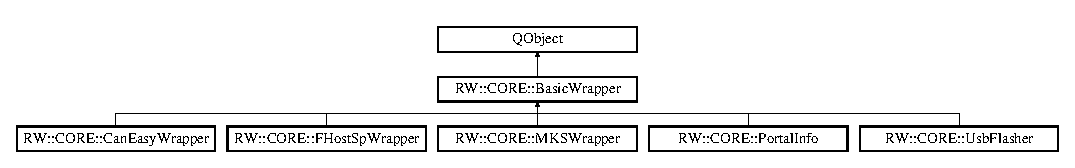
\includegraphics[height=1.806452cm]{class_r_w_1_1_c_o_r_e_1_1_basic_wrapper}
\end{center}
\end{figure}
\subsection*{Public Slots}
\begin{DoxyCompactItemize}
\item 
virtual void \hyperlink{class_r_w_1_1_c_o_r_e_1_1_basic_wrapper_a8541942f3b9c66acbc86c2d4310c622b}{On\+Process\+Message} (Util\+::\+Message\+Receiver Type, Util\+::\+Functions Func, Q\+Byte\+Array Report)=0
\end{DoxyCompactItemize}
\subsection*{Signals}
\begin{DoxyCompactItemize}
\item 
void \hyperlink{class_r_w_1_1_c_o_r_e_1_1_basic_wrapper_a9c59f7978bd65b16bff623f414fab06f}{New\+Message} (Util\+::\+Functions Func, Util\+::\+Error\+ID Message\+Type, Q\+Byte\+Array \hyperlink{namespace_r_w_1_1_c_o_r_e_a571834b44d0e3fab58aa6abfe5a02988}{Message})
\end{DoxyCompactItemize}
\subsection*{Public Member Functions}
\begin{DoxyCompactItemize}
\item 
\hyperlink{class_r_w_1_1_c_o_r_e_1_1_basic_wrapper_a637f4211c459a11dfc5e2564e3e706f8}{Basic\+Wrapper} (Q\+Object $\ast$Parent=nullptr)
\item 
virtual \hyperlink{class_r_w_1_1_c_o_r_e_1_1_basic_wrapper_aae30fea5f2a60ebd199be2c9fe2e691f}{$\sim$\+Basic\+Wrapper} ()
\end{DoxyCompactItemize}


\subsection{Detailed Description}


Definition at line 8 of file Basic\+Wrapper.\+h.



\subsection{Constructor \& Destructor Documentation}
\hypertarget{class_r_w_1_1_c_o_r_e_1_1_basic_wrapper_a637f4211c459a11dfc5e2564e3e706f8}{}\label{class_r_w_1_1_c_o_r_e_1_1_basic_wrapper_a637f4211c459a11dfc5e2564e3e706f8} 
\index{R\+W\+::\+C\+O\+R\+E\+::\+Basic\+Wrapper@{R\+W\+::\+C\+O\+R\+E\+::\+Basic\+Wrapper}!Basic\+Wrapper@{Basic\+Wrapper}}
\index{Basic\+Wrapper@{Basic\+Wrapper}!R\+W\+::\+C\+O\+R\+E\+::\+Basic\+Wrapper@{R\+W\+::\+C\+O\+R\+E\+::\+Basic\+Wrapper}}
\subsubsection{\texorpdfstring{Basic\+Wrapper()}{BasicWrapper()}}
{\footnotesize\ttfamily R\+W\+::\+C\+O\+R\+E\+::\+Basic\+Wrapper\+::\+Basic\+Wrapper (\begin{DoxyParamCaption}\item[{Q\+Object $\ast$}]{Parent = {\ttfamily nullptr} }\end{DoxyParamCaption})\hspace{0.3cm}{\ttfamily [inline]}}



Definition at line 13 of file Basic\+Wrapper.\+h.

\hypertarget{class_r_w_1_1_c_o_r_e_1_1_basic_wrapper_aae30fea5f2a60ebd199be2c9fe2e691f}{}\label{class_r_w_1_1_c_o_r_e_1_1_basic_wrapper_aae30fea5f2a60ebd199be2c9fe2e691f} 
\index{R\+W\+::\+C\+O\+R\+E\+::\+Basic\+Wrapper@{R\+W\+::\+C\+O\+R\+E\+::\+Basic\+Wrapper}!````~Basic\+Wrapper@{$\sim$\+Basic\+Wrapper}}
\index{````~Basic\+Wrapper@{$\sim$\+Basic\+Wrapper}!R\+W\+::\+C\+O\+R\+E\+::\+Basic\+Wrapper@{R\+W\+::\+C\+O\+R\+E\+::\+Basic\+Wrapper}}
\subsubsection{\texorpdfstring{$\sim$\+Basic\+Wrapper()}{~BasicWrapper()}}
{\footnotesize\ttfamily virtual R\+W\+::\+C\+O\+R\+E\+::\+Basic\+Wrapper\+::$\sim$\+Basic\+Wrapper (\begin{DoxyParamCaption}{ }\end{DoxyParamCaption})\hspace{0.3cm}{\ttfamily [inline]}, {\ttfamily [virtual]}}



Definition at line 15 of file Basic\+Wrapper.\+h.



\subsection{Member Function Documentation}
\hypertarget{class_r_w_1_1_c_o_r_e_1_1_basic_wrapper_a9c59f7978bd65b16bff623f414fab06f}{}\label{class_r_w_1_1_c_o_r_e_1_1_basic_wrapper_a9c59f7978bd65b16bff623f414fab06f} 
\index{R\+W\+::\+C\+O\+R\+E\+::\+Basic\+Wrapper@{R\+W\+::\+C\+O\+R\+E\+::\+Basic\+Wrapper}!New\+Message@{New\+Message}}
\index{New\+Message@{New\+Message}!R\+W\+::\+C\+O\+R\+E\+::\+Basic\+Wrapper@{R\+W\+::\+C\+O\+R\+E\+::\+Basic\+Wrapper}}
\subsubsection{\texorpdfstring{New\+Message}{NewMessage}}
{\footnotesize\ttfamily void R\+W\+::\+C\+O\+R\+E\+::\+Basic\+Wrapper\+::\+New\+Message (\begin{DoxyParamCaption}\item[{Util\+::\+Functions}]{Func,  }\item[{Util\+::\+Error\+ID}]{Message\+Type,  }\item[{Q\+Byte\+Array}]{Message }\end{DoxyParamCaption})\hspace{0.3cm}{\ttfamily [signal]}}



Definition at line 141 of file moc\+\_\+\+Basic\+Wrapper.\+cpp.

\hypertarget{class_r_w_1_1_c_o_r_e_1_1_basic_wrapper_a8541942f3b9c66acbc86c2d4310c622b}{}\label{class_r_w_1_1_c_o_r_e_1_1_basic_wrapper_a8541942f3b9c66acbc86c2d4310c622b} 
\index{R\+W\+::\+C\+O\+R\+E\+::\+Basic\+Wrapper@{R\+W\+::\+C\+O\+R\+E\+::\+Basic\+Wrapper}!On\+Process\+Message@{On\+Process\+Message}}
\index{On\+Process\+Message@{On\+Process\+Message}!R\+W\+::\+C\+O\+R\+E\+::\+Basic\+Wrapper@{R\+W\+::\+C\+O\+R\+E\+::\+Basic\+Wrapper}}
\subsubsection{\texorpdfstring{On\+Process\+Message}{OnProcessMessage}}
{\footnotesize\ttfamily virtual void R\+W\+::\+C\+O\+R\+E\+::\+Basic\+Wrapper\+::\+On\+Process\+Message (\begin{DoxyParamCaption}\item[{Util\+::\+Message\+Receiver}]{Type,  }\item[{Util\+::\+Functions}]{Func,  }\item[{Q\+Byte\+Array}]{Report }\end{DoxyParamCaption})\hspace{0.3cm}{\ttfamily [pure virtual]}, {\ttfamily [slot]}}



The documentation for this class was generated from the following files\+:\begin{DoxyCompactItemize}
\item 
C\+:/\+Projekte/\+Remote\+Repros/\+Remote\+Hidden\+Helper/\+Remote\+Hidden\+Helper/\hyperlink{_basic_wrapper_8h}{Basic\+Wrapper.\+h}\item 
C\+:/\+Projekte/\+Remote\+Repros/\+Remote\+Hidden\+Helper/\+Remote\+Hidden\+Helper/\+Generated\+Files/\+Debug/\hyperlink{_debug_2moc___basic_wrapper_8cpp}{moc\+\_\+\+Basic\+Wrapper.\+cpp}\end{DoxyCompactItemize}

\hypertarget{class_r_w_1_1_c_o_r_e_1_1_can_easy_wrapper}{}\section{RW\+:\+:C\+O\+RE\+:\+:Can\+Easy\+Wrapper Class Reference}
\label{class_r_w_1_1_c_o_r_e_1_1_can_easy_wrapper}\index{R\+W\+::\+C\+O\+R\+E\+::\+Can\+Easy\+Wrapper@{R\+W\+::\+C\+O\+R\+E\+::\+Can\+Easy\+Wrapper}}


{\ttfamily \#include $<$Can\+Easy\+Wrapper.\+h$>$}

Inheritance diagram for RW\+:\+:C\+O\+RE\+:\+:Can\+Easy\+Wrapper\+:\begin{figure}[H]
\begin{center}
\leavevmode
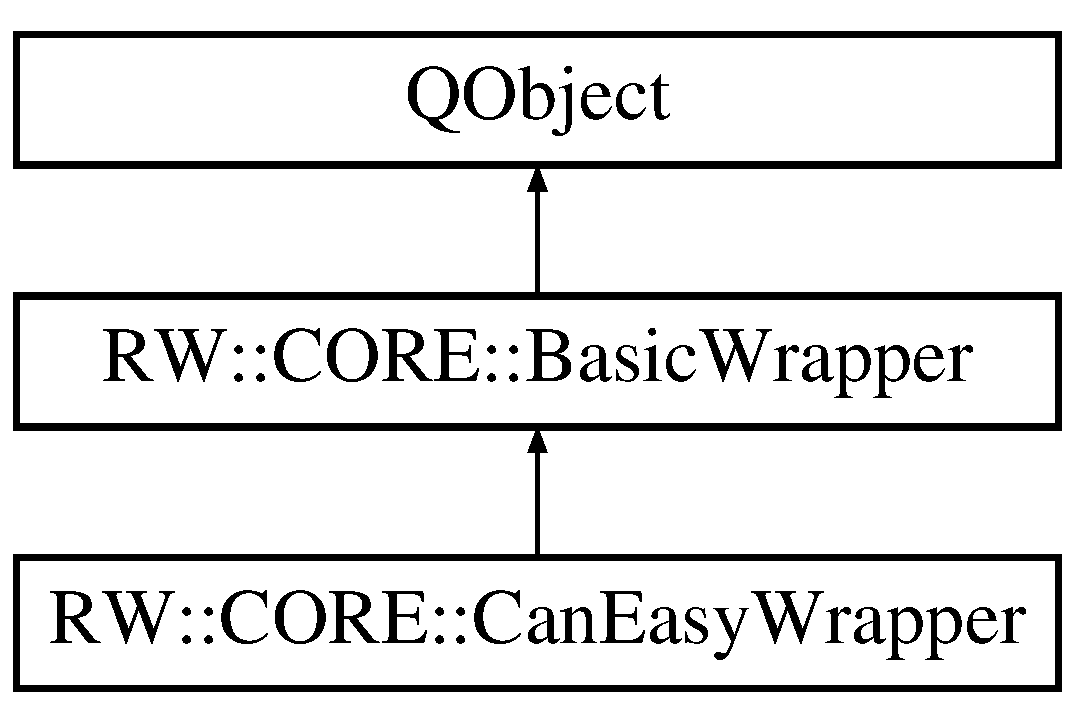
\includegraphics[height=3.000000cm]{class_r_w_1_1_c_o_r_e_1_1_can_easy_wrapper}
\end{center}
\end{figure}
\subsection*{Public Slots}
\begin{DoxyCompactItemize}
\item 
virtual void \hyperlink{class_r_w_1_1_c_o_r_e_1_1_can_easy_wrapper_a1de1ab208ac14badbf4b1483e7821801}{On\+Process\+Message} (Util\+::\+Message\+Receiver Type, Util\+::\+Functions Func, Q\+Byte\+Array Report)
\end{DoxyCompactItemize}
\subsection*{Public Member Functions}
\begin{DoxyCompactItemize}
\item 
\hyperlink{class_r_w_1_1_c_o_r_e_1_1_can_easy_wrapper_a2f8ebb5aeeca7a378a50b354cdb993fd}{Can\+Easy\+Wrapper} (Q\+Object $\ast$Parent=nullptr)
\item 
\hyperlink{class_r_w_1_1_c_o_r_e_1_1_can_easy_wrapper_af4170177b064c01efb78253f7ee78d86}{$\sim$\+Can\+Easy\+Wrapper} ()
\end{DoxyCompactItemize}
\subsection*{Private Member Functions}
\begin{DoxyCompactItemize}
\item 
void \hyperlink{class_r_w_1_1_c_o_r_e_1_1_can_easy_wrapper_a3dd585f435f8249429a1cd6c60f52037}{Start\+Can\+Easy} (const Q\+File \&Can\+Easy\+Installion\+Dir)
\item 
void \hyperlink{class_r_w_1_1_c_o_r_e_1_1_can_easy_wrapper_ad0bab30da2a3b67c624b82c0696d0d22}{Start\+Simulation} ()
\item 
void \hyperlink{class_r_w_1_1_c_o_r_e_1_1_can_easy_wrapper_a05dfab9becd44083a684df4e5f263b3d}{Stop\+Simulation} ()
\item 
void \hyperlink{class_r_w_1_1_c_o_r_e_1_1_can_easy_wrapper_aad31305e358aaaa21bfb93aeab5a3b33}{Load\+Workspace} (const Q\+File \&Workspace)
\item 
void \hyperlink{class_r_w_1_1_c_o_r_e_1_1_can_easy_wrapper_a2cdc4ca7e44bb4305455460743cf2496}{Stop\+Can\+Easy} ()
\item 
void \hyperlink{class_r_w_1_1_c_o_r_e_1_1_can_easy_wrapper_ab70adb2dc78f160412ec155c4ead3f15}{Close\+Explicit} ()
\end{DoxyCompactItemize}
\subsection*{Private Attributes}
\begin{DoxyCompactItemize}
\item 
C\+Com\+Ptr$<$ I\+Can\+Easy\+Process $>$ \hyperlink{class_r_w_1_1_c_o_r_e_1_1_can_easy_wrapper_ac2ed85324d592c81e797426cef3d600e}{m\+\_\+\+Process}
\item 
C\+Com\+Ptr$<$ I\+Can\+Easy\+Application $>$ \hyperlink{class_r_w_1_1_c_o_r_e_1_1_can_easy_wrapper_a263279df123f2f05d2752ccf6c62da18}{m\+\_\+\+App}
\item 
bool \hyperlink{class_r_w_1_1_c_o_r_e_1_1_can_easy_wrapper_a6bc2ad0752071fe7495bc971946a5a58}{m\+\_\+\+Is\+Running}
\end{DoxyCompactItemize}
\subsection*{Additional Inherited Members}


\subsection{Detailed Description}


Definition at line 13 of file Can\+Easy\+Wrapper.\+h.



\subsection{Constructor \& Destructor Documentation}
\hypertarget{class_r_w_1_1_c_o_r_e_1_1_can_easy_wrapper_a2f8ebb5aeeca7a378a50b354cdb993fd}{}\label{class_r_w_1_1_c_o_r_e_1_1_can_easy_wrapper_a2f8ebb5aeeca7a378a50b354cdb993fd} 
\index{R\+W\+::\+C\+O\+R\+E\+::\+Can\+Easy\+Wrapper@{R\+W\+::\+C\+O\+R\+E\+::\+Can\+Easy\+Wrapper}!Can\+Easy\+Wrapper@{Can\+Easy\+Wrapper}}
\index{Can\+Easy\+Wrapper@{Can\+Easy\+Wrapper}!R\+W\+::\+C\+O\+R\+E\+::\+Can\+Easy\+Wrapper@{R\+W\+::\+C\+O\+R\+E\+::\+Can\+Easy\+Wrapper}}
\subsubsection{\texorpdfstring{Can\+Easy\+Wrapper()}{CanEasyWrapper()}}
{\footnotesize\ttfamily R\+W\+::\+C\+O\+R\+E\+::\+Can\+Easy\+Wrapper\+::\+Can\+Easy\+Wrapper (\begin{DoxyParamCaption}\item[{Q\+Object $\ast$}]{Parent = {\ttfamily nullptr} }\end{DoxyParamCaption})}



Definition at line 8 of file Can\+Easy\+Wrapper.\+cpp.

\hypertarget{class_r_w_1_1_c_o_r_e_1_1_can_easy_wrapper_af4170177b064c01efb78253f7ee78d86}{}\label{class_r_w_1_1_c_o_r_e_1_1_can_easy_wrapper_af4170177b064c01efb78253f7ee78d86} 
\index{R\+W\+::\+C\+O\+R\+E\+::\+Can\+Easy\+Wrapper@{R\+W\+::\+C\+O\+R\+E\+::\+Can\+Easy\+Wrapper}!````~Can\+Easy\+Wrapper@{$\sim$\+Can\+Easy\+Wrapper}}
\index{````~Can\+Easy\+Wrapper@{$\sim$\+Can\+Easy\+Wrapper}!R\+W\+::\+C\+O\+R\+E\+::\+Can\+Easy\+Wrapper@{R\+W\+::\+C\+O\+R\+E\+::\+Can\+Easy\+Wrapper}}
\subsubsection{\texorpdfstring{$\sim$\+Can\+Easy\+Wrapper()}{~CanEasyWrapper()}}
{\footnotesize\ttfamily R\+W\+::\+C\+O\+R\+E\+::\+Can\+Easy\+Wrapper\+::$\sim$\+Can\+Easy\+Wrapper (\begin{DoxyParamCaption}{ }\end{DoxyParamCaption})}



Definition at line 14 of file Can\+Easy\+Wrapper.\+cpp.



\subsection{Member Function Documentation}
\hypertarget{class_r_w_1_1_c_o_r_e_1_1_can_easy_wrapper_ab70adb2dc78f160412ec155c4ead3f15}{}\label{class_r_w_1_1_c_o_r_e_1_1_can_easy_wrapper_ab70adb2dc78f160412ec155c4ead3f15} 
\index{R\+W\+::\+C\+O\+R\+E\+::\+Can\+Easy\+Wrapper@{R\+W\+::\+C\+O\+R\+E\+::\+Can\+Easy\+Wrapper}!Close\+Explicit@{Close\+Explicit}}
\index{Close\+Explicit@{Close\+Explicit}!R\+W\+::\+C\+O\+R\+E\+::\+Can\+Easy\+Wrapper@{R\+W\+::\+C\+O\+R\+E\+::\+Can\+Easy\+Wrapper}}
\subsubsection{\texorpdfstring{Close\+Explicit()}{CloseExplicit()}}
{\footnotesize\ttfamily void R\+W\+::\+C\+O\+R\+E\+::\+Can\+Easy\+Wrapper\+::\+Close\+Explicit (\begin{DoxyParamCaption}{ }\end{DoxyParamCaption})\hspace{0.3cm}{\ttfamily [private]}}



Definition at line 161 of file Can\+Easy\+Wrapper.\+cpp.

\hypertarget{class_r_w_1_1_c_o_r_e_1_1_can_easy_wrapper_aad31305e358aaaa21bfb93aeab5a3b33}{}\label{class_r_w_1_1_c_o_r_e_1_1_can_easy_wrapper_aad31305e358aaaa21bfb93aeab5a3b33} 
\index{R\+W\+::\+C\+O\+R\+E\+::\+Can\+Easy\+Wrapper@{R\+W\+::\+C\+O\+R\+E\+::\+Can\+Easy\+Wrapper}!Load\+Workspace@{Load\+Workspace}}
\index{Load\+Workspace@{Load\+Workspace}!R\+W\+::\+C\+O\+R\+E\+::\+Can\+Easy\+Wrapper@{R\+W\+::\+C\+O\+R\+E\+::\+Can\+Easy\+Wrapper}}
\subsubsection{\texorpdfstring{Load\+Workspace()}{LoadWorkspace()}}
{\footnotesize\ttfamily void R\+W\+::\+C\+O\+R\+E\+::\+Can\+Easy\+Wrapper\+::\+Load\+Workspace (\begin{DoxyParamCaption}\item[{const Q\+File \&}]{Workspace }\end{DoxyParamCaption})\hspace{0.3cm}{\ttfamily [private]}}



Definition at line 90 of file Can\+Easy\+Wrapper.\+cpp.

\hypertarget{class_r_w_1_1_c_o_r_e_1_1_can_easy_wrapper_a1de1ab208ac14badbf4b1483e7821801}{}\label{class_r_w_1_1_c_o_r_e_1_1_can_easy_wrapper_a1de1ab208ac14badbf4b1483e7821801} 
\index{R\+W\+::\+C\+O\+R\+E\+::\+Can\+Easy\+Wrapper@{R\+W\+::\+C\+O\+R\+E\+::\+Can\+Easy\+Wrapper}!On\+Process\+Message@{On\+Process\+Message}}
\index{On\+Process\+Message@{On\+Process\+Message}!R\+W\+::\+C\+O\+R\+E\+::\+Can\+Easy\+Wrapper@{R\+W\+::\+C\+O\+R\+E\+::\+Can\+Easy\+Wrapper}}
\subsubsection{\texorpdfstring{On\+Process\+Message}{OnProcessMessage}}
{\footnotesize\ttfamily void R\+W\+::\+C\+O\+R\+E\+::\+Can\+Easy\+Wrapper\+::\+On\+Process\+Message (\begin{DoxyParamCaption}\item[{Util\+::\+Message\+Receiver}]{Type,  }\item[{Util\+::\+Functions}]{Func,  }\item[{Q\+Byte\+Array}]{Report }\end{DoxyParamCaption})\hspace{0.3cm}{\ttfamily [virtual]}, {\ttfamily [slot]}}



Definition at line 18 of file Can\+Easy\+Wrapper.\+cpp.

\hypertarget{class_r_w_1_1_c_o_r_e_1_1_can_easy_wrapper_a3dd585f435f8249429a1cd6c60f52037}{}\label{class_r_w_1_1_c_o_r_e_1_1_can_easy_wrapper_a3dd585f435f8249429a1cd6c60f52037} 
\index{R\+W\+::\+C\+O\+R\+E\+::\+Can\+Easy\+Wrapper@{R\+W\+::\+C\+O\+R\+E\+::\+Can\+Easy\+Wrapper}!Start\+Can\+Easy@{Start\+Can\+Easy}}
\index{Start\+Can\+Easy@{Start\+Can\+Easy}!R\+W\+::\+C\+O\+R\+E\+::\+Can\+Easy\+Wrapper@{R\+W\+::\+C\+O\+R\+E\+::\+Can\+Easy\+Wrapper}}
\subsubsection{\texorpdfstring{Start\+Can\+Easy()}{StartCanEasy()}}
{\footnotesize\ttfamily void R\+W\+::\+C\+O\+R\+E\+::\+Can\+Easy\+Wrapper\+::\+Start\+Can\+Easy (\begin{DoxyParamCaption}\item[{const Q\+File \&}]{Can\+Easy\+Installion\+Dir }\end{DoxyParamCaption})\hspace{0.3cm}{\ttfamily [private]}}



Definition at line 45 of file Can\+Easy\+Wrapper.\+cpp.

\hypertarget{class_r_w_1_1_c_o_r_e_1_1_can_easy_wrapper_ad0bab30da2a3b67c624b82c0696d0d22}{}\label{class_r_w_1_1_c_o_r_e_1_1_can_easy_wrapper_ad0bab30da2a3b67c624b82c0696d0d22} 
\index{R\+W\+::\+C\+O\+R\+E\+::\+Can\+Easy\+Wrapper@{R\+W\+::\+C\+O\+R\+E\+::\+Can\+Easy\+Wrapper}!Start\+Simulation@{Start\+Simulation}}
\index{Start\+Simulation@{Start\+Simulation}!R\+W\+::\+C\+O\+R\+E\+::\+Can\+Easy\+Wrapper@{R\+W\+::\+C\+O\+R\+E\+::\+Can\+Easy\+Wrapper}}
\subsubsection{\texorpdfstring{Start\+Simulation()}{StartSimulation()}}
{\footnotesize\ttfamily void R\+W\+::\+C\+O\+R\+E\+::\+Can\+Easy\+Wrapper\+::\+Start\+Simulation (\begin{DoxyParamCaption}{ }\end{DoxyParamCaption})\hspace{0.3cm}{\ttfamily [private]}}



Definition at line 124 of file Can\+Easy\+Wrapper.\+cpp.

\hypertarget{class_r_w_1_1_c_o_r_e_1_1_can_easy_wrapper_a2cdc4ca7e44bb4305455460743cf2496}{}\label{class_r_w_1_1_c_o_r_e_1_1_can_easy_wrapper_a2cdc4ca7e44bb4305455460743cf2496} 
\index{R\+W\+::\+C\+O\+R\+E\+::\+Can\+Easy\+Wrapper@{R\+W\+::\+C\+O\+R\+E\+::\+Can\+Easy\+Wrapper}!Stop\+Can\+Easy@{Stop\+Can\+Easy}}
\index{Stop\+Can\+Easy@{Stop\+Can\+Easy}!R\+W\+::\+C\+O\+R\+E\+::\+Can\+Easy\+Wrapper@{R\+W\+::\+C\+O\+R\+E\+::\+Can\+Easy\+Wrapper}}
\subsubsection{\texorpdfstring{Stop\+Can\+Easy()}{StopCanEasy()}}
{\footnotesize\ttfamily void R\+W\+::\+C\+O\+R\+E\+::\+Can\+Easy\+Wrapper\+::\+Stop\+Can\+Easy (\begin{DoxyParamCaption}{ }\end{DoxyParamCaption})\hspace{0.3cm}{\ttfamily [private]}}



Definition at line 109 of file Can\+Easy\+Wrapper.\+cpp.

\hypertarget{class_r_w_1_1_c_o_r_e_1_1_can_easy_wrapper_a05dfab9becd44083a684df4e5f263b3d}{}\label{class_r_w_1_1_c_o_r_e_1_1_can_easy_wrapper_a05dfab9becd44083a684df4e5f263b3d} 
\index{R\+W\+::\+C\+O\+R\+E\+::\+Can\+Easy\+Wrapper@{R\+W\+::\+C\+O\+R\+E\+::\+Can\+Easy\+Wrapper}!Stop\+Simulation@{Stop\+Simulation}}
\index{Stop\+Simulation@{Stop\+Simulation}!R\+W\+::\+C\+O\+R\+E\+::\+Can\+Easy\+Wrapper@{R\+W\+::\+C\+O\+R\+E\+::\+Can\+Easy\+Wrapper}}
\subsubsection{\texorpdfstring{Stop\+Simulation()}{StopSimulation()}}
{\footnotesize\ttfamily void R\+W\+::\+C\+O\+R\+E\+::\+Can\+Easy\+Wrapper\+::\+Stop\+Simulation (\begin{DoxyParamCaption}{ }\end{DoxyParamCaption})\hspace{0.3cm}{\ttfamily [private]}}



Definition at line 143 of file Can\+Easy\+Wrapper.\+cpp.



\subsection{Member Data Documentation}
\hypertarget{class_r_w_1_1_c_o_r_e_1_1_can_easy_wrapper_a263279df123f2f05d2752ccf6c62da18}{}\label{class_r_w_1_1_c_o_r_e_1_1_can_easy_wrapper_a263279df123f2f05d2752ccf6c62da18} 
\index{R\+W\+::\+C\+O\+R\+E\+::\+Can\+Easy\+Wrapper@{R\+W\+::\+C\+O\+R\+E\+::\+Can\+Easy\+Wrapper}!m\+\_\+\+App@{m\+\_\+\+App}}
\index{m\+\_\+\+App@{m\+\_\+\+App}!R\+W\+::\+C\+O\+R\+E\+::\+Can\+Easy\+Wrapper@{R\+W\+::\+C\+O\+R\+E\+::\+Can\+Easy\+Wrapper}}
\subsubsection{\texorpdfstring{m\+\_\+\+App}{m\_App}}
{\footnotesize\ttfamily C\+Com\+Ptr$<$I\+Can\+Easy\+Application$>$ R\+W\+::\+C\+O\+R\+E\+::\+Can\+Easy\+Wrapper\+::m\+\_\+\+App\hspace{0.3cm}{\ttfamily [private]}}



Definition at line 19 of file Can\+Easy\+Wrapper.\+h.

\hypertarget{class_r_w_1_1_c_o_r_e_1_1_can_easy_wrapper_a6bc2ad0752071fe7495bc971946a5a58}{}\label{class_r_w_1_1_c_o_r_e_1_1_can_easy_wrapper_a6bc2ad0752071fe7495bc971946a5a58} 
\index{R\+W\+::\+C\+O\+R\+E\+::\+Can\+Easy\+Wrapper@{R\+W\+::\+C\+O\+R\+E\+::\+Can\+Easy\+Wrapper}!m\+\_\+\+Is\+Running@{m\+\_\+\+Is\+Running}}
\index{m\+\_\+\+Is\+Running@{m\+\_\+\+Is\+Running}!R\+W\+::\+C\+O\+R\+E\+::\+Can\+Easy\+Wrapper@{R\+W\+::\+C\+O\+R\+E\+::\+Can\+Easy\+Wrapper}}
\subsubsection{\texorpdfstring{m\+\_\+\+Is\+Running}{m\_IsRunning}}
{\footnotesize\ttfamily bool R\+W\+::\+C\+O\+R\+E\+::\+Can\+Easy\+Wrapper\+::m\+\_\+\+Is\+Running\hspace{0.3cm}{\ttfamily [private]}}



Definition at line 20 of file Can\+Easy\+Wrapper.\+h.

\hypertarget{class_r_w_1_1_c_o_r_e_1_1_can_easy_wrapper_ac2ed85324d592c81e797426cef3d600e}{}\label{class_r_w_1_1_c_o_r_e_1_1_can_easy_wrapper_ac2ed85324d592c81e797426cef3d600e} 
\index{R\+W\+::\+C\+O\+R\+E\+::\+Can\+Easy\+Wrapper@{R\+W\+::\+C\+O\+R\+E\+::\+Can\+Easy\+Wrapper}!m\+\_\+\+Process@{m\+\_\+\+Process}}
\index{m\+\_\+\+Process@{m\+\_\+\+Process}!R\+W\+::\+C\+O\+R\+E\+::\+Can\+Easy\+Wrapper@{R\+W\+::\+C\+O\+R\+E\+::\+Can\+Easy\+Wrapper}}
\subsubsection{\texorpdfstring{m\+\_\+\+Process}{m\_Process}}
{\footnotesize\ttfamily C\+Com\+Ptr$<$I\+Can\+Easy\+Process$>$ R\+W\+::\+C\+O\+R\+E\+::\+Can\+Easy\+Wrapper\+::m\+\_\+\+Process\hspace{0.3cm}{\ttfamily [private]}}



Definition at line 18 of file Can\+Easy\+Wrapper.\+h.



The documentation for this class was generated from the following files\+:\begin{DoxyCompactItemize}
\item 
C\+:/\+Projekte/\+Remote\+Repros/\+Remote\+Hidden\+Helper/\+Remote\+Hidden\+Helper/\hyperlink{_can_easy_wrapper_8h}{Can\+Easy\+Wrapper.\+h}\item 
C\+:/\+Projekte/\+Remote\+Repros/\+Remote\+Hidden\+Helper/\+Remote\+Hidden\+Helper/\hyperlink{_can_easy_wrapper_8cpp}{Can\+Easy\+Wrapper.\+cpp}\end{DoxyCompactItemize}

\hypertarget{class_r_w_1_1_c_o_r_e_1_1_communication_manager}{}\section{RW\+:\+:C\+O\+RE\+:\+:Communication\+Manager Class Reference}
\label{class_r_w_1_1_c_o_r_e_1_1_communication_manager}\index{R\+W\+::\+C\+O\+R\+E\+::\+Communication\+Manager@{R\+W\+::\+C\+O\+R\+E\+::\+Communication\+Manager}}


{\ttfamily \#include $<$Communication\+Manager.\+h$>$}

Inheritance diagram for RW\+:\+:C\+O\+RE\+:\+:Communication\+Manager\+:\begin{figure}[H]
\begin{center}
\leavevmode
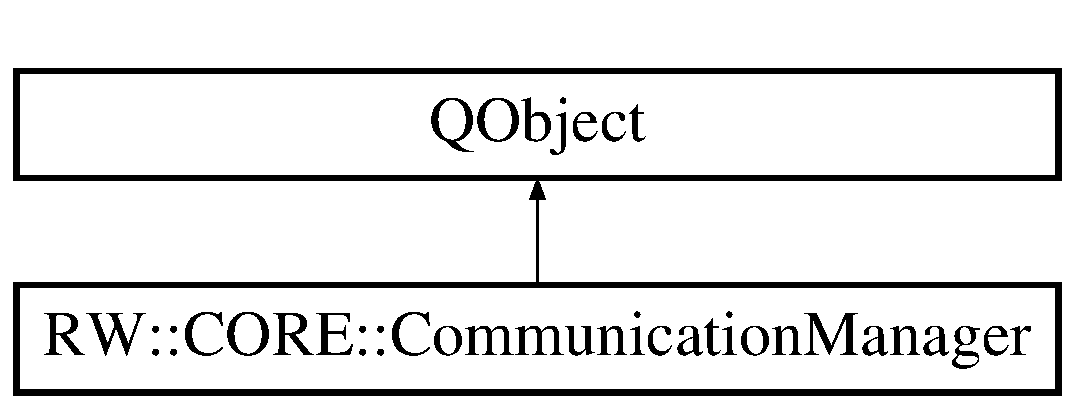
\includegraphics[height=2.000000cm]{class_r_w_1_1_c_o_r_e_1_1_communication_manager}
\end{center}
\end{figure}
\subsection*{Public Slots}
\begin{DoxyCompactItemize}
\item 
void \hyperlink{class_r_w_1_1_c_o_r_e_1_1_communication_manager_a7c890fda317487cb2892d728e0b7e131}{On\+Process\+Message\+Answer} (Util\+::\+Functions Func, Util\+::\+Error\+ID Id, Q\+Byte\+Array \hyperlink{namespace_r_w_1_1_c_o_r_e_a571834b44d0e3fab58aa6abfe5a02988}{Message})
\end{DoxyCompactItemize}
\subsection*{Signals}
\begin{DoxyCompactItemize}
\item 
void \hyperlink{class_r_w_1_1_c_o_r_e_1_1_communication_manager_aae001b1bddaf9c74f20795f6954432b9}{New\+Message} (Util\+::\+Message\+Receiver Type, Util\+::\+Functions Func, Q\+Byte\+Array Report)
\end{DoxyCompactItemize}
\subsection*{Public Member Functions}
\begin{DoxyCompactItemize}
\item 
\hyperlink{class_r_w_1_1_c_o_r_e_1_1_communication_manager_a8afb1aacf5b5d582256afdda0d191d91}{Communication\+Manager} (\hyperlink{class_r_w_1_1_c_o_r_e_1_1_error_handler}{Error\+Handler} $\ast$\hyperlink{class_r_w_1_1_c_o_r_e_1_1_error_handler}{Error\+Handler}, Q\+Object $\ast$Parent=nullptr)
\item 
\hyperlink{class_r_w_1_1_c_o_r_e_1_1_communication_manager_a4fc7eed7b4e58d01100820e21eb19f57}{$\sim$\+Communication\+Manager} ()
\end{DoxyCompactItemize}
\subsection*{Private Slots}
\begin{DoxyCompactItemize}
\item 
void \hyperlink{class_r_w_1_1_c_o_r_e_1_1_communication_manager_a3f3cff8fe51bc3eeb7d93d22e5061c06}{On\+Process\+Message} (Util\+::\+Functions Message\+Type, Q\+Byte\+Array \hyperlink{namespace_r_w_1_1_c_o_r_e_a571834b44d0e3fab58aa6abfe5a02988}{Message})
\end{DoxyCompactItemize}
\subsection*{Private Member Functions}
\begin{DoxyCompactItemize}
\item 
Q\+Byte\+Array \hyperlink{class_r_w_1_1_c_o_r_e_1_1_communication_manager_a496af2c201ed48e14033b640cf78ed3f}{Create\+Message} (Util\+::\+Functions Func, Q\+Byte\+Array \hyperlink{namespace_r_w_1_1_c_o_r_e_a571834b44d0e3fab58aa6abfe5a02988}{Message}, Util\+::\+Error\+ID Id)
\end{DoxyCompactItemize}
\subsection*{Private Attributes}
\begin{DoxyCompactItemize}
\item 
\hyperlink{class_r_w_1_1_c_o_r_e_1_1_communication_server}{Communication\+Server} $\ast$ \hyperlink{class_r_w_1_1_c_o_r_e_1_1_communication_manager_ae16c353628da4af164f91c9dd38cefac}{m\+\_\+\+Server}
\item 
\hyperlink{class_r_w_1_1_c_o_r_e_1_1_error_handler}{Error\+Handler} $\ast$ \hyperlink{class_r_w_1_1_c_o_r_e_1_1_communication_manager_ab4035d32b76f3856ba059bed7261ae85}{m\+\_\+\+Error\+Handler}
\end{DoxyCompactItemize}


\subsection{Detailed Description}


Definition at line 10 of file Communication\+Manager.\+h.



\subsection{Constructor \& Destructor Documentation}
\hypertarget{class_r_w_1_1_c_o_r_e_1_1_communication_manager_a8afb1aacf5b5d582256afdda0d191d91}{}\label{class_r_w_1_1_c_o_r_e_1_1_communication_manager_a8afb1aacf5b5d582256afdda0d191d91} 
\index{R\+W\+::\+C\+O\+R\+E\+::\+Communication\+Manager@{R\+W\+::\+C\+O\+R\+E\+::\+Communication\+Manager}!Communication\+Manager@{Communication\+Manager}}
\index{Communication\+Manager@{Communication\+Manager}!R\+W\+::\+C\+O\+R\+E\+::\+Communication\+Manager@{R\+W\+::\+C\+O\+R\+E\+::\+Communication\+Manager}}
\subsubsection{\texorpdfstring{Communication\+Manager()}{CommunicationManager()}}
{\footnotesize\ttfamily R\+W\+::\+C\+O\+R\+E\+::\+Communication\+Manager\+::\+Communication\+Manager (\begin{DoxyParamCaption}\item[{\hyperlink{class_r_w_1_1_c_o_r_e_1_1_error_handler}{Error\+Handler} $\ast$}]{Error\+Handler,  }\item[{Q\+Object $\ast$}]{Parent = {\ttfamily nullptr} }\end{DoxyParamCaption})}



Definition at line 9 of file Communication\+Manager.\+cpp.

\hypertarget{class_r_w_1_1_c_o_r_e_1_1_communication_manager_a4fc7eed7b4e58d01100820e21eb19f57}{}\label{class_r_w_1_1_c_o_r_e_1_1_communication_manager_a4fc7eed7b4e58d01100820e21eb19f57} 
\index{R\+W\+::\+C\+O\+R\+E\+::\+Communication\+Manager@{R\+W\+::\+C\+O\+R\+E\+::\+Communication\+Manager}!````~Communication\+Manager@{$\sim$\+Communication\+Manager}}
\index{````~Communication\+Manager@{$\sim$\+Communication\+Manager}!R\+W\+::\+C\+O\+R\+E\+::\+Communication\+Manager@{R\+W\+::\+C\+O\+R\+E\+::\+Communication\+Manager}}
\subsubsection{\texorpdfstring{$\sim$\+Communication\+Manager()}{~CommunicationManager()}}
{\footnotesize\ttfamily R\+W\+::\+C\+O\+R\+E\+::\+Communication\+Manager\+::$\sim$\+Communication\+Manager (\begin{DoxyParamCaption}{ }\end{DoxyParamCaption})}



Definition at line 18 of file Communication\+Manager.\+cpp.



\subsection{Member Function Documentation}
\hypertarget{class_r_w_1_1_c_o_r_e_1_1_communication_manager_a496af2c201ed48e14033b640cf78ed3f}{}\label{class_r_w_1_1_c_o_r_e_1_1_communication_manager_a496af2c201ed48e14033b640cf78ed3f} 
\index{R\+W\+::\+C\+O\+R\+E\+::\+Communication\+Manager@{R\+W\+::\+C\+O\+R\+E\+::\+Communication\+Manager}!Create\+Message@{Create\+Message}}
\index{Create\+Message@{Create\+Message}!R\+W\+::\+C\+O\+R\+E\+::\+Communication\+Manager@{R\+W\+::\+C\+O\+R\+E\+::\+Communication\+Manager}}
\subsubsection{\texorpdfstring{Create\+Message()}{CreateMessage()}}
{\footnotesize\ttfamily Q\+Byte\+Array R\+W\+::\+C\+O\+R\+E\+::\+Communication\+Manager\+::\+Create\+Message (\begin{DoxyParamCaption}\item[{Util\+::\+Functions}]{Func,  }\item[{Q\+Byte\+Array}]{Message,  }\item[{Util\+::\+Error\+ID}]{Id }\end{DoxyParamCaption})\hspace{0.3cm}{\ttfamily [private]}}



Definition at line 146 of file Communication\+Manager.\+cpp.

\hypertarget{class_r_w_1_1_c_o_r_e_1_1_communication_manager_aae001b1bddaf9c74f20795f6954432b9}{}\label{class_r_w_1_1_c_o_r_e_1_1_communication_manager_aae001b1bddaf9c74f20795f6954432b9} 
\index{R\+W\+::\+C\+O\+R\+E\+::\+Communication\+Manager@{R\+W\+::\+C\+O\+R\+E\+::\+Communication\+Manager}!New\+Message@{New\+Message}}
\index{New\+Message@{New\+Message}!R\+W\+::\+C\+O\+R\+E\+::\+Communication\+Manager@{R\+W\+::\+C\+O\+R\+E\+::\+Communication\+Manager}}
\subsubsection{\texorpdfstring{New\+Message}{NewMessage}}
{\footnotesize\ttfamily void R\+W\+::\+C\+O\+R\+E\+::\+Communication\+Manager\+::\+New\+Message (\begin{DoxyParamCaption}\item[{Util\+::\+Message\+Receiver}]{Type,  }\item[{Util\+::\+Functions}]{Func,  }\item[{Q\+Byte\+Array}]{Report }\end{DoxyParamCaption})\hspace{0.3cm}{\ttfamily [signal]}}



Definition at line 148 of file moc\+\_\+\+Communication\+Manager.\+cpp.

\hypertarget{class_r_w_1_1_c_o_r_e_1_1_communication_manager_a3f3cff8fe51bc3eeb7d93d22e5061c06}{}\label{class_r_w_1_1_c_o_r_e_1_1_communication_manager_a3f3cff8fe51bc3eeb7d93d22e5061c06} 
\index{R\+W\+::\+C\+O\+R\+E\+::\+Communication\+Manager@{R\+W\+::\+C\+O\+R\+E\+::\+Communication\+Manager}!On\+Process\+Message@{On\+Process\+Message}}
\index{On\+Process\+Message@{On\+Process\+Message}!R\+W\+::\+C\+O\+R\+E\+::\+Communication\+Manager@{R\+W\+::\+C\+O\+R\+E\+::\+Communication\+Manager}}
\subsubsection{\texorpdfstring{On\+Process\+Message}{OnProcessMessage}}
{\footnotesize\ttfamily void R\+W\+::\+C\+O\+R\+E\+::\+Communication\+Manager\+::\+On\+Process\+Message (\begin{DoxyParamCaption}\item[{Util\+::\+Functions}]{Message\+Type,  }\item[{Q\+Byte\+Array}]{Message }\end{DoxyParamCaption})\hspace{0.3cm}{\ttfamily [private]}, {\ttfamily [slot]}}



Definition at line 23 of file Communication\+Manager.\+cpp.

\hypertarget{class_r_w_1_1_c_o_r_e_1_1_communication_manager_a7c890fda317487cb2892d728e0b7e131}{}\label{class_r_w_1_1_c_o_r_e_1_1_communication_manager_a7c890fda317487cb2892d728e0b7e131} 
\index{R\+W\+::\+C\+O\+R\+E\+::\+Communication\+Manager@{R\+W\+::\+C\+O\+R\+E\+::\+Communication\+Manager}!On\+Process\+Message\+Answer@{On\+Process\+Message\+Answer}}
\index{On\+Process\+Message\+Answer@{On\+Process\+Message\+Answer}!R\+W\+::\+C\+O\+R\+E\+::\+Communication\+Manager@{R\+W\+::\+C\+O\+R\+E\+::\+Communication\+Manager}}
\subsubsection{\texorpdfstring{On\+Process\+Message\+Answer}{OnProcessMessageAnswer}}
{\footnotesize\ttfamily void R\+W\+::\+C\+O\+R\+E\+::\+Communication\+Manager\+::\+On\+Process\+Message\+Answer (\begin{DoxyParamCaption}\item[{Util\+::\+Functions}]{Func,  }\item[{Util\+::\+Error\+ID}]{Id,  }\item[{Q\+Byte\+Array}]{Message }\end{DoxyParamCaption})\hspace{0.3cm}{\ttfamily [slot]}}



Definition at line 132 of file Communication\+Manager.\+cpp.



\subsection{Member Data Documentation}
\hypertarget{class_r_w_1_1_c_o_r_e_1_1_communication_manager_ab4035d32b76f3856ba059bed7261ae85}{}\label{class_r_w_1_1_c_o_r_e_1_1_communication_manager_ab4035d32b76f3856ba059bed7261ae85} 
\index{R\+W\+::\+C\+O\+R\+E\+::\+Communication\+Manager@{R\+W\+::\+C\+O\+R\+E\+::\+Communication\+Manager}!m\+\_\+\+Error\+Handler@{m\+\_\+\+Error\+Handler}}
\index{m\+\_\+\+Error\+Handler@{m\+\_\+\+Error\+Handler}!R\+W\+::\+C\+O\+R\+E\+::\+Communication\+Manager@{R\+W\+::\+C\+O\+R\+E\+::\+Communication\+Manager}}
\subsubsection{\texorpdfstring{m\+\_\+\+Error\+Handler}{m\_ErrorHandler}}
{\footnotesize\ttfamily \hyperlink{class_r_w_1_1_c_o_r_e_1_1_error_handler}{Error\+Handler}$\ast$ R\+W\+::\+C\+O\+R\+E\+::\+Communication\+Manager\+::m\+\_\+\+Error\+Handler\hspace{0.3cm}{\ttfamily [private]}}



Definition at line 16 of file Communication\+Manager.\+h.

\hypertarget{class_r_w_1_1_c_o_r_e_1_1_communication_manager_ae16c353628da4af164f91c9dd38cefac}{}\label{class_r_w_1_1_c_o_r_e_1_1_communication_manager_ae16c353628da4af164f91c9dd38cefac} 
\index{R\+W\+::\+C\+O\+R\+E\+::\+Communication\+Manager@{R\+W\+::\+C\+O\+R\+E\+::\+Communication\+Manager}!m\+\_\+\+Server@{m\+\_\+\+Server}}
\index{m\+\_\+\+Server@{m\+\_\+\+Server}!R\+W\+::\+C\+O\+R\+E\+::\+Communication\+Manager@{R\+W\+::\+C\+O\+R\+E\+::\+Communication\+Manager}}
\subsubsection{\texorpdfstring{m\+\_\+\+Server}{m\_Server}}
{\footnotesize\ttfamily \hyperlink{class_r_w_1_1_c_o_r_e_1_1_communication_server}{Communication\+Server}$\ast$ R\+W\+::\+C\+O\+R\+E\+::\+Communication\+Manager\+::m\+\_\+\+Server\hspace{0.3cm}{\ttfamily [private]}}



Definition at line 15 of file Communication\+Manager.\+h.



The documentation for this class was generated from the following files\+:\begin{DoxyCompactItemize}
\item 
C\+:/\+Projekte/\+Remote\+Repros/\+Remote\+Hidden\+Helper/\+Remote\+Hidden\+Helper/\hyperlink{_communication_manager_8h}{Communication\+Manager.\+h}\item 
C\+:/\+Projekte/\+Remote\+Repros/\+Remote\+Hidden\+Helper/\+Remote\+Hidden\+Helper/\hyperlink{_communication_manager_8cpp}{Communication\+Manager.\+cpp}\item 
C\+:/\+Projekte/\+Remote\+Repros/\+Remote\+Hidden\+Helper/\+Remote\+Hidden\+Helper/\+Generated\+Files/\+Debug/\hyperlink{_debug_2moc___communication_manager_8cpp}{moc\+\_\+\+Communication\+Manager.\+cpp}\end{DoxyCompactItemize}

\hypertarget{class_r_w_1_1_c_o_r_e_1_1_communication_server}{}\section{RW\+:\+:C\+O\+RE\+:\+:Communication\+Server Class Reference}
\label{class_r_w_1_1_c_o_r_e_1_1_communication_server}\index{R\+W\+::\+C\+O\+R\+E\+::\+Communication\+Server@{R\+W\+::\+C\+O\+R\+E\+::\+Communication\+Server}}


{\ttfamily \#include $<$Communication\+Server.\+h$>$}

Inheritance diagram for RW\+:\+:C\+O\+RE\+:\+:Communication\+Server\+:\begin{figure}[H]
\begin{center}
\leavevmode
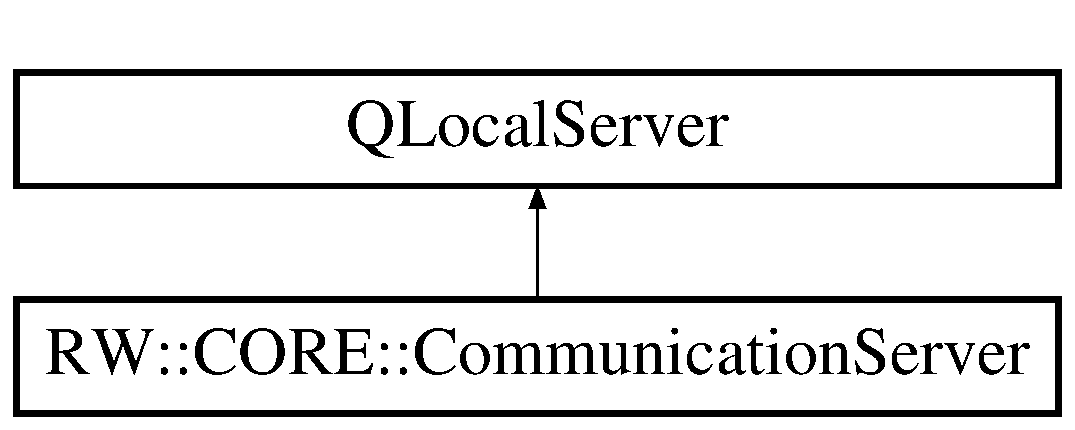
\includegraphics[height=2.000000cm]{class_r_w_1_1_c_o_r_e_1_1_communication_server}
\end{center}
\end{figure}
\subsection*{Public Slots}
\begin{DoxyCompactItemize}
\item 
void \hyperlink{class_r_w_1_1_c_o_r_e_1_1_communication_server_a623ab8380a69de4f849c284e808b30c0}{On\+Process\+Message} (Util\+::\+Message\+Receiver Type, Util\+::\+Functions Func, Q\+Byte\+Array \hyperlink{namespace_r_w_1_1_c_o_r_e_a571834b44d0e3fab58aa6abfe5a02988}{Message})
\end{DoxyCompactItemize}
\subsection*{Signals}
\begin{DoxyCompactItemize}
\item 
void \hyperlink{class_r_w_1_1_c_o_r_e_1_1_communication_server_a44354b19e6c0aad3f462904978b671a3}{New\+Message} (Util\+::\+Functions Message\+Type, Q\+Byte\+Array \hyperlink{namespace_r_w_1_1_c_o_r_e_a571834b44d0e3fab58aa6abfe5a02988}{Message})
\end{DoxyCompactItemize}
\subsection*{Public Member Functions}
\begin{DoxyCompactItemize}
\item 
\hyperlink{class_r_w_1_1_c_o_r_e_1_1_communication_server_a8b4be098b0e453dd10e717788dfd12b6}{Communication\+Server} (Q\+Object $\ast$Parent=nullptr)
\item 
\hyperlink{class_r_w_1_1_c_o_r_e_1_1_communication_server_a924f4957db6e0ae05d20520cdbc7e775}{$\sim$\+Communication\+Server} ()
\item 
bool \hyperlink{class_r_w_1_1_c_o_r_e_1_1_communication_server_a202a8635256a2ce503019a664917b095}{Init} ()
\item 
bool \hyperlink{class_r_w_1_1_c_o_r_e_1_1_communication_server_ac7b0fd62b6071c494f132e1a9e312604}{De\+Init} ()
\end{DoxyCompactItemize}
\subsection*{Private Member Functions}
\begin{DoxyCompactItemize}
\item 
void \hyperlink{class_r_w_1_1_c_o_r_e_1_1_communication_server_ad26258ff2481b68cec6d80e78e0a5c7d}{On\+New\+Connection} ()
\item 
void \hyperlink{class_r_w_1_1_c_o_r_e_1_1_communication_server_ae204445cecf0ff7a01409bd34a127f61}{On\+Client\+Disconnected} ()
\item 
void \hyperlink{class_r_w_1_1_c_o_r_e_1_1_communication_server_a1d852ba8f1b04e0e2e49b369c0f1d32d}{On\+Client\+Socket\+Error} (Q\+Local\+Socket\+::\+Local\+Socket\+Error socket\+Error)
\item 
void \hyperlink{class_r_w_1_1_c_o_r_e_1_1_communication_server_abdbb4f3eeced8215b50e75fdd93d62af}{On\+Data\+Available} ()
\item 
void \hyperlink{class_r_w_1_1_c_o_r_e_1_1_communication_server_a731de143323e7949781411506ed57891}{Send\+Message} (Q\+Byte\+Array Report)
\end{DoxyCompactItemize}
\subsection*{Private Attributes}
\begin{DoxyCompactItemize}
\item 
Q\+Local\+Socket $\ast$ \hyperlink{class_r_w_1_1_c_o_r_e_1_1_communication_server_a00d7ca97061231176a915058cf71d794}{m\+\_\+\+Client}
\end{DoxyCompactItemize}


\subsection{Detailed Description}


Definition at line 12 of file Communication\+Server.\+h.



\subsection{Constructor \& Destructor Documentation}
\hypertarget{class_r_w_1_1_c_o_r_e_1_1_communication_server_a8b4be098b0e453dd10e717788dfd12b6}{}\label{class_r_w_1_1_c_o_r_e_1_1_communication_server_a8b4be098b0e453dd10e717788dfd12b6} 
\index{R\+W\+::\+C\+O\+R\+E\+::\+Communication\+Server@{R\+W\+::\+C\+O\+R\+E\+::\+Communication\+Server}!Communication\+Server@{Communication\+Server}}
\index{Communication\+Server@{Communication\+Server}!R\+W\+::\+C\+O\+R\+E\+::\+Communication\+Server@{R\+W\+::\+C\+O\+R\+E\+::\+Communication\+Server}}
\subsubsection{\texorpdfstring{Communication\+Server()}{CommunicationServer()}}
{\footnotesize\ttfamily R\+W\+::\+C\+O\+R\+E\+::\+Communication\+Server\+::\+Communication\+Server (\begin{DoxyParamCaption}\item[{Q\+Object $\ast$}]{Parent = {\ttfamily nullptr} }\end{DoxyParamCaption})}



Definition at line 10 of file Communication\+Server.\+cpp.

\hypertarget{class_r_w_1_1_c_o_r_e_1_1_communication_server_a924f4957db6e0ae05d20520cdbc7e775}{}\label{class_r_w_1_1_c_o_r_e_1_1_communication_server_a924f4957db6e0ae05d20520cdbc7e775} 
\index{R\+W\+::\+C\+O\+R\+E\+::\+Communication\+Server@{R\+W\+::\+C\+O\+R\+E\+::\+Communication\+Server}!````~Communication\+Server@{$\sim$\+Communication\+Server}}
\index{````~Communication\+Server@{$\sim$\+Communication\+Server}!R\+W\+::\+C\+O\+R\+E\+::\+Communication\+Server@{R\+W\+::\+C\+O\+R\+E\+::\+Communication\+Server}}
\subsubsection{\texorpdfstring{$\sim$\+Communication\+Server()}{~CommunicationServer()}}
{\footnotesize\ttfamily R\+W\+::\+C\+O\+R\+E\+::\+Communication\+Server\+::$\sim$\+Communication\+Server (\begin{DoxyParamCaption}{ }\end{DoxyParamCaption})}



Definition at line 15 of file Communication\+Server.\+cpp.



\subsection{Member Function Documentation}
\hypertarget{class_r_w_1_1_c_o_r_e_1_1_communication_server_ac7b0fd62b6071c494f132e1a9e312604}{}\label{class_r_w_1_1_c_o_r_e_1_1_communication_server_ac7b0fd62b6071c494f132e1a9e312604} 
\index{R\+W\+::\+C\+O\+R\+E\+::\+Communication\+Server@{R\+W\+::\+C\+O\+R\+E\+::\+Communication\+Server}!De\+Init@{De\+Init}}
\index{De\+Init@{De\+Init}!R\+W\+::\+C\+O\+R\+E\+::\+Communication\+Server@{R\+W\+::\+C\+O\+R\+E\+::\+Communication\+Server}}
\subsubsection{\texorpdfstring{De\+Init()}{DeInit()}}
{\footnotesize\ttfamily bool R\+W\+::\+C\+O\+R\+E\+::\+Communication\+Server\+::\+De\+Init (\begin{DoxyParamCaption}{ }\end{DoxyParamCaption})}



Definition at line 41 of file Communication\+Server.\+cpp.

\hypertarget{class_r_w_1_1_c_o_r_e_1_1_communication_server_a202a8635256a2ce503019a664917b095}{}\label{class_r_w_1_1_c_o_r_e_1_1_communication_server_a202a8635256a2ce503019a664917b095} 
\index{R\+W\+::\+C\+O\+R\+E\+::\+Communication\+Server@{R\+W\+::\+C\+O\+R\+E\+::\+Communication\+Server}!Init@{Init}}
\index{Init@{Init}!R\+W\+::\+C\+O\+R\+E\+::\+Communication\+Server@{R\+W\+::\+C\+O\+R\+E\+::\+Communication\+Server}}
\subsubsection{\texorpdfstring{Init()}{Init()}}
{\footnotesize\ttfamily bool R\+W\+::\+C\+O\+R\+E\+::\+Communication\+Server\+::\+Init (\begin{DoxyParamCaption}{ }\end{DoxyParamCaption})}



Definition at line 19 of file Communication\+Server.\+cpp.

\hypertarget{class_r_w_1_1_c_o_r_e_1_1_communication_server_a44354b19e6c0aad3f462904978b671a3}{}\label{class_r_w_1_1_c_o_r_e_1_1_communication_server_a44354b19e6c0aad3f462904978b671a3} 
\index{R\+W\+::\+C\+O\+R\+E\+::\+Communication\+Server@{R\+W\+::\+C\+O\+R\+E\+::\+Communication\+Server}!New\+Message@{New\+Message}}
\index{New\+Message@{New\+Message}!R\+W\+::\+C\+O\+R\+E\+::\+Communication\+Server@{R\+W\+::\+C\+O\+R\+E\+::\+Communication\+Server}}
\subsubsection{\texorpdfstring{New\+Message}{NewMessage}}
{\footnotesize\ttfamily void R\+W\+::\+C\+O\+R\+E\+::\+Communication\+Server\+::\+New\+Message (\begin{DoxyParamCaption}\item[{Util\+::\+Functions}]{Message\+Type,  }\item[{Q\+Byte\+Array}]{Message }\end{DoxyParamCaption})\hspace{0.3cm}{\ttfamily [signal]}}



Definition at line 139 of file moc\+\_\+\+Communication\+Server.\+cpp.

\hypertarget{class_r_w_1_1_c_o_r_e_1_1_communication_server_ae204445cecf0ff7a01409bd34a127f61}{}\label{class_r_w_1_1_c_o_r_e_1_1_communication_server_ae204445cecf0ff7a01409bd34a127f61} 
\index{R\+W\+::\+C\+O\+R\+E\+::\+Communication\+Server@{R\+W\+::\+C\+O\+R\+E\+::\+Communication\+Server}!On\+Client\+Disconnected@{On\+Client\+Disconnected}}
\index{On\+Client\+Disconnected@{On\+Client\+Disconnected}!R\+W\+::\+C\+O\+R\+E\+::\+Communication\+Server@{R\+W\+::\+C\+O\+R\+E\+::\+Communication\+Server}}
\subsubsection{\texorpdfstring{On\+Client\+Disconnected()}{OnClientDisconnected()}}
{\footnotesize\ttfamily void R\+W\+::\+C\+O\+R\+E\+::\+Communication\+Server\+::\+On\+Client\+Disconnected (\begin{DoxyParamCaption}{ }\end{DoxyParamCaption})\hspace{0.3cm}{\ttfamily [private]}}



Definition at line 58 of file Communication\+Server.\+cpp.

\hypertarget{class_r_w_1_1_c_o_r_e_1_1_communication_server_a1d852ba8f1b04e0e2e49b369c0f1d32d}{}\label{class_r_w_1_1_c_o_r_e_1_1_communication_server_a1d852ba8f1b04e0e2e49b369c0f1d32d} 
\index{R\+W\+::\+C\+O\+R\+E\+::\+Communication\+Server@{R\+W\+::\+C\+O\+R\+E\+::\+Communication\+Server}!On\+Client\+Socket\+Error@{On\+Client\+Socket\+Error}}
\index{On\+Client\+Socket\+Error@{On\+Client\+Socket\+Error}!R\+W\+::\+C\+O\+R\+E\+::\+Communication\+Server@{R\+W\+::\+C\+O\+R\+E\+::\+Communication\+Server}}
\subsubsection{\texorpdfstring{On\+Client\+Socket\+Error()}{OnClientSocketError()}}
{\footnotesize\ttfamily void R\+W\+::\+C\+O\+R\+E\+::\+Communication\+Server\+::\+On\+Client\+Socket\+Error (\begin{DoxyParamCaption}\item[{Q\+Local\+Socket\+::\+Local\+Socket\+Error}]{socket\+Error }\end{DoxyParamCaption})\hspace{0.3cm}{\ttfamily [private]}}



Definition at line 55 of file Communication\+Server.\+cpp.

\hypertarget{class_r_w_1_1_c_o_r_e_1_1_communication_server_abdbb4f3eeced8215b50e75fdd93d62af}{}\label{class_r_w_1_1_c_o_r_e_1_1_communication_server_abdbb4f3eeced8215b50e75fdd93d62af} 
\index{R\+W\+::\+C\+O\+R\+E\+::\+Communication\+Server@{R\+W\+::\+C\+O\+R\+E\+::\+Communication\+Server}!On\+Data\+Available@{On\+Data\+Available}}
\index{On\+Data\+Available@{On\+Data\+Available}!R\+W\+::\+C\+O\+R\+E\+::\+Communication\+Server@{R\+W\+::\+C\+O\+R\+E\+::\+Communication\+Server}}
\subsubsection{\texorpdfstring{On\+Data\+Available()}{OnDataAvailable()}}
{\footnotesize\ttfamily void R\+W\+::\+C\+O\+R\+E\+::\+Communication\+Server\+::\+On\+Data\+Available (\begin{DoxyParamCaption}{ }\end{DoxyParamCaption})\hspace{0.3cm}{\ttfamily [private]}}



Definition at line 63 of file Communication\+Server.\+cpp.

\hypertarget{class_r_w_1_1_c_o_r_e_1_1_communication_server_ad26258ff2481b68cec6d80e78e0a5c7d}{}\label{class_r_w_1_1_c_o_r_e_1_1_communication_server_ad26258ff2481b68cec6d80e78e0a5c7d} 
\index{R\+W\+::\+C\+O\+R\+E\+::\+Communication\+Server@{R\+W\+::\+C\+O\+R\+E\+::\+Communication\+Server}!On\+New\+Connection@{On\+New\+Connection}}
\index{On\+New\+Connection@{On\+New\+Connection}!R\+W\+::\+C\+O\+R\+E\+::\+Communication\+Server@{R\+W\+::\+C\+O\+R\+E\+::\+Communication\+Server}}
\subsubsection{\texorpdfstring{On\+New\+Connection()}{OnNewConnection()}}
{\footnotesize\ttfamily void R\+W\+::\+C\+O\+R\+E\+::\+Communication\+Server\+::\+On\+New\+Connection (\begin{DoxyParamCaption}{ }\end{DoxyParamCaption})\hspace{0.3cm}{\ttfamily [private]}}



Definition at line 46 of file Communication\+Server.\+cpp.

\hypertarget{class_r_w_1_1_c_o_r_e_1_1_communication_server_a623ab8380a69de4f849c284e808b30c0}{}\label{class_r_w_1_1_c_o_r_e_1_1_communication_server_a623ab8380a69de4f849c284e808b30c0} 
\index{R\+W\+::\+C\+O\+R\+E\+::\+Communication\+Server@{R\+W\+::\+C\+O\+R\+E\+::\+Communication\+Server}!On\+Process\+Message@{On\+Process\+Message}}
\index{On\+Process\+Message@{On\+Process\+Message}!R\+W\+::\+C\+O\+R\+E\+::\+Communication\+Server@{R\+W\+::\+C\+O\+R\+E\+::\+Communication\+Server}}
\subsubsection{\texorpdfstring{On\+Process\+Message}{OnProcessMessage}}
{\footnotesize\ttfamily void R\+W\+::\+C\+O\+R\+E\+::\+Communication\+Server\+::\+On\+Process\+Message (\begin{DoxyParamCaption}\item[{Util\+::\+Message\+Receiver}]{Type,  }\item[{Util\+::\+Functions}]{Func,  }\item[{Q\+Byte\+Array}]{Message }\end{DoxyParamCaption})\hspace{0.3cm}{\ttfamily [slot]}}



Definition at line 76 of file Communication\+Server.\+cpp.

\hypertarget{class_r_w_1_1_c_o_r_e_1_1_communication_server_a731de143323e7949781411506ed57891}{}\label{class_r_w_1_1_c_o_r_e_1_1_communication_server_a731de143323e7949781411506ed57891} 
\index{R\+W\+::\+C\+O\+R\+E\+::\+Communication\+Server@{R\+W\+::\+C\+O\+R\+E\+::\+Communication\+Server}!Send\+Message@{Send\+Message}}
\index{Send\+Message@{Send\+Message}!R\+W\+::\+C\+O\+R\+E\+::\+Communication\+Server@{R\+W\+::\+C\+O\+R\+E\+::\+Communication\+Server}}
\subsubsection{\texorpdfstring{Send\+Message()}{SendMessage()}}
{\footnotesize\ttfamily void R\+W\+::\+C\+O\+R\+E\+::\+Communication\+Server\+::\+Send\+Message (\begin{DoxyParamCaption}\item[{Q\+Byte\+Array}]{Report }\end{DoxyParamCaption})\hspace{0.3cm}{\ttfamily [private]}}



Definition at line 85 of file Communication\+Server.\+cpp.



\subsection{Member Data Documentation}
\hypertarget{class_r_w_1_1_c_o_r_e_1_1_communication_server_a00d7ca97061231176a915058cf71d794}{}\label{class_r_w_1_1_c_o_r_e_1_1_communication_server_a00d7ca97061231176a915058cf71d794} 
\index{R\+W\+::\+C\+O\+R\+E\+::\+Communication\+Server@{R\+W\+::\+C\+O\+R\+E\+::\+Communication\+Server}!m\+\_\+\+Client@{m\+\_\+\+Client}}
\index{m\+\_\+\+Client@{m\+\_\+\+Client}!R\+W\+::\+C\+O\+R\+E\+::\+Communication\+Server@{R\+W\+::\+C\+O\+R\+E\+::\+Communication\+Server}}
\subsubsection{\texorpdfstring{m\+\_\+\+Client}{m\_Client}}
{\footnotesize\ttfamily Q\+Local\+Socket$\ast$ R\+W\+::\+C\+O\+R\+E\+::\+Communication\+Server\+::m\+\_\+\+Client\hspace{0.3cm}{\ttfamily [private]}}



Definition at line 17 of file Communication\+Server.\+h.



The documentation for this class was generated from the following files\+:\begin{DoxyCompactItemize}
\item 
C\+:/\+Projekte/\+Remote\+Repros/\+Remote\+Hidden\+Helper/\+Remote\+Hidden\+Helper/\hyperlink{_communication_server_8h}{Communication\+Server.\+h}\item 
C\+:/\+Projekte/\+Remote\+Repros/\+Remote\+Hidden\+Helper/\+Remote\+Hidden\+Helper/\hyperlink{_communication_server_8cpp}{Communication\+Server.\+cpp}\item 
C\+:/\+Projekte/\+Remote\+Repros/\+Remote\+Hidden\+Helper/\+Remote\+Hidden\+Helper/\+Generated\+Files/\+Debug/\hyperlink{_debug_2moc___communication_server_8cpp}{moc\+\_\+\+Communication\+Server.\+cpp}\end{DoxyCompactItemize}

\hypertarget{class_dialog_window}{}\section{Dialog\+Window Class Reference}
\label{class_dialog_window}\index{Dialog\+Window@{Dialog\+Window}}


{\ttfamily \#include $<$Dialog\+Window.\+h$>$}

Inheritance diagram for Dialog\+Window\+:\begin{figure}[H]
\begin{center}
\leavevmode
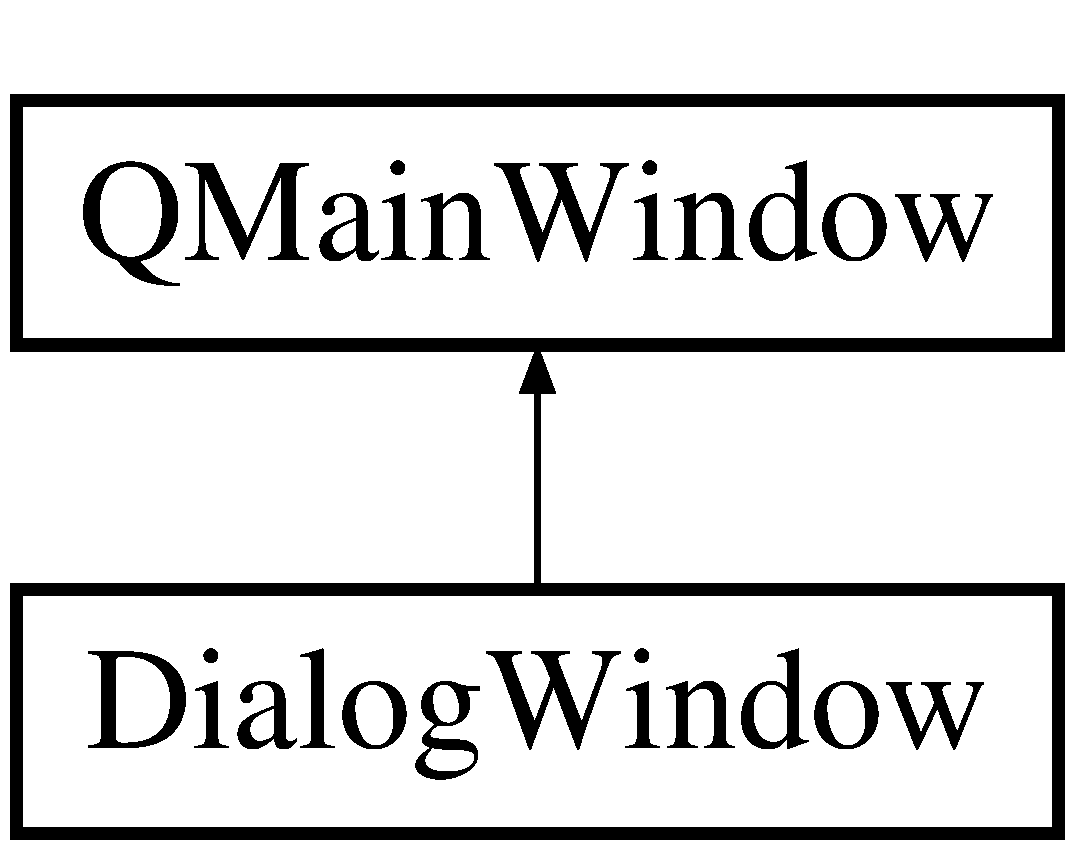
\includegraphics[height=2.000000cm]{class_dialog_window}
\end{center}
\end{figure}
\subsection*{Public Member Functions}
\begin{DoxyCompactItemize}
\item 
\hyperlink{class_dialog_window_a5947ec9e71ed3782211f6d81dd696b21}{Dialog\+Window} (Q\+Widget $\ast$parent=0)
\item 
\hyperlink{class_dialog_window_a59d3601f7622f31ef928377fc1789eda}{$\sim$\+Dialog\+Window} ()
\end{DoxyCompactItemize}
\subsection*{Protected Member Functions}
\begin{DoxyCompactItemize}
\item 
void \hyperlink{class_dialog_window_a4ebb65eafbab8384d0064ad8a0e9c6dd}{close\+Event} (Q\+Close\+Event $\ast$event) Q\+\_\+\+D\+E\+C\+L\+\_\+\+O\+V\+E\+R\+R\+I\+DE
\end{DoxyCompactItemize}
\subsection*{Private Attributes}
\begin{DoxyCompactItemize}
\item 
\hyperlink{class_ui_1_1_remote_hidden_helper_class}{Ui\+::\+Remote\+Hidden\+Helper\+Class} $\ast$ \hyperlink{class_dialog_window_ace4feb50f11737df8753b57b936d8fe2}{ui}
\end{DoxyCompactItemize}


\subsection{Detailed Description}


Definition at line 8 of file Dialog\+Window.\+h.



\subsection{Constructor \& Destructor Documentation}
\hypertarget{class_dialog_window_a5947ec9e71ed3782211f6d81dd696b21}{}\label{class_dialog_window_a5947ec9e71ed3782211f6d81dd696b21} 
\index{Dialog\+Window@{Dialog\+Window}!Dialog\+Window@{Dialog\+Window}}
\index{Dialog\+Window@{Dialog\+Window}!Dialog\+Window@{Dialog\+Window}}
\subsubsection{\texorpdfstring{Dialog\+Window()}{DialogWindow()}}
{\footnotesize\ttfamily Dialog\+Window\+::\+Dialog\+Window (\begin{DoxyParamCaption}\item[{Q\+Widget $\ast$}]{parent = {\ttfamily 0} }\end{DoxyParamCaption})\hspace{0.3cm}{\ttfamily [explicit]}}



Definition at line 5 of file Dialog\+Window.\+cpp.

\hypertarget{class_dialog_window_a59d3601f7622f31ef928377fc1789eda}{}\label{class_dialog_window_a59d3601f7622f31ef928377fc1789eda} 
\index{Dialog\+Window@{Dialog\+Window}!````~Dialog\+Window@{$\sim$\+Dialog\+Window}}
\index{````~Dialog\+Window@{$\sim$\+Dialog\+Window}!Dialog\+Window@{Dialog\+Window}}
\subsubsection{\texorpdfstring{$\sim$\+Dialog\+Window()}{~DialogWindow()}}
{\footnotesize\ttfamily Dialog\+Window\+::$\sim$\+Dialog\+Window (\begin{DoxyParamCaption}{ }\end{DoxyParamCaption})}



Definition at line 13 of file Dialog\+Window.\+cpp.



\subsection{Member Function Documentation}
\hypertarget{class_dialog_window_a4ebb65eafbab8384d0064ad8a0e9c6dd}{}\label{class_dialog_window_a4ebb65eafbab8384d0064ad8a0e9c6dd} 
\index{Dialog\+Window@{Dialog\+Window}!close\+Event@{close\+Event}}
\index{close\+Event@{close\+Event}!Dialog\+Window@{Dialog\+Window}}
\subsubsection{\texorpdfstring{close\+Event()}{closeEvent()}}
{\footnotesize\ttfamily void Dialog\+Window\+::close\+Event (\begin{DoxyParamCaption}\item[{Q\+Close\+Event $\ast$}]{event }\end{DoxyParamCaption})\hspace{0.3cm}{\ttfamily [protected]}}



Definition at line 18 of file Dialog\+Window.\+cpp.



\subsection{Member Data Documentation}
\hypertarget{class_dialog_window_ace4feb50f11737df8753b57b936d8fe2}{}\label{class_dialog_window_ace4feb50f11737df8753b57b936d8fe2} 
\index{Dialog\+Window@{Dialog\+Window}!ui@{ui}}
\index{ui@{ui}!Dialog\+Window@{Dialog\+Window}}
\subsubsection{\texorpdfstring{ui}{ui}}
{\footnotesize\ttfamily \hyperlink{class_ui_1_1_remote_hidden_helper_class}{Ui\+::\+Remote\+Hidden\+Helper\+Class}$\ast$ Dialog\+Window\+::ui\hspace{0.3cm}{\ttfamily [private]}}



Definition at line 17 of file Dialog\+Window.\+h.



The documentation for this class was generated from the following files\+:\begin{DoxyCompactItemize}
\item 
C\+:/\+Projekte/\+Remote\+Repros/\+Remote\+Hidden\+Helper/\+Remote\+Hidden\+Helper/\hyperlink{_dialog_window_8h}{Dialog\+Window.\+h}\item 
C\+:/\+Projekte/\+Remote\+Repros/\+Remote\+Hidden\+Helper/\+Remote\+Hidden\+Helper/\hyperlink{_dialog_window_8cpp}{Dialog\+Window.\+cpp}\end{DoxyCompactItemize}

\hypertarget{class_r_w_1_1_c_o_r_e_1_1_error_handler}{}\section{RW\+:\+:C\+O\+RE\+:\+:Error\+Handler Class Reference}
\label{class_r_w_1_1_c_o_r_e_1_1_error_handler}\index{R\+W\+::\+C\+O\+R\+E\+::\+Error\+Handler@{R\+W\+::\+C\+O\+R\+E\+::\+Error\+Handler}}


{\ttfamily \#include $<$Error\+Handler.\+h$>$}

Inheritance diagram for RW\+:\+:C\+O\+RE\+:\+:Error\+Handler\+:\begin{figure}[H]
\begin{center}
\leavevmode
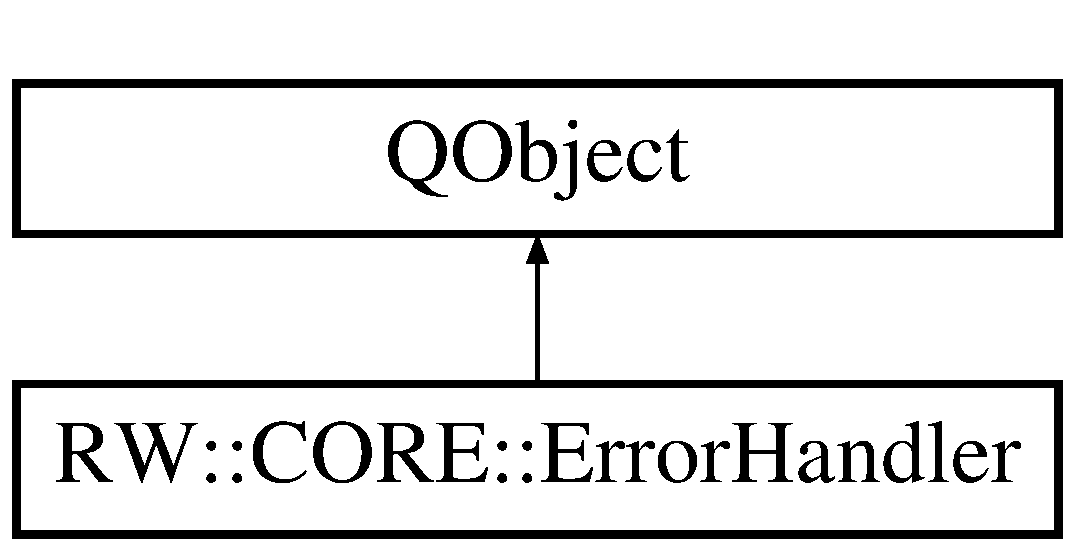
\includegraphics[height=2.000000cm]{class_r_w_1_1_c_o_r_e_1_1_error_handler}
\end{center}
\end{figure}
\subsection*{Public Slots}
\begin{DoxyCompactItemize}
\item 
void \hyperlink{class_r_w_1_1_c_o_r_e_1_1_error_handler_a7e93cff1de31d52deb41eb509730b2f0}{On\+Process\+Message\+Answer} (Util\+::\+Functions Func, Util\+::\+Error\+ID Id, Q\+Byte\+Array \hyperlink{namespace_r_w_1_1_c_o_r_e_a571834b44d0e3fab58aa6abfe5a02988}{Message})
\end{DoxyCompactItemize}
\subsection*{Signals}
\begin{DoxyCompactItemize}
\item 
void \hyperlink{class_r_w_1_1_c_o_r_e_1_1_error_handler_ad85d6dc6e06eec5d8709969600fbf059}{New\+Message} (Util\+::\+Message\+Receiver Receiver, Util\+::\+Functions Message\+Type, Q\+Byte\+Array \hyperlink{namespace_r_w_1_1_c_o_r_e_a571834b44d0e3fab58aa6abfe5a02988}{Message})
\end{DoxyCompactItemize}
\subsection*{Public Member Functions}
\begin{DoxyCompactItemize}
\item 
\hyperlink{class_r_w_1_1_c_o_r_e_1_1_error_handler_a094d83179b751152eb56cecb5548ff47}{Error\+Handler} (Q\+Object $\ast$Parent)
\item 
\hyperlink{class_r_w_1_1_c_o_r_e_1_1_error_handler_a600852f08871a018da65f523ace50bc2}{$\sim$\+Error\+Handler} ()
\item 
bool \hyperlink{class_r_w_1_1_c_o_r_e_1_1_error_handler_a63b57c30d5d7b4b2ce7c0b65ee64e627}{Is\+Busy} ()
\begin{DoxyCompactList}\small\item\em Is\+Busy zeigt an ob der \hyperlink{class_r_w_1_1_c_o_r_e_1_1_error_handler}{Error\+Handler} noch dabei ist, vorangegange Prozesse zu beenden. \end{DoxyCompactList}\item 
bool \hyperlink{class_r_w_1_1_c_o_r_e_1_1_error_handler_a43a98f148cdb6b07775e2e44a631b411}{Is\+Busy} (Util\+::\+Message\+Receiver Receiver)
\item 
void \hyperlink{class_r_w_1_1_c_o_r_e_1_1_error_handler_a1045b5b8cfce6f8476c4c61b6c797509}{Set\+Mks\+Running} (bool Running)
\item 
void \hyperlink{class_r_w_1_1_c_o_r_e_1_1_error_handler_ae068accee78e011ae187df1e05b7c9e6}{Set\+Can\+Easy\+Running} (bool Running)
\item 
void \hyperlink{class_r_w_1_1_c_o_r_e_1_1_error_handler_a838abbf533ba65c7f51266507e9d256a}{Set\+F\+Host\+Sp\+Running} (bool Running)
\end{DoxyCompactItemize}
\subsection*{Private Member Functions}
\begin{DoxyCompactItemize}
\item 
void \hyperlink{class_r_w_1_1_c_o_r_e_1_1_error_handler_a7356ddc63cc1accf1e81c7a8ebb62187}{Print\+Debug\+Information} ()
\end{DoxyCompactItemize}
\subsection*{Private Attributes}
\begin{DoxyCompactItemize}
\item 
bool \hyperlink{class_r_w_1_1_c_o_r_e_1_1_error_handler_acd15489cf612e45395d48c6054579380}{m\+\_\+\+Is\+M\+K\+S\+Running}
\item 
bool \hyperlink{class_r_w_1_1_c_o_r_e_1_1_error_handler_a430b5c523f3b9fc33d49ff3c0c440db4}{m\+\_\+\+Is\+Can\+Easy\+Running}
\item 
bool \hyperlink{class_r_w_1_1_c_o_r_e_1_1_error_handler_afbf39dd927a052468bbf9792981e73c1}{m\+\_\+\+Is\+F\+Host\+S\+P\+Running}
\end{DoxyCompactItemize}


\subsection{Detailed Description}


Definition at line 8 of file Error\+Handler.\+h.



\subsection{Constructor \& Destructor Documentation}
\hypertarget{class_r_w_1_1_c_o_r_e_1_1_error_handler_a094d83179b751152eb56cecb5548ff47}{}\label{class_r_w_1_1_c_o_r_e_1_1_error_handler_a094d83179b751152eb56cecb5548ff47} 
\index{R\+W\+::\+C\+O\+R\+E\+::\+Error\+Handler@{R\+W\+::\+C\+O\+R\+E\+::\+Error\+Handler}!Error\+Handler@{Error\+Handler}}
\index{Error\+Handler@{Error\+Handler}!R\+W\+::\+C\+O\+R\+E\+::\+Error\+Handler@{R\+W\+::\+C\+O\+R\+E\+::\+Error\+Handler}}
\subsubsection{\texorpdfstring{Error\+Handler()}{ErrorHandler()}}
{\footnotesize\ttfamily R\+W\+::\+C\+O\+R\+E\+::\+Error\+Handler\+::\+Error\+Handler (\begin{DoxyParamCaption}\item[{Q\+Object $\ast$}]{Parent }\end{DoxyParamCaption})}



Definition at line 8 of file Error\+Handler.\+cpp.

\hypertarget{class_r_w_1_1_c_o_r_e_1_1_error_handler_a600852f08871a018da65f523ace50bc2}{}\label{class_r_w_1_1_c_o_r_e_1_1_error_handler_a600852f08871a018da65f523ace50bc2} 
\index{R\+W\+::\+C\+O\+R\+E\+::\+Error\+Handler@{R\+W\+::\+C\+O\+R\+E\+::\+Error\+Handler}!````~Error\+Handler@{$\sim$\+Error\+Handler}}
\index{````~Error\+Handler@{$\sim$\+Error\+Handler}!R\+W\+::\+C\+O\+R\+E\+::\+Error\+Handler@{R\+W\+::\+C\+O\+R\+E\+::\+Error\+Handler}}
\subsubsection{\texorpdfstring{$\sim$\+Error\+Handler()}{~ErrorHandler()}}
{\footnotesize\ttfamily R\+W\+::\+C\+O\+R\+E\+::\+Error\+Handler\+::$\sim$\+Error\+Handler (\begin{DoxyParamCaption}{ }\end{DoxyParamCaption})}



Definition at line 15 of file Error\+Handler.\+cpp.



\subsection{Member Function Documentation}
\hypertarget{class_r_w_1_1_c_o_r_e_1_1_error_handler_a63b57c30d5d7b4b2ce7c0b65ee64e627}{}\label{class_r_w_1_1_c_o_r_e_1_1_error_handler_a63b57c30d5d7b4b2ce7c0b65ee64e627} 
\index{R\+W\+::\+C\+O\+R\+E\+::\+Error\+Handler@{R\+W\+::\+C\+O\+R\+E\+::\+Error\+Handler}!Is\+Busy@{Is\+Busy}}
\index{Is\+Busy@{Is\+Busy}!R\+W\+::\+C\+O\+R\+E\+::\+Error\+Handler@{R\+W\+::\+C\+O\+R\+E\+::\+Error\+Handler}}
\subsubsection{\texorpdfstring{Is\+Busy()}{IsBusy()}\hspace{0.1cm}{\footnotesize\ttfamily [1/2]}}
{\footnotesize\ttfamily bool R\+W\+::\+C\+O\+R\+E\+::\+Error\+Handler\+::\+Is\+Busy (\begin{DoxyParamCaption}{ }\end{DoxyParamCaption})\hspace{0.3cm}{\ttfamily [inline]}}



Is\+Busy zeigt an ob der \hyperlink{class_r_w_1_1_c_o_r_e_1_1_error_handler}{Error\+Handler} noch dabei ist, vorangegange Prozesse zu beenden. 



Definition at line 28 of file Error\+Handler.\+h.

\hypertarget{class_r_w_1_1_c_o_r_e_1_1_error_handler_a43a98f148cdb6b07775e2e44a631b411}{}\label{class_r_w_1_1_c_o_r_e_1_1_error_handler_a43a98f148cdb6b07775e2e44a631b411} 
\index{R\+W\+::\+C\+O\+R\+E\+::\+Error\+Handler@{R\+W\+::\+C\+O\+R\+E\+::\+Error\+Handler}!Is\+Busy@{Is\+Busy}}
\index{Is\+Busy@{Is\+Busy}!R\+W\+::\+C\+O\+R\+E\+::\+Error\+Handler@{R\+W\+::\+C\+O\+R\+E\+::\+Error\+Handler}}
\subsubsection{\texorpdfstring{Is\+Busy()}{IsBusy()}\hspace{0.1cm}{\footnotesize\ttfamily [2/2]}}
{\footnotesize\ttfamily bool R\+W\+::\+C\+O\+R\+E\+::\+Error\+Handler\+::\+Is\+Busy (\begin{DoxyParamCaption}\item[{Util\+::\+Message\+Receiver}]{Receiver }\end{DoxyParamCaption})\hspace{0.3cm}{\ttfamily [inline]}}



Definition at line 34 of file Error\+Handler.\+h.

\hypertarget{class_r_w_1_1_c_o_r_e_1_1_error_handler_ad85d6dc6e06eec5d8709969600fbf059}{}\label{class_r_w_1_1_c_o_r_e_1_1_error_handler_ad85d6dc6e06eec5d8709969600fbf059} 
\index{R\+W\+::\+C\+O\+R\+E\+::\+Error\+Handler@{R\+W\+::\+C\+O\+R\+E\+::\+Error\+Handler}!New\+Message@{New\+Message}}
\index{New\+Message@{New\+Message}!R\+W\+::\+C\+O\+R\+E\+::\+Error\+Handler@{R\+W\+::\+C\+O\+R\+E\+::\+Error\+Handler}}
\subsubsection{\texorpdfstring{New\+Message}{NewMessage}}
{\footnotesize\ttfamily void R\+W\+::\+C\+O\+R\+E\+::\+Error\+Handler\+::\+New\+Message (\begin{DoxyParamCaption}\item[{Util\+::\+Message\+Receiver}]{Receiver,  }\item[{Util\+::\+Functions}]{Message\+Type,  }\item[{Q\+Byte\+Array}]{Message }\end{DoxyParamCaption})\hspace{0.3cm}{\ttfamily [signal]}}



Definition at line 142 of file moc\+\_\+\+Error\+Handler.\+cpp.

\hypertarget{class_r_w_1_1_c_o_r_e_1_1_error_handler_a7e93cff1de31d52deb41eb509730b2f0}{}\label{class_r_w_1_1_c_o_r_e_1_1_error_handler_a7e93cff1de31d52deb41eb509730b2f0} 
\index{R\+W\+::\+C\+O\+R\+E\+::\+Error\+Handler@{R\+W\+::\+C\+O\+R\+E\+::\+Error\+Handler}!On\+Process\+Message\+Answer@{On\+Process\+Message\+Answer}}
\index{On\+Process\+Message\+Answer@{On\+Process\+Message\+Answer}!R\+W\+::\+C\+O\+R\+E\+::\+Error\+Handler@{R\+W\+::\+C\+O\+R\+E\+::\+Error\+Handler}}
\subsubsection{\texorpdfstring{On\+Process\+Message\+Answer}{OnProcessMessageAnswer}}
{\footnotesize\ttfamily void R\+W\+::\+C\+O\+R\+E\+::\+Error\+Handler\+::\+On\+Process\+Message\+Answer (\begin{DoxyParamCaption}\item[{Util\+::\+Functions}]{Func,  }\item[{Util\+::\+Error\+ID}]{Id,  }\item[{Q\+Byte\+Array}]{Message }\end{DoxyParamCaption})\hspace{0.3cm}{\ttfamily [slot]}}



Definition at line 29 of file Error\+Handler.\+cpp.

\hypertarget{class_r_w_1_1_c_o_r_e_1_1_error_handler_a7356ddc63cc1accf1e81c7a8ebb62187}{}\label{class_r_w_1_1_c_o_r_e_1_1_error_handler_a7356ddc63cc1accf1e81c7a8ebb62187} 
\index{R\+W\+::\+C\+O\+R\+E\+::\+Error\+Handler@{R\+W\+::\+C\+O\+R\+E\+::\+Error\+Handler}!Print\+Debug\+Information@{Print\+Debug\+Information}}
\index{Print\+Debug\+Information@{Print\+Debug\+Information}!R\+W\+::\+C\+O\+R\+E\+::\+Error\+Handler@{R\+W\+::\+C\+O\+R\+E\+::\+Error\+Handler}}
\subsubsection{\texorpdfstring{Print\+Debug\+Information()}{PrintDebugInformation()}}
{\footnotesize\ttfamily void R\+W\+::\+C\+O\+R\+E\+::\+Error\+Handler\+::\+Print\+Debug\+Information (\begin{DoxyParamCaption}{ }\end{DoxyParamCaption})\hspace{0.3cm}{\ttfamily [private]}}



Definition at line 19 of file Error\+Handler.\+cpp.

\hypertarget{class_r_w_1_1_c_o_r_e_1_1_error_handler_ae068accee78e011ae187df1e05b7c9e6}{}\label{class_r_w_1_1_c_o_r_e_1_1_error_handler_ae068accee78e011ae187df1e05b7c9e6} 
\index{R\+W\+::\+C\+O\+R\+E\+::\+Error\+Handler@{R\+W\+::\+C\+O\+R\+E\+::\+Error\+Handler}!Set\+Can\+Easy\+Running@{Set\+Can\+Easy\+Running}}
\index{Set\+Can\+Easy\+Running@{Set\+Can\+Easy\+Running}!R\+W\+::\+C\+O\+R\+E\+::\+Error\+Handler@{R\+W\+::\+C\+O\+R\+E\+::\+Error\+Handler}}
\subsubsection{\texorpdfstring{Set\+Can\+Easy\+Running()}{SetCanEasyRunning()}}
{\footnotesize\ttfamily void R\+W\+::\+C\+O\+R\+E\+::\+Error\+Handler\+::\+Set\+Can\+Easy\+Running (\begin{DoxyParamCaption}\item[{bool}]{Running }\end{DoxyParamCaption})\hspace{0.3cm}{\ttfamily [inline]}}



Definition at line 53 of file Error\+Handler.\+h.

\hypertarget{class_r_w_1_1_c_o_r_e_1_1_error_handler_a838abbf533ba65c7f51266507e9d256a}{}\label{class_r_w_1_1_c_o_r_e_1_1_error_handler_a838abbf533ba65c7f51266507e9d256a} 
\index{R\+W\+::\+C\+O\+R\+E\+::\+Error\+Handler@{R\+W\+::\+C\+O\+R\+E\+::\+Error\+Handler}!Set\+F\+Host\+Sp\+Running@{Set\+F\+Host\+Sp\+Running}}
\index{Set\+F\+Host\+Sp\+Running@{Set\+F\+Host\+Sp\+Running}!R\+W\+::\+C\+O\+R\+E\+::\+Error\+Handler@{R\+W\+::\+C\+O\+R\+E\+::\+Error\+Handler}}
\subsubsection{\texorpdfstring{Set\+F\+Host\+Sp\+Running()}{SetFHostSpRunning()}}
{\footnotesize\ttfamily void R\+W\+::\+C\+O\+R\+E\+::\+Error\+Handler\+::\+Set\+F\+Host\+Sp\+Running (\begin{DoxyParamCaption}\item[{bool}]{Running }\end{DoxyParamCaption})\hspace{0.3cm}{\ttfamily [inline]}}



Definition at line 54 of file Error\+Handler.\+h.

\hypertarget{class_r_w_1_1_c_o_r_e_1_1_error_handler_a1045b5b8cfce6f8476c4c61b6c797509}{}\label{class_r_w_1_1_c_o_r_e_1_1_error_handler_a1045b5b8cfce6f8476c4c61b6c797509} 
\index{R\+W\+::\+C\+O\+R\+E\+::\+Error\+Handler@{R\+W\+::\+C\+O\+R\+E\+::\+Error\+Handler}!Set\+Mks\+Running@{Set\+Mks\+Running}}
\index{Set\+Mks\+Running@{Set\+Mks\+Running}!R\+W\+::\+C\+O\+R\+E\+::\+Error\+Handler@{R\+W\+::\+C\+O\+R\+E\+::\+Error\+Handler}}
\subsubsection{\texorpdfstring{Set\+Mks\+Running()}{SetMksRunning()}}
{\footnotesize\ttfamily void R\+W\+::\+C\+O\+R\+E\+::\+Error\+Handler\+::\+Set\+Mks\+Running (\begin{DoxyParamCaption}\item[{bool}]{Running }\end{DoxyParamCaption})\hspace{0.3cm}{\ttfamily [inline]}}



Definition at line 52 of file Error\+Handler.\+h.



\subsection{Member Data Documentation}
\hypertarget{class_r_w_1_1_c_o_r_e_1_1_error_handler_a430b5c523f3b9fc33d49ff3c0c440db4}{}\label{class_r_w_1_1_c_o_r_e_1_1_error_handler_a430b5c523f3b9fc33d49ff3c0c440db4} 
\index{R\+W\+::\+C\+O\+R\+E\+::\+Error\+Handler@{R\+W\+::\+C\+O\+R\+E\+::\+Error\+Handler}!m\+\_\+\+Is\+Can\+Easy\+Running@{m\+\_\+\+Is\+Can\+Easy\+Running}}
\index{m\+\_\+\+Is\+Can\+Easy\+Running@{m\+\_\+\+Is\+Can\+Easy\+Running}!R\+W\+::\+C\+O\+R\+E\+::\+Error\+Handler@{R\+W\+::\+C\+O\+R\+E\+::\+Error\+Handler}}
\subsubsection{\texorpdfstring{m\+\_\+\+Is\+Can\+Easy\+Running}{m\_IsCanEasyRunning}}
{\footnotesize\ttfamily bool R\+W\+::\+C\+O\+R\+E\+::\+Error\+Handler\+::m\+\_\+\+Is\+Can\+Easy\+Running\hspace{0.3cm}{\ttfamily [private]}}



Definition at line 15 of file Error\+Handler.\+h.

\hypertarget{class_r_w_1_1_c_o_r_e_1_1_error_handler_afbf39dd927a052468bbf9792981e73c1}{}\label{class_r_w_1_1_c_o_r_e_1_1_error_handler_afbf39dd927a052468bbf9792981e73c1} 
\index{R\+W\+::\+C\+O\+R\+E\+::\+Error\+Handler@{R\+W\+::\+C\+O\+R\+E\+::\+Error\+Handler}!m\+\_\+\+Is\+F\+Host\+S\+P\+Running@{m\+\_\+\+Is\+F\+Host\+S\+P\+Running}}
\index{m\+\_\+\+Is\+F\+Host\+S\+P\+Running@{m\+\_\+\+Is\+F\+Host\+S\+P\+Running}!R\+W\+::\+C\+O\+R\+E\+::\+Error\+Handler@{R\+W\+::\+C\+O\+R\+E\+::\+Error\+Handler}}
\subsubsection{\texorpdfstring{m\+\_\+\+Is\+F\+Host\+S\+P\+Running}{m\_IsFHostSPRunning}}
{\footnotesize\ttfamily bool R\+W\+::\+C\+O\+R\+E\+::\+Error\+Handler\+::m\+\_\+\+Is\+F\+Host\+S\+P\+Running\hspace{0.3cm}{\ttfamily [private]}}



Definition at line 16 of file Error\+Handler.\+h.

\hypertarget{class_r_w_1_1_c_o_r_e_1_1_error_handler_acd15489cf612e45395d48c6054579380}{}\label{class_r_w_1_1_c_o_r_e_1_1_error_handler_acd15489cf612e45395d48c6054579380} 
\index{R\+W\+::\+C\+O\+R\+E\+::\+Error\+Handler@{R\+W\+::\+C\+O\+R\+E\+::\+Error\+Handler}!m\+\_\+\+Is\+M\+K\+S\+Running@{m\+\_\+\+Is\+M\+K\+S\+Running}}
\index{m\+\_\+\+Is\+M\+K\+S\+Running@{m\+\_\+\+Is\+M\+K\+S\+Running}!R\+W\+::\+C\+O\+R\+E\+::\+Error\+Handler@{R\+W\+::\+C\+O\+R\+E\+::\+Error\+Handler}}
\subsubsection{\texorpdfstring{m\+\_\+\+Is\+M\+K\+S\+Running}{m\_IsMKSRunning}}
{\footnotesize\ttfamily bool R\+W\+::\+C\+O\+R\+E\+::\+Error\+Handler\+::m\+\_\+\+Is\+M\+K\+S\+Running\hspace{0.3cm}{\ttfamily [private]}}



Definition at line 14 of file Error\+Handler.\+h.



The documentation for this class was generated from the following files\+:\begin{DoxyCompactItemize}
\item 
C\+:/\+Projekte/\+Remote\+Repros/\+Remote\+Hidden\+Helper/\+Remote\+Hidden\+Helper/\hyperlink{_error_handler_8h}{Error\+Handler.\+h}\item 
C\+:/\+Projekte/\+Remote\+Repros/\+Remote\+Hidden\+Helper/\+Remote\+Hidden\+Helper/\hyperlink{_error_handler_8cpp}{Error\+Handler.\+cpp}\item 
C\+:/\+Projekte/\+Remote\+Repros/\+Remote\+Hidden\+Helper/\+Remote\+Hidden\+Helper/\+Generated\+Files/\+Debug/\hyperlink{moc___error_handler_8cpp}{moc\+\_\+\+Error\+Handler.\+cpp}\end{DoxyCompactItemize}

\hypertarget{class_r_w_1_1_c_o_r_e_1_1_f_host_sp_wrapper}{}\section{RW\+:\+:C\+O\+RE\+:\+:F\+Host\+Sp\+Wrapper Class Reference}
\label{class_r_w_1_1_c_o_r_e_1_1_f_host_sp_wrapper}\index{R\+W\+::\+C\+O\+R\+E\+::\+F\+Host\+Sp\+Wrapper@{R\+W\+::\+C\+O\+R\+E\+::\+F\+Host\+Sp\+Wrapper}}


{\ttfamily \#include $<$F\+Host\+Sp\+Wrapper.\+h$>$}

Inheritance diagram for RW\+:\+:C\+O\+RE\+:\+:F\+Host\+Sp\+Wrapper\+:\begin{figure}[H]
\begin{center}
\leavevmode
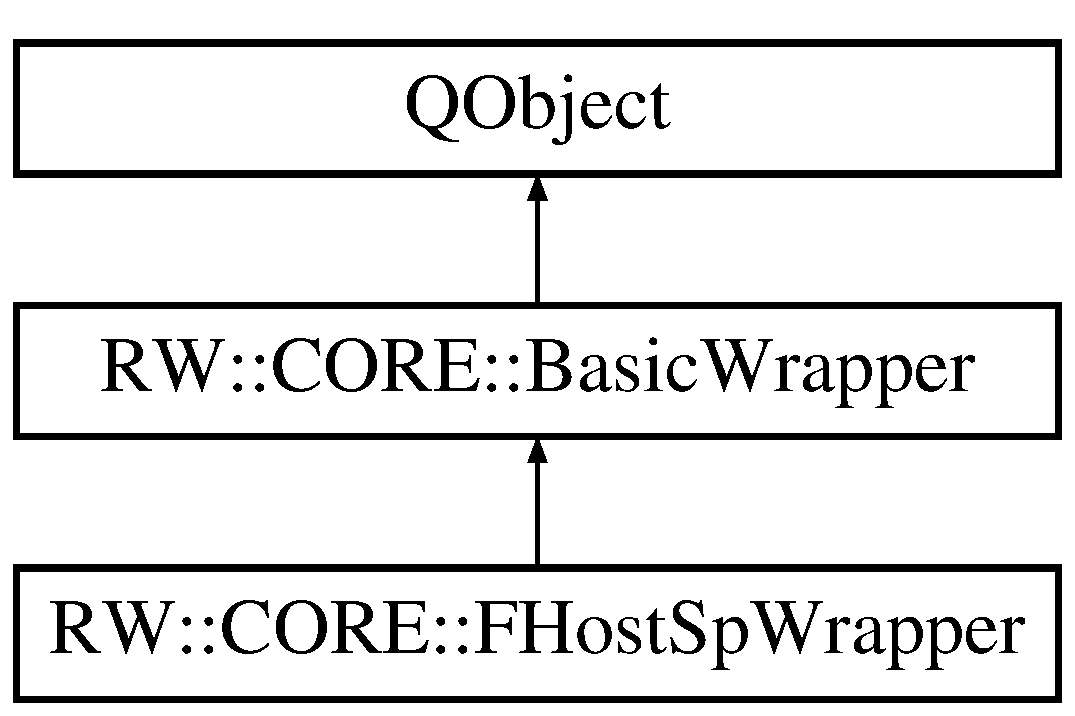
\includegraphics[height=3.000000cm]{class_r_w_1_1_c_o_r_e_1_1_f_host_sp_wrapper}
\end{center}
\end{figure}
\subsection*{Public Slots}
\begin{DoxyCompactItemize}
\item 
void \hyperlink{class_r_w_1_1_c_o_r_e_1_1_f_host_sp_wrapper_a60128d89802ee6ded357d3bfee856625}{On\+Process\+Message} (Util\+::\+Message\+Receiver Type, Util\+::\+Functions Func, Q\+Byte\+Array Report)
\end{DoxyCompactItemize}
\subsection*{Public Member Functions}
\begin{DoxyCompactItemize}
\item 
\hyperlink{class_r_w_1_1_c_o_r_e_1_1_f_host_sp_wrapper_ae333b04fe313284ac0a4a7b872e31b83}{F\+Host\+Sp\+Wrapper} (Q\+Object $\ast$Parent=nullptr)
\item 
\hyperlink{class_r_w_1_1_c_o_r_e_1_1_f_host_sp_wrapper_a5d596866de0091d77fbcab7fb557faae}{$\sim$\+F\+Host\+Sp\+Wrapper} ()
\item 
void \hyperlink{class_r_w_1_1_c_o_r_e_1_1_f_host_sp_wrapper_ad2daebbd1b0140480d03b31916cd6c35}{Start\+F\+Host\+SP} ()
\item 
void \hyperlink{class_r_w_1_1_c_o_r_e_1_1_f_host_sp_wrapper_abfbe1c65f2383e10da83dfd1ab5825f0}{Close\+Sequence} ()
\item 
void \hyperlink{class_r_w_1_1_c_o_r_e_1_1_f_host_sp_wrapper_ad586b9e7711a788688322ee7d54b0320}{Get\+Progress} ()
\item 
void \hyperlink{class_r_w_1_1_c_o_r_e_1_1_f_host_sp_wrapper_a00ff512e1699742a7908540c11be1e40}{Close\+Application} ()
\item 
void \hyperlink{class_r_w_1_1_c_o_r_e_1_1_f_host_sp_wrapper_ad173aae317d00608bc92d826e5befe64}{Get\+State} ()
\item 
void \hyperlink{class_r_w_1_1_c_o_r_e_1_1_f_host_sp_wrapper_ad95d9017361d78c466afaf3c2bd391ee}{Abort\+Sequence} ()
\item 
void \hyperlink{class_r_w_1_1_c_o_r_e_1_1_f_host_sp_wrapper_a5d384a433b333b1f5f7b7465ad138d4c}{Load\+Sequence} (const Q\+File \&Flashfile)
\item 
void \hyperlink{class_r_w_1_1_c_o_r_e_1_1_f_host_sp_wrapper_a718318bc9b98f97ff311f8174adfb172}{Start\+Sequence} ()
\end{DoxyCompactItemize}
\subsection*{Private Attributes}
\begin{DoxyCompactItemize}
\item 
C\+Com\+Ptr$<$ I\+F\+Host\+S\+P\+\_\+\+Remote\+Interface $>$ \hyperlink{class_r_w_1_1_c_o_r_e_1_1_f_host_sp_wrapper_a85c312c5d8288140d1d2a31fd15946a9}{m\+\_\+\+Process}
\item 
std\+::string \hyperlink{class_r_w_1_1_c_o_r_e_1_1_f_host_sp_wrapper_a3760e496eac5633321be3f2345b86b88}{m\+\_\+\+Workspace\+Path}
\end{DoxyCompactItemize}
\subsection*{Additional Inherited Members}


\subsection{Detailed Description}


Definition at line 10 of file F\+Host\+Sp\+Wrapper.\+h.



\subsection{Constructor \& Destructor Documentation}
\hypertarget{class_r_w_1_1_c_o_r_e_1_1_f_host_sp_wrapper_ae333b04fe313284ac0a4a7b872e31b83}{}\label{class_r_w_1_1_c_o_r_e_1_1_f_host_sp_wrapper_ae333b04fe313284ac0a4a7b872e31b83} 
\index{R\+W\+::\+C\+O\+R\+E\+::\+F\+Host\+Sp\+Wrapper@{R\+W\+::\+C\+O\+R\+E\+::\+F\+Host\+Sp\+Wrapper}!F\+Host\+Sp\+Wrapper@{F\+Host\+Sp\+Wrapper}}
\index{F\+Host\+Sp\+Wrapper@{F\+Host\+Sp\+Wrapper}!R\+W\+::\+C\+O\+R\+E\+::\+F\+Host\+Sp\+Wrapper@{R\+W\+::\+C\+O\+R\+E\+::\+F\+Host\+Sp\+Wrapper}}
\subsubsection{\texorpdfstring{F\+Host\+Sp\+Wrapper()}{FHostSpWrapper()}}
{\footnotesize\ttfamily R\+W\+::\+C\+O\+R\+E\+::\+F\+Host\+Sp\+Wrapper\+::\+F\+Host\+Sp\+Wrapper (\begin{DoxyParamCaption}\item[{Q\+Object $\ast$}]{Parent = {\ttfamily nullptr} }\end{DoxyParamCaption})}



Definition at line 13 of file F\+Host\+Sp\+Wrapper.\+cpp.

\hypertarget{class_r_w_1_1_c_o_r_e_1_1_f_host_sp_wrapper_a5d596866de0091d77fbcab7fb557faae}{}\label{class_r_w_1_1_c_o_r_e_1_1_f_host_sp_wrapper_a5d596866de0091d77fbcab7fb557faae} 
\index{R\+W\+::\+C\+O\+R\+E\+::\+F\+Host\+Sp\+Wrapper@{R\+W\+::\+C\+O\+R\+E\+::\+F\+Host\+Sp\+Wrapper}!````~F\+Host\+Sp\+Wrapper@{$\sim$\+F\+Host\+Sp\+Wrapper}}
\index{````~F\+Host\+Sp\+Wrapper@{$\sim$\+F\+Host\+Sp\+Wrapper}!R\+W\+::\+C\+O\+R\+E\+::\+F\+Host\+Sp\+Wrapper@{R\+W\+::\+C\+O\+R\+E\+::\+F\+Host\+Sp\+Wrapper}}
\subsubsection{\texorpdfstring{$\sim$\+F\+Host\+Sp\+Wrapper()}{~FHostSpWrapper()}}
{\footnotesize\ttfamily R\+W\+::\+C\+O\+R\+E\+::\+F\+Host\+Sp\+Wrapper\+::$\sim$\+F\+Host\+Sp\+Wrapper (\begin{DoxyParamCaption}{ }\end{DoxyParamCaption})}



Definition at line 18 of file F\+Host\+Sp\+Wrapper.\+cpp.



\subsection{Member Function Documentation}
\hypertarget{class_r_w_1_1_c_o_r_e_1_1_f_host_sp_wrapper_ad95d9017361d78c466afaf3c2bd391ee}{}\label{class_r_w_1_1_c_o_r_e_1_1_f_host_sp_wrapper_ad95d9017361d78c466afaf3c2bd391ee} 
\index{R\+W\+::\+C\+O\+R\+E\+::\+F\+Host\+Sp\+Wrapper@{R\+W\+::\+C\+O\+R\+E\+::\+F\+Host\+Sp\+Wrapper}!Abort\+Sequence@{Abort\+Sequence}}
\index{Abort\+Sequence@{Abort\+Sequence}!R\+W\+::\+C\+O\+R\+E\+::\+F\+Host\+Sp\+Wrapper@{R\+W\+::\+C\+O\+R\+E\+::\+F\+Host\+Sp\+Wrapper}}
\subsubsection{\texorpdfstring{Abort\+Sequence()}{AbortSequence()}}
{\footnotesize\ttfamily void R\+W\+::\+C\+O\+R\+E\+::\+F\+Host\+Sp\+Wrapper\+::\+Abort\+Sequence (\begin{DoxyParamCaption}{ }\end{DoxyParamCaption})}



Definition at line 129 of file F\+Host\+Sp\+Wrapper.\+cpp.

\hypertarget{class_r_w_1_1_c_o_r_e_1_1_f_host_sp_wrapper_a00ff512e1699742a7908540c11be1e40}{}\label{class_r_w_1_1_c_o_r_e_1_1_f_host_sp_wrapper_a00ff512e1699742a7908540c11be1e40} 
\index{R\+W\+::\+C\+O\+R\+E\+::\+F\+Host\+Sp\+Wrapper@{R\+W\+::\+C\+O\+R\+E\+::\+F\+Host\+Sp\+Wrapper}!Close\+Application@{Close\+Application}}
\index{Close\+Application@{Close\+Application}!R\+W\+::\+C\+O\+R\+E\+::\+F\+Host\+Sp\+Wrapper@{R\+W\+::\+C\+O\+R\+E\+::\+F\+Host\+Sp\+Wrapper}}
\subsubsection{\texorpdfstring{Close\+Application()}{CloseApplication()}}
{\footnotesize\ttfamily void R\+W\+::\+C\+O\+R\+E\+::\+F\+Host\+Sp\+Wrapper\+::\+Close\+Application (\begin{DoxyParamCaption}{ }\end{DoxyParamCaption})}



Definition at line 100 of file F\+Host\+Sp\+Wrapper.\+cpp.

\hypertarget{class_r_w_1_1_c_o_r_e_1_1_f_host_sp_wrapper_abfbe1c65f2383e10da83dfd1ab5825f0}{}\label{class_r_w_1_1_c_o_r_e_1_1_f_host_sp_wrapper_abfbe1c65f2383e10da83dfd1ab5825f0} 
\index{R\+W\+::\+C\+O\+R\+E\+::\+F\+Host\+Sp\+Wrapper@{R\+W\+::\+C\+O\+R\+E\+::\+F\+Host\+Sp\+Wrapper}!Close\+Sequence@{Close\+Sequence}}
\index{Close\+Sequence@{Close\+Sequence}!R\+W\+::\+C\+O\+R\+E\+::\+F\+Host\+Sp\+Wrapper@{R\+W\+::\+C\+O\+R\+E\+::\+F\+Host\+Sp\+Wrapper}}
\subsubsection{\texorpdfstring{Close\+Sequence()}{CloseSequence()}}
{\footnotesize\ttfamily void R\+W\+::\+C\+O\+R\+E\+::\+F\+Host\+Sp\+Wrapper\+::\+Close\+Sequence (\begin{DoxyParamCaption}{ }\end{DoxyParamCaption})}



Definition at line 75 of file F\+Host\+Sp\+Wrapper.\+cpp.

\hypertarget{class_r_w_1_1_c_o_r_e_1_1_f_host_sp_wrapper_ad586b9e7711a788688322ee7d54b0320}{}\label{class_r_w_1_1_c_o_r_e_1_1_f_host_sp_wrapper_ad586b9e7711a788688322ee7d54b0320} 
\index{R\+W\+::\+C\+O\+R\+E\+::\+F\+Host\+Sp\+Wrapper@{R\+W\+::\+C\+O\+R\+E\+::\+F\+Host\+Sp\+Wrapper}!Get\+Progress@{Get\+Progress}}
\index{Get\+Progress@{Get\+Progress}!R\+W\+::\+C\+O\+R\+E\+::\+F\+Host\+Sp\+Wrapper@{R\+W\+::\+C\+O\+R\+E\+::\+F\+Host\+Sp\+Wrapper}}
\subsubsection{\texorpdfstring{Get\+Progress()}{GetProgress()}}
{\footnotesize\ttfamily void R\+W\+::\+C\+O\+R\+E\+::\+F\+Host\+Sp\+Wrapper\+::\+Get\+Progress (\begin{DoxyParamCaption}{ }\end{DoxyParamCaption})}



Definition at line 86 of file F\+Host\+Sp\+Wrapper.\+cpp.

\hypertarget{class_r_w_1_1_c_o_r_e_1_1_f_host_sp_wrapper_ad173aae317d00608bc92d826e5befe64}{}\label{class_r_w_1_1_c_o_r_e_1_1_f_host_sp_wrapper_ad173aae317d00608bc92d826e5befe64} 
\index{R\+W\+::\+C\+O\+R\+E\+::\+F\+Host\+Sp\+Wrapper@{R\+W\+::\+C\+O\+R\+E\+::\+F\+Host\+Sp\+Wrapper}!Get\+State@{Get\+State}}
\index{Get\+State@{Get\+State}!R\+W\+::\+C\+O\+R\+E\+::\+F\+Host\+Sp\+Wrapper@{R\+W\+::\+C\+O\+R\+E\+::\+F\+Host\+Sp\+Wrapper}}
\subsubsection{\texorpdfstring{Get\+State()}{GetState()}}
{\footnotesize\ttfamily void R\+W\+::\+C\+O\+R\+E\+::\+F\+Host\+Sp\+Wrapper\+::\+Get\+State (\begin{DoxyParamCaption}{ }\end{DoxyParamCaption})}



Definition at line 111 of file F\+Host\+Sp\+Wrapper.\+cpp.

\hypertarget{class_r_w_1_1_c_o_r_e_1_1_f_host_sp_wrapper_a5d384a433b333b1f5f7b7465ad138d4c}{}\label{class_r_w_1_1_c_o_r_e_1_1_f_host_sp_wrapper_a5d384a433b333b1f5f7b7465ad138d4c} 
\index{R\+W\+::\+C\+O\+R\+E\+::\+F\+Host\+Sp\+Wrapper@{R\+W\+::\+C\+O\+R\+E\+::\+F\+Host\+Sp\+Wrapper}!Load\+Sequence@{Load\+Sequence}}
\index{Load\+Sequence@{Load\+Sequence}!R\+W\+::\+C\+O\+R\+E\+::\+F\+Host\+Sp\+Wrapper@{R\+W\+::\+C\+O\+R\+E\+::\+F\+Host\+Sp\+Wrapper}}
\subsubsection{\texorpdfstring{Load\+Sequence()}{LoadSequence()}}
{\footnotesize\ttfamily void R\+W\+::\+C\+O\+R\+E\+::\+F\+Host\+Sp\+Wrapper\+::\+Load\+Sequence (\begin{DoxyParamCaption}\item[{const Q\+File \&}]{Flashfile }\end{DoxyParamCaption})}



Definition at line 142 of file F\+Host\+Sp\+Wrapper.\+cpp.

\hypertarget{class_r_w_1_1_c_o_r_e_1_1_f_host_sp_wrapper_a60128d89802ee6ded357d3bfee856625}{}\label{class_r_w_1_1_c_o_r_e_1_1_f_host_sp_wrapper_a60128d89802ee6ded357d3bfee856625} 
\index{R\+W\+::\+C\+O\+R\+E\+::\+F\+Host\+Sp\+Wrapper@{R\+W\+::\+C\+O\+R\+E\+::\+F\+Host\+Sp\+Wrapper}!On\+Process\+Message@{On\+Process\+Message}}
\index{On\+Process\+Message@{On\+Process\+Message}!R\+W\+::\+C\+O\+R\+E\+::\+F\+Host\+Sp\+Wrapper@{R\+W\+::\+C\+O\+R\+E\+::\+F\+Host\+Sp\+Wrapper}}
\subsubsection{\texorpdfstring{On\+Process\+Message}{OnProcessMessage}}
{\footnotesize\ttfamily void R\+W\+::\+C\+O\+R\+E\+::\+F\+Host\+Sp\+Wrapper\+::\+On\+Process\+Message (\begin{DoxyParamCaption}\item[{Util\+::\+Message\+Receiver}]{Type,  }\item[{Util\+::\+Functions}]{Func,  }\item[{Q\+Byte\+Array}]{Report }\end{DoxyParamCaption})\hspace{0.3cm}{\ttfamily [slot]}}



Definition at line 22 of file F\+Host\+Sp\+Wrapper.\+cpp.

\hypertarget{class_r_w_1_1_c_o_r_e_1_1_f_host_sp_wrapper_ad2daebbd1b0140480d03b31916cd6c35}{}\label{class_r_w_1_1_c_o_r_e_1_1_f_host_sp_wrapper_ad2daebbd1b0140480d03b31916cd6c35} 
\index{R\+W\+::\+C\+O\+R\+E\+::\+F\+Host\+Sp\+Wrapper@{R\+W\+::\+C\+O\+R\+E\+::\+F\+Host\+Sp\+Wrapper}!Start\+F\+Host\+SP@{Start\+F\+Host\+SP}}
\index{Start\+F\+Host\+SP@{Start\+F\+Host\+SP}!R\+W\+::\+C\+O\+R\+E\+::\+F\+Host\+Sp\+Wrapper@{R\+W\+::\+C\+O\+R\+E\+::\+F\+Host\+Sp\+Wrapper}}
\subsubsection{\texorpdfstring{Start\+F\+Host\+S\+P()}{StartFHostSP()}}
{\footnotesize\ttfamily void R\+W\+::\+C\+O\+R\+E\+::\+F\+Host\+Sp\+Wrapper\+::\+Start\+F\+Host\+SP (\begin{DoxyParamCaption}{ }\end{DoxyParamCaption})}



Definition at line 61 of file F\+Host\+Sp\+Wrapper.\+cpp.

\hypertarget{class_r_w_1_1_c_o_r_e_1_1_f_host_sp_wrapper_a718318bc9b98f97ff311f8174adfb172}{}\label{class_r_w_1_1_c_o_r_e_1_1_f_host_sp_wrapper_a718318bc9b98f97ff311f8174adfb172} 
\index{R\+W\+::\+C\+O\+R\+E\+::\+F\+Host\+Sp\+Wrapper@{R\+W\+::\+C\+O\+R\+E\+::\+F\+Host\+Sp\+Wrapper}!Start\+Sequence@{Start\+Sequence}}
\index{Start\+Sequence@{Start\+Sequence}!R\+W\+::\+C\+O\+R\+E\+::\+F\+Host\+Sp\+Wrapper@{R\+W\+::\+C\+O\+R\+E\+::\+F\+Host\+Sp\+Wrapper}}
\subsubsection{\texorpdfstring{Start\+Sequence()}{StartSequence()}}
{\footnotesize\ttfamily void R\+W\+::\+C\+O\+R\+E\+::\+F\+Host\+Sp\+Wrapper\+::\+Start\+Sequence (\begin{DoxyParamCaption}{ }\end{DoxyParamCaption})}



Definition at line 188 of file F\+Host\+Sp\+Wrapper.\+cpp.



\subsection{Member Data Documentation}
\hypertarget{class_r_w_1_1_c_o_r_e_1_1_f_host_sp_wrapper_a85c312c5d8288140d1d2a31fd15946a9}{}\label{class_r_w_1_1_c_o_r_e_1_1_f_host_sp_wrapper_a85c312c5d8288140d1d2a31fd15946a9} 
\index{R\+W\+::\+C\+O\+R\+E\+::\+F\+Host\+Sp\+Wrapper@{R\+W\+::\+C\+O\+R\+E\+::\+F\+Host\+Sp\+Wrapper}!m\+\_\+\+Process@{m\+\_\+\+Process}}
\index{m\+\_\+\+Process@{m\+\_\+\+Process}!R\+W\+::\+C\+O\+R\+E\+::\+F\+Host\+Sp\+Wrapper@{R\+W\+::\+C\+O\+R\+E\+::\+F\+Host\+Sp\+Wrapper}}
\subsubsection{\texorpdfstring{m\+\_\+\+Process}{m\_Process}}
{\footnotesize\ttfamily C\+Com\+Ptr$<$I\+F\+Host\+S\+P\+\_\+\+Remote\+Interface$>$ R\+W\+::\+C\+O\+R\+E\+::\+F\+Host\+Sp\+Wrapper\+::m\+\_\+\+Process\hspace{0.3cm}{\ttfamily [private]}}



Definition at line 15 of file F\+Host\+Sp\+Wrapper.\+h.

\hypertarget{class_r_w_1_1_c_o_r_e_1_1_f_host_sp_wrapper_a3760e496eac5633321be3f2345b86b88}{}\label{class_r_w_1_1_c_o_r_e_1_1_f_host_sp_wrapper_a3760e496eac5633321be3f2345b86b88} 
\index{R\+W\+::\+C\+O\+R\+E\+::\+F\+Host\+Sp\+Wrapper@{R\+W\+::\+C\+O\+R\+E\+::\+F\+Host\+Sp\+Wrapper}!m\+\_\+\+Workspace\+Path@{m\+\_\+\+Workspace\+Path}}
\index{m\+\_\+\+Workspace\+Path@{m\+\_\+\+Workspace\+Path}!R\+W\+::\+C\+O\+R\+E\+::\+F\+Host\+Sp\+Wrapper@{R\+W\+::\+C\+O\+R\+E\+::\+F\+Host\+Sp\+Wrapper}}
\subsubsection{\texorpdfstring{m\+\_\+\+Workspace\+Path}{m\_WorkspacePath}}
{\footnotesize\ttfamily std\+::string R\+W\+::\+C\+O\+R\+E\+::\+F\+Host\+Sp\+Wrapper\+::m\+\_\+\+Workspace\+Path\hspace{0.3cm}{\ttfamily [private]}}



Definition at line 16 of file F\+Host\+Sp\+Wrapper.\+h.



The documentation for this class was generated from the following files\+:\begin{DoxyCompactItemize}
\item 
C\+:/\+Projekte/\+Remote\+Repros/\+Remote\+Hidden\+Helper/\+Remote\+Hidden\+Helper/\hyperlink{_f_host_sp_wrapper_8h}{F\+Host\+Sp\+Wrapper.\+h}\item 
C\+:/\+Projekte/\+Remote\+Repros/\+Remote\+Hidden\+Helper/\+Remote\+Hidden\+Helper/\hyperlink{_f_host_sp_wrapper_8cpp}{F\+Host\+Sp\+Wrapper.\+cpp}\end{DoxyCompactItemize}

\hypertarget{class_r_w_1_1_c_o_r_e_1_1_flash_informations}{}\section{RW\+:\+:C\+O\+RE\+:\+:Flash\+Informations Class Reference}
\label{class_r_w_1_1_c_o_r_e_1_1_flash_informations}\index{R\+W\+::\+C\+O\+R\+E\+::\+Flash\+Informations@{R\+W\+::\+C\+O\+R\+E\+::\+Flash\+Informations}}


{\ttfamily \#include $<$Flash\+Informations.\+h$>$}

Inheritance diagram for RW\+:\+:C\+O\+RE\+:\+:Flash\+Informations\+:\begin{figure}[H]
\begin{center}
\leavevmode
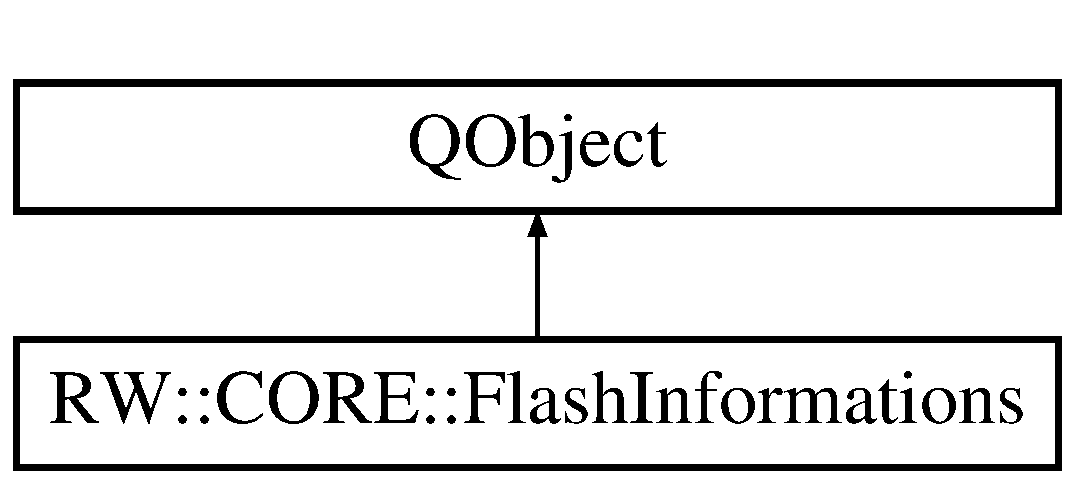
\includegraphics[height=2.000000cm]{class_r_w_1_1_c_o_r_e_1_1_flash_informations}
\end{center}
\end{figure}
\subsection*{Public Member Functions}
\begin{DoxyCompactItemize}
\item 
\hyperlink{class_r_w_1_1_c_o_r_e_1_1_flash_informations_a4633cccd76bbe9dd83d59b364c5d05f8}{Flash\+Informations} (Q\+Object $\ast$Parent=nullptr)
\item 
\hyperlink{class_r_w_1_1_c_o_r_e_1_1_flash_informations_ac734d4d58ff3dea7dcdc5c7be4a9f7b6}{$\sim$\+Flash\+Informations} ()
\item 
Q\+String\+List \hyperlink{class_r_w_1_1_c_o_r_e_1_1_flash_informations_a54957a74376f4d9481b6e4a72ebd5aa9}{Get\+Software\+By\+Id} (int system\+Id, bool AC, bool GC)
\item 
Util\+::\+Error\+ID \hyperlink{class_r_w_1_1_c_o_r_e_1_1_flash_informations_aa811fbcf9e0267f0d211d92a0b359c32}{Get\+Unique\+Keys} (Q\+List$<$ Q\+String $>$ \&Unique\+Projects)
\item 
Util\+::\+Error\+ID \hyperlink{class_r_w_1_1_c_o_r_e_1_1_flash_informations_a0be370348f9ae51c37d7af7d4a6a660d}{Get\+Sample\+Phase\+List} (Q\+String Selected\+Project, Q\+List$<$ Q\+String $>$ \&Unique\+Sample\+Phase)
\item 
Util\+::\+Error\+ID \hyperlink{class_r_w_1_1_c_o_r_e_1_1_flash_informations_affbc5dd5c41a1417a33ec5490d2b1875}{Get\+Release\+List} (Q\+String Selected\+Sample\+Phase, Q\+String Selected\+Projec, Q\+List$<$ Q\+String $>$ \&Unique\+Release\+List)
\item 
quint16 \hyperlink{class_r_w_1_1_c_o_r_e_1_1_flash_informations_a033177c5ea7b1b56ca7eac10f781c80b}{Get\+Software\+ID} (Q\+String Project\+Main, Q\+String Samplephase, Q\+String Release, Q\+String Project\+Conttroller, Q\+String Project\+Variant, Q\+String Project\+Modell\+Year)
\end{DoxyCompactItemize}
\subsection*{Private Member Functions}
\begin{DoxyCompactItemize}
\item 
Q\+String \hyperlink{class_r_w_1_1_c_o_r_e_1_1_flash_informations_a54a1ad5f711dd80d570e1d93ae205bd3}{Get\+Fitting\+Ac\+By\+Git\+Hash} (Q\+String hash)
\item 
Q\+String \hyperlink{class_r_w_1_1_c_o_r_e_1_1_flash_informations_a55b9f9803354a19f3f43e21590389a64}{Get\+Ac\+By\+Icom} (uint checksum)
\item 
Q\+String \hyperlink{class_r_w_1_1_c_o_r_e_1_1_flash_informations_a3821e59e8bab2cbef251fc05fa070811}{Get\+Releases} ()
\item 
Q\+String \hyperlink{class_r_w_1_1_c_o_r_e_1_1_flash_informations_a1584d6557b93628bc86db88af13d0d4b}{Web\+Request} (Q\+Network\+Request \&Request)
\item 
Util\+::\+Error\+ID \hyperlink{class_r_w_1_1_c_o_r_e_1_1_flash_informations_a80c0651369e180838543d0f125aa56ef}{Fill\+Release\+Map} ()
\item 
void \hyperlink{class_r_w_1_1_c_o_r_e_1_1_flash_informations_aa637abd5665ab3253c28b2f56552df4a}{Prepare\+Project\+Information} ()
\item 
Util\+::\+Error\+ID \hyperlink{class_r_w_1_1_c_o_r_e_1_1_flash_informations_acfe7f2e69b85b4a62b7dff2bd2131049}{Prepare\+Sample\+Phase\+Information} (Q\+String Selected\+Project, Q\+List$<$ Q\+String $>$ \&Unique\+Sample\+Phase)
\item 
Util\+::\+Error\+ID \hyperlink{class_r_w_1_1_c_o_r_e_1_1_flash_informations_a02e53be6cd2fddc476129dde406ca241}{Prepare\+Release\+Information} (Q\+String Selected\+Sample\+Phase, Q\+String Selected\+Project, Q\+List$<$ Q\+String $>$ \&Unique\+Release\+List)
\end{DoxyCompactItemize}
\subsection*{Private Attributes}
\begin{DoxyCompactItemize}
\item 
Q\+Multi\+Map$<$ Q\+String, Q\+String $>$ $\ast$ \hyperlink{class_r_w_1_1_c_o_r_e_1_1_flash_informations_a710529bd946b8189fae80e14c1c74599}{m\+\_\+\+Release\+Map}
\item 
Q\+String\+List \hyperlink{class_r_w_1_1_c_o_r_e_1_1_flash_informations_a03b8c748a630e47e5310ba4bbd8bd3fa}{m\+\_\+\+Release\+Buffer}
\end{DoxyCompactItemize}


\subsection{Detailed Description}


Definition at line 12 of file Flash\+Informations.\+h.



\subsection{Constructor \& Destructor Documentation}
\hypertarget{class_r_w_1_1_c_o_r_e_1_1_flash_informations_a4633cccd76bbe9dd83d59b364c5d05f8}{}\label{class_r_w_1_1_c_o_r_e_1_1_flash_informations_a4633cccd76bbe9dd83d59b364c5d05f8} 
\index{R\+W\+::\+C\+O\+R\+E\+::\+Flash\+Informations@{R\+W\+::\+C\+O\+R\+E\+::\+Flash\+Informations}!Flash\+Informations@{Flash\+Informations}}
\index{Flash\+Informations@{Flash\+Informations}!R\+W\+::\+C\+O\+R\+E\+::\+Flash\+Informations@{R\+W\+::\+C\+O\+R\+E\+::\+Flash\+Informations}}
\subsubsection{\texorpdfstring{Flash\+Informations()}{FlashInformations()}}
{\footnotesize\ttfamily R\+W\+::\+C\+O\+R\+E\+::\+Flash\+Informations\+::\+Flash\+Informations (\begin{DoxyParamCaption}\item[{Q\+Object $\ast$}]{Parent = {\ttfamily nullptr} }\end{DoxyParamCaption})}



Definition at line 35 of file Flash\+Informations.\+cpp.

\hypertarget{class_r_w_1_1_c_o_r_e_1_1_flash_informations_ac734d4d58ff3dea7dcdc5c7be4a9f7b6}{}\label{class_r_w_1_1_c_o_r_e_1_1_flash_informations_ac734d4d58ff3dea7dcdc5c7be4a9f7b6} 
\index{R\+W\+::\+C\+O\+R\+E\+::\+Flash\+Informations@{R\+W\+::\+C\+O\+R\+E\+::\+Flash\+Informations}!````~Flash\+Informations@{$\sim$\+Flash\+Informations}}
\index{````~Flash\+Informations@{$\sim$\+Flash\+Informations}!R\+W\+::\+C\+O\+R\+E\+::\+Flash\+Informations@{R\+W\+::\+C\+O\+R\+E\+::\+Flash\+Informations}}
\subsubsection{\texorpdfstring{$\sim$\+Flash\+Informations()}{~FlashInformations()}}
{\footnotesize\ttfamily R\+W\+::\+C\+O\+R\+E\+::\+Flash\+Informations\+::$\sim$\+Flash\+Informations (\begin{DoxyParamCaption}{ }\end{DoxyParamCaption})}



Definition at line 41 of file Flash\+Informations.\+cpp.



\subsection{Member Function Documentation}
\hypertarget{class_r_w_1_1_c_o_r_e_1_1_flash_informations_a80c0651369e180838543d0f125aa56ef}{}\label{class_r_w_1_1_c_o_r_e_1_1_flash_informations_a80c0651369e180838543d0f125aa56ef} 
\index{R\+W\+::\+C\+O\+R\+E\+::\+Flash\+Informations@{R\+W\+::\+C\+O\+R\+E\+::\+Flash\+Informations}!Fill\+Release\+Map@{Fill\+Release\+Map}}
\index{Fill\+Release\+Map@{Fill\+Release\+Map}!R\+W\+::\+C\+O\+R\+E\+::\+Flash\+Informations@{R\+W\+::\+C\+O\+R\+E\+::\+Flash\+Informations}}
\subsubsection{\texorpdfstring{Fill\+Release\+Map()}{FillReleaseMap()}}
{\footnotesize\ttfamily Util\+::\+Error\+ID R\+W\+::\+C\+O\+R\+E\+::\+Flash\+Informations\+::\+Fill\+Release\+Map (\begin{DoxyParamCaption}{ }\end{DoxyParamCaption})\hspace{0.3cm}{\ttfamily [private]}}



Definition at line 116 of file Flash\+Informations.\+cpp.

\hypertarget{class_r_w_1_1_c_o_r_e_1_1_flash_informations_a55b9f9803354a19f3f43e21590389a64}{}\label{class_r_w_1_1_c_o_r_e_1_1_flash_informations_a55b9f9803354a19f3f43e21590389a64} 
\index{R\+W\+::\+C\+O\+R\+E\+::\+Flash\+Informations@{R\+W\+::\+C\+O\+R\+E\+::\+Flash\+Informations}!Get\+Ac\+By\+Icom@{Get\+Ac\+By\+Icom}}
\index{Get\+Ac\+By\+Icom@{Get\+Ac\+By\+Icom}!R\+W\+::\+C\+O\+R\+E\+::\+Flash\+Informations@{R\+W\+::\+C\+O\+R\+E\+::\+Flash\+Informations}}
\subsubsection{\texorpdfstring{Get\+Ac\+By\+Icom()}{GetAcByIcom()}}
{\footnotesize\ttfamily Q\+String R\+W\+::\+C\+O\+R\+E\+::\+Flash\+Informations\+::\+Get\+Ac\+By\+Icom (\begin{DoxyParamCaption}\item[{uint}]{checksum }\end{DoxyParamCaption})\hspace{0.3cm}{\ttfamily [private]}}



Definition at line 80 of file Flash\+Informations.\+cpp.

\hypertarget{class_r_w_1_1_c_o_r_e_1_1_flash_informations_a54a1ad5f711dd80d570e1d93ae205bd3}{}\label{class_r_w_1_1_c_o_r_e_1_1_flash_informations_a54a1ad5f711dd80d570e1d93ae205bd3} 
\index{R\+W\+::\+C\+O\+R\+E\+::\+Flash\+Informations@{R\+W\+::\+C\+O\+R\+E\+::\+Flash\+Informations}!Get\+Fitting\+Ac\+By\+Git\+Hash@{Get\+Fitting\+Ac\+By\+Git\+Hash}}
\index{Get\+Fitting\+Ac\+By\+Git\+Hash@{Get\+Fitting\+Ac\+By\+Git\+Hash}!R\+W\+::\+C\+O\+R\+E\+::\+Flash\+Informations@{R\+W\+::\+C\+O\+R\+E\+::\+Flash\+Informations}}
\subsubsection{\texorpdfstring{Get\+Fitting\+Ac\+By\+Git\+Hash()}{GetFittingAcByGitHash()}}
{\footnotesize\ttfamily Q\+String R\+W\+::\+C\+O\+R\+E\+::\+Flash\+Informations\+::\+Get\+Fitting\+Ac\+By\+Git\+Hash (\begin{DoxyParamCaption}\item[{Q\+String}]{hash }\end{DoxyParamCaption})\hspace{0.3cm}{\ttfamily [private]}}



Definition at line 73 of file Flash\+Informations.\+cpp.

\hypertarget{class_r_w_1_1_c_o_r_e_1_1_flash_informations_affbc5dd5c41a1417a33ec5490d2b1875}{}\label{class_r_w_1_1_c_o_r_e_1_1_flash_informations_affbc5dd5c41a1417a33ec5490d2b1875} 
\index{R\+W\+::\+C\+O\+R\+E\+::\+Flash\+Informations@{R\+W\+::\+C\+O\+R\+E\+::\+Flash\+Informations}!Get\+Release\+List@{Get\+Release\+List}}
\index{Get\+Release\+List@{Get\+Release\+List}!R\+W\+::\+C\+O\+R\+E\+::\+Flash\+Informations@{R\+W\+::\+C\+O\+R\+E\+::\+Flash\+Informations}}
\subsubsection{\texorpdfstring{Get\+Release\+List()}{GetReleaseList()}}
{\footnotesize\ttfamily Util\+::\+Error\+ID R\+W\+::\+C\+O\+R\+E\+::\+Flash\+Informations\+::\+Get\+Release\+List (\begin{DoxyParamCaption}\item[{Q\+String}]{Selected\+Sample\+Phase,  }\item[{Q\+String}]{Selected\+Projec,  }\item[{Q\+List$<$ Q\+String $>$ \&}]{Unique\+Release\+List }\end{DoxyParamCaption})}



Definition at line 219 of file Flash\+Informations.\+cpp.

\hypertarget{class_r_w_1_1_c_o_r_e_1_1_flash_informations_a3821e59e8bab2cbef251fc05fa070811}{}\label{class_r_w_1_1_c_o_r_e_1_1_flash_informations_a3821e59e8bab2cbef251fc05fa070811} 
\index{R\+W\+::\+C\+O\+R\+E\+::\+Flash\+Informations@{R\+W\+::\+C\+O\+R\+E\+::\+Flash\+Informations}!Get\+Releases@{Get\+Releases}}
\index{Get\+Releases@{Get\+Releases}!R\+W\+::\+C\+O\+R\+E\+::\+Flash\+Informations@{R\+W\+::\+C\+O\+R\+E\+::\+Flash\+Informations}}
\subsubsection{\texorpdfstring{Get\+Releases()}{GetReleases()}}
{\footnotesize\ttfamily Q\+String R\+W\+::\+C\+O\+R\+E\+::\+Flash\+Informations\+::\+Get\+Releases (\begin{DoxyParamCaption}{ }\end{DoxyParamCaption})\hspace{0.3cm}{\ttfamily [private]}}



Definition at line 87 of file Flash\+Informations.\+cpp.

\hypertarget{class_r_w_1_1_c_o_r_e_1_1_flash_informations_a0be370348f9ae51c37d7af7d4a6a660d}{}\label{class_r_w_1_1_c_o_r_e_1_1_flash_informations_a0be370348f9ae51c37d7af7d4a6a660d} 
\index{R\+W\+::\+C\+O\+R\+E\+::\+Flash\+Informations@{R\+W\+::\+C\+O\+R\+E\+::\+Flash\+Informations}!Get\+Sample\+Phase\+List@{Get\+Sample\+Phase\+List}}
\index{Get\+Sample\+Phase\+List@{Get\+Sample\+Phase\+List}!R\+W\+::\+C\+O\+R\+E\+::\+Flash\+Informations@{R\+W\+::\+C\+O\+R\+E\+::\+Flash\+Informations}}
\subsubsection{\texorpdfstring{Get\+Sample\+Phase\+List()}{GetSamplePhaseList()}}
{\footnotesize\ttfamily Util\+::\+Error\+ID R\+W\+::\+C\+O\+R\+E\+::\+Flash\+Informations\+::\+Get\+Sample\+Phase\+List (\begin{DoxyParamCaption}\item[{Q\+String}]{Selected\+Project,  }\item[{Q\+List$<$ Q\+String $>$ \&}]{Unique\+Sample\+Phase }\end{DoxyParamCaption})}



Definition at line 193 of file Flash\+Informations.\+cpp.

\hypertarget{class_r_w_1_1_c_o_r_e_1_1_flash_informations_a54957a74376f4d9481b6e4a72ebd5aa9}{}\label{class_r_w_1_1_c_o_r_e_1_1_flash_informations_a54957a74376f4d9481b6e4a72ebd5aa9} 
\index{R\+W\+::\+C\+O\+R\+E\+::\+Flash\+Informations@{R\+W\+::\+C\+O\+R\+E\+::\+Flash\+Informations}!Get\+Software\+By\+Id@{Get\+Software\+By\+Id}}
\index{Get\+Software\+By\+Id@{Get\+Software\+By\+Id}!R\+W\+::\+C\+O\+R\+E\+::\+Flash\+Informations@{R\+W\+::\+C\+O\+R\+E\+::\+Flash\+Informations}}
\subsubsection{\texorpdfstring{Get\+Software\+By\+Id()}{GetSoftwareById()}}
{\footnotesize\ttfamily Q\+String\+List R\+W\+::\+C\+O\+R\+E\+::\+Flash\+Informations\+::\+Get\+Software\+By\+Id (\begin{DoxyParamCaption}\item[{int}]{system\+Id,  }\item[{bool}]{AC,  }\item[{bool}]{GC }\end{DoxyParamCaption})}



Definition at line 94 of file Flash\+Informations.\+cpp.

\hypertarget{class_r_w_1_1_c_o_r_e_1_1_flash_informations_a033177c5ea7b1b56ca7eac10f781c80b}{}\label{class_r_w_1_1_c_o_r_e_1_1_flash_informations_a033177c5ea7b1b56ca7eac10f781c80b} 
\index{R\+W\+::\+C\+O\+R\+E\+::\+Flash\+Informations@{R\+W\+::\+C\+O\+R\+E\+::\+Flash\+Informations}!Get\+Software\+ID@{Get\+Software\+ID}}
\index{Get\+Software\+ID@{Get\+Software\+ID}!R\+W\+::\+C\+O\+R\+E\+::\+Flash\+Informations@{R\+W\+::\+C\+O\+R\+E\+::\+Flash\+Informations}}
\subsubsection{\texorpdfstring{Get\+Software\+I\+D()}{GetSoftwareID()}}
{\footnotesize\ttfamily quint16 R\+W\+::\+C\+O\+R\+E\+::\+Flash\+Informations\+::\+Get\+Software\+ID (\begin{DoxyParamCaption}\item[{Q\+String}]{Project\+Main,  }\item[{Q\+String}]{Samplephase,  }\item[{Q\+String}]{Release,  }\item[{Q\+String}]{Project\+Conttroller,  }\item[{Q\+String}]{Project\+Variant,  }\item[{Q\+String}]{Project\+Modell\+Year }\end{DoxyParamCaption})}



Definition at line 230 of file Flash\+Informations.\+cpp.

\hypertarget{class_r_w_1_1_c_o_r_e_1_1_flash_informations_aa811fbcf9e0267f0d211d92a0b359c32}{}\label{class_r_w_1_1_c_o_r_e_1_1_flash_informations_aa811fbcf9e0267f0d211d92a0b359c32} 
\index{R\+W\+::\+C\+O\+R\+E\+::\+Flash\+Informations@{R\+W\+::\+C\+O\+R\+E\+::\+Flash\+Informations}!Get\+Unique\+Keys@{Get\+Unique\+Keys}}
\index{Get\+Unique\+Keys@{Get\+Unique\+Keys}!R\+W\+::\+C\+O\+R\+E\+::\+Flash\+Informations@{R\+W\+::\+C\+O\+R\+E\+::\+Flash\+Informations}}
\subsubsection{\texorpdfstring{Get\+Unique\+Keys()}{GetUniqueKeys()}}
{\footnotesize\ttfamily Util\+::\+Error\+ID R\+W\+::\+C\+O\+R\+E\+::\+Flash\+Informations\+::\+Get\+Unique\+Keys (\begin{DoxyParamCaption}\item[{Q\+List$<$ Q\+String $>$ \&}]{Unique\+Projects }\end{DoxyParamCaption})}



Definition at line 155 of file Flash\+Informations.\+cpp.

\hypertarget{class_r_w_1_1_c_o_r_e_1_1_flash_informations_aa637abd5665ab3253c28b2f56552df4a}{}\label{class_r_w_1_1_c_o_r_e_1_1_flash_informations_aa637abd5665ab3253c28b2f56552df4a} 
\index{R\+W\+::\+C\+O\+R\+E\+::\+Flash\+Informations@{R\+W\+::\+C\+O\+R\+E\+::\+Flash\+Informations}!Prepare\+Project\+Information@{Prepare\+Project\+Information}}
\index{Prepare\+Project\+Information@{Prepare\+Project\+Information}!R\+W\+::\+C\+O\+R\+E\+::\+Flash\+Informations@{R\+W\+::\+C\+O\+R\+E\+::\+Flash\+Informations}}
\subsubsection{\texorpdfstring{Prepare\+Project\+Information()}{PrepareProjectInformation()}}
{\footnotesize\ttfamily void R\+W\+::\+C\+O\+R\+E\+::\+Flash\+Informations\+::\+Prepare\+Project\+Information (\begin{DoxyParamCaption}{ }\end{DoxyParamCaption})\hspace{0.3cm}{\ttfamily [private]}}



Definition at line 105 of file Flash\+Informations.\+cpp.

\hypertarget{class_r_w_1_1_c_o_r_e_1_1_flash_informations_a02e53be6cd2fddc476129dde406ca241}{}\label{class_r_w_1_1_c_o_r_e_1_1_flash_informations_a02e53be6cd2fddc476129dde406ca241} 
\index{R\+W\+::\+C\+O\+R\+E\+::\+Flash\+Informations@{R\+W\+::\+C\+O\+R\+E\+::\+Flash\+Informations}!Prepare\+Release\+Information@{Prepare\+Release\+Information}}
\index{Prepare\+Release\+Information@{Prepare\+Release\+Information}!R\+W\+::\+C\+O\+R\+E\+::\+Flash\+Informations@{R\+W\+::\+C\+O\+R\+E\+::\+Flash\+Informations}}
\subsubsection{\texorpdfstring{Prepare\+Release\+Information()}{PrepareReleaseInformation()}}
{\footnotesize\ttfamily Util\+::\+Error\+ID R\+W\+::\+C\+O\+R\+E\+::\+Flash\+Informations\+::\+Prepare\+Release\+Information (\begin{DoxyParamCaption}\item[{Q\+String}]{Selected\+Sample\+Phase,  }\item[{Q\+String}]{Selected\+Project,  }\item[{Q\+List$<$ Q\+String $>$ \&}]{Unique\+Release\+List }\end{DoxyParamCaption})\hspace{0.3cm}{\ttfamily [private]}}



Definition at line 198 of file Flash\+Informations.\+cpp.

\hypertarget{class_r_w_1_1_c_o_r_e_1_1_flash_informations_acfe7f2e69b85b4a62b7dff2bd2131049}{}\label{class_r_w_1_1_c_o_r_e_1_1_flash_informations_acfe7f2e69b85b4a62b7dff2bd2131049} 
\index{R\+W\+::\+C\+O\+R\+E\+::\+Flash\+Informations@{R\+W\+::\+C\+O\+R\+E\+::\+Flash\+Informations}!Prepare\+Sample\+Phase\+Information@{Prepare\+Sample\+Phase\+Information}}
\index{Prepare\+Sample\+Phase\+Information@{Prepare\+Sample\+Phase\+Information}!R\+W\+::\+C\+O\+R\+E\+::\+Flash\+Informations@{R\+W\+::\+C\+O\+R\+E\+::\+Flash\+Informations}}
\subsubsection{\texorpdfstring{Prepare\+Sample\+Phase\+Information()}{PrepareSamplePhaseInformation()}}
{\footnotesize\ttfamily Util\+::\+Error\+ID R\+W\+::\+C\+O\+R\+E\+::\+Flash\+Informations\+::\+Prepare\+Sample\+Phase\+Information (\begin{DoxyParamCaption}\item[{Q\+String}]{Selected\+Project,  }\item[{Q\+List$<$ Q\+String $>$ \&}]{Unique\+Sample\+Phase }\end{DoxyParamCaption})\hspace{0.3cm}{\ttfamily [private]}}



Definition at line 169 of file Flash\+Informations.\+cpp.

\hypertarget{class_r_w_1_1_c_o_r_e_1_1_flash_informations_a1584d6557b93628bc86db88af13d0d4b}{}\label{class_r_w_1_1_c_o_r_e_1_1_flash_informations_a1584d6557b93628bc86db88af13d0d4b} 
\index{R\+W\+::\+C\+O\+R\+E\+::\+Flash\+Informations@{R\+W\+::\+C\+O\+R\+E\+::\+Flash\+Informations}!Web\+Request@{Web\+Request}}
\index{Web\+Request@{Web\+Request}!R\+W\+::\+C\+O\+R\+E\+::\+Flash\+Informations@{R\+W\+::\+C\+O\+R\+E\+::\+Flash\+Informations}}
\subsubsection{\texorpdfstring{Web\+Request()}{WebRequest()}}
{\footnotesize\ttfamily Q\+String R\+W\+::\+C\+O\+R\+E\+::\+Flash\+Informations\+::\+Web\+Request (\begin{DoxyParamCaption}\item[{Q\+Network\+Request \&}]{Request }\end{DoxyParamCaption})\hspace{0.3cm}{\ttfamily [private]}}



Definition at line 47 of file Flash\+Informations.\+cpp.



\subsection{Member Data Documentation}
\hypertarget{class_r_w_1_1_c_o_r_e_1_1_flash_informations_a03b8c748a630e47e5310ba4bbd8bd3fa}{}\label{class_r_w_1_1_c_o_r_e_1_1_flash_informations_a03b8c748a630e47e5310ba4bbd8bd3fa} 
\index{R\+W\+::\+C\+O\+R\+E\+::\+Flash\+Informations@{R\+W\+::\+C\+O\+R\+E\+::\+Flash\+Informations}!m\+\_\+\+Release\+Buffer@{m\+\_\+\+Release\+Buffer}}
\index{m\+\_\+\+Release\+Buffer@{m\+\_\+\+Release\+Buffer}!R\+W\+::\+C\+O\+R\+E\+::\+Flash\+Informations@{R\+W\+::\+C\+O\+R\+E\+::\+Flash\+Informations}}
\subsubsection{\texorpdfstring{m\+\_\+\+Release\+Buffer}{m\_ReleaseBuffer}}
{\footnotesize\ttfamily Q\+String\+List R\+W\+::\+C\+O\+R\+E\+::\+Flash\+Informations\+::m\+\_\+\+Release\+Buffer\hspace{0.3cm}{\ttfamily [private]}}



Definition at line 17 of file Flash\+Informations.\+h.

\hypertarget{class_r_w_1_1_c_o_r_e_1_1_flash_informations_a710529bd946b8189fae80e14c1c74599}{}\label{class_r_w_1_1_c_o_r_e_1_1_flash_informations_a710529bd946b8189fae80e14c1c74599} 
\index{R\+W\+::\+C\+O\+R\+E\+::\+Flash\+Informations@{R\+W\+::\+C\+O\+R\+E\+::\+Flash\+Informations}!m\+\_\+\+Release\+Map@{m\+\_\+\+Release\+Map}}
\index{m\+\_\+\+Release\+Map@{m\+\_\+\+Release\+Map}!R\+W\+::\+C\+O\+R\+E\+::\+Flash\+Informations@{R\+W\+::\+C\+O\+R\+E\+::\+Flash\+Informations}}
\subsubsection{\texorpdfstring{m\+\_\+\+Release\+Map}{m\_ReleaseMap}}
{\footnotesize\ttfamily Q\+Multi\+Map$<$Q\+String, Q\+String$>$$\ast$ R\+W\+::\+C\+O\+R\+E\+::\+Flash\+Informations\+::m\+\_\+\+Release\+Map\hspace{0.3cm}{\ttfamily [private]}}



Definition at line 16 of file Flash\+Informations.\+h.



The documentation for this class was generated from the following files\+:\begin{DoxyCompactItemize}
\item 
C\+:/\+Projekte/\+Remote\+Repros/\+Remote\+Hidden\+Helper/\+Remote\+Hidden\+Helper/\hyperlink{_flash_informations_8h}{Flash\+Informations.\+h}\item 
C\+:/\+Projekte/\+Remote\+Repros/\+Remote\+Hidden\+Helper/\+Remote\+Hidden\+Helper/\hyperlink{_flash_informations_8cpp}{Flash\+Informations.\+cpp}\end{DoxyCompactItemize}

\hypertarget{class_r_w_1_1_c_o_r_e_1_1_m_k_s_wrapper}{}\section{RW\+:\+:C\+O\+RE\+:\+:M\+K\+S\+Wrapper Class Reference}
\label{class_r_w_1_1_c_o_r_e_1_1_m_k_s_wrapper}\index{R\+W\+::\+C\+O\+R\+E\+::\+M\+K\+S\+Wrapper@{R\+W\+::\+C\+O\+R\+E\+::\+M\+K\+S\+Wrapper}}


{\ttfamily \#include $<$M\+K\+S\+Wrapper.\+h$>$}

Inheritance diagram for RW\+:\+:C\+O\+RE\+:\+:M\+K\+S\+Wrapper\+:\begin{figure}[H]
\begin{center}
\leavevmode
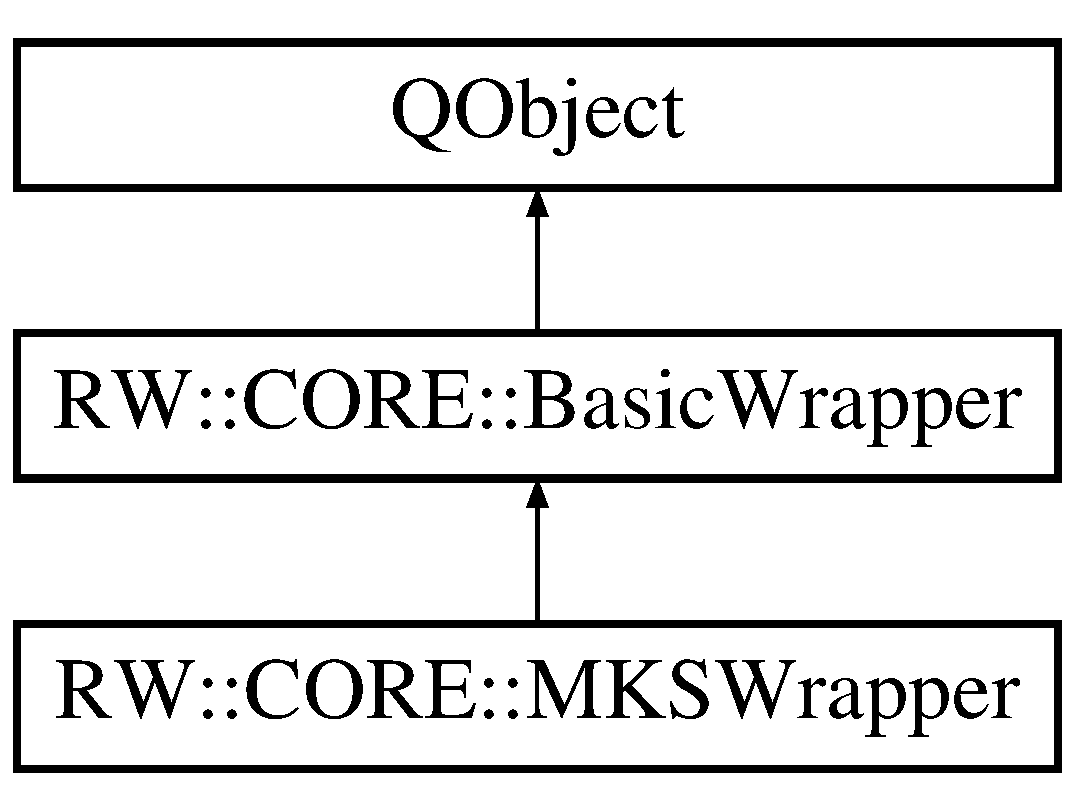
\includegraphics[height=3.000000cm]{class_r_w_1_1_c_o_r_e_1_1_m_k_s_wrapper}
\end{center}
\end{figure}
\subsection*{Public Slots}
\begin{DoxyCompactItemize}
\item 
virtual void \hyperlink{class_r_w_1_1_c_o_r_e_1_1_m_k_s_wrapper_ad3fa59666812d348b35467c1aa8d02d6}{On\+Process\+Message} (Util\+::\+Message\+Receiver Type, Util\+::\+Functions Func, Q\+Byte\+Array Report)
\end{DoxyCompactItemize}
\subsection*{Public Member Functions}
\begin{DoxyCompactItemize}
\item 
\hyperlink{class_r_w_1_1_c_o_r_e_1_1_m_k_s_wrapper_a003d8db211e3b1f38613b6a886540efb}{M\+K\+S\+Wrapper} (Q\+Object $\ast$Parent=nullptr)
\item 
\hyperlink{class_r_w_1_1_c_o_r_e_1_1_m_k_s_wrapper_a3e40623126c1ac27fa48d0065ed1afab}{$\sim$\+M\+K\+S\+Wrapper} ()
\end{DoxyCompactItemize}
\subsection*{Private Member Functions}
\begin{DoxyCompactItemize}
\item 
void \hyperlink{class_r_w_1_1_c_o_r_e_1_1_m_k_s_wrapper_ae6f651398e83b56aca4b9f0da3e417de}{Start\+M\+KS} (Q\+String M\+K\+S\+Location, Q\+String Username, Q\+String Password, Q\+String Server=\char`\"{}ims-\/id\char`\"{}, quint16 Port=7001, Q\+String Proxy=\char`\"{}M\+KS-\/P\+R\+O\+XY\char`\"{}, quint16 Proxy\+Port=7023)
\item 
void \hyperlink{class_r_w_1_1_c_o_r_e_1_1_m_k_s_wrapper_a75d87604a9244ce6e3a41934dd60b28f}{Create\+Sand\+Box} (Q\+String Mks\+Url, Q\+String Destination)
\item 
void \hyperlink{class_r_w_1_1_c_o_r_e_1_1_m_k_s_wrapper_a1f4bcd6096a326fc1329f1d63e207ec3}{Drop\+Sand\+Box} ()
\item 
Q\+String \hyperlink{class_r_w_1_1_c_o_r_e_1_1_m_k_s_wrapper_af8af87ae9a71d99e47e90b880091a604}{Get\+M\+K\+S\+Link} (Q\+String Mks\+Link)
\end{DoxyCompactItemize}
\subsection*{Private Attributes}
\begin{DoxyCompactItemize}
\item 
Q\+String \hyperlink{class_r_w_1_1_c_o_r_e_1_1_m_k_s_wrapper_a29a3be9d63ce87c3c4eaa17ac058c358}{m\+\_\+\+M\+K\+S\+Location}
\item 
Q\+String \hyperlink{class_r_w_1_1_c_o_r_e_1_1_m_k_s_wrapper_ae692d4f39fa2ff103a409afd2400bd50}{m\+\_\+\+Server}
\item 
Q\+String \hyperlink{class_r_w_1_1_c_o_r_e_1_1_m_k_s_wrapper_a61772018c0b8e4a38b4576dd93c00949}{m\+\_\+\+Proxy\+Server}
\item 
quint16 \hyperlink{class_r_w_1_1_c_o_r_e_1_1_m_k_s_wrapper_a9f64eb7e96f76b3af19530374954de92}{m\+\_\+\+Proxy\+Port}
\item 
quint16 \hyperlink{class_r_w_1_1_c_o_r_e_1_1_m_k_s_wrapper_a926dfddf01bc5e1815d4172b10733470}{m\+\_\+\+Port}
\item 
Q\+String \hyperlink{class_r_w_1_1_c_o_r_e_1_1_m_k_s_wrapper_a04dc61f3e323398af1c199e2ff044462}{m\+\_\+\+Destination}
\end{DoxyCompactItemize}
\subsection*{Additional Inherited Members}


\subsection{Detailed Description}


Definition at line 10 of file M\+K\+S\+Wrapper.\+h.



\subsection{Constructor \& Destructor Documentation}
\hypertarget{class_r_w_1_1_c_o_r_e_1_1_m_k_s_wrapper_a003d8db211e3b1f38613b6a886540efb}{}\label{class_r_w_1_1_c_o_r_e_1_1_m_k_s_wrapper_a003d8db211e3b1f38613b6a886540efb} 
\index{R\+W\+::\+C\+O\+R\+E\+::\+M\+K\+S\+Wrapper@{R\+W\+::\+C\+O\+R\+E\+::\+M\+K\+S\+Wrapper}!M\+K\+S\+Wrapper@{M\+K\+S\+Wrapper}}
\index{M\+K\+S\+Wrapper@{M\+K\+S\+Wrapper}!R\+W\+::\+C\+O\+R\+E\+::\+M\+K\+S\+Wrapper@{R\+W\+::\+C\+O\+R\+E\+::\+M\+K\+S\+Wrapper}}
\subsubsection{\texorpdfstring{M\+K\+S\+Wrapper()}{MKSWrapper()}}
{\footnotesize\ttfamily R\+W\+::\+C\+O\+R\+E\+::\+M\+K\+S\+Wrapper\+::\+M\+K\+S\+Wrapper (\begin{DoxyParamCaption}\item[{Q\+Object $\ast$}]{Parent = {\ttfamily nullptr} }\end{DoxyParamCaption})}



Definition at line 74 of file M\+K\+S\+Wrapper.\+cpp.

\hypertarget{class_r_w_1_1_c_o_r_e_1_1_m_k_s_wrapper_a3e40623126c1ac27fa48d0065ed1afab}{}\label{class_r_w_1_1_c_o_r_e_1_1_m_k_s_wrapper_a3e40623126c1ac27fa48d0065ed1afab} 
\index{R\+W\+::\+C\+O\+R\+E\+::\+M\+K\+S\+Wrapper@{R\+W\+::\+C\+O\+R\+E\+::\+M\+K\+S\+Wrapper}!````~M\+K\+S\+Wrapper@{$\sim$\+M\+K\+S\+Wrapper}}
\index{````~M\+K\+S\+Wrapper@{$\sim$\+M\+K\+S\+Wrapper}!R\+W\+::\+C\+O\+R\+E\+::\+M\+K\+S\+Wrapper@{R\+W\+::\+C\+O\+R\+E\+::\+M\+K\+S\+Wrapper}}
\subsubsection{\texorpdfstring{$\sim$\+M\+K\+S\+Wrapper()}{~MKSWrapper()}}
{\footnotesize\ttfamily R\+W\+::\+C\+O\+R\+E\+::\+M\+K\+S\+Wrapper\+::$\sim$\+M\+K\+S\+Wrapper (\begin{DoxyParamCaption}{ }\end{DoxyParamCaption})}



Definition at line 81 of file M\+K\+S\+Wrapper.\+cpp.



\subsection{Member Function Documentation}
\hypertarget{class_r_w_1_1_c_o_r_e_1_1_m_k_s_wrapper_a75d87604a9244ce6e3a41934dd60b28f}{}\label{class_r_w_1_1_c_o_r_e_1_1_m_k_s_wrapper_a75d87604a9244ce6e3a41934dd60b28f} 
\index{R\+W\+::\+C\+O\+R\+E\+::\+M\+K\+S\+Wrapper@{R\+W\+::\+C\+O\+R\+E\+::\+M\+K\+S\+Wrapper}!Create\+Sand\+Box@{Create\+Sand\+Box}}
\index{Create\+Sand\+Box@{Create\+Sand\+Box}!R\+W\+::\+C\+O\+R\+E\+::\+M\+K\+S\+Wrapper@{R\+W\+::\+C\+O\+R\+E\+::\+M\+K\+S\+Wrapper}}
\subsubsection{\texorpdfstring{Create\+Sand\+Box()}{CreateSandBox()}}
{\footnotesize\ttfamily void R\+W\+::\+C\+O\+R\+E\+::\+M\+K\+S\+Wrapper\+::\+Create\+Sand\+Box (\begin{DoxyParamCaption}\item[{Q\+String}]{Mks\+Url,  }\item[{Q\+String}]{Destination }\end{DoxyParamCaption})\hspace{0.3cm}{\ttfamily [private]}}



Definition at line 231 of file M\+K\+S\+Wrapper.\+cpp.

\hypertarget{class_r_w_1_1_c_o_r_e_1_1_m_k_s_wrapper_a1f4bcd6096a326fc1329f1d63e207ec3}{}\label{class_r_w_1_1_c_o_r_e_1_1_m_k_s_wrapper_a1f4bcd6096a326fc1329f1d63e207ec3} 
\index{R\+W\+::\+C\+O\+R\+E\+::\+M\+K\+S\+Wrapper@{R\+W\+::\+C\+O\+R\+E\+::\+M\+K\+S\+Wrapper}!Drop\+Sand\+Box@{Drop\+Sand\+Box}}
\index{Drop\+Sand\+Box@{Drop\+Sand\+Box}!R\+W\+::\+C\+O\+R\+E\+::\+M\+K\+S\+Wrapper@{R\+W\+::\+C\+O\+R\+E\+::\+M\+K\+S\+Wrapper}}
\subsubsection{\texorpdfstring{Drop\+Sand\+Box()}{DropSandBox()}}
{\footnotesize\ttfamily void R\+W\+::\+C\+O\+R\+E\+::\+M\+K\+S\+Wrapper\+::\+Drop\+Sand\+Box (\begin{DoxyParamCaption}{ }\end{DoxyParamCaption})\hspace{0.3cm}{\ttfamily [private]}}



Definition at line 277 of file M\+K\+S\+Wrapper.\+cpp.

\hypertarget{class_r_w_1_1_c_o_r_e_1_1_m_k_s_wrapper_af8af87ae9a71d99e47e90b880091a604}{}\label{class_r_w_1_1_c_o_r_e_1_1_m_k_s_wrapper_af8af87ae9a71d99e47e90b880091a604} 
\index{R\+W\+::\+C\+O\+R\+E\+::\+M\+K\+S\+Wrapper@{R\+W\+::\+C\+O\+R\+E\+::\+M\+K\+S\+Wrapper}!Get\+M\+K\+S\+Link@{Get\+M\+K\+S\+Link}}
\index{Get\+M\+K\+S\+Link@{Get\+M\+K\+S\+Link}!R\+W\+::\+C\+O\+R\+E\+::\+M\+K\+S\+Wrapper@{R\+W\+::\+C\+O\+R\+E\+::\+M\+K\+S\+Wrapper}}
\subsubsection{\texorpdfstring{Get\+M\+K\+S\+Link()}{GetMKSLink()}}
{\footnotesize\ttfamily Q\+String R\+W\+::\+C\+O\+R\+E\+::\+M\+K\+S\+Wrapper\+::\+Get\+M\+K\+S\+Link (\begin{DoxyParamCaption}\item[{Q\+String}]{Mks\+Link }\end{DoxyParamCaption})\hspace{0.3cm}{\ttfamily [private]}}



Definition at line 293 of file M\+K\+S\+Wrapper.\+cpp.

\hypertarget{class_r_w_1_1_c_o_r_e_1_1_m_k_s_wrapper_ad3fa59666812d348b35467c1aa8d02d6}{}\label{class_r_w_1_1_c_o_r_e_1_1_m_k_s_wrapper_ad3fa59666812d348b35467c1aa8d02d6} 
\index{R\+W\+::\+C\+O\+R\+E\+::\+M\+K\+S\+Wrapper@{R\+W\+::\+C\+O\+R\+E\+::\+M\+K\+S\+Wrapper}!On\+Process\+Message@{On\+Process\+Message}}
\index{On\+Process\+Message@{On\+Process\+Message}!R\+W\+::\+C\+O\+R\+E\+::\+M\+K\+S\+Wrapper@{R\+W\+::\+C\+O\+R\+E\+::\+M\+K\+S\+Wrapper}}
\subsubsection{\texorpdfstring{On\+Process\+Message}{OnProcessMessage}}
{\footnotesize\ttfamily void R\+W\+::\+C\+O\+R\+E\+::\+M\+K\+S\+Wrapper\+::\+On\+Process\+Message (\begin{DoxyParamCaption}\item[{Util\+::\+Message\+Receiver}]{Type,  }\item[{Util\+::\+Functions}]{Func,  }\item[{Q\+Byte\+Array}]{Report }\end{DoxyParamCaption})\hspace{0.3cm}{\ttfamily [virtual]}, {\ttfamily [slot]}}



Definition at line 85 of file M\+K\+S\+Wrapper.\+cpp.

\hypertarget{class_r_w_1_1_c_o_r_e_1_1_m_k_s_wrapper_ae6f651398e83b56aca4b9f0da3e417de}{}\label{class_r_w_1_1_c_o_r_e_1_1_m_k_s_wrapper_ae6f651398e83b56aca4b9f0da3e417de} 
\index{R\+W\+::\+C\+O\+R\+E\+::\+M\+K\+S\+Wrapper@{R\+W\+::\+C\+O\+R\+E\+::\+M\+K\+S\+Wrapper}!Start\+M\+KS@{Start\+M\+KS}}
\index{Start\+M\+KS@{Start\+M\+KS}!R\+W\+::\+C\+O\+R\+E\+::\+M\+K\+S\+Wrapper@{R\+W\+::\+C\+O\+R\+E\+::\+M\+K\+S\+Wrapper}}
\subsubsection{\texorpdfstring{Start\+M\+K\+S()}{StartMKS()}}
{\footnotesize\ttfamily void R\+W\+::\+C\+O\+R\+E\+::\+M\+K\+S\+Wrapper\+::\+Start\+M\+KS (\begin{DoxyParamCaption}\item[{Q\+String}]{M\+K\+S\+Location,  }\item[{Q\+String}]{Username,  }\item[{Q\+String}]{Password,  }\item[{Q\+String}]{Server = {\ttfamily \char`\"{}ims-\/id\char`\"{}},  }\item[{quint16}]{Port = {\ttfamily 7001},  }\item[{Q\+String}]{Proxy = {\ttfamily \char`\"{}MKS-\/PROXY\char`\"{}},  }\item[{quint16}]{Proxy\+Port = {\ttfamily 7023} }\end{DoxyParamCaption})\hspace{0.3cm}{\ttfamily [private]}}



Definition at line 131 of file M\+K\+S\+Wrapper.\+cpp.



\subsection{Member Data Documentation}
\hypertarget{class_r_w_1_1_c_o_r_e_1_1_m_k_s_wrapper_a04dc61f3e323398af1c199e2ff044462}{}\label{class_r_w_1_1_c_o_r_e_1_1_m_k_s_wrapper_a04dc61f3e323398af1c199e2ff044462} 
\index{R\+W\+::\+C\+O\+R\+E\+::\+M\+K\+S\+Wrapper@{R\+W\+::\+C\+O\+R\+E\+::\+M\+K\+S\+Wrapper}!m\+\_\+\+Destination@{m\+\_\+\+Destination}}
\index{m\+\_\+\+Destination@{m\+\_\+\+Destination}!R\+W\+::\+C\+O\+R\+E\+::\+M\+K\+S\+Wrapper@{R\+W\+::\+C\+O\+R\+E\+::\+M\+K\+S\+Wrapper}}
\subsubsection{\texorpdfstring{m\+\_\+\+Destination}{m\_Destination}}
{\footnotesize\ttfamily Q\+String R\+W\+::\+C\+O\+R\+E\+::\+M\+K\+S\+Wrapper\+::m\+\_\+\+Destination\hspace{0.3cm}{\ttfamily [private]}}



Definition at line 20 of file M\+K\+S\+Wrapper.\+h.

\hypertarget{class_r_w_1_1_c_o_r_e_1_1_m_k_s_wrapper_a29a3be9d63ce87c3c4eaa17ac058c358}{}\label{class_r_w_1_1_c_o_r_e_1_1_m_k_s_wrapper_a29a3be9d63ce87c3c4eaa17ac058c358} 
\index{R\+W\+::\+C\+O\+R\+E\+::\+M\+K\+S\+Wrapper@{R\+W\+::\+C\+O\+R\+E\+::\+M\+K\+S\+Wrapper}!m\+\_\+\+M\+K\+S\+Location@{m\+\_\+\+M\+K\+S\+Location}}
\index{m\+\_\+\+M\+K\+S\+Location@{m\+\_\+\+M\+K\+S\+Location}!R\+W\+::\+C\+O\+R\+E\+::\+M\+K\+S\+Wrapper@{R\+W\+::\+C\+O\+R\+E\+::\+M\+K\+S\+Wrapper}}
\subsubsection{\texorpdfstring{m\+\_\+\+M\+K\+S\+Location}{m\_MKSLocation}}
{\footnotesize\ttfamily Q\+String R\+W\+::\+C\+O\+R\+E\+::\+M\+K\+S\+Wrapper\+::m\+\_\+\+M\+K\+S\+Location\hspace{0.3cm}{\ttfamily [private]}}



Definition at line 15 of file M\+K\+S\+Wrapper.\+h.

\hypertarget{class_r_w_1_1_c_o_r_e_1_1_m_k_s_wrapper_a926dfddf01bc5e1815d4172b10733470}{}\label{class_r_w_1_1_c_o_r_e_1_1_m_k_s_wrapper_a926dfddf01bc5e1815d4172b10733470} 
\index{R\+W\+::\+C\+O\+R\+E\+::\+M\+K\+S\+Wrapper@{R\+W\+::\+C\+O\+R\+E\+::\+M\+K\+S\+Wrapper}!m\+\_\+\+Port@{m\+\_\+\+Port}}
\index{m\+\_\+\+Port@{m\+\_\+\+Port}!R\+W\+::\+C\+O\+R\+E\+::\+M\+K\+S\+Wrapper@{R\+W\+::\+C\+O\+R\+E\+::\+M\+K\+S\+Wrapper}}
\subsubsection{\texorpdfstring{m\+\_\+\+Port}{m\_Port}}
{\footnotesize\ttfamily quint16 R\+W\+::\+C\+O\+R\+E\+::\+M\+K\+S\+Wrapper\+::m\+\_\+\+Port\hspace{0.3cm}{\ttfamily [private]}}



Definition at line 19 of file M\+K\+S\+Wrapper.\+h.

\hypertarget{class_r_w_1_1_c_o_r_e_1_1_m_k_s_wrapper_a9f64eb7e96f76b3af19530374954de92}{}\label{class_r_w_1_1_c_o_r_e_1_1_m_k_s_wrapper_a9f64eb7e96f76b3af19530374954de92} 
\index{R\+W\+::\+C\+O\+R\+E\+::\+M\+K\+S\+Wrapper@{R\+W\+::\+C\+O\+R\+E\+::\+M\+K\+S\+Wrapper}!m\+\_\+\+Proxy\+Port@{m\+\_\+\+Proxy\+Port}}
\index{m\+\_\+\+Proxy\+Port@{m\+\_\+\+Proxy\+Port}!R\+W\+::\+C\+O\+R\+E\+::\+M\+K\+S\+Wrapper@{R\+W\+::\+C\+O\+R\+E\+::\+M\+K\+S\+Wrapper}}
\subsubsection{\texorpdfstring{m\+\_\+\+Proxy\+Port}{m\_ProxyPort}}
{\footnotesize\ttfamily quint16 R\+W\+::\+C\+O\+R\+E\+::\+M\+K\+S\+Wrapper\+::m\+\_\+\+Proxy\+Port\hspace{0.3cm}{\ttfamily [private]}}



Definition at line 18 of file M\+K\+S\+Wrapper.\+h.

\hypertarget{class_r_w_1_1_c_o_r_e_1_1_m_k_s_wrapper_a61772018c0b8e4a38b4576dd93c00949}{}\label{class_r_w_1_1_c_o_r_e_1_1_m_k_s_wrapper_a61772018c0b8e4a38b4576dd93c00949} 
\index{R\+W\+::\+C\+O\+R\+E\+::\+M\+K\+S\+Wrapper@{R\+W\+::\+C\+O\+R\+E\+::\+M\+K\+S\+Wrapper}!m\+\_\+\+Proxy\+Server@{m\+\_\+\+Proxy\+Server}}
\index{m\+\_\+\+Proxy\+Server@{m\+\_\+\+Proxy\+Server}!R\+W\+::\+C\+O\+R\+E\+::\+M\+K\+S\+Wrapper@{R\+W\+::\+C\+O\+R\+E\+::\+M\+K\+S\+Wrapper}}
\subsubsection{\texorpdfstring{m\+\_\+\+Proxy\+Server}{m\_ProxyServer}}
{\footnotesize\ttfamily Q\+String R\+W\+::\+C\+O\+R\+E\+::\+M\+K\+S\+Wrapper\+::m\+\_\+\+Proxy\+Server\hspace{0.3cm}{\ttfamily [private]}}



Definition at line 17 of file M\+K\+S\+Wrapper.\+h.

\hypertarget{class_r_w_1_1_c_o_r_e_1_1_m_k_s_wrapper_ae692d4f39fa2ff103a409afd2400bd50}{}\label{class_r_w_1_1_c_o_r_e_1_1_m_k_s_wrapper_ae692d4f39fa2ff103a409afd2400bd50} 
\index{R\+W\+::\+C\+O\+R\+E\+::\+M\+K\+S\+Wrapper@{R\+W\+::\+C\+O\+R\+E\+::\+M\+K\+S\+Wrapper}!m\+\_\+\+Server@{m\+\_\+\+Server}}
\index{m\+\_\+\+Server@{m\+\_\+\+Server}!R\+W\+::\+C\+O\+R\+E\+::\+M\+K\+S\+Wrapper@{R\+W\+::\+C\+O\+R\+E\+::\+M\+K\+S\+Wrapper}}
\subsubsection{\texorpdfstring{m\+\_\+\+Server}{m\_Server}}
{\footnotesize\ttfamily Q\+String R\+W\+::\+C\+O\+R\+E\+::\+M\+K\+S\+Wrapper\+::m\+\_\+\+Server\hspace{0.3cm}{\ttfamily [private]}}



Definition at line 16 of file M\+K\+S\+Wrapper.\+h.



The documentation for this class was generated from the following files\+:\begin{DoxyCompactItemize}
\item 
C\+:/\+Projekte/\+Remote\+Repros/\+Remote\+Hidden\+Helper/\+Remote\+Hidden\+Helper/\hyperlink{_m_k_s_wrapper_8h}{M\+K\+S\+Wrapper.\+h}\item 
C\+:/\+Projekte/\+Remote\+Repros/\+Remote\+Hidden\+Helper/\+Remote\+Hidden\+Helper/\hyperlink{_m_k_s_wrapper_8cpp}{M\+K\+S\+Wrapper.\+cpp}\end{DoxyCompactItemize}

\hypertarget{class_r_w_1_1_c_o_r_e_1_1_portal_info}{}\section{RW\+:\+:C\+O\+RE\+:\+:Portal\+Info Class Reference}
\label{class_r_w_1_1_c_o_r_e_1_1_portal_info}\index{R\+W\+::\+C\+O\+R\+E\+::\+Portal\+Info@{R\+W\+::\+C\+O\+R\+E\+::\+Portal\+Info}}


{\ttfamily \#include $<$Portal\+Info.\+h$>$}

Inheritance diagram for RW\+:\+:C\+O\+RE\+:\+:Portal\+Info\+:\begin{figure}[H]
\begin{center}
\leavevmode
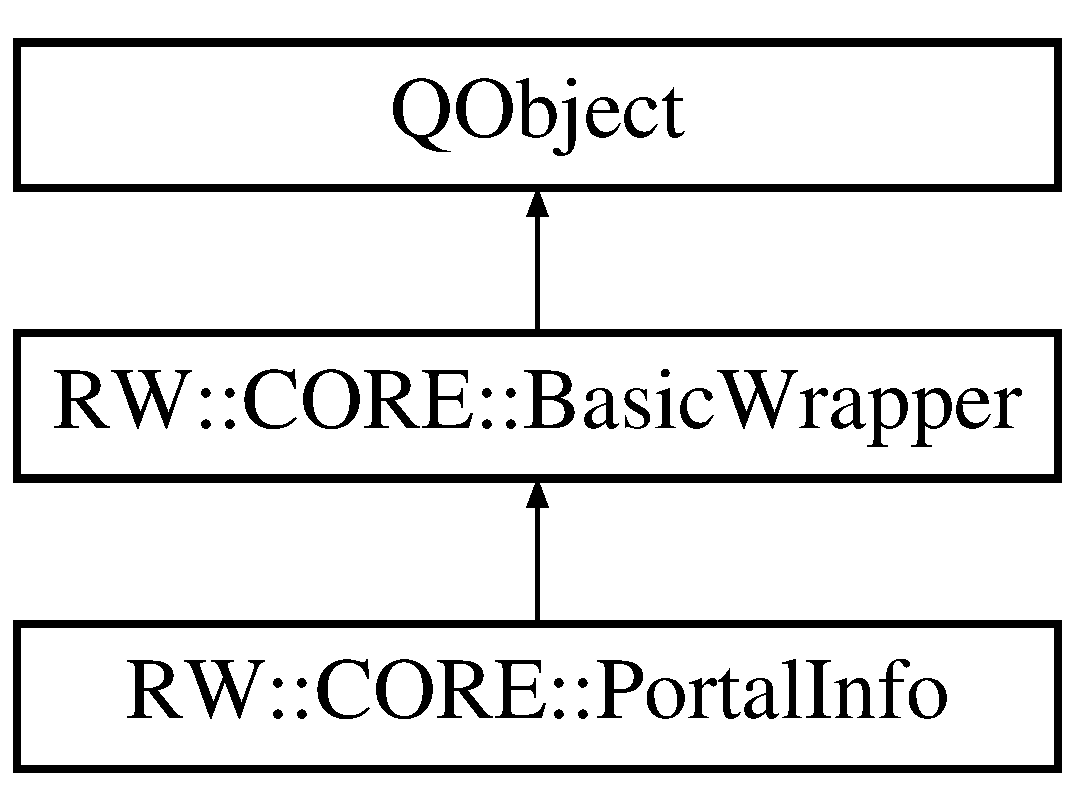
\includegraphics[height=3.000000cm]{class_r_w_1_1_c_o_r_e_1_1_portal_info}
\end{center}
\end{figure}
\subsection*{Public Slots}
\begin{DoxyCompactItemize}
\item 
virtual void \hyperlink{class_r_w_1_1_c_o_r_e_1_1_portal_info_aa564efcfe704d21d9504e57ea76f59b9}{On\+Process\+Message} (Util\+::\+Message\+Receiver Type, Util\+::\+Functions Func, Q\+Byte\+Array Report)
\end{DoxyCompactItemize}
\subsection*{Public Member Functions}
\begin{DoxyCompactItemize}
\item 
\hyperlink{class_r_w_1_1_c_o_r_e_1_1_portal_info_a9f2c368244ee835c72aae72c40b4dc7f}{Portal\+Info} (Q\+Object $\ast$Parent=nullptr)
\item 
\hyperlink{class_r_w_1_1_c_o_r_e_1_1_portal_info_a9bc69018c7e68b82bf4406cd62310e5c}{$\sim$\+Portal\+Info} ()
\end{DoxyCompactItemize}
\subsection*{Private Slots}
\begin{DoxyCompactItemize}
\item 
Util\+::\+Error\+ID \hyperlink{class_r_w_1_1_c_o_r_e_1_1_portal_info_af67bdf39beece4b3fb27c9f1a14ecbd7}{Fill\+Project\+Combobox} ()
\item 
Util\+::\+Error\+ID \hyperlink{class_r_w_1_1_c_o_r_e_1_1_portal_info_a3f22e04d628d3907cff56e3617dda192}{Fill\+Sample\+Phase\+Combobox} (const Q\+String \&Selected\+Project)
\item 
Util\+::\+Error\+ID \hyperlink{class_r_w_1_1_c_o_r_e_1_1_portal_info_ad9f44cdba6c3c3aa901e45d8a503c13f}{Fill\+Release\+Combobox} (const Q\+String \&Selected\+Sample\+Phase)
\end{DoxyCompactItemize}
\subsection*{Private Member Functions}
\begin{DoxyCompactItemize}
\item 
void \hyperlink{class_r_w_1_1_c_o_r_e_1_1_portal_info_aeb0d50467997e59088be9f5b952916f7}{Highligh\+Check\+Boxes} ()
\item 
void \hyperlink{class_r_w_1_1_c_o_r_e_1_1_portal_info_a9f104d772b07f236cb0f8e0c0c46461c}{Highlight\+Combo\+Boxes} (Q\+Label $\ast$Highlight)
\item 
void \hyperlink{class_r_w_1_1_c_o_r_e_1_1_portal_info_a76776e5e5e56da7ff882748881a89b65}{Normalize\+Check\+Boxes} ()
\item 
void \hyperlink{class_r_w_1_1_c_o_r_e_1_1_portal_info_a6d1f3e606e52aa278cadeb7ae8846887}{Normalize\+Combo\+Boxes} ()
\item 
void \hyperlink{class_r_w_1_1_c_o_r_e_1_1_portal_info_a8b87b8289b8d980540c3121e2e82b405}{Show\+Dialog} ()
\item 
void \hyperlink{class_r_w_1_1_c_o_r_e_1_1_portal_info_a4ecfa598aff3ba559d65dcb8a78f3715}{Close\+Dialog} ()
\item 
void \hyperlink{class_r_w_1_1_c_o_r_e_1_1_portal_info_af72c1360fe61113175d39791b18312e1}{Flash} ()
\end{DoxyCompactItemize}
\subsection*{Private Attributes}
\begin{DoxyCompactItemize}
\item 
Q\+Main\+Window $\ast$ \hyperlink{class_r_w_1_1_c_o_r_e_1_1_portal_info_ab377e834cdc7264c3d7f0d7c35c2bc6f}{m\+\_\+\+Dialog}
\item 
\hyperlink{class_ui_1_1_remote_hidden_helper_class}{Ui\+::\+Remote\+Hidden\+Helper\+Class} $\ast$ \hyperlink{class_r_w_1_1_c_o_r_e_1_1_portal_info_a8c82ce1d24c210b2e24f6844be8172ff}{m\+\_\+ui}
\item 
\hyperlink{class_r_w_1_1_c_o_r_e_1_1_flash_informations}{Flash\+Informations} $\ast$ \hyperlink{class_r_w_1_1_c_o_r_e_1_1_portal_info_a2cf39162f662b4cc27ee32edbe360907}{m\+\_\+\+Flash\+Informationen}
\end{DoxyCompactItemize}
\subsection*{Additional Inherited Members}


\subsection{Detailed Description}


Definition at line 24 of file Portal\+Info.\+h.



\subsection{Constructor \& Destructor Documentation}
\hypertarget{class_r_w_1_1_c_o_r_e_1_1_portal_info_a9f2c368244ee835c72aae72c40b4dc7f}{}\label{class_r_w_1_1_c_o_r_e_1_1_portal_info_a9f2c368244ee835c72aae72c40b4dc7f} 
\index{R\+W\+::\+C\+O\+R\+E\+::\+Portal\+Info@{R\+W\+::\+C\+O\+R\+E\+::\+Portal\+Info}!Portal\+Info@{Portal\+Info}}
\index{Portal\+Info@{Portal\+Info}!R\+W\+::\+C\+O\+R\+E\+::\+Portal\+Info@{R\+W\+::\+C\+O\+R\+E\+::\+Portal\+Info}}
\subsubsection{\texorpdfstring{Portal\+Info()}{PortalInfo()}}
{\footnotesize\ttfamily R\+W\+::\+C\+O\+R\+E\+::\+Portal\+Info\+::\+Portal\+Info (\begin{DoxyParamCaption}\item[{Q\+Object $\ast$}]{Parent = {\ttfamily nullptr} }\end{DoxyParamCaption})}



Definition at line 22 of file Portal\+Info.\+cpp.

\hypertarget{class_r_w_1_1_c_o_r_e_1_1_portal_info_a9bc69018c7e68b82bf4406cd62310e5c}{}\label{class_r_w_1_1_c_o_r_e_1_1_portal_info_a9bc69018c7e68b82bf4406cd62310e5c} 
\index{R\+W\+::\+C\+O\+R\+E\+::\+Portal\+Info@{R\+W\+::\+C\+O\+R\+E\+::\+Portal\+Info}!````~Portal\+Info@{$\sim$\+Portal\+Info}}
\index{````~Portal\+Info@{$\sim$\+Portal\+Info}!R\+W\+::\+C\+O\+R\+E\+::\+Portal\+Info@{R\+W\+::\+C\+O\+R\+E\+::\+Portal\+Info}}
\subsubsection{\texorpdfstring{$\sim$\+Portal\+Info()}{~PortalInfo()}}
{\footnotesize\ttfamily R\+W\+::\+C\+O\+R\+E\+::\+Portal\+Info\+::$\sim$\+Portal\+Info (\begin{DoxyParamCaption}{ }\end{DoxyParamCaption})}



Definition at line 30 of file Portal\+Info.\+cpp.



\subsection{Member Function Documentation}
\hypertarget{class_r_w_1_1_c_o_r_e_1_1_portal_info_a4ecfa598aff3ba559d65dcb8a78f3715}{}\label{class_r_w_1_1_c_o_r_e_1_1_portal_info_a4ecfa598aff3ba559d65dcb8a78f3715} 
\index{R\+W\+::\+C\+O\+R\+E\+::\+Portal\+Info@{R\+W\+::\+C\+O\+R\+E\+::\+Portal\+Info}!Close\+Dialog@{Close\+Dialog}}
\index{Close\+Dialog@{Close\+Dialog}!R\+W\+::\+C\+O\+R\+E\+::\+Portal\+Info@{R\+W\+::\+C\+O\+R\+E\+::\+Portal\+Info}}
\subsubsection{\texorpdfstring{Close\+Dialog()}{CloseDialog()}}
{\footnotesize\ttfamily void R\+W\+::\+C\+O\+R\+E\+::\+Portal\+Info\+::\+Close\+Dialog (\begin{DoxyParamCaption}{ }\end{DoxyParamCaption})\hspace{0.3cm}{\ttfamily [private]}}



Definition at line 92 of file Portal\+Info.\+cpp.

\hypertarget{class_r_w_1_1_c_o_r_e_1_1_portal_info_af67bdf39beece4b3fb27c9f1a14ecbd7}{}\label{class_r_w_1_1_c_o_r_e_1_1_portal_info_af67bdf39beece4b3fb27c9f1a14ecbd7} 
\index{R\+W\+::\+C\+O\+R\+E\+::\+Portal\+Info@{R\+W\+::\+C\+O\+R\+E\+::\+Portal\+Info}!Fill\+Project\+Combobox@{Fill\+Project\+Combobox}}
\index{Fill\+Project\+Combobox@{Fill\+Project\+Combobox}!R\+W\+::\+C\+O\+R\+E\+::\+Portal\+Info@{R\+W\+::\+C\+O\+R\+E\+::\+Portal\+Info}}
\subsubsection{\texorpdfstring{Fill\+Project\+Combobox}{FillProjectCombobox}}
{\footnotesize\ttfamily Util\+::\+Error\+ID R\+W\+::\+C\+O\+R\+E\+::\+Portal\+Info\+::\+Fill\+Project\+Combobox (\begin{DoxyParamCaption}{ }\end{DoxyParamCaption})\hspace{0.3cm}{\ttfamily [private]}, {\ttfamily [slot]}}



Definition at line 99 of file Portal\+Info.\+cpp.

\hypertarget{class_r_w_1_1_c_o_r_e_1_1_portal_info_ad9f44cdba6c3c3aa901e45d8a503c13f}{}\label{class_r_w_1_1_c_o_r_e_1_1_portal_info_ad9f44cdba6c3c3aa901e45d8a503c13f} 
\index{R\+W\+::\+C\+O\+R\+E\+::\+Portal\+Info@{R\+W\+::\+C\+O\+R\+E\+::\+Portal\+Info}!Fill\+Release\+Combobox@{Fill\+Release\+Combobox}}
\index{Fill\+Release\+Combobox@{Fill\+Release\+Combobox}!R\+W\+::\+C\+O\+R\+E\+::\+Portal\+Info@{R\+W\+::\+C\+O\+R\+E\+::\+Portal\+Info}}
\subsubsection{\texorpdfstring{Fill\+Release\+Combobox}{FillReleaseCombobox}}
{\footnotesize\ttfamily Util\+::\+Error\+ID R\+W\+::\+C\+O\+R\+E\+::\+Portal\+Info\+::\+Fill\+Release\+Combobox (\begin{DoxyParamCaption}\item[{const Q\+String \&}]{Selected\+Sample\+Phase }\end{DoxyParamCaption})\hspace{0.3cm}{\ttfamily [private]}, {\ttfamily [slot]}}



Definition at line 135 of file Portal\+Info.\+cpp.

\hypertarget{class_r_w_1_1_c_o_r_e_1_1_portal_info_a3f22e04d628d3907cff56e3617dda192}{}\label{class_r_w_1_1_c_o_r_e_1_1_portal_info_a3f22e04d628d3907cff56e3617dda192} 
\index{R\+W\+::\+C\+O\+R\+E\+::\+Portal\+Info@{R\+W\+::\+C\+O\+R\+E\+::\+Portal\+Info}!Fill\+Sample\+Phase\+Combobox@{Fill\+Sample\+Phase\+Combobox}}
\index{Fill\+Sample\+Phase\+Combobox@{Fill\+Sample\+Phase\+Combobox}!R\+W\+::\+C\+O\+R\+E\+::\+Portal\+Info@{R\+W\+::\+C\+O\+R\+E\+::\+Portal\+Info}}
\subsubsection{\texorpdfstring{Fill\+Sample\+Phase\+Combobox}{FillSamplePhaseCombobox}}
{\footnotesize\ttfamily Util\+::\+Error\+ID R\+W\+::\+C\+O\+R\+E\+::\+Portal\+Info\+::\+Fill\+Sample\+Phase\+Combobox (\begin{DoxyParamCaption}\item[{const Q\+String \&}]{Selected\+Project }\end{DoxyParamCaption})\hspace{0.3cm}{\ttfamily [private]}, {\ttfamily [slot]}}



Definition at line 117 of file Portal\+Info.\+cpp.

\hypertarget{class_r_w_1_1_c_o_r_e_1_1_portal_info_af72c1360fe61113175d39791b18312e1}{}\label{class_r_w_1_1_c_o_r_e_1_1_portal_info_af72c1360fe61113175d39791b18312e1} 
\index{R\+W\+::\+C\+O\+R\+E\+::\+Portal\+Info@{R\+W\+::\+C\+O\+R\+E\+::\+Portal\+Info}!Flash@{Flash}}
\index{Flash@{Flash}!R\+W\+::\+C\+O\+R\+E\+::\+Portal\+Info@{R\+W\+::\+C\+O\+R\+E\+::\+Portal\+Info}}
\subsubsection{\texorpdfstring{Flash()}{Flash()}}
{\footnotesize\ttfamily void R\+W\+::\+C\+O\+R\+E\+::\+Portal\+Info\+::\+Flash (\begin{DoxyParamCaption}{ }\end{DoxyParamCaption})\hspace{0.3cm}{\ttfamily [private]}}



Definition at line 149 of file Portal\+Info.\+cpp.

\hypertarget{class_r_w_1_1_c_o_r_e_1_1_portal_info_aeb0d50467997e59088be9f5b952916f7}{}\label{class_r_w_1_1_c_o_r_e_1_1_portal_info_aeb0d50467997e59088be9f5b952916f7} 
\index{R\+W\+::\+C\+O\+R\+E\+::\+Portal\+Info@{R\+W\+::\+C\+O\+R\+E\+::\+Portal\+Info}!Highligh\+Check\+Boxes@{Highligh\+Check\+Boxes}}
\index{Highligh\+Check\+Boxes@{Highligh\+Check\+Boxes}!R\+W\+::\+C\+O\+R\+E\+::\+Portal\+Info@{R\+W\+::\+C\+O\+R\+E\+::\+Portal\+Info}}
\subsubsection{\texorpdfstring{Highligh\+Check\+Boxes()}{HighlighCheckBoxes()}}
{\footnotesize\ttfamily void R\+W\+::\+C\+O\+R\+E\+::\+Portal\+Info\+::\+Highligh\+Check\+Boxes (\begin{DoxyParamCaption}{ }\end{DoxyParamCaption})\hspace{0.3cm}{\ttfamily [private]}}



Definition at line 255 of file Portal\+Info.\+cpp.

\hypertarget{class_r_w_1_1_c_o_r_e_1_1_portal_info_a9f104d772b07f236cb0f8e0c0c46461c}{}\label{class_r_w_1_1_c_o_r_e_1_1_portal_info_a9f104d772b07f236cb0f8e0c0c46461c} 
\index{R\+W\+::\+C\+O\+R\+E\+::\+Portal\+Info@{R\+W\+::\+C\+O\+R\+E\+::\+Portal\+Info}!Highlight\+Combo\+Boxes@{Highlight\+Combo\+Boxes}}
\index{Highlight\+Combo\+Boxes@{Highlight\+Combo\+Boxes}!R\+W\+::\+C\+O\+R\+E\+::\+Portal\+Info@{R\+W\+::\+C\+O\+R\+E\+::\+Portal\+Info}}
\subsubsection{\texorpdfstring{Highlight\+Combo\+Boxes()}{HighlightComboBoxes()}}
{\footnotesize\ttfamily void R\+W\+::\+C\+O\+R\+E\+::\+Portal\+Info\+::\+Highlight\+Combo\+Boxes (\begin{DoxyParamCaption}\item[{Q\+Label $\ast$}]{Highlight }\end{DoxyParamCaption})\hspace{0.3cm}{\ttfamily [private]}}



Definition at line 267 of file Portal\+Info.\+cpp.

\hypertarget{class_r_w_1_1_c_o_r_e_1_1_portal_info_a76776e5e5e56da7ff882748881a89b65}{}\label{class_r_w_1_1_c_o_r_e_1_1_portal_info_a76776e5e5e56da7ff882748881a89b65} 
\index{R\+W\+::\+C\+O\+R\+E\+::\+Portal\+Info@{R\+W\+::\+C\+O\+R\+E\+::\+Portal\+Info}!Normalize\+Check\+Boxes@{Normalize\+Check\+Boxes}}
\index{Normalize\+Check\+Boxes@{Normalize\+Check\+Boxes}!R\+W\+::\+C\+O\+R\+E\+::\+Portal\+Info@{R\+W\+::\+C\+O\+R\+E\+::\+Portal\+Info}}
\subsubsection{\texorpdfstring{Normalize\+Check\+Boxes()}{NormalizeCheckBoxes()}}
{\footnotesize\ttfamily void R\+W\+::\+C\+O\+R\+E\+::\+Portal\+Info\+::\+Normalize\+Check\+Boxes (\begin{DoxyParamCaption}{ }\end{DoxyParamCaption})\hspace{0.3cm}{\ttfamily [private]}}



Definition at line 272 of file Portal\+Info.\+cpp.

\hypertarget{class_r_w_1_1_c_o_r_e_1_1_portal_info_a6d1f3e606e52aa278cadeb7ae8846887}{}\label{class_r_w_1_1_c_o_r_e_1_1_portal_info_a6d1f3e606e52aa278cadeb7ae8846887} 
\index{R\+W\+::\+C\+O\+R\+E\+::\+Portal\+Info@{R\+W\+::\+C\+O\+R\+E\+::\+Portal\+Info}!Normalize\+Combo\+Boxes@{Normalize\+Combo\+Boxes}}
\index{Normalize\+Combo\+Boxes@{Normalize\+Combo\+Boxes}!R\+W\+::\+C\+O\+R\+E\+::\+Portal\+Info@{R\+W\+::\+C\+O\+R\+E\+::\+Portal\+Info}}
\subsubsection{\texorpdfstring{Normalize\+Combo\+Boxes()}{NormalizeComboBoxes()}}
{\footnotesize\ttfamily void R\+W\+::\+C\+O\+R\+E\+::\+Portal\+Info\+::\+Normalize\+Combo\+Boxes (\begin{DoxyParamCaption}{ }\end{DoxyParamCaption})\hspace{0.3cm}{\ttfamily [private]}}



Definition at line 284 of file Portal\+Info.\+cpp.

\hypertarget{class_r_w_1_1_c_o_r_e_1_1_portal_info_aa564efcfe704d21d9504e57ea76f59b9}{}\label{class_r_w_1_1_c_o_r_e_1_1_portal_info_aa564efcfe704d21d9504e57ea76f59b9} 
\index{R\+W\+::\+C\+O\+R\+E\+::\+Portal\+Info@{R\+W\+::\+C\+O\+R\+E\+::\+Portal\+Info}!On\+Process\+Message@{On\+Process\+Message}}
\index{On\+Process\+Message@{On\+Process\+Message}!R\+W\+::\+C\+O\+R\+E\+::\+Portal\+Info@{R\+W\+::\+C\+O\+R\+E\+::\+Portal\+Info}}
\subsubsection{\texorpdfstring{On\+Process\+Message}{OnProcessMessage}}
{\footnotesize\ttfamily void R\+W\+::\+C\+O\+R\+E\+::\+Portal\+Info\+::\+On\+Process\+Message (\begin{DoxyParamCaption}\item[{Util\+::\+Message\+Receiver}]{Type,  }\item[{Util\+::\+Functions}]{Func,  }\item[{Q\+Byte\+Array}]{Report }\end{DoxyParamCaption})\hspace{0.3cm}{\ttfamily [virtual]}, {\ttfamily [slot]}}



Definition at line 36 of file Portal\+Info.\+cpp.

\hypertarget{class_r_w_1_1_c_o_r_e_1_1_portal_info_a8b87b8289b8d980540c3121e2e82b405}{}\label{class_r_w_1_1_c_o_r_e_1_1_portal_info_a8b87b8289b8d980540c3121e2e82b405} 
\index{R\+W\+::\+C\+O\+R\+E\+::\+Portal\+Info@{R\+W\+::\+C\+O\+R\+E\+::\+Portal\+Info}!Show\+Dialog@{Show\+Dialog}}
\index{Show\+Dialog@{Show\+Dialog}!R\+W\+::\+C\+O\+R\+E\+::\+Portal\+Info@{R\+W\+::\+C\+O\+R\+E\+::\+Portal\+Info}}
\subsubsection{\texorpdfstring{Show\+Dialog()}{ShowDialog()}}
{\footnotesize\ttfamily void R\+W\+::\+C\+O\+R\+E\+::\+Portal\+Info\+::\+Show\+Dialog (\begin{DoxyParamCaption}{ }\end{DoxyParamCaption})\hspace{0.3cm}{\ttfamily [private]}}



Definition at line 70 of file Portal\+Info.\+cpp.



\subsection{Member Data Documentation}
\hypertarget{class_r_w_1_1_c_o_r_e_1_1_portal_info_ab377e834cdc7264c3d7f0d7c35c2bc6f}{}\label{class_r_w_1_1_c_o_r_e_1_1_portal_info_ab377e834cdc7264c3d7f0d7c35c2bc6f} 
\index{R\+W\+::\+C\+O\+R\+E\+::\+Portal\+Info@{R\+W\+::\+C\+O\+R\+E\+::\+Portal\+Info}!m\+\_\+\+Dialog@{m\+\_\+\+Dialog}}
\index{m\+\_\+\+Dialog@{m\+\_\+\+Dialog}!R\+W\+::\+C\+O\+R\+E\+::\+Portal\+Info@{R\+W\+::\+C\+O\+R\+E\+::\+Portal\+Info}}
\subsubsection{\texorpdfstring{m\+\_\+\+Dialog}{m\_Dialog}}
{\footnotesize\ttfamily Q\+Main\+Window$\ast$ R\+W\+::\+C\+O\+R\+E\+::\+Portal\+Info\+::m\+\_\+\+Dialog\hspace{0.3cm}{\ttfamily [private]}}



Definition at line 28 of file Portal\+Info.\+h.

\hypertarget{class_r_w_1_1_c_o_r_e_1_1_portal_info_a2cf39162f662b4cc27ee32edbe360907}{}\label{class_r_w_1_1_c_o_r_e_1_1_portal_info_a2cf39162f662b4cc27ee32edbe360907} 
\index{R\+W\+::\+C\+O\+R\+E\+::\+Portal\+Info@{R\+W\+::\+C\+O\+R\+E\+::\+Portal\+Info}!m\+\_\+\+Flash\+Informationen@{m\+\_\+\+Flash\+Informationen}}
\index{m\+\_\+\+Flash\+Informationen@{m\+\_\+\+Flash\+Informationen}!R\+W\+::\+C\+O\+R\+E\+::\+Portal\+Info@{R\+W\+::\+C\+O\+R\+E\+::\+Portal\+Info}}
\subsubsection{\texorpdfstring{m\+\_\+\+Flash\+Informationen}{m\_FlashInformationen}}
{\footnotesize\ttfamily \hyperlink{class_r_w_1_1_c_o_r_e_1_1_flash_informations}{Flash\+Informations}$\ast$ R\+W\+::\+C\+O\+R\+E\+::\+Portal\+Info\+::m\+\_\+\+Flash\+Informationen\hspace{0.3cm}{\ttfamily [private]}}



Definition at line 36 of file Portal\+Info.\+h.

\hypertarget{class_r_w_1_1_c_o_r_e_1_1_portal_info_a8c82ce1d24c210b2e24f6844be8172ff}{}\label{class_r_w_1_1_c_o_r_e_1_1_portal_info_a8c82ce1d24c210b2e24f6844be8172ff} 
\index{R\+W\+::\+C\+O\+R\+E\+::\+Portal\+Info@{R\+W\+::\+C\+O\+R\+E\+::\+Portal\+Info}!m\+\_\+ui@{m\+\_\+ui}}
\index{m\+\_\+ui@{m\+\_\+ui}!R\+W\+::\+C\+O\+R\+E\+::\+Portal\+Info@{R\+W\+::\+C\+O\+R\+E\+::\+Portal\+Info}}
\subsubsection{\texorpdfstring{m\+\_\+ui}{m\_ui}}
{\footnotesize\ttfamily \hyperlink{class_ui_1_1_remote_hidden_helper_class}{Ui\+::\+Remote\+Hidden\+Helper\+Class}$\ast$ R\+W\+::\+C\+O\+R\+E\+::\+Portal\+Info\+::m\+\_\+ui\hspace{0.3cm}{\ttfamily [private]}}



Definition at line 29 of file Portal\+Info.\+h.



The documentation for this class was generated from the following files\+:\begin{DoxyCompactItemize}
\item 
C\+:/\+Projekte/\+Remote\+Repros/\+Remote\+Hidden\+Helper/\+Remote\+Hidden\+Helper/\hyperlink{_portal_info_8h}{Portal\+Info.\+h}\item 
C\+:/\+Projekte/\+Remote\+Repros/\+Remote\+Hidden\+Helper/\+Remote\+Hidden\+Helper/\hyperlink{_portal_info_8cpp}{Portal\+Info.\+cpp}\end{DoxyCompactItemize}

\hypertarget{class_r_w_1_1_c_o_r_e_1_1_process_manager}{}\section{RW\+:\+:C\+O\+RE\+:\+:Process\+Manager Class Reference}
\label{class_r_w_1_1_c_o_r_e_1_1_process_manager}\index{R\+W\+::\+C\+O\+R\+E\+::\+Process\+Manager@{R\+W\+::\+C\+O\+R\+E\+::\+Process\+Manager}}


{\ttfamily \#include $<$Process\+Manager.\+h$>$}

Inheritance diagram for RW\+:\+:C\+O\+RE\+:\+:Process\+Manager\+:\begin{figure}[H]
\begin{center}
\leavevmode
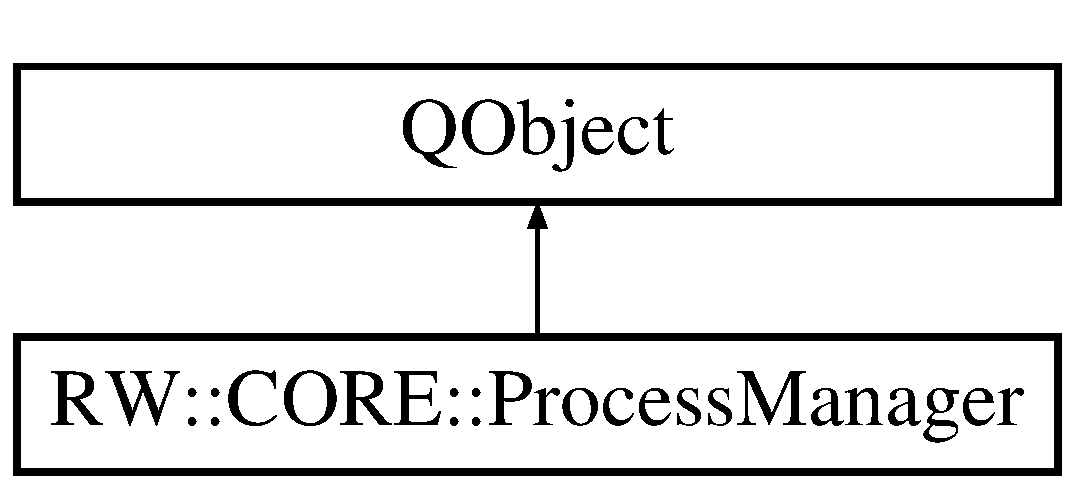
\includegraphics[height=2.000000cm]{class_r_w_1_1_c_o_r_e_1_1_process_manager}
\end{center}
\end{figure}
\subsection*{Public Member Functions}
\begin{DoxyCompactItemize}
\item 
\hyperlink{class_r_w_1_1_c_o_r_e_1_1_process_manager_adca4f2b37dd753be8064af3601855703}{Process\+Manager} (Q\+Object $\ast$Parent=nullptr)
\item 
\hyperlink{class_r_w_1_1_c_o_r_e_1_1_process_manager_abea22c7c5150ff7a2dddb353d84d0715}{$\sim$\+Process\+Manager} ()
\end{DoxyCompactItemize}
\subsection*{Private Attributes}
\begin{DoxyCompactItemize}
\item 
\hyperlink{class_r_w_1_1_c_o_r_e_1_1_communication_manager}{Communication\+Manager} $\ast$ \hyperlink{class_r_w_1_1_c_o_r_e_1_1_process_manager_ae2148c7df93ab1533c4d0370fbd7c60a}{m\+\_\+\+Comm\+Manager}
\item 
\hyperlink{class_r_w_1_1_c_o_r_e_1_1_can_easy_wrapper}{Can\+Easy\+Wrapper} $\ast$ \hyperlink{class_r_w_1_1_c_o_r_e_1_1_process_manager_a18728a50d6e8ee518aaa30656fb6c666}{m\+\_\+\+Can\+Easy}
\item 
\hyperlink{class_r_w_1_1_c_o_r_e_1_1_m_k_s_wrapper}{M\+K\+S\+Wrapper} $\ast$ \hyperlink{class_r_w_1_1_c_o_r_e_1_1_process_manager_a42e601b8fb2073846b13fb0b5fcb6d1a}{m\+\_\+\+M\+KS}
\item 
\hyperlink{class_r_w_1_1_c_o_r_e_1_1_f_host_sp_wrapper}{F\+Host\+Sp\+Wrapper} $\ast$ \hyperlink{class_r_w_1_1_c_o_r_e_1_1_process_manager_aa4122a26664468838c764c93532740fa}{m\+\_\+\+F\+Host\+SP}
\item 
\hyperlink{class_r_w_1_1_c_o_r_e_1_1_portal_info}{Portal\+Info} $\ast$ \hyperlink{class_r_w_1_1_c_o_r_e_1_1_process_manager_aba833f8c7003590a66ff6118fa2cc86d}{m\+\_\+\+Portal\+Info}
\item 
\hyperlink{class_r_w_1_1_c_o_r_e_1_1_error_handler}{Error\+Handler} $\ast$ \hyperlink{class_r_w_1_1_c_o_r_e_1_1_process_manager_ab3bb733bfe0da01794bd4b8674ff8ef9}{m\+\_\+\+Error\+Handler}
\end{DoxyCompactItemize}


\subsection{Detailed Description}


Definition at line 14 of file Process\+Manager.\+h.



\subsection{Constructor \& Destructor Documentation}
\hypertarget{class_r_w_1_1_c_o_r_e_1_1_process_manager_adca4f2b37dd753be8064af3601855703}{}\label{class_r_w_1_1_c_o_r_e_1_1_process_manager_adca4f2b37dd753be8064af3601855703} 
\index{R\+W\+::\+C\+O\+R\+E\+::\+Process\+Manager@{R\+W\+::\+C\+O\+R\+E\+::\+Process\+Manager}!Process\+Manager@{Process\+Manager}}
\index{Process\+Manager@{Process\+Manager}!R\+W\+::\+C\+O\+R\+E\+::\+Process\+Manager@{R\+W\+::\+C\+O\+R\+E\+::\+Process\+Manager}}
\subsubsection{\texorpdfstring{Process\+Manager()}{ProcessManager()}}
{\footnotesize\ttfamily R\+W\+::\+C\+O\+R\+E\+::\+Process\+Manager\+::\+Process\+Manager (\begin{DoxyParamCaption}\item[{Q\+Object $\ast$}]{Parent = {\ttfamily nullptr} }\end{DoxyParamCaption})}



Definition at line 13 of file Process\+Manager.\+cpp.

\hypertarget{class_r_w_1_1_c_o_r_e_1_1_process_manager_abea22c7c5150ff7a2dddb353d84d0715}{}\label{class_r_w_1_1_c_o_r_e_1_1_process_manager_abea22c7c5150ff7a2dddb353d84d0715} 
\index{R\+W\+::\+C\+O\+R\+E\+::\+Process\+Manager@{R\+W\+::\+C\+O\+R\+E\+::\+Process\+Manager}!````~Process\+Manager@{$\sim$\+Process\+Manager}}
\index{````~Process\+Manager@{$\sim$\+Process\+Manager}!R\+W\+::\+C\+O\+R\+E\+::\+Process\+Manager@{R\+W\+::\+C\+O\+R\+E\+::\+Process\+Manager}}
\subsubsection{\texorpdfstring{$\sim$\+Process\+Manager()}{~ProcessManager()}}
{\footnotesize\ttfamily R\+W\+::\+C\+O\+R\+E\+::\+Process\+Manager\+::$\sim$\+Process\+Manager (\begin{DoxyParamCaption}{ }\end{DoxyParamCaption})}



Definition at line 45 of file Process\+Manager.\+cpp.



\subsection{Member Data Documentation}
\hypertarget{class_r_w_1_1_c_o_r_e_1_1_process_manager_a18728a50d6e8ee518aaa30656fb6c666}{}\label{class_r_w_1_1_c_o_r_e_1_1_process_manager_a18728a50d6e8ee518aaa30656fb6c666} 
\index{R\+W\+::\+C\+O\+R\+E\+::\+Process\+Manager@{R\+W\+::\+C\+O\+R\+E\+::\+Process\+Manager}!m\+\_\+\+Can\+Easy@{m\+\_\+\+Can\+Easy}}
\index{m\+\_\+\+Can\+Easy@{m\+\_\+\+Can\+Easy}!R\+W\+::\+C\+O\+R\+E\+::\+Process\+Manager@{R\+W\+::\+C\+O\+R\+E\+::\+Process\+Manager}}
\subsubsection{\texorpdfstring{m\+\_\+\+Can\+Easy}{m\_CanEasy}}
{\footnotesize\ttfamily \hyperlink{class_r_w_1_1_c_o_r_e_1_1_can_easy_wrapper}{Can\+Easy\+Wrapper}$\ast$ R\+W\+::\+C\+O\+R\+E\+::\+Process\+Manager\+::m\+\_\+\+Can\+Easy\hspace{0.3cm}{\ttfamily [private]}}



Definition at line 20 of file Process\+Manager.\+h.

\hypertarget{class_r_w_1_1_c_o_r_e_1_1_process_manager_ae2148c7df93ab1533c4d0370fbd7c60a}{}\label{class_r_w_1_1_c_o_r_e_1_1_process_manager_ae2148c7df93ab1533c4d0370fbd7c60a} 
\index{R\+W\+::\+C\+O\+R\+E\+::\+Process\+Manager@{R\+W\+::\+C\+O\+R\+E\+::\+Process\+Manager}!m\+\_\+\+Comm\+Manager@{m\+\_\+\+Comm\+Manager}}
\index{m\+\_\+\+Comm\+Manager@{m\+\_\+\+Comm\+Manager}!R\+W\+::\+C\+O\+R\+E\+::\+Process\+Manager@{R\+W\+::\+C\+O\+R\+E\+::\+Process\+Manager}}
\subsubsection{\texorpdfstring{m\+\_\+\+Comm\+Manager}{m\_CommManager}}
{\footnotesize\ttfamily \hyperlink{class_r_w_1_1_c_o_r_e_1_1_communication_manager}{Communication\+Manager}$\ast$ R\+W\+::\+C\+O\+R\+E\+::\+Process\+Manager\+::m\+\_\+\+Comm\+Manager\hspace{0.3cm}{\ttfamily [private]}}



Definition at line 19 of file Process\+Manager.\+h.

\hypertarget{class_r_w_1_1_c_o_r_e_1_1_process_manager_ab3bb733bfe0da01794bd4b8674ff8ef9}{}\label{class_r_w_1_1_c_o_r_e_1_1_process_manager_ab3bb733bfe0da01794bd4b8674ff8ef9} 
\index{R\+W\+::\+C\+O\+R\+E\+::\+Process\+Manager@{R\+W\+::\+C\+O\+R\+E\+::\+Process\+Manager}!m\+\_\+\+Error\+Handler@{m\+\_\+\+Error\+Handler}}
\index{m\+\_\+\+Error\+Handler@{m\+\_\+\+Error\+Handler}!R\+W\+::\+C\+O\+R\+E\+::\+Process\+Manager@{R\+W\+::\+C\+O\+R\+E\+::\+Process\+Manager}}
\subsubsection{\texorpdfstring{m\+\_\+\+Error\+Handler}{m\_ErrorHandler}}
{\footnotesize\ttfamily \hyperlink{class_r_w_1_1_c_o_r_e_1_1_error_handler}{Error\+Handler}$\ast$ R\+W\+::\+C\+O\+R\+E\+::\+Process\+Manager\+::m\+\_\+\+Error\+Handler\hspace{0.3cm}{\ttfamily [private]}}



Definition at line 24 of file Process\+Manager.\+h.

\hypertarget{class_r_w_1_1_c_o_r_e_1_1_process_manager_aa4122a26664468838c764c93532740fa}{}\label{class_r_w_1_1_c_o_r_e_1_1_process_manager_aa4122a26664468838c764c93532740fa} 
\index{R\+W\+::\+C\+O\+R\+E\+::\+Process\+Manager@{R\+W\+::\+C\+O\+R\+E\+::\+Process\+Manager}!m\+\_\+\+F\+Host\+SP@{m\+\_\+\+F\+Host\+SP}}
\index{m\+\_\+\+F\+Host\+SP@{m\+\_\+\+F\+Host\+SP}!R\+W\+::\+C\+O\+R\+E\+::\+Process\+Manager@{R\+W\+::\+C\+O\+R\+E\+::\+Process\+Manager}}
\subsubsection{\texorpdfstring{m\+\_\+\+F\+Host\+SP}{m\_FHostSP}}
{\footnotesize\ttfamily \hyperlink{class_r_w_1_1_c_o_r_e_1_1_f_host_sp_wrapper}{F\+Host\+Sp\+Wrapper}$\ast$ R\+W\+::\+C\+O\+R\+E\+::\+Process\+Manager\+::m\+\_\+\+F\+Host\+SP\hspace{0.3cm}{\ttfamily [private]}}



Definition at line 22 of file Process\+Manager.\+h.

\hypertarget{class_r_w_1_1_c_o_r_e_1_1_process_manager_a42e601b8fb2073846b13fb0b5fcb6d1a}{}\label{class_r_w_1_1_c_o_r_e_1_1_process_manager_a42e601b8fb2073846b13fb0b5fcb6d1a} 
\index{R\+W\+::\+C\+O\+R\+E\+::\+Process\+Manager@{R\+W\+::\+C\+O\+R\+E\+::\+Process\+Manager}!m\+\_\+\+M\+KS@{m\+\_\+\+M\+KS}}
\index{m\+\_\+\+M\+KS@{m\+\_\+\+M\+KS}!R\+W\+::\+C\+O\+R\+E\+::\+Process\+Manager@{R\+W\+::\+C\+O\+R\+E\+::\+Process\+Manager}}
\subsubsection{\texorpdfstring{m\+\_\+\+M\+KS}{m\_MKS}}
{\footnotesize\ttfamily \hyperlink{class_r_w_1_1_c_o_r_e_1_1_m_k_s_wrapper}{M\+K\+S\+Wrapper}$\ast$ R\+W\+::\+C\+O\+R\+E\+::\+Process\+Manager\+::m\+\_\+\+M\+KS\hspace{0.3cm}{\ttfamily [private]}}



Definition at line 21 of file Process\+Manager.\+h.

\hypertarget{class_r_w_1_1_c_o_r_e_1_1_process_manager_aba833f8c7003590a66ff6118fa2cc86d}{}\label{class_r_w_1_1_c_o_r_e_1_1_process_manager_aba833f8c7003590a66ff6118fa2cc86d} 
\index{R\+W\+::\+C\+O\+R\+E\+::\+Process\+Manager@{R\+W\+::\+C\+O\+R\+E\+::\+Process\+Manager}!m\+\_\+\+Portal\+Info@{m\+\_\+\+Portal\+Info}}
\index{m\+\_\+\+Portal\+Info@{m\+\_\+\+Portal\+Info}!R\+W\+::\+C\+O\+R\+E\+::\+Process\+Manager@{R\+W\+::\+C\+O\+R\+E\+::\+Process\+Manager}}
\subsubsection{\texorpdfstring{m\+\_\+\+Portal\+Info}{m\_PortalInfo}}
{\footnotesize\ttfamily \hyperlink{class_r_w_1_1_c_o_r_e_1_1_portal_info}{Portal\+Info}$\ast$ R\+W\+::\+C\+O\+R\+E\+::\+Process\+Manager\+::m\+\_\+\+Portal\+Info\hspace{0.3cm}{\ttfamily [private]}}



Definition at line 23 of file Process\+Manager.\+h.



The documentation for this class was generated from the following files\+:\begin{DoxyCompactItemize}
\item 
C\+:/\+Projekte/\+Remote\+Repros/\+Remote\+Hidden\+Helper/\+Remote\+Hidden\+Helper/\hyperlink{_process_manager_8h}{Process\+Manager.\+h}\item 
C\+:/\+Projekte/\+Remote\+Repros/\+Remote\+Hidden\+Helper/\+Remote\+Hidden\+Helper/\hyperlink{_process_manager_8cpp}{Process\+Manager.\+cpp}\end{DoxyCompactItemize}

\hypertarget{structqt__meta__stringdata___dialog_window__t}{}\section{qt\+\_\+meta\+\_\+stringdata\+\_\+\+Dialog\+Window\+\_\+t Struct Reference}
\label{structqt__meta__stringdata___dialog_window__t}\index{qt\+\_\+meta\+\_\+stringdata\+\_\+\+Dialog\+Window\+\_\+t@{qt\+\_\+meta\+\_\+stringdata\+\_\+\+Dialog\+Window\+\_\+t}}
\subsection*{Public Attributes}
\begin{DoxyCompactItemize}
\item 
Q\+Byte\+Array\+Data \hyperlink{structqt__meta__stringdata___dialog_window__t_aa6040f5f9641bf00d019744df4b671d8}{data} \mbox{[}1\mbox{]}
\item 
char \hyperlink{structqt__meta__stringdata___dialog_window__t_a4125b0e6f5ad0b8b506d3296217a3b5b}{stringdata0} \mbox{[}13\mbox{]}
\end{DoxyCompactItemize}


\subsection{Detailed Description}


Definition at line 21 of file moc\+\_\+\+Dialog\+Window.\+cpp.



\subsection{Member Data Documentation}
\hypertarget{structqt__meta__stringdata___dialog_window__t_aa6040f5f9641bf00d019744df4b671d8}{}\label{structqt__meta__stringdata___dialog_window__t_aa6040f5f9641bf00d019744df4b671d8} 
\index{qt\+\_\+meta\+\_\+stringdata\+\_\+\+Dialog\+Window\+\_\+t@{qt\+\_\+meta\+\_\+stringdata\+\_\+\+Dialog\+Window\+\_\+t}!data@{data}}
\index{data@{data}!qt\+\_\+meta\+\_\+stringdata\+\_\+\+Dialog\+Window\+\_\+t@{qt\+\_\+meta\+\_\+stringdata\+\_\+\+Dialog\+Window\+\_\+t}}
\subsubsection{\texorpdfstring{data}{data}}
{\footnotesize\ttfamily Q\+Byte\+Array\+Data qt\+\_\+meta\+\_\+stringdata\+\_\+\+Dialog\+Window\+\_\+t\+::data\mbox{[}1\mbox{]}}



Definition at line 22 of file moc\+\_\+\+Dialog\+Window.\+cpp.

\hypertarget{structqt__meta__stringdata___dialog_window__t_a4125b0e6f5ad0b8b506d3296217a3b5b}{}\label{structqt__meta__stringdata___dialog_window__t_a4125b0e6f5ad0b8b506d3296217a3b5b} 
\index{qt\+\_\+meta\+\_\+stringdata\+\_\+\+Dialog\+Window\+\_\+t@{qt\+\_\+meta\+\_\+stringdata\+\_\+\+Dialog\+Window\+\_\+t}!stringdata0@{stringdata0}}
\index{stringdata0@{stringdata0}!qt\+\_\+meta\+\_\+stringdata\+\_\+\+Dialog\+Window\+\_\+t@{qt\+\_\+meta\+\_\+stringdata\+\_\+\+Dialog\+Window\+\_\+t}}
\subsubsection{\texorpdfstring{stringdata0}{stringdata0}}
{\footnotesize\ttfamily char qt\+\_\+meta\+\_\+stringdata\+\_\+\+Dialog\+Window\+\_\+t\+::stringdata0\mbox{[}13\mbox{]}}



Definition at line 23 of file moc\+\_\+\+Dialog\+Window.\+cpp.



The documentation for this struct was generated from the following file\+:\begin{DoxyCompactItemize}
\item 
C\+:/\+Projekte/\+Remote\+Repros/\+Remote\+Hidden\+Helper/\+Remote\+Hidden\+Helper/\+Generated\+Files/\+Debug/\hyperlink{moc___dialog_window_8cpp}{moc\+\_\+\+Dialog\+Window.\+cpp}\end{DoxyCompactItemize}

\hypertarget{structqt__meta__stringdata___r_w_____c_o_r_e_____basic_wrapper__t}{}\section{qt\+\_\+meta\+\_\+stringdata\+\_\+\+R\+W\+\_\+\+\_\+\+C\+O\+R\+E\+\_\+\+\_\+\+Basic\+Wrapper\+\_\+t Struct Reference}
\label{structqt__meta__stringdata___r_w_____c_o_r_e_____basic_wrapper__t}\index{qt\+\_\+meta\+\_\+stringdata\+\_\+\+R\+W\+\_\+\+\_\+\+C\+O\+R\+E\+\_\+\+\_\+\+Basic\+Wrapper\+\_\+t@{qt\+\_\+meta\+\_\+stringdata\+\_\+\+R\+W\+\_\+\+\_\+\+C\+O\+R\+E\+\_\+\+\_\+\+Basic\+Wrapper\+\_\+t}}
\subsection*{Public Attributes}
\begin{DoxyCompactItemize}
\item 
Q\+Byte\+Array\+Data \hyperlink{structqt__meta__stringdata___r_w_____c_o_r_e_____basic_wrapper__t_a41742c6e1cdccb82ba183c5e5f5d918a}{data} \mbox{[}12\mbox{]}
\item 
char \hyperlink{structqt__meta__stringdata___r_w_____c_o_r_e_____basic_wrapper__t_acfd3e55939192d866ddb55558956a9c6}{stringdata0} \mbox{[}141\mbox{]}
\end{DoxyCompactItemize}


\subsection{Detailed Description}


Definition at line 21 of file moc\+\_\+\+Basic\+Wrapper.\+cpp.



\subsection{Member Data Documentation}
\hypertarget{structqt__meta__stringdata___r_w_____c_o_r_e_____basic_wrapper__t_a41742c6e1cdccb82ba183c5e5f5d918a}{}\label{structqt__meta__stringdata___r_w_____c_o_r_e_____basic_wrapper__t_a41742c6e1cdccb82ba183c5e5f5d918a} 
\index{qt\+\_\+meta\+\_\+stringdata\+\_\+\+R\+W\+\_\+\+\_\+\+C\+O\+R\+E\+\_\+\+\_\+\+Basic\+Wrapper\+\_\+t@{qt\+\_\+meta\+\_\+stringdata\+\_\+\+R\+W\+\_\+\+\_\+\+C\+O\+R\+E\+\_\+\+\_\+\+Basic\+Wrapper\+\_\+t}!data@{data}}
\index{data@{data}!qt\+\_\+meta\+\_\+stringdata\+\_\+\+R\+W\+\_\+\+\_\+\+C\+O\+R\+E\+\_\+\+\_\+\+Basic\+Wrapper\+\_\+t@{qt\+\_\+meta\+\_\+stringdata\+\_\+\+R\+W\+\_\+\+\_\+\+C\+O\+R\+E\+\_\+\+\_\+\+Basic\+Wrapper\+\_\+t}}
\subsubsection{\texorpdfstring{data}{data}}
{\footnotesize\ttfamily Q\+Byte\+Array\+Data qt\+\_\+meta\+\_\+stringdata\+\_\+\+R\+W\+\_\+\+\_\+\+C\+O\+R\+E\+\_\+\+\_\+\+Basic\+Wrapper\+\_\+t\+::data}



Definition at line 22 of file moc\+\_\+\+Basic\+Wrapper.\+cpp.

\hypertarget{structqt__meta__stringdata___r_w_____c_o_r_e_____basic_wrapper__t_acfd3e55939192d866ddb55558956a9c6}{}\label{structqt__meta__stringdata___r_w_____c_o_r_e_____basic_wrapper__t_acfd3e55939192d866ddb55558956a9c6} 
\index{qt\+\_\+meta\+\_\+stringdata\+\_\+\+R\+W\+\_\+\+\_\+\+C\+O\+R\+E\+\_\+\+\_\+\+Basic\+Wrapper\+\_\+t@{qt\+\_\+meta\+\_\+stringdata\+\_\+\+R\+W\+\_\+\+\_\+\+C\+O\+R\+E\+\_\+\+\_\+\+Basic\+Wrapper\+\_\+t}!stringdata0@{stringdata0}}
\index{stringdata0@{stringdata0}!qt\+\_\+meta\+\_\+stringdata\+\_\+\+R\+W\+\_\+\+\_\+\+C\+O\+R\+E\+\_\+\+\_\+\+Basic\+Wrapper\+\_\+t@{qt\+\_\+meta\+\_\+stringdata\+\_\+\+R\+W\+\_\+\+\_\+\+C\+O\+R\+E\+\_\+\+\_\+\+Basic\+Wrapper\+\_\+t}}
\subsubsection{\texorpdfstring{stringdata0}{stringdata0}}
{\footnotesize\ttfamily char qt\+\_\+meta\+\_\+stringdata\+\_\+\+R\+W\+\_\+\+\_\+\+C\+O\+R\+E\+\_\+\+\_\+\+Basic\+Wrapper\+\_\+t\+::stringdata0}



Definition at line 23 of file moc\+\_\+\+Basic\+Wrapper.\+cpp.



The documentation for this struct was generated from the following file\+:\begin{DoxyCompactItemize}
\item 
C\+:/\+Projekte/\+Remote\+Repros/\+Remote\+Hidden\+Helper/\+Remote\+Hidden\+Helper/\+Generated\+Files/\+Debug/\hyperlink{_debug_2moc___basic_wrapper_8cpp}{moc\+\_\+\+Basic\+Wrapper.\+cpp}\end{DoxyCompactItemize}

\hypertarget{structqt__meta__stringdata___r_w_____c_o_r_e_____can_easy_wrapper__t}{}\section{qt\+\_\+meta\+\_\+stringdata\+\_\+\+R\+W\+\_\+\+\_\+\+C\+O\+R\+E\+\_\+\+\_\+\+Can\+Easy\+Wrapper\+\_\+t Struct Reference}
\label{structqt__meta__stringdata___r_w_____c_o_r_e_____can_easy_wrapper__t}\index{qt\+\_\+meta\+\_\+stringdata\+\_\+\+R\+W\+\_\+\+\_\+\+C\+O\+R\+E\+\_\+\+\_\+\+Can\+Easy\+Wrapper\+\_\+t@{qt\+\_\+meta\+\_\+stringdata\+\_\+\+R\+W\+\_\+\+\_\+\+C\+O\+R\+E\+\_\+\+\_\+\+Can\+Easy\+Wrapper\+\_\+t}}
\subsection*{Public Attributes}
\begin{DoxyCompactItemize}
\item 
Q\+Byte\+Array\+Data \hyperlink{structqt__meta__stringdata___r_w_____c_o_r_e_____can_easy_wrapper__t_af8fd7f56e7ad14898aab60bc0f0c60d0}{data} \mbox{[}8\mbox{]}
\item 
char \hyperlink{structqt__meta__stringdata___r_w_____c_o_r_e_____can_easy_wrapper__t_afb65167009a1a69e0769fcae6e2b53f7}{stringdata0} \mbox{[}98\mbox{]}
\end{DoxyCompactItemize}


\subsection{Detailed Description}


Definition at line 21 of file moc\+\_\+\+Can\+Easy\+Wrapper.\+cpp.



\subsection{Member Data Documentation}
\hypertarget{structqt__meta__stringdata___r_w_____c_o_r_e_____can_easy_wrapper__t_af8fd7f56e7ad14898aab60bc0f0c60d0}{}\label{structqt__meta__stringdata___r_w_____c_o_r_e_____can_easy_wrapper__t_af8fd7f56e7ad14898aab60bc0f0c60d0} 
\index{qt\+\_\+meta\+\_\+stringdata\+\_\+\+R\+W\+\_\+\+\_\+\+C\+O\+R\+E\+\_\+\+\_\+\+Can\+Easy\+Wrapper\+\_\+t@{qt\+\_\+meta\+\_\+stringdata\+\_\+\+R\+W\+\_\+\+\_\+\+C\+O\+R\+E\+\_\+\+\_\+\+Can\+Easy\+Wrapper\+\_\+t}!data@{data}}
\index{data@{data}!qt\+\_\+meta\+\_\+stringdata\+\_\+\+R\+W\+\_\+\+\_\+\+C\+O\+R\+E\+\_\+\+\_\+\+Can\+Easy\+Wrapper\+\_\+t@{qt\+\_\+meta\+\_\+stringdata\+\_\+\+R\+W\+\_\+\+\_\+\+C\+O\+R\+E\+\_\+\+\_\+\+Can\+Easy\+Wrapper\+\_\+t}}
\subsubsection{\texorpdfstring{data}{data}}
{\footnotesize\ttfamily Q\+Byte\+Array\+Data qt\+\_\+meta\+\_\+stringdata\+\_\+\+R\+W\+\_\+\+\_\+\+C\+O\+R\+E\+\_\+\+\_\+\+Can\+Easy\+Wrapper\+\_\+t\+::data}



Definition at line 22 of file moc\+\_\+\+Can\+Easy\+Wrapper.\+cpp.

\hypertarget{structqt__meta__stringdata___r_w_____c_o_r_e_____can_easy_wrapper__t_afb65167009a1a69e0769fcae6e2b53f7}{}\label{structqt__meta__stringdata___r_w_____c_o_r_e_____can_easy_wrapper__t_afb65167009a1a69e0769fcae6e2b53f7} 
\index{qt\+\_\+meta\+\_\+stringdata\+\_\+\+R\+W\+\_\+\+\_\+\+C\+O\+R\+E\+\_\+\+\_\+\+Can\+Easy\+Wrapper\+\_\+t@{qt\+\_\+meta\+\_\+stringdata\+\_\+\+R\+W\+\_\+\+\_\+\+C\+O\+R\+E\+\_\+\+\_\+\+Can\+Easy\+Wrapper\+\_\+t}!stringdata0@{stringdata0}}
\index{stringdata0@{stringdata0}!qt\+\_\+meta\+\_\+stringdata\+\_\+\+R\+W\+\_\+\+\_\+\+C\+O\+R\+E\+\_\+\+\_\+\+Can\+Easy\+Wrapper\+\_\+t@{qt\+\_\+meta\+\_\+stringdata\+\_\+\+R\+W\+\_\+\+\_\+\+C\+O\+R\+E\+\_\+\+\_\+\+Can\+Easy\+Wrapper\+\_\+t}}
\subsubsection{\texorpdfstring{stringdata0}{stringdata0}}
{\footnotesize\ttfamily char qt\+\_\+meta\+\_\+stringdata\+\_\+\+R\+W\+\_\+\+\_\+\+C\+O\+R\+E\+\_\+\+\_\+\+Can\+Easy\+Wrapper\+\_\+t\+::stringdata0}



Definition at line 23 of file moc\+\_\+\+Can\+Easy\+Wrapper.\+cpp.



The documentation for this struct was generated from the following file\+:\begin{DoxyCompactItemize}
\item 
C\+:/\+Projekte/\+Remote\+Repros/\+Remote\+Hidden\+Helper/\+Remote\+Hidden\+Helper/\+Generated\+Files/\+Debug/\hyperlink{_debug_2moc___can_easy_wrapper_8cpp}{moc\+\_\+\+Can\+Easy\+Wrapper.\+cpp}\end{DoxyCompactItemize}

\hypertarget{structqt__meta__stringdata___r_w_____c_o_r_e_____communication_manager__t}{}\section{qt\+\_\+meta\+\_\+stringdata\+\_\+\+R\+W\+\_\+\+\_\+\+C\+O\+R\+E\+\_\+\+\_\+\+Communication\+Manager\+\_\+t Struct Reference}
\label{structqt__meta__stringdata___r_w_____c_o_r_e_____communication_manager__t}\index{qt\+\_\+meta\+\_\+stringdata\+\_\+\+R\+W\+\_\+\+\_\+\+C\+O\+R\+E\+\_\+\+\_\+\+Communication\+Manager\+\_\+t@{qt\+\_\+meta\+\_\+stringdata\+\_\+\+R\+W\+\_\+\+\_\+\+C\+O\+R\+E\+\_\+\+\_\+\+Communication\+Manager\+\_\+t}}
\subsection*{Public Attributes}
\begin{DoxyCompactItemize}
\item 
Q\+Byte\+Array\+Data \hyperlink{structqt__meta__stringdata___r_w_____c_o_r_e_____communication_manager__t_a4c365a4c4238281a482a4c3f64e28a32}{data} \mbox{[}14\mbox{]}
\item 
char \hyperlink{structqt__meta__stringdata___r_w_____c_o_r_e_____communication_manager__t_a40ff55b6d2465185cd2cf354e48c98d2}{stringdata0} \mbox{[}175\mbox{]}
\end{DoxyCompactItemize}


\subsection{Detailed Description}


Definition at line 21 of file moc\+\_\+\+Communication\+Manager.\+cpp.



\subsection{Member Data Documentation}
\hypertarget{structqt__meta__stringdata___r_w_____c_o_r_e_____communication_manager__t_a4c365a4c4238281a482a4c3f64e28a32}{}\label{structqt__meta__stringdata___r_w_____c_o_r_e_____communication_manager__t_a4c365a4c4238281a482a4c3f64e28a32} 
\index{qt\+\_\+meta\+\_\+stringdata\+\_\+\+R\+W\+\_\+\+\_\+\+C\+O\+R\+E\+\_\+\+\_\+\+Communication\+Manager\+\_\+t@{qt\+\_\+meta\+\_\+stringdata\+\_\+\+R\+W\+\_\+\+\_\+\+C\+O\+R\+E\+\_\+\+\_\+\+Communication\+Manager\+\_\+t}!data@{data}}
\index{data@{data}!qt\+\_\+meta\+\_\+stringdata\+\_\+\+R\+W\+\_\+\+\_\+\+C\+O\+R\+E\+\_\+\+\_\+\+Communication\+Manager\+\_\+t@{qt\+\_\+meta\+\_\+stringdata\+\_\+\+R\+W\+\_\+\+\_\+\+C\+O\+R\+E\+\_\+\+\_\+\+Communication\+Manager\+\_\+t}}
\subsubsection{\texorpdfstring{data}{data}}
{\footnotesize\ttfamily Q\+Byte\+Array\+Data qt\+\_\+meta\+\_\+stringdata\+\_\+\+R\+W\+\_\+\+\_\+\+C\+O\+R\+E\+\_\+\+\_\+\+Communication\+Manager\+\_\+t\+::data}



Definition at line 22 of file moc\+\_\+\+Communication\+Manager.\+cpp.

\hypertarget{structqt__meta__stringdata___r_w_____c_o_r_e_____communication_manager__t_a40ff55b6d2465185cd2cf354e48c98d2}{}\label{structqt__meta__stringdata___r_w_____c_o_r_e_____communication_manager__t_a40ff55b6d2465185cd2cf354e48c98d2} 
\index{qt\+\_\+meta\+\_\+stringdata\+\_\+\+R\+W\+\_\+\+\_\+\+C\+O\+R\+E\+\_\+\+\_\+\+Communication\+Manager\+\_\+t@{qt\+\_\+meta\+\_\+stringdata\+\_\+\+R\+W\+\_\+\+\_\+\+C\+O\+R\+E\+\_\+\+\_\+\+Communication\+Manager\+\_\+t}!stringdata0@{stringdata0}}
\index{stringdata0@{stringdata0}!qt\+\_\+meta\+\_\+stringdata\+\_\+\+R\+W\+\_\+\+\_\+\+C\+O\+R\+E\+\_\+\+\_\+\+Communication\+Manager\+\_\+t@{qt\+\_\+meta\+\_\+stringdata\+\_\+\+R\+W\+\_\+\+\_\+\+C\+O\+R\+E\+\_\+\+\_\+\+Communication\+Manager\+\_\+t}}
\subsubsection{\texorpdfstring{stringdata0}{stringdata0}}
{\footnotesize\ttfamily char qt\+\_\+meta\+\_\+stringdata\+\_\+\+R\+W\+\_\+\+\_\+\+C\+O\+R\+E\+\_\+\+\_\+\+Communication\+Manager\+\_\+t\+::stringdata0}



Definition at line 23 of file moc\+\_\+\+Communication\+Manager.\+cpp.



The documentation for this struct was generated from the following file\+:\begin{DoxyCompactItemize}
\item 
C\+:/\+Projekte/\+Remote\+Repros/\+Remote\+Hidden\+Helper/\+Remote\+Hidden\+Helper/\+Generated\+Files/\+Debug/\hyperlink{_debug_2moc___communication_manager_8cpp}{moc\+\_\+\+Communication\+Manager.\+cpp}\end{DoxyCompactItemize}

\hypertarget{structqt__meta__stringdata___r_w_____c_o_r_e_____communication_server__t}{}\section{qt\+\_\+meta\+\_\+stringdata\+\_\+\+R\+W\+\_\+\+\_\+\+C\+O\+R\+E\+\_\+\+\_\+\+Communication\+Server\+\_\+t Struct Reference}
\label{structqt__meta__stringdata___r_w_____c_o_r_e_____communication_server__t}\index{qt\+\_\+meta\+\_\+stringdata\+\_\+\+R\+W\+\_\+\+\_\+\+C\+O\+R\+E\+\_\+\+\_\+\+Communication\+Server\+\_\+t@{qt\+\_\+meta\+\_\+stringdata\+\_\+\+R\+W\+\_\+\+\_\+\+C\+O\+R\+E\+\_\+\+\_\+\+Communication\+Server\+\_\+t}}
\subsection*{Public Attributes}
\begin{DoxyCompactItemize}
\item 
Q\+Byte\+Array\+Data \hyperlink{structqt__meta__stringdata___r_w_____c_o_r_e_____communication_server__t_a148f2883b6139a510eb3143b18d3d78b}{data} \mbox{[}10\mbox{]}
\item 
char \hyperlink{structqt__meta__stringdata___r_w_____c_o_r_e_____communication_server__t_acf15bb0f0d6b7cf64db912d68f91c534}{stringdata0} \mbox{[}127\mbox{]}
\end{DoxyCompactItemize}


\subsection{Detailed Description}


Definition at line 21 of file moc\+\_\+\+Communication\+Server.\+cpp.



\subsection{Member Data Documentation}
\hypertarget{structqt__meta__stringdata___r_w_____c_o_r_e_____communication_server__t_a148f2883b6139a510eb3143b18d3d78b}{}\label{structqt__meta__stringdata___r_w_____c_o_r_e_____communication_server__t_a148f2883b6139a510eb3143b18d3d78b} 
\index{qt\+\_\+meta\+\_\+stringdata\+\_\+\+R\+W\+\_\+\+\_\+\+C\+O\+R\+E\+\_\+\+\_\+\+Communication\+Server\+\_\+t@{qt\+\_\+meta\+\_\+stringdata\+\_\+\+R\+W\+\_\+\+\_\+\+C\+O\+R\+E\+\_\+\+\_\+\+Communication\+Server\+\_\+t}!data@{data}}
\index{data@{data}!qt\+\_\+meta\+\_\+stringdata\+\_\+\+R\+W\+\_\+\+\_\+\+C\+O\+R\+E\+\_\+\+\_\+\+Communication\+Server\+\_\+t@{qt\+\_\+meta\+\_\+stringdata\+\_\+\+R\+W\+\_\+\+\_\+\+C\+O\+R\+E\+\_\+\+\_\+\+Communication\+Server\+\_\+t}}
\subsubsection{\texorpdfstring{data}{data}}
{\footnotesize\ttfamily Q\+Byte\+Array\+Data qt\+\_\+meta\+\_\+stringdata\+\_\+\+R\+W\+\_\+\+\_\+\+C\+O\+R\+E\+\_\+\+\_\+\+Communication\+Server\+\_\+t\+::data}



Definition at line 22 of file moc\+\_\+\+Communication\+Server.\+cpp.

\hypertarget{structqt__meta__stringdata___r_w_____c_o_r_e_____communication_server__t_acf15bb0f0d6b7cf64db912d68f91c534}{}\label{structqt__meta__stringdata___r_w_____c_o_r_e_____communication_server__t_acf15bb0f0d6b7cf64db912d68f91c534} 
\index{qt\+\_\+meta\+\_\+stringdata\+\_\+\+R\+W\+\_\+\+\_\+\+C\+O\+R\+E\+\_\+\+\_\+\+Communication\+Server\+\_\+t@{qt\+\_\+meta\+\_\+stringdata\+\_\+\+R\+W\+\_\+\+\_\+\+C\+O\+R\+E\+\_\+\+\_\+\+Communication\+Server\+\_\+t}!stringdata0@{stringdata0}}
\index{stringdata0@{stringdata0}!qt\+\_\+meta\+\_\+stringdata\+\_\+\+R\+W\+\_\+\+\_\+\+C\+O\+R\+E\+\_\+\+\_\+\+Communication\+Server\+\_\+t@{qt\+\_\+meta\+\_\+stringdata\+\_\+\+R\+W\+\_\+\+\_\+\+C\+O\+R\+E\+\_\+\+\_\+\+Communication\+Server\+\_\+t}}
\subsubsection{\texorpdfstring{stringdata0}{stringdata0}}
{\footnotesize\ttfamily char qt\+\_\+meta\+\_\+stringdata\+\_\+\+R\+W\+\_\+\+\_\+\+C\+O\+R\+E\+\_\+\+\_\+\+Communication\+Server\+\_\+t\+::stringdata0}



Definition at line 23 of file moc\+\_\+\+Communication\+Server.\+cpp.



The documentation for this struct was generated from the following file\+:\begin{DoxyCompactItemize}
\item 
C\+:/\+Projekte/\+Remote\+Repros/\+Remote\+Hidden\+Helper/\+Remote\+Hidden\+Helper/\+Generated\+Files/\+Debug/\hyperlink{_debug_2moc___communication_server_8cpp}{moc\+\_\+\+Communication\+Server.\+cpp}\end{DoxyCompactItemize}

\hypertarget{structqt__meta__stringdata___r_w_____c_o_r_e_____error_handler__t}{}\section{qt\+\_\+meta\+\_\+stringdata\+\_\+\+R\+W\+\_\+\+\_\+\+C\+O\+R\+E\+\_\+\+\_\+\+Error\+Handler\+\_\+t Struct Reference}
\label{structqt__meta__stringdata___r_w_____c_o_r_e_____error_handler__t}\index{qt\+\_\+meta\+\_\+stringdata\+\_\+\+R\+W\+\_\+\+\_\+\+C\+O\+R\+E\+\_\+\+\_\+\+Error\+Handler\+\_\+t@{qt\+\_\+meta\+\_\+stringdata\+\_\+\+R\+W\+\_\+\+\_\+\+C\+O\+R\+E\+\_\+\+\_\+\+Error\+Handler\+\_\+t}}
\subsection*{Public Attributes}
\begin{DoxyCompactItemize}
\item 
Q\+Byte\+Array\+Data \hyperlink{structqt__meta__stringdata___r_w_____c_o_r_e_____error_handler__t_a26c0366a4190b24d626ab561f774dd94}{data} \mbox{[}12\mbox{]}
\item 
char \hyperlink{structqt__meta__stringdata___r_w_____c_o_r_e_____error_handler__t_a89162feda77830216ace7a3f2523f5ad}{stringdata0} \mbox{[}147\mbox{]}
\end{DoxyCompactItemize}


\subsection{Detailed Description}


Definition at line 21 of file moc\+\_\+\+Error\+Handler.\+cpp.



\subsection{Member Data Documentation}
\hypertarget{structqt__meta__stringdata___r_w_____c_o_r_e_____error_handler__t_a26c0366a4190b24d626ab561f774dd94}{}\label{structqt__meta__stringdata___r_w_____c_o_r_e_____error_handler__t_a26c0366a4190b24d626ab561f774dd94} 
\index{qt\+\_\+meta\+\_\+stringdata\+\_\+\+R\+W\+\_\+\+\_\+\+C\+O\+R\+E\+\_\+\+\_\+\+Error\+Handler\+\_\+t@{qt\+\_\+meta\+\_\+stringdata\+\_\+\+R\+W\+\_\+\+\_\+\+C\+O\+R\+E\+\_\+\+\_\+\+Error\+Handler\+\_\+t}!data@{data}}
\index{data@{data}!qt\+\_\+meta\+\_\+stringdata\+\_\+\+R\+W\+\_\+\+\_\+\+C\+O\+R\+E\+\_\+\+\_\+\+Error\+Handler\+\_\+t@{qt\+\_\+meta\+\_\+stringdata\+\_\+\+R\+W\+\_\+\+\_\+\+C\+O\+R\+E\+\_\+\+\_\+\+Error\+Handler\+\_\+t}}
\subsubsection{\texorpdfstring{data}{data}}
{\footnotesize\ttfamily Q\+Byte\+Array\+Data qt\+\_\+meta\+\_\+stringdata\+\_\+\+R\+W\+\_\+\+\_\+\+C\+O\+R\+E\+\_\+\+\_\+\+Error\+Handler\+\_\+t\+::data\mbox{[}12\mbox{]}}



Definition at line 22 of file moc\+\_\+\+Error\+Handler.\+cpp.

\hypertarget{structqt__meta__stringdata___r_w_____c_o_r_e_____error_handler__t_a89162feda77830216ace7a3f2523f5ad}{}\label{structqt__meta__stringdata___r_w_____c_o_r_e_____error_handler__t_a89162feda77830216ace7a3f2523f5ad} 
\index{qt\+\_\+meta\+\_\+stringdata\+\_\+\+R\+W\+\_\+\+\_\+\+C\+O\+R\+E\+\_\+\+\_\+\+Error\+Handler\+\_\+t@{qt\+\_\+meta\+\_\+stringdata\+\_\+\+R\+W\+\_\+\+\_\+\+C\+O\+R\+E\+\_\+\+\_\+\+Error\+Handler\+\_\+t}!stringdata0@{stringdata0}}
\index{stringdata0@{stringdata0}!qt\+\_\+meta\+\_\+stringdata\+\_\+\+R\+W\+\_\+\+\_\+\+C\+O\+R\+E\+\_\+\+\_\+\+Error\+Handler\+\_\+t@{qt\+\_\+meta\+\_\+stringdata\+\_\+\+R\+W\+\_\+\+\_\+\+C\+O\+R\+E\+\_\+\+\_\+\+Error\+Handler\+\_\+t}}
\subsubsection{\texorpdfstring{stringdata0}{stringdata0}}
{\footnotesize\ttfamily char qt\+\_\+meta\+\_\+stringdata\+\_\+\+R\+W\+\_\+\+\_\+\+C\+O\+R\+E\+\_\+\+\_\+\+Error\+Handler\+\_\+t\+::stringdata0\mbox{[}147\mbox{]}}



Definition at line 23 of file moc\+\_\+\+Error\+Handler.\+cpp.



The documentation for this struct was generated from the following file\+:\begin{DoxyCompactItemize}
\item 
C\+:/\+Projekte/\+Remote\+Repros/\+Remote\+Hidden\+Helper/\+Remote\+Hidden\+Helper/\+Generated\+Files/\+Debug/\hyperlink{moc___error_handler_8cpp}{moc\+\_\+\+Error\+Handler.\+cpp}\end{DoxyCompactItemize}

\hypertarget{structqt__meta__stringdata___r_w_____c_o_r_e_____f_host_sp_wrapper__t}{}\section{qt\+\_\+meta\+\_\+stringdata\+\_\+\+R\+W\+\_\+\+\_\+\+C\+O\+R\+E\+\_\+\+\_\+\+F\+Host\+Sp\+Wrapper\+\_\+t Struct Reference}
\label{structqt__meta__stringdata___r_w_____c_o_r_e_____f_host_sp_wrapper__t}\index{qt\+\_\+meta\+\_\+stringdata\+\_\+\+R\+W\+\_\+\+\_\+\+C\+O\+R\+E\+\_\+\+\_\+\+F\+Host\+Sp\+Wrapper\+\_\+t@{qt\+\_\+meta\+\_\+stringdata\+\_\+\+R\+W\+\_\+\+\_\+\+C\+O\+R\+E\+\_\+\+\_\+\+F\+Host\+Sp\+Wrapper\+\_\+t}}
\subsection*{Public Attributes}
\begin{DoxyCompactItemize}
\item 
Q\+Byte\+Array\+Data \hyperlink{structqt__meta__stringdata___r_w_____c_o_r_e_____f_host_sp_wrapper__t_aae021c0f6e31cd9a2ea438476facc0ee}{data} \mbox{[}8\mbox{]}
\item 
char \hyperlink{structqt__meta__stringdata___r_w_____c_o_r_e_____f_host_sp_wrapper__t_a9d1313b4195bca5e48e5fba152725df4}{stringdata0} \mbox{[}98\mbox{]}
\end{DoxyCompactItemize}


\subsection{Detailed Description}


Definition at line 21 of file moc\+\_\+\+F\+Host\+Sp\+Wrapper.\+cpp.



\subsection{Member Data Documentation}
\hypertarget{structqt__meta__stringdata___r_w_____c_o_r_e_____f_host_sp_wrapper__t_aae021c0f6e31cd9a2ea438476facc0ee}{}\label{structqt__meta__stringdata___r_w_____c_o_r_e_____f_host_sp_wrapper__t_aae021c0f6e31cd9a2ea438476facc0ee} 
\index{qt\+\_\+meta\+\_\+stringdata\+\_\+\+R\+W\+\_\+\+\_\+\+C\+O\+R\+E\+\_\+\+\_\+\+F\+Host\+Sp\+Wrapper\+\_\+t@{qt\+\_\+meta\+\_\+stringdata\+\_\+\+R\+W\+\_\+\+\_\+\+C\+O\+R\+E\+\_\+\+\_\+\+F\+Host\+Sp\+Wrapper\+\_\+t}!data@{data}}
\index{data@{data}!qt\+\_\+meta\+\_\+stringdata\+\_\+\+R\+W\+\_\+\+\_\+\+C\+O\+R\+E\+\_\+\+\_\+\+F\+Host\+Sp\+Wrapper\+\_\+t@{qt\+\_\+meta\+\_\+stringdata\+\_\+\+R\+W\+\_\+\+\_\+\+C\+O\+R\+E\+\_\+\+\_\+\+F\+Host\+Sp\+Wrapper\+\_\+t}}
\subsubsection{\texorpdfstring{data}{data}}
{\footnotesize\ttfamily Q\+Byte\+Array\+Data qt\+\_\+meta\+\_\+stringdata\+\_\+\+R\+W\+\_\+\+\_\+\+C\+O\+R\+E\+\_\+\+\_\+\+F\+Host\+Sp\+Wrapper\+\_\+t\+::data}



Definition at line 22 of file moc\+\_\+\+F\+Host\+Sp\+Wrapper.\+cpp.

\hypertarget{structqt__meta__stringdata___r_w_____c_o_r_e_____f_host_sp_wrapper__t_a9d1313b4195bca5e48e5fba152725df4}{}\label{structqt__meta__stringdata___r_w_____c_o_r_e_____f_host_sp_wrapper__t_a9d1313b4195bca5e48e5fba152725df4} 
\index{qt\+\_\+meta\+\_\+stringdata\+\_\+\+R\+W\+\_\+\+\_\+\+C\+O\+R\+E\+\_\+\+\_\+\+F\+Host\+Sp\+Wrapper\+\_\+t@{qt\+\_\+meta\+\_\+stringdata\+\_\+\+R\+W\+\_\+\+\_\+\+C\+O\+R\+E\+\_\+\+\_\+\+F\+Host\+Sp\+Wrapper\+\_\+t}!stringdata0@{stringdata0}}
\index{stringdata0@{stringdata0}!qt\+\_\+meta\+\_\+stringdata\+\_\+\+R\+W\+\_\+\+\_\+\+C\+O\+R\+E\+\_\+\+\_\+\+F\+Host\+Sp\+Wrapper\+\_\+t@{qt\+\_\+meta\+\_\+stringdata\+\_\+\+R\+W\+\_\+\+\_\+\+C\+O\+R\+E\+\_\+\+\_\+\+F\+Host\+Sp\+Wrapper\+\_\+t}}
\subsubsection{\texorpdfstring{stringdata0}{stringdata0}}
{\footnotesize\ttfamily char qt\+\_\+meta\+\_\+stringdata\+\_\+\+R\+W\+\_\+\+\_\+\+C\+O\+R\+E\+\_\+\+\_\+\+F\+Host\+Sp\+Wrapper\+\_\+t\+::stringdata0}



Definition at line 23 of file moc\+\_\+\+F\+Host\+Sp\+Wrapper.\+cpp.



The documentation for this struct was generated from the following file\+:\begin{DoxyCompactItemize}
\item 
C\+:/\+Projekte/\+Remote\+Repros/\+Remote\+Hidden\+Helper/\+Remote\+Hidden\+Helper/\+Generated\+Files/\+Debug/\hyperlink{_debug_2moc___f_host_sp_wrapper_8cpp}{moc\+\_\+\+F\+Host\+Sp\+Wrapper.\+cpp}\end{DoxyCompactItemize}

\hypertarget{structqt__meta__stringdata___r_w_____c_o_r_e_____m_k_s_wrapper__t}{}\section{qt\+\_\+meta\+\_\+stringdata\+\_\+\+R\+W\+\_\+\+\_\+\+C\+O\+R\+E\+\_\+\+\_\+\+M\+K\+S\+Wrapper\+\_\+t Struct Reference}
\label{structqt__meta__stringdata___r_w_____c_o_r_e_____m_k_s_wrapper__t}\index{qt\+\_\+meta\+\_\+stringdata\+\_\+\+R\+W\+\_\+\+\_\+\+C\+O\+R\+E\+\_\+\+\_\+\+M\+K\+S\+Wrapper\+\_\+t@{qt\+\_\+meta\+\_\+stringdata\+\_\+\+R\+W\+\_\+\+\_\+\+C\+O\+R\+E\+\_\+\+\_\+\+M\+K\+S\+Wrapper\+\_\+t}}
\subsection*{Public Attributes}
\begin{DoxyCompactItemize}
\item 
Q\+Byte\+Array\+Data \hyperlink{structqt__meta__stringdata___r_w_____c_o_r_e_____m_k_s_wrapper__t_a56d1a9154896b56b5b9bfda69f57dce1}{data} \mbox{[}8\mbox{]}
\item 
char \hyperlink{structqt__meta__stringdata___r_w_____c_o_r_e_____m_k_s_wrapper__t_a3e76e021f0d5fc6df11f5a7760ef0411}{stringdata0} \mbox{[}94\mbox{]}
\end{DoxyCompactItemize}


\subsection{Detailed Description}


Definition at line 21 of file moc\+\_\+\+M\+K\+S\+Wrapper.\+cpp.



\subsection{Member Data Documentation}
\hypertarget{structqt__meta__stringdata___r_w_____c_o_r_e_____m_k_s_wrapper__t_a56d1a9154896b56b5b9bfda69f57dce1}{}\label{structqt__meta__stringdata___r_w_____c_o_r_e_____m_k_s_wrapper__t_a56d1a9154896b56b5b9bfda69f57dce1} 
\index{qt\+\_\+meta\+\_\+stringdata\+\_\+\+R\+W\+\_\+\+\_\+\+C\+O\+R\+E\+\_\+\+\_\+\+M\+K\+S\+Wrapper\+\_\+t@{qt\+\_\+meta\+\_\+stringdata\+\_\+\+R\+W\+\_\+\+\_\+\+C\+O\+R\+E\+\_\+\+\_\+\+M\+K\+S\+Wrapper\+\_\+t}!data@{data}}
\index{data@{data}!qt\+\_\+meta\+\_\+stringdata\+\_\+\+R\+W\+\_\+\+\_\+\+C\+O\+R\+E\+\_\+\+\_\+\+M\+K\+S\+Wrapper\+\_\+t@{qt\+\_\+meta\+\_\+stringdata\+\_\+\+R\+W\+\_\+\+\_\+\+C\+O\+R\+E\+\_\+\+\_\+\+M\+K\+S\+Wrapper\+\_\+t}}
\subsubsection{\texorpdfstring{data}{data}}
{\footnotesize\ttfamily Q\+Byte\+Array\+Data qt\+\_\+meta\+\_\+stringdata\+\_\+\+R\+W\+\_\+\+\_\+\+C\+O\+R\+E\+\_\+\+\_\+\+M\+K\+S\+Wrapper\+\_\+t\+::data}



Definition at line 22 of file moc\+\_\+\+M\+K\+S\+Wrapper.\+cpp.

\hypertarget{structqt__meta__stringdata___r_w_____c_o_r_e_____m_k_s_wrapper__t_a3e76e021f0d5fc6df11f5a7760ef0411}{}\label{structqt__meta__stringdata___r_w_____c_o_r_e_____m_k_s_wrapper__t_a3e76e021f0d5fc6df11f5a7760ef0411} 
\index{qt\+\_\+meta\+\_\+stringdata\+\_\+\+R\+W\+\_\+\+\_\+\+C\+O\+R\+E\+\_\+\+\_\+\+M\+K\+S\+Wrapper\+\_\+t@{qt\+\_\+meta\+\_\+stringdata\+\_\+\+R\+W\+\_\+\+\_\+\+C\+O\+R\+E\+\_\+\+\_\+\+M\+K\+S\+Wrapper\+\_\+t}!stringdata0@{stringdata0}}
\index{stringdata0@{stringdata0}!qt\+\_\+meta\+\_\+stringdata\+\_\+\+R\+W\+\_\+\+\_\+\+C\+O\+R\+E\+\_\+\+\_\+\+M\+K\+S\+Wrapper\+\_\+t@{qt\+\_\+meta\+\_\+stringdata\+\_\+\+R\+W\+\_\+\+\_\+\+C\+O\+R\+E\+\_\+\+\_\+\+M\+K\+S\+Wrapper\+\_\+t}}
\subsubsection{\texorpdfstring{stringdata0}{stringdata0}}
{\footnotesize\ttfamily char qt\+\_\+meta\+\_\+stringdata\+\_\+\+R\+W\+\_\+\+\_\+\+C\+O\+R\+E\+\_\+\+\_\+\+M\+K\+S\+Wrapper\+\_\+t\+::stringdata0}



Definition at line 23 of file moc\+\_\+\+M\+K\+S\+Wrapper.\+cpp.



The documentation for this struct was generated from the following file\+:\begin{DoxyCompactItemize}
\item 
C\+:/\+Projekte/\+Remote\+Repros/\+Remote\+Hidden\+Helper/\+Remote\+Hidden\+Helper/\+Generated\+Files/\+Debug/\hyperlink{_debug_2moc___m_k_s_wrapper_8cpp}{moc\+\_\+\+M\+K\+S\+Wrapper.\+cpp}\end{DoxyCompactItemize}

\hypertarget{structqt__meta__stringdata___r_w_____c_o_r_e_____portal_info__t}{}\section{qt\+\_\+meta\+\_\+stringdata\+\_\+\+R\+W\+\_\+\+\_\+\+C\+O\+R\+E\+\_\+\+\_\+\+Portal\+Info\+\_\+t Struct Reference}
\label{structqt__meta__stringdata___r_w_____c_o_r_e_____portal_info__t}\index{qt\+\_\+meta\+\_\+stringdata\+\_\+\+R\+W\+\_\+\+\_\+\+C\+O\+R\+E\+\_\+\+\_\+\+Portal\+Info\+\_\+t@{qt\+\_\+meta\+\_\+stringdata\+\_\+\+R\+W\+\_\+\+\_\+\+C\+O\+R\+E\+\_\+\+\_\+\+Portal\+Info\+\_\+t}}
\subsection*{Public Attributes}
\begin{DoxyCompactItemize}
\item 
Q\+Byte\+Array\+Data \hyperlink{structqt__meta__stringdata___r_w_____c_o_r_e_____portal_info__t_a5c5462c9e400d81ca69701585dcf44c0}{data} \mbox{[}14\mbox{]}
\item 
char \hyperlink{structqt__meta__stringdata___r_w_____c_o_r_e_____portal_info__t_a1ad3d524b97d8b9d7602da3f49431797}{stringdata0} \mbox{[}208\mbox{]}
\end{DoxyCompactItemize}


\subsection{Detailed Description}


Definition at line 21 of file moc\+\_\+\+Portal\+Info.\+cpp.



\subsection{Member Data Documentation}
\hypertarget{structqt__meta__stringdata___r_w_____c_o_r_e_____portal_info__t_a5c5462c9e400d81ca69701585dcf44c0}{}\label{structqt__meta__stringdata___r_w_____c_o_r_e_____portal_info__t_a5c5462c9e400d81ca69701585dcf44c0} 
\index{qt\+\_\+meta\+\_\+stringdata\+\_\+\+R\+W\+\_\+\+\_\+\+C\+O\+R\+E\+\_\+\+\_\+\+Portal\+Info\+\_\+t@{qt\+\_\+meta\+\_\+stringdata\+\_\+\+R\+W\+\_\+\+\_\+\+C\+O\+R\+E\+\_\+\+\_\+\+Portal\+Info\+\_\+t}!data@{data}}
\index{data@{data}!qt\+\_\+meta\+\_\+stringdata\+\_\+\+R\+W\+\_\+\+\_\+\+C\+O\+R\+E\+\_\+\+\_\+\+Portal\+Info\+\_\+t@{qt\+\_\+meta\+\_\+stringdata\+\_\+\+R\+W\+\_\+\+\_\+\+C\+O\+R\+E\+\_\+\+\_\+\+Portal\+Info\+\_\+t}}
\subsubsection{\texorpdfstring{data}{data}}
{\footnotesize\ttfamily Q\+Byte\+Array\+Data qt\+\_\+meta\+\_\+stringdata\+\_\+\+R\+W\+\_\+\+\_\+\+C\+O\+R\+E\+\_\+\+\_\+\+Portal\+Info\+\_\+t\+::data\mbox{[}14\mbox{]}}



Definition at line 22 of file moc\+\_\+\+Portal\+Info.\+cpp.

\hypertarget{structqt__meta__stringdata___r_w_____c_o_r_e_____portal_info__t_a1ad3d524b97d8b9d7602da3f49431797}{}\label{structqt__meta__stringdata___r_w_____c_o_r_e_____portal_info__t_a1ad3d524b97d8b9d7602da3f49431797} 
\index{qt\+\_\+meta\+\_\+stringdata\+\_\+\+R\+W\+\_\+\+\_\+\+C\+O\+R\+E\+\_\+\+\_\+\+Portal\+Info\+\_\+t@{qt\+\_\+meta\+\_\+stringdata\+\_\+\+R\+W\+\_\+\+\_\+\+C\+O\+R\+E\+\_\+\+\_\+\+Portal\+Info\+\_\+t}!stringdata0@{stringdata0}}
\index{stringdata0@{stringdata0}!qt\+\_\+meta\+\_\+stringdata\+\_\+\+R\+W\+\_\+\+\_\+\+C\+O\+R\+E\+\_\+\+\_\+\+Portal\+Info\+\_\+t@{qt\+\_\+meta\+\_\+stringdata\+\_\+\+R\+W\+\_\+\+\_\+\+C\+O\+R\+E\+\_\+\+\_\+\+Portal\+Info\+\_\+t}}
\subsubsection{\texorpdfstring{stringdata0}{stringdata0}}
{\footnotesize\ttfamily char qt\+\_\+meta\+\_\+stringdata\+\_\+\+R\+W\+\_\+\+\_\+\+C\+O\+R\+E\+\_\+\+\_\+\+Portal\+Info\+\_\+t\+::stringdata0\mbox{[}208\mbox{]}}



Definition at line 23 of file moc\+\_\+\+Portal\+Info.\+cpp.



The documentation for this struct was generated from the following file\+:\begin{DoxyCompactItemize}
\item 
C\+:/\+Projekte/\+Remote\+Repros/\+Remote\+Hidden\+Helper/\+Remote\+Hidden\+Helper/\+Generated\+Files/\+Debug/\hyperlink{moc___portal_info_8cpp}{moc\+\_\+\+Portal\+Info.\+cpp}\end{DoxyCompactItemize}

\hypertarget{structqt__meta__stringdata___r_w_____c_o_r_e_____process_manager__t}{}\section{qt\+\_\+meta\+\_\+stringdata\+\_\+\+R\+W\+\_\+\+\_\+\+C\+O\+R\+E\+\_\+\+\_\+\+Process\+Manager\+\_\+t Struct Reference}
\label{structqt__meta__stringdata___r_w_____c_o_r_e_____process_manager__t}\index{qt\+\_\+meta\+\_\+stringdata\+\_\+\+R\+W\+\_\+\+\_\+\+C\+O\+R\+E\+\_\+\+\_\+\+Process\+Manager\+\_\+t@{qt\+\_\+meta\+\_\+stringdata\+\_\+\+R\+W\+\_\+\+\_\+\+C\+O\+R\+E\+\_\+\+\_\+\+Process\+Manager\+\_\+t}}
\subsection*{Public Attributes}
\begin{DoxyCompactItemize}
\item 
Q\+Byte\+Array\+Data \hyperlink{structqt__meta__stringdata___r_w_____c_o_r_e_____process_manager__t_a053b1495564a42f1ca28183ecfa5fb2c}{data} \mbox{[}1\mbox{]}
\item 
char \hyperlink{structqt__meta__stringdata___r_w_____c_o_r_e_____process_manager__t_a2ab1016f5cce35de3db06dd2503c6ead}{stringdata0} \mbox{[}25\mbox{]}
\end{DoxyCompactItemize}


\subsection{Detailed Description}


Definition at line 21 of file moc\+\_\+\+Process\+Manager.\+cpp.



\subsection{Member Data Documentation}
\hypertarget{structqt__meta__stringdata___r_w_____c_o_r_e_____process_manager__t_a053b1495564a42f1ca28183ecfa5fb2c}{}\label{structqt__meta__stringdata___r_w_____c_o_r_e_____process_manager__t_a053b1495564a42f1ca28183ecfa5fb2c} 
\index{qt\+\_\+meta\+\_\+stringdata\+\_\+\+R\+W\+\_\+\+\_\+\+C\+O\+R\+E\+\_\+\+\_\+\+Process\+Manager\+\_\+t@{qt\+\_\+meta\+\_\+stringdata\+\_\+\+R\+W\+\_\+\+\_\+\+C\+O\+R\+E\+\_\+\+\_\+\+Process\+Manager\+\_\+t}!data@{data}}
\index{data@{data}!qt\+\_\+meta\+\_\+stringdata\+\_\+\+R\+W\+\_\+\+\_\+\+C\+O\+R\+E\+\_\+\+\_\+\+Process\+Manager\+\_\+t@{qt\+\_\+meta\+\_\+stringdata\+\_\+\+R\+W\+\_\+\+\_\+\+C\+O\+R\+E\+\_\+\+\_\+\+Process\+Manager\+\_\+t}}
\subsubsection{\texorpdfstring{data}{data}}
{\footnotesize\ttfamily Q\+Byte\+Array\+Data qt\+\_\+meta\+\_\+stringdata\+\_\+\+R\+W\+\_\+\+\_\+\+C\+O\+R\+E\+\_\+\+\_\+\+Process\+Manager\+\_\+t\+::data}



Definition at line 22 of file moc\+\_\+\+Process\+Manager.\+cpp.

\hypertarget{structqt__meta__stringdata___r_w_____c_o_r_e_____process_manager__t_a2ab1016f5cce35de3db06dd2503c6ead}{}\label{structqt__meta__stringdata___r_w_____c_o_r_e_____process_manager__t_a2ab1016f5cce35de3db06dd2503c6ead} 
\index{qt\+\_\+meta\+\_\+stringdata\+\_\+\+R\+W\+\_\+\+\_\+\+C\+O\+R\+E\+\_\+\+\_\+\+Process\+Manager\+\_\+t@{qt\+\_\+meta\+\_\+stringdata\+\_\+\+R\+W\+\_\+\+\_\+\+C\+O\+R\+E\+\_\+\+\_\+\+Process\+Manager\+\_\+t}!stringdata0@{stringdata0}}
\index{stringdata0@{stringdata0}!qt\+\_\+meta\+\_\+stringdata\+\_\+\+R\+W\+\_\+\+\_\+\+C\+O\+R\+E\+\_\+\+\_\+\+Process\+Manager\+\_\+t@{qt\+\_\+meta\+\_\+stringdata\+\_\+\+R\+W\+\_\+\+\_\+\+C\+O\+R\+E\+\_\+\+\_\+\+Process\+Manager\+\_\+t}}
\subsubsection{\texorpdfstring{stringdata0}{stringdata0}}
{\footnotesize\ttfamily char qt\+\_\+meta\+\_\+stringdata\+\_\+\+R\+W\+\_\+\+\_\+\+C\+O\+R\+E\+\_\+\+\_\+\+Process\+Manager\+\_\+t\+::stringdata0}



Definition at line 23 of file moc\+\_\+\+Process\+Manager.\+cpp.



The documentation for this struct was generated from the following file\+:\begin{DoxyCompactItemize}
\item 
C\+:/\+Projekte/\+Remote\+Repros/\+Remote\+Hidden\+Helper/\+Remote\+Hidden\+Helper/\+Generated\+Files/\+Debug/\hyperlink{_debug_2moc___process_manager_8cpp}{moc\+\_\+\+Process\+Manager.\+cpp}\end{DoxyCompactItemize}

\hypertarget{structqt__meta__stringdata___r_w_____c_o_r_e_____remote_hidden_helper__t}{}\section{qt\+\_\+meta\+\_\+stringdata\+\_\+\+R\+W\+\_\+\+\_\+\+C\+O\+R\+E\+\_\+\+\_\+\+Remote\+Hidden\+Helper\+\_\+t Struct Reference}
\label{structqt__meta__stringdata___r_w_____c_o_r_e_____remote_hidden_helper__t}\index{qt\+\_\+meta\+\_\+stringdata\+\_\+\+R\+W\+\_\+\+\_\+\+C\+O\+R\+E\+\_\+\+\_\+\+Remote\+Hidden\+Helper\+\_\+t@{qt\+\_\+meta\+\_\+stringdata\+\_\+\+R\+W\+\_\+\+\_\+\+C\+O\+R\+E\+\_\+\+\_\+\+Remote\+Hidden\+Helper\+\_\+t}}
\subsection*{Public Attributes}
\begin{DoxyCompactItemize}
\item 
Q\+Byte\+Array\+Data \hyperlink{structqt__meta__stringdata___r_w_____c_o_r_e_____remote_hidden_helper__t_a1571560175539826031952b10eb7cb3c}{data} \mbox{[}1\mbox{]}
\item 
char \hyperlink{structqt__meta__stringdata___r_w_____c_o_r_e_____remote_hidden_helper__t_aff520200e964f9c40cd2d329d5b95a97}{stringdata0} \mbox{[}29\mbox{]}
\end{DoxyCompactItemize}


\subsection{Detailed Description}


Definition at line 21 of file moc\+\_\+remotehiddenhelper.\+cpp.



\subsection{Member Data Documentation}
\hypertarget{structqt__meta__stringdata___r_w_____c_o_r_e_____remote_hidden_helper__t_a1571560175539826031952b10eb7cb3c}{}\label{structqt__meta__stringdata___r_w_____c_o_r_e_____remote_hidden_helper__t_a1571560175539826031952b10eb7cb3c} 
\index{qt\+\_\+meta\+\_\+stringdata\+\_\+\+R\+W\+\_\+\+\_\+\+C\+O\+R\+E\+\_\+\+\_\+\+Remote\+Hidden\+Helper\+\_\+t@{qt\+\_\+meta\+\_\+stringdata\+\_\+\+R\+W\+\_\+\+\_\+\+C\+O\+R\+E\+\_\+\+\_\+\+Remote\+Hidden\+Helper\+\_\+t}!data@{data}}
\index{data@{data}!qt\+\_\+meta\+\_\+stringdata\+\_\+\+R\+W\+\_\+\+\_\+\+C\+O\+R\+E\+\_\+\+\_\+\+Remote\+Hidden\+Helper\+\_\+t@{qt\+\_\+meta\+\_\+stringdata\+\_\+\+R\+W\+\_\+\+\_\+\+C\+O\+R\+E\+\_\+\+\_\+\+Remote\+Hidden\+Helper\+\_\+t}}
\subsubsection{\texorpdfstring{data}{data}}
{\footnotesize\ttfamily Q\+Byte\+Array\+Data qt\+\_\+meta\+\_\+stringdata\+\_\+\+R\+W\+\_\+\+\_\+\+C\+O\+R\+E\+\_\+\+\_\+\+Remote\+Hidden\+Helper\+\_\+t\+::data}



Definition at line 22 of file moc\+\_\+remotehiddenhelper.\+cpp.

\hypertarget{structqt__meta__stringdata___r_w_____c_o_r_e_____remote_hidden_helper__t_aff520200e964f9c40cd2d329d5b95a97}{}\label{structqt__meta__stringdata___r_w_____c_o_r_e_____remote_hidden_helper__t_aff520200e964f9c40cd2d329d5b95a97} 
\index{qt\+\_\+meta\+\_\+stringdata\+\_\+\+R\+W\+\_\+\+\_\+\+C\+O\+R\+E\+\_\+\+\_\+\+Remote\+Hidden\+Helper\+\_\+t@{qt\+\_\+meta\+\_\+stringdata\+\_\+\+R\+W\+\_\+\+\_\+\+C\+O\+R\+E\+\_\+\+\_\+\+Remote\+Hidden\+Helper\+\_\+t}!stringdata0@{stringdata0}}
\index{stringdata0@{stringdata0}!qt\+\_\+meta\+\_\+stringdata\+\_\+\+R\+W\+\_\+\+\_\+\+C\+O\+R\+E\+\_\+\+\_\+\+Remote\+Hidden\+Helper\+\_\+t@{qt\+\_\+meta\+\_\+stringdata\+\_\+\+R\+W\+\_\+\+\_\+\+C\+O\+R\+E\+\_\+\+\_\+\+Remote\+Hidden\+Helper\+\_\+t}}
\subsubsection{\texorpdfstring{stringdata0}{stringdata0}}
{\footnotesize\ttfamily char qt\+\_\+meta\+\_\+stringdata\+\_\+\+R\+W\+\_\+\+\_\+\+C\+O\+R\+E\+\_\+\+\_\+\+Remote\+Hidden\+Helper\+\_\+t\+::stringdata0}



Definition at line 23 of file moc\+\_\+remotehiddenhelper.\+cpp.



The documentation for this struct was generated from the following file\+:\begin{DoxyCompactItemize}
\item 
C\+:/\+Projekte/\+Remote\+Repros/\+Remote\+Hidden\+Helper/\+Remote\+Hidden\+Helper/\+Generated\+Files/\+Debug/\hyperlink{_debug_2moc__remotehiddenhelper_8cpp}{moc\+\_\+remotehiddenhelper.\+cpp}\end{DoxyCompactItemize}

\hypertarget{structqt__meta__stringdata___r_w_____c_o_r_e_____unit__t}{}\section{qt\+\_\+meta\+\_\+stringdata\+\_\+\+R\+W\+\_\+\+\_\+\+C\+O\+R\+E\+\_\+\+\_\+\+Unit\+\_\+t Struct Reference}
\label{structqt__meta__stringdata___r_w_____c_o_r_e_____unit__t}\index{qt\+\_\+meta\+\_\+stringdata\+\_\+\+R\+W\+\_\+\+\_\+\+C\+O\+R\+E\+\_\+\+\_\+\+Unit\+\_\+t@{qt\+\_\+meta\+\_\+stringdata\+\_\+\+R\+W\+\_\+\+\_\+\+C\+O\+R\+E\+\_\+\+\_\+\+Unit\+\_\+t}}
\subsection*{Public Attributes}
\begin{DoxyCompactItemize}
\item 
Q\+Byte\+Array\+Data \hyperlink{structqt__meta__stringdata___r_w_____c_o_r_e_____unit__t_a1d952a366d46d3eb215df421b39652fc}{data} \mbox{[}3\mbox{]}
\item 
char \hyperlink{structqt__meta__stringdata___r_w_____c_o_r_e_____unit__t_aa2fe6b0b151b388dcd58fd8c0b60edfd}{stringdata0} \mbox{[}33\mbox{]}
\end{DoxyCompactItemize}


\subsection{Detailed Description}


Definition at line 21 of file moc\+\_\+\+Unit.\+cpp.



\subsection{Member Data Documentation}
\hypertarget{structqt__meta__stringdata___r_w_____c_o_r_e_____unit__t_a1d952a366d46d3eb215df421b39652fc}{}\label{structqt__meta__stringdata___r_w_____c_o_r_e_____unit__t_a1d952a366d46d3eb215df421b39652fc} 
\index{qt\+\_\+meta\+\_\+stringdata\+\_\+\+R\+W\+\_\+\+\_\+\+C\+O\+R\+E\+\_\+\+\_\+\+Unit\+\_\+t@{qt\+\_\+meta\+\_\+stringdata\+\_\+\+R\+W\+\_\+\+\_\+\+C\+O\+R\+E\+\_\+\+\_\+\+Unit\+\_\+t}!data@{data}}
\index{data@{data}!qt\+\_\+meta\+\_\+stringdata\+\_\+\+R\+W\+\_\+\+\_\+\+C\+O\+R\+E\+\_\+\+\_\+\+Unit\+\_\+t@{qt\+\_\+meta\+\_\+stringdata\+\_\+\+R\+W\+\_\+\+\_\+\+C\+O\+R\+E\+\_\+\+\_\+\+Unit\+\_\+t}}
\subsubsection{\texorpdfstring{data}{data}}
{\footnotesize\ttfamily Q\+Byte\+Array\+Data qt\+\_\+meta\+\_\+stringdata\+\_\+\+R\+W\+\_\+\+\_\+\+C\+O\+R\+E\+\_\+\+\_\+\+Unit\+\_\+t\+::data\mbox{[}3\mbox{]}}



Definition at line 22 of file moc\+\_\+\+Unit.\+cpp.

\hypertarget{structqt__meta__stringdata___r_w_____c_o_r_e_____unit__t_aa2fe6b0b151b388dcd58fd8c0b60edfd}{}\label{structqt__meta__stringdata___r_w_____c_o_r_e_____unit__t_aa2fe6b0b151b388dcd58fd8c0b60edfd} 
\index{qt\+\_\+meta\+\_\+stringdata\+\_\+\+R\+W\+\_\+\+\_\+\+C\+O\+R\+E\+\_\+\+\_\+\+Unit\+\_\+t@{qt\+\_\+meta\+\_\+stringdata\+\_\+\+R\+W\+\_\+\+\_\+\+C\+O\+R\+E\+\_\+\+\_\+\+Unit\+\_\+t}!stringdata0@{stringdata0}}
\index{stringdata0@{stringdata0}!qt\+\_\+meta\+\_\+stringdata\+\_\+\+R\+W\+\_\+\+\_\+\+C\+O\+R\+E\+\_\+\+\_\+\+Unit\+\_\+t@{qt\+\_\+meta\+\_\+stringdata\+\_\+\+R\+W\+\_\+\+\_\+\+C\+O\+R\+E\+\_\+\+\_\+\+Unit\+\_\+t}}
\subsubsection{\texorpdfstring{stringdata0}{stringdata0}}
{\footnotesize\ttfamily char qt\+\_\+meta\+\_\+stringdata\+\_\+\+R\+W\+\_\+\+\_\+\+C\+O\+R\+E\+\_\+\+\_\+\+Unit\+\_\+t\+::stringdata0\mbox{[}33\mbox{]}}



Definition at line 23 of file moc\+\_\+\+Unit.\+cpp.



The documentation for this struct was generated from the following file\+:\begin{DoxyCompactItemize}
\item 
C\+:/\+Projekte/\+Remote\+Repros/\+Remote\+Hidden\+Helper/\+Unit\+Test/\+Generated\+Files/\+Debug/\hyperlink{moc___unit_8cpp}{moc\+\_\+\+Unit.\+cpp}\end{DoxyCompactItemize}

\hypertarget{structqt__meta__stringdata___r_w_____c_o_r_e_____util__t}{}\section{qt\+\_\+meta\+\_\+stringdata\+\_\+\+R\+W\+\_\+\+\_\+\+C\+O\+R\+E\+\_\+\+\_\+\+Util\+\_\+t Struct Reference}
\label{structqt__meta__stringdata___r_w_____c_o_r_e_____util__t}\index{qt\+\_\+meta\+\_\+stringdata\+\_\+\+R\+W\+\_\+\+\_\+\+C\+O\+R\+E\+\_\+\+\_\+\+Util\+\_\+t@{qt\+\_\+meta\+\_\+stringdata\+\_\+\+R\+W\+\_\+\+\_\+\+C\+O\+R\+E\+\_\+\+\_\+\+Util\+\_\+t}}
\subsection*{Public Attributes}
\begin{DoxyCompactItemize}
\item 
Q\+Byte\+Array\+Data \hyperlink{structqt__meta__stringdata___r_w_____c_o_r_e_____util__t_aa724bdcd80f78b14e1fba1f9605d3a78}{data} \mbox{[}68\mbox{]}
\item 
char \hyperlink{structqt__meta__stringdata___r_w_____c_o_r_e_____util__t_ae4c649acc1dcaa7ab6a3292e3843a63e}{stringdata0} \mbox{[}1484\mbox{]}
\end{DoxyCompactItemize}


\subsection{Detailed Description}


Definition at line 21 of file moc\+\_\+\+Constants.\+cpp.



\subsection{Member Data Documentation}
\hypertarget{structqt__meta__stringdata___r_w_____c_o_r_e_____util__t_aa724bdcd80f78b14e1fba1f9605d3a78}{}\label{structqt__meta__stringdata___r_w_____c_o_r_e_____util__t_aa724bdcd80f78b14e1fba1f9605d3a78} 
\index{qt\+\_\+meta\+\_\+stringdata\+\_\+\+R\+W\+\_\+\+\_\+\+C\+O\+R\+E\+\_\+\+\_\+\+Util\+\_\+t@{qt\+\_\+meta\+\_\+stringdata\+\_\+\+R\+W\+\_\+\+\_\+\+C\+O\+R\+E\+\_\+\+\_\+\+Util\+\_\+t}!data@{data}}
\index{data@{data}!qt\+\_\+meta\+\_\+stringdata\+\_\+\+R\+W\+\_\+\+\_\+\+C\+O\+R\+E\+\_\+\+\_\+\+Util\+\_\+t@{qt\+\_\+meta\+\_\+stringdata\+\_\+\+R\+W\+\_\+\+\_\+\+C\+O\+R\+E\+\_\+\+\_\+\+Util\+\_\+t}}
\subsubsection{\texorpdfstring{data}{data}}
{\footnotesize\ttfamily Q\+Byte\+Array\+Data qt\+\_\+meta\+\_\+stringdata\+\_\+\+R\+W\+\_\+\+\_\+\+C\+O\+R\+E\+\_\+\+\_\+\+Util\+\_\+t\+::data}



Definition at line 22 of file moc\+\_\+\+Constants.\+cpp.

\hypertarget{structqt__meta__stringdata___r_w_____c_o_r_e_____util__t_ae4c649acc1dcaa7ab6a3292e3843a63e}{}\label{structqt__meta__stringdata___r_w_____c_o_r_e_____util__t_ae4c649acc1dcaa7ab6a3292e3843a63e} 
\index{qt\+\_\+meta\+\_\+stringdata\+\_\+\+R\+W\+\_\+\+\_\+\+C\+O\+R\+E\+\_\+\+\_\+\+Util\+\_\+t@{qt\+\_\+meta\+\_\+stringdata\+\_\+\+R\+W\+\_\+\+\_\+\+C\+O\+R\+E\+\_\+\+\_\+\+Util\+\_\+t}!stringdata0@{stringdata0}}
\index{stringdata0@{stringdata0}!qt\+\_\+meta\+\_\+stringdata\+\_\+\+R\+W\+\_\+\+\_\+\+C\+O\+R\+E\+\_\+\+\_\+\+Util\+\_\+t@{qt\+\_\+meta\+\_\+stringdata\+\_\+\+R\+W\+\_\+\+\_\+\+C\+O\+R\+E\+\_\+\+\_\+\+Util\+\_\+t}}
\subsubsection{\texorpdfstring{stringdata0}{stringdata0}}
{\footnotesize\ttfamily char qt\+\_\+meta\+\_\+stringdata\+\_\+\+R\+W\+\_\+\+\_\+\+C\+O\+R\+E\+\_\+\+\_\+\+Util\+\_\+t\+::stringdata0}



Definition at line 23 of file moc\+\_\+\+Constants.\+cpp.



The documentation for this struct was generated from the following files\+:\begin{DoxyCompactItemize}
\item 
C\+:/\+Projekte/\+Remote\+Repros/\+Remote\+Hidden\+Helper/\+Remote\+Hidden\+Helper/\+Generated\+Files/\+Debug/\hyperlink{moc___constants_8cpp}{moc\+\_\+\+Constants.\+cpp}\item 
C\+:/\+Projekte/\+Remote\+Repros/\+Remote\+Hidden\+Helper/\+Unit\+Test/\+Generated\+Files/\+Debug/\hyperlink{moc___constans_8cpp}{moc\+\_\+\+Constans.\+cpp}\end{DoxyCompactItemize}

\hypertarget{class_r_w_1_1_c_o_r_e_1_1_remote_hidden_helper}{}\section{RW\+:\+:C\+O\+RE\+:\+:Remote\+Hidden\+Helper Class Reference}
\label{class_r_w_1_1_c_o_r_e_1_1_remote_hidden_helper}\index{R\+W\+::\+C\+O\+R\+E\+::\+Remote\+Hidden\+Helper@{R\+W\+::\+C\+O\+R\+E\+::\+Remote\+Hidden\+Helper}}


{\ttfamily \#include $<$remotehiddenhelper.\+h$>$}

Inheritance diagram for RW\+:\+:C\+O\+RE\+:\+:Remote\+Hidden\+Helper\+:\begin{figure}[H]
\begin{center}
\leavevmode
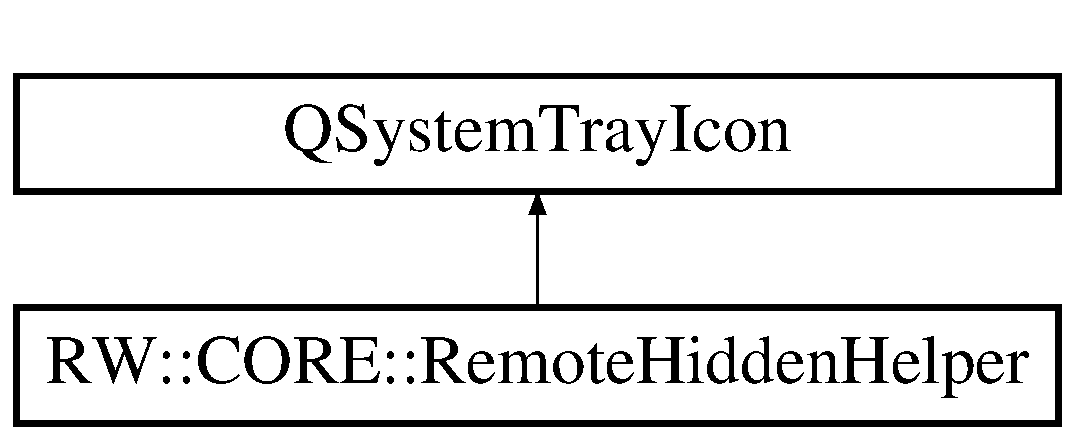
\includegraphics[height=2.000000cm]{class_r_w_1_1_c_o_r_e_1_1_remote_hidden_helper}
\end{center}
\end{figure}
\subsection*{Public Member Functions}
\begin{DoxyCompactItemize}
\item 
\hyperlink{class_r_w_1_1_c_o_r_e_1_1_remote_hidden_helper_a605994a170cd9a99b270159662d14d97}{Remote\+Hidden\+Helper} (Q\+Object $\ast$parent=0)
\item 
\hyperlink{class_r_w_1_1_c_o_r_e_1_1_remote_hidden_helper_ac7e3c2bbb6a671aa2cd5cfb39b70f28e}{$\sim$\+Remote\+Hidden\+Helper} ()
\end{DoxyCompactItemize}
\subsection*{Private Attributes}
\begin{DoxyCompactItemize}
\item 
\hyperlink{class_r_w_1_1_c_o_r_e_1_1_process_manager}{Process\+Manager} $\ast$ \hyperlink{class_r_w_1_1_c_o_r_e_1_1_remote_hidden_helper_af8e698e8aaf6a6ff89f03691494c3165}{m\+\_\+\+Process\+Manager}
\end{DoxyCompactItemize}


\subsection{Detailed Description}


Definition at line 10 of file remotehiddenhelper.\+h.



\subsection{Constructor \& Destructor Documentation}
\hypertarget{class_r_w_1_1_c_o_r_e_1_1_remote_hidden_helper_a605994a170cd9a99b270159662d14d97}{}\label{class_r_w_1_1_c_o_r_e_1_1_remote_hidden_helper_a605994a170cd9a99b270159662d14d97} 
\index{R\+W\+::\+C\+O\+R\+E\+::\+Remote\+Hidden\+Helper@{R\+W\+::\+C\+O\+R\+E\+::\+Remote\+Hidden\+Helper}!Remote\+Hidden\+Helper@{Remote\+Hidden\+Helper}}
\index{Remote\+Hidden\+Helper@{Remote\+Hidden\+Helper}!R\+W\+::\+C\+O\+R\+E\+::\+Remote\+Hidden\+Helper@{R\+W\+::\+C\+O\+R\+E\+::\+Remote\+Hidden\+Helper}}
\subsubsection{\texorpdfstring{Remote\+Hidden\+Helper()}{RemoteHiddenHelper()}}
{\footnotesize\ttfamily R\+W\+::\+C\+O\+R\+E\+::\+Remote\+Hidden\+Helper\+::\+Remote\+Hidden\+Helper (\begin{DoxyParamCaption}\item[{Q\+Object $\ast$}]{parent = {\ttfamily 0} }\end{DoxyParamCaption})}



Definition at line 9 of file remotehiddenhelper.\+cpp.

\hypertarget{class_r_w_1_1_c_o_r_e_1_1_remote_hidden_helper_ac7e3c2bbb6a671aa2cd5cfb39b70f28e}{}\label{class_r_w_1_1_c_o_r_e_1_1_remote_hidden_helper_ac7e3c2bbb6a671aa2cd5cfb39b70f28e} 
\index{R\+W\+::\+C\+O\+R\+E\+::\+Remote\+Hidden\+Helper@{R\+W\+::\+C\+O\+R\+E\+::\+Remote\+Hidden\+Helper}!````~Remote\+Hidden\+Helper@{$\sim$\+Remote\+Hidden\+Helper}}
\index{````~Remote\+Hidden\+Helper@{$\sim$\+Remote\+Hidden\+Helper}!R\+W\+::\+C\+O\+R\+E\+::\+Remote\+Hidden\+Helper@{R\+W\+::\+C\+O\+R\+E\+::\+Remote\+Hidden\+Helper}}
\subsubsection{\texorpdfstring{$\sim$\+Remote\+Hidden\+Helper()}{~RemoteHiddenHelper()}}
{\footnotesize\ttfamily R\+W\+::\+C\+O\+R\+E\+::\+Remote\+Hidden\+Helper\+::$\sim$\+Remote\+Hidden\+Helper (\begin{DoxyParamCaption}{ }\end{DoxyParamCaption})}



Definition at line 17 of file remotehiddenhelper.\+cpp.



\subsection{Member Data Documentation}
\hypertarget{class_r_w_1_1_c_o_r_e_1_1_remote_hidden_helper_af8e698e8aaf6a6ff89f03691494c3165}{}\label{class_r_w_1_1_c_o_r_e_1_1_remote_hidden_helper_af8e698e8aaf6a6ff89f03691494c3165} 
\index{R\+W\+::\+C\+O\+R\+E\+::\+Remote\+Hidden\+Helper@{R\+W\+::\+C\+O\+R\+E\+::\+Remote\+Hidden\+Helper}!m\+\_\+\+Process\+Manager@{m\+\_\+\+Process\+Manager}}
\index{m\+\_\+\+Process\+Manager@{m\+\_\+\+Process\+Manager}!R\+W\+::\+C\+O\+R\+E\+::\+Remote\+Hidden\+Helper@{R\+W\+::\+C\+O\+R\+E\+::\+Remote\+Hidden\+Helper}}
\subsubsection{\texorpdfstring{m\+\_\+\+Process\+Manager}{m\_ProcessManager}}
{\footnotesize\ttfamily \hyperlink{class_r_w_1_1_c_o_r_e_1_1_process_manager}{Process\+Manager}$\ast$ R\+W\+::\+C\+O\+R\+E\+::\+Remote\+Hidden\+Helper\+::m\+\_\+\+Process\+Manager\hspace{0.3cm}{\ttfamily [private]}}



Definition at line 15 of file remotehiddenhelper.\+h.



The documentation for this class was generated from the following files\+:\begin{DoxyCompactItemize}
\item 
C\+:/\+Projekte/\+Remote\+Repros/\+Remote\+Hidden\+Helper/\+Remote\+Hidden\+Helper/\hyperlink{remotehiddenhelper_8h}{remotehiddenhelper.\+h}\item 
C\+:/\+Projekte/\+Remote\+Repros/\+Remote\+Hidden\+Helper/\+Remote\+Hidden\+Helper/\hyperlink{remotehiddenhelper_8cpp}{remotehiddenhelper.\+cpp}\end{DoxyCompactItemize}

\hypertarget{class_ui_1_1_remote_hidden_helper_class}{}\section{Ui\+:\+:Remote\+Hidden\+Helper\+Class Class Reference}
\label{class_ui_1_1_remote_hidden_helper_class}\index{Ui\+::\+Remote\+Hidden\+Helper\+Class@{Ui\+::\+Remote\+Hidden\+Helper\+Class}}


{\ttfamily \#include $<$ui\+\_\+remotehiddenhelper.\+h$>$}

Inheritance diagram for Ui\+:\+:Remote\+Hidden\+Helper\+Class\+:\begin{figure}[H]
\begin{center}
\leavevmode
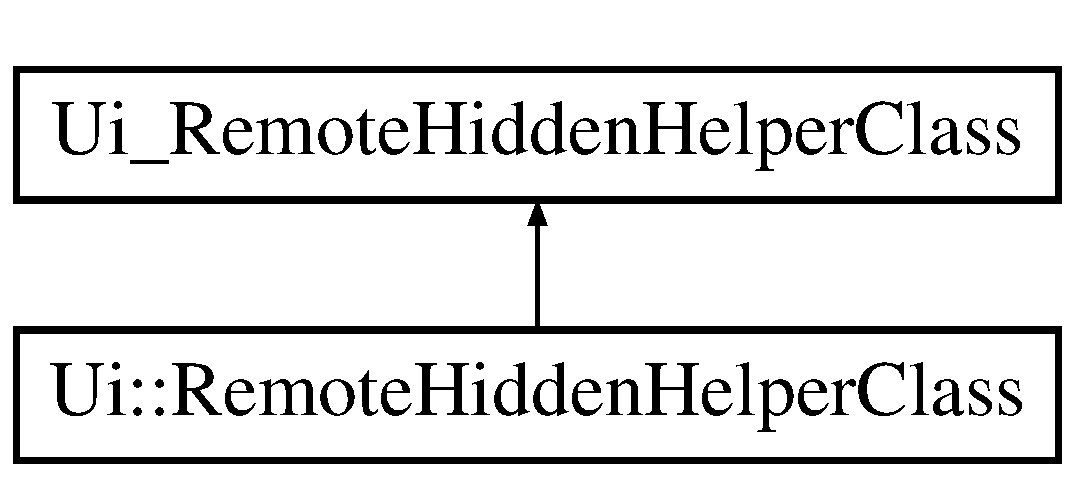
\includegraphics[height=2.000000cm]{class_ui_1_1_remote_hidden_helper_class}
\end{center}
\end{figure}
\subsection*{Additional Inherited Members}


\subsection{Detailed Description}


Definition at line 255 of file ui\+\_\+remotehiddenhelper.\+h.



The documentation for this class was generated from the following file\+:\begin{DoxyCompactItemize}
\item 
C\+:/\+Projekte/\+Remote\+Repros/\+Remote\+Hidden\+Helper/\+Remote\+Hidden\+Helper/\+Generated\+Files/\hyperlink{ui__remotehiddenhelper_8h}{ui\+\_\+remotehiddenhelper.\+h}\end{DoxyCompactItemize}

\hypertarget{class_ui___remote_hidden_helper_class}{}\section{Ui\+\_\+\+Remote\+Hidden\+Helper\+Class Class Reference}
\label{class_ui___remote_hidden_helper_class}\index{Ui\+\_\+\+Remote\+Hidden\+Helper\+Class@{Ui\+\_\+\+Remote\+Hidden\+Helper\+Class}}


{\ttfamily \#include $<$ui\+\_\+remotehiddenhelper.\+h$>$}

Inheritance diagram for Ui\+\_\+\+Remote\+Hidden\+Helper\+Class\+:\begin{figure}[H]
\begin{center}
\leavevmode
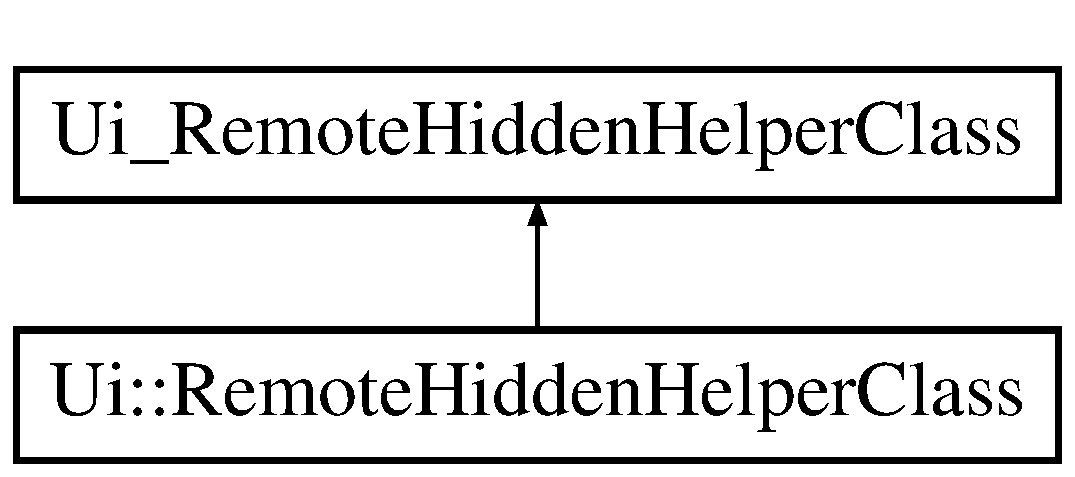
\includegraphics[height=2.000000cm]{class_ui___remote_hidden_helper_class}
\end{center}
\end{figure}
\subsection*{Public Member Functions}
\begin{DoxyCompactItemize}
\item 
void \hyperlink{class_ui___remote_hidden_helper_class_acdd6f5a5bebf921d5fcec8489a3fff1e}{setup\+Ui} (Q\+Main\+Window $\ast$Remote\+Hidden\+Helper\+Class)
\item 
void \hyperlink{class_ui___remote_hidden_helper_class_a393b3811be6e056a98239ede71c80ec9}{retranslate\+Ui} (Q\+Main\+Window $\ast$Remote\+Hidden\+Helper\+Class)
\end{DoxyCompactItemize}
\subsection*{Public Attributes}
\begin{DoxyCompactItemize}
\item 
Q\+Widget $\ast$ \hyperlink{class_ui___remote_hidden_helper_class_a28470fdc0142e3db77eecdb15fbef5af}{central\+Widget}
\item 
Q\+H\+Box\+Layout $\ast$ \hyperlink{class_ui___remote_hidden_helper_class_ad5fcb5626484231afcfe7d8d11b89a6d}{horizontal\+Layout}
\item 
Q\+V\+Box\+Layout $\ast$ \hyperlink{class_ui___remote_hidden_helper_class_af7ac92efd58256c9c12cc70d34642b73}{vertical\+Layout}
\item 
Q\+Tab\+Widget $\ast$ \hyperlink{class_ui___remote_hidden_helper_class_acf56d127ecf6c695cdbdbd5f278c1364}{tab\+Widget}
\item 
Q\+Widget $\ast$ \hyperlink{class_ui___remote_hidden_helper_class_ab2f4e6915ef33b574ce662be194b9180}{Integration}
\item 
Q\+V\+Box\+Layout $\ast$ \hyperlink{class_ui___remote_hidden_helper_class_a47a3e0139bbcce07fe9aa8260b940b3d}{vertical\+Layout\+\_\+4}
\item 
Q\+H\+Box\+Layout $\ast$ \hyperlink{class_ui___remote_hidden_helper_class_a168bb48b75379a664f73ae108a00863f}{horizontal\+Layout\+\_\+2}
\item 
Q\+V\+Box\+Layout $\ast$ \hyperlink{class_ui___remote_hidden_helper_class_aa49b047e44f29fe1c496137febfec9f2}{vertical\+Layout\+\_\+12}
\item 
Q\+Push\+Button $\ast$ \hyperlink{class_ui___remote_hidden_helper_class_ae023c25b1357ab47d7457aa6ce3ea8d5}{btn\+Flash}
\item 
Q\+Group\+Box $\ast$ \hyperlink{class_ui___remote_hidden_helper_class_a1e32f50dddf9deebdf5e9c0acc5b95eb}{group\+Box}
\item 
Q\+V\+Box\+Layout $\ast$ \hyperlink{class_ui___remote_hidden_helper_class_abd56027c9ccdaa206aacad1d7bce3eaf}{vertical\+Layout\+\_\+14}
\item 
Q\+V\+Box\+Layout $\ast$ \hyperlink{class_ui___remote_hidden_helper_class_abccfcb5d74742fed5d64978da9ebc4b8}{vertical\+Layout\+\_\+13}
\item 
Q\+Check\+Box $\ast$ \hyperlink{class_ui___remote_hidden_helper_class_a6caf14f533d691c1245bf2a152a4e742}{cbx\+Bootloader}
\item 
Q\+Check\+Box $\ast$ \hyperlink{class_ui___remote_hidden_helper_class_ad0546671fd7bf35b31518d5dcb721664}{cbx\+AC}
\item 
Q\+Check\+Box $\ast$ \hyperlink{class_ui___remote_hidden_helper_class_a51b54c903e7919f1b6518d013116e58e}{cbx\+GC}
\item 
Q\+V\+Box\+Layout $\ast$ \hyperlink{class_ui___remote_hidden_helper_class_a1060db6b11dc90b7cd55a0171d4a1f9d}{vertical\+Layout\+\_\+11}
\item 
Q\+Label $\ast$ \hyperlink{class_ui___remote_hidden_helper_class_addc6406f18551bec62d57733aaee4a0e}{l\+Project}
\item 
Q\+Combo\+Box $\ast$ \hyperlink{class_ui___remote_hidden_helper_class_a7caecd9759e6ff52726b548279021140}{cb\+Project}
\item 
Q\+Label $\ast$ \hyperlink{class_ui___remote_hidden_helper_class_add28abff8a8f0534cdfffeb33ba4faaf}{l\+Sample\+Phase}
\item 
Q\+Combo\+Box $\ast$ \hyperlink{class_ui___remote_hidden_helper_class_ae3964614499043876a7a8bc28130fb94}{cb\+Sample\+Phase}
\item 
Q\+Label $\ast$ \hyperlink{class_ui___remote_hidden_helper_class_a2105c5fa8a1d1b475d7773791b32d856}{l\+Release}
\item 
Q\+Combo\+Box $\ast$ \hyperlink{class_ui___remote_hidden_helper_class_aa7a97b774b94a003204ab5e01dc435ae}{cb\+Release}
\item 
Q\+V\+Box\+Layout $\ast$ \hyperlink{class_ui___remote_hidden_helper_class_ad22dc7780120a5ada99015716388a2b8}{vertical\+Layout\+\_\+2}
\item 
Q\+List\+View $\ast$ \hyperlink{class_ui___remote_hidden_helper_class_a7c39b8238e6c9fc7943d801213bd76e8}{list\+View}
\item 
Q\+Widget $\ast$ \hyperlink{class_ui___remote_hidden_helper_class_ac10b9b3c90ebc8ee171f32ac9b9af200}{tab\+\_\+2}
\item 
Q\+H\+Box\+Layout $\ast$ \hyperlink{class_ui___remote_hidden_helper_class_a2f6542559743da2dda19c64adc2c9293}{horizontal\+Layout\+\_\+4}
\item 
Q\+Frame $\ast$ \hyperlink{class_ui___remote_hidden_helper_class_aff7dcaaffceec85210d256c0e1bd0e2a}{frame}
\item 
Q\+Widget $\ast$ \hyperlink{class_ui___remote_hidden_helper_class_ae37c455b5bea2ecfd49d5f4bcc42f817}{tab}
\item 
Q\+Menu\+Bar $\ast$ \hyperlink{class_ui___remote_hidden_helper_class_a5070c6224e8c4c0de41bcf625ac9abf0}{menu\+Bar}
\item 
Q\+Tool\+Bar $\ast$ \hyperlink{class_ui___remote_hidden_helper_class_a2e835959e777a658b3b38ae3848b37de}{main\+Tool\+Bar}
\item 
Q\+Status\+Bar $\ast$ \hyperlink{class_ui___remote_hidden_helper_class_aec299b00778de7ae92f885205fbd2820}{status\+Bar}
\end{DoxyCompactItemize}


\subsection{Detailed Description}


Definition at line 35 of file ui\+\_\+remotehiddenhelper.\+h.



\subsection{Member Function Documentation}
\hypertarget{class_ui___remote_hidden_helper_class_a393b3811be6e056a98239ede71c80ec9}{}\label{class_ui___remote_hidden_helper_class_a393b3811be6e056a98239ede71c80ec9} 
\index{Ui\+\_\+\+Remote\+Hidden\+Helper\+Class@{Ui\+\_\+\+Remote\+Hidden\+Helper\+Class}!retranslate\+Ui@{retranslate\+Ui}}
\index{retranslate\+Ui@{retranslate\+Ui}!Ui\+\_\+\+Remote\+Hidden\+Helper\+Class@{Ui\+\_\+\+Remote\+Hidden\+Helper\+Class}}
\subsubsection{\texorpdfstring{retranslate\+Ui()}{retranslateUi()}}
{\footnotesize\ttfamily void Ui\+\_\+\+Remote\+Hidden\+Helper\+Class\+::retranslate\+Ui (\begin{DoxyParamCaption}\item[{Q\+Main\+Window $\ast$}]{Remote\+Hidden\+Helper\+Class }\end{DoxyParamCaption})\hspace{0.3cm}{\ttfamily [inline]}}



Definition at line 236 of file ui\+\_\+remotehiddenhelper.\+h.

\hypertarget{class_ui___remote_hidden_helper_class_acdd6f5a5bebf921d5fcec8489a3fff1e}{}\label{class_ui___remote_hidden_helper_class_acdd6f5a5bebf921d5fcec8489a3fff1e} 
\index{Ui\+\_\+\+Remote\+Hidden\+Helper\+Class@{Ui\+\_\+\+Remote\+Hidden\+Helper\+Class}!setup\+Ui@{setup\+Ui}}
\index{setup\+Ui@{setup\+Ui}!Ui\+\_\+\+Remote\+Hidden\+Helper\+Class@{Ui\+\_\+\+Remote\+Hidden\+Helper\+Class}}
\subsubsection{\texorpdfstring{setup\+Ui()}{setupUi()}}
{\footnotesize\ttfamily void Ui\+\_\+\+Remote\+Hidden\+Helper\+Class\+::setup\+Ui (\begin{DoxyParamCaption}\item[{Q\+Main\+Window $\ast$}]{Remote\+Hidden\+Helper\+Class }\end{DoxyParamCaption})\hspace{0.3cm}{\ttfamily [inline]}}



Definition at line 70 of file ui\+\_\+remotehiddenhelper.\+h.



\subsection{Member Data Documentation}
\hypertarget{class_ui___remote_hidden_helper_class_ae023c25b1357ab47d7457aa6ce3ea8d5}{}\label{class_ui___remote_hidden_helper_class_ae023c25b1357ab47d7457aa6ce3ea8d5} 
\index{Ui\+\_\+\+Remote\+Hidden\+Helper\+Class@{Ui\+\_\+\+Remote\+Hidden\+Helper\+Class}!btn\+Flash@{btn\+Flash}}
\index{btn\+Flash@{btn\+Flash}!Ui\+\_\+\+Remote\+Hidden\+Helper\+Class@{Ui\+\_\+\+Remote\+Hidden\+Helper\+Class}}
\subsubsection{\texorpdfstring{btn\+Flash}{btnFlash}}
{\footnotesize\ttfamily Q\+Push\+Button$\ast$ Ui\+\_\+\+Remote\+Hidden\+Helper\+Class\+::btn\+Flash}



Definition at line 46 of file ui\+\_\+remotehiddenhelper.\+h.

\hypertarget{class_ui___remote_hidden_helper_class_a7caecd9759e6ff52726b548279021140}{}\label{class_ui___remote_hidden_helper_class_a7caecd9759e6ff52726b548279021140} 
\index{Ui\+\_\+\+Remote\+Hidden\+Helper\+Class@{Ui\+\_\+\+Remote\+Hidden\+Helper\+Class}!cb\+Project@{cb\+Project}}
\index{cb\+Project@{cb\+Project}!Ui\+\_\+\+Remote\+Hidden\+Helper\+Class@{Ui\+\_\+\+Remote\+Hidden\+Helper\+Class}}
\subsubsection{\texorpdfstring{cb\+Project}{cbProject}}
{\footnotesize\ttfamily Q\+Combo\+Box$\ast$ Ui\+\_\+\+Remote\+Hidden\+Helper\+Class\+::cb\+Project}



Definition at line 55 of file ui\+\_\+remotehiddenhelper.\+h.

\hypertarget{class_ui___remote_hidden_helper_class_aa7a97b774b94a003204ab5e01dc435ae}{}\label{class_ui___remote_hidden_helper_class_aa7a97b774b94a003204ab5e01dc435ae} 
\index{Ui\+\_\+\+Remote\+Hidden\+Helper\+Class@{Ui\+\_\+\+Remote\+Hidden\+Helper\+Class}!cb\+Release@{cb\+Release}}
\index{cb\+Release@{cb\+Release}!Ui\+\_\+\+Remote\+Hidden\+Helper\+Class@{Ui\+\_\+\+Remote\+Hidden\+Helper\+Class}}
\subsubsection{\texorpdfstring{cb\+Release}{cbRelease}}
{\footnotesize\ttfamily Q\+Combo\+Box$\ast$ Ui\+\_\+\+Remote\+Hidden\+Helper\+Class\+::cb\+Release}



Definition at line 59 of file ui\+\_\+remotehiddenhelper.\+h.

\hypertarget{class_ui___remote_hidden_helper_class_ae3964614499043876a7a8bc28130fb94}{}\label{class_ui___remote_hidden_helper_class_ae3964614499043876a7a8bc28130fb94} 
\index{Ui\+\_\+\+Remote\+Hidden\+Helper\+Class@{Ui\+\_\+\+Remote\+Hidden\+Helper\+Class}!cb\+Sample\+Phase@{cb\+Sample\+Phase}}
\index{cb\+Sample\+Phase@{cb\+Sample\+Phase}!Ui\+\_\+\+Remote\+Hidden\+Helper\+Class@{Ui\+\_\+\+Remote\+Hidden\+Helper\+Class}}
\subsubsection{\texorpdfstring{cb\+Sample\+Phase}{cbSamplePhase}}
{\footnotesize\ttfamily Q\+Combo\+Box$\ast$ Ui\+\_\+\+Remote\+Hidden\+Helper\+Class\+::cb\+Sample\+Phase}



Definition at line 57 of file ui\+\_\+remotehiddenhelper.\+h.

\hypertarget{class_ui___remote_hidden_helper_class_ad0546671fd7bf35b31518d5dcb721664}{}\label{class_ui___remote_hidden_helper_class_ad0546671fd7bf35b31518d5dcb721664} 
\index{Ui\+\_\+\+Remote\+Hidden\+Helper\+Class@{Ui\+\_\+\+Remote\+Hidden\+Helper\+Class}!cbx\+AC@{cbx\+AC}}
\index{cbx\+AC@{cbx\+AC}!Ui\+\_\+\+Remote\+Hidden\+Helper\+Class@{Ui\+\_\+\+Remote\+Hidden\+Helper\+Class}}
\subsubsection{\texorpdfstring{cbx\+AC}{cbxAC}}
{\footnotesize\ttfamily Q\+Check\+Box$\ast$ Ui\+\_\+\+Remote\+Hidden\+Helper\+Class\+::cbx\+AC}



Definition at line 51 of file ui\+\_\+remotehiddenhelper.\+h.

\hypertarget{class_ui___remote_hidden_helper_class_a6caf14f533d691c1245bf2a152a4e742}{}\label{class_ui___remote_hidden_helper_class_a6caf14f533d691c1245bf2a152a4e742} 
\index{Ui\+\_\+\+Remote\+Hidden\+Helper\+Class@{Ui\+\_\+\+Remote\+Hidden\+Helper\+Class}!cbx\+Bootloader@{cbx\+Bootloader}}
\index{cbx\+Bootloader@{cbx\+Bootloader}!Ui\+\_\+\+Remote\+Hidden\+Helper\+Class@{Ui\+\_\+\+Remote\+Hidden\+Helper\+Class}}
\subsubsection{\texorpdfstring{cbx\+Bootloader}{cbxBootloader}}
{\footnotesize\ttfamily Q\+Check\+Box$\ast$ Ui\+\_\+\+Remote\+Hidden\+Helper\+Class\+::cbx\+Bootloader}



Definition at line 50 of file ui\+\_\+remotehiddenhelper.\+h.

\hypertarget{class_ui___remote_hidden_helper_class_a51b54c903e7919f1b6518d013116e58e}{}\label{class_ui___remote_hidden_helper_class_a51b54c903e7919f1b6518d013116e58e} 
\index{Ui\+\_\+\+Remote\+Hidden\+Helper\+Class@{Ui\+\_\+\+Remote\+Hidden\+Helper\+Class}!cbx\+GC@{cbx\+GC}}
\index{cbx\+GC@{cbx\+GC}!Ui\+\_\+\+Remote\+Hidden\+Helper\+Class@{Ui\+\_\+\+Remote\+Hidden\+Helper\+Class}}
\subsubsection{\texorpdfstring{cbx\+GC}{cbxGC}}
{\footnotesize\ttfamily Q\+Check\+Box$\ast$ Ui\+\_\+\+Remote\+Hidden\+Helper\+Class\+::cbx\+GC}



Definition at line 52 of file ui\+\_\+remotehiddenhelper.\+h.

\hypertarget{class_ui___remote_hidden_helper_class_a28470fdc0142e3db77eecdb15fbef5af}{}\label{class_ui___remote_hidden_helper_class_a28470fdc0142e3db77eecdb15fbef5af} 
\index{Ui\+\_\+\+Remote\+Hidden\+Helper\+Class@{Ui\+\_\+\+Remote\+Hidden\+Helper\+Class}!central\+Widget@{central\+Widget}}
\index{central\+Widget@{central\+Widget}!Ui\+\_\+\+Remote\+Hidden\+Helper\+Class@{Ui\+\_\+\+Remote\+Hidden\+Helper\+Class}}
\subsubsection{\texorpdfstring{central\+Widget}{centralWidget}}
{\footnotesize\ttfamily Q\+Widget$\ast$ Ui\+\_\+\+Remote\+Hidden\+Helper\+Class\+::central\+Widget}



Definition at line 38 of file ui\+\_\+remotehiddenhelper.\+h.

\hypertarget{class_ui___remote_hidden_helper_class_aff7dcaaffceec85210d256c0e1bd0e2a}{}\label{class_ui___remote_hidden_helper_class_aff7dcaaffceec85210d256c0e1bd0e2a} 
\index{Ui\+\_\+\+Remote\+Hidden\+Helper\+Class@{Ui\+\_\+\+Remote\+Hidden\+Helper\+Class}!frame@{frame}}
\index{frame@{frame}!Ui\+\_\+\+Remote\+Hidden\+Helper\+Class@{Ui\+\_\+\+Remote\+Hidden\+Helper\+Class}}
\subsubsection{\texorpdfstring{frame}{frame}}
{\footnotesize\ttfamily Q\+Frame$\ast$ Ui\+\_\+\+Remote\+Hidden\+Helper\+Class\+::frame}



Definition at line 64 of file ui\+\_\+remotehiddenhelper.\+h.

\hypertarget{class_ui___remote_hidden_helper_class_a1e32f50dddf9deebdf5e9c0acc5b95eb}{}\label{class_ui___remote_hidden_helper_class_a1e32f50dddf9deebdf5e9c0acc5b95eb} 
\index{Ui\+\_\+\+Remote\+Hidden\+Helper\+Class@{Ui\+\_\+\+Remote\+Hidden\+Helper\+Class}!group\+Box@{group\+Box}}
\index{group\+Box@{group\+Box}!Ui\+\_\+\+Remote\+Hidden\+Helper\+Class@{Ui\+\_\+\+Remote\+Hidden\+Helper\+Class}}
\subsubsection{\texorpdfstring{group\+Box}{groupBox}}
{\footnotesize\ttfamily Q\+Group\+Box$\ast$ Ui\+\_\+\+Remote\+Hidden\+Helper\+Class\+::group\+Box}



Definition at line 47 of file ui\+\_\+remotehiddenhelper.\+h.

\hypertarget{class_ui___remote_hidden_helper_class_ad5fcb5626484231afcfe7d8d11b89a6d}{}\label{class_ui___remote_hidden_helper_class_ad5fcb5626484231afcfe7d8d11b89a6d} 
\index{Ui\+\_\+\+Remote\+Hidden\+Helper\+Class@{Ui\+\_\+\+Remote\+Hidden\+Helper\+Class}!horizontal\+Layout@{horizontal\+Layout}}
\index{horizontal\+Layout@{horizontal\+Layout}!Ui\+\_\+\+Remote\+Hidden\+Helper\+Class@{Ui\+\_\+\+Remote\+Hidden\+Helper\+Class}}
\subsubsection{\texorpdfstring{horizontal\+Layout}{horizontalLayout}}
{\footnotesize\ttfamily Q\+H\+Box\+Layout$\ast$ Ui\+\_\+\+Remote\+Hidden\+Helper\+Class\+::horizontal\+Layout}



Definition at line 39 of file ui\+\_\+remotehiddenhelper.\+h.

\hypertarget{class_ui___remote_hidden_helper_class_a168bb48b75379a664f73ae108a00863f}{}\label{class_ui___remote_hidden_helper_class_a168bb48b75379a664f73ae108a00863f} 
\index{Ui\+\_\+\+Remote\+Hidden\+Helper\+Class@{Ui\+\_\+\+Remote\+Hidden\+Helper\+Class}!horizontal\+Layout\+\_\+2@{horizontal\+Layout\+\_\+2}}
\index{horizontal\+Layout\+\_\+2@{horizontal\+Layout\+\_\+2}!Ui\+\_\+\+Remote\+Hidden\+Helper\+Class@{Ui\+\_\+\+Remote\+Hidden\+Helper\+Class}}
\subsubsection{\texorpdfstring{horizontal\+Layout\+\_\+2}{horizontalLayout\_2}}
{\footnotesize\ttfamily Q\+H\+Box\+Layout$\ast$ Ui\+\_\+\+Remote\+Hidden\+Helper\+Class\+::horizontal\+Layout\+\_\+2}



Definition at line 44 of file ui\+\_\+remotehiddenhelper.\+h.

\hypertarget{class_ui___remote_hidden_helper_class_a2f6542559743da2dda19c64adc2c9293}{}\label{class_ui___remote_hidden_helper_class_a2f6542559743da2dda19c64adc2c9293} 
\index{Ui\+\_\+\+Remote\+Hidden\+Helper\+Class@{Ui\+\_\+\+Remote\+Hidden\+Helper\+Class}!horizontal\+Layout\+\_\+4@{horizontal\+Layout\+\_\+4}}
\index{horizontal\+Layout\+\_\+4@{horizontal\+Layout\+\_\+4}!Ui\+\_\+\+Remote\+Hidden\+Helper\+Class@{Ui\+\_\+\+Remote\+Hidden\+Helper\+Class}}
\subsubsection{\texorpdfstring{horizontal\+Layout\+\_\+4}{horizontalLayout\_4}}
{\footnotesize\ttfamily Q\+H\+Box\+Layout$\ast$ Ui\+\_\+\+Remote\+Hidden\+Helper\+Class\+::horizontal\+Layout\+\_\+4}



Definition at line 63 of file ui\+\_\+remotehiddenhelper.\+h.

\hypertarget{class_ui___remote_hidden_helper_class_ab2f4e6915ef33b574ce662be194b9180}{}\label{class_ui___remote_hidden_helper_class_ab2f4e6915ef33b574ce662be194b9180} 
\index{Ui\+\_\+\+Remote\+Hidden\+Helper\+Class@{Ui\+\_\+\+Remote\+Hidden\+Helper\+Class}!Integration@{Integration}}
\index{Integration@{Integration}!Ui\+\_\+\+Remote\+Hidden\+Helper\+Class@{Ui\+\_\+\+Remote\+Hidden\+Helper\+Class}}
\subsubsection{\texorpdfstring{Integration}{Integration}}
{\footnotesize\ttfamily Q\+Widget$\ast$ Ui\+\_\+\+Remote\+Hidden\+Helper\+Class\+::\+Integration}



Definition at line 42 of file ui\+\_\+remotehiddenhelper.\+h.

\hypertarget{class_ui___remote_hidden_helper_class_a7c39b8238e6c9fc7943d801213bd76e8}{}\label{class_ui___remote_hidden_helper_class_a7c39b8238e6c9fc7943d801213bd76e8} 
\index{Ui\+\_\+\+Remote\+Hidden\+Helper\+Class@{Ui\+\_\+\+Remote\+Hidden\+Helper\+Class}!list\+View@{list\+View}}
\index{list\+View@{list\+View}!Ui\+\_\+\+Remote\+Hidden\+Helper\+Class@{Ui\+\_\+\+Remote\+Hidden\+Helper\+Class}}
\subsubsection{\texorpdfstring{list\+View}{listView}}
{\footnotesize\ttfamily Q\+List\+View$\ast$ Ui\+\_\+\+Remote\+Hidden\+Helper\+Class\+::list\+View}



Definition at line 61 of file ui\+\_\+remotehiddenhelper.\+h.

\hypertarget{class_ui___remote_hidden_helper_class_addc6406f18551bec62d57733aaee4a0e}{}\label{class_ui___remote_hidden_helper_class_addc6406f18551bec62d57733aaee4a0e} 
\index{Ui\+\_\+\+Remote\+Hidden\+Helper\+Class@{Ui\+\_\+\+Remote\+Hidden\+Helper\+Class}!l\+Project@{l\+Project}}
\index{l\+Project@{l\+Project}!Ui\+\_\+\+Remote\+Hidden\+Helper\+Class@{Ui\+\_\+\+Remote\+Hidden\+Helper\+Class}}
\subsubsection{\texorpdfstring{l\+Project}{lProject}}
{\footnotesize\ttfamily Q\+Label$\ast$ Ui\+\_\+\+Remote\+Hidden\+Helper\+Class\+::l\+Project}



Definition at line 54 of file ui\+\_\+remotehiddenhelper.\+h.

\hypertarget{class_ui___remote_hidden_helper_class_a2105c5fa8a1d1b475d7773791b32d856}{}\label{class_ui___remote_hidden_helper_class_a2105c5fa8a1d1b475d7773791b32d856} 
\index{Ui\+\_\+\+Remote\+Hidden\+Helper\+Class@{Ui\+\_\+\+Remote\+Hidden\+Helper\+Class}!l\+Release@{l\+Release}}
\index{l\+Release@{l\+Release}!Ui\+\_\+\+Remote\+Hidden\+Helper\+Class@{Ui\+\_\+\+Remote\+Hidden\+Helper\+Class}}
\subsubsection{\texorpdfstring{l\+Release}{lRelease}}
{\footnotesize\ttfamily Q\+Label$\ast$ Ui\+\_\+\+Remote\+Hidden\+Helper\+Class\+::l\+Release}



Definition at line 58 of file ui\+\_\+remotehiddenhelper.\+h.

\hypertarget{class_ui___remote_hidden_helper_class_add28abff8a8f0534cdfffeb33ba4faaf}{}\label{class_ui___remote_hidden_helper_class_add28abff8a8f0534cdfffeb33ba4faaf} 
\index{Ui\+\_\+\+Remote\+Hidden\+Helper\+Class@{Ui\+\_\+\+Remote\+Hidden\+Helper\+Class}!l\+Sample\+Phase@{l\+Sample\+Phase}}
\index{l\+Sample\+Phase@{l\+Sample\+Phase}!Ui\+\_\+\+Remote\+Hidden\+Helper\+Class@{Ui\+\_\+\+Remote\+Hidden\+Helper\+Class}}
\subsubsection{\texorpdfstring{l\+Sample\+Phase}{lSamplePhase}}
{\footnotesize\ttfamily Q\+Label$\ast$ Ui\+\_\+\+Remote\+Hidden\+Helper\+Class\+::l\+Sample\+Phase}



Definition at line 56 of file ui\+\_\+remotehiddenhelper.\+h.

\hypertarget{class_ui___remote_hidden_helper_class_a2e835959e777a658b3b38ae3848b37de}{}\label{class_ui___remote_hidden_helper_class_a2e835959e777a658b3b38ae3848b37de} 
\index{Ui\+\_\+\+Remote\+Hidden\+Helper\+Class@{Ui\+\_\+\+Remote\+Hidden\+Helper\+Class}!main\+Tool\+Bar@{main\+Tool\+Bar}}
\index{main\+Tool\+Bar@{main\+Tool\+Bar}!Ui\+\_\+\+Remote\+Hidden\+Helper\+Class@{Ui\+\_\+\+Remote\+Hidden\+Helper\+Class}}
\subsubsection{\texorpdfstring{main\+Tool\+Bar}{mainToolBar}}
{\footnotesize\ttfamily Q\+Tool\+Bar$\ast$ Ui\+\_\+\+Remote\+Hidden\+Helper\+Class\+::main\+Tool\+Bar}



Definition at line 67 of file ui\+\_\+remotehiddenhelper.\+h.

\hypertarget{class_ui___remote_hidden_helper_class_a5070c6224e8c4c0de41bcf625ac9abf0}{}\label{class_ui___remote_hidden_helper_class_a5070c6224e8c4c0de41bcf625ac9abf0} 
\index{Ui\+\_\+\+Remote\+Hidden\+Helper\+Class@{Ui\+\_\+\+Remote\+Hidden\+Helper\+Class}!menu\+Bar@{menu\+Bar}}
\index{menu\+Bar@{menu\+Bar}!Ui\+\_\+\+Remote\+Hidden\+Helper\+Class@{Ui\+\_\+\+Remote\+Hidden\+Helper\+Class}}
\subsubsection{\texorpdfstring{menu\+Bar}{menuBar}}
{\footnotesize\ttfamily Q\+Menu\+Bar$\ast$ Ui\+\_\+\+Remote\+Hidden\+Helper\+Class\+::menu\+Bar}



Definition at line 66 of file ui\+\_\+remotehiddenhelper.\+h.

\hypertarget{class_ui___remote_hidden_helper_class_aec299b00778de7ae92f885205fbd2820}{}\label{class_ui___remote_hidden_helper_class_aec299b00778de7ae92f885205fbd2820} 
\index{Ui\+\_\+\+Remote\+Hidden\+Helper\+Class@{Ui\+\_\+\+Remote\+Hidden\+Helper\+Class}!status\+Bar@{status\+Bar}}
\index{status\+Bar@{status\+Bar}!Ui\+\_\+\+Remote\+Hidden\+Helper\+Class@{Ui\+\_\+\+Remote\+Hidden\+Helper\+Class}}
\subsubsection{\texorpdfstring{status\+Bar}{statusBar}}
{\footnotesize\ttfamily Q\+Status\+Bar$\ast$ Ui\+\_\+\+Remote\+Hidden\+Helper\+Class\+::status\+Bar}



Definition at line 68 of file ui\+\_\+remotehiddenhelper.\+h.

\hypertarget{class_ui___remote_hidden_helper_class_ae37c455b5bea2ecfd49d5f4bcc42f817}{}\label{class_ui___remote_hidden_helper_class_ae37c455b5bea2ecfd49d5f4bcc42f817} 
\index{Ui\+\_\+\+Remote\+Hidden\+Helper\+Class@{Ui\+\_\+\+Remote\+Hidden\+Helper\+Class}!tab@{tab}}
\index{tab@{tab}!Ui\+\_\+\+Remote\+Hidden\+Helper\+Class@{Ui\+\_\+\+Remote\+Hidden\+Helper\+Class}}
\subsubsection{\texorpdfstring{tab}{tab}}
{\footnotesize\ttfamily Q\+Widget$\ast$ Ui\+\_\+\+Remote\+Hidden\+Helper\+Class\+::tab}



Definition at line 65 of file ui\+\_\+remotehiddenhelper.\+h.

\hypertarget{class_ui___remote_hidden_helper_class_ac10b9b3c90ebc8ee171f32ac9b9af200}{}\label{class_ui___remote_hidden_helper_class_ac10b9b3c90ebc8ee171f32ac9b9af200} 
\index{Ui\+\_\+\+Remote\+Hidden\+Helper\+Class@{Ui\+\_\+\+Remote\+Hidden\+Helper\+Class}!tab\+\_\+2@{tab\+\_\+2}}
\index{tab\+\_\+2@{tab\+\_\+2}!Ui\+\_\+\+Remote\+Hidden\+Helper\+Class@{Ui\+\_\+\+Remote\+Hidden\+Helper\+Class}}
\subsubsection{\texorpdfstring{tab\+\_\+2}{tab\_2}}
{\footnotesize\ttfamily Q\+Widget$\ast$ Ui\+\_\+\+Remote\+Hidden\+Helper\+Class\+::tab\+\_\+2}



Definition at line 62 of file ui\+\_\+remotehiddenhelper.\+h.

\hypertarget{class_ui___remote_hidden_helper_class_acf56d127ecf6c695cdbdbd5f278c1364}{}\label{class_ui___remote_hidden_helper_class_acf56d127ecf6c695cdbdbd5f278c1364} 
\index{Ui\+\_\+\+Remote\+Hidden\+Helper\+Class@{Ui\+\_\+\+Remote\+Hidden\+Helper\+Class}!tab\+Widget@{tab\+Widget}}
\index{tab\+Widget@{tab\+Widget}!Ui\+\_\+\+Remote\+Hidden\+Helper\+Class@{Ui\+\_\+\+Remote\+Hidden\+Helper\+Class}}
\subsubsection{\texorpdfstring{tab\+Widget}{tabWidget}}
{\footnotesize\ttfamily Q\+Tab\+Widget$\ast$ Ui\+\_\+\+Remote\+Hidden\+Helper\+Class\+::tab\+Widget}



Definition at line 41 of file ui\+\_\+remotehiddenhelper.\+h.

\hypertarget{class_ui___remote_hidden_helper_class_af7ac92efd58256c9c12cc70d34642b73}{}\label{class_ui___remote_hidden_helper_class_af7ac92efd58256c9c12cc70d34642b73} 
\index{Ui\+\_\+\+Remote\+Hidden\+Helper\+Class@{Ui\+\_\+\+Remote\+Hidden\+Helper\+Class}!vertical\+Layout@{vertical\+Layout}}
\index{vertical\+Layout@{vertical\+Layout}!Ui\+\_\+\+Remote\+Hidden\+Helper\+Class@{Ui\+\_\+\+Remote\+Hidden\+Helper\+Class}}
\subsubsection{\texorpdfstring{vertical\+Layout}{verticalLayout}}
{\footnotesize\ttfamily Q\+V\+Box\+Layout$\ast$ Ui\+\_\+\+Remote\+Hidden\+Helper\+Class\+::vertical\+Layout}



Definition at line 40 of file ui\+\_\+remotehiddenhelper.\+h.

\hypertarget{class_ui___remote_hidden_helper_class_a1060db6b11dc90b7cd55a0171d4a1f9d}{}\label{class_ui___remote_hidden_helper_class_a1060db6b11dc90b7cd55a0171d4a1f9d} 
\index{Ui\+\_\+\+Remote\+Hidden\+Helper\+Class@{Ui\+\_\+\+Remote\+Hidden\+Helper\+Class}!vertical\+Layout\+\_\+11@{vertical\+Layout\+\_\+11}}
\index{vertical\+Layout\+\_\+11@{vertical\+Layout\+\_\+11}!Ui\+\_\+\+Remote\+Hidden\+Helper\+Class@{Ui\+\_\+\+Remote\+Hidden\+Helper\+Class}}
\subsubsection{\texorpdfstring{vertical\+Layout\+\_\+11}{verticalLayout\_11}}
{\footnotesize\ttfamily Q\+V\+Box\+Layout$\ast$ Ui\+\_\+\+Remote\+Hidden\+Helper\+Class\+::vertical\+Layout\+\_\+11}



Definition at line 53 of file ui\+\_\+remotehiddenhelper.\+h.

\hypertarget{class_ui___remote_hidden_helper_class_aa49b047e44f29fe1c496137febfec9f2}{}\label{class_ui___remote_hidden_helper_class_aa49b047e44f29fe1c496137febfec9f2} 
\index{Ui\+\_\+\+Remote\+Hidden\+Helper\+Class@{Ui\+\_\+\+Remote\+Hidden\+Helper\+Class}!vertical\+Layout\+\_\+12@{vertical\+Layout\+\_\+12}}
\index{vertical\+Layout\+\_\+12@{vertical\+Layout\+\_\+12}!Ui\+\_\+\+Remote\+Hidden\+Helper\+Class@{Ui\+\_\+\+Remote\+Hidden\+Helper\+Class}}
\subsubsection{\texorpdfstring{vertical\+Layout\+\_\+12}{verticalLayout\_12}}
{\footnotesize\ttfamily Q\+V\+Box\+Layout$\ast$ Ui\+\_\+\+Remote\+Hidden\+Helper\+Class\+::vertical\+Layout\+\_\+12}



Definition at line 45 of file ui\+\_\+remotehiddenhelper.\+h.

\hypertarget{class_ui___remote_hidden_helper_class_abccfcb5d74742fed5d64978da9ebc4b8}{}\label{class_ui___remote_hidden_helper_class_abccfcb5d74742fed5d64978da9ebc4b8} 
\index{Ui\+\_\+\+Remote\+Hidden\+Helper\+Class@{Ui\+\_\+\+Remote\+Hidden\+Helper\+Class}!vertical\+Layout\+\_\+13@{vertical\+Layout\+\_\+13}}
\index{vertical\+Layout\+\_\+13@{vertical\+Layout\+\_\+13}!Ui\+\_\+\+Remote\+Hidden\+Helper\+Class@{Ui\+\_\+\+Remote\+Hidden\+Helper\+Class}}
\subsubsection{\texorpdfstring{vertical\+Layout\+\_\+13}{verticalLayout\_13}}
{\footnotesize\ttfamily Q\+V\+Box\+Layout$\ast$ Ui\+\_\+\+Remote\+Hidden\+Helper\+Class\+::vertical\+Layout\+\_\+13}



Definition at line 49 of file ui\+\_\+remotehiddenhelper.\+h.

\hypertarget{class_ui___remote_hidden_helper_class_abd56027c9ccdaa206aacad1d7bce3eaf}{}\label{class_ui___remote_hidden_helper_class_abd56027c9ccdaa206aacad1d7bce3eaf} 
\index{Ui\+\_\+\+Remote\+Hidden\+Helper\+Class@{Ui\+\_\+\+Remote\+Hidden\+Helper\+Class}!vertical\+Layout\+\_\+14@{vertical\+Layout\+\_\+14}}
\index{vertical\+Layout\+\_\+14@{vertical\+Layout\+\_\+14}!Ui\+\_\+\+Remote\+Hidden\+Helper\+Class@{Ui\+\_\+\+Remote\+Hidden\+Helper\+Class}}
\subsubsection{\texorpdfstring{vertical\+Layout\+\_\+14}{verticalLayout\_14}}
{\footnotesize\ttfamily Q\+V\+Box\+Layout$\ast$ Ui\+\_\+\+Remote\+Hidden\+Helper\+Class\+::vertical\+Layout\+\_\+14}



Definition at line 48 of file ui\+\_\+remotehiddenhelper.\+h.

\hypertarget{class_ui___remote_hidden_helper_class_ad22dc7780120a5ada99015716388a2b8}{}\label{class_ui___remote_hidden_helper_class_ad22dc7780120a5ada99015716388a2b8} 
\index{Ui\+\_\+\+Remote\+Hidden\+Helper\+Class@{Ui\+\_\+\+Remote\+Hidden\+Helper\+Class}!vertical\+Layout\+\_\+2@{vertical\+Layout\+\_\+2}}
\index{vertical\+Layout\+\_\+2@{vertical\+Layout\+\_\+2}!Ui\+\_\+\+Remote\+Hidden\+Helper\+Class@{Ui\+\_\+\+Remote\+Hidden\+Helper\+Class}}
\subsubsection{\texorpdfstring{vertical\+Layout\+\_\+2}{verticalLayout\_2}}
{\footnotesize\ttfamily Q\+V\+Box\+Layout$\ast$ Ui\+\_\+\+Remote\+Hidden\+Helper\+Class\+::vertical\+Layout\+\_\+2}



Definition at line 60 of file ui\+\_\+remotehiddenhelper.\+h.

\hypertarget{class_ui___remote_hidden_helper_class_a47a3e0139bbcce07fe9aa8260b940b3d}{}\label{class_ui___remote_hidden_helper_class_a47a3e0139bbcce07fe9aa8260b940b3d} 
\index{Ui\+\_\+\+Remote\+Hidden\+Helper\+Class@{Ui\+\_\+\+Remote\+Hidden\+Helper\+Class}!vertical\+Layout\+\_\+4@{vertical\+Layout\+\_\+4}}
\index{vertical\+Layout\+\_\+4@{vertical\+Layout\+\_\+4}!Ui\+\_\+\+Remote\+Hidden\+Helper\+Class@{Ui\+\_\+\+Remote\+Hidden\+Helper\+Class}}
\subsubsection{\texorpdfstring{vertical\+Layout\+\_\+4}{verticalLayout\_4}}
{\footnotesize\ttfamily Q\+V\+Box\+Layout$\ast$ Ui\+\_\+\+Remote\+Hidden\+Helper\+Class\+::vertical\+Layout\+\_\+4}



Definition at line 43 of file ui\+\_\+remotehiddenhelper.\+h.



The documentation for this class was generated from the following file\+:\begin{DoxyCompactItemize}
\item 
C\+:/\+Projekte/\+Remote\+Repros/\+Remote\+Hidden\+Helper/\+Remote\+Hidden\+Helper/\+Generated\+Files/\hyperlink{ui__remotehiddenhelper_8h}{ui\+\_\+remotehiddenhelper.\+h}\end{DoxyCompactItemize}

\hypertarget{class_r_w_1_1_c_o_r_e_1_1_unit}{}\section{RW\+:\+:C\+O\+RE\+:\+:Unit Class Reference}
\label{class_r_w_1_1_c_o_r_e_1_1_unit}\index{R\+W\+::\+C\+O\+R\+E\+::\+Unit@{R\+W\+::\+C\+O\+R\+E\+::\+Unit}}


{\ttfamily \#include $<$Unit.\+h$>$}

Inheritance diagram for RW\+:\+:C\+O\+RE\+:\+:Unit\+:\begin{figure}[H]
\begin{center}
\leavevmode
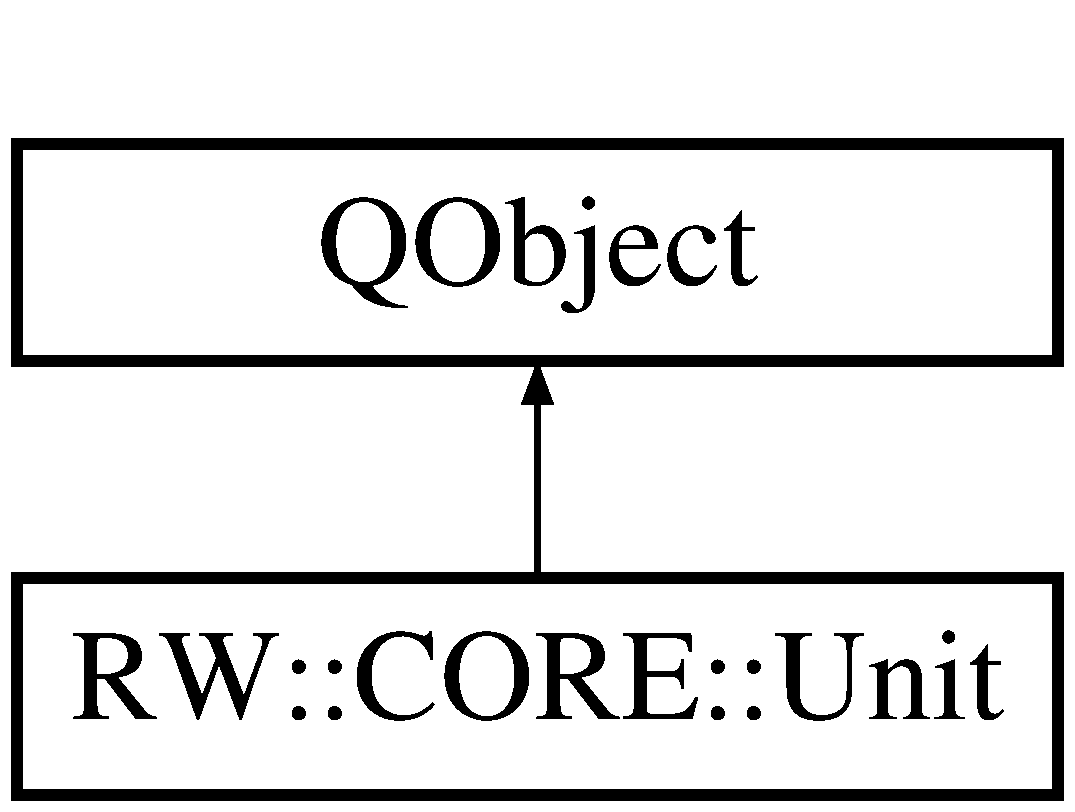
\includegraphics[height=2.000000cm]{class_r_w_1_1_c_o_r_e_1_1_unit}
\end{center}
\end{figure}
\subsection*{Public Slots}
\begin{DoxyCompactItemize}
\item 
void \hyperlink{class_r_w_1_1_c_o_r_e_1_1_unit_ac614ffc786f0c88a3397563414f8914a}{On\+Process\+Message} ()
\end{DoxyCompactItemize}
\subsection*{Public Member Functions}
\begin{DoxyCompactItemize}
\item 
\hyperlink{class_r_w_1_1_c_o_r_e_1_1_unit_a28b0dc765cd31094c074dbad370055bb}{Unit} (Q\+Local\+Socket $\ast$Socket)
\item 
\hyperlink{class_r_w_1_1_c_o_r_e_1_1_unit_ae898e2ef0f245ceb1cae8cae17b8a6f9}{$\sim$\+Unit} ()
\item 
void \hyperlink{class_r_w_1_1_c_o_r_e_1_1_unit_af2a571d5629b2742b603ab88f6c2485c}{Start\+Test} (Util\+::\+Functions Start\+Point)
\end{DoxyCompactItemize}
\subsection*{Private Member Functions}
\begin{DoxyCompactItemize}
\item 
Q\+Byte\+Array \hyperlink{class_r_w_1_1_c_o_r_e_1_1_unit_af72c1a6126550786eac95439262b9718}{Create\+Message} (Util\+::\+Functions Func, Q\+Byte\+Array \hyperlink{namespace_r_w_1_1_c_o_r_e_a571834b44d0e3fab58aa6abfe5a02988}{Message}, Util\+::\+Error\+ID Id)
\item 
void \hyperlink{class_r_w_1_1_c_o_r_e_1_1_unit_afe8b61eae2147c5ed409f16f801947a8}{Print\+Debug\+Informations} (\hyperlink{namespace_r_w_1_1_c_o_r_e_a571834b44d0e3fab58aa6abfe5a02988}{Message} \hyperlink{namespace_r_w_1_1_c_o_r_e_a571834b44d0e3fab58aa6abfe5a02988}{Message})
\item 
\hyperlink{namespace_r_w_1_1_c_o_r_e_a571834b44d0e3fab58aa6abfe5a02988}{Message} \hyperlink{class_r_w_1_1_c_o_r_e_1_1_unit_a0bd62b49be93e3e162ba08ac1c02c027}{Get\+Message} ()
\item 
void \hyperlink{class_r_w_1_1_c_o_r_e_1_1_unit_a5d5854e3dde478770720f302289dbddd}{Send\+Message} (Q\+Byte\+Array \hyperlink{namespace_r_w_1_1_c_o_r_e_a571834b44d0e3fab58aa6abfe5a02988}{Message})
\end{DoxyCompactItemize}
\subsection*{Private Attributes}
\begin{DoxyCompactItemize}
\item 
Q\+Local\+Socket $\ast$ \hyperlink{class_r_w_1_1_c_o_r_e_1_1_unit_a66126526b69f4c9f9559613e921bf724}{m\+\_\+\+Socket}
\item 
Q\+String\+List \hyperlink{class_r_w_1_1_c_o_r_e_1_1_unit_a7e19e658c1f9cac1db592ac5d29151a2}{m\+\_\+\+Flash\+Files}
\end{DoxyCompactItemize}


\subsection{Detailed Description}


Definition at line 13 of file Unit.\+h.



\subsection{Constructor \& Destructor Documentation}
\hypertarget{class_r_w_1_1_c_o_r_e_1_1_unit_a28b0dc765cd31094c074dbad370055bb}{}\label{class_r_w_1_1_c_o_r_e_1_1_unit_a28b0dc765cd31094c074dbad370055bb} 
\index{R\+W\+::\+C\+O\+R\+E\+::\+Unit@{R\+W\+::\+C\+O\+R\+E\+::\+Unit}!Unit@{Unit}}
\index{Unit@{Unit}!R\+W\+::\+C\+O\+R\+E\+::\+Unit@{R\+W\+::\+C\+O\+R\+E\+::\+Unit}}
\subsubsection{\texorpdfstring{Unit()}{Unit()}}
{\footnotesize\ttfamily R\+W\+::\+C\+O\+R\+E\+::\+Unit\+::\+Unit (\begin{DoxyParamCaption}\item[{Q\+Local\+Socket $\ast$}]{Socket }\end{DoxyParamCaption})}



Definition at line 11 of file Unit.\+cpp.

\hypertarget{class_r_w_1_1_c_o_r_e_1_1_unit_ae898e2ef0f245ceb1cae8cae17b8a6f9}{}\label{class_r_w_1_1_c_o_r_e_1_1_unit_ae898e2ef0f245ceb1cae8cae17b8a6f9} 
\index{R\+W\+::\+C\+O\+R\+E\+::\+Unit@{R\+W\+::\+C\+O\+R\+E\+::\+Unit}!````~Unit@{$\sim$\+Unit}}
\index{````~Unit@{$\sim$\+Unit}!R\+W\+::\+C\+O\+R\+E\+::\+Unit@{R\+W\+::\+C\+O\+R\+E\+::\+Unit}}
\subsubsection{\texorpdfstring{$\sim$\+Unit()}{~Unit()}}
{\footnotesize\ttfamily R\+W\+::\+C\+O\+R\+E\+::\+Unit\+::$\sim$\+Unit (\begin{DoxyParamCaption}{ }\end{DoxyParamCaption})}



Definition at line 16 of file Unit.\+cpp.



\subsection{Member Function Documentation}
\hypertarget{class_r_w_1_1_c_o_r_e_1_1_unit_af72c1a6126550786eac95439262b9718}{}\label{class_r_w_1_1_c_o_r_e_1_1_unit_af72c1a6126550786eac95439262b9718} 
\index{R\+W\+::\+C\+O\+R\+E\+::\+Unit@{R\+W\+::\+C\+O\+R\+E\+::\+Unit}!Create\+Message@{Create\+Message}}
\index{Create\+Message@{Create\+Message}!R\+W\+::\+C\+O\+R\+E\+::\+Unit@{R\+W\+::\+C\+O\+R\+E\+::\+Unit}}
\subsubsection{\texorpdfstring{Create\+Message()}{CreateMessage()}}
{\footnotesize\ttfamily Q\+Byte\+Array R\+W\+::\+C\+O\+R\+E\+::\+Unit\+::\+Create\+Message (\begin{DoxyParamCaption}\item[{Util\+::\+Functions}]{Func,  }\item[{Q\+Byte\+Array}]{Message,  }\item[{Util\+::\+Error\+ID}]{Id }\end{DoxyParamCaption})\hspace{0.3cm}{\ttfamily [private]}}



Definition at line 27 of file Unit.\+cpp.

\hypertarget{class_r_w_1_1_c_o_r_e_1_1_unit_a0bd62b49be93e3e162ba08ac1c02c027}{}\label{class_r_w_1_1_c_o_r_e_1_1_unit_a0bd62b49be93e3e162ba08ac1c02c027} 
\index{R\+W\+::\+C\+O\+R\+E\+::\+Unit@{R\+W\+::\+C\+O\+R\+E\+::\+Unit}!Get\+Message@{Get\+Message}}
\index{Get\+Message@{Get\+Message}!R\+W\+::\+C\+O\+R\+E\+::\+Unit@{R\+W\+::\+C\+O\+R\+E\+::\+Unit}}
\subsubsection{\texorpdfstring{Get\+Message()}{GetMessage()}}
{\footnotesize\ttfamily \hyperlink{namespace_r_w_1_1_c_o_r_e_a571834b44d0e3fab58aa6abfe5a02988}{Message} R\+W\+::\+C\+O\+R\+E\+::\+Unit\+::\+Get\+Message (\begin{DoxyParamCaption}{ }\end{DoxyParamCaption})\hspace{0.3cm}{\ttfamily [private]}}



Definition at line 46 of file Unit.\+cpp.

\hypertarget{class_r_w_1_1_c_o_r_e_1_1_unit_ac614ffc786f0c88a3397563414f8914a}{}\label{class_r_w_1_1_c_o_r_e_1_1_unit_ac614ffc786f0c88a3397563414f8914a} 
\index{R\+W\+::\+C\+O\+R\+E\+::\+Unit@{R\+W\+::\+C\+O\+R\+E\+::\+Unit}!On\+Process\+Message@{On\+Process\+Message}}
\index{On\+Process\+Message@{On\+Process\+Message}!R\+W\+::\+C\+O\+R\+E\+::\+Unit@{R\+W\+::\+C\+O\+R\+E\+::\+Unit}}
\subsubsection{\texorpdfstring{On\+Process\+Message}{OnProcessMessage}}
{\footnotesize\ttfamily void R\+W\+::\+C\+O\+R\+E\+::\+Unit\+::\+On\+Process\+Message (\begin{DoxyParamCaption}{ }\end{DoxyParamCaption})\hspace{0.3cm}{\ttfamily [slot]}}



Definition at line 60 of file Unit.\+cpp.

\hypertarget{class_r_w_1_1_c_o_r_e_1_1_unit_afe8b61eae2147c5ed409f16f801947a8}{}\label{class_r_w_1_1_c_o_r_e_1_1_unit_afe8b61eae2147c5ed409f16f801947a8} 
\index{R\+W\+::\+C\+O\+R\+E\+::\+Unit@{R\+W\+::\+C\+O\+R\+E\+::\+Unit}!Print\+Debug\+Informations@{Print\+Debug\+Informations}}
\index{Print\+Debug\+Informations@{Print\+Debug\+Informations}!R\+W\+::\+C\+O\+R\+E\+::\+Unit@{R\+W\+::\+C\+O\+R\+E\+::\+Unit}}
\subsubsection{\texorpdfstring{Print\+Debug\+Informations()}{PrintDebugInformations()}}
{\footnotesize\ttfamily void R\+W\+::\+C\+O\+R\+E\+::\+Unit\+::\+Print\+Debug\+Informations (\begin{DoxyParamCaption}\item[{\hyperlink{namespace_r_w_1_1_c_o_r_e_a571834b44d0e3fab58aa6abfe5a02988}{Message}}]{Message }\end{DoxyParamCaption})\hspace{0.3cm}{\ttfamily [private]}}



Definition at line 37 of file Unit.\+cpp.

\hypertarget{class_r_w_1_1_c_o_r_e_1_1_unit_a5d5854e3dde478770720f302289dbddd}{}\label{class_r_w_1_1_c_o_r_e_1_1_unit_a5d5854e3dde478770720f302289dbddd} 
\index{R\+W\+::\+C\+O\+R\+E\+::\+Unit@{R\+W\+::\+C\+O\+R\+E\+::\+Unit}!Send\+Message@{Send\+Message}}
\index{Send\+Message@{Send\+Message}!R\+W\+::\+C\+O\+R\+E\+::\+Unit@{R\+W\+::\+C\+O\+R\+E\+::\+Unit}}
\subsubsection{\texorpdfstring{Send\+Message()}{SendMessage()}}
{\footnotesize\ttfamily void R\+W\+::\+C\+O\+R\+E\+::\+Unit\+::\+Send\+Message (\begin{DoxyParamCaption}\item[{Q\+Byte\+Array}]{Message }\end{DoxyParamCaption})\hspace{0.3cm}{\ttfamily [private]}}



Definition at line 54 of file Unit.\+cpp.

\hypertarget{class_r_w_1_1_c_o_r_e_1_1_unit_af2a571d5629b2742b603ab88f6c2485c}{}\label{class_r_w_1_1_c_o_r_e_1_1_unit_af2a571d5629b2742b603ab88f6c2485c} 
\index{R\+W\+::\+C\+O\+R\+E\+::\+Unit@{R\+W\+::\+C\+O\+R\+E\+::\+Unit}!Start\+Test@{Start\+Test}}
\index{Start\+Test@{Start\+Test}!R\+W\+::\+C\+O\+R\+E\+::\+Unit@{R\+W\+::\+C\+O\+R\+E\+::\+Unit}}
\subsubsection{\texorpdfstring{Start\+Test()}{StartTest()}}
{\footnotesize\ttfamily void R\+W\+::\+C\+O\+R\+E\+::\+Unit\+::\+Start\+Test (\begin{DoxyParamCaption}\item[{Util\+::\+Functions}]{Start\+Point }\end{DoxyParamCaption})}



Definition at line 20 of file Unit.\+cpp.



\subsection{Member Data Documentation}
\hypertarget{class_r_w_1_1_c_o_r_e_1_1_unit_a7e19e658c1f9cac1db592ac5d29151a2}{}\label{class_r_w_1_1_c_o_r_e_1_1_unit_a7e19e658c1f9cac1db592ac5d29151a2} 
\index{R\+W\+::\+C\+O\+R\+E\+::\+Unit@{R\+W\+::\+C\+O\+R\+E\+::\+Unit}!m\+\_\+\+Flash\+Files@{m\+\_\+\+Flash\+Files}}
\index{m\+\_\+\+Flash\+Files@{m\+\_\+\+Flash\+Files}!R\+W\+::\+C\+O\+R\+E\+::\+Unit@{R\+W\+::\+C\+O\+R\+E\+::\+Unit}}
\subsubsection{\texorpdfstring{m\+\_\+\+Flash\+Files}{m\_FlashFiles}}
{\footnotesize\ttfamily Q\+String\+List R\+W\+::\+C\+O\+R\+E\+::\+Unit\+::m\+\_\+\+Flash\+Files\hspace{0.3cm}{\ttfamily [private]}}



Definition at line 24 of file Unit.\+h.

\hypertarget{class_r_w_1_1_c_o_r_e_1_1_unit_a66126526b69f4c9f9559613e921bf724}{}\label{class_r_w_1_1_c_o_r_e_1_1_unit_a66126526b69f4c9f9559613e921bf724} 
\index{R\+W\+::\+C\+O\+R\+E\+::\+Unit@{R\+W\+::\+C\+O\+R\+E\+::\+Unit}!m\+\_\+\+Socket@{m\+\_\+\+Socket}}
\index{m\+\_\+\+Socket@{m\+\_\+\+Socket}!R\+W\+::\+C\+O\+R\+E\+::\+Unit@{R\+W\+::\+C\+O\+R\+E\+::\+Unit}}
\subsubsection{\texorpdfstring{m\+\_\+\+Socket}{m\_Socket}}
{\footnotesize\ttfamily Q\+Local\+Socket$\ast$ R\+W\+::\+C\+O\+R\+E\+::\+Unit\+::m\+\_\+\+Socket\hspace{0.3cm}{\ttfamily [private]}}



Definition at line 18 of file Unit.\+h.



The documentation for this class was generated from the following files\+:\begin{DoxyCompactItemize}
\item 
C\+:/\+Projekte/\+Remote\+Repros/\+Remote\+Hidden\+Helper/\+Unit\+Test/\hyperlink{_unit_8h}{Unit.\+h}\item 
C\+:/\+Projekte/\+Remote\+Repros/\+Remote\+Hidden\+Helper/\+Unit\+Test/\hyperlink{_unit_8cpp}{Unit.\+cpp}\end{DoxyCompactItemize}

\hypertarget{class_r_w_1_1_c_o_r_e_1_1_usb_flasher}{}\section{RW\+:\+:C\+O\+RE\+:\+:Usb\+Flasher Class Reference}
\label{class_r_w_1_1_c_o_r_e_1_1_usb_flasher}\index{R\+W\+::\+C\+O\+R\+E\+::\+Usb\+Flasher@{R\+W\+::\+C\+O\+R\+E\+::\+Usb\+Flasher}}


{\ttfamily \#include $<$Usb\+Flasher.\+h$>$}

Inheritance diagram for RW\+:\+:C\+O\+RE\+:\+:Usb\+Flasher\+:\begin{figure}[H]
\begin{center}
\leavevmode
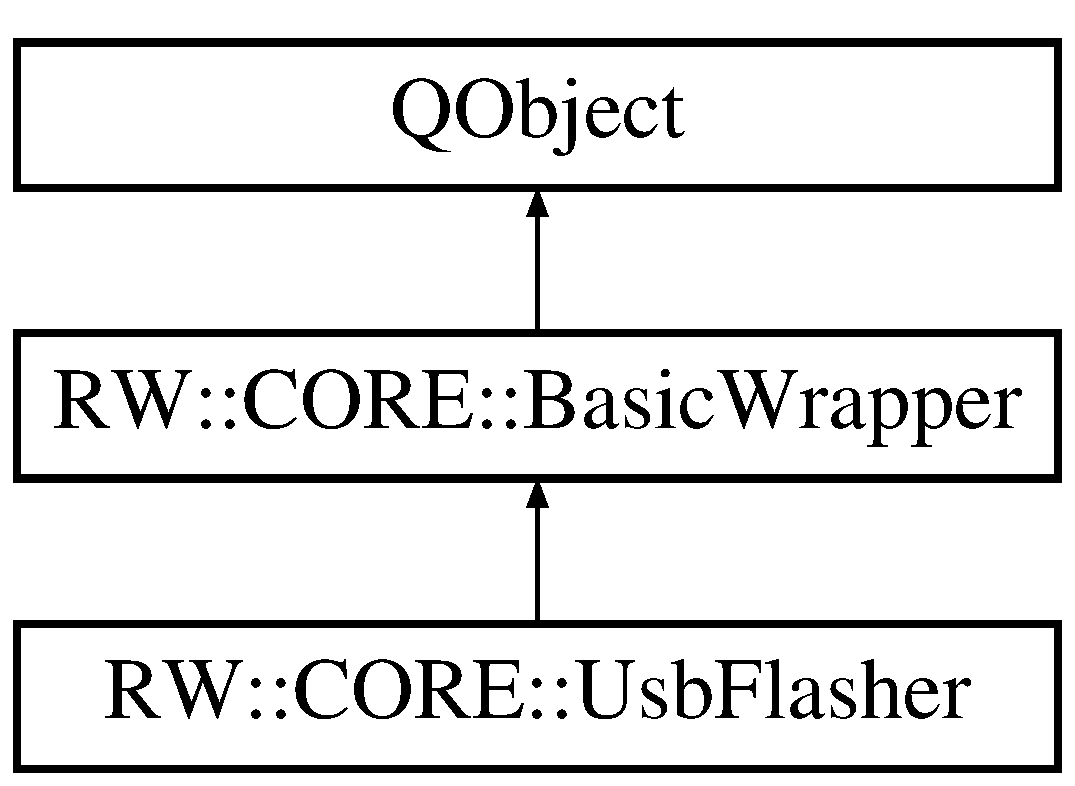
\includegraphics[height=3.000000cm]{class_r_w_1_1_c_o_r_e_1_1_usb_flasher}
\end{center}
\end{figure}
\subsection*{Public Member Functions}
\begin{DoxyCompactItemize}
\item 
\hyperlink{class_r_w_1_1_c_o_r_e_1_1_usb_flasher_a5c10a755b00ae95db557b572445b657c}{Usb\+Flasher} ()
\item 
\hyperlink{class_r_w_1_1_c_o_r_e_1_1_usb_flasher_a8ee30958b7e2fb03a7887f945cfd9698}{$\sim$\+Usb\+Flasher} ()
\end{DoxyCompactItemize}
\subsection*{Additional Inherited Members}


\subsection{Detailed Description}


Definition at line 7 of file Usb\+Flasher.\+h.



\subsection{Constructor \& Destructor Documentation}
\hypertarget{class_r_w_1_1_c_o_r_e_1_1_usb_flasher_a5c10a755b00ae95db557b572445b657c}{}\label{class_r_w_1_1_c_o_r_e_1_1_usb_flasher_a5c10a755b00ae95db557b572445b657c} 
\index{R\+W\+::\+C\+O\+R\+E\+::\+Usb\+Flasher@{R\+W\+::\+C\+O\+R\+E\+::\+Usb\+Flasher}!Usb\+Flasher@{Usb\+Flasher}}
\index{Usb\+Flasher@{Usb\+Flasher}!R\+W\+::\+C\+O\+R\+E\+::\+Usb\+Flasher@{R\+W\+::\+C\+O\+R\+E\+::\+Usb\+Flasher}}
\subsubsection{\texorpdfstring{Usb\+Flasher()}{UsbFlasher()}}
{\footnotesize\ttfamily R\+W\+::\+C\+O\+R\+E\+::\+Usb\+Flasher\+::\+Usb\+Flasher (\begin{DoxyParamCaption}{ }\end{DoxyParamCaption})}



Definition at line 6 of file Usb\+Flasher.\+cpp.

\hypertarget{class_r_w_1_1_c_o_r_e_1_1_usb_flasher_a8ee30958b7e2fb03a7887f945cfd9698}{}\label{class_r_w_1_1_c_o_r_e_1_1_usb_flasher_a8ee30958b7e2fb03a7887f945cfd9698} 
\index{R\+W\+::\+C\+O\+R\+E\+::\+Usb\+Flasher@{R\+W\+::\+C\+O\+R\+E\+::\+Usb\+Flasher}!````~Usb\+Flasher@{$\sim$\+Usb\+Flasher}}
\index{````~Usb\+Flasher@{$\sim$\+Usb\+Flasher}!R\+W\+::\+C\+O\+R\+E\+::\+Usb\+Flasher@{R\+W\+::\+C\+O\+R\+E\+::\+Usb\+Flasher}}
\subsubsection{\texorpdfstring{$\sim$\+Usb\+Flasher()}{~UsbFlasher()}}
{\footnotesize\ttfamily R\+W\+::\+C\+O\+R\+E\+::\+Usb\+Flasher\+::$\sim$\+Usb\+Flasher (\begin{DoxyParamCaption}{ }\end{DoxyParamCaption})}



Definition at line 11 of file Usb\+Flasher.\+cpp.



The documentation for this class was generated from the following files\+:\begin{DoxyCompactItemize}
\item 
C\+:/\+Projekte/\+Remote\+Repros/\+Remote\+Hidden\+Helper/\+Remote\+Hidden\+Helper/\hyperlink{_usb_flasher_8h}{Usb\+Flasher.\+h}\item 
C\+:/\+Projekte/\+Remote\+Repros/\+Remote\+Hidden\+Helper/\+Remote\+Hidden\+Helper/\hyperlink{_usb_flasher_8cpp}{Usb\+Flasher.\+cpp}\end{DoxyCompactItemize}

\chapter{File Documentation}
\hypertarget{_basic_wrapper_8h}{}\section{C\+:/\+Projekte/\+Remote\+Repros/\+Remote\+Hidden\+Helper/\+Remote\+Hidden\+Helper/\+Basic\+Wrapper.h File Reference}
\label{_basic_wrapper_8h}\index{C\+:/\+Projekte/\+Remote\+Repros/\+Remote\+Hidden\+Helper/\+Remote\+Hidden\+Helper/\+Basic\+Wrapper.\+h@{C\+:/\+Projekte/\+Remote\+Repros/\+Remote\+Hidden\+Helper/\+Remote\+Hidden\+Helper/\+Basic\+Wrapper.\+h}}
{\ttfamily \#include \char`\"{}qobject.\+h\char`\"{}}\newline
{\ttfamily \#include \char`\"{}Constants.\+h\char`\"{}}\newline
\subsection*{Classes}
\begin{DoxyCompactItemize}
\item 
class \hyperlink{class_r_w_1_1_c_o_r_e_1_1_basic_wrapper}{R\+W\+::\+C\+O\+R\+E\+::\+Basic\+Wrapper}
\end{DoxyCompactItemize}
\subsection*{Namespaces}
\begin{DoxyCompactItemize}
\item 
 \hyperlink{namespace_r_w}{RW}
\item 
 \hyperlink{namespace_r_w_1_1_c_o_r_e}{R\+W\+::\+C\+O\+RE}
\end{DoxyCompactItemize}

\hypertarget{_can_easy_wrapper_8cpp}{}\section{C\+:/\+Projekte/\+Remote\+Repros/\+Remote\+Hidden\+Helper/\+Remote\+Hidden\+Helper/\+Can\+Easy\+Wrapper.cpp File Reference}
\label{_can_easy_wrapper_8cpp}\index{C\+:/\+Projekte/\+Remote\+Repros/\+Remote\+Hidden\+Helper/\+Remote\+Hidden\+Helper/\+Can\+Easy\+Wrapper.\+cpp@{C\+:/\+Projekte/\+Remote\+Repros/\+Remote\+Hidden\+Helper/\+Remote\+Hidden\+Helper/\+Can\+Easy\+Wrapper.\+cpp}}
{\ttfamily \#include \char`\"{}Can\+Easy\+Wrapper.\+h\char`\"{}}\newline
{\ttfamily \#include $<$qfile.\+h$>$}\newline
{\ttfamily \#include $<$qfileinfo.\+h$>$}\newline
\subsection*{Namespaces}
\begin{DoxyCompactItemize}
\item 
 \hyperlink{namespace_r_w}{RW}
\item 
 \hyperlink{namespace_r_w_1_1_c_o_r_e}{R\+W\+::\+C\+O\+RE}
\end{DoxyCompactItemize}

\hypertarget{_can_easy_wrapper_8h}{}\section{C\+:/\+Projekte/\+Remote\+Repros/\+Remote\+Hidden\+Helper/\+Remote\+Hidden\+Helper/\+Can\+Easy\+Wrapper.h File Reference}
\label{_can_easy_wrapper_8h}\index{C\+:/\+Projekte/\+Remote\+Repros/\+Remote\+Hidden\+Helper/\+Remote\+Hidden\+Helper/\+Can\+Easy\+Wrapper.\+h@{C\+:/\+Projekte/\+Remote\+Repros/\+Remote\+Hidden\+Helper/\+Remote\+Hidden\+Helper/\+Can\+Easy\+Wrapper.\+h}}
{\ttfamily \#include \char`\"{}Basic\+Wrapper.\+h\char`\"{}}\newline
{\ttfamily \#include \char`\"{}atlbase.\+h\char`\"{}}\newline
\subsection*{Classes}
\begin{DoxyCompactItemize}
\item 
class \hyperlink{class_r_w_1_1_c_o_r_e_1_1_can_easy_wrapper}{R\+W\+::\+C\+O\+R\+E\+::\+Can\+Easy\+Wrapper}
\end{DoxyCompactItemize}
\subsection*{Namespaces}
\begin{DoxyCompactItemize}
\item 
 \hyperlink{namespace_r_w}{RW}
\item 
 \hyperlink{namespace_r_w_1_1_c_o_r_e}{R\+W\+::\+C\+O\+RE}
\end{DoxyCompactItemize}

\hypertarget{_communication_manager_8cpp}{}\section{C\+:/\+Projekte/\+Remote\+Repros/\+Remote\+Hidden\+Helper/\+Remote\+Hidden\+Helper/\+Communication\+Manager.cpp File Reference}
\label{_communication_manager_8cpp}\index{C\+:/\+Projekte/\+Remote\+Repros/\+Remote\+Hidden\+Helper/\+Remote\+Hidden\+Helper/\+Communication\+Manager.\+cpp@{C\+:/\+Projekte/\+Remote\+Repros/\+Remote\+Hidden\+Helper/\+Remote\+Hidden\+Helper/\+Communication\+Manager.\+cpp}}
{\ttfamily \#include \char`\"{}Communication\+Manager.\+h\char`\"{}}\newline
{\ttfamily \#include \char`\"{}Communication\+Server.\+h\char`\"{}}\newline
{\ttfamily \#include \char`\"{}Error\+Handler.\+h\char`\"{}}\newline
{\ttfamily \#include \char`\"{}Util.\+h\char`\"{}}\newline
\subsection*{Namespaces}
\begin{DoxyCompactItemize}
\item 
 \hyperlink{namespace_r_w}{RW}
\item 
 \hyperlink{namespace_r_w_1_1_c_o_r_e}{R\+W\+::\+C\+O\+RE}
\end{DoxyCompactItemize}

\hypertarget{_communication_manager_8h}{}\section{C\+:/\+Projekte/\+Remote\+Repros/\+Remote\+Hidden\+Helper/\+Remote\+Hidden\+Helper/\+Communication\+Manager.h File Reference}
\label{_communication_manager_8h}\index{C\+:/\+Projekte/\+Remote\+Repros/\+Remote\+Hidden\+Helper/\+Remote\+Hidden\+Helper/\+Communication\+Manager.\+h@{C\+:/\+Projekte/\+Remote\+Repros/\+Remote\+Hidden\+Helper/\+Remote\+Hidden\+Helper/\+Communication\+Manager.\+h}}
{\ttfamily \#include $<$Qt\+Core$>$}\newline
{\ttfamily \#include \char`\"{}Constants.\+h\char`\"{}}\newline
\subsection*{Classes}
\begin{DoxyCompactItemize}
\item 
class \hyperlink{class_r_w_1_1_c_o_r_e_1_1_communication_manager}{R\+W\+::\+C\+O\+R\+E\+::\+Communication\+Manager}
\end{DoxyCompactItemize}
\subsection*{Namespaces}
\begin{DoxyCompactItemize}
\item 
 \hyperlink{namespace_r_w}{RW}
\item 
 \hyperlink{namespace_r_w_1_1_c_o_r_e}{R\+W\+::\+C\+O\+RE}
\end{DoxyCompactItemize}

\hypertarget{_communication_server_8cpp}{}\section{C\+:/\+Projekte/\+Remote\+Repros/\+Remote\+Hidden\+Helper/\+Remote\+Hidden\+Helper/\+Communication\+Server.cpp File Reference}
\label{_communication_server_8cpp}\index{C\+:/\+Projekte/\+Remote\+Repros/\+Remote\+Hidden\+Helper/\+Remote\+Hidden\+Helper/\+Communication\+Server.\+cpp@{C\+:/\+Projekte/\+Remote\+Repros/\+Remote\+Hidden\+Helper/\+Remote\+Hidden\+Helper/\+Communication\+Server.\+cpp}}
{\ttfamily \#include \char`\"{}Communication\+Server.\+h\char`\"{}}\newline
{\ttfamily \#include \char`\"{}Util.\+h\char`\"{}}\newline
\subsection*{Namespaces}
\begin{DoxyCompactItemize}
\item 
 \hyperlink{namespace_r_w}{RW}
\item 
 \hyperlink{namespace_r_w_1_1_c_o_r_e}{R\+W\+::\+C\+O\+RE}
\end{DoxyCompactItemize}

\hypertarget{_communication_server_8h}{}\section{C\+:/\+Projekte/\+Remote\+Repros/\+Remote\+Hidden\+Helper/\+Remote\+Hidden\+Helper/\+Communication\+Server.h File Reference}
\label{_communication_server_8h}\index{C\+:/\+Projekte/\+Remote\+Repros/\+Remote\+Hidden\+Helper/\+Remote\+Hidden\+Helper/\+Communication\+Server.\+h@{C\+:/\+Projekte/\+Remote\+Repros/\+Remote\+Hidden\+Helper/\+Remote\+Hidden\+Helper/\+Communication\+Server.\+h}}
{\ttfamily \#include $<$Q\+Local\+Server$>$}\newline
{\ttfamily \#include $<$Q\+Local\+Socket$>$}\newline
{\ttfamily \#include $<$qdatastream.\+h$>$}\newline
{\ttfamily \#include \char`\"{}Constants.\+h\char`\"{}}\newline
\subsection*{Classes}
\begin{DoxyCompactItemize}
\item 
class \hyperlink{class_r_w_1_1_c_o_r_e_1_1_communication_server}{R\+W\+::\+C\+O\+R\+E\+::\+Communication\+Server}
\end{DoxyCompactItemize}
\subsection*{Namespaces}
\begin{DoxyCompactItemize}
\item 
 \hyperlink{namespace_r_w}{RW}
\item 
 \hyperlink{namespace_r_w_1_1_c_o_r_e}{R\+W\+::\+C\+O\+RE}
\end{DoxyCompactItemize}
\subsection*{Variables}
\begin{DoxyCompactItemize}
\item 
const Q\+String \hyperlink{namespace_r_w_1_1_c_o_r_e_adaaf185681c4c91a7d72836e233b6088}{R\+W\+::\+C\+O\+R\+E\+::\+Socket\+Name} = \char`\"{}remotehiddenhelper\char`\"{}
\end{DoxyCompactItemize}

\hypertarget{_constant_8h}{}\section{C\+:/\+Projekte/\+Remote\+Repros/\+Remote\+Hidden\+Helper/\+Remote\+Hidden\+Helper/\+Constant.h File Reference}
\label{_constant_8h}\index{C\+:/\+Projekte/\+Remote\+Repros/\+Remote\+Hidden\+Helper/\+Remote\+Hidden\+Helper/\+Constant.\+h@{C\+:/\+Projekte/\+Remote\+Repros/\+Remote\+Hidden\+Helper/\+Remote\+Hidden\+Helper/\+Constant.\+h}}
\subsection*{Namespaces}
\begin{DoxyCompactItemize}
\item 
 \hyperlink{namespace_r_w}{RW}
\item 
 \hyperlink{namespace_r_w_1_1_c_o_r_e}{R\+W\+::\+C\+O\+RE}
\end{DoxyCompactItemize}

\hypertarget{_constants_8h}{}\section{C\+:/\+Projekte/\+Remote\+Repros/\+Remote\+Hidden\+Helper/\+Remote\+Hidden\+Helper/\+Constants.h File Reference}
\label{_constants_8h}\index{C\+:/\+Projekte/\+Remote\+Repros/\+Remote\+Hidden\+Helper/\+Remote\+Hidden\+Helper/\+Constants.\+h@{C\+:/\+Projekte/\+Remote\+Repros/\+Remote\+Hidden\+Helper/\+Remote\+Hidden\+Helper/\+Constants.\+h}}
{\ttfamily \#include $<$qobject.\+h$>$}\newline
\subsection*{Classes}
\begin{DoxyCompactItemize}
\item 
struct \hyperlink{struct_r_w_1_1_c_o_r_e_1_1___message}{R\+W\+::\+C\+O\+R\+E\+::\+\_\+\+Message}
\end{DoxyCompactItemize}
\subsection*{Namespaces}
\begin{DoxyCompactItemize}
\item 
 \hyperlink{namespace_r_w}{RW}
\item 
 \hyperlink{namespace_r_w_1_1_c_o_r_e}{R\+W\+::\+C\+O\+RE}
\end{DoxyCompactItemize}
\subsection*{Typedefs}
\begin{DoxyCompactItemize}
\item 
typedef struct \hyperlink{struct_r_w_1_1_c_o_r_e_1_1___message}{R\+W\+::\+C\+O\+R\+E\+::\+\_\+\+Message} \hyperlink{namespace_r_w_1_1_c_o_r_e_a571834b44d0e3fab58aa6abfe5a02988}{R\+W\+::\+C\+O\+R\+E\+::\+Message}
\end{DoxyCompactItemize}
\subsection*{Enumerations}
\begin{DoxyCompactItemize}
\item 
enum \hyperlink{namespace_r_w_1_1_c_o_r_e_a46e6ab0e8b9b71a2b5c8dc4a84e3f81c}{R\+W\+::\+C\+O\+R\+E\+::\+Message\+Receiver} \{ \newline
\hyperlink{namespace_r_w_1_1_c_o_r_e_a46e6ab0e8b9b71a2b5c8dc4a84e3f81caa45b74cb40c140aa525c7cec9cebe852}{R\+W\+::\+C\+O\+R\+E\+::\+Message\+Receiver\+::\+Communication\+Server}, 
\hyperlink{namespace_r_w_1_1_c_o_r_e_a46e6ab0e8b9b71a2b5c8dc4a84e3f81ca555daea5d6d0abdadcdafef77d26b117}{R\+W\+::\+C\+O\+R\+E\+::\+Message\+Receiver\+::\+Process\+Manager}, 
\hyperlink{namespace_r_w_1_1_c_o_r_e_a46e6ab0e8b9b71a2b5c8dc4a84e3f81ca36dfa730942a10c1ce7c46cc009c767a}{R\+W\+::\+C\+O\+R\+E\+::\+Message\+Receiver\+::\+Can\+Easy\+Wrapper}, 
\hyperlink{namespace_r_w_1_1_c_o_r_e_a46e6ab0e8b9b71a2b5c8dc4a84e3f81cab92348e2791b0ba8e28b0827deb085f0}{R\+W\+::\+C\+O\+R\+E\+::\+Message\+Receiver\+::\+Basic\+Wrapper}, 
\newline
\hyperlink{namespace_r_w_1_1_c_o_r_e_a46e6ab0e8b9b71a2b5c8dc4a84e3f81ca2acab22f8d8fee7dd115aa43789c298b}{R\+W\+::\+C\+O\+R\+E\+::\+Message\+Receiver\+::\+Portal\+Info}, 
\hyperlink{namespace_r_w_1_1_c_o_r_e_a46e6ab0e8b9b71a2b5c8dc4a84e3f81ca5a057456c3c7f0a5c154d9a9604d5961}{R\+W\+::\+C\+O\+R\+E\+::\+Message\+Receiver\+::\+F\+Host\+S\+P\+Wrapper}, 
\hyperlink{namespace_r_w_1_1_c_o_r_e_a46e6ab0e8b9b71a2b5c8dc4a84e3f81cadf6f388021247e2e23a0655101c62eaa}{R\+W\+::\+C\+O\+R\+E\+::\+Message\+Receiver\+::\+M\+K\+S\+Wrapper}, 
\hyperlink{namespace_r_w_1_1_c_o_r_e_a46e6ab0e8b9b71a2b5c8dc4a84e3f81caa45b74cb40c140aa525c7cec9cebe852}{R\+W\+::\+C\+O\+R\+E\+::\+Message\+Receiver\+::\+Communication\+Server}, 
\newline
\hyperlink{namespace_r_w_1_1_c_o_r_e_a46e6ab0e8b9b71a2b5c8dc4a84e3f81ca555daea5d6d0abdadcdafef77d26b117}{R\+W\+::\+C\+O\+R\+E\+::\+Message\+Receiver\+::\+Process\+Manager}, 
\hyperlink{namespace_r_w_1_1_c_o_r_e_a46e6ab0e8b9b71a2b5c8dc4a84e3f81ca36dfa730942a10c1ce7c46cc009c767a}{R\+W\+::\+C\+O\+R\+E\+::\+Message\+Receiver\+::\+Can\+Easy\+Wrapper}, 
\hyperlink{namespace_r_w_1_1_c_o_r_e_a46e6ab0e8b9b71a2b5c8dc4a84e3f81cab92348e2791b0ba8e28b0827deb085f0}{R\+W\+::\+C\+O\+R\+E\+::\+Message\+Receiver\+::\+Basic\+Wrapper}, 
\hyperlink{namespace_r_w_1_1_c_o_r_e_a46e6ab0e8b9b71a2b5c8dc4a84e3f81ca2acab22f8d8fee7dd115aa43789c298b}{R\+W\+::\+C\+O\+R\+E\+::\+Message\+Receiver\+::\+Portal\+Info}, 
\newline
\hyperlink{namespace_r_w_1_1_c_o_r_e_a46e6ab0e8b9b71a2b5c8dc4a84e3f81ca5a057456c3c7f0a5c154d9a9604d5961}{R\+W\+::\+C\+O\+R\+E\+::\+Message\+Receiver\+::\+F\+Host\+S\+P\+Wrapper}, 
\hyperlink{namespace_r_w_1_1_c_o_r_e_a46e6ab0e8b9b71a2b5c8dc4a84e3f81cadf6f388021247e2e23a0655101c62eaa}{R\+W\+::\+C\+O\+R\+E\+::\+Message\+Receiver\+::\+M\+K\+S\+Wrapper}
 \}
\item 
enum \hyperlink{namespace_r_w_1_1_c_o_r_e_ac0e275b436280ccfd1c33476ca8ff9c6}{R\+W\+::\+C\+O\+R\+E\+::\+Functions} \{ \newline
\hyperlink{namespace_r_w_1_1_c_o_r_e_ac0e275b436280ccfd1c33476ca8ff9c6a68ea1e2ad2d63d222a1add53cbf70a55}{R\+W\+::\+C\+O\+R\+E\+::\+Functions\+::\+Can\+Easy\+Start\+Application}, 
\hyperlink{namespace_r_w_1_1_c_o_r_e_ac0e275b436280ccfd1c33476ca8ff9c6a29e4b3929d9d327ea6a1dd5c56a6681e}{R\+W\+::\+C\+O\+R\+E\+::\+Functions\+::\+Can\+Easy\+Load\+Workspace}, 
\hyperlink{namespace_r_w_1_1_c_o_r_e_ac0e275b436280ccfd1c33476ca8ff9c6aa8a2e5b03905a3b9cc5efa079095665b}{R\+W\+::\+C\+O\+R\+E\+::\+Functions\+::\+Can\+Easy\+Close\+Application}, 
\hyperlink{namespace_r_w_1_1_c_o_r_e_ac0e275b436280ccfd1c33476ca8ff9c6a6d6d9768e6b5ce9d737e19532967ea0e}{R\+W\+::\+C\+O\+R\+E\+::\+Functions\+::\+Can\+Easy\+Start\+Simulation}, 
\newline
\hyperlink{namespace_r_w_1_1_c_o_r_e_ac0e275b436280ccfd1c33476ca8ff9c6a494f84cef80750fba24fbbba6198c3a1}{R\+W\+::\+C\+O\+R\+E\+::\+Functions\+::\+Can\+Easy\+Stop\+Simulation}, 
\hyperlink{namespace_r_w_1_1_c_o_r_e_ac0e275b436280ccfd1c33476ca8ff9c6a416cee9214b8ccb2871ffdd16caf979e}{R\+W\+::\+C\+O\+R\+E\+::\+Functions\+::\+M\+K\+S\+Login}, 
\hyperlink{namespace_r_w_1_1_c_o_r_e_ac0e275b436280ccfd1c33476ca8ff9c6a962a894f82d4083c9ed0c86ba83579f1}{R\+W\+::\+C\+O\+R\+E\+::\+Functions\+::\+M\+K\+S\+Start\+Download}, 
\hyperlink{namespace_r_w_1_1_c_o_r_e_ac0e275b436280ccfd1c33476ca8ff9c6acb8ca8a616069c87e37bb8d729cb02d0}{R\+W\+::\+C\+O\+R\+E\+::\+Functions\+::\+M\+K\+S\+Create\+Sand\+Box}, 
\newline
\hyperlink{namespace_r_w_1_1_c_o_r_e_ac0e275b436280ccfd1c33476ca8ff9c6a595d390c905a10fe130b1e65ee60d409}{R\+W\+::\+C\+O\+R\+E\+::\+Functions\+::\+M\+K\+S\+Drop\+Sandbox}, 
\hyperlink{namespace_r_w_1_1_c_o_r_e_ac0e275b436280ccfd1c33476ca8ff9c6a53b95d5a629256700ee4800668b3f279}{R\+W\+::\+C\+O\+R\+E\+::\+Functions\+::\+F\+Host\+S\+P\+Start\+F\+Host}, 
\hyperlink{namespace_r_w_1_1_c_o_r_e_ac0e275b436280ccfd1c33476ca8ff9c6a489b7daa856bd0c04cba47b80d8b129e}{R\+W\+::\+C\+O\+R\+E\+::\+Functions\+::\+F\+Host\+S\+P\+Load\+Flash\+File}, 
\hyperlink{namespace_r_w_1_1_c_o_r_e_ac0e275b436280ccfd1c33476ca8ff9c6af394b756e27e873e06babc42f5ce16ad}{R\+W\+::\+C\+O\+R\+E\+::\+Functions\+::\+F\+Host\+S\+P\+Close\+F\+Host}, 
\newline
\hyperlink{namespace_r_w_1_1_c_o_r_e_ac0e275b436280ccfd1c33476ca8ff9c6af3191856437334bd4d909109b6308803}{R\+W\+::\+C\+O\+R\+E\+::\+Functions\+::\+F\+Host\+S\+P\+Get\+State}, 
\hyperlink{namespace_r_w_1_1_c_o_r_e_ac0e275b436280ccfd1c33476ca8ff9c6a07b25718c7dcc2e93cfd6f0688443856}{R\+W\+::\+C\+O\+R\+E\+::\+Functions\+::\+F\+Host\+S\+P\+Abort\+Sequence}, 
\hyperlink{namespace_r_w_1_1_c_o_r_e_ac0e275b436280ccfd1c33476ca8ff9c6afdbe3c72b88662d5273abce87674bf60}{R\+W\+::\+C\+O\+R\+E\+::\+Functions\+::\+F\+Host\+S\+P\+Close\+Sequence}, 
\hyperlink{namespace_r_w_1_1_c_o_r_e_ac0e275b436280ccfd1c33476ca8ff9c6a75492f3471b2e122c0aa20fcb7c630de}{R\+W\+::\+C\+O\+R\+E\+::\+Functions\+::\+F\+Host\+S\+P\+Start\+Flash}, 
\newline
\hyperlink{namespace_r_w_1_1_c_o_r_e_ac0e275b436280ccfd1c33476ca8ff9c6afb4b8ca4a5eb814655e4cfc298c9196a}{R\+W\+::\+C\+O\+R\+E\+::\+Functions\+::\+F\+Host\+S\+P\+Get\+Progress}, 
\hyperlink{namespace_r_w_1_1_c_o_r_e_ac0e275b436280ccfd1c33476ca8ff9c6ac5de6f51437461690c316959c19e735f}{R\+W\+::\+C\+O\+R\+E\+::\+Functions\+::\+Portal\+Info\+Fitting\+AC}, 
\hyperlink{namespace_r_w_1_1_c_o_r_e_ac0e275b436280ccfd1c33476ca8ff9c6adbcc70a6cd5b5fae96445878563ce253}{R\+W\+::\+C\+O\+R\+E\+::\+Functions\+::\+Portal\+Info\+Ac\+By\+Icom}, 
\hyperlink{namespace_r_w_1_1_c_o_r_e_ac0e275b436280ccfd1c33476ca8ff9c6ab8dba7b66a9709df87e9e1a7e47f270d}{R\+W\+::\+C\+O\+R\+E\+::\+Functions\+::\+Portal\+Info\+Releases}, 
\newline
\hyperlink{namespace_r_w_1_1_c_o_r_e_ac0e275b436280ccfd1c33476ca8ff9c6a26255bc19d2110541c084e79e9e0ebf6}{R\+W\+::\+C\+O\+R\+E\+::\+Functions\+::\+Portal\+Info\+Software\+By\+Id}, 
\hyperlink{namespace_r_w_1_1_c_o_r_e_ac0e275b436280ccfd1c33476ca8ff9c6a540bf47a5430268dddefa13988d5c188}{R\+W\+::\+C\+O\+R\+E\+::\+Functions\+::\+Portal\+Info\+Show\+Dialog}, 
\hyperlink{namespace_r_w_1_1_c_o_r_e_ac0e275b436280ccfd1c33476ca8ff9c6ad58d7de7a3f9e64ea339c50d31238cf7}{R\+W\+::\+C\+O\+R\+E\+::\+Functions\+::\+Portal\+Info\+Close\+Dialog}, 
\hyperlink{namespace_r_w_1_1_c_o_r_e_ac0e275b436280ccfd1c33476ca8ff9c6ab2f40690858b404ed10e62bdf422c704}{R\+W\+::\+C\+O\+R\+E\+::\+Functions\+::\+Amount}, 
\newline
\hyperlink{namespace_r_w_1_1_c_o_r_e_ac0e275b436280ccfd1c33476ca8ff9c6a68ea1e2ad2d63d222a1add53cbf70a55}{R\+W\+::\+C\+O\+R\+E\+::\+Functions\+::\+Can\+Easy\+Start\+Application}, 
\hyperlink{namespace_r_w_1_1_c_o_r_e_ac0e275b436280ccfd1c33476ca8ff9c6a29e4b3929d9d327ea6a1dd5c56a6681e}{R\+W\+::\+C\+O\+R\+E\+::\+Functions\+::\+Can\+Easy\+Load\+Workspace}, 
\hyperlink{namespace_r_w_1_1_c_o_r_e_ac0e275b436280ccfd1c33476ca8ff9c6aa8a2e5b03905a3b9cc5efa079095665b}{R\+W\+::\+C\+O\+R\+E\+::\+Functions\+::\+Can\+Easy\+Close\+Application}, 
\hyperlink{namespace_r_w_1_1_c_o_r_e_ac0e275b436280ccfd1c33476ca8ff9c6a6d6d9768e6b5ce9d737e19532967ea0e}{R\+W\+::\+C\+O\+R\+E\+::\+Functions\+::\+Can\+Easy\+Start\+Simulation}, 
\newline
\hyperlink{namespace_r_w_1_1_c_o_r_e_ac0e275b436280ccfd1c33476ca8ff9c6a494f84cef80750fba24fbbba6198c3a1}{R\+W\+::\+C\+O\+R\+E\+::\+Functions\+::\+Can\+Easy\+Stop\+Simulation}, 
\hyperlink{namespace_r_w_1_1_c_o_r_e_ac0e275b436280ccfd1c33476ca8ff9c6a416cee9214b8ccb2871ffdd16caf979e}{R\+W\+::\+C\+O\+R\+E\+::\+Functions\+::\+M\+K\+S\+Login}, 
\hyperlink{namespace_r_w_1_1_c_o_r_e_ac0e275b436280ccfd1c33476ca8ff9c6a962a894f82d4083c9ed0c86ba83579f1}{R\+W\+::\+C\+O\+R\+E\+::\+Functions\+::\+M\+K\+S\+Start\+Download}, 
\hyperlink{namespace_r_w_1_1_c_o_r_e_ac0e275b436280ccfd1c33476ca8ff9c6acb8ca8a616069c87e37bb8d729cb02d0}{R\+W\+::\+C\+O\+R\+E\+::\+Functions\+::\+M\+K\+S\+Create\+Sand\+Box}, 
\newline
\hyperlink{namespace_r_w_1_1_c_o_r_e_ac0e275b436280ccfd1c33476ca8ff9c6a595d390c905a10fe130b1e65ee60d409}{R\+W\+::\+C\+O\+R\+E\+::\+Functions\+::\+M\+K\+S\+Drop\+Sandbox}, 
\hyperlink{namespace_r_w_1_1_c_o_r_e_ac0e275b436280ccfd1c33476ca8ff9c6a53b95d5a629256700ee4800668b3f279}{R\+W\+::\+C\+O\+R\+E\+::\+Functions\+::\+F\+Host\+S\+P\+Start\+F\+Host}, 
\hyperlink{namespace_r_w_1_1_c_o_r_e_ac0e275b436280ccfd1c33476ca8ff9c6a489b7daa856bd0c04cba47b80d8b129e}{R\+W\+::\+C\+O\+R\+E\+::\+Functions\+::\+F\+Host\+S\+P\+Load\+Flash\+File}, 
\hyperlink{namespace_r_w_1_1_c_o_r_e_ac0e275b436280ccfd1c33476ca8ff9c6af394b756e27e873e06babc42f5ce16ad}{R\+W\+::\+C\+O\+R\+E\+::\+Functions\+::\+F\+Host\+S\+P\+Close\+F\+Host}, 
\newline
\hyperlink{namespace_r_w_1_1_c_o_r_e_ac0e275b436280ccfd1c33476ca8ff9c6af3191856437334bd4d909109b6308803}{R\+W\+::\+C\+O\+R\+E\+::\+Functions\+::\+F\+Host\+S\+P\+Get\+State}, 
\hyperlink{namespace_r_w_1_1_c_o_r_e_ac0e275b436280ccfd1c33476ca8ff9c6a07b25718c7dcc2e93cfd6f0688443856}{R\+W\+::\+C\+O\+R\+E\+::\+Functions\+::\+F\+Host\+S\+P\+Abort\+Sequence}, 
\hyperlink{namespace_r_w_1_1_c_o_r_e_ac0e275b436280ccfd1c33476ca8ff9c6afdbe3c72b88662d5273abce87674bf60}{R\+W\+::\+C\+O\+R\+E\+::\+Functions\+::\+F\+Host\+S\+P\+Close\+Sequence}, 
\hyperlink{namespace_r_w_1_1_c_o_r_e_ac0e275b436280ccfd1c33476ca8ff9c6a75492f3471b2e122c0aa20fcb7c630de}{R\+W\+::\+C\+O\+R\+E\+::\+Functions\+::\+F\+Host\+S\+P\+Start\+Flash}, 
\newline
\hyperlink{namespace_r_w_1_1_c_o_r_e_ac0e275b436280ccfd1c33476ca8ff9c6afb4b8ca4a5eb814655e4cfc298c9196a}{R\+W\+::\+C\+O\+R\+E\+::\+Functions\+::\+F\+Host\+S\+P\+Get\+Progress}, 
\hyperlink{namespace_r_w_1_1_c_o_r_e_ac0e275b436280ccfd1c33476ca8ff9c6ac5de6f51437461690c316959c19e735f}{R\+W\+::\+C\+O\+R\+E\+::\+Functions\+::\+Portal\+Info\+Fitting\+AC}, 
\hyperlink{namespace_r_w_1_1_c_o_r_e_ac0e275b436280ccfd1c33476ca8ff9c6adbcc70a6cd5b5fae96445878563ce253}{R\+W\+::\+C\+O\+R\+E\+::\+Functions\+::\+Portal\+Info\+Ac\+By\+Icom}, 
\hyperlink{namespace_r_w_1_1_c_o_r_e_ac0e275b436280ccfd1c33476ca8ff9c6ab8dba7b66a9709df87e9e1a7e47f270d}{R\+W\+::\+C\+O\+R\+E\+::\+Functions\+::\+Portal\+Info\+Releases}, 
\newline
\hyperlink{namespace_r_w_1_1_c_o_r_e_ac0e275b436280ccfd1c33476ca8ff9c6a26255bc19d2110541c084e79e9e0ebf6}{R\+W\+::\+C\+O\+R\+E\+::\+Functions\+::\+Portal\+Info\+Software\+By\+Id}, 
\hyperlink{namespace_r_w_1_1_c_o_r_e_ac0e275b436280ccfd1c33476ca8ff9c6a540bf47a5430268dddefa13988d5c188}{R\+W\+::\+C\+O\+R\+E\+::\+Functions\+::\+Portal\+Info\+Show\+Dialog}, 
\hyperlink{namespace_r_w_1_1_c_o_r_e_ac0e275b436280ccfd1c33476ca8ff9c6ad58d7de7a3f9e64ea339c50d31238cf7}{R\+W\+::\+C\+O\+R\+E\+::\+Functions\+::\+Portal\+Info\+Close\+Dialog}, 
\hyperlink{namespace_r_w_1_1_c_o_r_e_ac0e275b436280ccfd1c33476ca8ff9c6ab2f40690858b404ed10e62bdf422c704}{R\+W\+::\+C\+O\+R\+E\+::\+Functions\+::\+Amount}
 \}
\item 
enum \hyperlink{namespace_r_w_1_1_c_o_r_e_adc31704b5171629bde8ad1b0badc49d4}{R\+W\+::\+C\+O\+R\+E\+::\+Error\+ID} \{ \newline
\hyperlink{namespace_r_w_1_1_c_o_r_e_adc31704b5171629bde8ad1b0badc49d4a505a83f220c02df2f85c3810cd9ceb38}{R\+W\+::\+C\+O\+R\+E\+::\+Error\+I\+D\+::\+Success}, 
\hyperlink{namespace_r_w_1_1_c_o_r_e_adc31704b5171629bde8ad1b0badc49d4a902b0d55fddef6f8d651fe1035b7d4bd}{R\+W\+::\+C\+O\+R\+E\+::\+Error\+I\+D\+::\+Error}, 
\hyperlink{namespace_r_w_1_1_c_o_r_e_adc31704b5171629bde8ad1b0badc49d4ad8a942ef2b04672adfafef0ad817a407}{R\+W\+::\+C\+O\+R\+E\+::\+Error\+I\+D\+::\+Busy}, 
\hyperlink{namespace_r_w_1_1_c_o_r_e_adc31704b5171629bde8ad1b0badc49d4aadcae2e0054a8ba193997e36dabb670c}{R\+W\+::\+C\+O\+R\+E\+::\+Error\+I\+D\+::\+Error\+Can\+Easy\+Com\+Server\+Missing}, 
\newline
\hyperlink{namespace_r_w_1_1_c_o_r_e_adc31704b5171629bde8ad1b0badc49d4a1aad633e213deab4243b2d5999c2360b}{R\+W\+::\+C\+O\+R\+E\+::\+Error\+I\+D\+::\+Error\+Can\+Easy\+Start\+Simulation}, 
\hyperlink{namespace_r_w_1_1_c_o_r_e_adc31704b5171629bde8ad1b0badc49d4a67b965eb5d2714ffad43574db01bbe36}{R\+W\+::\+C\+O\+R\+E\+::\+Error\+I\+D\+::\+Error\+Can\+Easy\+Simulation\+Is\+Running\+Failed}, 
\hyperlink{namespace_r_w_1_1_c_o_r_e_adc31704b5171629bde8ad1b0badc49d4a8de3c8bb0e59da0a13a674f231484209}{R\+W\+::\+C\+O\+R\+E\+::\+Error\+I\+D\+::\+Error\+Can\+Easy\+Stop\+Simulation}, 
\hyperlink{namespace_r_w_1_1_c_o_r_e_adc31704b5171629bde8ad1b0badc49d4a65c84ef98637b7d833ec2e2ee67ea425}{R\+W\+::\+C\+O\+R\+E\+::\+Error\+I\+D\+::\+Error\+Can\+Easy\+Workspace\+Not\+Found}, 
\newline
\hyperlink{namespace_r_w_1_1_c_o_r_e_adc31704b5171629bde8ad1b0badc49d4a17e0d141677302dbedc97f98e5b04c5d}{R\+W\+::\+C\+O\+R\+E\+::\+Error\+I\+D\+::\+Error\+Can\+Easy\+Workspace\+Not\+Loaded}, 
\hyperlink{namespace_r_w_1_1_c_o_r_e_adc31704b5171629bde8ad1b0badc49d4a005b86d6c782938015e999e88dd11cb0}{R\+W\+::\+C\+O\+R\+E\+::\+Error\+I\+D\+::\+Error\+Can\+Easy\+Application\+Error}, 
\hyperlink{namespace_r_w_1_1_c_o_r_e_adc31704b5171629bde8ad1b0badc49d4aebc41f539917e3be033d2ba01e60e5a9}{R\+W\+::\+C\+O\+R\+E\+::\+Error\+I\+D\+::\+Error\+Can\+Easy\+De\+Init\+Error}, 
\hyperlink{namespace_r_w_1_1_c_o_r_e_adc31704b5171629bde8ad1b0badc49d4a8a6a13d1967b6dded3a08bde36a74420}{R\+W\+::\+C\+O\+R\+E\+::\+Error\+I\+D\+::\+Error\+M\+K\+S\+Location\+Missing}, 
\newline
\hyperlink{namespace_r_w_1_1_c_o_r_e_adc31704b5171629bde8ad1b0badc49d4a386333c85d285a2cd50103b4d84a174d}{R\+W\+::\+C\+O\+R\+E\+::\+Error\+I\+D\+::\+Error\+M\+K\+S\+Error}, 
\hyperlink{namespace_r_w_1_1_c_o_r_e_adc31704b5171629bde8ad1b0badc49d4abf1fff945513f28c91a3992f8abe9183}{R\+W\+::\+C\+O\+R\+E\+::\+Error\+I\+D\+::\+Error\+M\+K\+S\+Sand\+Box\+Creation}, 
\hyperlink{namespace_r_w_1_1_c_o_r_e_adc31704b5171629bde8ad1b0badc49d4a00c66c1f833d0c99e277acd53300281f}{R\+W\+::\+C\+O\+R\+E\+::\+Error\+I\+D\+::\+Error\+M\+K\+S\+Sanb\+Box\+Drop}, 
\hyperlink{namespace_r_w_1_1_c_o_r_e_adc31704b5171629bde8ad1b0badc49d4a99318f5ce864699b1063c096d8ee303d}{R\+W\+::\+C\+O\+R\+E\+::\+Error\+I\+D\+::\+Error\+M\+K\+S\+Missing\+Parameter}, 
\newline
\hyperlink{namespace_r_w_1_1_c_o_r_e_adc31704b5171629bde8ad1b0badc49d4ae14b8a20dc980427835211d6857b8824}{R\+W\+::\+C\+O\+R\+E\+::\+Error\+I\+D\+::\+Error\+F\+Host\+S\+P\+Start\+Application}, 
\hyperlink{namespace_r_w_1_1_c_o_r_e_adc31704b5171629bde8ad1b0badc49d4a2bed3be5eff6e78c2f6cd9800c1e8e93}{R\+W\+::\+C\+O\+R\+E\+::\+Error\+I\+D\+::\+Error\+F\+Host\+S\+P\+Sequence\+Stop}, 
\hyperlink{namespace_r_w_1_1_c_o_r_e_adc31704b5171629bde8ad1b0badc49d4a5d1f54c733c971f9652069e6334dc295}{R\+W\+::\+C\+O\+R\+E\+::\+Error\+I\+D\+::\+Error\+F\+Host\+S\+P\+Sequence\+Start}, 
\hyperlink{namespace_r_w_1_1_c_o_r_e_adc31704b5171629bde8ad1b0badc49d4ad4f043489b9b90978e2cab65d0964382}{R\+W\+::\+C\+O\+R\+E\+::\+Error\+I\+D\+::\+Error\+F\+Host\+S\+P\+Load\+Flashfile\+Status\+Failed}, 
\newline
\hyperlink{namespace_r_w_1_1_c_o_r_e_adc31704b5171629bde8ad1b0badc49d4a1da6e55d019a8298dcfdb47e7818689a}{R\+W\+::\+C\+O\+R\+E\+::\+Error\+I\+D\+::\+Error\+F\+Host\+S\+P\+Load\+Flashfile\+Failed}, 
\hyperlink{namespace_r_w_1_1_c_o_r_e_adc31704b5171629bde8ad1b0badc49d4a12ecaf63d3eaea1a1ff04f7bc0c593e2}{R\+W\+::\+C\+O\+R\+E\+::\+Error\+I\+D\+::\+Error\+F\+Host\+S\+P\+Flashfile\+Not\+Exits}, 
\hyperlink{namespace_r_w_1_1_c_o_r_e_adc31704b5171629bde8ad1b0badc49d4a9b494a5bb0810aa0cc1f7100f35b7988}{R\+W\+::\+C\+O\+R\+E\+::\+Error\+I\+D\+::\+Error\+F\+Host\+S\+P\+Get\+Progress}, 
\hyperlink{namespace_r_w_1_1_c_o_r_e_adc31704b5171629bde8ad1b0badc49d4a2f05de453407ec05df087462a416d0c9}{R\+W\+::\+C\+O\+R\+E\+::\+Error\+I\+D\+::\+Error\+F\+Host\+S\+P\+Close\+Application}, 
\newline
\hyperlink{namespace_r_w_1_1_c_o_r_e_adc31704b5171629bde8ad1b0badc49d4af6389f23c6f53163ef63a17a357452f5}{R\+W\+::\+C\+O\+R\+E\+::\+Error\+I\+D\+::\+Error\+F\+Host\+S\+P\+Get\+State\+Failed}, 
\hyperlink{namespace_r_w_1_1_c_o_r_e_adc31704b5171629bde8ad1b0badc49d4a8726d6b328c4beb34762e3f02da1cf72}{R\+W\+::\+C\+O\+R\+E\+::\+Error\+I\+D\+::\+Error\+F\+Host\+S\+P\+Abort\+Failed}, 
\hyperlink{namespace_r_w_1_1_c_o_r_e_adc31704b5171629bde8ad1b0badc49d4aee385275f5a32eaa7d981504e7c8907b}{R\+W\+::\+C\+O\+R\+E\+::\+Error\+I\+D\+::\+Error\+Portal\+Info\+Final\+Regex\+Check}, 
\hyperlink{namespace_r_w_1_1_c_o_r_e_adc31704b5171629bde8ad1b0badc49d4ae3410e45012e4bf87a9c258135c874aa}{R\+W\+::\+C\+O\+R\+E\+::\+Error\+I\+D\+::\+Error\+Portal\+Info\+Projectname\+Count}, 
\newline
\hyperlink{namespace_r_w_1_1_c_o_r_e_adc31704b5171629bde8ad1b0badc49d4ad33e74e0bf348c9f68a6bb4fc7eea30b}{R\+W\+::\+C\+O\+R\+E\+::\+Error\+I\+D\+::\+Error\+Portal\+Info\+Project\+Count}, 
\hyperlink{namespace_r_w_1_1_c_o_r_e_adc31704b5171629bde8ad1b0badc49d4adf9c3c99769f85ec8df50d70b87a4907}{R\+W\+::\+C\+O\+R\+E\+::\+Error\+I\+D\+::\+Error\+Portal\+Info\+Sample\+Phase\+And\+Release\+Count}, 
\hyperlink{namespace_r_w_1_1_c_o_r_e_adc31704b5171629bde8ad1b0badc49d4a556c5be0399f5244806027acd970074e}{R\+W\+::\+C\+O\+R\+E\+::\+Error\+I\+D\+::\+Error\+Portal\+Info\+Sample\+Phase\+Count}, 
\hyperlink{namespace_r_w_1_1_c_o_r_e_adc31704b5171629bde8ad1b0badc49d4a8109cee02608676e4e409f50249330be}{R\+W\+::\+C\+O\+R\+E\+::\+Error\+I\+D\+::\+Error\+Portal\+Info\+Prepare\+Release\+Information}, 
\newline
\hyperlink{namespace_r_w_1_1_c_o_r_e_adc31704b5171629bde8ad1b0badc49d4a8c1c13cc5d3192212d006ecfd2ab2449}{R\+W\+::\+C\+O\+R\+E\+::\+Error\+I\+D\+::\+Error\+Portal\+Info\+Release\+Count}, 
\hyperlink{namespace_r_w_1_1_c_o_r_e_adc31704b5171629bde8ad1b0badc49d4a505a83f220c02df2f85c3810cd9ceb38}{R\+W\+::\+C\+O\+R\+E\+::\+Error\+I\+D\+::\+Success}, 
\hyperlink{namespace_r_w_1_1_c_o_r_e_adc31704b5171629bde8ad1b0badc49d4a902b0d55fddef6f8d651fe1035b7d4bd}{R\+W\+::\+C\+O\+R\+E\+::\+Error\+I\+D\+::\+Error}, 
\hyperlink{namespace_r_w_1_1_c_o_r_e_adc31704b5171629bde8ad1b0badc49d4ad8a942ef2b04672adfafef0ad817a407}{R\+W\+::\+C\+O\+R\+E\+::\+Error\+I\+D\+::\+Busy}, 
\newline
\hyperlink{namespace_r_w_1_1_c_o_r_e_adc31704b5171629bde8ad1b0badc49d4aadcae2e0054a8ba193997e36dabb670c}{R\+W\+::\+C\+O\+R\+E\+::\+Error\+I\+D\+::\+Error\+Can\+Easy\+Com\+Server\+Missing}, 
\hyperlink{namespace_r_w_1_1_c_o_r_e_adc31704b5171629bde8ad1b0badc49d4a1aad633e213deab4243b2d5999c2360b}{R\+W\+::\+C\+O\+R\+E\+::\+Error\+I\+D\+::\+Error\+Can\+Easy\+Start\+Simulation}, 
\hyperlink{namespace_r_w_1_1_c_o_r_e_adc31704b5171629bde8ad1b0badc49d4a67b965eb5d2714ffad43574db01bbe36}{R\+W\+::\+C\+O\+R\+E\+::\+Error\+I\+D\+::\+Error\+Can\+Easy\+Simulation\+Is\+Running\+Failed}, 
\hyperlink{namespace_r_w_1_1_c_o_r_e_adc31704b5171629bde8ad1b0badc49d4a8de3c8bb0e59da0a13a674f231484209}{R\+W\+::\+C\+O\+R\+E\+::\+Error\+I\+D\+::\+Error\+Can\+Easy\+Stop\+Simulation}, 
\newline
\hyperlink{namespace_r_w_1_1_c_o_r_e_adc31704b5171629bde8ad1b0badc49d4a65c84ef98637b7d833ec2e2ee67ea425}{R\+W\+::\+C\+O\+R\+E\+::\+Error\+I\+D\+::\+Error\+Can\+Easy\+Workspace\+Not\+Found}, 
\hyperlink{namespace_r_w_1_1_c_o_r_e_adc31704b5171629bde8ad1b0badc49d4a17e0d141677302dbedc97f98e5b04c5d}{R\+W\+::\+C\+O\+R\+E\+::\+Error\+I\+D\+::\+Error\+Can\+Easy\+Workspace\+Not\+Loaded}, 
\hyperlink{namespace_r_w_1_1_c_o_r_e_adc31704b5171629bde8ad1b0badc49d4a005b86d6c782938015e999e88dd11cb0}{R\+W\+::\+C\+O\+R\+E\+::\+Error\+I\+D\+::\+Error\+Can\+Easy\+Application\+Error}, 
\hyperlink{namespace_r_w_1_1_c_o_r_e_adc31704b5171629bde8ad1b0badc49d4aebc41f539917e3be033d2ba01e60e5a9}{R\+W\+::\+C\+O\+R\+E\+::\+Error\+I\+D\+::\+Error\+Can\+Easy\+De\+Init\+Error}, 
\newline
\hyperlink{namespace_r_w_1_1_c_o_r_e_adc31704b5171629bde8ad1b0badc49d4a8a6a13d1967b6dded3a08bde36a74420}{R\+W\+::\+C\+O\+R\+E\+::\+Error\+I\+D\+::\+Error\+M\+K\+S\+Location\+Missing}, 
\hyperlink{namespace_r_w_1_1_c_o_r_e_adc31704b5171629bde8ad1b0badc49d4a386333c85d285a2cd50103b4d84a174d}{R\+W\+::\+C\+O\+R\+E\+::\+Error\+I\+D\+::\+Error\+M\+K\+S\+Error}, 
\hyperlink{namespace_r_w_1_1_c_o_r_e_adc31704b5171629bde8ad1b0badc49d4abf1fff945513f28c91a3992f8abe9183}{R\+W\+::\+C\+O\+R\+E\+::\+Error\+I\+D\+::\+Error\+M\+K\+S\+Sand\+Box\+Creation}, 
\hyperlink{namespace_r_w_1_1_c_o_r_e_adc31704b5171629bde8ad1b0badc49d4a00c66c1f833d0c99e277acd53300281f}{R\+W\+::\+C\+O\+R\+E\+::\+Error\+I\+D\+::\+Error\+M\+K\+S\+Sanb\+Box\+Drop}, 
\newline
\hyperlink{namespace_r_w_1_1_c_o_r_e_adc31704b5171629bde8ad1b0badc49d4a99318f5ce864699b1063c096d8ee303d}{R\+W\+::\+C\+O\+R\+E\+::\+Error\+I\+D\+::\+Error\+M\+K\+S\+Missing\+Parameter}, 
\hyperlink{namespace_r_w_1_1_c_o_r_e_adc31704b5171629bde8ad1b0badc49d4ae14b8a20dc980427835211d6857b8824}{R\+W\+::\+C\+O\+R\+E\+::\+Error\+I\+D\+::\+Error\+F\+Host\+S\+P\+Start\+Application}, 
\hyperlink{namespace_r_w_1_1_c_o_r_e_adc31704b5171629bde8ad1b0badc49d4a2bed3be5eff6e78c2f6cd9800c1e8e93}{R\+W\+::\+C\+O\+R\+E\+::\+Error\+I\+D\+::\+Error\+F\+Host\+S\+P\+Sequence\+Stop}, 
\hyperlink{namespace_r_w_1_1_c_o_r_e_adc31704b5171629bde8ad1b0badc49d4a5d1f54c733c971f9652069e6334dc295}{R\+W\+::\+C\+O\+R\+E\+::\+Error\+I\+D\+::\+Error\+F\+Host\+S\+P\+Sequence\+Start}, 
\newline
\hyperlink{namespace_r_w_1_1_c_o_r_e_adc31704b5171629bde8ad1b0badc49d4ad4f043489b9b90978e2cab65d0964382}{R\+W\+::\+C\+O\+R\+E\+::\+Error\+I\+D\+::\+Error\+F\+Host\+S\+P\+Load\+Flashfile\+Status\+Failed}, 
\hyperlink{namespace_r_w_1_1_c_o_r_e_adc31704b5171629bde8ad1b0badc49d4a1da6e55d019a8298dcfdb47e7818689a}{R\+W\+::\+C\+O\+R\+E\+::\+Error\+I\+D\+::\+Error\+F\+Host\+S\+P\+Load\+Flashfile\+Failed}, 
\hyperlink{namespace_r_w_1_1_c_o_r_e_adc31704b5171629bde8ad1b0badc49d4a12ecaf63d3eaea1a1ff04f7bc0c593e2}{R\+W\+::\+C\+O\+R\+E\+::\+Error\+I\+D\+::\+Error\+F\+Host\+S\+P\+Flashfile\+Not\+Exits}, 
\hyperlink{namespace_r_w_1_1_c_o_r_e_adc31704b5171629bde8ad1b0badc49d4a9b494a5bb0810aa0cc1f7100f35b7988}{R\+W\+::\+C\+O\+R\+E\+::\+Error\+I\+D\+::\+Error\+F\+Host\+S\+P\+Get\+Progress}, 
\newline
\hyperlink{namespace_r_w_1_1_c_o_r_e_adc31704b5171629bde8ad1b0badc49d4a2f05de453407ec05df087462a416d0c9}{R\+W\+::\+C\+O\+R\+E\+::\+Error\+I\+D\+::\+Error\+F\+Host\+S\+P\+Close\+Application}, 
\hyperlink{namespace_r_w_1_1_c_o_r_e_adc31704b5171629bde8ad1b0badc49d4af6389f23c6f53163ef63a17a357452f5}{R\+W\+::\+C\+O\+R\+E\+::\+Error\+I\+D\+::\+Error\+F\+Host\+S\+P\+Get\+State\+Failed}, 
\hyperlink{namespace_r_w_1_1_c_o_r_e_adc31704b5171629bde8ad1b0badc49d4a8726d6b328c4beb34762e3f02da1cf72}{R\+W\+::\+C\+O\+R\+E\+::\+Error\+I\+D\+::\+Error\+F\+Host\+S\+P\+Abort\+Failed}
 \}
\end{DoxyCompactItemize}

\hypertarget{_dialog_window_8cpp}{}\section{C\+:/\+Projekte/\+Remote\+Repros/\+Remote\+Hidden\+Helper/\+Remote\+Hidden\+Helper/\+Dialog\+Window.cpp File Reference}
\label{_dialog_window_8cpp}\index{C\+:/\+Projekte/\+Remote\+Repros/\+Remote\+Hidden\+Helper/\+Remote\+Hidden\+Helper/\+Dialog\+Window.\+cpp@{C\+:/\+Projekte/\+Remote\+Repros/\+Remote\+Hidden\+Helper/\+Remote\+Hidden\+Helper/\+Dialog\+Window.\+cpp}}
{\ttfamily \#include \char`\"{}Dialog\+Window.\+h\char`\"{}}\newline
{\ttfamily \#include \char`\"{}ui\+\_\+remotehiddenhelper.\+h\char`\"{}}\newline
{\ttfamily \#include $<$Q\+Close\+Event$>$}\newline

\hypertarget{_dialog_window_8h}{}\section{C\+:/\+Projekte/\+Remote\+Repros/\+Remote\+Hidden\+Helper/\+Remote\+Hidden\+Helper/\+Dialog\+Window.h File Reference}
\label{_dialog_window_8h}\index{C\+:/\+Projekte/\+Remote\+Repros/\+Remote\+Hidden\+Helper/\+Remote\+Hidden\+Helper/\+Dialog\+Window.\+h@{C\+:/\+Projekte/\+Remote\+Repros/\+Remote\+Hidden\+Helper/\+Remote\+Hidden\+Helper/\+Dialog\+Window.\+h}}
{\ttfamily \#include $<$Q\+Main\+Window$>$}\newline
\subsection*{Classes}
\begin{DoxyCompactItemize}
\item 
class \hyperlink{class_dialog_window}{Dialog\+Window}
\end{DoxyCompactItemize}
\subsection*{Namespaces}
\begin{DoxyCompactItemize}
\item 
 \hyperlink{namespace_ui}{Ui}
\end{DoxyCompactItemize}

\hypertarget{_error_handler_8cpp}{}\section{C\+:/\+Projekte/\+Remote\+Repros/\+Remote\+Hidden\+Helper/\+Remote\+Hidden\+Helper/\+Error\+Handler.cpp File Reference}
\label{_error_handler_8cpp}\index{C\+:/\+Projekte/\+Remote\+Repros/\+Remote\+Hidden\+Helper/\+Remote\+Hidden\+Helper/\+Error\+Handler.\+cpp@{C\+:/\+Projekte/\+Remote\+Repros/\+Remote\+Hidden\+Helper/\+Remote\+Hidden\+Helper/\+Error\+Handler.\+cpp}}
{\ttfamily \#include \char`\"{}Error\+Handler.\+h\char`\"{}}\newline
{\ttfamily \#include \char`\"{}Util.\+h\char`\"{}}\newline
{\ttfamily \#include \char`\"{}qdebug.\+h\char`\"{}}\newline
\subsection*{Namespaces}
\begin{DoxyCompactItemize}
\item 
 \hyperlink{namespace_r_w}{RW}
\item 
 \hyperlink{namespace_r_w_1_1_c_o_r_e}{R\+W\+::\+C\+O\+RE}
\end{DoxyCompactItemize}

\hypertarget{_error_handler_8h}{}\section{C\+:/\+Projekte/\+Remote\+Repros/\+Remote\+Hidden\+Helper/\+Remote\+Hidden\+Helper/\+Error\+Handler.h File Reference}
\label{_error_handler_8h}\index{C\+:/\+Projekte/\+Remote\+Repros/\+Remote\+Hidden\+Helper/\+Remote\+Hidden\+Helper/\+Error\+Handler.\+h@{C\+:/\+Projekte/\+Remote\+Repros/\+Remote\+Hidden\+Helper/\+Remote\+Hidden\+Helper/\+Error\+Handler.\+h}}
{\ttfamily \#include \char`\"{}qobject.\+h\char`\"{}}\newline
{\ttfamily \#include \char`\"{}Constants.\+h\char`\"{}}\newline
\subsection*{Classes}
\begin{DoxyCompactItemize}
\item 
class \hyperlink{class_r_w_1_1_c_o_r_e_1_1_error_handler}{R\+W\+::\+C\+O\+R\+E\+::\+Error\+Handler}
\end{DoxyCompactItemize}
\subsection*{Namespaces}
\begin{DoxyCompactItemize}
\item 
 \hyperlink{namespace_r_w}{RW}
\item 
 \hyperlink{namespace_r_w_1_1_c_o_r_e}{R\+W\+::\+C\+O\+RE}
\end{DoxyCompactItemize}

\hypertarget{_f_host_sp_wrapper_8cpp}{}\section{C\+:/\+Projekte/\+Remote\+Repros/\+Remote\+Hidden\+Helper/\+Remote\+Hidden\+Helper/\+F\+Host\+Sp\+Wrapper.cpp File Reference}
\label{_f_host_sp_wrapper_8cpp}\index{C\+:/\+Projekte/\+Remote\+Repros/\+Remote\+Hidden\+Helper/\+Remote\+Hidden\+Helper/\+F\+Host\+Sp\+Wrapper.\+cpp@{C\+:/\+Projekte/\+Remote\+Repros/\+Remote\+Hidden\+Helper/\+Remote\+Hidden\+Helper/\+F\+Host\+Sp\+Wrapper.\+cpp}}
{\ttfamily \#include \char`\"{}F\+Host\+Sp\+Wrapper.\+h\char`\"{}}\newline
{\ttfamily \#include $<$qfileinfo.\+h$>$}\newline
{\ttfamily \#include $<$qdir.\+h$>$}\newline
{\ttfamily \#include $<$qdatastream.\+h$>$}\newline
\subsection*{Namespaces}
\begin{DoxyCompactItemize}
\item 
 \hyperlink{namespace_r_w}{RW}
\item 
 \hyperlink{namespace_r_w_1_1_c_o_r_e}{R\+W\+::\+C\+O\+RE}
\end{DoxyCompactItemize}
\subsection*{Macros}
\begin{DoxyCompactItemize}
\item 
\#define \hyperlink{_f_host_sp_wrapper_8cpp_a1cc6514929c3c67db6dae623c27226f5}{P\+R\+G\+\_\+\+P\+O\+S\+T\+F\+IX}~\char`\"{}prg\char`\"{}
\item 
\#define \hyperlink{_f_host_sp_wrapper_8cpp_af9aeb8444307ecc3200c89fe966a8c2b}{C\+F\+X\+\_\+\+P\+O\+S\+T\+F\+IX}~\char`\"{}cfx\char`\"{}
\end{DoxyCompactItemize}


\subsection{Macro Definition Documentation}
\hypertarget{_f_host_sp_wrapper_8cpp_af9aeb8444307ecc3200c89fe966a8c2b}{}\label{_f_host_sp_wrapper_8cpp_af9aeb8444307ecc3200c89fe966a8c2b} 
\index{F\+Host\+Sp\+Wrapper.\+cpp@{F\+Host\+Sp\+Wrapper.\+cpp}!C\+F\+X\+\_\+\+P\+O\+S\+T\+F\+IX@{C\+F\+X\+\_\+\+P\+O\+S\+T\+F\+IX}}
\index{C\+F\+X\+\_\+\+P\+O\+S\+T\+F\+IX@{C\+F\+X\+\_\+\+P\+O\+S\+T\+F\+IX}!F\+Host\+Sp\+Wrapper.\+cpp@{F\+Host\+Sp\+Wrapper.\+cpp}}
\subsubsection{\texorpdfstring{C\+F\+X\+\_\+\+P\+O\+S\+T\+F\+IX}{CFX\_POSTFIX}}
{\footnotesize\ttfamily \#define C\+F\+X\+\_\+\+P\+O\+S\+T\+F\+IX~\char`\"{}cfx\char`\"{}}



Definition at line 7 of file F\+Host\+Sp\+Wrapper.\+cpp.

\hypertarget{_f_host_sp_wrapper_8cpp_a1cc6514929c3c67db6dae623c27226f5}{}\label{_f_host_sp_wrapper_8cpp_a1cc6514929c3c67db6dae623c27226f5} 
\index{F\+Host\+Sp\+Wrapper.\+cpp@{F\+Host\+Sp\+Wrapper.\+cpp}!P\+R\+G\+\_\+\+P\+O\+S\+T\+F\+IX@{P\+R\+G\+\_\+\+P\+O\+S\+T\+F\+IX}}
\index{P\+R\+G\+\_\+\+P\+O\+S\+T\+F\+IX@{P\+R\+G\+\_\+\+P\+O\+S\+T\+F\+IX}!F\+Host\+Sp\+Wrapper.\+cpp@{F\+Host\+Sp\+Wrapper.\+cpp}}
\subsubsection{\texorpdfstring{P\+R\+G\+\_\+\+P\+O\+S\+T\+F\+IX}{PRG\_POSTFIX}}
{\footnotesize\ttfamily \#define P\+R\+G\+\_\+\+P\+O\+S\+T\+F\+IX~\char`\"{}prg\char`\"{}}



Definition at line 6 of file F\+Host\+Sp\+Wrapper.\+cpp.


\hypertarget{_f_host_sp_wrapper_8h}{}\section{C\+:/\+Projekte/\+Remote\+Repros/\+Remote\+Hidden\+Helper/\+Remote\+Hidden\+Helper/\+F\+Host\+Sp\+Wrapper.h File Reference}
\label{_f_host_sp_wrapper_8h}\index{C\+:/\+Projekte/\+Remote\+Repros/\+Remote\+Hidden\+Helper/\+Remote\+Hidden\+Helper/\+F\+Host\+Sp\+Wrapper.\+h@{C\+:/\+Projekte/\+Remote\+Repros/\+Remote\+Hidden\+Helper/\+Remote\+Hidden\+Helper/\+F\+Host\+Sp\+Wrapper.\+h}}
{\ttfamily \#include \char`\"{}Basic\+Wrapper.\+h\char`\"{}}\newline
{\ttfamily \#include $<$qfile.\+h$>$}\newline
{\ttfamily \#include \char`\"{}atlbase.\+h\char`\"{}}\newline
\subsection*{Classes}
\begin{DoxyCompactItemize}
\item 
class \hyperlink{class_r_w_1_1_c_o_r_e_1_1_f_host_sp_wrapper}{R\+W\+::\+C\+O\+R\+E\+::\+F\+Host\+Sp\+Wrapper}
\end{DoxyCompactItemize}
\subsection*{Namespaces}
\begin{DoxyCompactItemize}
\item 
 \hyperlink{namespace_r_w}{RW}
\item 
 \hyperlink{namespace_r_w_1_1_c_o_r_e}{R\+W\+::\+C\+O\+RE}
\end{DoxyCompactItemize}

\hypertarget{_flash_informations_8cpp}{}\section{C\+:/\+Projekte/\+Remote\+Repros/\+Remote\+Hidden\+Helper/\+Remote\+Hidden\+Helper/\+Flash\+Informations.cpp File Reference}
\label{_flash_informations_8cpp}\index{C\+:/\+Projekte/\+Remote\+Repros/\+Remote\+Hidden\+Helper/\+Remote\+Hidden\+Helper/\+Flash\+Informations.\+cpp@{C\+:/\+Projekte/\+Remote\+Repros/\+Remote\+Hidden\+Helper/\+Remote\+Hidden\+Helper/\+Flash\+Informations.\+cpp}}
{\ttfamily \#include \char`\"{}Flash\+Informations.\+h\char`\"{}}\newline
{\ttfamily \#include $<$Q\+Network\+Request$>$}\newline
{\ttfamily \#include $<$Q\+Network\+Access\+Manager$>$}\newline
{\ttfamily \#include $<$Q\+Network\+Reply$>$}\newline
{\ttfamily \#include $<$Q\+Data\+Stream$>$}\newline
{\ttfamily \#include $<$Q\+Url$>$}\newline
{\ttfamily \#include $<$Q\+Event\+Loop$>$}\newline
\subsection*{Namespaces}
\begin{DoxyCompactItemize}
\item 
 \hyperlink{namespace_r_w}{RW}
\item 
 \hyperlink{namespace_r_w_1_1_c_o_r_e}{R\+W\+::\+C\+O\+RE}
\end{DoxyCompactItemize}
\subsection*{Functions}
\begin{DoxyCompactItemize}
\item 
const Q\+Reg\+Exp \hyperlink{namespace_r_w_1_1_c_o_r_e_ab0555e52caff872d40392a747e32cada}{R\+W\+::\+C\+O\+R\+E\+::\+Regular\+Expression\+Project} (\char`\"{}\mbox{[}a-\/zA-\/Z\mbox{]}\{2,2\}\textbackslash{}\{1,4\}\mbox{[}a-\/zA-\/Z\mbox{]}\{2,2\}\char`\"{})
\item 
const Q\+Reg\+Exp \hyperlink{namespace_r_w_1_1_c_o_r_e_a072c68b892ac66de767756f8d36d1b2c}{R\+W\+::\+C\+O\+R\+E\+::\+Regular\+Expression\+Complete} (\char`\"{}\mbox{[}a-\/zA-\/Z\mbox{]}\{2,2\}\textbackslash{}\{1,4\}\mbox{[}a-\/zA-\/Z\mbox{]}\{2,2\}-\/\mbox{[}a-\/zA-\/Z\mbox{]}\{2,2\}-\/\mbox{[}a-\/zA-\/Z\mbox{]}\{2,2\}\+\_\+$\ast$\char`\"{})
\item 
const Q\+Reg\+Exp \hyperlink{namespace_r_w_1_1_c_o_r_e_aa75ce6c9ceaa39499c64b959ab78c7ea}{R\+W\+::\+C\+O\+R\+E\+::\+Regular\+Expression\+Sample\+Phase} (\char`\"{}\mbox{[}a-\/zA-\/Z\mbox{]}\{1,1\}\textbackslash{}\{1,4\}\char`\"{})
\end{DoxyCompactItemize}
\subsection*{Variables}
\begin{DoxyCompactItemize}
\item 
const Q\+String \hyperlink{namespace_r_w_1_1_c_o_r_e_affb7fb47b505558e4dfa32d94e2d4e91}{R\+W\+::\+C\+O\+R\+E\+::\+U\+R\+L\+Get\+Ac\+By\+Git\+Hash} = \char`\"{}http\+://bhd22ygg/10\+\_\+\+Daimler/10\+\_\+\+Portal/20\+\_\+content/f\+Darling/\+O\+C\+F/api.\+php?action=get\+Ac\+By\+Git\+Hash\&hash=\char`\"{}
\item 
const Q\+String \hyperlink{namespace_r_w_1_1_c_o_r_e_a604f5c85b6be2343ea0db0705d133142}{R\+W\+::\+C\+O\+R\+E\+::\+U\+R\+L\+Get\+A\+C\+By\+Icom} = \char`\"{}http\+://bhd22ygg/10\+\_\+\+Daimler/10\+\_\+\+Portal/20\+\_\+content/f\+Darling/\+O\+C\+F/api.\+php?action=get\+Ac\+By\+Icom\&checksum=\char`\"{}
\item 
const Q\+String \hyperlink{namespace_r_w_1_1_c_o_r_e_ab79694a797ed6cedf35b6ce3768c1500}{R\+W\+::\+C\+O\+R\+E\+::\+U\+R\+L\+Get\+Release} = \char`\"{}http\+://bhd22ygg/10\+\_\+\+Daimler/10\+\_\+\+Portal/20\+\_\+content/f\+Darling/\+O\+C\+F/api.\+php?action=get\+Releases\char`\"{}
\item 
const Q\+String \hyperlink{namespace_r_w_1_1_c_o_r_e_acb2b7235cefee05dcfb0b11fb9b120f0}{R\+W\+::\+C\+O\+R\+E\+::\+U\+R\+L\+Get\+Software\+By\+Id} = \char`\"{}http\+://bhd22ygg/10\+\_\+\+Daimler/10\+\_\+\+Portal/20\+\_\+content/f\+Darling/\+O\+C\+F/api.\+php?action=get\+Flashable\+Software\+By\+Id\&id=\char`\"{}
\item 
const quint8 \hyperlink{namespace_r_w_1_1_c_o_r_e_a2fe4b6c0a4a833ba0dfc0ea6429250be}{R\+W\+::\+C\+O\+R\+E\+::\+R\+E\+L\+E\+A\+S\+E\+ID} = 0
\item 
const quint8 \hyperlink{namespace_r_w_1_1_c_o_r_e_ab143b8adddb28680256b515f6faa4cd1}{R\+W\+::\+C\+O\+R\+E\+::\+D\+A\+TE} = 1
\item 
const quint8 \hyperlink{namespace_r_w_1_1_c_o_r_e_a8dcc285eebd3f8b770ebb99805098b20}{R\+W\+::\+C\+O\+R\+E\+::\+P\+R\+O\+J\+E\+CT} = 2
\item 
const quint8 \hyperlink{namespace_r_w_1_1_c_o_r_e_ab54780bf174013fa9c8a2b1bdcdfbaef}{R\+W\+::\+C\+O\+R\+E\+::\+V\+A\+R\+I\+A\+NT} = 3
\item 
const quint8 \hyperlink{namespace_r_w_1_1_c_o_r_e_aeeadafd77ab6ae9024c8721a39e2c6d7}{R\+W\+::\+C\+O\+R\+E\+::\+C\+O\+N\+T\+R\+O\+L\+L\+ER} = 4
\item 
const quint8 \hyperlink{namespace_r_w_1_1_c_o_r_e_a20b9fbc004429b5ebfbee5c5ef385068}{R\+W\+::\+C\+O\+R\+E\+::\+P\+H\+A\+SE} = 5
\end{DoxyCompactItemize}

\hypertarget{_flash_informations_8h}{}\section{C\+:/\+Projekte/\+Remote\+Repros/\+Remote\+Hidden\+Helper/\+Remote\+Hidden\+Helper/\+Flash\+Informations.h File Reference}
\label{_flash_informations_8h}\index{C\+:/\+Projekte/\+Remote\+Repros/\+Remote\+Hidden\+Helper/\+Remote\+Hidden\+Helper/\+Flash\+Informations.\+h@{C\+:/\+Projekte/\+Remote\+Repros/\+Remote\+Hidden\+Helper/\+Remote\+Hidden\+Helper/\+Flash\+Informations.\+h}}
{\ttfamily \#include \char`\"{}qobject.\+h\char`\"{}}\newline
{\ttfamily \#include \char`\"{}Constants.\+h\char`\"{}}\newline
\subsection*{Classes}
\begin{DoxyCompactItemize}
\item 
class \hyperlink{class_r_w_1_1_c_o_r_e_1_1_flash_informations}{R\+W\+::\+C\+O\+R\+E\+::\+Flash\+Informations}
\end{DoxyCompactItemize}
\subsection*{Namespaces}
\begin{DoxyCompactItemize}
\item 
 \hyperlink{namespace_r_w}{RW}
\item 
 \hyperlink{namespace_r_w_1_1_c_o_r_e}{R\+W\+::\+C\+O\+RE}
\end{DoxyCompactItemize}

\hypertarget{_debug_2moc___basic_wrapper_8cpp}{}\section{C\+:/\+Projekte/\+Remote\+Repros/\+Remote\+Hidden\+Helper/\+Remote\+Hidden\+Helper/\+Generated\+Files/\+Debug/moc\+\_\+\+Basic\+Wrapper.cpp File Reference}
\label{_debug_2moc___basic_wrapper_8cpp}\index{C\+:/\+Projekte/\+Remote\+Repros/\+Remote\+Hidden\+Helper/\+Remote\+Hidden\+Helper/\+Generated\+Files/\+Debug/moc\+\_\+\+Basic\+Wrapper.\+cpp@{C\+:/\+Projekte/\+Remote\+Repros/\+Remote\+Hidden\+Helper/\+Remote\+Hidden\+Helper/\+Generated\+Files/\+Debug/moc\+\_\+\+Basic\+Wrapper.\+cpp}}
{\ttfamily \#include \char`\"{}../../\+Basic\+Wrapper.\+h\char`\"{}}\newline
{\ttfamily \#include $<$Qt\+Core/qbytearray.\+h$>$}\newline
{\ttfamily \#include $<$Qt\+Core/qmetatype.\+h$>$}\newline
\subsection*{Classes}
\begin{DoxyCompactItemize}
\item 
struct \hyperlink{structqt__meta__stringdata___r_w_____c_o_r_e_____basic_wrapper__t}{qt\+\_\+meta\+\_\+stringdata\+\_\+\+R\+W\+\_\+\+\_\+\+C\+O\+R\+E\+\_\+\+\_\+\+Basic\+Wrapper\+\_\+t}
\end{DoxyCompactItemize}
\subsection*{Macros}
\begin{DoxyCompactItemize}
\item 
\#define \hyperlink{_debug_2moc___basic_wrapper_8cpp_a75bb9482d242cde0a06c9dbdc6b83abe}{Q\+T\+\_\+\+M\+O\+C\+\_\+\+L\+I\+T\+E\+R\+AL}(idx,  ofs,  len)
\end{DoxyCompactItemize}
\subsection*{Variables}
\begin{DoxyCompactItemize}
\item 
static const \hyperlink{structqt__meta__stringdata___r_w_____c_o_r_e_____basic_wrapper__t}{qt\+\_\+meta\+\_\+stringdata\+\_\+\+R\+W\+\_\+\+\_\+\+C\+O\+R\+E\+\_\+\+\_\+\+Basic\+Wrapper\+\_\+t} \hyperlink{_debug_2moc___basic_wrapper_8cpp_ab476bec1cbf49b4d3b70151fde72a6eb}{qt\+\_\+meta\+\_\+stringdata\+\_\+\+R\+W\+\_\+\+\_\+\+C\+O\+R\+E\+\_\+\+\_\+\+Basic\+Wrapper}
\item 
static const uint \hyperlink{_debug_2moc___basic_wrapper_8cpp_aa422c64ad85bb03412e1d3c40deeeaef}{qt\+\_\+meta\+\_\+data\+\_\+\+R\+W\+\_\+\+\_\+\+C\+O\+R\+E\+\_\+\+\_\+\+Basic\+Wrapper} \mbox{[}$\,$\mbox{]}
\end{DoxyCompactItemize}


\subsection{Macro Definition Documentation}
\hypertarget{_debug_2moc___basic_wrapper_8cpp_a75bb9482d242cde0a06c9dbdc6b83abe}{}\label{_debug_2moc___basic_wrapper_8cpp_a75bb9482d242cde0a06c9dbdc6b83abe} 
\index{Debug/moc\+\_\+\+Basic\+Wrapper.\+cpp@{Debug/moc\+\_\+\+Basic\+Wrapper.\+cpp}!Q\+T\+\_\+\+M\+O\+C\+\_\+\+L\+I\+T\+E\+R\+AL@{Q\+T\+\_\+\+M\+O\+C\+\_\+\+L\+I\+T\+E\+R\+AL}}
\index{Q\+T\+\_\+\+M\+O\+C\+\_\+\+L\+I\+T\+E\+R\+AL@{Q\+T\+\_\+\+M\+O\+C\+\_\+\+L\+I\+T\+E\+R\+AL}!Debug/moc\+\_\+\+Basic\+Wrapper.\+cpp@{Debug/moc\+\_\+\+Basic\+Wrapper.\+cpp}}
\subsubsection{\texorpdfstring{Q\+T\+\_\+\+M\+O\+C\+\_\+\+L\+I\+T\+E\+R\+AL}{QT\_MOC\_LITERAL}}
{\footnotesize\ttfamily \#define Q\+T\+\_\+\+M\+O\+C\+\_\+\+L\+I\+T\+E\+R\+AL(\begin{DoxyParamCaption}\item[{}]{idx,  }\item[{}]{ofs,  }\item[{}]{len }\end{DoxyParamCaption})}

{\bfseries Value\+:}
\begin{DoxyCode}
Q\_STATIC\_BYTE\_ARRAY\_DATA\_HEADER\_INITIALIZER\_WITH\_OFFSET(len, \(\backslash\)
    qptrdiff(offsetof(\hyperlink{structqt__meta__stringdata___r_w_____c_o_r_e_____basic_wrapper__t}{qt\_meta\_stringdata\_RW\_\_CORE\_\_BasicWrapper\_t}
      , stringdata0) + ofs \(\backslash\)
        - idx * \textcolor{keyword}{sizeof}(QByteArrayData)) \(\backslash\)
    )
\end{DoxyCode}


Definition at line 25 of file moc\+\_\+\+Basic\+Wrapper.\+cpp.



\subsection{Variable Documentation}
\hypertarget{_debug_2moc___basic_wrapper_8cpp_aa422c64ad85bb03412e1d3c40deeeaef}{}\label{_debug_2moc___basic_wrapper_8cpp_aa422c64ad85bb03412e1d3c40deeeaef} 
\index{Debug/moc\+\_\+\+Basic\+Wrapper.\+cpp@{Debug/moc\+\_\+\+Basic\+Wrapper.\+cpp}!qt\+\_\+meta\+\_\+data\+\_\+\+R\+W\+\_\+\+\_\+\+C\+O\+R\+E\+\_\+\+\_\+\+Basic\+Wrapper@{qt\+\_\+meta\+\_\+data\+\_\+\+R\+W\+\_\+\+\_\+\+C\+O\+R\+E\+\_\+\+\_\+\+Basic\+Wrapper}}
\index{qt\+\_\+meta\+\_\+data\+\_\+\+R\+W\+\_\+\+\_\+\+C\+O\+R\+E\+\_\+\+\_\+\+Basic\+Wrapper@{qt\+\_\+meta\+\_\+data\+\_\+\+R\+W\+\_\+\+\_\+\+C\+O\+R\+E\+\_\+\+\_\+\+Basic\+Wrapper}!Debug/moc\+\_\+\+Basic\+Wrapper.\+cpp@{Debug/moc\+\_\+\+Basic\+Wrapper.\+cpp}}
\subsubsection{\texorpdfstring{qt\+\_\+meta\+\_\+data\+\_\+\+R\+W\+\_\+\+\_\+\+C\+O\+R\+E\+\_\+\+\_\+\+Basic\+Wrapper}{qt\_meta\_data\_RW\_\_CORE\_\_BasicWrapper}}
{\footnotesize\ttfamily const uint qt\+\_\+meta\+\_\+data\+\_\+\+R\+W\+\_\+\+\_\+\+C\+O\+R\+E\+\_\+\+\_\+\+Basic\+Wrapper\mbox{[}$\,$\mbox{]}\hspace{0.3cm}{\ttfamily [static]}}

{\bfseries Initial value\+:}
\begin{DoxyCode}
= \{

 
       7,       
       0,       
       0,    0, 
       2,   14, 
       0,    0, 
       0,    0, 
       0,    0, 
       0,       
       1,       

 
       1,    3,   24,    2, 0x06 ,

 
       8,    3,   31,    2, 0x0a ,

 
    QMetaType::Void, 0x80000000 | 3, 0x80000000 | 5, QMetaType::QByteArray,    4,    6,    7,

 
    QMetaType::Void, 0x80000000 | 9, 0x80000000 | 3, QMetaType::QByteArray,   10,    4,   11,

       0        
\}
\end{DoxyCode}


Definition at line 53 of file moc\+\_\+\+Basic\+Wrapper.\+cpp.

\hypertarget{_debug_2moc___basic_wrapper_8cpp_ab476bec1cbf49b4d3b70151fde72a6eb}{}\label{_debug_2moc___basic_wrapper_8cpp_ab476bec1cbf49b4d3b70151fde72a6eb} 
\index{Debug/moc\+\_\+\+Basic\+Wrapper.\+cpp@{Debug/moc\+\_\+\+Basic\+Wrapper.\+cpp}!qt\+\_\+meta\+\_\+stringdata\+\_\+\+R\+W\+\_\+\+\_\+\+C\+O\+R\+E\+\_\+\+\_\+\+Basic\+Wrapper@{qt\+\_\+meta\+\_\+stringdata\+\_\+\+R\+W\+\_\+\+\_\+\+C\+O\+R\+E\+\_\+\+\_\+\+Basic\+Wrapper}}
\index{qt\+\_\+meta\+\_\+stringdata\+\_\+\+R\+W\+\_\+\+\_\+\+C\+O\+R\+E\+\_\+\+\_\+\+Basic\+Wrapper@{qt\+\_\+meta\+\_\+stringdata\+\_\+\+R\+W\+\_\+\+\_\+\+C\+O\+R\+E\+\_\+\+\_\+\+Basic\+Wrapper}!Debug/moc\+\_\+\+Basic\+Wrapper.\+cpp@{Debug/moc\+\_\+\+Basic\+Wrapper.\+cpp}}
\subsubsection{\texorpdfstring{qt\+\_\+meta\+\_\+stringdata\+\_\+\+R\+W\+\_\+\+\_\+\+C\+O\+R\+E\+\_\+\+\_\+\+Basic\+Wrapper}{qt\_meta\_stringdata\_RW\_\_CORE\_\_BasicWrapper}}
{\footnotesize\ttfamily const \hyperlink{structqt__meta__stringdata___r_w_____c_o_r_e_____basic_wrapper__t}{qt\+\_\+meta\+\_\+stringdata\+\_\+\+R\+W\+\_\+\+\_\+\+C\+O\+R\+E\+\_\+\+\_\+\+Basic\+Wrapper\+\_\+t} qt\+\_\+meta\+\_\+stringdata\+\_\+\+R\+W\+\_\+\+\_\+\+C\+O\+R\+E\+\_\+\+\_\+\+Basic\+Wrapper\hspace{0.3cm}{\ttfamily [static]}}

{\bfseries Initial value\+:}
\begin{DoxyCode}
= \{
    \{
\hyperlink{_debug_2moc___basic_wrapper_8cpp_a75bb9482d242cde0a06c9dbdc6b83abe}{QT\_MOC\_LITERAL}(0, 0, 22), 
\hyperlink{_debug_2moc___basic_wrapper_8cpp_a75bb9482d242cde0a06c9dbdc6b83abe}{QT\_MOC\_LITERAL}(1, 23, 10), 
\hyperlink{_debug_2moc___basic_wrapper_8cpp_a75bb9482d242cde0a06c9dbdc6b83abe}{QT\_MOC\_LITERAL}(2, 34, 0), 
\hyperlink{_debug_2moc___basic_wrapper_8cpp_a75bb9482d242cde0a06c9dbdc6b83abe}{QT\_MOC\_LITERAL}(3, 35, 15), 
\hyperlink{_debug_2moc___basic_wrapper_8cpp_a75bb9482d242cde0a06c9dbdc6b83abe}{QT\_MOC\_LITERAL}(4, 51, 4), 
\hyperlink{_debug_2moc___basic_wrapper_8cpp_a75bb9482d242cde0a06c9dbdc6b83abe}{QT\_MOC\_LITERAL}(5, 56, 13), 
\hyperlink{_debug_2moc___basic_wrapper_8cpp_a75bb9482d242cde0a06c9dbdc6b83abe}{QT\_MOC\_LITERAL}(6, 70, 11), 
\hyperlink{_debug_2moc___basic_wrapper_8cpp_a75bb9482d242cde0a06c9dbdc6b83abe}{QT\_MOC\_LITERAL}(7, 82, 7), 
\hyperlink{_debug_2moc___basic_wrapper_8cpp_a75bb9482d242cde0a06c9dbdc6b83abe}{QT\_MOC\_LITERAL}(8, 90, 16), 
\hyperlink{_debug_2moc___basic_wrapper_8cpp_a75bb9482d242cde0a06c9dbdc6b83abe}{QT\_MOC\_LITERAL}(9, 107, 21), 
\hyperlink{_debug_2moc___basic_wrapper_8cpp_a75bb9482d242cde0a06c9dbdc6b83abe}{QT\_MOC\_LITERAL}(10, 129, 4), 
\hyperlink{_debug_2moc___basic_wrapper_8cpp_a75bb9482d242cde0a06c9dbdc6b83abe}{QT\_MOC\_LITERAL}(11, 134, 6) 

    \},
    \textcolor{stringliteral}{"RW::CORE::BasicWrapper\(\backslash\)0NewMessage\(\backslash\)0\(\backslash\)0"}
    \textcolor{stringliteral}{"Util::Functions\(\backslash\)0Func\(\backslash\)0Util::ErrorID\(\backslash\)0"}
    \textcolor{stringliteral}{"MessageType\(\backslash\)0Message\(\backslash\)0OnProcessMessage\(\backslash\)0"}
    \textcolor{stringliteral}{"Util::MessageReceiver\(\backslash\)0Type\(\backslash\)0Report"}
\}
\end{DoxyCode}


Definition at line 30 of file moc\+\_\+\+Basic\+Wrapper.\+cpp.


\hypertarget{_release_2moc___basic_wrapper_8cpp}{}\section{C\+:/\+Projekte/\+Remote\+Repros/\+Remote\+Hidden\+Helper/\+Remote\+Hidden\+Helper/\+Generated\+Files/\+Release/moc\+\_\+\+Basic\+Wrapper.cpp File Reference}
\label{_release_2moc___basic_wrapper_8cpp}\index{C\+:/\+Projekte/\+Remote\+Repros/\+Remote\+Hidden\+Helper/\+Remote\+Hidden\+Helper/\+Generated\+Files/\+Release/moc\+\_\+\+Basic\+Wrapper.\+cpp@{C\+:/\+Projekte/\+Remote\+Repros/\+Remote\+Hidden\+Helper/\+Remote\+Hidden\+Helper/\+Generated\+Files/\+Release/moc\+\_\+\+Basic\+Wrapper.\+cpp}}
{\ttfamily \#include \char`\"{}../../\+Basic\+Wrapper.\+h\char`\"{}}\newline
{\ttfamily \#include $<$Qt\+Core/qbytearray.\+h$>$}\newline
{\ttfamily \#include $<$Qt\+Core/qmetatype.\+h$>$}\newline
\subsection*{Classes}
\begin{DoxyCompactItemize}
\item 
struct \hyperlink{structqt__meta__stringdata___r_w_____c_o_r_e_____basic_wrapper__t}{qt\+\_\+meta\+\_\+stringdata\+\_\+\+R\+W\+\_\+\+\_\+\+C\+O\+R\+E\+\_\+\+\_\+\+Basic\+Wrapper\+\_\+t}
\end{DoxyCompactItemize}
\subsection*{Macros}
\begin{DoxyCompactItemize}
\item 
\#define \hyperlink{_release_2moc___basic_wrapper_8cpp_a75bb9482d242cde0a06c9dbdc6b83abe}{Q\+T\+\_\+\+M\+O\+C\+\_\+\+L\+I\+T\+E\+R\+AL}(idx,  ofs,  len)
\end{DoxyCompactItemize}
\subsection*{Variables}
\begin{DoxyCompactItemize}
\item 
static const \hyperlink{structqt__meta__stringdata___r_w_____c_o_r_e_____basic_wrapper__t}{qt\+\_\+meta\+\_\+stringdata\+\_\+\+R\+W\+\_\+\+\_\+\+C\+O\+R\+E\+\_\+\+\_\+\+Basic\+Wrapper\+\_\+t} \hyperlink{_release_2moc___basic_wrapper_8cpp_ab476bec1cbf49b4d3b70151fde72a6eb}{qt\+\_\+meta\+\_\+stringdata\+\_\+\+R\+W\+\_\+\+\_\+\+C\+O\+R\+E\+\_\+\+\_\+\+Basic\+Wrapper}
\item 
static const uint \hyperlink{_release_2moc___basic_wrapper_8cpp_aa422c64ad85bb03412e1d3c40deeeaef}{qt\+\_\+meta\+\_\+data\+\_\+\+R\+W\+\_\+\+\_\+\+C\+O\+R\+E\+\_\+\+\_\+\+Basic\+Wrapper} \mbox{[}$\,$\mbox{]}
\end{DoxyCompactItemize}


\subsection{Macro Definition Documentation}
\hypertarget{_release_2moc___basic_wrapper_8cpp_a75bb9482d242cde0a06c9dbdc6b83abe}{}\label{_release_2moc___basic_wrapper_8cpp_a75bb9482d242cde0a06c9dbdc6b83abe} 
\index{Release/moc\+\_\+\+Basic\+Wrapper.\+cpp@{Release/moc\+\_\+\+Basic\+Wrapper.\+cpp}!Q\+T\+\_\+\+M\+O\+C\+\_\+\+L\+I\+T\+E\+R\+AL@{Q\+T\+\_\+\+M\+O\+C\+\_\+\+L\+I\+T\+E\+R\+AL}}
\index{Q\+T\+\_\+\+M\+O\+C\+\_\+\+L\+I\+T\+E\+R\+AL@{Q\+T\+\_\+\+M\+O\+C\+\_\+\+L\+I\+T\+E\+R\+AL}!Release/moc\+\_\+\+Basic\+Wrapper.\+cpp@{Release/moc\+\_\+\+Basic\+Wrapper.\+cpp}}
\subsubsection{\texorpdfstring{Q\+T\+\_\+\+M\+O\+C\+\_\+\+L\+I\+T\+E\+R\+AL}{QT\_MOC\_LITERAL}}
{\footnotesize\ttfamily \#define Q\+T\+\_\+\+M\+O\+C\+\_\+\+L\+I\+T\+E\+R\+AL(\begin{DoxyParamCaption}\item[{}]{idx,  }\item[{}]{ofs,  }\item[{}]{len }\end{DoxyParamCaption})}

{\bfseries Value\+:}
\begin{DoxyCode}
Q\_STATIC\_BYTE\_ARRAY\_DATA\_HEADER\_INITIALIZER\_WITH\_OFFSET(len, \(\backslash\)
    qptrdiff(offsetof(\hyperlink{structqt__meta__stringdata___r_w_____c_o_r_e_____basic_wrapper__t}{qt\_meta\_stringdata\_RW\_\_CORE\_\_BasicWrapper\_t}
      , stringdata0) + ofs \(\backslash\)
        - idx * \textcolor{keyword}{sizeof}(QByteArrayData)) \(\backslash\)
    )
\end{DoxyCode}


Definition at line 25 of file moc\+\_\+\+Basic\+Wrapper.\+cpp.



\subsection{Variable Documentation}
\hypertarget{_release_2moc___basic_wrapper_8cpp_aa422c64ad85bb03412e1d3c40deeeaef}{}\label{_release_2moc___basic_wrapper_8cpp_aa422c64ad85bb03412e1d3c40deeeaef} 
\index{Release/moc\+\_\+\+Basic\+Wrapper.\+cpp@{Release/moc\+\_\+\+Basic\+Wrapper.\+cpp}!qt\+\_\+meta\+\_\+data\+\_\+\+R\+W\+\_\+\+\_\+\+C\+O\+R\+E\+\_\+\+\_\+\+Basic\+Wrapper@{qt\+\_\+meta\+\_\+data\+\_\+\+R\+W\+\_\+\+\_\+\+C\+O\+R\+E\+\_\+\+\_\+\+Basic\+Wrapper}}
\index{qt\+\_\+meta\+\_\+data\+\_\+\+R\+W\+\_\+\+\_\+\+C\+O\+R\+E\+\_\+\+\_\+\+Basic\+Wrapper@{qt\+\_\+meta\+\_\+data\+\_\+\+R\+W\+\_\+\+\_\+\+C\+O\+R\+E\+\_\+\+\_\+\+Basic\+Wrapper}!Release/moc\+\_\+\+Basic\+Wrapper.\+cpp@{Release/moc\+\_\+\+Basic\+Wrapper.\+cpp}}
\subsubsection{\texorpdfstring{qt\+\_\+meta\+\_\+data\+\_\+\+R\+W\+\_\+\+\_\+\+C\+O\+R\+E\+\_\+\+\_\+\+Basic\+Wrapper}{qt\_meta\_data\_RW\_\_CORE\_\_BasicWrapper}}
{\footnotesize\ttfamily const uint qt\+\_\+meta\+\_\+data\+\_\+\+R\+W\+\_\+\+\_\+\+C\+O\+R\+E\+\_\+\+\_\+\+Basic\+Wrapper\mbox{[}$\,$\mbox{]}\hspace{0.3cm}{\ttfamily [static]}}

{\bfseries Initial value\+:}
\begin{DoxyCode}
= \{

 
       7,       
       0,       
       0,    0, 
       1,   14, 
       0,    0, 
       0,    0, 
       0,    0, 
       0,       
       1,       

 
       1,    2,   19,    2, 0x06 ,

 
    QMetaType::Void, 0x80000000 | 3, QMetaType::QByteArray,    4,    5,

       0        
\}
\end{DoxyCode}


Definition at line 45 of file moc\+\_\+\+Basic\+Wrapper.\+cpp.

\hypertarget{_release_2moc___basic_wrapper_8cpp_ab476bec1cbf49b4d3b70151fde72a6eb}{}\label{_release_2moc___basic_wrapper_8cpp_ab476bec1cbf49b4d3b70151fde72a6eb} 
\index{Release/moc\+\_\+\+Basic\+Wrapper.\+cpp@{Release/moc\+\_\+\+Basic\+Wrapper.\+cpp}!qt\+\_\+meta\+\_\+stringdata\+\_\+\+R\+W\+\_\+\+\_\+\+C\+O\+R\+E\+\_\+\+\_\+\+Basic\+Wrapper@{qt\+\_\+meta\+\_\+stringdata\+\_\+\+R\+W\+\_\+\+\_\+\+C\+O\+R\+E\+\_\+\+\_\+\+Basic\+Wrapper}}
\index{qt\+\_\+meta\+\_\+stringdata\+\_\+\+R\+W\+\_\+\+\_\+\+C\+O\+R\+E\+\_\+\+\_\+\+Basic\+Wrapper@{qt\+\_\+meta\+\_\+stringdata\+\_\+\+R\+W\+\_\+\+\_\+\+C\+O\+R\+E\+\_\+\+\_\+\+Basic\+Wrapper}!Release/moc\+\_\+\+Basic\+Wrapper.\+cpp@{Release/moc\+\_\+\+Basic\+Wrapper.\+cpp}}
\subsubsection{\texorpdfstring{qt\+\_\+meta\+\_\+stringdata\+\_\+\+R\+W\+\_\+\+\_\+\+C\+O\+R\+E\+\_\+\+\_\+\+Basic\+Wrapper}{qt\_meta\_stringdata\_RW\_\_CORE\_\_BasicWrapper}}
{\footnotesize\ttfamily const \hyperlink{structqt__meta__stringdata___r_w_____c_o_r_e_____basic_wrapper__t}{qt\+\_\+meta\+\_\+stringdata\+\_\+\+R\+W\+\_\+\+\_\+\+C\+O\+R\+E\+\_\+\+\_\+\+Basic\+Wrapper\+\_\+t} qt\+\_\+meta\+\_\+stringdata\+\_\+\+R\+W\+\_\+\+\_\+\+C\+O\+R\+E\+\_\+\+\_\+\+Basic\+Wrapper\hspace{0.3cm}{\ttfamily [static]}}

{\bfseries Initial value\+:}
\begin{DoxyCode}
= \{
    \{
\hyperlink{_release_2moc___basic_wrapper_8cpp_a75bb9482d242cde0a06c9dbdc6b83abe}{QT\_MOC\_LITERAL}(0, 0, 22), 
\hyperlink{_release_2moc___basic_wrapper_8cpp_a75bb9482d242cde0a06c9dbdc6b83abe}{QT\_MOC\_LITERAL}(1, 23, 10), 
\hyperlink{_release_2moc___basic_wrapper_8cpp_a75bb9482d242cde0a06c9dbdc6b83abe}{QT\_MOC\_LITERAL}(2, 34, 0), 
\hyperlink{_release_2moc___basic_wrapper_8cpp_a75bb9482d242cde0a06c9dbdc6b83abe}{QT\_MOC\_LITERAL}(3, 35, 7), 
\hyperlink{_release_2moc___basic_wrapper_8cpp_a75bb9482d242cde0a06c9dbdc6b83abe}{QT\_MOC\_LITERAL}(4, 43, 11), 
\hyperlink{_release_2moc___basic_wrapper_8cpp_a75bb9482d242cde0a06c9dbdc6b83abe}{QT\_MOC\_LITERAL}(5, 55, 7) 

    \},
    \textcolor{stringliteral}{"RW::CORE::BasicWrapper\(\backslash\)0NewMessage\(\backslash\)0\(\backslash\)0"}
    \textcolor{stringliteral}{"ErrorID\(\backslash\)0MessageType\(\backslash\)0Message"}
\}
\end{DoxyCode}


Definition at line 30 of file moc\+\_\+\+Basic\+Wrapper.\+cpp.


\hypertarget{_debug_2moc___can_easy_wrapper_8cpp}{}\section{C\+:/\+Projekte/\+Remote\+Repros/\+Remote\+Hidden\+Helper/\+Remote\+Hidden\+Helper/\+Generated\+Files/\+Debug/moc\+\_\+\+Can\+Easy\+Wrapper.cpp File Reference}
\label{_debug_2moc___can_easy_wrapper_8cpp}\index{C\+:/\+Projekte/\+Remote\+Repros/\+Remote\+Hidden\+Helper/\+Remote\+Hidden\+Helper/\+Generated\+Files/\+Debug/moc\+\_\+\+Can\+Easy\+Wrapper.\+cpp@{C\+:/\+Projekte/\+Remote\+Repros/\+Remote\+Hidden\+Helper/\+Remote\+Hidden\+Helper/\+Generated\+Files/\+Debug/moc\+\_\+\+Can\+Easy\+Wrapper.\+cpp}}
{\ttfamily \#include \char`\"{}../../\+Can\+Easy\+Wrapper.\+h\char`\"{}}\newline
{\ttfamily \#include $<$Qt\+Core/qbytearray.\+h$>$}\newline
{\ttfamily \#include $<$Qt\+Core/qmetatype.\+h$>$}\newline
\subsection*{Classes}
\begin{DoxyCompactItemize}
\item 
struct \hyperlink{structqt__meta__stringdata___r_w_____c_o_r_e_____can_easy_wrapper__t}{qt\+\_\+meta\+\_\+stringdata\+\_\+\+R\+W\+\_\+\+\_\+\+C\+O\+R\+E\+\_\+\+\_\+\+Can\+Easy\+Wrapper\+\_\+t}
\end{DoxyCompactItemize}
\subsection*{Macros}
\begin{DoxyCompactItemize}
\item 
\#define \hyperlink{_debug_2moc___can_easy_wrapper_8cpp_a75bb9482d242cde0a06c9dbdc6b83abe}{Q\+T\+\_\+\+M\+O\+C\+\_\+\+L\+I\+T\+E\+R\+AL}(idx,  ofs,  len)
\end{DoxyCompactItemize}
\subsection*{Variables}
\begin{DoxyCompactItemize}
\item 
static const \hyperlink{structqt__meta__stringdata___r_w_____c_o_r_e_____can_easy_wrapper__t}{qt\+\_\+meta\+\_\+stringdata\+\_\+\+R\+W\+\_\+\+\_\+\+C\+O\+R\+E\+\_\+\+\_\+\+Can\+Easy\+Wrapper\+\_\+t} \hyperlink{_debug_2moc___can_easy_wrapper_8cpp_ab0381f9a3242fa27718b5a820ae32b80}{qt\+\_\+meta\+\_\+stringdata\+\_\+\+R\+W\+\_\+\+\_\+\+C\+O\+R\+E\+\_\+\+\_\+\+Can\+Easy\+Wrapper}
\item 
static const uint \hyperlink{_debug_2moc___can_easy_wrapper_8cpp_a997b211cc56110a939bb8e92b271e9c0}{qt\+\_\+meta\+\_\+data\+\_\+\+R\+W\+\_\+\+\_\+\+C\+O\+R\+E\+\_\+\+\_\+\+Can\+Easy\+Wrapper} \mbox{[}$\,$\mbox{]}
\end{DoxyCompactItemize}


\subsection{Macro Definition Documentation}
\hypertarget{_debug_2moc___can_easy_wrapper_8cpp_a75bb9482d242cde0a06c9dbdc6b83abe}{}\label{_debug_2moc___can_easy_wrapper_8cpp_a75bb9482d242cde0a06c9dbdc6b83abe} 
\index{Debug/moc\+\_\+\+Can\+Easy\+Wrapper.\+cpp@{Debug/moc\+\_\+\+Can\+Easy\+Wrapper.\+cpp}!Q\+T\+\_\+\+M\+O\+C\+\_\+\+L\+I\+T\+E\+R\+AL@{Q\+T\+\_\+\+M\+O\+C\+\_\+\+L\+I\+T\+E\+R\+AL}}
\index{Q\+T\+\_\+\+M\+O\+C\+\_\+\+L\+I\+T\+E\+R\+AL@{Q\+T\+\_\+\+M\+O\+C\+\_\+\+L\+I\+T\+E\+R\+AL}!Debug/moc\+\_\+\+Can\+Easy\+Wrapper.\+cpp@{Debug/moc\+\_\+\+Can\+Easy\+Wrapper.\+cpp}}
\subsubsection{\texorpdfstring{Q\+T\+\_\+\+M\+O\+C\+\_\+\+L\+I\+T\+E\+R\+AL}{QT\_MOC\_LITERAL}}
{\footnotesize\ttfamily \#define Q\+T\+\_\+\+M\+O\+C\+\_\+\+L\+I\+T\+E\+R\+AL(\begin{DoxyParamCaption}\item[{}]{idx,  }\item[{}]{ofs,  }\item[{}]{len }\end{DoxyParamCaption})}

{\bfseries Value\+:}
\begin{DoxyCode}
Q\_STATIC\_BYTE\_ARRAY\_DATA\_HEADER\_INITIALIZER\_WITH\_OFFSET(len, \(\backslash\)
    qptrdiff(offsetof(\hyperlink{structqt__meta__stringdata___r_w_____c_o_r_e_____can_easy_wrapper__t}{qt\_meta\_stringdata\_RW\_\_CORE\_\_CanEasyWrapper\_t}
      , stringdata0) + ofs \(\backslash\)
        - idx * \textcolor{keyword}{sizeof}(QByteArrayData)) \(\backslash\)
    )
\end{DoxyCode}


Definition at line 25 of file moc\+\_\+\+Can\+Easy\+Wrapper.\+cpp.



\subsection{Variable Documentation}
\hypertarget{_debug_2moc___can_easy_wrapper_8cpp_a997b211cc56110a939bb8e92b271e9c0}{}\label{_debug_2moc___can_easy_wrapper_8cpp_a997b211cc56110a939bb8e92b271e9c0} 
\index{Debug/moc\+\_\+\+Can\+Easy\+Wrapper.\+cpp@{Debug/moc\+\_\+\+Can\+Easy\+Wrapper.\+cpp}!qt\+\_\+meta\+\_\+data\+\_\+\+R\+W\+\_\+\+\_\+\+C\+O\+R\+E\+\_\+\+\_\+\+Can\+Easy\+Wrapper@{qt\+\_\+meta\+\_\+data\+\_\+\+R\+W\+\_\+\+\_\+\+C\+O\+R\+E\+\_\+\+\_\+\+Can\+Easy\+Wrapper}}
\index{qt\+\_\+meta\+\_\+data\+\_\+\+R\+W\+\_\+\+\_\+\+C\+O\+R\+E\+\_\+\+\_\+\+Can\+Easy\+Wrapper@{qt\+\_\+meta\+\_\+data\+\_\+\+R\+W\+\_\+\+\_\+\+C\+O\+R\+E\+\_\+\+\_\+\+Can\+Easy\+Wrapper}!Debug/moc\+\_\+\+Can\+Easy\+Wrapper.\+cpp@{Debug/moc\+\_\+\+Can\+Easy\+Wrapper.\+cpp}}
\subsubsection{\texorpdfstring{qt\+\_\+meta\+\_\+data\+\_\+\+R\+W\+\_\+\+\_\+\+C\+O\+R\+E\+\_\+\+\_\+\+Can\+Easy\+Wrapper}{qt\_meta\_data\_RW\_\_CORE\_\_CanEasyWrapper}}
{\footnotesize\ttfamily const uint qt\+\_\+meta\+\_\+data\+\_\+\+R\+W\+\_\+\+\_\+\+C\+O\+R\+E\+\_\+\+\_\+\+Can\+Easy\+Wrapper\mbox{[}$\,$\mbox{]}\hspace{0.3cm}{\ttfamily [static]}}

{\bfseries Initial value\+:}
\begin{DoxyCode}
= \{

 
       7,       
       0,       
       0,    0, 
       1,   14, 
       0,    0, 
       0,    0, 
       0,    0, 
       0,       
       0,       

 
       1,    3,   19,    2, 0x0a ,

 
    QMetaType::Void, 0x80000000 | 3, 0x80000000 | 5, QMetaType::QByteArray,    4,    6,    7,

       0        
\}
\end{DoxyCode}


Definition at line 48 of file moc\+\_\+\+Can\+Easy\+Wrapper.\+cpp.

\hypertarget{_debug_2moc___can_easy_wrapper_8cpp_ab0381f9a3242fa27718b5a820ae32b80}{}\label{_debug_2moc___can_easy_wrapper_8cpp_ab0381f9a3242fa27718b5a820ae32b80} 
\index{Debug/moc\+\_\+\+Can\+Easy\+Wrapper.\+cpp@{Debug/moc\+\_\+\+Can\+Easy\+Wrapper.\+cpp}!qt\+\_\+meta\+\_\+stringdata\+\_\+\+R\+W\+\_\+\+\_\+\+C\+O\+R\+E\+\_\+\+\_\+\+Can\+Easy\+Wrapper@{qt\+\_\+meta\+\_\+stringdata\+\_\+\+R\+W\+\_\+\+\_\+\+C\+O\+R\+E\+\_\+\+\_\+\+Can\+Easy\+Wrapper}}
\index{qt\+\_\+meta\+\_\+stringdata\+\_\+\+R\+W\+\_\+\+\_\+\+C\+O\+R\+E\+\_\+\+\_\+\+Can\+Easy\+Wrapper@{qt\+\_\+meta\+\_\+stringdata\+\_\+\+R\+W\+\_\+\+\_\+\+C\+O\+R\+E\+\_\+\+\_\+\+Can\+Easy\+Wrapper}!Debug/moc\+\_\+\+Can\+Easy\+Wrapper.\+cpp@{Debug/moc\+\_\+\+Can\+Easy\+Wrapper.\+cpp}}
\subsubsection{\texorpdfstring{qt\+\_\+meta\+\_\+stringdata\+\_\+\+R\+W\+\_\+\+\_\+\+C\+O\+R\+E\+\_\+\+\_\+\+Can\+Easy\+Wrapper}{qt\_meta\_stringdata\_RW\_\_CORE\_\_CanEasyWrapper}}
{\footnotesize\ttfamily const \hyperlink{structqt__meta__stringdata___r_w_____c_o_r_e_____can_easy_wrapper__t}{qt\+\_\+meta\+\_\+stringdata\+\_\+\+R\+W\+\_\+\+\_\+\+C\+O\+R\+E\+\_\+\+\_\+\+Can\+Easy\+Wrapper\+\_\+t} qt\+\_\+meta\+\_\+stringdata\+\_\+\+R\+W\+\_\+\+\_\+\+C\+O\+R\+E\+\_\+\+\_\+\+Can\+Easy\+Wrapper\hspace{0.3cm}{\ttfamily [static]}}

{\bfseries Initial value\+:}
\begin{DoxyCode}
= \{
    \{
\hyperlink{_debug_2moc___can_easy_wrapper_8cpp_a75bb9482d242cde0a06c9dbdc6b83abe}{QT\_MOC\_LITERAL}(0, 0, 24), 
\hyperlink{_debug_2moc___can_easy_wrapper_8cpp_a75bb9482d242cde0a06c9dbdc6b83abe}{QT\_MOC\_LITERAL}(1, 25, 16), 
\hyperlink{_debug_2moc___can_easy_wrapper_8cpp_a75bb9482d242cde0a06c9dbdc6b83abe}{QT\_MOC\_LITERAL}(2, 42, 0), 
\hyperlink{_debug_2moc___can_easy_wrapper_8cpp_a75bb9482d242cde0a06c9dbdc6b83abe}{QT\_MOC\_LITERAL}(3, 43, 21), 
\hyperlink{_debug_2moc___can_easy_wrapper_8cpp_a75bb9482d242cde0a06c9dbdc6b83abe}{QT\_MOC\_LITERAL}(4, 65, 4), 
\hyperlink{_debug_2moc___can_easy_wrapper_8cpp_a75bb9482d242cde0a06c9dbdc6b83abe}{QT\_MOC\_LITERAL}(5, 70, 15), 
\hyperlink{_debug_2moc___can_easy_wrapper_8cpp_a75bb9482d242cde0a06c9dbdc6b83abe}{QT\_MOC\_LITERAL}(6, 86, 4), 
\hyperlink{_debug_2moc___can_easy_wrapper_8cpp_a75bb9482d242cde0a06c9dbdc6b83abe}{QT\_MOC\_LITERAL}(7, 91, 6) 

    \},
    \textcolor{stringliteral}{"RW::CORE::CanEasyWrapper\(\backslash\)0OnProcessMessage\(\backslash\)0"}
    \textcolor{stringliteral}{"\(\backslash\)0Util::MessageReceiver\(\backslash\)0Type\(\backslash\)0Util::Functions\(\backslash\)0"}
    \textcolor{stringliteral}{"Func\(\backslash\)0Report"}
\}
\end{DoxyCode}


Definition at line 30 of file moc\+\_\+\+Can\+Easy\+Wrapper.\+cpp.


\hypertarget{_release_2moc___can_easy_wrapper_8cpp}{}\section{C\+:/\+Projekte/\+Remote\+Repros/\+Remote\+Hidden\+Helper/\+Remote\+Hidden\+Helper/\+Generated\+Files/\+Release/moc\+\_\+\+Can\+Easy\+Wrapper.cpp File Reference}
\label{_release_2moc___can_easy_wrapper_8cpp}\index{C\+:/\+Projekte/\+Remote\+Repros/\+Remote\+Hidden\+Helper/\+Remote\+Hidden\+Helper/\+Generated\+Files/\+Release/moc\+\_\+\+Can\+Easy\+Wrapper.\+cpp@{C\+:/\+Projekte/\+Remote\+Repros/\+Remote\+Hidden\+Helper/\+Remote\+Hidden\+Helper/\+Generated\+Files/\+Release/moc\+\_\+\+Can\+Easy\+Wrapper.\+cpp}}
{\ttfamily \#include \char`\"{}../../\+Can\+Easy\+Wrapper.\+h\char`\"{}}\newline
{\ttfamily \#include $<$Qt\+Core/qbytearray.\+h$>$}\newline
{\ttfamily \#include $<$Qt\+Core/qmetatype.\+h$>$}\newline
\subsection*{Classes}
\begin{DoxyCompactItemize}
\item 
struct \hyperlink{structqt__meta__stringdata___r_w_____c_o_r_e_____can_easy_wrapper__t}{qt\+\_\+meta\+\_\+stringdata\+\_\+\+R\+W\+\_\+\+\_\+\+C\+O\+R\+E\+\_\+\+\_\+\+Can\+Easy\+Wrapper\+\_\+t}
\end{DoxyCompactItemize}
\subsection*{Macros}
\begin{DoxyCompactItemize}
\item 
\#define \hyperlink{_release_2moc___can_easy_wrapper_8cpp_a75bb9482d242cde0a06c9dbdc6b83abe}{Q\+T\+\_\+\+M\+O\+C\+\_\+\+L\+I\+T\+E\+R\+AL}(idx,  ofs,  len)
\end{DoxyCompactItemize}
\subsection*{Variables}
\begin{DoxyCompactItemize}
\item 
static const \hyperlink{structqt__meta__stringdata___r_w_____c_o_r_e_____can_easy_wrapper__t}{qt\+\_\+meta\+\_\+stringdata\+\_\+\+R\+W\+\_\+\+\_\+\+C\+O\+R\+E\+\_\+\+\_\+\+Can\+Easy\+Wrapper\+\_\+t} \hyperlink{_release_2moc___can_easy_wrapper_8cpp_ab0381f9a3242fa27718b5a820ae32b80}{qt\+\_\+meta\+\_\+stringdata\+\_\+\+R\+W\+\_\+\+\_\+\+C\+O\+R\+E\+\_\+\+\_\+\+Can\+Easy\+Wrapper}
\item 
static const uint \hyperlink{_release_2moc___can_easy_wrapper_8cpp_a997b211cc56110a939bb8e92b271e9c0}{qt\+\_\+meta\+\_\+data\+\_\+\+R\+W\+\_\+\+\_\+\+C\+O\+R\+E\+\_\+\+\_\+\+Can\+Easy\+Wrapper} \mbox{[}$\,$\mbox{]}
\end{DoxyCompactItemize}


\subsection{Macro Definition Documentation}
\hypertarget{_release_2moc___can_easy_wrapper_8cpp_a75bb9482d242cde0a06c9dbdc6b83abe}{}\label{_release_2moc___can_easy_wrapper_8cpp_a75bb9482d242cde0a06c9dbdc6b83abe} 
\index{Release/moc\+\_\+\+Can\+Easy\+Wrapper.\+cpp@{Release/moc\+\_\+\+Can\+Easy\+Wrapper.\+cpp}!Q\+T\+\_\+\+M\+O\+C\+\_\+\+L\+I\+T\+E\+R\+AL@{Q\+T\+\_\+\+M\+O\+C\+\_\+\+L\+I\+T\+E\+R\+AL}}
\index{Q\+T\+\_\+\+M\+O\+C\+\_\+\+L\+I\+T\+E\+R\+AL@{Q\+T\+\_\+\+M\+O\+C\+\_\+\+L\+I\+T\+E\+R\+AL}!Release/moc\+\_\+\+Can\+Easy\+Wrapper.\+cpp@{Release/moc\+\_\+\+Can\+Easy\+Wrapper.\+cpp}}
\subsubsection{\texorpdfstring{Q\+T\+\_\+\+M\+O\+C\+\_\+\+L\+I\+T\+E\+R\+AL}{QT\_MOC\_LITERAL}}
{\footnotesize\ttfamily \#define Q\+T\+\_\+\+M\+O\+C\+\_\+\+L\+I\+T\+E\+R\+AL(\begin{DoxyParamCaption}\item[{}]{idx,  }\item[{}]{ofs,  }\item[{}]{len }\end{DoxyParamCaption})}

{\bfseries Value\+:}
\begin{DoxyCode}
Q\_STATIC\_BYTE\_ARRAY\_DATA\_HEADER\_INITIALIZER\_WITH\_OFFSET(len, \(\backslash\)
    qptrdiff(offsetof(\hyperlink{structqt__meta__stringdata___r_w_____c_o_r_e_____can_easy_wrapper__t}{qt\_meta\_stringdata\_RW\_\_CORE\_\_CanEasyWrapper\_t}
      , stringdata0) + ofs \(\backslash\)
        - idx * \textcolor{keyword}{sizeof}(QByteArrayData)) \(\backslash\)
    )
\end{DoxyCode}


Definition at line 25 of file moc\+\_\+\+Can\+Easy\+Wrapper.\+cpp.



\subsection{Variable Documentation}
\hypertarget{_release_2moc___can_easy_wrapper_8cpp_a997b211cc56110a939bb8e92b271e9c0}{}\label{_release_2moc___can_easy_wrapper_8cpp_a997b211cc56110a939bb8e92b271e9c0} 
\index{Release/moc\+\_\+\+Can\+Easy\+Wrapper.\+cpp@{Release/moc\+\_\+\+Can\+Easy\+Wrapper.\+cpp}!qt\+\_\+meta\+\_\+data\+\_\+\+R\+W\+\_\+\+\_\+\+C\+O\+R\+E\+\_\+\+\_\+\+Can\+Easy\+Wrapper@{qt\+\_\+meta\+\_\+data\+\_\+\+R\+W\+\_\+\+\_\+\+C\+O\+R\+E\+\_\+\+\_\+\+Can\+Easy\+Wrapper}}
\index{qt\+\_\+meta\+\_\+data\+\_\+\+R\+W\+\_\+\+\_\+\+C\+O\+R\+E\+\_\+\+\_\+\+Can\+Easy\+Wrapper@{qt\+\_\+meta\+\_\+data\+\_\+\+R\+W\+\_\+\+\_\+\+C\+O\+R\+E\+\_\+\+\_\+\+Can\+Easy\+Wrapper}!Release/moc\+\_\+\+Can\+Easy\+Wrapper.\+cpp@{Release/moc\+\_\+\+Can\+Easy\+Wrapper.\+cpp}}
\subsubsection{\texorpdfstring{qt\+\_\+meta\+\_\+data\+\_\+\+R\+W\+\_\+\+\_\+\+C\+O\+R\+E\+\_\+\+\_\+\+Can\+Easy\+Wrapper}{qt\_meta\_data\_RW\_\_CORE\_\_CanEasyWrapper}}
{\footnotesize\ttfamily const uint qt\+\_\+meta\+\_\+data\+\_\+\+R\+W\+\_\+\+\_\+\+C\+O\+R\+E\+\_\+\+\_\+\+Can\+Easy\+Wrapper\mbox{[}$\,$\mbox{]}\hspace{0.3cm}{\ttfamily [static]}}

{\bfseries Initial value\+:}
\begin{DoxyCode}
= \{

 
       7,       
       0,       
       0,    0, 
       0,    0, 
       0,    0, 
       0,    0, 
       0,    0, 
       0,       
       0,       

       0        
\}
\end{DoxyCode}


Definition at line 39 of file moc\+\_\+\+Can\+Easy\+Wrapper.\+cpp.

\hypertarget{_release_2moc___can_easy_wrapper_8cpp_ab0381f9a3242fa27718b5a820ae32b80}{}\label{_release_2moc___can_easy_wrapper_8cpp_ab0381f9a3242fa27718b5a820ae32b80} 
\index{Release/moc\+\_\+\+Can\+Easy\+Wrapper.\+cpp@{Release/moc\+\_\+\+Can\+Easy\+Wrapper.\+cpp}!qt\+\_\+meta\+\_\+stringdata\+\_\+\+R\+W\+\_\+\+\_\+\+C\+O\+R\+E\+\_\+\+\_\+\+Can\+Easy\+Wrapper@{qt\+\_\+meta\+\_\+stringdata\+\_\+\+R\+W\+\_\+\+\_\+\+C\+O\+R\+E\+\_\+\+\_\+\+Can\+Easy\+Wrapper}}
\index{qt\+\_\+meta\+\_\+stringdata\+\_\+\+R\+W\+\_\+\+\_\+\+C\+O\+R\+E\+\_\+\+\_\+\+Can\+Easy\+Wrapper@{qt\+\_\+meta\+\_\+stringdata\+\_\+\+R\+W\+\_\+\+\_\+\+C\+O\+R\+E\+\_\+\+\_\+\+Can\+Easy\+Wrapper}!Release/moc\+\_\+\+Can\+Easy\+Wrapper.\+cpp@{Release/moc\+\_\+\+Can\+Easy\+Wrapper.\+cpp}}
\subsubsection{\texorpdfstring{qt\+\_\+meta\+\_\+stringdata\+\_\+\+R\+W\+\_\+\+\_\+\+C\+O\+R\+E\+\_\+\+\_\+\+Can\+Easy\+Wrapper}{qt\_meta\_stringdata\_RW\_\_CORE\_\_CanEasyWrapper}}
{\footnotesize\ttfamily const \hyperlink{structqt__meta__stringdata___r_w_____c_o_r_e_____can_easy_wrapper__t}{qt\+\_\+meta\+\_\+stringdata\+\_\+\+R\+W\+\_\+\+\_\+\+C\+O\+R\+E\+\_\+\+\_\+\+Can\+Easy\+Wrapper\+\_\+t} qt\+\_\+meta\+\_\+stringdata\+\_\+\+R\+W\+\_\+\+\_\+\+C\+O\+R\+E\+\_\+\+\_\+\+Can\+Easy\+Wrapper\hspace{0.3cm}{\ttfamily [static]}}

{\bfseries Initial value\+:}
\begin{DoxyCode}
= \{
    \{
\hyperlink{_release_2moc___can_easy_wrapper_8cpp_a75bb9482d242cde0a06c9dbdc6b83abe}{QT\_MOC\_LITERAL}(0, 0, 24) 

    \},
    \textcolor{stringliteral}{"RW::CORE::CanEasyWrapper"}
\}
\end{DoxyCode}


Definition at line 30 of file moc\+\_\+\+Can\+Easy\+Wrapper.\+cpp.


\hypertarget{_debug_2moc___communication_manager_8cpp}{}\section{C\+:/\+Projekte/\+Remote\+Repros/\+Remote\+Hidden\+Helper/\+Remote\+Hidden\+Helper/\+Generated\+Files/\+Debug/moc\+\_\+\+Communication\+Manager.cpp File Reference}
\label{_debug_2moc___communication_manager_8cpp}\index{C\+:/\+Projekte/\+Remote\+Repros/\+Remote\+Hidden\+Helper/\+Remote\+Hidden\+Helper/\+Generated\+Files/\+Debug/moc\+\_\+\+Communication\+Manager.\+cpp@{C\+:/\+Projekte/\+Remote\+Repros/\+Remote\+Hidden\+Helper/\+Remote\+Hidden\+Helper/\+Generated\+Files/\+Debug/moc\+\_\+\+Communication\+Manager.\+cpp}}
{\ttfamily \#include \char`\"{}../../\+Communication\+Manager.\+h\char`\"{}}\newline
{\ttfamily \#include $<$Qt\+Core/qbytearray.\+h$>$}\newline
{\ttfamily \#include $<$Qt\+Core/qmetatype.\+h$>$}\newline
\subsection*{Classes}
\begin{DoxyCompactItemize}
\item 
struct \hyperlink{structqt__meta__stringdata___r_w_____c_o_r_e_____communication_manager__t}{qt\+\_\+meta\+\_\+stringdata\+\_\+\+R\+W\+\_\+\+\_\+\+C\+O\+R\+E\+\_\+\+\_\+\+Communication\+Manager\+\_\+t}
\end{DoxyCompactItemize}
\subsection*{Macros}
\begin{DoxyCompactItemize}
\item 
\#define \hyperlink{_debug_2moc___communication_manager_8cpp_a75bb9482d242cde0a06c9dbdc6b83abe}{Q\+T\+\_\+\+M\+O\+C\+\_\+\+L\+I\+T\+E\+R\+AL}(idx,  ofs,  len)
\end{DoxyCompactItemize}
\subsection*{Variables}
\begin{DoxyCompactItemize}
\item 
static const \hyperlink{structqt__meta__stringdata___r_w_____c_o_r_e_____communication_manager__t}{qt\+\_\+meta\+\_\+stringdata\+\_\+\+R\+W\+\_\+\+\_\+\+C\+O\+R\+E\+\_\+\+\_\+\+Communication\+Manager\+\_\+t} \hyperlink{_debug_2moc___communication_manager_8cpp_a57be4f5331af290f1d99d42856190588}{qt\+\_\+meta\+\_\+stringdata\+\_\+\+R\+W\+\_\+\+\_\+\+C\+O\+R\+E\+\_\+\+\_\+\+Communication\+Manager}
\item 
static const uint \hyperlink{_debug_2moc___communication_manager_8cpp_a889bd4698fc5e789ef79b35286825919}{qt\+\_\+meta\+\_\+data\+\_\+\+R\+W\+\_\+\+\_\+\+C\+O\+R\+E\+\_\+\+\_\+\+Communication\+Manager} \mbox{[}$\,$\mbox{]}
\end{DoxyCompactItemize}


\subsection{Macro Definition Documentation}
\hypertarget{_debug_2moc___communication_manager_8cpp_a75bb9482d242cde0a06c9dbdc6b83abe}{}\label{_debug_2moc___communication_manager_8cpp_a75bb9482d242cde0a06c9dbdc6b83abe} 
\index{Debug/moc\+\_\+\+Communication\+Manager.\+cpp@{Debug/moc\+\_\+\+Communication\+Manager.\+cpp}!Q\+T\+\_\+\+M\+O\+C\+\_\+\+L\+I\+T\+E\+R\+AL@{Q\+T\+\_\+\+M\+O\+C\+\_\+\+L\+I\+T\+E\+R\+AL}}
\index{Q\+T\+\_\+\+M\+O\+C\+\_\+\+L\+I\+T\+E\+R\+AL@{Q\+T\+\_\+\+M\+O\+C\+\_\+\+L\+I\+T\+E\+R\+AL}!Debug/moc\+\_\+\+Communication\+Manager.\+cpp@{Debug/moc\+\_\+\+Communication\+Manager.\+cpp}}
\subsubsection{\texorpdfstring{Q\+T\+\_\+\+M\+O\+C\+\_\+\+L\+I\+T\+E\+R\+AL}{QT\_MOC\_LITERAL}}
{\footnotesize\ttfamily \#define Q\+T\+\_\+\+M\+O\+C\+\_\+\+L\+I\+T\+E\+R\+AL(\begin{DoxyParamCaption}\item[{}]{idx,  }\item[{}]{ofs,  }\item[{}]{len }\end{DoxyParamCaption})}

{\bfseries Value\+:}
\begin{DoxyCode}
Q\_STATIC\_BYTE\_ARRAY\_DATA\_HEADER\_INITIALIZER\_WITH\_OFFSET(len, \(\backslash\)
    qptrdiff(offsetof(\hyperlink{structqt__meta__stringdata___r_w_____c_o_r_e_____communication_manager__t}{qt\_meta\_stringdata\_RW\_\_CORE\_\_CommunicationManager\_t}
      , stringdata0) + ofs \(\backslash\)
        - idx * \textcolor{keyword}{sizeof}(QByteArrayData)) \(\backslash\)
    )
\end{DoxyCode}


Definition at line 25 of file moc\+\_\+\+Communication\+Manager.\+cpp.



\subsection{Variable Documentation}
\hypertarget{_debug_2moc___communication_manager_8cpp_a889bd4698fc5e789ef79b35286825919}{}\label{_debug_2moc___communication_manager_8cpp_a889bd4698fc5e789ef79b35286825919} 
\index{Debug/moc\+\_\+\+Communication\+Manager.\+cpp@{Debug/moc\+\_\+\+Communication\+Manager.\+cpp}!qt\+\_\+meta\+\_\+data\+\_\+\+R\+W\+\_\+\+\_\+\+C\+O\+R\+E\+\_\+\+\_\+\+Communication\+Manager@{qt\+\_\+meta\+\_\+data\+\_\+\+R\+W\+\_\+\+\_\+\+C\+O\+R\+E\+\_\+\+\_\+\+Communication\+Manager}}
\index{qt\+\_\+meta\+\_\+data\+\_\+\+R\+W\+\_\+\+\_\+\+C\+O\+R\+E\+\_\+\+\_\+\+Communication\+Manager@{qt\+\_\+meta\+\_\+data\+\_\+\+R\+W\+\_\+\+\_\+\+C\+O\+R\+E\+\_\+\+\_\+\+Communication\+Manager}!Debug/moc\+\_\+\+Communication\+Manager.\+cpp@{Debug/moc\+\_\+\+Communication\+Manager.\+cpp}}
\subsubsection{\texorpdfstring{qt\+\_\+meta\+\_\+data\+\_\+\+R\+W\+\_\+\+\_\+\+C\+O\+R\+E\+\_\+\+\_\+\+Communication\+Manager}{qt\_meta\_data\_RW\_\_CORE\_\_CommunicationManager}}
{\footnotesize\ttfamily const uint qt\+\_\+meta\+\_\+data\+\_\+\+R\+W\+\_\+\+\_\+\+C\+O\+R\+E\+\_\+\+\_\+\+Communication\+Manager\mbox{[}$\,$\mbox{]}\hspace{0.3cm}{\ttfamily [static]}}

{\bfseries Initial value\+:}
\begin{DoxyCode}
= \{

 
       7,       
       0,       
       0,    0, 
       3,   14, 
       0,    0, 
       0,    0, 
       0,    0, 
       0,       
       1,       

 
       1,    3,   29,    2, 0x06 ,

 
       8,    2,   36,    2, 0x08 ,
      11,    3,   41,    2, 0x0a ,

 
    QMetaType::Void, 0x80000000 | 3, 0x80000000 | 5, QMetaType::QByteArray,    4,    6,    7,

 
    QMetaType::Void, 0x80000000 | 5, QMetaType::QByteArray,    9,   10,
    QMetaType::Void, 0x80000000 | 5, 0x80000000 | 12, QMetaType::QByteArray,    6,   13,   10,

       0        
\}
\end{DoxyCode}


Definition at line 57 of file moc\+\_\+\+Communication\+Manager.\+cpp.

\hypertarget{_debug_2moc___communication_manager_8cpp_a57be4f5331af290f1d99d42856190588}{}\label{_debug_2moc___communication_manager_8cpp_a57be4f5331af290f1d99d42856190588} 
\index{Debug/moc\+\_\+\+Communication\+Manager.\+cpp@{Debug/moc\+\_\+\+Communication\+Manager.\+cpp}!qt\+\_\+meta\+\_\+stringdata\+\_\+\+R\+W\+\_\+\+\_\+\+C\+O\+R\+E\+\_\+\+\_\+\+Communication\+Manager@{qt\+\_\+meta\+\_\+stringdata\+\_\+\+R\+W\+\_\+\+\_\+\+C\+O\+R\+E\+\_\+\+\_\+\+Communication\+Manager}}
\index{qt\+\_\+meta\+\_\+stringdata\+\_\+\+R\+W\+\_\+\+\_\+\+C\+O\+R\+E\+\_\+\+\_\+\+Communication\+Manager@{qt\+\_\+meta\+\_\+stringdata\+\_\+\+R\+W\+\_\+\+\_\+\+C\+O\+R\+E\+\_\+\+\_\+\+Communication\+Manager}!Debug/moc\+\_\+\+Communication\+Manager.\+cpp@{Debug/moc\+\_\+\+Communication\+Manager.\+cpp}}
\subsubsection{\texorpdfstring{qt\+\_\+meta\+\_\+stringdata\+\_\+\+R\+W\+\_\+\+\_\+\+C\+O\+R\+E\+\_\+\+\_\+\+Communication\+Manager}{qt\_meta\_stringdata\_RW\_\_CORE\_\_CommunicationManager}}
{\footnotesize\ttfamily const \hyperlink{structqt__meta__stringdata___r_w_____c_o_r_e_____communication_manager__t}{qt\+\_\+meta\+\_\+stringdata\+\_\+\+R\+W\+\_\+\+\_\+\+C\+O\+R\+E\+\_\+\+\_\+\+Communication\+Manager\+\_\+t} qt\+\_\+meta\+\_\+stringdata\+\_\+\+R\+W\+\_\+\+\_\+\+C\+O\+R\+E\+\_\+\+\_\+\+Communication\+Manager\hspace{0.3cm}{\ttfamily [static]}}

{\bfseries Initial value\+:}
\begin{DoxyCode}
= \{
    \{
\hyperlink{_debug_2moc___communication_manager_8cpp_a75bb9482d242cde0a06c9dbdc6b83abe}{QT\_MOC\_LITERAL}(0, 0, 30), 
\hyperlink{_debug_2moc___communication_manager_8cpp_a75bb9482d242cde0a06c9dbdc6b83abe}{QT\_MOC\_LITERAL}(1, 31, 10), 
\hyperlink{_debug_2moc___communication_manager_8cpp_a75bb9482d242cde0a06c9dbdc6b83abe}{QT\_MOC\_LITERAL}(2, 42, 0), 
\hyperlink{_debug_2moc___communication_manager_8cpp_a75bb9482d242cde0a06c9dbdc6b83abe}{QT\_MOC\_LITERAL}(3, 43, 21), 
\hyperlink{_debug_2moc___communication_manager_8cpp_a75bb9482d242cde0a06c9dbdc6b83abe}{QT\_MOC\_LITERAL}(4, 65, 4), 
\hyperlink{_debug_2moc___communication_manager_8cpp_a75bb9482d242cde0a06c9dbdc6b83abe}{QT\_MOC\_LITERAL}(5, 70, 15), 
\hyperlink{_debug_2moc___communication_manager_8cpp_a75bb9482d242cde0a06c9dbdc6b83abe}{QT\_MOC\_LITERAL}(6, 86, 4), 
\hyperlink{_debug_2moc___communication_manager_8cpp_a75bb9482d242cde0a06c9dbdc6b83abe}{QT\_MOC\_LITERAL}(7, 91, 6), 
\hyperlink{_debug_2moc___communication_manager_8cpp_a75bb9482d242cde0a06c9dbdc6b83abe}{QT\_MOC\_LITERAL}(8, 98, 16), 
\hyperlink{_debug_2moc___communication_manager_8cpp_a75bb9482d242cde0a06c9dbdc6b83abe}{QT\_MOC\_LITERAL}(9, 115, 11), 
\hyperlink{_debug_2moc___communication_manager_8cpp_a75bb9482d242cde0a06c9dbdc6b83abe}{QT\_MOC\_LITERAL}(10, 127, 7), 
\hyperlink{_debug_2moc___communication_manager_8cpp_a75bb9482d242cde0a06c9dbdc6b83abe}{QT\_MOC\_LITERAL}(11, 135, 22), 
\hyperlink{_debug_2moc___communication_manager_8cpp_a75bb9482d242cde0a06c9dbdc6b83abe}{QT\_MOC\_LITERAL}(12, 158, 13), 
\hyperlink{_debug_2moc___communication_manager_8cpp_a75bb9482d242cde0a06c9dbdc6b83abe}{QT\_MOC\_LITERAL}(13, 172, 2) 

    \},
    \textcolor{stringliteral}{"RW::CORE::CommunicationManager\(\backslash\)0"}
    \textcolor{stringliteral}{"NewMessage\(\backslash\)0\(\backslash\)0Util::MessageReceiver\(\backslash\)0"}
    \textcolor{stringliteral}{"Type\(\backslash\)0Util::Functions\(\backslash\)0Func\(\backslash\)0Report\(\backslash\)0"}
    \textcolor{stringliteral}{"OnProcessMessage\(\backslash\)0MessageType\(\backslash\)0Message\(\backslash\)0"}
    \textcolor{stringliteral}{"OnProcessMessageAnswer\(\backslash\)0Util::ErrorID\(\backslash\)0"}
    \textcolor{stringliteral}{"Id"}
\}
\end{DoxyCode}


Definition at line 30 of file moc\+\_\+\+Communication\+Manager.\+cpp.


\hypertarget{_release_2moc___communication_manager_8cpp}{}\section{C\+:/\+Projekte/\+Remote\+Repros/\+Remote\+Hidden\+Helper/\+Remote\+Hidden\+Helper/\+Generated\+Files/\+Release/moc\+\_\+\+Communication\+Manager.cpp File Reference}
\label{_release_2moc___communication_manager_8cpp}\index{C\+:/\+Projekte/\+Remote\+Repros/\+Remote\+Hidden\+Helper/\+Remote\+Hidden\+Helper/\+Generated\+Files/\+Release/moc\+\_\+\+Communication\+Manager.\+cpp@{C\+:/\+Projekte/\+Remote\+Repros/\+Remote\+Hidden\+Helper/\+Remote\+Hidden\+Helper/\+Generated\+Files/\+Release/moc\+\_\+\+Communication\+Manager.\+cpp}}
{\ttfamily \#include \char`\"{}../../\+Communication\+Manager.\+h\char`\"{}}\newline
{\ttfamily \#include $<$Qt\+Core/qbytearray.\+h$>$}\newline
{\ttfamily \#include $<$Qt\+Core/qmetatype.\+h$>$}\newline
\subsection*{Classes}
\begin{DoxyCompactItemize}
\item 
struct \hyperlink{structqt__meta__stringdata___r_w_____c_o_r_e_____communication_manager__t}{qt\+\_\+meta\+\_\+stringdata\+\_\+\+R\+W\+\_\+\+\_\+\+C\+O\+R\+E\+\_\+\+\_\+\+Communication\+Manager\+\_\+t}
\end{DoxyCompactItemize}
\subsection*{Macros}
\begin{DoxyCompactItemize}
\item 
\#define \hyperlink{_release_2moc___communication_manager_8cpp_a75bb9482d242cde0a06c9dbdc6b83abe}{Q\+T\+\_\+\+M\+O\+C\+\_\+\+L\+I\+T\+E\+R\+AL}(idx,  ofs,  len)
\end{DoxyCompactItemize}
\subsection*{Variables}
\begin{DoxyCompactItemize}
\item 
static const \hyperlink{structqt__meta__stringdata___r_w_____c_o_r_e_____communication_manager__t}{qt\+\_\+meta\+\_\+stringdata\+\_\+\+R\+W\+\_\+\+\_\+\+C\+O\+R\+E\+\_\+\+\_\+\+Communication\+Manager\+\_\+t} \hyperlink{_release_2moc___communication_manager_8cpp_a57be4f5331af290f1d99d42856190588}{qt\+\_\+meta\+\_\+stringdata\+\_\+\+R\+W\+\_\+\+\_\+\+C\+O\+R\+E\+\_\+\+\_\+\+Communication\+Manager}
\item 
static const uint \hyperlink{_release_2moc___communication_manager_8cpp_a889bd4698fc5e789ef79b35286825919}{qt\+\_\+meta\+\_\+data\+\_\+\+R\+W\+\_\+\+\_\+\+C\+O\+R\+E\+\_\+\+\_\+\+Communication\+Manager} \mbox{[}$\,$\mbox{]}
\end{DoxyCompactItemize}


\subsection{Macro Definition Documentation}
\hypertarget{_release_2moc___communication_manager_8cpp_a75bb9482d242cde0a06c9dbdc6b83abe}{}\label{_release_2moc___communication_manager_8cpp_a75bb9482d242cde0a06c9dbdc6b83abe} 
\index{Release/moc\+\_\+\+Communication\+Manager.\+cpp@{Release/moc\+\_\+\+Communication\+Manager.\+cpp}!Q\+T\+\_\+\+M\+O\+C\+\_\+\+L\+I\+T\+E\+R\+AL@{Q\+T\+\_\+\+M\+O\+C\+\_\+\+L\+I\+T\+E\+R\+AL}}
\index{Q\+T\+\_\+\+M\+O\+C\+\_\+\+L\+I\+T\+E\+R\+AL@{Q\+T\+\_\+\+M\+O\+C\+\_\+\+L\+I\+T\+E\+R\+AL}!Release/moc\+\_\+\+Communication\+Manager.\+cpp@{Release/moc\+\_\+\+Communication\+Manager.\+cpp}}
\subsubsection{\texorpdfstring{Q\+T\+\_\+\+M\+O\+C\+\_\+\+L\+I\+T\+E\+R\+AL}{QT\_MOC\_LITERAL}}
{\footnotesize\ttfamily \#define Q\+T\+\_\+\+M\+O\+C\+\_\+\+L\+I\+T\+E\+R\+AL(\begin{DoxyParamCaption}\item[{}]{idx,  }\item[{}]{ofs,  }\item[{}]{len }\end{DoxyParamCaption})}

{\bfseries Value\+:}
\begin{DoxyCode}
Q\_STATIC\_BYTE\_ARRAY\_DATA\_HEADER\_INITIALIZER\_WITH\_OFFSET(len, \(\backslash\)
    qptrdiff(offsetof(\hyperlink{structqt__meta__stringdata___r_w_____c_o_r_e_____communication_manager__t}{qt\_meta\_stringdata\_RW\_\_CORE\_\_CommunicationManager\_t}
      , stringdata0) + ofs \(\backslash\)
        - idx * \textcolor{keyword}{sizeof}(QByteArrayData)) \(\backslash\)
    )
\end{DoxyCode}


Definition at line 25 of file moc\+\_\+\+Communication\+Manager.\+cpp.



\subsection{Variable Documentation}
\hypertarget{_release_2moc___communication_manager_8cpp_a889bd4698fc5e789ef79b35286825919}{}\label{_release_2moc___communication_manager_8cpp_a889bd4698fc5e789ef79b35286825919} 
\index{Release/moc\+\_\+\+Communication\+Manager.\+cpp@{Release/moc\+\_\+\+Communication\+Manager.\+cpp}!qt\+\_\+meta\+\_\+data\+\_\+\+R\+W\+\_\+\+\_\+\+C\+O\+R\+E\+\_\+\+\_\+\+Communication\+Manager@{qt\+\_\+meta\+\_\+data\+\_\+\+R\+W\+\_\+\+\_\+\+C\+O\+R\+E\+\_\+\+\_\+\+Communication\+Manager}}
\index{qt\+\_\+meta\+\_\+data\+\_\+\+R\+W\+\_\+\+\_\+\+C\+O\+R\+E\+\_\+\+\_\+\+Communication\+Manager@{qt\+\_\+meta\+\_\+data\+\_\+\+R\+W\+\_\+\+\_\+\+C\+O\+R\+E\+\_\+\+\_\+\+Communication\+Manager}!Release/moc\+\_\+\+Communication\+Manager.\+cpp@{Release/moc\+\_\+\+Communication\+Manager.\+cpp}}
\subsubsection{\texorpdfstring{qt\+\_\+meta\+\_\+data\+\_\+\+R\+W\+\_\+\+\_\+\+C\+O\+R\+E\+\_\+\+\_\+\+Communication\+Manager}{qt\_meta\_data\_RW\_\_CORE\_\_CommunicationManager}}
{\footnotesize\ttfamily const uint qt\+\_\+meta\+\_\+data\+\_\+\+R\+W\+\_\+\+\_\+\+C\+O\+R\+E\+\_\+\+\_\+\+Communication\+Manager\mbox{[}$\,$\mbox{]}\hspace{0.3cm}{\ttfamily [static]}}

{\bfseries Initial value\+:}
\begin{DoxyCode}
= \{

 
       7,       
       0,       
       0,    0, 
       1,   14, 
       0,    0, 
       0,    0, 
       0,    0, 
       0,       
       1,       

 
       1,    3,   19,    2, 0x06 ,

 
    QMetaType::Void, 0x80000000 | 3, 0x80000000 | 5, QMetaType::QByteArray,    4,    6,    7,

       0        
\}
\end{DoxyCode}


Definition at line 48 of file moc\+\_\+\+Communication\+Manager.\+cpp.

\hypertarget{_release_2moc___communication_manager_8cpp_a57be4f5331af290f1d99d42856190588}{}\label{_release_2moc___communication_manager_8cpp_a57be4f5331af290f1d99d42856190588} 
\index{Release/moc\+\_\+\+Communication\+Manager.\+cpp@{Release/moc\+\_\+\+Communication\+Manager.\+cpp}!qt\+\_\+meta\+\_\+stringdata\+\_\+\+R\+W\+\_\+\+\_\+\+C\+O\+R\+E\+\_\+\+\_\+\+Communication\+Manager@{qt\+\_\+meta\+\_\+stringdata\+\_\+\+R\+W\+\_\+\+\_\+\+C\+O\+R\+E\+\_\+\+\_\+\+Communication\+Manager}}
\index{qt\+\_\+meta\+\_\+stringdata\+\_\+\+R\+W\+\_\+\+\_\+\+C\+O\+R\+E\+\_\+\+\_\+\+Communication\+Manager@{qt\+\_\+meta\+\_\+stringdata\+\_\+\+R\+W\+\_\+\+\_\+\+C\+O\+R\+E\+\_\+\+\_\+\+Communication\+Manager}!Release/moc\+\_\+\+Communication\+Manager.\+cpp@{Release/moc\+\_\+\+Communication\+Manager.\+cpp}}
\subsubsection{\texorpdfstring{qt\+\_\+meta\+\_\+stringdata\+\_\+\+R\+W\+\_\+\+\_\+\+C\+O\+R\+E\+\_\+\+\_\+\+Communication\+Manager}{qt\_meta\_stringdata\_RW\_\_CORE\_\_CommunicationManager}}
{\footnotesize\ttfamily const \hyperlink{structqt__meta__stringdata___r_w_____c_o_r_e_____communication_manager__t}{qt\+\_\+meta\+\_\+stringdata\+\_\+\+R\+W\+\_\+\+\_\+\+C\+O\+R\+E\+\_\+\+\_\+\+Communication\+Manager\+\_\+t} qt\+\_\+meta\+\_\+stringdata\+\_\+\+R\+W\+\_\+\+\_\+\+C\+O\+R\+E\+\_\+\+\_\+\+Communication\+Manager\hspace{0.3cm}{\ttfamily [static]}}

{\bfseries Initial value\+:}
\begin{DoxyCode}
= \{
    \{
\hyperlink{_release_2moc___communication_manager_8cpp_a75bb9482d242cde0a06c9dbdc6b83abe}{QT\_MOC\_LITERAL}(0, 0, 30), 
\hyperlink{_release_2moc___communication_manager_8cpp_a75bb9482d242cde0a06c9dbdc6b83abe}{QT\_MOC\_LITERAL}(1, 31, 10), 
\hyperlink{_release_2moc___communication_manager_8cpp_a75bb9482d242cde0a06c9dbdc6b83abe}{QT\_MOC\_LITERAL}(2, 42, 0), 
\hyperlink{_release_2moc___communication_manager_8cpp_a75bb9482d242cde0a06c9dbdc6b83abe}{QT\_MOC\_LITERAL}(3, 43, 15), 
\hyperlink{_release_2moc___communication_manager_8cpp_a75bb9482d242cde0a06c9dbdc6b83abe}{QT\_MOC\_LITERAL}(4, 59, 4), 
\hyperlink{_release_2moc___communication_manager_8cpp_a75bb9482d242cde0a06c9dbdc6b83abe}{QT\_MOC\_LITERAL}(5, 64, 9), 
\hyperlink{_release_2moc___communication_manager_8cpp_a75bb9482d242cde0a06c9dbdc6b83abe}{QT\_MOC\_LITERAL}(6, 74, 4), 
\hyperlink{_release_2moc___communication_manager_8cpp_a75bb9482d242cde0a06c9dbdc6b83abe}{QT\_MOC\_LITERAL}(7, 79, 6) 

    \},
    \textcolor{stringliteral}{"RW::CORE::CommunicationManager\(\backslash\)0"}
    \textcolor{stringliteral}{"NewMessage\(\backslash\)0\(\backslash\)0MessageReceiver\(\backslash\)0Type\(\backslash\)0"}
    \textcolor{stringliteral}{"Util::Functions\(\backslash\)0Func\(\backslash\)0Report"}
\}
\end{DoxyCode}


Definition at line 30 of file moc\+\_\+\+Communication\+Manager.\+cpp.


\hypertarget{_debug_2moc___communication_server_8cpp}{}\section{C\+:/\+Projekte/\+Remote\+Repros/\+Remote\+Hidden\+Helper/\+Remote\+Hidden\+Helper/\+Generated\+Files/\+Debug/moc\+\_\+\+Communication\+Server.cpp File Reference}
\label{_debug_2moc___communication_server_8cpp}\index{C\+:/\+Projekte/\+Remote\+Repros/\+Remote\+Hidden\+Helper/\+Remote\+Hidden\+Helper/\+Generated\+Files/\+Debug/moc\+\_\+\+Communication\+Server.\+cpp@{C\+:/\+Projekte/\+Remote\+Repros/\+Remote\+Hidden\+Helper/\+Remote\+Hidden\+Helper/\+Generated\+Files/\+Debug/moc\+\_\+\+Communication\+Server.\+cpp}}
{\ttfamily \#include \char`\"{}../../\+Communication\+Server.\+h\char`\"{}}\newline
{\ttfamily \#include $<$Qt\+Core/qbytearray.\+h$>$}\newline
{\ttfamily \#include $<$Qt\+Core/qmetatype.\+h$>$}\newline
\subsection*{Classes}
\begin{DoxyCompactItemize}
\item 
struct \hyperlink{structqt__meta__stringdata___r_w_____c_o_r_e_____communication_server__t}{qt\+\_\+meta\+\_\+stringdata\+\_\+\+R\+W\+\_\+\+\_\+\+C\+O\+R\+E\+\_\+\+\_\+\+Communication\+Server\+\_\+t}
\end{DoxyCompactItemize}
\subsection*{Macros}
\begin{DoxyCompactItemize}
\item 
\#define \hyperlink{_debug_2moc___communication_server_8cpp_a75bb9482d242cde0a06c9dbdc6b83abe}{Q\+T\+\_\+\+M\+O\+C\+\_\+\+L\+I\+T\+E\+R\+AL}(idx,  ofs,  len)
\end{DoxyCompactItemize}
\subsection*{Variables}
\begin{DoxyCompactItemize}
\item 
static const \hyperlink{structqt__meta__stringdata___r_w_____c_o_r_e_____communication_server__t}{qt\+\_\+meta\+\_\+stringdata\+\_\+\+R\+W\+\_\+\+\_\+\+C\+O\+R\+E\+\_\+\+\_\+\+Communication\+Server\+\_\+t} \hyperlink{_debug_2moc___communication_server_8cpp_a7fc698ad62d7349c53f891a8986a4ab2}{qt\+\_\+meta\+\_\+stringdata\+\_\+\+R\+W\+\_\+\+\_\+\+C\+O\+R\+E\+\_\+\+\_\+\+Communication\+Server}
\item 
static const uint \hyperlink{_debug_2moc___communication_server_8cpp_a498e78df95950f54ab1d3ab46ae0a4bf}{qt\+\_\+meta\+\_\+data\+\_\+\+R\+W\+\_\+\+\_\+\+C\+O\+R\+E\+\_\+\+\_\+\+Communication\+Server} \mbox{[}$\,$\mbox{]}
\end{DoxyCompactItemize}


\subsection{Macro Definition Documentation}
\hypertarget{_debug_2moc___communication_server_8cpp_a75bb9482d242cde0a06c9dbdc6b83abe}{}\label{_debug_2moc___communication_server_8cpp_a75bb9482d242cde0a06c9dbdc6b83abe} 
\index{Debug/moc\+\_\+\+Communication\+Server.\+cpp@{Debug/moc\+\_\+\+Communication\+Server.\+cpp}!Q\+T\+\_\+\+M\+O\+C\+\_\+\+L\+I\+T\+E\+R\+AL@{Q\+T\+\_\+\+M\+O\+C\+\_\+\+L\+I\+T\+E\+R\+AL}}
\index{Q\+T\+\_\+\+M\+O\+C\+\_\+\+L\+I\+T\+E\+R\+AL@{Q\+T\+\_\+\+M\+O\+C\+\_\+\+L\+I\+T\+E\+R\+AL}!Debug/moc\+\_\+\+Communication\+Server.\+cpp@{Debug/moc\+\_\+\+Communication\+Server.\+cpp}}
\subsubsection{\texorpdfstring{Q\+T\+\_\+\+M\+O\+C\+\_\+\+L\+I\+T\+E\+R\+AL}{QT\_MOC\_LITERAL}}
{\footnotesize\ttfamily \#define Q\+T\+\_\+\+M\+O\+C\+\_\+\+L\+I\+T\+E\+R\+AL(\begin{DoxyParamCaption}\item[{}]{idx,  }\item[{}]{ofs,  }\item[{}]{len }\end{DoxyParamCaption})}

{\bfseries Value\+:}
\begin{DoxyCode}
Q\_STATIC\_BYTE\_ARRAY\_DATA\_HEADER\_INITIALIZER\_WITH\_OFFSET(len, \(\backslash\)
    qptrdiff(offsetof(\hyperlink{structqt__meta__stringdata___r_w_____c_o_r_e_____communication_server__t}{qt\_meta\_stringdata\_RW\_\_CORE\_\_CommunicationServer\_t}
      , stringdata0) + ofs \(\backslash\)
        - idx * \textcolor{keyword}{sizeof}(QByteArrayData)) \(\backslash\)
    )
\end{DoxyCode}


Definition at line 25 of file moc\+\_\+\+Communication\+Server.\+cpp.



\subsection{Variable Documentation}
\hypertarget{_debug_2moc___communication_server_8cpp_a498e78df95950f54ab1d3ab46ae0a4bf}{}\label{_debug_2moc___communication_server_8cpp_a498e78df95950f54ab1d3ab46ae0a4bf} 
\index{Debug/moc\+\_\+\+Communication\+Server.\+cpp@{Debug/moc\+\_\+\+Communication\+Server.\+cpp}!qt\+\_\+meta\+\_\+data\+\_\+\+R\+W\+\_\+\+\_\+\+C\+O\+R\+E\+\_\+\+\_\+\+Communication\+Server@{qt\+\_\+meta\+\_\+data\+\_\+\+R\+W\+\_\+\+\_\+\+C\+O\+R\+E\+\_\+\+\_\+\+Communication\+Server}}
\index{qt\+\_\+meta\+\_\+data\+\_\+\+R\+W\+\_\+\+\_\+\+C\+O\+R\+E\+\_\+\+\_\+\+Communication\+Server@{qt\+\_\+meta\+\_\+data\+\_\+\+R\+W\+\_\+\+\_\+\+C\+O\+R\+E\+\_\+\+\_\+\+Communication\+Server}!Debug/moc\+\_\+\+Communication\+Server.\+cpp@{Debug/moc\+\_\+\+Communication\+Server.\+cpp}}
\subsubsection{\texorpdfstring{qt\+\_\+meta\+\_\+data\+\_\+\+R\+W\+\_\+\+\_\+\+C\+O\+R\+E\+\_\+\+\_\+\+Communication\+Server}{qt\_meta\_data\_RW\_\_CORE\_\_CommunicationServer}}
{\footnotesize\ttfamily const uint qt\+\_\+meta\+\_\+data\+\_\+\+R\+W\+\_\+\+\_\+\+C\+O\+R\+E\+\_\+\+\_\+\+Communication\+Server\mbox{[}$\,$\mbox{]}\hspace{0.3cm}{\ttfamily [static]}}

{\bfseries Initial value\+:}
\begin{DoxyCode}
= \{

 
       7,       
       0,       
       0,    0, 
       2,   14, 
       0,    0, 
       0,    0, 
       0,    0, 
       0,       
       1,       

 
       1,    2,   24,    2, 0x06 ,

 
       6,    3,   29,    2, 0x0a ,

 
    QMetaType::Void, 0x80000000 | 3, QMetaType::QByteArray,    4,    5,

 
    QMetaType::Void, 0x80000000 | 7, 0x80000000 | 3, QMetaType::QByteArray,    8,    9,    5,

       0        
\}
\end{DoxyCode}


Definition at line 51 of file moc\+\_\+\+Communication\+Server.\+cpp.

\hypertarget{_debug_2moc___communication_server_8cpp_a7fc698ad62d7349c53f891a8986a4ab2}{}\label{_debug_2moc___communication_server_8cpp_a7fc698ad62d7349c53f891a8986a4ab2} 
\index{Debug/moc\+\_\+\+Communication\+Server.\+cpp@{Debug/moc\+\_\+\+Communication\+Server.\+cpp}!qt\+\_\+meta\+\_\+stringdata\+\_\+\+R\+W\+\_\+\+\_\+\+C\+O\+R\+E\+\_\+\+\_\+\+Communication\+Server@{qt\+\_\+meta\+\_\+stringdata\+\_\+\+R\+W\+\_\+\+\_\+\+C\+O\+R\+E\+\_\+\+\_\+\+Communication\+Server}}
\index{qt\+\_\+meta\+\_\+stringdata\+\_\+\+R\+W\+\_\+\+\_\+\+C\+O\+R\+E\+\_\+\+\_\+\+Communication\+Server@{qt\+\_\+meta\+\_\+stringdata\+\_\+\+R\+W\+\_\+\+\_\+\+C\+O\+R\+E\+\_\+\+\_\+\+Communication\+Server}!Debug/moc\+\_\+\+Communication\+Server.\+cpp@{Debug/moc\+\_\+\+Communication\+Server.\+cpp}}
\subsubsection{\texorpdfstring{qt\+\_\+meta\+\_\+stringdata\+\_\+\+R\+W\+\_\+\+\_\+\+C\+O\+R\+E\+\_\+\+\_\+\+Communication\+Server}{qt\_meta\_stringdata\_RW\_\_CORE\_\_CommunicationServer}}
{\footnotesize\ttfamily const \hyperlink{structqt__meta__stringdata___r_w_____c_o_r_e_____communication_server__t}{qt\+\_\+meta\+\_\+stringdata\+\_\+\+R\+W\+\_\+\+\_\+\+C\+O\+R\+E\+\_\+\+\_\+\+Communication\+Server\+\_\+t} qt\+\_\+meta\+\_\+stringdata\+\_\+\+R\+W\+\_\+\+\_\+\+C\+O\+R\+E\+\_\+\+\_\+\+Communication\+Server\hspace{0.3cm}{\ttfamily [static]}}

{\bfseries Initial value\+:}
\begin{DoxyCode}
= \{
    \{
\hyperlink{_debug_2moc___communication_server_8cpp_a75bb9482d242cde0a06c9dbdc6b83abe}{QT\_MOC\_LITERAL}(0, 0, 29), 
\hyperlink{_debug_2moc___communication_server_8cpp_a75bb9482d242cde0a06c9dbdc6b83abe}{QT\_MOC\_LITERAL}(1, 30, 10), 
\hyperlink{_debug_2moc___communication_server_8cpp_a75bb9482d242cde0a06c9dbdc6b83abe}{QT\_MOC\_LITERAL}(2, 41, 0), 
\hyperlink{_debug_2moc___communication_server_8cpp_a75bb9482d242cde0a06c9dbdc6b83abe}{QT\_MOC\_LITERAL}(3, 42, 15), 
\hyperlink{_debug_2moc___communication_server_8cpp_a75bb9482d242cde0a06c9dbdc6b83abe}{QT\_MOC\_LITERAL}(4, 58, 11), 
\hyperlink{_debug_2moc___communication_server_8cpp_a75bb9482d242cde0a06c9dbdc6b83abe}{QT\_MOC\_LITERAL}(5, 70, 7), 
\hyperlink{_debug_2moc___communication_server_8cpp_a75bb9482d242cde0a06c9dbdc6b83abe}{QT\_MOC\_LITERAL}(6, 78, 16), 
\hyperlink{_debug_2moc___communication_server_8cpp_a75bb9482d242cde0a06c9dbdc6b83abe}{QT\_MOC\_LITERAL}(7, 95, 21), 
\hyperlink{_debug_2moc___communication_server_8cpp_a75bb9482d242cde0a06c9dbdc6b83abe}{QT\_MOC\_LITERAL}(8, 117, 4), 
\hyperlink{_debug_2moc___communication_server_8cpp_a75bb9482d242cde0a06c9dbdc6b83abe}{QT\_MOC\_LITERAL}(9, 122, 4) 

    \},
    \textcolor{stringliteral}{"RW::CORE::CommunicationServer\(\backslash\)0NewMessage\(\backslash\)0"}
    \textcolor{stringliteral}{"\(\backslash\)0Util::Functions\(\backslash\)0MessageType\(\backslash\)0Message\(\backslash\)0"}
    \textcolor{stringliteral}{"OnProcessMessage\(\backslash\)0Util::MessageReceiver\(\backslash\)0"}
    \textcolor{stringliteral}{"Type\(\backslash\)0Func"}
\}
\end{DoxyCode}


Definition at line 30 of file moc\+\_\+\+Communication\+Server.\+cpp.


\hypertarget{_release_2moc___communication_server_8cpp}{}\section{C\+:/\+Projekte/\+Remote\+Repros/\+Remote\+Hidden\+Helper/\+Remote\+Hidden\+Helper/\+Generated\+Files/\+Release/moc\+\_\+\+Communication\+Server.cpp File Reference}
\label{_release_2moc___communication_server_8cpp}\index{C\+:/\+Projekte/\+Remote\+Repros/\+Remote\+Hidden\+Helper/\+Remote\+Hidden\+Helper/\+Generated\+Files/\+Release/moc\+\_\+\+Communication\+Server.\+cpp@{C\+:/\+Projekte/\+Remote\+Repros/\+Remote\+Hidden\+Helper/\+Remote\+Hidden\+Helper/\+Generated\+Files/\+Release/moc\+\_\+\+Communication\+Server.\+cpp}}
{\ttfamily \#include \char`\"{}../../\+Communication\+Server.\+h\char`\"{}}\newline
{\ttfamily \#include $<$Qt\+Core/qbytearray.\+h$>$}\newline
{\ttfamily \#include $<$Qt\+Core/qmetatype.\+h$>$}\newline
\subsection*{Classes}
\begin{DoxyCompactItemize}
\item 
struct \hyperlink{structqt__meta__stringdata___r_w_____c_o_r_e_____communication_server__t}{qt\+\_\+meta\+\_\+stringdata\+\_\+\+R\+W\+\_\+\+\_\+\+C\+O\+R\+E\+\_\+\+\_\+\+Communication\+Server\+\_\+t}
\end{DoxyCompactItemize}
\subsection*{Macros}
\begin{DoxyCompactItemize}
\item 
\#define \hyperlink{_release_2moc___communication_server_8cpp_a75bb9482d242cde0a06c9dbdc6b83abe}{Q\+T\+\_\+\+M\+O\+C\+\_\+\+L\+I\+T\+E\+R\+AL}(idx,  ofs,  len)
\end{DoxyCompactItemize}
\subsection*{Variables}
\begin{DoxyCompactItemize}
\item 
static const \hyperlink{structqt__meta__stringdata___r_w_____c_o_r_e_____communication_server__t}{qt\+\_\+meta\+\_\+stringdata\+\_\+\+R\+W\+\_\+\+\_\+\+C\+O\+R\+E\+\_\+\+\_\+\+Communication\+Server\+\_\+t} \hyperlink{_release_2moc___communication_server_8cpp_a7fc698ad62d7349c53f891a8986a4ab2}{qt\+\_\+meta\+\_\+stringdata\+\_\+\+R\+W\+\_\+\+\_\+\+C\+O\+R\+E\+\_\+\+\_\+\+Communication\+Server}
\item 
static const uint \hyperlink{_release_2moc___communication_server_8cpp_a498e78df95950f54ab1d3ab46ae0a4bf}{qt\+\_\+meta\+\_\+data\+\_\+\+R\+W\+\_\+\+\_\+\+C\+O\+R\+E\+\_\+\+\_\+\+Communication\+Server} \mbox{[}$\,$\mbox{]}
\end{DoxyCompactItemize}


\subsection{Macro Definition Documentation}
\hypertarget{_release_2moc___communication_server_8cpp_a75bb9482d242cde0a06c9dbdc6b83abe}{}\label{_release_2moc___communication_server_8cpp_a75bb9482d242cde0a06c9dbdc6b83abe} 
\index{Release/moc\+\_\+\+Communication\+Server.\+cpp@{Release/moc\+\_\+\+Communication\+Server.\+cpp}!Q\+T\+\_\+\+M\+O\+C\+\_\+\+L\+I\+T\+E\+R\+AL@{Q\+T\+\_\+\+M\+O\+C\+\_\+\+L\+I\+T\+E\+R\+AL}}
\index{Q\+T\+\_\+\+M\+O\+C\+\_\+\+L\+I\+T\+E\+R\+AL@{Q\+T\+\_\+\+M\+O\+C\+\_\+\+L\+I\+T\+E\+R\+AL}!Release/moc\+\_\+\+Communication\+Server.\+cpp@{Release/moc\+\_\+\+Communication\+Server.\+cpp}}
\subsubsection{\texorpdfstring{Q\+T\+\_\+\+M\+O\+C\+\_\+\+L\+I\+T\+E\+R\+AL}{QT\_MOC\_LITERAL}}
{\footnotesize\ttfamily \#define Q\+T\+\_\+\+M\+O\+C\+\_\+\+L\+I\+T\+E\+R\+AL(\begin{DoxyParamCaption}\item[{}]{idx,  }\item[{}]{ofs,  }\item[{}]{len }\end{DoxyParamCaption})}

{\bfseries Value\+:}
\begin{DoxyCode}
Q\_STATIC\_BYTE\_ARRAY\_DATA\_HEADER\_INITIALIZER\_WITH\_OFFSET(len, \(\backslash\)
    qptrdiff(offsetof(\hyperlink{structqt__meta__stringdata___r_w_____c_o_r_e_____communication_server__t}{qt\_meta\_stringdata\_RW\_\_CORE\_\_CommunicationServer\_t}
      , stringdata0) + ofs \(\backslash\)
        - idx * \textcolor{keyword}{sizeof}(QByteArrayData)) \(\backslash\)
    )
\end{DoxyCode}


Definition at line 25 of file moc\+\_\+\+Communication\+Server.\+cpp.



\subsection{Variable Documentation}
\hypertarget{_release_2moc___communication_server_8cpp_a498e78df95950f54ab1d3ab46ae0a4bf}{}\label{_release_2moc___communication_server_8cpp_a498e78df95950f54ab1d3ab46ae0a4bf} 
\index{Release/moc\+\_\+\+Communication\+Server.\+cpp@{Release/moc\+\_\+\+Communication\+Server.\+cpp}!qt\+\_\+meta\+\_\+data\+\_\+\+R\+W\+\_\+\+\_\+\+C\+O\+R\+E\+\_\+\+\_\+\+Communication\+Server@{qt\+\_\+meta\+\_\+data\+\_\+\+R\+W\+\_\+\+\_\+\+C\+O\+R\+E\+\_\+\+\_\+\+Communication\+Server}}
\index{qt\+\_\+meta\+\_\+data\+\_\+\+R\+W\+\_\+\+\_\+\+C\+O\+R\+E\+\_\+\+\_\+\+Communication\+Server@{qt\+\_\+meta\+\_\+data\+\_\+\+R\+W\+\_\+\+\_\+\+C\+O\+R\+E\+\_\+\+\_\+\+Communication\+Server}!Release/moc\+\_\+\+Communication\+Server.\+cpp@{Release/moc\+\_\+\+Communication\+Server.\+cpp}}
\subsubsection{\texorpdfstring{qt\+\_\+meta\+\_\+data\+\_\+\+R\+W\+\_\+\+\_\+\+C\+O\+R\+E\+\_\+\+\_\+\+Communication\+Server}{qt\_meta\_data\_RW\_\_CORE\_\_CommunicationServer}}
{\footnotesize\ttfamily const uint qt\+\_\+meta\+\_\+data\+\_\+\+R\+W\+\_\+\+\_\+\+C\+O\+R\+E\+\_\+\+\_\+\+Communication\+Server\mbox{[}$\,$\mbox{]}\hspace{0.3cm}{\ttfamily [static]}}

{\bfseries Initial value\+:}
\begin{DoxyCode}
= \{

 
       7,       
       0,       
       0,    0, 
       2,   14, 
       0,    0, 
       0,    0, 
       0,    0, 
       0,       
       1,       

 
       1,    2,   24,    2, 0x06 ,

 
       6,    2,   29,    2, 0x0a ,

 
    QMetaType::Void, 0x80000000 | 3, QMetaType::QByteArray,    4,    5,

 
    QMetaType::Void, 0x80000000 | 7, 0x80000000 | 5,    8,    9,

       0        
\}
\end{DoxyCode}


Definition at line 51 of file moc\+\_\+\+Communication\+Server.\+cpp.

\hypertarget{_release_2moc___communication_server_8cpp_a7fc698ad62d7349c53f891a8986a4ab2}{}\label{_release_2moc___communication_server_8cpp_a7fc698ad62d7349c53f891a8986a4ab2} 
\index{Release/moc\+\_\+\+Communication\+Server.\+cpp@{Release/moc\+\_\+\+Communication\+Server.\+cpp}!qt\+\_\+meta\+\_\+stringdata\+\_\+\+R\+W\+\_\+\+\_\+\+C\+O\+R\+E\+\_\+\+\_\+\+Communication\+Server@{qt\+\_\+meta\+\_\+stringdata\+\_\+\+R\+W\+\_\+\+\_\+\+C\+O\+R\+E\+\_\+\+\_\+\+Communication\+Server}}
\index{qt\+\_\+meta\+\_\+stringdata\+\_\+\+R\+W\+\_\+\+\_\+\+C\+O\+R\+E\+\_\+\+\_\+\+Communication\+Server@{qt\+\_\+meta\+\_\+stringdata\+\_\+\+R\+W\+\_\+\+\_\+\+C\+O\+R\+E\+\_\+\+\_\+\+Communication\+Server}!Release/moc\+\_\+\+Communication\+Server.\+cpp@{Release/moc\+\_\+\+Communication\+Server.\+cpp}}
\subsubsection{\texorpdfstring{qt\+\_\+meta\+\_\+stringdata\+\_\+\+R\+W\+\_\+\+\_\+\+C\+O\+R\+E\+\_\+\+\_\+\+Communication\+Server}{qt\_meta\_stringdata\_RW\_\_CORE\_\_CommunicationServer}}
{\footnotesize\ttfamily const \hyperlink{structqt__meta__stringdata___r_w_____c_o_r_e_____communication_server__t}{qt\+\_\+meta\+\_\+stringdata\+\_\+\+R\+W\+\_\+\+\_\+\+C\+O\+R\+E\+\_\+\+\_\+\+Communication\+Server\+\_\+t} qt\+\_\+meta\+\_\+stringdata\+\_\+\+R\+W\+\_\+\+\_\+\+C\+O\+R\+E\+\_\+\+\_\+\+Communication\+Server\hspace{0.3cm}{\ttfamily [static]}}

{\bfseries Initial value\+:}
\begin{DoxyCode}
= \{
    \{
\hyperlink{_release_2moc___communication_server_8cpp_a75bb9482d242cde0a06c9dbdc6b83abe}{QT\_MOC\_LITERAL}(0, 0, 29), 
\hyperlink{_release_2moc___communication_server_8cpp_a75bb9482d242cde0a06c9dbdc6b83abe}{QT\_MOC\_LITERAL}(1, 30, 10), 
\hyperlink{_release_2moc___communication_server_8cpp_a75bb9482d242cde0a06c9dbdc6b83abe}{QT\_MOC\_LITERAL}(2, 41, 0), 
\hyperlink{_release_2moc___communication_server_8cpp_a75bb9482d242cde0a06c9dbdc6b83abe}{QT\_MOC\_LITERAL}(3, 42, 9), 
\hyperlink{_release_2moc___communication_server_8cpp_a75bb9482d242cde0a06c9dbdc6b83abe}{QT\_MOC\_LITERAL}(4, 52, 11), 
\hyperlink{_release_2moc___communication_server_8cpp_a75bb9482d242cde0a06c9dbdc6b83abe}{QT\_MOC\_LITERAL}(5, 64, 7), 
\hyperlink{_release_2moc___communication_server_8cpp_a75bb9482d242cde0a06c9dbdc6b83abe}{QT\_MOC\_LITERAL}(6, 72, 16), 
\hyperlink{_release_2moc___communication_server_8cpp_a75bb9482d242cde0a06c9dbdc6b83abe}{QT\_MOC\_LITERAL}(7, 89, 15), 
\hyperlink{_release_2moc___communication_server_8cpp_a75bb9482d242cde0a06c9dbdc6b83abe}{QT\_MOC\_LITERAL}(8, 105, 4), 
\hyperlink{_release_2moc___communication_server_8cpp_a75bb9482d242cde0a06c9dbdc6b83abe}{QT\_MOC\_LITERAL}(9, 110, 6) 

    \},
    \textcolor{stringliteral}{"RW::CORE::CommunicationServer\(\backslash\)0NewMessage\(\backslash\)0"}
    \textcolor{stringliteral}{"\(\backslash\)0Util::Functions\(\backslash\)0MessageType\(\backslash\)0Message\(\backslash\)0"}
    \textcolor{stringliteral}{"OnProcessMessage\(\backslash\)0MessageReceiver\(\backslash\)0Type\(\backslash\)0"}
    \textcolor{stringliteral}{"Report"}
\}
\end{DoxyCode}


Definition at line 30 of file moc\+\_\+\+Communication\+Server.\+cpp.


\hypertarget{moc___constants_8cpp}{}\section{C\+:/\+Projekte/\+Remote\+Repros/\+Remote\+Hidden\+Helper/\+Remote\+Hidden\+Helper/\+Generated\+Files/\+Debug/moc\+\_\+\+Constants.cpp File Reference}
\label{moc___constants_8cpp}\index{C\+:/\+Projekte/\+Remote\+Repros/\+Remote\+Hidden\+Helper/\+Remote\+Hidden\+Helper/\+Generated\+Files/\+Debug/moc\+\_\+\+Constants.\+cpp@{C\+:/\+Projekte/\+Remote\+Repros/\+Remote\+Hidden\+Helper/\+Remote\+Hidden\+Helper/\+Generated\+Files/\+Debug/moc\+\_\+\+Constants.\+cpp}}
{\ttfamily \#include \char`\"{}../../\+Constants.\+h\char`\"{}}\newline
{\ttfamily \#include $<$Qt\+Core/qbytearray.\+h$>$}\newline
{\ttfamily \#include $<$Qt\+Core/qmetatype.\+h$>$}\newline
\subsection*{Classes}
\begin{DoxyCompactItemize}
\item 
struct \hyperlink{structqt__meta__stringdata___r_w_____c_o_r_e_____util__t}{qt\+\_\+meta\+\_\+stringdata\+\_\+\+R\+W\+\_\+\+\_\+\+C\+O\+R\+E\+\_\+\+\_\+\+Util\+\_\+t}
\end{DoxyCompactItemize}
\subsection*{Macros}
\begin{DoxyCompactItemize}
\item 
\#define \hyperlink{moc___constants_8cpp_a75bb9482d242cde0a06c9dbdc6b83abe}{Q\+T\+\_\+\+M\+O\+C\+\_\+\+L\+I\+T\+E\+R\+AL}(idx,  ofs,  len)
\end{DoxyCompactItemize}
\subsection*{Variables}
\begin{DoxyCompactItemize}
\item 
static const \hyperlink{structqt__meta__stringdata___r_w_____c_o_r_e_____util__t}{qt\+\_\+meta\+\_\+stringdata\+\_\+\+R\+W\+\_\+\+\_\+\+C\+O\+R\+E\+\_\+\+\_\+\+Util\+\_\+t} \hyperlink{moc___constants_8cpp_a1f1b628f2c73ad9c6d8ede98562e076f}{qt\+\_\+meta\+\_\+stringdata\+\_\+\+R\+W\+\_\+\+\_\+\+C\+O\+R\+E\+\_\+\+\_\+\+Util}
\item 
static const uint \hyperlink{moc___constants_8cpp_a8997b0f042e67fbf7109897ff5761586}{qt\+\_\+meta\+\_\+data\+\_\+\+R\+W\+\_\+\+\_\+\+C\+O\+R\+E\+\_\+\+\_\+\+Util} \mbox{[}$\,$\mbox{]}
\end{DoxyCompactItemize}


\subsection{Macro Definition Documentation}
\hypertarget{moc___constants_8cpp_a75bb9482d242cde0a06c9dbdc6b83abe}{}\label{moc___constants_8cpp_a75bb9482d242cde0a06c9dbdc6b83abe} 
\index{moc\+\_\+\+Constants.\+cpp@{moc\+\_\+\+Constants.\+cpp}!Q\+T\+\_\+\+M\+O\+C\+\_\+\+L\+I\+T\+E\+R\+AL@{Q\+T\+\_\+\+M\+O\+C\+\_\+\+L\+I\+T\+E\+R\+AL}}
\index{Q\+T\+\_\+\+M\+O\+C\+\_\+\+L\+I\+T\+E\+R\+AL@{Q\+T\+\_\+\+M\+O\+C\+\_\+\+L\+I\+T\+E\+R\+AL}!moc\+\_\+\+Constants.\+cpp@{moc\+\_\+\+Constants.\+cpp}}
\subsubsection{\texorpdfstring{Q\+T\+\_\+\+M\+O\+C\+\_\+\+L\+I\+T\+E\+R\+AL}{QT\_MOC\_LITERAL}}
{\footnotesize\ttfamily \#define Q\+T\+\_\+\+M\+O\+C\+\_\+\+L\+I\+T\+E\+R\+AL(\begin{DoxyParamCaption}\item[{}]{idx,  }\item[{}]{ofs,  }\item[{}]{len }\end{DoxyParamCaption})}

{\bfseries Value\+:}
\begin{DoxyCode}
Q\_STATIC\_BYTE\_ARRAY\_DATA\_HEADER\_INITIALIZER\_WITH\_OFFSET(len, \(\backslash\)
    qptrdiff(offsetof(\hyperlink{structqt__meta__stringdata___r_w_____c_o_r_e_____util__t}{qt\_meta\_stringdata\_RW\_\_CORE\_\_Util\_t}, stringdata0) 
      + ofs \(\backslash\)
        - idx * \textcolor{keyword}{sizeof}(QByteArrayData)) \(\backslash\)
    )
\end{DoxyCode}


Definition at line 25 of file moc\+\_\+\+Constants.\+cpp.



\subsection{Variable Documentation}
\hypertarget{moc___constants_8cpp_a8997b0f042e67fbf7109897ff5761586}{}\label{moc___constants_8cpp_a8997b0f042e67fbf7109897ff5761586} 
\index{moc\+\_\+\+Constants.\+cpp@{moc\+\_\+\+Constants.\+cpp}!qt\+\_\+meta\+\_\+data\+\_\+\+R\+W\+\_\+\+\_\+\+C\+O\+R\+E\+\_\+\+\_\+\+Util@{qt\+\_\+meta\+\_\+data\+\_\+\+R\+W\+\_\+\+\_\+\+C\+O\+R\+E\+\_\+\+\_\+\+Util}}
\index{qt\+\_\+meta\+\_\+data\+\_\+\+R\+W\+\_\+\+\_\+\+C\+O\+R\+E\+\_\+\+\_\+\+Util@{qt\+\_\+meta\+\_\+data\+\_\+\+R\+W\+\_\+\+\_\+\+C\+O\+R\+E\+\_\+\+\_\+\+Util}!moc\+\_\+\+Constants.\+cpp@{moc\+\_\+\+Constants.\+cpp}}
\subsubsection{\texorpdfstring{qt\+\_\+meta\+\_\+data\+\_\+\+R\+W\+\_\+\+\_\+\+C\+O\+R\+E\+\_\+\+\_\+\+Util}{qt\_meta\_data\_RW\_\_CORE\_\_Util}}
{\footnotesize\ttfamily const uint qt\+\_\+meta\+\_\+data\+\_\+\+R\+W\+\_\+\+\_\+\+C\+O\+R\+E\+\_\+\+\_\+\+Util\mbox{[}$\,$\mbox{]}\hspace{0.3cm}{\ttfamily [static]}}



Definition at line 148 of file moc\+\_\+\+Constants.\+cpp.

\hypertarget{moc___constants_8cpp_a1f1b628f2c73ad9c6d8ede98562e076f}{}\label{moc___constants_8cpp_a1f1b628f2c73ad9c6d8ede98562e076f} 
\index{moc\+\_\+\+Constants.\+cpp@{moc\+\_\+\+Constants.\+cpp}!qt\+\_\+meta\+\_\+stringdata\+\_\+\+R\+W\+\_\+\+\_\+\+C\+O\+R\+E\+\_\+\+\_\+\+Util@{qt\+\_\+meta\+\_\+stringdata\+\_\+\+R\+W\+\_\+\+\_\+\+C\+O\+R\+E\+\_\+\+\_\+\+Util}}
\index{qt\+\_\+meta\+\_\+stringdata\+\_\+\+R\+W\+\_\+\+\_\+\+C\+O\+R\+E\+\_\+\+\_\+\+Util@{qt\+\_\+meta\+\_\+stringdata\+\_\+\+R\+W\+\_\+\+\_\+\+C\+O\+R\+E\+\_\+\+\_\+\+Util}!moc\+\_\+\+Constants.\+cpp@{moc\+\_\+\+Constants.\+cpp}}
\subsubsection{\texorpdfstring{qt\+\_\+meta\+\_\+stringdata\+\_\+\+R\+W\+\_\+\+\_\+\+C\+O\+R\+E\+\_\+\+\_\+\+Util}{qt\_meta\_stringdata\_RW\_\_CORE\_\_Util}}
{\footnotesize\ttfamily const \hyperlink{structqt__meta__stringdata___r_w_____c_o_r_e_____util__t}{qt\+\_\+meta\+\_\+stringdata\+\_\+\+R\+W\+\_\+\+\_\+\+C\+O\+R\+E\+\_\+\+\_\+\+Util\+\_\+t} qt\+\_\+meta\+\_\+stringdata\+\_\+\+R\+W\+\_\+\+\_\+\+C\+O\+R\+E\+\_\+\+\_\+\+Util\hspace{0.3cm}{\ttfamily [static]}}



Definition at line 30 of file moc\+\_\+\+Constants.\+cpp.


\hypertarget{moc___dialog_window_8cpp}{}\section{C\+:/\+Projekte/\+Remote\+Repros/\+Remote\+Hidden\+Helper/\+Remote\+Hidden\+Helper/\+Generated\+Files/\+Debug/moc\+\_\+\+Dialog\+Window.cpp File Reference}
\label{moc___dialog_window_8cpp}\index{C\+:/\+Projekte/\+Remote\+Repros/\+Remote\+Hidden\+Helper/\+Remote\+Hidden\+Helper/\+Generated\+Files/\+Debug/moc\+\_\+\+Dialog\+Window.\+cpp@{C\+:/\+Projekte/\+Remote\+Repros/\+Remote\+Hidden\+Helper/\+Remote\+Hidden\+Helper/\+Generated\+Files/\+Debug/moc\+\_\+\+Dialog\+Window.\+cpp}}
{\ttfamily \#include \char`\"{}../../\+Dialog\+Window.\+h\char`\"{}}\newline
{\ttfamily \#include $<$Qt\+Core/qbytearray.\+h$>$}\newline
{\ttfamily \#include $<$Qt\+Core/qmetatype.\+h$>$}\newline
\subsection*{Classes}
\begin{DoxyCompactItemize}
\item 
struct \hyperlink{structqt__meta__stringdata___dialog_window__t}{qt\+\_\+meta\+\_\+stringdata\+\_\+\+Dialog\+Window\+\_\+t}
\end{DoxyCompactItemize}
\subsection*{Macros}
\begin{DoxyCompactItemize}
\item 
\#define \hyperlink{moc___dialog_window_8cpp_a75bb9482d242cde0a06c9dbdc6b83abe}{Q\+T\+\_\+\+M\+O\+C\+\_\+\+L\+I\+T\+E\+R\+AL}(idx,  ofs,  len)
\end{DoxyCompactItemize}
\subsection*{Variables}
\begin{DoxyCompactItemize}
\item 
static const \hyperlink{structqt__meta__stringdata___dialog_window__t}{qt\+\_\+meta\+\_\+stringdata\+\_\+\+Dialog\+Window\+\_\+t} \hyperlink{moc___dialog_window_8cpp_a1b3e9646b2eed931219e10d5a3a64b13}{qt\+\_\+meta\+\_\+stringdata\+\_\+\+Dialog\+Window}
\item 
static const uint \hyperlink{moc___dialog_window_8cpp_a13062d1536579f4a562b0d9acf27415b}{qt\+\_\+meta\+\_\+data\+\_\+\+Dialog\+Window} \mbox{[}$\,$\mbox{]}
\end{DoxyCompactItemize}


\subsection{Macro Definition Documentation}
\hypertarget{moc___dialog_window_8cpp_a75bb9482d242cde0a06c9dbdc6b83abe}{}\label{moc___dialog_window_8cpp_a75bb9482d242cde0a06c9dbdc6b83abe} 
\index{moc\+\_\+\+Dialog\+Window.\+cpp@{moc\+\_\+\+Dialog\+Window.\+cpp}!Q\+T\+\_\+\+M\+O\+C\+\_\+\+L\+I\+T\+E\+R\+AL@{Q\+T\+\_\+\+M\+O\+C\+\_\+\+L\+I\+T\+E\+R\+AL}}
\index{Q\+T\+\_\+\+M\+O\+C\+\_\+\+L\+I\+T\+E\+R\+AL@{Q\+T\+\_\+\+M\+O\+C\+\_\+\+L\+I\+T\+E\+R\+AL}!moc\+\_\+\+Dialog\+Window.\+cpp@{moc\+\_\+\+Dialog\+Window.\+cpp}}
\subsubsection{\texorpdfstring{Q\+T\+\_\+\+M\+O\+C\+\_\+\+L\+I\+T\+E\+R\+AL}{QT\_MOC\_LITERAL}}
{\footnotesize\ttfamily \#define Q\+T\+\_\+\+M\+O\+C\+\_\+\+L\+I\+T\+E\+R\+AL(\begin{DoxyParamCaption}\item[{}]{idx,  }\item[{}]{ofs,  }\item[{}]{len }\end{DoxyParamCaption})}

{\bfseries Value\+:}
\begin{DoxyCode}
Q\_STATIC\_BYTE\_ARRAY\_DATA\_HEADER\_INITIALIZER\_WITH\_OFFSET(len, \(\backslash\)
    qptrdiff(offsetof(\hyperlink{structqt__meta__stringdata___dialog_window__t}{qt\_meta\_stringdata\_DialogWindow\_t}, stringdata0) + 
      ofs \(\backslash\)
        - idx * \textcolor{keyword}{sizeof}(QByteArrayData)) \(\backslash\)
    )
\end{DoxyCode}


Definition at line 25 of file moc\+\_\+\+Dialog\+Window.\+cpp.



\subsection{Variable Documentation}
\hypertarget{moc___dialog_window_8cpp_a13062d1536579f4a562b0d9acf27415b}{}\label{moc___dialog_window_8cpp_a13062d1536579f4a562b0d9acf27415b} 
\index{moc\+\_\+\+Dialog\+Window.\+cpp@{moc\+\_\+\+Dialog\+Window.\+cpp}!qt\+\_\+meta\+\_\+data\+\_\+\+Dialog\+Window@{qt\+\_\+meta\+\_\+data\+\_\+\+Dialog\+Window}}
\index{qt\+\_\+meta\+\_\+data\+\_\+\+Dialog\+Window@{qt\+\_\+meta\+\_\+data\+\_\+\+Dialog\+Window}!moc\+\_\+\+Dialog\+Window.\+cpp@{moc\+\_\+\+Dialog\+Window.\+cpp}}
\subsubsection{\texorpdfstring{qt\+\_\+meta\+\_\+data\+\_\+\+Dialog\+Window}{qt\_meta\_data\_DialogWindow}}
{\footnotesize\ttfamily const uint qt\+\_\+meta\+\_\+data\+\_\+\+Dialog\+Window\mbox{[}$\,$\mbox{]}\hspace{0.3cm}{\ttfamily [static]}}

{\bfseries Initial value\+:}
\begin{DoxyCode}
= \{

 
       7,       
       0,       
       0,    0, 
       0,    0, 
       0,    0, 
       0,    0, 
       0,    0, 
       0,       
       0,       

       0        
\}
\end{DoxyCode}


Definition at line 39 of file moc\+\_\+\+Dialog\+Window.\+cpp.

\hypertarget{moc___dialog_window_8cpp_a1b3e9646b2eed931219e10d5a3a64b13}{}\label{moc___dialog_window_8cpp_a1b3e9646b2eed931219e10d5a3a64b13} 
\index{moc\+\_\+\+Dialog\+Window.\+cpp@{moc\+\_\+\+Dialog\+Window.\+cpp}!qt\+\_\+meta\+\_\+stringdata\+\_\+\+Dialog\+Window@{qt\+\_\+meta\+\_\+stringdata\+\_\+\+Dialog\+Window}}
\index{qt\+\_\+meta\+\_\+stringdata\+\_\+\+Dialog\+Window@{qt\+\_\+meta\+\_\+stringdata\+\_\+\+Dialog\+Window}!moc\+\_\+\+Dialog\+Window.\+cpp@{moc\+\_\+\+Dialog\+Window.\+cpp}}
\subsubsection{\texorpdfstring{qt\+\_\+meta\+\_\+stringdata\+\_\+\+Dialog\+Window}{qt\_meta\_stringdata\_DialogWindow}}
{\footnotesize\ttfamily const \hyperlink{structqt__meta__stringdata___dialog_window__t}{qt\+\_\+meta\+\_\+stringdata\+\_\+\+Dialog\+Window\+\_\+t} qt\+\_\+meta\+\_\+stringdata\+\_\+\+Dialog\+Window\hspace{0.3cm}{\ttfamily [static]}}

{\bfseries Initial value\+:}
\begin{DoxyCode}
= \{
    \{
\hyperlink{moc___dialog_window_8cpp_a75bb9482d242cde0a06c9dbdc6b83abe}{QT\_MOC\_LITERAL}(0, 0, 12) 

    \},
    \textcolor{stringliteral}{"DialogWindow"}
\}
\end{DoxyCode}


Definition at line 30 of file moc\+\_\+\+Dialog\+Window.\+cpp.


\hypertarget{moc___error_handler_8cpp}{}\section{C\+:/\+Projekte/\+Remote\+Repros/\+Remote\+Hidden\+Helper/\+Remote\+Hidden\+Helper/\+Generated\+Files/\+Debug/moc\+\_\+\+Error\+Handler.cpp File Reference}
\label{moc___error_handler_8cpp}\index{C\+:/\+Projekte/\+Remote\+Repros/\+Remote\+Hidden\+Helper/\+Remote\+Hidden\+Helper/\+Generated\+Files/\+Debug/moc\+\_\+\+Error\+Handler.\+cpp@{C\+:/\+Projekte/\+Remote\+Repros/\+Remote\+Hidden\+Helper/\+Remote\+Hidden\+Helper/\+Generated\+Files/\+Debug/moc\+\_\+\+Error\+Handler.\+cpp}}
{\ttfamily \#include \char`\"{}../../\+Error\+Handler.\+h\char`\"{}}\newline
{\ttfamily \#include $<$Qt\+Core/qbytearray.\+h$>$}\newline
{\ttfamily \#include $<$Qt\+Core/qmetatype.\+h$>$}\newline
\subsection*{Classes}
\begin{DoxyCompactItemize}
\item 
struct \hyperlink{structqt__meta__stringdata___r_w_____c_o_r_e_____error_handler__t}{qt\+\_\+meta\+\_\+stringdata\+\_\+\+R\+W\+\_\+\+\_\+\+C\+O\+R\+E\+\_\+\+\_\+\+Error\+Handler\+\_\+t}
\end{DoxyCompactItemize}
\subsection*{Macros}
\begin{DoxyCompactItemize}
\item 
\#define \hyperlink{moc___error_handler_8cpp_a75bb9482d242cde0a06c9dbdc6b83abe}{Q\+T\+\_\+\+M\+O\+C\+\_\+\+L\+I\+T\+E\+R\+AL}(idx,  ofs,  len)
\end{DoxyCompactItemize}
\subsection*{Variables}
\begin{DoxyCompactItemize}
\item 
static const \hyperlink{structqt__meta__stringdata___r_w_____c_o_r_e_____error_handler__t}{qt\+\_\+meta\+\_\+stringdata\+\_\+\+R\+W\+\_\+\+\_\+\+C\+O\+R\+E\+\_\+\+\_\+\+Error\+Handler\+\_\+t} \hyperlink{moc___error_handler_8cpp_a4a9fab5b64d21eb5d8491cc099ff02d1}{qt\+\_\+meta\+\_\+stringdata\+\_\+\+R\+W\+\_\+\+\_\+\+C\+O\+R\+E\+\_\+\+\_\+\+Error\+Handler}
\item 
static const uint \hyperlink{moc___error_handler_8cpp_a07d9df214e64989075a66ae95e382695}{qt\+\_\+meta\+\_\+data\+\_\+\+R\+W\+\_\+\+\_\+\+C\+O\+R\+E\+\_\+\+\_\+\+Error\+Handler} \mbox{[}$\,$\mbox{]}
\end{DoxyCompactItemize}


\subsection{Macro Definition Documentation}
\hypertarget{moc___error_handler_8cpp_a75bb9482d242cde0a06c9dbdc6b83abe}{}\label{moc___error_handler_8cpp_a75bb9482d242cde0a06c9dbdc6b83abe} 
\index{moc\+\_\+\+Error\+Handler.\+cpp@{moc\+\_\+\+Error\+Handler.\+cpp}!Q\+T\+\_\+\+M\+O\+C\+\_\+\+L\+I\+T\+E\+R\+AL@{Q\+T\+\_\+\+M\+O\+C\+\_\+\+L\+I\+T\+E\+R\+AL}}
\index{Q\+T\+\_\+\+M\+O\+C\+\_\+\+L\+I\+T\+E\+R\+AL@{Q\+T\+\_\+\+M\+O\+C\+\_\+\+L\+I\+T\+E\+R\+AL}!moc\+\_\+\+Error\+Handler.\+cpp@{moc\+\_\+\+Error\+Handler.\+cpp}}
\subsubsection{\texorpdfstring{Q\+T\+\_\+\+M\+O\+C\+\_\+\+L\+I\+T\+E\+R\+AL}{QT\_MOC\_LITERAL}}
{\footnotesize\ttfamily \#define Q\+T\+\_\+\+M\+O\+C\+\_\+\+L\+I\+T\+E\+R\+AL(\begin{DoxyParamCaption}\item[{}]{idx,  }\item[{}]{ofs,  }\item[{}]{len }\end{DoxyParamCaption})}

{\bfseries Value\+:}
\begin{DoxyCode}
Q\_STATIC\_BYTE\_ARRAY\_DATA\_HEADER\_INITIALIZER\_WITH\_OFFSET(len, \(\backslash\)
    qptrdiff(offsetof(\hyperlink{structqt__meta__stringdata___r_w_____c_o_r_e_____error_handler__t}{qt\_meta\_stringdata\_RW\_\_CORE\_\_ErrorHandler\_t}
      , stringdata0) + ofs \(\backslash\)
        - idx * \textcolor{keyword}{sizeof}(QByteArrayData)) \(\backslash\)
    )
\end{DoxyCode}


Definition at line 25 of file moc\+\_\+\+Error\+Handler.\+cpp.



\subsection{Variable Documentation}
\hypertarget{moc___error_handler_8cpp_a07d9df214e64989075a66ae95e382695}{}\label{moc___error_handler_8cpp_a07d9df214e64989075a66ae95e382695} 
\index{moc\+\_\+\+Error\+Handler.\+cpp@{moc\+\_\+\+Error\+Handler.\+cpp}!qt\+\_\+meta\+\_\+data\+\_\+\+R\+W\+\_\+\+\_\+\+C\+O\+R\+E\+\_\+\+\_\+\+Error\+Handler@{qt\+\_\+meta\+\_\+data\+\_\+\+R\+W\+\_\+\+\_\+\+C\+O\+R\+E\+\_\+\+\_\+\+Error\+Handler}}
\index{qt\+\_\+meta\+\_\+data\+\_\+\+R\+W\+\_\+\+\_\+\+C\+O\+R\+E\+\_\+\+\_\+\+Error\+Handler@{qt\+\_\+meta\+\_\+data\+\_\+\+R\+W\+\_\+\+\_\+\+C\+O\+R\+E\+\_\+\+\_\+\+Error\+Handler}!moc\+\_\+\+Error\+Handler.\+cpp@{moc\+\_\+\+Error\+Handler.\+cpp}}
\subsubsection{\texorpdfstring{qt\+\_\+meta\+\_\+data\+\_\+\+R\+W\+\_\+\+\_\+\+C\+O\+R\+E\+\_\+\+\_\+\+Error\+Handler}{qt\_meta\_data\_RW\_\_CORE\_\_ErrorHandler}}
{\footnotesize\ttfamily const uint qt\+\_\+meta\+\_\+data\+\_\+\+R\+W\+\_\+\+\_\+\+C\+O\+R\+E\+\_\+\+\_\+\+Error\+Handler\mbox{[}$\,$\mbox{]}\hspace{0.3cm}{\ttfamily [static]}}

{\bfseries Initial value\+:}
\begin{DoxyCode}
= \{

 
       7,       
       0,       
       0,    0, 
       2,   14, 
       0,    0, 
       0,    0, 
       0,    0, 
       0,       
       1,       

 
       1,    3,   24,    2, 0x06 ,

 
       8,    3,   31,    2, 0x0a ,

 
    QMetaType::Void, 0x80000000 | 3, 0x80000000 | 5, QMetaType::QByteArray,    4,    6,    7,

 
    QMetaType::Void, 0x80000000 | 5, 0x80000000 | 10, QMetaType::QByteArray,    9,   11,    7,

       0        
\}
\end{DoxyCode}


Definition at line 54 of file moc\+\_\+\+Error\+Handler.\+cpp.

\hypertarget{moc___error_handler_8cpp_a4a9fab5b64d21eb5d8491cc099ff02d1}{}\label{moc___error_handler_8cpp_a4a9fab5b64d21eb5d8491cc099ff02d1} 
\index{moc\+\_\+\+Error\+Handler.\+cpp@{moc\+\_\+\+Error\+Handler.\+cpp}!qt\+\_\+meta\+\_\+stringdata\+\_\+\+R\+W\+\_\+\+\_\+\+C\+O\+R\+E\+\_\+\+\_\+\+Error\+Handler@{qt\+\_\+meta\+\_\+stringdata\+\_\+\+R\+W\+\_\+\+\_\+\+C\+O\+R\+E\+\_\+\+\_\+\+Error\+Handler}}
\index{qt\+\_\+meta\+\_\+stringdata\+\_\+\+R\+W\+\_\+\+\_\+\+C\+O\+R\+E\+\_\+\+\_\+\+Error\+Handler@{qt\+\_\+meta\+\_\+stringdata\+\_\+\+R\+W\+\_\+\+\_\+\+C\+O\+R\+E\+\_\+\+\_\+\+Error\+Handler}!moc\+\_\+\+Error\+Handler.\+cpp@{moc\+\_\+\+Error\+Handler.\+cpp}}
\subsubsection{\texorpdfstring{qt\+\_\+meta\+\_\+stringdata\+\_\+\+R\+W\+\_\+\+\_\+\+C\+O\+R\+E\+\_\+\+\_\+\+Error\+Handler}{qt\_meta\_stringdata\_RW\_\_CORE\_\_ErrorHandler}}
{\footnotesize\ttfamily const \hyperlink{structqt__meta__stringdata___r_w_____c_o_r_e_____error_handler__t}{qt\+\_\+meta\+\_\+stringdata\+\_\+\+R\+W\+\_\+\+\_\+\+C\+O\+R\+E\+\_\+\+\_\+\+Error\+Handler\+\_\+t} qt\+\_\+meta\+\_\+stringdata\+\_\+\+R\+W\+\_\+\+\_\+\+C\+O\+R\+E\+\_\+\+\_\+\+Error\+Handler\hspace{0.3cm}{\ttfamily [static]}}

{\bfseries Initial value\+:}
\begin{DoxyCode}
= \{
    \{
\hyperlink{moc___error_handler_8cpp_a75bb9482d242cde0a06c9dbdc6b83abe}{QT\_MOC\_LITERAL}(0, 0, 22), 
\hyperlink{moc___error_handler_8cpp_a75bb9482d242cde0a06c9dbdc6b83abe}{QT\_MOC\_LITERAL}(1, 23, 10), 
\hyperlink{moc___error_handler_8cpp_a75bb9482d242cde0a06c9dbdc6b83abe}{QT\_MOC\_LITERAL}(2, 34, 0), 
\hyperlink{moc___error_handler_8cpp_a75bb9482d242cde0a06c9dbdc6b83abe}{QT\_MOC\_LITERAL}(3, 35, 21), 
\hyperlink{moc___error_handler_8cpp_a75bb9482d242cde0a06c9dbdc6b83abe}{QT\_MOC\_LITERAL}(4, 57, 8), 
\hyperlink{moc___error_handler_8cpp_a75bb9482d242cde0a06c9dbdc6b83abe}{QT\_MOC\_LITERAL}(5, 66, 15), 
\hyperlink{moc___error_handler_8cpp_a75bb9482d242cde0a06c9dbdc6b83abe}{QT\_MOC\_LITERAL}(6, 82, 11), 
\hyperlink{moc___error_handler_8cpp_a75bb9482d242cde0a06c9dbdc6b83abe}{QT\_MOC\_LITERAL}(7, 94, 7), 
\hyperlink{moc___error_handler_8cpp_a75bb9482d242cde0a06c9dbdc6b83abe}{QT\_MOC\_LITERAL}(8, 102, 22), 
\hyperlink{moc___error_handler_8cpp_a75bb9482d242cde0a06c9dbdc6b83abe}{QT\_MOC\_LITERAL}(9, 125, 4), 
\hyperlink{moc___error_handler_8cpp_a75bb9482d242cde0a06c9dbdc6b83abe}{QT\_MOC\_LITERAL}(10, 130, 13), 
\hyperlink{moc___error_handler_8cpp_a75bb9482d242cde0a06c9dbdc6b83abe}{QT\_MOC\_LITERAL}(11, 144, 2) 

    \},
    \textcolor{stringliteral}{"RW::CORE::ErrorHandler\(\backslash\)0NewMessage\(\backslash\)0\(\backslash\)0"}
    \textcolor{stringliteral}{"Util::MessageReceiver\(\backslash\)0Receiver\(\backslash\)0"}
    \textcolor{stringliteral}{"Util::Functions\(\backslash\)0MessageType\(\backslash\)0Message\(\backslash\)0"}
    \textcolor{stringliteral}{"OnProcessMessageAnswer\(\backslash\)0Func\(\backslash\)0Util::ErrorID\(\backslash\)0"}
    \textcolor{stringliteral}{"Id"}
\}
\end{DoxyCode}


Definition at line 30 of file moc\+\_\+\+Error\+Handler.\+cpp.


\hypertarget{_debug_2moc___f_host_sp_wrapper_8cpp}{}\section{C\+:/\+Projekte/\+Remote\+Repros/\+Remote\+Hidden\+Helper/\+Remote\+Hidden\+Helper/\+Generated\+Files/\+Debug/moc\+\_\+\+F\+Host\+Sp\+Wrapper.cpp File Reference}
\label{_debug_2moc___f_host_sp_wrapper_8cpp}\index{C\+:/\+Projekte/\+Remote\+Repros/\+Remote\+Hidden\+Helper/\+Remote\+Hidden\+Helper/\+Generated\+Files/\+Debug/moc\+\_\+\+F\+Host\+Sp\+Wrapper.\+cpp@{C\+:/\+Projekte/\+Remote\+Repros/\+Remote\+Hidden\+Helper/\+Remote\+Hidden\+Helper/\+Generated\+Files/\+Debug/moc\+\_\+\+F\+Host\+Sp\+Wrapper.\+cpp}}
{\ttfamily \#include \char`\"{}../../\+F\+Host\+Sp\+Wrapper.\+h\char`\"{}}\newline
{\ttfamily \#include $<$Qt\+Core/qbytearray.\+h$>$}\newline
{\ttfamily \#include $<$Qt\+Core/qmetatype.\+h$>$}\newline
\subsection*{Classes}
\begin{DoxyCompactItemize}
\item 
struct \hyperlink{structqt__meta__stringdata___r_w_____c_o_r_e_____f_host_sp_wrapper__t}{qt\+\_\+meta\+\_\+stringdata\+\_\+\+R\+W\+\_\+\+\_\+\+C\+O\+R\+E\+\_\+\+\_\+\+F\+Host\+Sp\+Wrapper\+\_\+t}
\end{DoxyCompactItemize}
\subsection*{Macros}
\begin{DoxyCompactItemize}
\item 
\#define \hyperlink{_debug_2moc___f_host_sp_wrapper_8cpp_a75bb9482d242cde0a06c9dbdc6b83abe}{Q\+T\+\_\+\+M\+O\+C\+\_\+\+L\+I\+T\+E\+R\+AL}(idx,  ofs,  len)
\end{DoxyCompactItemize}
\subsection*{Variables}
\begin{DoxyCompactItemize}
\item 
static const \hyperlink{structqt__meta__stringdata___r_w_____c_o_r_e_____f_host_sp_wrapper__t}{qt\+\_\+meta\+\_\+stringdata\+\_\+\+R\+W\+\_\+\+\_\+\+C\+O\+R\+E\+\_\+\+\_\+\+F\+Host\+Sp\+Wrapper\+\_\+t} \hyperlink{_debug_2moc___f_host_sp_wrapper_8cpp_ac02fee3e4a3cdea636c7210b27b7b932}{qt\+\_\+meta\+\_\+stringdata\+\_\+\+R\+W\+\_\+\+\_\+\+C\+O\+R\+E\+\_\+\+\_\+\+F\+Host\+Sp\+Wrapper}
\item 
static const uint \hyperlink{_debug_2moc___f_host_sp_wrapper_8cpp_a4fd4d706f4ab06606259d663730eafec}{qt\+\_\+meta\+\_\+data\+\_\+\+R\+W\+\_\+\+\_\+\+C\+O\+R\+E\+\_\+\+\_\+\+F\+Host\+Sp\+Wrapper} \mbox{[}$\,$\mbox{]}
\end{DoxyCompactItemize}


\subsection{Macro Definition Documentation}
\hypertarget{_debug_2moc___f_host_sp_wrapper_8cpp_a75bb9482d242cde0a06c9dbdc6b83abe}{}\label{_debug_2moc___f_host_sp_wrapper_8cpp_a75bb9482d242cde0a06c9dbdc6b83abe} 
\index{Debug/moc\+\_\+\+F\+Host\+Sp\+Wrapper.\+cpp@{Debug/moc\+\_\+\+F\+Host\+Sp\+Wrapper.\+cpp}!Q\+T\+\_\+\+M\+O\+C\+\_\+\+L\+I\+T\+E\+R\+AL@{Q\+T\+\_\+\+M\+O\+C\+\_\+\+L\+I\+T\+E\+R\+AL}}
\index{Q\+T\+\_\+\+M\+O\+C\+\_\+\+L\+I\+T\+E\+R\+AL@{Q\+T\+\_\+\+M\+O\+C\+\_\+\+L\+I\+T\+E\+R\+AL}!Debug/moc\+\_\+\+F\+Host\+Sp\+Wrapper.\+cpp@{Debug/moc\+\_\+\+F\+Host\+Sp\+Wrapper.\+cpp}}
\subsubsection{\texorpdfstring{Q\+T\+\_\+\+M\+O\+C\+\_\+\+L\+I\+T\+E\+R\+AL}{QT\_MOC\_LITERAL}}
{\footnotesize\ttfamily \#define Q\+T\+\_\+\+M\+O\+C\+\_\+\+L\+I\+T\+E\+R\+AL(\begin{DoxyParamCaption}\item[{}]{idx,  }\item[{}]{ofs,  }\item[{}]{len }\end{DoxyParamCaption})}

{\bfseries Value\+:}
\begin{DoxyCode}
Q\_STATIC\_BYTE\_ARRAY\_DATA\_HEADER\_INITIALIZER\_WITH\_OFFSET(len, \(\backslash\)
    qptrdiff(offsetof(\hyperlink{structqt__meta__stringdata___r_w_____c_o_r_e_____f_host_sp_wrapper__t}{qt\_meta\_stringdata\_RW\_\_CORE\_\_FHostSpWrapper\_t}
      , stringdata0) + ofs \(\backslash\)
        - idx * \textcolor{keyword}{sizeof}(QByteArrayData)) \(\backslash\)
    )
\end{DoxyCode}


Definition at line 25 of file moc\+\_\+\+F\+Host\+Sp\+Wrapper.\+cpp.



\subsection{Variable Documentation}
\hypertarget{_debug_2moc___f_host_sp_wrapper_8cpp_a4fd4d706f4ab06606259d663730eafec}{}\label{_debug_2moc___f_host_sp_wrapper_8cpp_a4fd4d706f4ab06606259d663730eafec} 
\index{Debug/moc\+\_\+\+F\+Host\+Sp\+Wrapper.\+cpp@{Debug/moc\+\_\+\+F\+Host\+Sp\+Wrapper.\+cpp}!qt\+\_\+meta\+\_\+data\+\_\+\+R\+W\+\_\+\+\_\+\+C\+O\+R\+E\+\_\+\+\_\+\+F\+Host\+Sp\+Wrapper@{qt\+\_\+meta\+\_\+data\+\_\+\+R\+W\+\_\+\+\_\+\+C\+O\+R\+E\+\_\+\+\_\+\+F\+Host\+Sp\+Wrapper}}
\index{qt\+\_\+meta\+\_\+data\+\_\+\+R\+W\+\_\+\+\_\+\+C\+O\+R\+E\+\_\+\+\_\+\+F\+Host\+Sp\+Wrapper@{qt\+\_\+meta\+\_\+data\+\_\+\+R\+W\+\_\+\+\_\+\+C\+O\+R\+E\+\_\+\+\_\+\+F\+Host\+Sp\+Wrapper}!Debug/moc\+\_\+\+F\+Host\+Sp\+Wrapper.\+cpp@{Debug/moc\+\_\+\+F\+Host\+Sp\+Wrapper.\+cpp}}
\subsubsection{\texorpdfstring{qt\+\_\+meta\+\_\+data\+\_\+\+R\+W\+\_\+\+\_\+\+C\+O\+R\+E\+\_\+\+\_\+\+F\+Host\+Sp\+Wrapper}{qt\_meta\_data\_RW\_\_CORE\_\_FHostSpWrapper}}
{\footnotesize\ttfamily const uint qt\+\_\+meta\+\_\+data\+\_\+\+R\+W\+\_\+\+\_\+\+C\+O\+R\+E\+\_\+\+\_\+\+F\+Host\+Sp\+Wrapper\mbox{[}$\,$\mbox{]}\hspace{0.3cm}{\ttfamily [static]}}

{\bfseries Initial value\+:}
\begin{DoxyCode}
= \{

 
       7,       
       0,       
       0,    0, 
       1,   14, 
       0,    0, 
       0,    0, 
       0,    0, 
       0,       
       0,       

 
       1,    3,   19,    2, 0x0a ,

 
    QMetaType::Void, 0x80000000 | 3, 0x80000000 | 5, QMetaType::QByteArray,    4,    6,    7,

       0        
\}
\end{DoxyCode}


Definition at line 48 of file moc\+\_\+\+F\+Host\+Sp\+Wrapper.\+cpp.

\hypertarget{_debug_2moc___f_host_sp_wrapper_8cpp_ac02fee3e4a3cdea636c7210b27b7b932}{}\label{_debug_2moc___f_host_sp_wrapper_8cpp_ac02fee3e4a3cdea636c7210b27b7b932} 
\index{Debug/moc\+\_\+\+F\+Host\+Sp\+Wrapper.\+cpp@{Debug/moc\+\_\+\+F\+Host\+Sp\+Wrapper.\+cpp}!qt\+\_\+meta\+\_\+stringdata\+\_\+\+R\+W\+\_\+\+\_\+\+C\+O\+R\+E\+\_\+\+\_\+\+F\+Host\+Sp\+Wrapper@{qt\+\_\+meta\+\_\+stringdata\+\_\+\+R\+W\+\_\+\+\_\+\+C\+O\+R\+E\+\_\+\+\_\+\+F\+Host\+Sp\+Wrapper}}
\index{qt\+\_\+meta\+\_\+stringdata\+\_\+\+R\+W\+\_\+\+\_\+\+C\+O\+R\+E\+\_\+\+\_\+\+F\+Host\+Sp\+Wrapper@{qt\+\_\+meta\+\_\+stringdata\+\_\+\+R\+W\+\_\+\+\_\+\+C\+O\+R\+E\+\_\+\+\_\+\+F\+Host\+Sp\+Wrapper}!Debug/moc\+\_\+\+F\+Host\+Sp\+Wrapper.\+cpp@{Debug/moc\+\_\+\+F\+Host\+Sp\+Wrapper.\+cpp}}
\subsubsection{\texorpdfstring{qt\+\_\+meta\+\_\+stringdata\+\_\+\+R\+W\+\_\+\+\_\+\+C\+O\+R\+E\+\_\+\+\_\+\+F\+Host\+Sp\+Wrapper}{qt\_meta\_stringdata\_RW\_\_CORE\_\_FHostSpWrapper}}
{\footnotesize\ttfamily const \hyperlink{structqt__meta__stringdata___r_w_____c_o_r_e_____f_host_sp_wrapper__t}{qt\+\_\+meta\+\_\+stringdata\+\_\+\+R\+W\+\_\+\+\_\+\+C\+O\+R\+E\+\_\+\+\_\+\+F\+Host\+Sp\+Wrapper\+\_\+t} qt\+\_\+meta\+\_\+stringdata\+\_\+\+R\+W\+\_\+\+\_\+\+C\+O\+R\+E\+\_\+\+\_\+\+F\+Host\+Sp\+Wrapper\hspace{0.3cm}{\ttfamily [static]}}

{\bfseries Initial value\+:}
\begin{DoxyCode}
= \{
    \{
\hyperlink{_debug_2moc___f_host_sp_wrapper_8cpp_a75bb9482d242cde0a06c9dbdc6b83abe}{QT\_MOC\_LITERAL}(0, 0, 24), 
\hyperlink{_debug_2moc___f_host_sp_wrapper_8cpp_a75bb9482d242cde0a06c9dbdc6b83abe}{QT\_MOC\_LITERAL}(1, 25, 16), 
\hyperlink{_debug_2moc___f_host_sp_wrapper_8cpp_a75bb9482d242cde0a06c9dbdc6b83abe}{QT\_MOC\_LITERAL}(2, 42, 0), 
\hyperlink{_debug_2moc___f_host_sp_wrapper_8cpp_a75bb9482d242cde0a06c9dbdc6b83abe}{QT\_MOC\_LITERAL}(3, 43, 21), 
\hyperlink{_debug_2moc___f_host_sp_wrapper_8cpp_a75bb9482d242cde0a06c9dbdc6b83abe}{QT\_MOC\_LITERAL}(4, 65, 4), 
\hyperlink{_debug_2moc___f_host_sp_wrapper_8cpp_a75bb9482d242cde0a06c9dbdc6b83abe}{QT\_MOC\_LITERAL}(5, 70, 15), 
\hyperlink{_debug_2moc___f_host_sp_wrapper_8cpp_a75bb9482d242cde0a06c9dbdc6b83abe}{QT\_MOC\_LITERAL}(6, 86, 4), 
\hyperlink{_debug_2moc___f_host_sp_wrapper_8cpp_a75bb9482d242cde0a06c9dbdc6b83abe}{QT\_MOC\_LITERAL}(7, 91, 6) 

    \},
    \textcolor{stringliteral}{"RW::CORE::FHostSpWrapper\(\backslash\)0OnProcessMessage\(\backslash\)0"}
    \textcolor{stringliteral}{"\(\backslash\)0Util::MessageReceiver\(\backslash\)0Type\(\backslash\)0Util::Functions\(\backslash\)0"}
    \textcolor{stringliteral}{"Func\(\backslash\)0Report"}
\}
\end{DoxyCode}


Definition at line 30 of file moc\+\_\+\+F\+Host\+Sp\+Wrapper.\+cpp.


\hypertarget{_release_2moc___f_host_sp_wrapper_8cpp}{}\section{C\+:/\+Projekte/\+Remote\+Repros/\+Remote\+Hidden\+Helper/\+Remote\+Hidden\+Helper/\+Generated\+Files/\+Release/moc\+\_\+\+F\+Host\+Sp\+Wrapper.cpp File Reference}
\label{_release_2moc___f_host_sp_wrapper_8cpp}\index{C\+:/\+Projekte/\+Remote\+Repros/\+Remote\+Hidden\+Helper/\+Remote\+Hidden\+Helper/\+Generated\+Files/\+Release/moc\+\_\+\+F\+Host\+Sp\+Wrapper.\+cpp@{C\+:/\+Projekte/\+Remote\+Repros/\+Remote\+Hidden\+Helper/\+Remote\+Hidden\+Helper/\+Generated\+Files/\+Release/moc\+\_\+\+F\+Host\+Sp\+Wrapper.\+cpp}}
{\ttfamily \#include \char`\"{}../../\+F\+Host\+Sp\+Wrapper.\+h\char`\"{}}\newline
{\ttfamily \#include $<$Qt\+Core/qbytearray.\+h$>$}\newline
{\ttfamily \#include $<$Qt\+Core/qmetatype.\+h$>$}\newline
\subsection*{Classes}
\begin{DoxyCompactItemize}
\item 
struct \hyperlink{structqt__meta__stringdata___r_w_____c_o_r_e_____f_host_sp_wrapper__t}{qt\+\_\+meta\+\_\+stringdata\+\_\+\+R\+W\+\_\+\+\_\+\+C\+O\+R\+E\+\_\+\+\_\+\+F\+Host\+Sp\+Wrapper\+\_\+t}
\end{DoxyCompactItemize}
\subsection*{Macros}
\begin{DoxyCompactItemize}
\item 
\#define \hyperlink{_release_2moc___f_host_sp_wrapper_8cpp_a75bb9482d242cde0a06c9dbdc6b83abe}{Q\+T\+\_\+\+M\+O\+C\+\_\+\+L\+I\+T\+E\+R\+AL}(idx,  ofs,  len)
\end{DoxyCompactItemize}
\subsection*{Variables}
\begin{DoxyCompactItemize}
\item 
static const \hyperlink{structqt__meta__stringdata___r_w_____c_o_r_e_____f_host_sp_wrapper__t}{qt\+\_\+meta\+\_\+stringdata\+\_\+\+R\+W\+\_\+\+\_\+\+C\+O\+R\+E\+\_\+\+\_\+\+F\+Host\+Sp\+Wrapper\+\_\+t} \hyperlink{_release_2moc___f_host_sp_wrapper_8cpp_ac02fee3e4a3cdea636c7210b27b7b932}{qt\+\_\+meta\+\_\+stringdata\+\_\+\+R\+W\+\_\+\+\_\+\+C\+O\+R\+E\+\_\+\+\_\+\+F\+Host\+Sp\+Wrapper}
\item 
static const uint \hyperlink{_release_2moc___f_host_sp_wrapper_8cpp_a4fd4d706f4ab06606259d663730eafec}{qt\+\_\+meta\+\_\+data\+\_\+\+R\+W\+\_\+\+\_\+\+C\+O\+R\+E\+\_\+\+\_\+\+F\+Host\+Sp\+Wrapper} \mbox{[}$\,$\mbox{]}
\end{DoxyCompactItemize}


\subsection{Macro Definition Documentation}
\hypertarget{_release_2moc___f_host_sp_wrapper_8cpp_a75bb9482d242cde0a06c9dbdc6b83abe}{}\label{_release_2moc___f_host_sp_wrapper_8cpp_a75bb9482d242cde0a06c9dbdc6b83abe} 
\index{Release/moc\+\_\+\+F\+Host\+Sp\+Wrapper.\+cpp@{Release/moc\+\_\+\+F\+Host\+Sp\+Wrapper.\+cpp}!Q\+T\+\_\+\+M\+O\+C\+\_\+\+L\+I\+T\+E\+R\+AL@{Q\+T\+\_\+\+M\+O\+C\+\_\+\+L\+I\+T\+E\+R\+AL}}
\index{Q\+T\+\_\+\+M\+O\+C\+\_\+\+L\+I\+T\+E\+R\+AL@{Q\+T\+\_\+\+M\+O\+C\+\_\+\+L\+I\+T\+E\+R\+AL}!Release/moc\+\_\+\+F\+Host\+Sp\+Wrapper.\+cpp@{Release/moc\+\_\+\+F\+Host\+Sp\+Wrapper.\+cpp}}
\subsubsection{\texorpdfstring{Q\+T\+\_\+\+M\+O\+C\+\_\+\+L\+I\+T\+E\+R\+AL}{QT\_MOC\_LITERAL}}
{\footnotesize\ttfamily \#define Q\+T\+\_\+\+M\+O\+C\+\_\+\+L\+I\+T\+E\+R\+AL(\begin{DoxyParamCaption}\item[{}]{idx,  }\item[{}]{ofs,  }\item[{}]{len }\end{DoxyParamCaption})}

{\bfseries Value\+:}
\begin{DoxyCode}
Q\_STATIC\_BYTE\_ARRAY\_DATA\_HEADER\_INITIALIZER\_WITH\_OFFSET(len, \(\backslash\)
    qptrdiff(offsetof(\hyperlink{structqt__meta__stringdata___r_w_____c_o_r_e_____f_host_sp_wrapper__t}{qt\_meta\_stringdata\_RW\_\_CORE\_\_FHostSpWrapper\_t}
      , stringdata0) + ofs \(\backslash\)
        - idx * \textcolor{keyword}{sizeof}(QByteArrayData)) \(\backslash\)
    )
\end{DoxyCode}


Definition at line 25 of file moc\+\_\+\+F\+Host\+Sp\+Wrapper.\+cpp.



\subsection{Variable Documentation}
\hypertarget{_release_2moc___f_host_sp_wrapper_8cpp_a4fd4d706f4ab06606259d663730eafec}{}\label{_release_2moc___f_host_sp_wrapper_8cpp_a4fd4d706f4ab06606259d663730eafec} 
\index{Release/moc\+\_\+\+F\+Host\+Sp\+Wrapper.\+cpp@{Release/moc\+\_\+\+F\+Host\+Sp\+Wrapper.\+cpp}!qt\+\_\+meta\+\_\+data\+\_\+\+R\+W\+\_\+\+\_\+\+C\+O\+R\+E\+\_\+\+\_\+\+F\+Host\+Sp\+Wrapper@{qt\+\_\+meta\+\_\+data\+\_\+\+R\+W\+\_\+\+\_\+\+C\+O\+R\+E\+\_\+\+\_\+\+F\+Host\+Sp\+Wrapper}}
\index{qt\+\_\+meta\+\_\+data\+\_\+\+R\+W\+\_\+\+\_\+\+C\+O\+R\+E\+\_\+\+\_\+\+F\+Host\+Sp\+Wrapper@{qt\+\_\+meta\+\_\+data\+\_\+\+R\+W\+\_\+\+\_\+\+C\+O\+R\+E\+\_\+\+\_\+\+F\+Host\+Sp\+Wrapper}!Release/moc\+\_\+\+F\+Host\+Sp\+Wrapper.\+cpp@{Release/moc\+\_\+\+F\+Host\+Sp\+Wrapper.\+cpp}}
\subsubsection{\texorpdfstring{qt\+\_\+meta\+\_\+data\+\_\+\+R\+W\+\_\+\+\_\+\+C\+O\+R\+E\+\_\+\+\_\+\+F\+Host\+Sp\+Wrapper}{qt\_meta\_data\_RW\_\_CORE\_\_FHostSpWrapper}}
{\footnotesize\ttfamily const uint qt\+\_\+meta\+\_\+data\+\_\+\+R\+W\+\_\+\+\_\+\+C\+O\+R\+E\+\_\+\+\_\+\+F\+Host\+Sp\+Wrapper\mbox{[}$\,$\mbox{]}\hspace{0.3cm}{\ttfamily [static]}}

{\bfseries Initial value\+:}
\begin{DoxyCode}
= \{

 
       7,       
       0,       
       0,    0, 
       0,    0, 
       0,    0, 
       0,    0, 
       0,    0, 
       0,       
       0,       

       0        
\}
\end{DoxyCode}


Definition at line 39 of file moc\+\_\+\+F\+Host\+Sp\+Wrapper.\+cpp.

\hypertarget{_release_2moc___f_host_sp_wrapper_8cpp_ac02fee3e4a3cdea636c7210b27b7b932}{}\label{_release_2moc___f_host_sp_wrapper_8cpp_ac02fee3e4a3cdea636c7210b27b7b932} 
\index{Release/moc\+\_\+\+F\+Host\+Sp\+Wrapper.\+cpp@{Release/moc\+\_\+\+F\+Host\+Sp\+Wrapper.\+cpp}!qt\+\_\+meta\+\_\+stringdata\+\_\+\+R\+W\+\_\+\+\_\+\+C\+O\+R\+E\+\_\+\+\_\+\+F\+Host\+Sp\+Wrapper@{qt\+\_\+meta\+\_\+stringdata\+\_\+\+R\+W\+\_\+\+\_\+\+C\+O\+R\+E\+\_\+\+\_\+\+F\+Host\+Sp\+Wrapper}}
\index{qt\+\_\+meta\+\_\+stringdata\+\_\+\+R\+W\+\_\+\+\_\+\+C\+O\+R\+E\+\_\+\+\_\+\+F\+Host\+Sp\+Wrapper@{qt\+\_\+meta\+\_\+stringdata\+\_\+\+R\+W\+\_\+\+\_\+\+C\+O\+R\+E\+\_\+\+\_\+\+F\+Host\+Sp\+Wrapper}!Release/moc\+\_\+\+F\+Host\+Sp\+Wrapper.\+cpp@{Release/moc\+\_\+\+F\+Host\+Sp\+Wrapper.\+cpp}}
\subsubsection{\texorpdfstring{qt\+\_\+meta\+\_\+stringdata\+\_\+\+R\+W\+\_\+\+\_\+\+C\+O\+R\+E\+\_\+\+\_\+\+F\+Host\+Sp\+Wrapper}{qt\_meta\_stringdata\_RW\_\_CORE\_\_FHostSpWrapper}}
{\footnotesize\ttfamily const \hyperlink{structqt__meta__stringdata___r_w_____c_o_r_e_____f_host_sp_wrapper__t}{qt\+\_\+meta\+\_\+stringdata\+\_\+\+R\+W\+\_\+\+\_\+\+C\+O\+R\+E\+\_\+\+\_\+\+F\+Host\+Sp\+Wrapper\+\_\+t} qt\+\_\+meta\+\_\+stringdata\+\_\+\+R\+W\+\_\+\+\_\+\+C\+O\+R\+E\+\_\+\+\_\+\+F\+Host\+Sp\+Wrapper\hspace{0.3cm}{\ttfamily [static]}}

{\bfseries Initial value\+:}
\begin{DoxyCode}
= \{
    \{
\hyperlink{_release_2moc___f_host_sp_wrapper_8cpp_a75bb9482d242cde0a06c9dbdc6b83abe}{QT\_MOC\_LITERAL}(0, 0, 24) 

    \},
    \textcolor{stringliteral}{"RW::CORE::FHostSpWrapper"}
\}
\end{DoxyCode}


Definition at line 30 of file moc\+\_\+\+F\+Host\+Sp\+Wrapper.\+cpp.


\hypertarget{_debug_2moc___m_k_s_wrapper_8cpp}{}\section{C\+:/\+Projekte/\+Remote\+Repros/\+Remote\+Hidden\+Helper/\+Remote\+Hidden\+Helper/\+Generated\+Files/\+Debug/moc\+\_\+\+M\+K\+S\+Wrapper.cpp File Reference}
\label{_debug_2moc___m_k_s_wrapper_8cpp}\index{C\+:/\+Projekte/\+Remote\+Repros/\+Remote\+Hidden\+Helper/\+Remote\+Hidden\+Helper/\+Generated\+Files/\+Debug/moc\+\_\+\+M\+K\+S\+Wrapper.\+cpp@{C\+:/\+Projekte/\+Remote\+Repros/\+Remote\+Hidden\+Helper/\+Remote\+Hidden\+Helper/\+Generated\+Files/\+Debug/moc\+\_\+\+M\+K\+S\+Wrapper.\+cpp}}
{\ttfamily \#include \char`\"{}../../\+M\+K\+S\+Wrapper.\+h\char`\"{}}\newline
{\ttfamily \#include $<$Qt\+Core/qbytearray.\+h$>$}\newline
{\ttfamily \#include $<$Qt\+Core/qmetatype.\+h$>$}\newline
\subsection*{Classes}
\begin{DoxyCompactItemize}
\item 
struct \hyperlink{structqt__meta__stringdata___r_w_____c_o_r_e_____m_k_s_wrapper__t}{qt\+\_\+meta\+\_\+stringdata\+\_\+\+R\+W\+\_\+\+\_\+\+C\+O\+R\+E\+\_\+\+\_\+\+M\+K\+S\+Wrapper\+\_\+t}
\end{DoxyCompactItemize}
\subsection*{Macros}
\begin{DoxyCompactItemize}
\item 
\#define \hyperlink{_debug_2moc___m_k_s_wrapper_8cpp_a75bb9482d242cde0a06c9dbdc6b83abe}{Q\+T\+\_\+\+M\+O\+C\+\_\+\+L\+I\+T\+E\+R\+AL}(idx,  ofs,  len)
\end{DoxyCompactItemize}
\subsection*{Variables}
\begin{DoxyCompactItemize}
\item 
static const \hyperlink{structqt__meta__stringdata___r_w_____c_o_r_e_____m_k_s_wrapper__t}{qt\+\_\+meta\+\_\+stringdata\+\_\+\+R\+W\+\_\+\+\_\+\+C\+O\+R\+E\+\_\+\+\_\+\+M\+K\+S\+Wrapper\+\_\+t} \hyperlink{_debug_2moc___m_k_s_wrapper_8cpp_aa2bdb7ac487961a278b800bf9315fb85}{qt\+\_\+meta\+\_\+stringdata\+\_\+\+R\+W\+\_\+\+\_\+\+C\+O\+R\+E\+\_\+\+\_\+\+M\+K\+S\+Wrapper}
\item 
static const uint \hyperlink{_debug_2moc___m_k_s_wrapper_8cpp_afc14d25ca7ff8b5e824b3988e7ef2b6e}{qt\+\_\+meta\+\_\+data\+\_\+\+R\+W\+\_\+\+\_\+\+C\+O\+R\+E\+\_\+\+\_\+\+M\+K\+S\+Wrapper} \mbox{[}$\,$\mbox{]}
\end{DoxyCompactItemize}


\subsection{Macro Definition Documentation}
\hypertarget{_debug_2moc___m_k_s_wrapper_8cpp_a75bb9482d242cde0a06c9dbdc6b83abe}{}\label{_debug_2moc___m_k_s_wrapper_8cpp_a75bb9482d242cde0a06c9dbdc6b83abe} 
\index{Debug/moc\+\_\+\+M\+K\+S\+Wrapper.\+cpp@{Debug/moc\+\_\+\+M\+K\+S\+Wrapper.\+cpp}!Q\+T\+\_\+\+M\+O\+C\+\_\+\+L\+I\+T\+E\+R\+AL@{Q\+T\+\_\+\+M\+O\+C\+\_\+\+L\+I\+T\+E\+R\+AL}}
\index{Q\+T\+\_\+\+M\+O\+C\+\_\+\+L\+I\+T\+E\+R\+AL@{Q\+T\+\_\+\+M\+O\+C\+\_\+\+L\+I\+T\+E\+R\+AL}!Debug/moc\+\_\+\+M\+K\+S\+Wrapper.\+cpp@{Debug/moc\+\_\+\+M\+K\+S\+Wrapper.\+cpp}}
\subsubsection{\texorpdfstring{Q\+T\+\_\+\+M\+O\+C\+\_\+\+L\+I\+T\+E\+R\+AL}{QT\_MOC\_LITERAL}}
{\footnotesize\ttfamily \#define Q\+T\+\_\+\+M\+O\+C\+\_\+\+L\+I\+T\+E\+R\+AL(\begin{DoxyParamCaption}\item[{}]{idx,  }\item[{}]{ofs,  }\item[{}]{len }\end{DoxyParamCaption})}

{\bfseries Value\+:}
\begin{DoxyCode}
Q\_STATIC\_BYTE\_ARRAY\_DATA\_HEADER\_INITIALIZER\_WITH\_OFFSET(len, \(\backslash\)
    qptrdiff(offsetof(\hyperlink{structqt__meta__stringdata___r_w_____c_o_r_e_____m_k_s_wrapper__t}{qt\_meta\_stringdata\_RW\_\_CORE\_\_MKSWrapper\_t}, 
      stringdata0) + ofs \(\backslash\)
        - idx * \textcolor{keyword}{sizeof}(QByteArrayData)) \(\backslash\)
    )
\end{DoxyCode}


Definition at line 25 of file moc\+\_\+\+M\+K\+S\+Wrapper.\+cpp.



\subsection{Variable Documentation}
\hypertarget{_debug_2moc___m_k_s_wrapper_8cpp_afc14d25ca7ff8b5e824b3988e7ef2b6e}{}\label{_debug_2moc___m_k_s_wrapper_8cpp_afc14d25ca7ff8b5e824b3988e7ef2b6e} 
\index{Debug/moc\+\_\+\+M\+K\+S\+Wrapper.\+cpp@{Debug/moc\+\_\+\+M\+K\+S\+Wrapper.\+cpp}!qt\+\_\+meta\+\_\+data\+\_\+\+R\+W\+\_\+\+\_\+\+C\+O\+R\+E\+\_\+\+\_\+\+M\+K\+S\+Wrapper@{qt\+\_\+meta\+\_\+data\+\_\+\+R\+W\+\_\+\+\_\+\+C\+O\+R\+E\+\_\+\+\_\+\+M\+K\+S\+Wrapper}}
\index{qt\+\_\+meta\+\_\+data\+\_\+\+R\+W\+\_\+\+\_\+\+C\+O\+R\+E\+\_\+\+\_\+\+M\+K\+S\+Wrapper@{qt\+\_\+meta\+\_\+data\+\_\+\+R\+W\+\_\+\+\_\+\+C\+O\+R\+E\+\_\+\+\_\+\+M\+K\+S\+Wrapper}!Debug/moc\+\_\+\+M\+K\+S\+Wrapper.\+cpp@{Debug/moc\+\_\+\+M\+K\+S\+Wrapper.\+cpp}}
\subsubsection{\texorpdfstring{qt\+\_\+meta\+\_\+data\+\_\+\+R\+W\+\_\+\+\_\+\+C\+O\+R\+E\+\_\+\+\_\+\+M\+K\+S\+Wrapper}{qt\_meta\_data\_RW\_\_CORE\_\_MKSWrapper}}
{\footnotesize\ttfamily const uint qt\+\_\+meta\+\_\+data\+\_\+\+R\+W\+\_\+\+\_\+\+C\+O\+R\+E\+\_\+\+\_\+\+M\+K\+S\+Wrapper\mbox{[}$\,$\mbox{]}\hspace{0.3cm}{\ttfamily [static]}}

{\bfseries Initial value\+:}
\begin{DoxyCode}
= \{

 
       7,       
       0,       
       0,    0, 
       1,   14, 
       0,    0, 
       0,    0, 
       0,    0, 
       0,       
       0,       

 
       1,    3,   19,    2, 0x0a ,

 
    QMetaType::Void, 0x80000000 | 3, 0x80000000 | 5, QMetaType::QByteArray,    4,    6,    7,

       0        
\}
\end{DoxyCode}


Definition at line 48 of file moc\+\_\+\+M\+K\+S\+Wrapper.\+cpp.

\hypertarget{_debug_2moc___m_k_s_wrapper_8cpp_aa2bdb7ac487961a278b800bf9315fb85}{}\label{_debug_2moc___m_k_s_wrapper_8cpp_aa2bdb7ac487961a278b800bf9315fb85} 
\index{Debug/moc\+\_\+\+M\+K\+S\+Wrapper.\+cpp@{Debug/moc\+\_\+\+M\+K\+S\+Wrapper.\+cpp}!qt\+\_\+meta\+\_\+stringdata\+\_\+\+R\+W\+\_\+\+\_\+\+C\+O\+R\+E\+\_\+\+\_\+\+M\+K\+S\+Wrapper@{qt\+\_\+meta\+\_\+stringdata\+\_\+\+R\+W\+\_\+\+\_\+\+C\+O\+R\+E\+\_\+\+\_\+\+M\+K\+S\+Wrapper}}
\index{qt\+\_\+meta\+\_\+stringdata\+\_\+\+R\+W\+\_\+\+\_\+\+C\+O\+R\+E\+\_\+\+\_\+\+M\+K\+S\+Wrapper@{qt\+\_\+meta\+\_\+stringdata\+\_\+\+R\+W\+\_\+\+\_\+\+C\+O\+R\+E\+\_\+\+\_\+\+M\+K\+S\+Wrapper}!Debug/moc\+\_\+\+M\+K\+S\+Wrapper.\+cpp@{Debug/moc\+\_\+\+M\+K\+S\+Wrapper.\+cpp}}
\subsubsection{\texorpdfstring{qt\+\_\+meta\+\_\+stringdata\+\_\+\+R\+W\+\_\+\+\_\+\+C\+O\+R\+E\+\_\+\+\_\+\+M\+K\+S\+Wrapper}{qt\_meta\_stringdata\_RW\_\_CORE\_\_MKSWrapper}}
{\footnotesize\ttfamily const \hyperlink{structqt__meta__stringdata___r_w_____c_o_r_e_____m_k_s_wrapper__t}{qt\+\_\+meta\+\_\+stringdata\+\_\+\+R\+W\+\_\+\+\_\+\+C\+O\+R\+E\+\_\+\+\_\+\+M\+K\+S\+Wrapper\+\_\+t} qt\+\_\+meta\+\_\+stringdata\+\_\+\+R\+W\+\_\+\+\_\+\+C\+O\+R\+E\+\_\+\+\_\+\+M\+K\+S\+Wrapper\hspace{0.3cm}{\ttfamily [static]}}

{\bfseries Initial value\+:}
\begin{DoxyCode}
= \{
    \{
\hyperlink{_debug_2moc___m_k_s_wrapper_8cpp_a75bb9482d242cde0a06c9dbdc6b83abe}{QT\_MOC\_LITERAL}(0, 0, 20), 
\hyperlink{_debug_2moc___m_k_s_wrapper_8cpp_a75bb9482d242cde0a06c9dbdc6b83abe}{QT\_MOC\_LITERAL}(1, 21, 16), 
\hyperlink{_debug_2moc___m_k_s_wrapper_8cpp_a75bb9482d242cde0a06c9dbdc6b83abe}{QT\_MOC\_LITERAL}(2, 38, 0), 
\hyperlink{_debug_2moc___m_k_s_wrapper_8cpp_a75bb9482d242cde0a06c9dbdc6b83abe}{QT\_MOC\_LITERAL}(3, 39, 21), 
\hyperlink{_debug_2moc___m_k_s_wrapper_8cpp_a75bb9482d242cde0a06c9dbdc6b83abe}{QT\_MOC\_LITERAL}(4, 61, 4), 
\hyperlink{_debug_2moc___m_k_s_wrapper_8cpp_a75bb9482d242cde0a06c9dbdc6b83abe}{QT\_MOC\_LITERAL}(5, 66, 15), 
\hyperlink{_debug_2moc___m_k_s_wrapper_8cpp_a75bb9482d242cde0a06c9dbdc6b83abe}{QT\_MOC\_LITERAL}(6, 82, 4), 
\hyperlink{_debug_2moc___m_k_s_wrapper_8cpp_a75bb9482d242cde0a06c9dbdc6b83abe}{QT\_MOC\_LITERAL}(7, 87, 6) 

    \},
    \textcolor{stringliteral}{"RW::CORE::MKSWrapper\(\backslash\)0OnProcessMessage\(\backslash\)0"}
    \textcolor{stringliteral}{"\(\backslash\)0Util::MessageReceiver\(\backslash\)0Type\(\backslash\)0Util::Functions\(\backslash\)0"}
    \textcolor{stringliteral}{"Func\(\backslash\)0Report"}
\}
\end{DoxyCode}


Definition at line 30 of file moc\+\_\+\+M\+K\+S\+Wrapper.\+cpp.


\hypertarget{_release_2moc___m_k_s_wrapper_8cpp}{}\section{C\+:/\+Projekte/\+Remote\+Repros/\+Remote\+Hidden\+Helper/\+Remote\+Hidden\+Helper/\+Generated\+Files/\+Release/moc\+\_\+\+M\+K\+S\+Wrapper.cpp File Reference}
\label{_release_2moc___m_k_s_wrapper_8cpp}\index{C\+:/\+Projekte/\+Remote\+Repros/\+Remote\+Hidden\+Helper/\+Remote\+Hidden\+Helper/\+Generated\+Files/\+Release/moc\+\_\+\+M\+K\+S\+Wrapper.\+cpp@{C\+:/\+Projekte/\+Remote\+Repros/\+Remote\+Hidden\+Helper/\+Remote\+Hidden\+Helper/\+Generated\+Files/\+Release/moc\+\_\+\+M\+K\+S\+Wrapper.\+cpp}}
{\ttfamily \#include \char`\"{}../../\+M\+K\+S\+Wrapper.\+h\char`\"{}}\newline
{\ttfamily \#include $<$Qt\+Core/qbytearray.\+h$>$}\newline
{\ttfamily \#include $<$Qt\+Core/qmetatype.\+h$>$}\newline
\subsection*{Classes}
\begin{DoxyCompactItemize}
\item 
struct \hyperlink{structqt__meta__stringdata___r_w_____c_o_r_e_____m_k_s_wrapper__t}{qt\+\_\+meta\+\_\+stringdata\+\_\+\+R\+W\+\_\+\+\_\+\+C\+O\+R\+E\+\_\+\+\_\+\+M\+K\+S\+Wrapper\+\_\+t}
\end{DoxyCompactItemize}
\subsection*{Macros}
\begin{DoxyCompactItemize}
\item 
\#define \hyperlink{_release_2moc___m_k_s_wrapper_8cpp_a75bb9482d242cde0a06c9dbdc6b83abe}{Q\+T\+\_\+\+M\+O\+C\+\_\+\+L\+I\+T\+E\+R\+AL}(idx,  ofs,  len)
\end{DoxyCompactItemize}
\subsection*{Variables}
\begin{DoxyCompactItemize}
\item 
static const \hyperlink{structqt__meta__stringdata___r_w_____c_o_r_e_____m_k_s_wrapper__t}{qt\+\_\+meta\+\_\+stringdata\+\_\+\+R\+W\+\_\+\+\_\+\+C\+O\+R\+E\+\_\+\+\_\+\+M\+K\+S\+Wrapper\+\_\+t} \hyperlink{_release_2moc___m_k_s_wrapper_8cpp_aa2bdb7ac487961a278b800bf9315fb85}{qt\+\_\+meta\+\_\+stringdata\+\_\+\+R\+W\+\_\+\+\_\+\+C\+O\+R\+E\+\_\+\+\_\+\+M\+K\+S\+Wrapper}
\item 
static const uint \hyperlink{_release_2moc___m_k_s_wrapper_8cpp_afc14d25ca7ff8b5e824b3988e7ef2b6e}{qt\+\_\+meta\+\_\+data\+\_\+\+R\+W\+\_\+\+\_\+\+C\+O\+R\+E\+\_\+\+\_\+\+M\+K\+S\+Wrapper} \mbox{[}$\,$\mbox{]}
\end{DoxyCompactItemize}


\subsection{Macro Definition Documentation}
\hypertarget{_release_2moc___m_k_s_wrapper_8cpp_a75bb9482d242cde0a06c9dbdc6b83abe}{}\label{_release_2moc___m_k_s_wrapper_8cpp_a75bb9482d242cde0a06c9dbdc6b83abe} 
\index{Release/moc\+\_\+\+M\+K\+S\+Wrapper.\+cpp@{Release/moc\+\_\+\+M\+K\+S\+Wrapper.\+cpp}!Q\+T\+\_\+\+M\+O\+C\+\_\+\+L\+I\+T\+E\+R\+AL@{Q\+T\+\_\+\+M\+O\+C\+\_\+\+L\+I\+T\+E\+R\+AL}}
\index{Q\+T\+\_\+\+M\+O\+C\+\_\+\+L\+I\+T\+E\+R\+AL@{Q\+T\+\_\+\+M\+O\+C\+\_\+\+L\+I\+T\+E\+R\+AL}!Release/moc\+\_\+\+M\+K\+S\+Wrapper.\+cpp@{Release/moc\+\_\+\+M\+K\+S\+Wrapper.\+cpp}}
\subsubsection{\texorpdfstring{Q\+T\+\_\+\+M\+O\+C\+\_\+\+L\+I\+T\+E\+R\+AL}{QT\_MOC\_LITERAL}}
{\footnotesize\ttfamily \#define Q\+T\+\_\+\+M\+O\+C\+\_\+\+L\+I\+T\+E\+R\+AL(\begin{DoxyParamCaption}\item[{}]{idx,  }\item[{}]{ofs,  }\item[{}]{len }\end{DoxyParamCaption})}

{\bfseries Value\+:}
\begin{DoxyCode}
Q\_STATIC\_BYTE\_ARRAY\_DATA\_HEADER\_INITIALIZER\_WITH\_OFFSET(len, \(\backslash\)
    qptrdiff(offsetof(\hyperlink{structqt__meta__stringdata___r_w_____c_o_r_e_____m_k_s_wrapper__t}{qt\_meta\_stringdata\_RW\_\_CORE\_\_MKSWrapper\_t}, 
      stringdata0) + ofs \(\backslash\)
        - idx * \textcolor{keyword}{sizeof}(QByteArrayData)) \(\backslash\)
    )
\end{DoxyCode}


Definition at line 25 of file moc\+\_\+\+M\+K\+S\+Wrapper.\+cpp.



\subsection{Variable Documentation}
\hypertarget{_release_2moc___m_k_s_wrapper_8cpp_afc14d25ca7ff8b5e824b3988e7ef2b6e}{}\label{_release_2moc___m_k_s_wrapper_8cpp_afc14d25ca7ff8b5e824b3988e7ef2b6e} 
\index{Release/moc\+\_\+\+M\+K\+S\+Wrapper.\+cpp@{Release/moc\+\_\+\+M\+K\+S\+Wrapper.\+cpp}!qt\+\_\+meta\+\_\+data\+\_\+\+R\+W\+\_\+\+\_\+\+C\+O\+R\+E\+\_\+\+\_\+\+M\+K\+S\+Wrapper@{qt\+\_\+meta\+\_\+data\+\_\+\+R\+W\+\_\+\+\_\+\+C\+O\+R\+E\+\_\+\+\_\+\+M\+K\+S\+Wrapper}}
\index{qt\+\_\+meta\+\_\+data\+\_\+\+R\+W\+\_\+\+\_\+\+C\+O\+R\+E\+\_\+\+\_\+\+M\+K\+S\+Wrapper@{qt\+\_\+meta\+\_\+data\+\_\+\+R\+W\+\_\+\+\_\+\+C\+O\+R\+E\+\_\+\+\_\+\+M\+K\+S\+Wrapper}!Release/moc\+\_\+\+M\+K\+S\+Wrapper.\+cpp@{Release/moc\+\_\+\+M\+K\+S\+Wrapper.\+cpp}}
\subsubsection{\texorpdfstring{qt\+\_\+meta\+\_\+data\+\_\+\+R\+W\+\_\+\+\_\+\+C\+O\+R\+E\+\_\+\+\_\+\+M\+K\+S\+Wrapper}{qt\_meta\_data\_RW\_\_CORE\_\_MKSWrapper}}
{\footnotesize\ttfamily const uint qt\+\_\+meta\+\_\+data\+\_\+\+R\+W\+\_\+\+\_\+\+C\+O\+R\+E\+\_\+\+\_\+\+M\+K\+S\+Wrapper\mbox{[}$\,$\mbox{]}\hspace{0.3cm}{\ttfamily [static]}}

{\bfseries Initial value\+:}
\begin{DoxyCode}
= \{

 
       7,       
       0,       
       0,    0, 
       0,    0, 
       0,    0, 
       0,    0, 
       0,    0, 
       0,       
       0,       

       0        
\}
\end{DoxyCode}


Definition at line 39 of file moc\+\_\+\+M\+K\+S\+Wrapper.\+cpp.

\hypertarget{_release_2moc___m_k_s_wrapper_8cpp_aa2bdb7ac487961a278b800bf9315fb85}{}\label{_release_2moc___m_k_s_wrapper_8cpp_aa2bdb7ac487961a278b800bf9315fb85} 
\index{Release/moc\+\_\+\+M\+K\+S\+Wrapper.\+cpp@{Release/moc\+\_\+\+M\+K\+S\+Wrapper.\+cpp}!qt\+\_\+meta\+\_\+stringdata\+\_\+\+R\+W\+\_\+\+\_\+\+C\+O\+R\+E\+\_\+\+\_\+\+M\+K\+S\+Wrapper@{qt\+\_\+meta\+\_\+stringdata\+\_\+\+R\+W\+\_\+\+\_\+\+C\+O\+R\+E\+\_\+\+\_\+\+M\+K\+S\+Wrapper}}
\index{qt\+\_\+meta\+\_\+stringdata\+\_\+\+R\+W\+\_\+\+\_\+\+C\+O\+R\+E\+\_\+\+\_\+\+M\+K\+S\+Wrapper@{qt\+\_\+meta\+\_\+stringdata\+\_\+\+R\+W\+\_\+\+\_\+\+C\+O\+R\+E\+\_\+\+\_\+\+M\+K\+S\+Wrapper}!Release/moc\+\_\+\+M\+K\+S\+Wrapper.\+cpp@{Release/moc\+\_\+\+M\+K\+S\+Wrapper.\+cpp}}
\subsubsection{\texorpdfstring{qt\+\_\+meta\+\_\+stringdata\+\_\+\+R\+W\+\_\+\+\_\+\+C\+O\+R\+E\+\_\+\+\_\+\+M\+K\+S\+Wrapper}{qt\_meta\_stringdata\_RW\_\_CORE\_\_MKSWrapper}}
{\footnotesize\ttfamily const \hyperlink{structqt__meta__stringdata___r_w_____c_o_r_e_____m_k_s_wrapper__t}{qt\+\_\+meta\+\_\+stringdata\+\_\+\+R\+W\+\_\+\+\_\+\+C\+O\+R\+E\+\_\+\+\_\+\+M\+K\+S\+Wrapper\+\_\+t} qt\+\_\+meta\+\_\+stringdata\+\_\+\+R\+W\+\_\+\+\_\+\+C\+O\+R\+E\+\_\+\+\_\+\+M\+K\+S\+Wrapper\hspace{0.3cm}{\ttfamily [static]}}

{\bfseries Initial value\+:}
\begin{DoxyCode}
= \{
    \{
\hyperlink{_release_2moc___m_k_s_wrapper_8cpp_a75bb9482d242cde0a06c9dbdc6b83abe}{QT\_MOC\_LITERAL}(0, 0, 20) 

    \},
    \textcolor{stringliteral}{"RW::CORE::MKSWrapper"}
\}
\end{DoxyCode}


Definition at line 30 of file moc\+\_\+\+M\+K\+S\+Wrapper.\+cpp.


\hypertarget{moc___portal_info_8cpp}{}\section{C\+:/\+Projekte/\+Remote\+Repros/\+Remote\+Hidden\+Helper/\+Remote\+Hidden\+Helper/\+Generated\+Files/\+Debug/moc\+\_\+\+Portal\+Info.cpp File Reference}
\label{moc___portal_info_8cpp}\index{C\+:/\+Projekte/\+Remote\+Repros/\+Remote\+Hidden\+Helper/\+Remote\+Hidden\+Helper/\+Generated\+Files/\+Debug/moc\+\_\+\+Portal\+Info.\+cpp@{C\+:/\+Projekte/\+Remote\+Repros/\+Remote\+Hidden\+Helper/\+Remote\+Hidden\+Helper/\+Generated\+Files/\+Debug/moc\+\_\+\+Portal\+Info.\+cpp}}
{\ttfamily \#include \char`\"{}../../\+Portal\+Info.\+h\char`\"{}}\newline
{\ttfamily \#include $<$Qt\+Core/qbytearray.\+h$>$}\newline
{\ttfamily \#include $<$Qt\+Core/qmetatype.\+h$>$}\newline
\subsection*{Classes}
\begin{DoxyCompactItemize}
\item 
struct \hyperlink{structqt__meta__stringdata___r_w_____c_o_r_e_____portal_info__t}{qt\+\_\+meta\+\_\+stringdata\+\_\+\+R\+W\+\_\+\+\_\+\+C\+O\+R\+E\+\_\+\+\_\+\+Portal\+Info\+\_\+t}
\end{DoxyCompactItemize}
\subsection*{Macros}
\begin{DoxyCompactItemize}
\item 
\#define \hyperlink{moc___portal_info_8cpp_a75bb9482d242cde0a06c9dbdc6b83abe}{Q\+T\+\_\+\+M\+O\+C\+\_\+\+L\+I\+T\+E\+R\+AL}(idx,  ofs,  len)
\end{DoxyCompactItemize}
\subsection*{Variables}
\begin{DoxyCompactItemize}
\item 
static const \hyperlink{structqt__meta__stringdata___r_w_____c_o_r_e_____portal_info__t}{qt\+\_\+meta\+\_\+stringdata\+\_\+\+R\+W\+\_\+\+\_\+\+C\+O\+R\+E\+\_\+\+\_\+\+Portal\+Info\+\_\+t} \hyperlink{moc___portal_info_8cpp_a02ad4ccd3358f13a91b61cc08cc21c31}{qt\+\_\+meta\+\_\+stringdata\+\_\+\+R\+W\+\_\+\+\_\+\+C\+O\+R\+E\+\_\+\+\_\+\+Portal\+Info}
\item 
static const uint \hyperlink{moc___portal_info_8cpp_a7d3d582a34580cc8c3666ab66b076a05}{qt\+\_\+meta\+\_\+data\+\_\+\+R\+W\+\_\+\+\_\+\+C\+O\+R\+E\+\_\+\+\_\+\+Portal\+Info} \mbox{[}$\,$\mbox{]}
\end{DoxyCompactItemize}


\subsection{Macro Definition Documentation}
\hypertarget{moc___portal_info_8cpp_a75bb9482d242cde0a06c9dbdc6b83abe}{}\label{moc___portal_info_8cpp_a75bb9482d242cde0a06c9dbdc6b83abe} 
\index{moc\+\_\+\+Portal\+Info.\+cpp@{moc\+\_\+\+Portal\+Info.\+cpp}!Q\+T\+\_\+\+M\+O\+C\+\_\+\+L\+I\+T\+E\+R\+AL@{Q\+T\+\_\+\+M\+O\+C\+\_\+\+L\+I\+T\+E\+R\+AL}}
\index{Q\+T\+\_\+\+M\+O\+C\+\_\+\+L\+I\+T\+E\+R\+AL@{Q\+T\+\_\+\+M\+O\+C\+\_\+\+L\+I\+T\+E\+R\+AL}!moc\+\_\+\+Portal\+Info.\+cpp@{moc\+\_\+\+Portal\+Info.\+cpp}}
\subsubsection{\texorpdfstring{Q\+T\+\_\+\+M\+O\+C\+\_\+\+L\+I\+T\+E\+R\+AL}{QT\_MOC\_LITERAL}}
{\footnotesize\ttfamily \#define Q\+T\+\_\+\+M\+O\+C\+\_\+\+L\+I\+T\+E\+R\+AL(\begin{DoxyParamCaption}\item[{}]{idx,  }\item[{}]{ofs,  }\item[{}]{len }\end{DoxyParamCaption})}

{\bfseries Value\+:}
\begin{DoxyCode}
Q\_STATIC\_BYTE\_ARRAY\_DATA\_HEADER\_INITIALIZER\_WITH\_OFFSET(len, \(\backslash\)
    qptrdiff(offsetof(\hyperlink{structqt__meta__stringdata___r_w_____c_o_r_e_____portal_info__t}{qt\_meta\_stringdata\_RW\_\_CORE\_\_PortalInfo\_t}, 
      stringdata0) + ofs \(\backslash\)
        - idx * \textcolor{keyword}{sizeof}(QByteArrayData)) \(\backslash\)
    )
\end{DoxyCode}


Definition at line 25 of file moc\+\_\+\+Portal\+Info.\+cpp.



\subsection{Variable Documentation}
\hypertarget{moc___portal_info_8cpp_a7d3d582a34580cc8c3666ab66b076a05}{}\label{moc___portal_info_8cpp_a7d3d582a34580cc8c3666ab66b076a05} 
\index{moc\+\_\+\+Portal\+Info.\+cpp@{moc\+\_\+\+Portal\+Info.\+cpp}!qt\+\_\+meta\+\_\+data\+\_\+\+R\+W\+\_\+\+\_\+\+C\+O\+R\+E\+\_\+\+\_\+\+Portal\+Info@{qt\+\_\+meta\+\_\+data\+\_\+\+R\+W\+\_\+\+\_\+\+C\+O\+R\+E\+\_\+\+\_\+\+Portal\+Info}}
\index{qt\+\_\+meta\+\_\+data\+\_\+\+R\+W\+\_\+\+\_\+\+C\+O\+R\+E\+\_\+\+\_\+\+Portal\+Info@{qt\+\_\+meta\+\_\+data\+\_\+\+R\+W\+\_\+\+\_\+\+C\+O\+R\+E\+\_\+\+\_\+\+Portal\+Info}!moc\+\_\+\+Portal\+Info.\+cpp@{moc\+\_\+\+Portal\+Info.\+cpp}}
\subsubsection{\texorpdfstring{qt\+\_\+meta\+\_\+data\+\_\+\+R\+W\+\_\+\+\_\+\+C\+O\+R\+E\+\_\+\+\_\+\+Portal\+Info}{qt\_meta\_data\_RW\_\_CORE\_\_PortalInfo}}
{\footnotesize\ttfamily const uint qt\+\_\+meta\+\_\+data\+\_\+\+R\+W\+\_\+\+\_\+\+C\+O\+R\+E\+\_\+\+\_\+\+Portal\+Info\mbox{[}$\,$\mbox{]}\hspace{0.3cm}{\ttfamily [static]}}

{\bfseries Initial value\+:}
\begin{DoxyCode}
= \{

 
       7,       
       0,       
       0,    0, 
       4,   14, 
       0,    0, 
       0,    0, 
       0,    0, 
       0,       
       0,       

 
       1,    0,   34,    3, 0x08 ,
       4,    1,   35,    3, 0x08 ,
       6,    1,   38,    3, 0x08 ,
       8,    3,   41,    3, 0x0a ,

 
    0x80000000 | 2,
    0x80000000 | 2, QMetaType::QString,    5,
    0x80000000 | 2, QMetaType::QString,    7,
    QMetaType::Void, 0x80000000 | 9, 0x80000000 | 11, QMetaType::QByteArray,   10,   12,   13,

       0        
\}
\end{DoxyCode}


Definition at line 57 of file moc\+\_\+\+Portal\+Info.\+cpp.

\hypertarget{moc___portal_info_8cpp_a02ad4ccd3358f13a91b61cc08cc21c31}{}\label{moc___portal_info_8cpp_a02ad4ccd3358f13a91b61cc08cc21c31} 
\index{moc\+\_\+\+Portal\+Info.\+cpp@{moc\+\_\+\+Portal\+Info.\+cpp}!qt\+\_\+meta\+\_\+stringdata\+\_\+\+R\+W\+\_\+\+\_\+\+C\+O\+R\+E\+\_\+\+\_\+\+Portal\+Info@{qt\+\_\+meta\+\_\+stringdata\+\_\+\+R\+W\+\_\+\+\_\+\+C\+O\+R\+E\+\_\+\+\_\+\+Portal\+Info}}
\index{qt\+\_\+meta\+\_\+stringdata\+\_\+\+R\+W\+\_\+\+\_\+\+C\+O\+R\+E\+\_\+\+\_\+\+Portal\+Info@{qt\+\_\+meta\+\_\+stringdata\+\_\+\+R\+W\+\_\+\+\_\+\+C\+O\+R\+E\+\_\+\+\_\+\+Portal\+Info}!moc\+\_\+\+Portal\+Info.\+cpp@{moc\+\_\+\+Portal\+Info.\+cpp}}
\subsubsection{\texorpdfstring{qt\+\_\+meta\+\_\+stringdata\+\_\+\+R\+W\+\_\+\+\_\+\+C\+O\+R\+E\+\_\+\+\_\+\+Portal\+Info}{qt\_meta\_stringdata\_RW\_\_CORE\_\_PortalInfo}}
{\footnotesize\ttfamily const \hyperlink{structqt__meta__stringdata___r_w_____c_o_r_e_____portal_info__t}{qt\+\_\+meta\+\_\+stringdata\+\_\+\+R\+W\+\_\+\+\_\+\+C\+O\+R\+E\+\_\+\+\_\+\+Portal\+Info\+\_\+t} qt\+\_\+meta\+\_\+stringdata\+\_\+\+R\+W\+\_\+\+\_\+\+C\+O\+R\+E\+\_\+\+\_\+\+Portal\+Info\hspace{0.3cm}{\ttfamily [static]}}

{\bfseries Initial value\+:}
\begin{DoxyCode}
= \{
    \{
\hyperlink{moc___portal_info_8cpp_a75bb9482d242cde0a06c9dbdc6b83abe}{QT\_MOC\_LITERAL}(0, 0, 20), 
\hyperlink{moc___portal_info_8cpp_a75bb9482d242cde0a06c9dbdc6b83abe}{QT\_MOC\_LITERAL}(1, 21, 19), 
\hyperlink{moc___portal_info_8cpp_a75bb9482d242cde0a06c9dbdc6b83abe}{QT\_MOC\_LITERAL}(2, 41, 13), 
\hyperlink{moc___portal_info_8cpp_a75bb9482d242cde0a06c9dbdc6b83abe}{QT\_MOC\_LITERAL}(3, 55, 0), 
\hyperlink{moc___portal_info_8cpp_a75bb9482d242cde0a06c9dbdc6b83abe}{QT\_MOC\_LITERAL}(4, 56, 23), 
\hyperlink{moc___portal_info_8cpp_a75bb9482d242cde0a06c9dbdc6b83abe}{QT\_MOC\_LITERAL}(5, 80, 15), 
\hyperlink{moc___portal_info_8cpp_a75bb9482d242cde0a06c9dbdc6b83abe}{QT\_MOC\_LITERAL}(6, 96, 19), 
\hyperlink{moc___portal_info_8cpp_a75bb9482d242cde0a06c9dbdc6b83abe}{QT\_MOC\_LITERAL}(7, 116, 19), 
\hyperlink{moc___portal_info_8cpp_a75bb9482d242cde0a06c9dbdc6b83abe}{QT\_MOC\_LITERAL}(8, 136, 16), 
\hyperlink{moc___portal_info_8cpp_a75bb9482d242cde0a06c9dbdc6b83abe}{QT\_MOC\_LITERAL}(9, 153, 21), 
\hyperlink{moc___portal_info_8cpp_a75bb9482d242cde0a06c9dbdc6b83abe}{QT\_MOC\_LITERAL}(10, 175, 4), 
\hyperlink{moc___portal_info_8cpp_a75bb9482d242cde0a06c9dbdc6b83abe}{QT\_MOC\_LITERAL}(11, 180, 15), 
\hyperlink{moc___portal_info_8cpp_a75bb9482d242cde0a06c9dbdc6b83abe}{QT\_MOC\_LITERAL}(12, 196, 4), 
\hyperlink{moc___portal_info_8cpp_a75bb9482d242cde0a06c9dbdc6b83abe}{QT\_MOC\_LITERAL}(13, 201, 6) 

    \},
    \textcolor{stringliteral}{"RW::CORE::PortalInfo\(\backslash\)0FillProjectCombobox\(\backslash\)0"}
    \textcolor{stringliteral}{"Util::ErrorID\(\backslash\)0\(\backslash\)0FillSamplePhaseCombobox\(\backslash\)0"}
    \textcolor{stringliteral}{"SelectedProject\(\backslash\)0FillReleaseCombobox\(\backslash\)0"}
    \textcolor{stringliteral}{"SelectedSamplePhase\(\backslash\)0OnProcessMessage\(\backslash\)0"}
    \textcolor{stringliteral}{"Util::MessageReceiver\(\backslash\)0Type\(\backslash\)0Util::Functions\(\backslash\)0"}
    \textcolor{stringliteral}{"Func\(\backslash\)0Report"}
\}
\end{DoxyCode}


Definition at line 30 of file moc\+\_\+\+Portal\+Info.\+cpp.


\hypertarget{_debug_2moc___process_manager_8cpp}{}\section{C\+:/\+Projekte/\+Remote\+Repros/\+Remote\+Hidden\+Helper/\+Remote\+Hidden\+Helper/\+Generated\+Files/\+Debug/moc\+\_\+\+Process\+Manager.cpp File Reference}
\label{_debug_2moc___process_manager_8cpp}\index{C\+:/\+Projekte/\+Remote\+Repros/\+Remote\+Hidden\+Helper/\+Remote\+Hidden\+Helper/\+Generated\+Files/\+Debug/moc\+\_\+\+Process\+Manager.\+cpp@{C\+:/\+Projekte/\+Remote\+Repros/\+Remote\+Hidden\+Helper/\+Remote\+Hidden\+Helper/\+Generated\+Files/\+Debug/moc\+\_\+\+Process\+Manager.\+cpp}}
{\ttfamily \#include \char`\"{}../../\+Process\+Manager.\+h\char`\"{}}\newline
{\ttfamily \#include $<$Qt\+Core/qbytearray.\+h$>$}\newline
{\ttfamily \#include $<$Qt\+Core/qmetatype.\+h$>$}\newline
\subsection*{Classes}
\begin{DoxyCompactItemize}
\item 
struct \hyperlink{structqt__meta__stringdata___r_w_____c_o_r_e_____process_manager__t}{qt\+\_\+meta\+\_\+stringdata\+\_\+\+R\+W\+\_\+\+\_\+\+C\+O\+R\+E\+\_\+\+\_\+\+Process\+Manager\+\_\+t}
\end{DoxyCompactItemize}
\subsection*{Macros}
\begin{DoxyCompactItemize}
\item 
\#define \hyperlink{_debug_2moc___process_manager_8cpp_a75bb9482d242cde0a06c9dbdc6b83abe}{Q\+T\+\_\+\+M\+O\+C\+\_\+\+L\+I\+T\+E\+R\+AL}(idx,  ofs,  len)
\end{DoxyCompactItemize}
\subsection*{Variables}
\begin{DoxyCompactItemize}
\item 
static const \hyperlink{structqt__meta__stringdata___r_w_____c_o_r_e_____process_manager__t}{qt\+\_\+meta\+\_\+stringdata\+\_\+\+R\+W\+\_\+\+\_\+\+C\+O\+R\+E\+\_\+\+\_\+\+Process\+Manager\+\_\+t} \hyperlink{_debug_2moc___process_manager_8cpp_a7cfe53a2af3130486a3a4152e22612ef}{qt\+\_\+meta\+\_\+stringdata\+\_\+\+R\+W\+\_\+\+\_\+\+C\+O\+R\+E\+\_\+\+\_\+\+Process\+Manager}
\item 
static const uint \hyperlink{_debug_2moc___process_manager_8cpp_a1cddf4a60ced7556f898e2288efc1ce2}{qt\+\_\+meta\+\_\+data\+\_\+\+R\+W\+\_\+\+\_\+\+C\+O\+R\+E\+\_\+\+\_\+\+Process\+Manager} \mbox{[}$\,$\mbox{]}
\end{DoxyCompactItemize}


\subsection{Macro Definition Documentation}
\hypertarget{_debug_2moc___process_manager_8cpp_a75bb9482d242cde0a06c9dbdc6b83abe}{}\label{_debug_2moc___process_manager_8cpp_a75bb9482d242cde0a06c9dbdc6b83abe} 
\index{Debug/moc\+\_\+\+Process\+Manager.\+cpp@{Debug/moc\+\_\+\+Process\+Manager.\+cpp}!Q\+T\+\_\+\+M\+O\+C\+\_\+\+L\+I\+T\+E\+R\+AL@{Q\+T\+\_\+\+M\+O\+C\+\_\+\+L\+I\+T\+E\+R\+AL}}
\index{Q\+T\+\_\+\+M\+O\+C\+\_\+\+L\+I\+T\+E\+R\+AL@{Q\+T\+\_\+\+M\+O\+C\+\_\+\+L\+I\+T\+E\+R\+AL}!Debug/moc\+\_\+\+Process\+Manager.\+cpp@{Debug/moc\+\_\+\+Process\+Manager.\+cpp}}
\subsubsection{\texorpdfstring{Q\+T\+\_\+\+M\+O\+C\+\_\+\+L\+I\+T\+E\+R\+AL}{QT\_MOC\_LITERAL}}
{\footnotesize\ttfamily \#define Q\+T\+\_\+\+M\+O\+C\+\_\+\+L\+I\+T\+E\+R\+AL(\begin{DoxyParamCaption}\item[{}]{idx,  }\item[{}]{ofs,  }\item[{}]{len }\end{DoxyParamCaption})}

{\bfseries Value\+:}
\begin{DoxyCode}
Q\_STATIC\_BYTE\_ARRAY\_DATA\_HEADER\_INITIALIZER\_WITH\_OFFSET(len, \(\backslash\)
    qptrdiff(offsetof(\hyperlink{structqt__meta__stringdata___r_w_____c_o_r_e_____process_manager__t}{qt\_meta\_stringdata\_RW\_\_CORE\_\_ProcessManager\_t}
      , stringdata0) + ofs \(\backslash\)
        - idx * \textcolor{keyword}{sizeof}(QByteArrayData)) \(\backslash\)
    )
\end{DoxyCode}


Definition at line 25 of file moc\+\_\+\+Process\+Manager.\+cpp.



\subsection{Variable Documentation}
\hypertarget{_debug_2moc___process_manager_8cpp_a1cddf4a60ced7556f898e2288efc1ce2}{}\label{_debug_2moc___process_manager_8cpp_a1cddf4a60ced7556f898e2288efc1ce2} 
\index{Debug/moc\+\_\+\+Process\+Manager.\+cpp@{Debug/moc\+\_\+\+Process\+Manager.\+cpp}!qt\+\_\+meta\+\_\+data\+\_\+\+R\+W\+\_\+\+\_\+\+C\+O\+R\+E\+\_\+\+\_\+\+Process\+Manager@{qt\+\_\+meta\+\_\+data\+\_\+\+R\+W\+\_\+\+\_\+\+C\+O\+R\+E\+\_\+\+\_\+\+Process\+Manager}}
\index{qt\+\_\+meta\+\_\+data\+\_\+\+R\+W\+\_\+\+\_\+\+C\+O\+R\+E\+\_\+\+\_\+\+Process\+Manager@{qt\+\_\+meta\+\_\+data\+\_\+\+R\+W\+\_\+\+\_\+\+C\+O\+R\+E\+\_\+\+\_\+\+Process\+Manager}!Debug/moc\+\_\+\+Process\+Manager.\+cpp@{Debug/moc\+\_\+\+Process\+Manager.\+cpp}}
\subsubsection{\texorpdfstring{qt\+\_\+meta\+\_\+data\+\_\+\+R\+W\+\_\+\+\_\+\+C\+O\+R\+E\+\_\+\+\_\+\+Process\+Manager}{qt\_meta\_data\_RW\_\_CORE\_\_ProcessManager}}
{\footnotesize\ttfamily const uint qt\+\_\+meta\+\_\+data\+\_\+\+R\+W\+\_\+\+\_\+\+C\+O\+R\+E\+\_\+\+\_\+\+Process\+Manager\mbox{[}$\,$\mbox{]}\hspace{0.3cm}{\ttfamily [static]}}

{\bfseries Initial value\+:}
\begin{DoxyCode}
= \{

 
       7,       
       0,       
       0,    0, 
       0,    0, 
       0,    0, 
       0,    0, 
       0,    0, 
       0,       
       0,       

       0        
\}
\end{DoxyCode}


Definition at line 39 of file moc\+\_\+\+Process\+Manager.\+cpp.

\hypertarget{_debug_2moc___process_manager_8cpp_a7cfe53a2af3130486a3a4152e22612ef}{}\label{_debug_2moc___process_manager_8cpp_a7cfe53a2af3130486a3a4152e22612ef} 
\index{Debug/moc\+\_\+\+Process\+Manager.\+cpp@{Debug/moc\+\_\+\+Process\+Manager.\+cpp}!qt\+\_\+meta\+\_\+stringdata\+\_\+\+R\+W\+\_\+\+\_\+\+C\+O\+R\+E\+\_\+\+\_\+\+Process\+Manager@{qt\+\_\+meta\+\_\+stringdata\+\_\+\+R\+W\+\_\+\+\_\+\+C\+O\+R\+E\+\_\+\+\_\+\+Process\+Manager}}
\index{qt\+\_\+meta\+\_\+stringdata\+\_\+\+R\+W\+\_\+\+\_\+\+C\+O\+R\+E\+\_\+\+\_\+\+Process\+Manager@{qt\+\_\+meta\+\_\+stringdata\+\_\+\+R\+W\+\_\+\+\_\+\+C\+O\+R\+E\+\_\+\+\_\+\+Process\+Manager}!Debug/moc\+\_\+\+Process\+Manager.\+cpp@{Debug/moc\+\_\+\+Process\+Manager.\+cpp}}
\subsubsection{\texorpdfstring{qt\+\_\+meta\+\_\+stringdata\+\_\+\+R\+W\+\_\+\+\_\+\+C\+O\+R\+E\+\_\+\+\_\+\+Process\+Manager}{qt\_meta\_stringdata\_RW\_\_CORE\_\_ProcessManager}}
{\footnotesize\ttfamily const \hyperlink{structqt__meta__stringdata___r_w_____c_o_r_e_____process_manager__t}{qt\+\_\+meta\+\_\+stringdata\+\_\+\+R\+W\+\_\+\+\_\+\+C\+O\+R\+E\+\_\+\+\_\+\+Process\+Manager\+\_\+t} qt\+\_\+meta\+\_\+stringdata\+\_\+\+R\+W\+\_\+\+\_\+\+C\+O\+R\+E\+\_\+\+\_\+\+Process\+Manager\hspace{0.3cm}{\ttfamily [static]}}

{\bfseries Initial value\+:}
\begin{DoxyCode}
= \{
    \{
\hyperlink{_debug_2moc___process_manager_8cpp_a75bb9482d242cde0a06c9dbdc6b83abe}{QT\_MOC\_LITERAL}(0, 0, 24) 

    \},
    \textcolor{stringliteral}{"RW::CORE::ProcessManager"}
\}
\end{DoxyCode}


Definition at line 30 of file moc\+\_\+\+Process\+Manager.\+cpp.


\hypertarget{_release_2moc___process_manager_8cpp}{}\section{C\+:/\+Projekte/\+Remote\+Repros/\+Remote\+Hidden\+Helper/\+Remote\+Hidden\+Helper/\+Generated\+Files/\+Release/moc\+\_\+\+Process\+Manager.cpp File Reference}
\label{_release_2moc___process_manager_8cpp}\index{C\+:/\+Projekte/\+Remote\+Repros/\+Remote\+Hidden\+Helper/\+Remote\+Hidden\+Helper/\+Generated\+Files/\+Release/moc\+\_\+\+Process\+Manager.\+cpp@{C\+:/\+Projekte/\+Remote\+Repros/\+Remote\+Hidden\+Helper/\+Remote\+Hidden\+Helper/\+Generated\+Files/\+Release/moc\+\_\+\+Process\+Manager.\+cpp}}
{\ttfamily \#include \char`\"{}../../\+Process\+Manager.\+h\char`\"{}}\newline
{\ttfamily \#include $<$Qt\+Core/qbytearray.\+h$>$}\newline
{\ttfamily \#include $<$Qt\+Core/qmetatype.\+h$>$}\newline
\subsection*{Classes}
\begin{DoxyCompactItemize}
\item 
struct \hyperlink{structqt__meta__stringdata___r_w_____c_o_r_e_____process_manager__t}{qt\+\_\+meta\+\_\+stringdata\+\_\+\+R\+W\+\_\+\+\_\+\+C\+O\+R\+E\+\_\+\+\_\+\+Process\+Manager\+\_\+t}
\end{DoxyCompactItemize}
\subsection*{Macros}
\begin{DoxyCompactItemize}
\item 
\#define \hyperlink{_release_2moc___process_manager_8cpp_a75bb9482d242cde0a06c9dbdc6b83abe}{Q\+T\+\_\+\+M\+O\+C\+\_\+\+L\+I\+T\+E\+R\+AL}(idx,  ofs,  len)
\end{DoxyCompactItemize}
\subsection*{Variables}
\begin{DoxyCompactItemize}
\item 
static const \hyperlink{structqt__meta__stringdata___r_w_____c_o_r_e_____process_manager__t}{qt\+\_\+meta\+\_\+stringdata\+\_\+\+R\+W\+\_\+\+\_\+\+C\+O\+R\+E\+\_\+\+\_\+\+Process\+Manager\+\_\+t} \hyperlink{_release_2moc___process_manager_8cpp_a7cfe53a2af3130486a3a4152e22612ef}{qt\+\_\+meta\+\_\+stringdata\+\_\+\+R\+W\+\_\+\+\_\+\+C\+O\+R\+E\+\_\+\+\_\+\+Process\+Manager}
\item 
static const uint \hyperlink{_release_2moc___process_manager_8cpp_a1cddf4a60ced7556f898e2288efc1ce2}{qt\+\_\+meta\+\_\+data\+\_\+\+R\+W\+\_\+\+\_\+\+C\+O\+R\+E\+\_\+\+\_\+\+Process\+Manager} \mbox{[}$\,$\mbox{]}
\end{DoxyCompactItemize}


\subsection{Macro Definition Documentation}
\hypertarget{_release_2moc___process_manager_8cpp_a75bb9482d242cde0a06c9dbdc6b83abe}{}\label{_release_2moc___process_manager_8cpp_a75bb9482d242cde0a06c9dbdc6b83abe} 
\index{Release/moc\+\_\+\+Process\+Manager.\+cpp@{Release/moc\+\_\+\+Process\+Manager.\+cpp}!Q\+T\+\_\+\+M\+O\+C\+\_\+\+L\+I\+T\+E\+R\+AL@{Q\+T\+\_\+\+M\+O\+C\+\_\+\+L\+I\+T\+E\+R\+AL}}
\index{Q\+T\+\_\+\+M\+O\+C\+\_\+\+L\+I\+T\+E\+R\+AL@{Q\+T\+\_\+\+M\+O\+C\+\_\+\+L\+I\+T\+E\+R\+AL}!Release/moc\+\_\+\+Process\+Manager.\+cpp@{Release/moc\+\_\+\+Process\+Manager.\+cpp}}
\subsubsection{\texorpdfstring{Q\+T\+\_\+\+M\+O\+C\+\_\+\+L\+I\+T\+E\+R\+AL}{QT\_MOC\_LITERAL}}
{\footnotesize\ttfamily \#define Q\+T\+\_\+\+M\+O\+C\+\_\+\+L\+I\+T\+E\+R\+AL(\begin{DoxyParamCaption}\item[{}]{idx,  }\item[{}]{ofs,  }\item[{}]{len }\end{DoxyParamCaption})}

{\bfseries Value\+:}
\begin{DoxyCode}
Q\_STATIC\_BYTE\_ARRAY\_DATA\_HEADER\_INITIALIZER\_WITH\_OFFSET(len, \(\backslash\)
    qptrdiff(offsetof(\hyperlink{structqt__meta__stringdata___r_w_____c_o_r_e_____process_manager__t}{qt\_meta\_stringdata\_RW\_\_CORE\_\_ProcessManager\_t}
      , stringdata0) + ofs \(\backslash\)
        - idx * \textcolor{keyword}{sizeof}(QByteArrayData)) \(\backslash\)
    )
\end{DoxyCode}


Definition at line 25 of file moc\+\_\+\+Process\+Manager.\+cpp.



\subsection{Variable Documentation}
\hypertarget{_release_2moc___process_manager_8cpp_a1cddf4a60ced7556f898e2288efc1ce2}{}\label{_release_2moc___process_manager_8cpp_a1cddf4a60ced7556f898e2288efc1ce2} 
\index{Release/moc\+\_\+\+Process\+Manager.\+cpp@{Release/moc\+\_\+\+Process\+Manager.\+cpp}!qt\+\_\+meta\+\_\+data\+\_\+\+R\+W\+\_\+\+\_\+\+C\+O\+R\+E\+\_\+\+\_\+\+Process\+Manager@{qt\+\_\+meta\+\_\+data\+\_\+\+R\+W\+\_\+\+\_\+\+C\+O\+R\+E\+\_\+\+\_\+\+Process\+Manager}}
\index{qt\+\_\+meta\+\_\+data\+\_\+\+R\+W\+\_\+\+\_\+\+C\+O\+R\+E\+\_\+\+\_\+\+Process\+Manager@{qt\+\_\+meta\+\_\+data\+\_\+\+R\+W\+\_\+\+\_\+\+C\+O\+R\+E\+\_\+\+\_\+\+Process\+Manager}!Release/moc\+\_\+\+Process\+Manager.\+cpp@{Release/moc\+\_\+\+Process\+Manager.\+cpp}}
\subsubsection{\texorpdfstring{qt\+\_\+meta\+\_\+data\+\_\+\+R\+W\+\_\+\+\_\+\+C\+O\+R\+E\+\_\+\+\_\+\+Process\+Manager}{qt\_meta\_data\_RW\_\_CORE\_\_ProcessManager}}
{\footnotesize\ttfamily const uint qt\+\_\+meta\+\_\+data\+\_\+\+R\+W\+\_\+\+\_\+\+C\+O\+R\+E\+\_\+\+\_\+\+Process\+Manager\mbox{[}$\,$\mbox{]}\hspace{0.3cm}{\ttfamily [static]}}

{\bfseries Initial value\+:}
\begin{DoxyCode}
= \{

 
       7,       
       0,       
       0,    0, 
       0,    0, 
       0,    0, 
       0,    0, 
       0,    0, 
       0,       
       0,       

       0        
\}
\end{DoxyCode}


Definition at line 39 of file moc\+\_\+\+Process\+Manager.\+cpp.

\hypertarget{_release_2moc___process_manager_8cpp_a7cfe53a2af3130486a3a4152e22612ef}{}\label{_release_2moc___process_manager_8cpp_a7cfe53a2af3130486a3a4152e22612ef} 
\index{Release/moc\+\_\+\+Process\+Manager.\+cpp@{Release/moc\+\_\+\+Process\+Manager.\+cpp}!qt\+\_\+meta\+\_\+stringdata\+\_\+\+R\+W\+\_\+\+\_\+\+C\+O\+R\+E\+\_\+\+\_\+\+Process\+Manager@{qt\+\_\+meta\+\_\+stringdata\+\_\+\+R\+W\+\_\+\+\_\+\+C\+O\+R\+E\+\_\+\+\_\+\+Process\+Manager}}
\index{qt\+\_\+meta\+\_\+stringdata\+\_\+\+R\+W\+\_\+\+\_\+\+C\+O\+R\+E\+\_\+\+\_\+\+Process\+Manager@{qt\+\_\+meta\+\_\+stringdata\+\_\+\+R\+W\+\_\+\+\_\+\+C\+O\+R\+E\+\_\+\+\_\+\+Process\+Manager}!Release/moc\+\_\+\+Process\+Manager.\+cpp@{Release/moc\+\_\+\+Process\+Manager.\+cpp}}
\subsubsection{\texorpdfstring{qt\+\_\+meta\+\_\+stringdata\+\_\+\+R\+W\+\_\+\+\_\+\+C\+O\+R\+E\+\_\+\+\_\+\+Process\+Manager}{qt\_meta\_stringdata\_RW\_\_CORE\_\_ProcessManager}}
{\footnotesize\ttfamily const \hyperlink{structqt__meta__stringdata___r_w_____c_o_r_e_____process_manager__t}{qt\+\_\+meta\+\_\+stringdata\+\_\+\+R\+W\+\_\+\+\_\+\+C\+O\+R\+E\+\_\+\+\_\+\+Process\+Manager\+\_\+t} qt\+\_\+meta\+\_\+stringdata\+\_\+\+R\+W\+\_\+\+\_\+\+C\+O\+R\+E\+\_\+\+\_\+\+Process\+Manager\hspace{0.3cm}{\ttfamily [static]}}

{\bfseries Initial value\+:}
\begin{DoxyCode}
= \{
    \{
\hyperlink{_release_2moc___process_manager_8cpp_a75bb9482d242cde0a06c9dbdc6b83abe}{QT\_MOC\_LITERAL}(0, 0, 24) 

    \},
    \textcolor{stringliteral}{"RW::CORE::ProcessManager"}
\}
\end{DoxyCode}


Definition at line 30 of file moc\+\_\+\+Process\+Manager.\+cpp.


\hypertarget{_debug_2moc__remotehiddenhelper_8cpp}{}\section{C\+:/\+Projekte/\+Remote\+Repros/\+Remote\+Hidden\+Helper/\+Remote\+Hidden\+Helper/\+Generated\+Files/\+Debug/moc\+\_\+remotehiddenhelper.cpp File Reference}
\label{_debug_2moc__remotehiddenhelper_8cpp}\index{C\+:/\+Projekte/\+Remote\+Repros/\+Remote\+Hidden\+Helper/\+Remote\+Hidden\+Helper/\+Generated\+Files/\+Debug/moc\+\_\+remotehiddenhelper.\+cpp@{C\+:/\+Projekte/\+Remote\+Repros/\+Remote\+Hidden\+Helper/\+Remote\+Hidden\+Helper/\+Generated\+Files/\+Debug/moc\+\_\+remotehiddenhelper.\+cpp}}
{\ttfamily \#include \char`\"{}../../remotehiddenhelper.\+h\char`\"{}}\newline
{\ttfamily \#include $<$Qt\+Core/qbytearray.\+h$>$}\newline
{\ttfamily \#include $<$Qt\+Core/qmetatype.\+h$>$}\newline
\subsection*{Classes}
\begin{DoxyCompactItemize}
\item 
struct \hyperlink{structqt__meta__stringdata___r_w_____c_o_r_e_____remote_hidden_helper__t}{qt\+\_\+meta\+\_\+stringdata\+\_\+\+R\+W\+\_\+\+\_\+\+C\+O\+R\+E\+\_\+\+\_\+\+Remote\+Hidden\+Helper\+\_\+t}
\end{DoxyCompactItemize}
\subsection*{Macros}
\begin{DoxyCompactItemize}
\item 
\#define \hyperlink{_debug_2moc__remotehiddenhelper_8cpp_a75bb9482d242cde0a06c9dbdc6b83abe}{Q\+T\+\_\+\+M\+O\+C\+\_\+\+L\+I\+T\+E\+R\+AL}(idx,  ofs,  len)
\end{DoxyCompactItemize}
\subsection*{Variables}
\begin{DoxyCompactItemize}
\item 
static const \hyperlink{structqt__meta__stringdata___r_w_____c_o_r_e_____remote_hidden_helper__t}{qt\+\_\+meta\+\_\+stringdata\+\_\+\+R\+W\+\_\+\+\_\+\+C\+O\+R\+E\+\_\+\+\_\+\+Remote\+Hidden\+Helper\+\_\+t} \hyperlink{_debug_2moc__remotehiddenhelper_8cpp_a729ffe79cb34730e15e1a074573c71f3}{qt\+\_\+meta\+\_\+stringdata\+\_\+\+R\+W\+\_\+\+\_\+\+C\+O\+R\+E\+\_\+\+\_\+\+Remote\+Hidden\+Helper}
\item 
static const uint \hyperlink{_debug_2moc__remotehiddenhelper_8cpp_a322f51d954b4823d3486af4bb7fc099f}{qt\+\_\+meta\+\_\+data\+\_\+\+R\+W\+\_\+\+\_\+\+C\+O\+R\+E\+\_\+\+\_\+\+Remote\+Hidden\+Helper} \mbox{[}$\,$\mbox{]}
\end{DoxyCompactItemize}


\subsection{Macro Definition Documentation}
\hypertarget{_debug_2moc__remotehiddenhelper_8cpp_a75bb9482d242cde0a06c9dbdc6b83abe}{}\label{_debug_2moc__remotehiddenhelper_8cpp_a75bb9482d242cde0a06c9dbdc6b83abe} 
\index{Debug/moc\+\_\+remotehiddenhelper.\+cpp@{Debug/moc\+\_\+remotehiddenhelper.\+cpp}!Q\+T\+\_\+\+M\+O\+C\+\_\+\+L\+I\+T\+E\+R\+AL@{Q\+T\+\_\+\+M\+O\+C\+\_\+\+L\+I\+T\+E\+R\+AL}}
\index{Q\+T\+\_\+\+M\+O\+C\+\_\+\+L\+I\+T\+E\+R\+AL@{Q\+T\+\_\+\+M\+O\+C\+\_\+\+L\+I\+T\+E\+R\+AL}!Debug/moc\+\_\+remotehiddenhelper.\+cpp@{Debug/moc\+\_\+remotehiddenhelper.\+cpp}}
\subsubsection{\texorpdfstring{Q\+T\+\_\+\+M\+O\+C\+\_\+\+L\+I\+T\+E\+R\+AL}{QT\_MOC\_LITERAL}}
{\footnotesize\ttfamily \#define Q\+T\+\_\+\+M\+O\+C\+\_\+\+L\+I\+T\+E\+R\+AL(\begin{DoxyParamCaption}\item[{}]{idx,  }\item[{}]{ofs,  }\item[{}]{len }\end{DoxyParamCaption})}

{\bfseries Value\+:}
\begin{DoxyCode}
Q\_STATIC\_BYTE\_ARRAY\_DATA\_HEADER\_INITIALIZER\_WITH\_OFFSET(len, \(\backslash\)
    qptrdiff(offsetof(\hyperlink{structqt__meta__stringdata___r_w_____c_o_r_e_____remote_hidden_helper__t}{qt\_meta\_stringdata\_RW\_\_CORE\_\_RemoteHiddenHelper\_t}
      , stringdata0) + ofs \(\backslash\)
        - idx * \textcolor{keyword}{sizeof}(QByteArrayData)) \(\backslash\)
    )
\end{DoxyCode}


Definition at line 25 of file moc\+\_\+remotehiddenhelper.\+cpp.



\subsection{Variable Documentation}
\hypertarget{_debug_2moc__remotehiddenhelper_8cpp_a322f51d954b4823d3486af4bb7fc099f}{}\label{_debug_2moc__remotehiddenhelper_8cpp_a322f51d954b4823d3486af4bb7fc099f} 
\index{Debug/moc\+\_\+remotehiddenhelper.\+cpp@{Debug/moc\+\_\+remotehiddenhelper.\+cpp}!qt\+\_\+meta\+\_\+data\+\_\+\+R\+W\+\_\+\+\_\+\+C\+O\+R\+E\+\_\+\+\_\+\+Remote\+Hidden\+Helper@{qt\+\_\+meta\+\_\+data\+\_\+\+R\+W\+\_\+\+\_\+\+C\+O\+R\+E\+\_\+\+\_\+\+Remote\+Hidden\+Helper}}
\index{qt\+\_\+meta\+\_\+data\+\_\+\+R\+W\+\_\+\+\_\+\+C\+O\+R\+E\+\_\+\+\_\+\+Remote\+Hidden\+Helper@{qt\+\_\+meta\+\_\+data\+\_\+\+R\+W\+\_\+\+\_\+\+C\+O\+R\+E\+\_\+\+\_\+\+Remote\+Hidden\+Helper}!Debug/moc\+\_\+remotehiddenhelper.\+cpp@{Debug/moc\+\_\+remotehiddenhelper.\+cpp}}
\subsubsection{\texorpdfstring{qt\+\_\+meta\+\_\+data\+\_\+\+R\+W\+\_\+\+\_\+\+C\+O\+R\+E\+\_\+\+\_\+\+Remote\+Hidden\+Helper}{qt\_meta\_data\_RW\_\_CORE\_\_RemoteHiddenHelper}}
{\footnotesize\ttfamily const uint qt\+\_\+meta\+\_\+data\+\_\+\+R\+W\+\_\+\+\_\+\+C\+O\+R\+E\+\_\+\+\_\+\+Remote\+Hidden\+Helper\mbox{[}$\,$\mbox{]}\hspace{0.3cm}{\ttfamily [static]}}

{\bfseries Initial value\+:}
\begin{DoxyCode}
= \{

 
       7,       
       0,       
       0,    0, 
       0,    0, 
       0,    0, 
       0,    0, 
       0,    0, 
       0,       
       0,       

       0        
\}
\end{DoxyCode}


Definition at line 39 of file moc\+\_\+remotehiddenhelper.\+cpp.

\hypertarget{_debug_2moc__remotehiddenhelper_8cpp_a729ffe79cb34730e15e1a074573c71f3}{}\label{_debug_2moc__remotehiddenhelper_8cpp_a729ffe79cb34730e15e1a074573c71f3} 
\index{Debug/moc\+\_\+remotehiddenhelper.\+cpp@{Debug/moc\+\_\+remotehiddenhelper.\+cpp}!qt\+\_\+meta\+\_\+stringdata\+\_\+\+R\+W\+\_\+\+\_\+\+C\+O\+R\+E\+\_\+\+\_\+\+Remote\+Hidden\+Helper@{qt\+\_\+meta\+\_\+stringdata\+\_\+\+R\+W\+\_\+\+\_\+\+C\+O\+R\+E\+\_\+\+\_\+\+Remote\+Hidden\+Helper}}
\index{qt\+\_\+meta\+\_\+stringdata\+\_\+\+R\+W\+\_\+\+\_\+\+C\+O\+R\+E\+\_\+\+\_\+\+Remote\+Hidden\+Helper@{qt\+\_\+meta\+\_\+stringdata\+\_\+\+R\+W\+\_\+\+\_\+\+C\+O\+R\+E\+\_\+\+\_\+\+Remote\+Hidden\+Helper}!Debug/moc\+\_\+remotehiddenhelper.\+cpp@{Debug/moc\+\_\+remotehiddenhelper.\+cpp}}
\subsubsection{\texorpdfstring{qt\+\_\+meta\+\_\+stringdata\+\_\+\+R\+W\+\_\+\+\_\+\+C\+O\+R\+E\+\_\+\+\_\+\+Remote\+Hidden\+Helper}{qt\_meta\_stringdata\_RW\_\_CORE\_\_RemoteHiddenHelper}}
{\footnotesize\ttfamily const \hyperlink{structqt__meta__stringdata___r_w_____c_o_r_e_____remote_hidden_helper__t}{qt\+\_\+meta\+\_\+stringdata\+\_\+\+R\+W\+\_\+\+\_\+\+C\+O\+R\+E\+\_\+\+\_\+\+Remote\+Hidden\+Helper\+\_\+t} qt\+\_\+meta\+\_\+stringdata\+\_\+\+R\+W\+\_\+\+\_\+\+C\+O\+R\+E\+\_\+\+\_\+\+Remote\+Hidden\+Helper\hspace{0.3cm}{\ttfamily [static]}}

{\bfseries Initial value\+:}
\begin{DoxyCode}
= \{
    \{
\hyperlink{_debug_2moc__remotehiddenhelper_8cpp_a75bb9482d242cde0a06c9dbdc6b83abe}{QT\_MOC\_LITERAL}(0, 0, 28) 

    \},
    \textcolor{stringliteral}{"RW::CORE::RemoteHiddenHelper"}
\}
\end{DoxyCode}


Definition at line 30 of file moc\+\_\+remotehiddenhelper.\+cpp.


\hypertarget{_release_2moc__remotehiddenhelper_8cpp}{}\section{C\+:/\+Projekte/\+Remote\+Repros/\+Remote\+Hidden\+Helper/\+Remote\+Hidden\+Helper/\+Generated\+Files/\+Release/moc\+\_\+remotehiddenhelper.cpp File Reference}
\label{_release_2moc__remotehiddenhelper_8cpp}\index{C\+:/\+Projekte/\+Remote\+Repros/\+Remote\+Hidden\+Helper/\+Remote\+Hidden\+Helper/\+Generated\+Files/\+Release/moc\+\_\+remotehiddenhelper.\+cpp@{C\+:/\+Projekte/\+Remote\+Repros/\+Remote\+Hidden\+Helper/\+Remote\+Hidden\+Helper/\+Generated\+Files/\+Release/moc\+\_\+remotehiddenhelper.\+cpp}}
{\ttfamily \#include \char`\"{}../../remotehiddenhelper.\+h\char`\"{}}\newline
{\ttfamily \#include $<$Qt\+Core/qbytearray.\+h$>$}\newline
{\ttfamily \#include $<$Qt\+Core/qmetatype.\+h$>$}\newline
\subsection*{Classes}
\begin{DoxyCompactItemize}
\item 
struct \hyperlink{structqt__meta__stringdata___r_w_____c_o_r_e_____remote_hidden_helper__t}{qt\+\_\+meta\+\_\+stringdata\+\_\+\+R\+W\+\_\+\+\_\+\+C\+O\+R\+E\+\_\+\+\_\+\+Remote\+Hidden\+Helper\+\_\+t}
\end{DoxyCompactItemize}
\subsection*{Macros}
\begin{DoxyCompactItemize}
\item 
\#define \hyperlink{_release_2moc__remotehiddenhelper_8cpp_a75bb9482d242cde0a06c9dbdc6b83abe}{Q\+T\+\_\+\+M\+O\+C\+\_\+\+L\+I\+T\+E\+R\+AL}(idx,  ofs,  len)
\end{DoxyCompactItemize}
\subsection*{Variables}
\begin{DoxyCompactItemize}
\item 
static const \hyperlink{structqt__meta__stringdata___r_w_____c_o_r_e_____remote_hidden_helper__t}{qt\+\_\+meta\+\_\+stringdata\+\_\+\+R\+W\+\_\+\+\_\+\+C\+O\+R\+E\+\_\+\+\_\+\+Remote\+Hidden\+Helper\+\_\+t} \hyperlink{_release_2moc__remotehiddenhelper_8cpp_a729ffe79cb34730e15e1a074573c71f3}{qt\+\_\+meta\+\_\+stringdata\+\_\+\+R\+W\+\_\+\+\_\+\+C\+O\+R\+E\+\_\+\+\_\+\+Remote\+Hidden\+Helper}
\item 
static const uint \hyperlink{_release_2moc__remotehiddenhelper_8cpp_a322f51d954b4823d3486af4bb7fc099f}{qt\+\_\+meta\+\_\+data\+\_\+\+R\+W\+\_\+\+\_\+\+C\+O\+R\+E\+\_\+\+\_\+\+Remote\+Hidden\+Helper} \mbox{[}$\,$\mbox{]}
\end{DoxyCompactItemize}


\subsection{Macro Definition Documentation}
\hypertarget{_release_2moc__remotehiddenhelper_8cpp_a75bb9482d242cde0a06c9dbdc6b83abe}{}\label{_release_2moc__remotehiddenhelper_8cpp_a75bb9482d242cde0a06c9dbdc6b83abe} 
\index{Release/moc\+\_\+remotehiddenhelper.\+cpp@{Release/moc\+\_\+remotehiddenhelper.\+cpp}!Q\+T\+\_\+\+M\+O\+C\+\_\+\+L\+I\+T\+E\+R\+AL@{Q\+T\+\_\+\+M\+O\+C\+\_\+\+L\+I\+T\+E\+R\+AL}}
\index{Q\+T\+\_\+\+M\+O\+C\+\_\+\+L\+I\+T\+E\+R\+AL@{Q\+T\+\_\+\+M\+O\+C\+\_\+\+L\+I\+T\+E\+R\+AL}!Release/moc\+\_\+remotehiddenhelper.\+cpp@{Release/moc\+\_\+remotehiddenhelper.\+cpp}}
\subsubsection{\texorpdfstring{Q\+T\+\_\+\+M\+O\+C\+\_\+\+L\+I\+T\+E\+R\+AL}{QT\_MOC\_LITERAL}}
{\footnotesize\ttfamily \#define Q\+T\+\_\+\+M\+O\+C\+\_\+\+L\+I\+T\+E\+R\+AL(\begin{DoxyParamCaption}\item[{}]{idx,  }\item[{}]{ofs,  }\item[{}]{len }\end{DoxyParamCaption})}

{\bfseries Value\+:}
\begin{DoxyCode}
Q\_STATIC\_BYTE\_ARRAY\_DATA\_HEADER\_INITIALIZER\_WITH\_OFFSET(len, \(\backslash\)
    qptrdiff(offsetof(\hyperlink{structqt__meta__stringdata___r_w_____c_o_r_e_____remote_hidden_helper__t}{qt\_meta\_stringdata\_RW\_\_CORE\_\_RemoteHiddenHelper\_t}
      , stringdata0) + ofs \(\backslash\)
        - idx * \textcolor{keyword}{sizeof}(QByteArrayData)) \(\backslash\)
    )
\end{DoxyCode}


Definition at line 25 of file moc\+\_\+remotehiddenhelper.\+cpp.



\subsection{Variable Documentation}
\hypertarget{_release_2moc__remotehiddenhelper_8cpp_a322f51d954b4823d3486af4bb7fc099f}{}\label{_release_2moc__remotehiddenhelper_8cpp_a322f51d954b4823d3486af4bb7fc099f} 
\index{Release/moc\+\_\+remotehiddenhelper.\+cpp@{Release/moc\+\_\+remotehiddenhelper.\+cpp}!qt\+\_\+meta\+\_\+data\+\_\+\+R\+W\+\_\+\+\_\+\+C\+O\+R\+E\+\_\+\+\_\+\+Remote\+Hidden\+Helper@{qt\+\_\+meta\+\_\+data\+\_\+\+R\+W\+\_\+\+\_\+\+C\+O\+R\+E\+\_\+\+\_\+\+Remote\+Hidden\+Helper}}
\index{qt\+\_\+meta\+\_\+data\+\_\+\+R\+W\+\_\+\+\_\+\+C\+O\+R\+E\+\_\+\+\_\+\+Remote\+Hidden\+Helper@{qt\+\_\+meta\+\_\+data\+\_\+\+R\+W\+\_\+\+\_\+\+C\+O\+R\+E\+\_\+\+\_\+\+Remote\+Hidden\+Helper}!Release/moc\+\_\+remotehiddenhelper.\+cpp@{Release/moc\+\_\+remotehiddenhelper.\+cpp}}
\subsubsection{\texorpdfstring{qt\+\_\+meta\+\_\+data\+\_\+\+R\+W\+\_\+\+\_\+\+C\+O\+R\+E\+\_\+\+\_\+\+Remote\+Hidden\+Helper}{qt\_meta\_data\_RW\_\_CORE\_\_RemoteHiddenHelper}}
{\footnotesize\ttfamily const uint qt\+\_\+meta\+\_\+data\+\_\+\+R\+W\+\_\+\+\_\+\+C\+O\+R\+E\+\_\+\+\_\+\+Remote\+Hidden\+Helper\mbox{[}$\,$\mbox{]}\hspace{0.3cm}{\ttfamily [static]}}

{\bfseries Initial value\+:}
\begin{DoxyCode}
= \{

 
       7,       
       0,       
       0,    0, 
       0,    0, 
       0,    0, 
       0,    0, 
       0,    0, 
       0,       
       0,       

       0        
\}
\end{DoxyCode}


Definition at line 39 of file moc\+\_\+remotehiddenhelper.\+cpp.

\hypertarget{_release_2moc__remotehiddenhelper_8cpp_a729ffe79cb34730e15e1a074573c71f3}{}\label{_release_2moc__remotehiddenhelper_8cpp_a729ffe79cb34730e15e1a074573c71f3} 
\index{Release/moc\+\_\+remotehiddenhelper.\+cpp@{Release/moc\+\_\+remotehiddenhelper.\+cpp}!qt\+\_\+meta\+\_\+stringdata\+\_\+\+R\+W\+\_\+\+\_\+\+C\+O\+R\+E\+\_\+\+\_\+\+Remote\+Hidden\+Helper@{qt\+\_\+meta\+\_\+stringdata\+\_\+\+R\+W\+\_\+\+\_\+\+C\+O\+R\+E\+\_\+\+\_\+\+Remote\+Hidden\+Helper}}
\index{qt\+\_\+meta\+\_\+stringdata\+\_\+\+R\+W\+\_\+\+\_\+\+C\+O\+R\+E\+\_\+\+\_\+\+Remote\+Hidden\+Helper@{qt\+\_\+meta\+\_\+stringdata\+\_\+\+R\+W\+\_\+\+\_\+\+C\+O\+R\+E\+\_\+\+\_\+\+Remote\+Hidden\+Helper}!Release/moc\+\_\+remotehiddenhelper.\+cpp@{Release/moc\+\_\+remotehiddenhelper.\+cpp}}
\subsubsection{\texorpdfstring{qt\+\_\+meta\+\_\+stringdata\+\_\+\+R\+W\+\_\+\+\_\+\+C\+O\+R\+E\+\_\+\+\_\+\+Remote\+Hidden\+Helper}{qt\_meta\_stringdata\_RW\_\_CORE\_\_RemoteHiddenHelper}}
{\footnotesize\ttfamily const \hyperlink{structqt__meta__stringdata___r_w_____c_o_r_e_____remote_hidden_helper__t}{qt\+\_\+meta\+\_\+stringdata\+\_\+\+R\+W\+\_\+\+\_\+\+C\+O\+R\+E\+\_\+\+\_\+\+Remote\+Hidden\+Helper\+\_\+t} qt\+\_\+meta\+\_\+stringdata\+\_\+\+R\+W\+\_\+\+\_\+\+C\+O\+R\+E\+\_\+\+\_\+\+Remote\+Hidden\+Helper\hspace{0.3cm}{\ttfamily [static]}}

{\bfseries Initial value\+:}
\begin{DoxyCode}
= \{
    \{
\hyperlink{_release_2moc__remotehiddenhelper_8cpp_a75bb9482d242cde0a06c9dbdc6b83abe}{QT\_MOC\_LITERAL}(0, 0, 28) 

    \},
    \textcolor{stringliteral}{"RW::CORE::RemoteHiddenHelper"}
\}
\end{DoxyCode}


Definition at line 30 of file moc\+\_\+remotehiddenhelper.\+cpp.


\hypertarget{qrc__remotehiddenhelper_8cpp}{}\section{C\+:/\+Projekte/\+Remote\+Repros/\+Remote\+Hidden\+Helper/\+Remote\+Hidden\+Helper/\+Generated\+Files/qrc\+\_\+remotehiddenhelper.cpp File Reference}
\label{qrc__remotehiddenhelper_8cpp}\index{C\+:/\+Projekte/\+Remote\+Repros/\+Remote\+Hidden\+Helper/\+Remote\+Hidden\+Helper/\+Generated\+Files/qrc\+\_\+remotehiddenhelper.\+cpp@{C\+:/\+Projekte/\+Remote\+Repros/\+Remote\+Hidden\+Helper/\+Remote\+Hidden\+Helper/\+Generated\+Files/qrc\+\_\+remotehiddenhelper.\+cpp}}
\subsection*{Macros}
\begin{DoxyCompactItemize}
\item 
\#define \hyperlink{qrc__remotehiddenhelper_8cpp_afbfc3bb3cd2fa03dd0a3fc36563480d6}{Q\+T\+\_\+\+R\+C\+C\+\_\+\+P\+R\+E\+P\+E\+N\+D\+\_\+\+N\+A\+M\+E\+S\+P\+A\+CE}(name)~name
\item 
\#define \hyperlink{qrc__remotehiddenhelper_8cpp_a590f80ddb226779f6f432d80438ea190}{Q\+T\+\_\+\+R\+C\+C\+\_\+\+M\+A\+N\+G\+L\+E\+\_\+\+N\+A\+M\+E\+S\+P\+A\+CE}(name)~name
\end{DoxyCompactItemize}
\subsection*{Functions}
\begin{DoxyCompactItemize}
\item 
bool \hyperlink{qrc__remotehiddenhelper_8cpp_a2ce5a6cde5b318dc75442940471e05f7}{q\+Register\+Resource\+Data} (int, const unsigned char $\ast$, const unsigned char $\ast$, const unsigned char $\ast$)
\item 
bool \hyperlink{qrc__remotehiddenhelper_8cpp_a54b96c9f44d004fc0ea13bb581f97a71}{q\+Unregister\+Resource\+Data} (int, const unsigned char $\ast$, const unsigned char $\ast$, const unsigned char $\ast$)
\item 
int \hyperlink{qrc__remotehiddenhelper_8cpp_a590f80ddb226779f6f432d80438ea190}{Q\+T\+\_\+\+R\+C\+C\+\_\+\+M\+A\+N\+G\+L\+E\+\_\+\+N\+A\+M\+E\+S\+P\+A\+CE}() \hyperlink{qrc__remotehiddenhelper_8cpp_a1528a311227f37d4c8bc0328d0f3d7df}{q\+Init\+Resources\+\_\+remotehiddenhelper} ()
\item 
int \hyperlink{qrc__remotehiddenhelper_8cpp_a590f80ddb226779f6f432d80438ea190}{Q\+T\+\_\+\+R\+C\+C\+\_\+\+M\+A\+N\+G\+L\+E\+\_\+\+N\+A\+M\+E\+S\+P\+A\+CE}() \hyperlink{qrc__remotehiddenhelper_8cpp_a58d67d8af1305e9fb278af7169ec569c}{q\+Cleanup\+Resources\+\_\+remotehiddenhelper} ()
\end{DoxyCompactItemize}
\subsection*{Variables}
\begin{DoxyCompactItemize}
\item 
static const unsigned char \hyperlink{qrc__remotehiddenhelper_8cpp_a67a985282ed24629b630f624b668842b}{qt\+\_\+resource\+\_\+data} \mbox{[}$\,$\mbox{]}
\item 
static const unsigned char \hyperlink{qrc__remotehiddenhelper_8cpp_a7931167bf9d7e883e4194a60d031e431}{qt\+\_\+resource\+\_\+name} \mbox{[}$\,$\mbox{]}
\item 
static const unsigned char \hyperlink{qrc__remotehiddenhelper_8cpp_a37a83d7da2ee18badcd100d79aac64d4}{qt\+\_\+resource\+\_\+struct} \mbox{[}$\,$\mbox{]}
\end{DoxyCompactItemize}


\subsection{Macro Definition Documentation}
\hypertarget{qrc__remotehiddenhelper_8cpp_a590f80ddb226779f6f432d80438ea190}{}\label{qrc__remotehiddenhelper_8cpp_a590f80ddb226779f6f432d80438ea190} 
\index{qrc\+\_\+remotehiddenhelper.\+cpp@{qrc\+\_\+remotehiddenhelper.\+cpp}!Q\+T\+\_\+\+R\+C\+C\+\_\+\+M\+A\+N\+G\+L\+E\+\_\+\+N\+A\+M\+E\+S\+P\+A\+CE@{Q\+T\+\_\+\+R\+C\+C\+\_\+\+M\+A\+N\+G\+L\+E\+\_\+\+N\+A\+M\+E\+S\+P\+A\+CE}}
\index{Q\+T\+\_\+\+R\+C\+C\+\_\+\+M\+A\+N\+G\+L\+E\+\_\+\+N\+A\+M\+E\+S\+P\+A\+CE@{Q\+T\+\_\+\+R\+C\+C\+\_\+\+M\+A\+N\+G\+L\+E\+\_\+\+N\+A\+M\+E\+S\+P\+A\+CE}!qrc\+\_\+remotehiddenhelper.\+cpp@{qrc\+\_\+remotehiddenhelper.\+cpp}}
\subsubsection{\texorpdfstring{Q\+T\+\_\+\+R\+C\+C\+\_\+\+M\+A\+N\+G\+L\+E\+\_\+\+N\+A\+M\+E\+S\+P\+A\+CE}{QT\_RCC\_MANGLE\_NAMESPACE}}
{\footnotesize\ttfamily \#define Q\+T\+\_\+\+R\+C\+C\+\_\+\+M\+A\+N\+G\+L\+E\+\_\+\+N\+A\+M\+E\+S\+P\+A\+CE(\begin{DoxyParamCaption}\item[{}]{name }\end{DoxyParamCaption})~name}



Definition at line 107 of file qrc\+\_\+remotehiddenhelper.\+cpp.

\hypertarget{qrc__remotehiddenhelper_8cpp_afbfc3bb3cd2fa03dd0a3fc36563480d6}{}\label{qrc__remotehiddenhelper_8cpp_afbfc3bb3cd2fa03dd0a3fc36563480d6} 
\index{qrc\+\_\+remotehiddenhelper.\+cpp@{qrc\+\_\+remotehiddenhelper.\+cpp}!Q\+T\+\_\+\+R\+C\+C\+\_\+\+P\+R\+E\+P\+E\+N\+D\+\_\+\+N\+A\+M\+E\+S\+P\+A\+CE@{Q\+T\+\_\+\+R\+C\+C\+\_\+\+P\+R\+E\+P\+E\+N\+D\+\_\+\+N\+A\+M\+E\+S\+P\+A\+CE}}
\index{Q\+T\+\_\+\+R\+C\+C\+\_\+\+P\+R\+E\+P\+E\+N\+D\+\_\+\+N\+A\+M\+E\+S\+P\+A\+CE@{Q\+T\+\_\+\+R\+C\+C\+\_\+\+P\+R\+E\+P\+E\+N\+D\+\_\+\+N\+A\+M\+E\+S\+P\+A\+CE}!qrc\+\_\+remotehiddenhelper.\+cpp@{qrc\+\_\+remotehiddenhelper.\+cpp}}
\subsubsection{\texorpdfstring{Q\+T\+\_\+\+R\+C\+C\+\_\+\+P\+R\+E\+P\+E\+N\+D\+\_\+\+N\+A\+M\+E\+S\+P\+A\+CE}{QT\_RCC\_PREPEND\_NAMESPACE}}
{\footnotesize\ttfamily \#define Q\+T\+\_\+\+R\+C\+C\+\_\+\+P\+R\+E\+P\+E\+N\+D\+\_\+\+N\+A\+M\+E\+S\+P\+A\+CE(\begin{DoxyParamCaption}\item[{}]{name }\end{DoxyParamCaption})~name}



Definition at line 106 of file qrc\+\_\+remotehiddenhelper.\+cpp.



\subsection{Function Documentation}
\hypertarget{qrc__remotehiddenhelper_8cpp_a58d67d8af1305e9fb278af7169ec569c}{}\label{qrc__remotehiddenhelper_8cpp_a58d67d8af1305e9fb278af7169ec569c} 
\index{qrc\+\_\+remotehiddenhelper.\+cpp@{qrc\+\_\+remotehiddenhelper.\+cpp}!q\+Cleanup\+Resources\+\_\+remotehiddenhelper@{q\+Cleanup\+Resources\+\_\+remotehiddenhelper}}
\index{q\+Cleanup\+Resources\+\_\+remotehiddenhelper@{q\+Cleanup\+Resources\+\_\+remotehiddenhelper}!qrc\+\_\+remotehiddenhelper.\+cpp@{qrc\+\_\+remotehiddenhelper.\+cpp}}
\subsubsection{\texorpdfstring{q\+Cleanup\+Resources\+\_\+remotehiddenhelper()}{qCleanupResources\_remotehiddenhelper()}}
{\footnotesize\ttfamily int \hyperlink{qrc__remotehiddenhelper_8cpp_a590f80ddb226779f6f432d80438ea190}{Q\+T\+\_\+\+R\+C\+C\+\_\+\+M\+A\+N\+G\+L\+E\+\_\+\+N\+A\+M\+E\+S\+P\+A\+CE}() q\+Cleanup\+Resources\+\_\+remotehiddenhelper (\begin{DoxyParamCaption}{ }\end{DoxyParamCaption})}



Definition at line 131 of file qrc\+\_\+remotehiddenhelper.\+cpp.

\hypertarget{qrc__remotehiddenhelper_8cpp_a1528a311227f37d4c8bc0328d0f3d7df}{}\label{qrc__remotehiddenhelper_8cpp_a1528a311227f37d4c8bc0328d0f3d7df} 
\index{qrc\+\_\+remotehiddenhelper.\+cpp@{qrc\+\_\+remotehiddenhelper.\+cpp}!q\+Init\+Resources\+\_\+remotehiddenhelper@{q\+Init\+Resources\+\_\+remotehiddenhelper}}
\index{q\+Init\+Resources\+\_\+remotehiddenhelper@{q\+Init\+Resources\+\_\+remotehiddenhelper}!qrc\+\_\+remotehiddenhelper.\+cpp@{qrc\+\_\+remotehiddenhelper.\+cpp}}
\subsubsection{\texorpdfstring{q\+Init\+Resources\+\_\+remotehiddenhelper()}{qInitResources\_remotehiddenhelper()}}
{\footnotesize\ttfamily int \hyperlink{qrc__remotehiddenhelper_8cpp_a590f80ddb226779f6f432d80438ea190}{Q\+T\+\_\+\+R\+C\+C\+\_\+\+M\+A\+N\+G\+L\+E\+\_\+\+N\+A\+M\+E\+S\+P\+A\+CE}() q\+Init\+Resources\+\_\+remotehiddenhelper (\begin{DoxyParamCaption}{ }\end{DoxyParamCaption})}



Definition at line 123 of file qrc\+\_\+remotehiddenhelper.\+cpp.

\hypertarget{qrc__remotehiddenhelper_8cpp_a2ce5a6cde5b318dc75442940471e05f7}{}\label{qrc__remotehiddenhelper_8cpp_a2ce5a6cde5b318dc75442940471e05f7} 
\index{qrc\+\_\+remotehiddenhelper.\+cpp@{qrc\+\_\+remotehiddenhelper.\+cpp}!q\+Register\+Resource\+Data@{q\+Register\+Resource\+Data}}
\index{q\+Register\+Resource\+Data@{q\+Register\+Resource\+Data}!qrc\+\_\+remotehiddenhelper.\+cpp@{qrc\+\_\+remotehiddenhelper.\+cpp}}
\subsubsection{\texorpdfstring{q\+Register\+Resource\+Data()}{qRegisterResourceData()}}
{\footnotesize\ttfamily bool q\+Register\+Resource\+Data (\begin{DoxyParamCaption}\item[{int}]{,  }\item[{const unsigned char $\ast$}]{,  }\item[{const unsigned char $\ast$}]{,  }\item[{const unsigned char $\ast$}]{ }\end{DoxyParamCaption})}

\hypertarget{qrc__remotehiddenhelper_8cpp_a54b96c9f44d004fc0ea13bb581f97a71}{}\label{qrc__remotehiddenhelper_8cpp_a54b96c9f44d004fc0ea13bb581f97a71} 
\index{qrc\+\_\+remotehiddenhelper.\+cpp@{qrc\+\_\+remotehiddenhelper.\+cpp}!q\+Unregister\+Resource\+Data@{q\+Unregister\+Resource\+Data}}
\index{q\+Unregister\+Resource\+Data@{q\+Unregister\+Resource\+Data}!qrc\+\_\+remotehiddenhelper.\+cpp@{qrc\+\_\+remotehiddenhelper.\+cpp}}
\subsubsection{\texorpdfstring{q\+Unregister\+Resource\+Data()}{qUnregisterResourceData()}}
{\footnotesize\ttfamily bool q\+Unregister\+Resource\+Data (\begin{DoxyParamCaption}\item[{int}]{,  }\item[{const unsigned char $\ast$}]{,  }\item[{const unsigned char $\ast$}]{,  }\item[{const unsigned char $\ast$}]{ }\end{DoxyParamCaption})}



\subsection{Variable Documentation}
\hypertarget{qrc__remotehiddenhelper_8cpp_a67a985282ed24629b630f624b668842b}{}\label{qrc__remotehiddenhelper_8cpp_a67a985282ed24629b630f624b668842b} 
\index{qrc\+\_\+remotehiddenhelper.\+cpp@{qrc\+\_\+remotehiddenhelper.\+cpp}!qt\+\_\+resource\+\_\+data@{qt\+\_\+resource\+\_\+data}}
\index{qt\+\_\+resource\+\_\+data@{qt\+\_\+resource\+\_\+data}!qrc\+\_\+remotehiddenhelper.\+cpp@{qrc\+\_\+remotehiddenhelper.\+cpp}}
\subsubsection{\texorpdfstring{qt\+\_\+resource\+\_\+data}{qt\_resource\_data}}
{\footnotesize\ttfamily const unsigned char qt\+\_\+resource\+\_\+data\mbox{[}$\,$\mbox{]}\hspace{0.3cm}{\ttfamily [static]}}



Definition at line 9 of file qrc\+\_\+remotehiddenhelper.\+cpp.

\hypertarget{qrc__remotehiddenhelper_8cpp_a7931167bf9d7e883e4194a60d031e431}{}\label{qrc__remotehiddenhelper_8cpp_a7931167bf9d7e883e4194a60d031e431} 
\index{qrc\+\_\+remotehiddenhelper.\+cpp@{qrc\+\_\+remotehiddenhelper.\+cpp}!qt\+\_\+resource\+\_\+name@{qt\+\_\+resource\+\_\+name}}
\index{qt\+\_\+resource\+\_\+name@{qt\+\_\+resource\+\_\+name}!qrc\+\_\+remotehiddenhelper.\+cpp@{qrc\+\_\+remotehiddenhelper.\+cpp}}
\subsubsection{\texorpdfstring{qt\+\_\+resource\+\_\+name}{qt\_resource\_name}}
{\footnotesize\ttfamily const unsigned char qt\+\_\+resource\+\_\+name\mbox{[}$\,$\mbox{]}\hspace{0.3cm}{\ttfamily [static]}}

{\bfseries Initial value\+:}
\begin{DoxyCode}
= \{
  
  0x0,0x12,
  0x7,0x6,0x66,0xc2,
  0x0,0x52,
  0x0,0x65,0x0,0x6d,0x0,0x6f,0x0,0x74,0x0,0x65,0x0,0x48,0x0,0x69,0x0,0x64,0x0,0x64,0x0,0x65,0x0,0x6e,0x0,
      0x48,0x0,0x65,0x0,0x6c,0x0,0x70,0x0,0x65,
  0x0,0x72,
    
  0x0,0xa,
  0x6,0xc8,0x8f,0x27,
  0x0,0x68,
  0x0,0x65,0x0,0x6c,0x0,0x70,0x0,0x65,0x0,0x72,0x0,0x2e,0x0,0x70,0x0,0x6e,0x0,0x67,
  
\}
\end{DoxyCode}


Definition at line 73 of file qrc\+\_\+remotehiddenhelper.\+cpp.

\hypertarget{qrc__remotehiddenhelper_8cpp_a37a83d7da2ee18badcd100d79aac64d4}{}\label{qrc__remotehiddenhelper_8cpp_a37a83d7da2ee18badcd100d79aac64d4} 
\index{qrc\+\_\+remotehiddenhelper.\+cpp@{qrc\+\_\+remotehiddenhelper.\+cpp}!qt\+\_\+resource\+\_\+struct@{qt\+\_\+resource\+\_\+struct}}
\index{qt\+\_\+resource\+\_\+struct@{qt\+\_\+resource\+\_\+struct}!qrc\+\_\+remotehiddenhelper.\+cpp@{qrc\+\_\+remotehiddenhelper.\+cpp}}
\subsubsection{\texorpdfstring{qt\+\_\+resource\+\_\+struct}{qt\_resource\_struct}}
{\footnotesize\ttfamily const unsigned char qt\+\_\+resource\+\_\+struct\mbox{[}$\,$\mbox{]}\hspace{0.3cm}{\ttfamily [static]}}

{\bfseries Initial value\+:}
\begin{DoxyCode}
= \{
  
  0x0,0x0,0x0,0x0,0x0,0x2,0x0,0x0,0x0,0x1,0x0,0x0,0x0,0x1,
  
  0x0,0x0,0x0,0x0,0x0,0x2,0x0,0x0,0x0,0x1,0x0,0x0,0x0,0x2,
  
  0x0,0x0,0x0,0x2a,0x0,0x0,0x0,0x0,0x0,0x1,0x0,0x0,0x0,0x0,

\}
\end{DoxyCode}


Definition at line 88 of file qrc\+\_\+remotehiddenhelper.\+cpp.


\hypertarget{ui__remotehiddenhelper_8h}{}\section{C\+:/\+Projekte/\+Remote\+Repros/\+Remote\+Hidden\+Helper/\+Remote\+Hidden\+Helper/\+Generated\+Files/ui\+\_\+remotehiddenhelper.h File Reference}
\label{ui__remotehiddenhelper_8h}\index{C\+:/\+Projekte/\+Remote\+Repros/\+Remote\+Hidden\+Helper/\+Remote\+Hidden\+Helper/\+Generated\+Files/ui\+\_\+remotehiddenhelper.\+h@{C\+:/\+Projekte/\+Remote\+Repros/\+Remote\+Hidden\+Helper/\+Remote\+Hidden\+Helper/\+Generated\+Files/ui\+\_\+remotehiddenhelper.\+h}}
{\ttfamily \#include $<$Qt\+Core/\+Q\+Variant$>$}\newline
{\ttfamily \#include $<$Qt\+Widgets/\+Q\+Action$>$}\newline
{\ttfamily \#include $<$Qt\+Widgets/\+Q\+Application$>$}\newline
{\ttfamily \#include $<$Qt\+Widgets/\+Q\+Button\+Group$>$}\newline
{\ttfamily \#include $<$Qt\+Widgets/\+Q\+Check\+Box$>$}\newline
{\ttfamily \#include $<$Qt\+Widgets/\+Q\+Combo\+Box$>$}\newline
{\ttfamily \#include $<$Qt\+Widgets/\+Q\+Frame$>$}\newline
{\ttfamily \#include $<$Qt\+Widgets/\+Q\+Group\+Box$>$}\newline
{\ttfamily \#include $<$Qt\+Widgets/\+Q\+H\+Box\+Layout$>$}\newline
{\ttfamily \#include $<$Qt\+Widgets/\+Q\+Header\+View$>$}\newline
{\ttfamily \#include $<$Qt\+Widgets/\+Q\+Label$>$}\newline
{\ttfamily \#include $<$Qt\+Widgets/\+Q\+List\+View$>$}\newline
{\ttfamily \#include $<$Qt\+Widgets/\+Q\+Main\+Window$>$}\newline
{\ttfamily \#include $<$Qt\+Widgets/\+Q\+Menu\+Bar$>$}\newline
{\ttfamily \#include $<$Qt\+Widgets/\+Q\+Push\+Button$>$}\newline
{\ttfamily \#include $<$Qt\+Widgets/\+Q\+Status\+Bar$>$}\newline
{\ttfamily \#include $<$Qt\+Widgets/\+Q\+Tab\+Widget$>$}\newline
{\ttfamily \#include $<$Qt\+Widgets/\+Q\+Tool\+Bar$>$}\newline
{\ttfamily \#include $<$Qt\+Widgets/\+Q\+V\+Box\+Layout$>$}\newline
{\ttfamily \#include $<$Qt\+Widgets/\+Q\+Widget$>$}\newline
\subsection*{Classes}
\begin{DoxyCompactItemize}
\item 
class \hyperlink{class_ui___remote_hidden_helper_class}{Ui\+\_\+\+Remote\+Hidden\+Helper\+Class}
\item 
class \hyperlink{class_ui_1_1_remote_hidden_helper_class}{Ui\+::\+Remote\+Hidden\+Helper\+Class}
\end{DoxyCompactItemize}
\subsection*{Namespaces}
\begin{DoxyCompactItemize}
\item 
 \hyperlink{namespace_ui}{Ui}
\end{DoxyCompactItemize}

\hypertarget{_remote_hidden_helper_2main_8cpp}{}\section{C\+:/\+Projekte/\+Remote\+Repros/\+Remote\+Hidden\+Helper/\+Remote\+Hidden\+Helper/main.cpp File Reference}
\label{_remote_hidden_helper_2main_8cpp}\index{C\+:/\+Projekte/\+Remote\+Repros/\+Remote\+Hidden\+Helper/\+Remote\+Hidden\+Helper/main.\+cpp@{C\+:/\+Projekte/\+Remote\+Repros/\+Remote\+Hidden\+Helper/\+Remote\+Hidden\+Helper/main.\+cpp}}
{\ttfamily \#include \char`\"{}remotehiddenhelper.\+h\char`\"{}}\newline
{\ttfamily \#include $<$Qt\+Widgets/\+Q\+Application$>$}\newline
\subsection*{Functions}
\begin{DoxyCompactItemize}
\item 
int \hyperlink{_remote_hidden_helper_2main_8cpp_a0ddf1224851353fc92bfbff6f499fa97}{main} (int argc, char $\ast$argv\mbox{[}$\,$\mbox{]})
\end{DoxyCompactItemize}


\subsection{Function Documentation}
\hypertarget{_remote_hidden_helper_2main_8cpp_a0ddf1224851353fc92bfbff6f499fa97}{}\label{_remote_hidden_helper_2main_8cpp_a0ddf1224851353fc92bfbff6f499fa97} 
\index{Remote\+Hidden\+Helper/main.\+cpp@{Remote\+Hidden\+Helper/main.\+cpp}!main@{main}}
\index{main@{main}!Remote\+Hidden\+Helper/main.\+cpp@{Remote\+Hidden\+Helper/main.\+cpp}}
\subsubsection{\texorpdfstring{main()}{main()}}
{\footnotesize\ttfamily int main (\begin{DoxyParamCaption}\item[{int}]{argc,  }\item[{char $\ast$}]{argv\mbox{[}$\,$\mbox{]} }\end{DoxyParamCaption})}



Definition at line 4 of file main.\+cpp.


\hypertarget{_unit_test_2main_8cpp}{}\section{C\+:/\+Projekte/\+Remote\+Repros/\+Remote\+Hidden\+Helper/\+Unit\+Test/main.cpp File Reference}
\label{_unit_test_2main_8cpp}\index{C\+:/\+Projekte/\+Remote\+Repros/\+Remote\+Hidden\+Helper/\+Unit\+Test/main.\+cpp@{C\+:/\+Projekte/\+Remote\+Repros/\+Remote\+Hidden\+Helper/\+Unit\+Test/main.\+cpp}}
{\ttfamily \#include $<$Q\+Application$>$}\newline
{\ttfamily \#include $<$qlocalsocket.\+h$>$}\newline
{\ttfamily \#include $<$qdatastream.\+h$>$}\newline
{\ttfamily \#include \char`\"{}Unit.\+h\char`\"{}}\newline
{\ttfamily \#include \char`\"{}Constans.\+h\char`\"{}}\newline
{\ttfamily \#include $<$qregexp.\+h$>$}\newline
\subsection*{Functions}
\begin{DoxyCompactItemize}
\item 
int \hyperlink{_unit_test_2main_8cpp_a0ddf1224851353fc92bfbff6f499fa97}{main} (int argc, char $\ast$argv\mbox{[}$\,$\mbox{]})
\end{DoxyCompactItemize}


\subsection{Function Documentation}
\hypertarget{_unit_test_2main_8cpp_a0ddf1224851353fc92bfbff6f499fa97}{}\label{_unit_test_2main_8cpp_a0ddf1224851353fc92bfbff6f499fa97} 
\index{Unit\+Test/main.\+cpp@{Unit\+Test/main.\+cpp}!main@{main}}
\index{main@{main}!Unit\+Test/main.\+cpp@{Unit\+Test/main.\+cpp}}
\subsubsection{\texorpdfstring{main()}{main()}}
{\footnotesize\ttfamily int main (\begin{DoxyParamCaption}\item[{int}]{argc,  }\item[{char $\ast$}]{argv\mbox{[}$\,$\mbox{]} }\end{DoxyParamCaption})}



Definition at line 9 of file main.\+cpp.


\hypertarget{_m_k_s_wrapper_8cpp}{}\section{C\+:/\+Projekte/\+Remote\+Repros/\+Remote\+Hidden\+Helper/\+Remote\+Hidden\+Helper/\+M\+K\+S\+Wrapper.cpp File Reference}
\label{_m_k_s_wrapper_8cpp}\index{C\+:/\+Projekte/\+Remote\+Repros/\+Remote\+Hidden\+Helper/\+Remote\+Hidden\+Helper/\+M\+K\+S\+Wrapper.\+cpp@{C\+:/\+Projekte/\+Remote\+Repros/\+Remote\+Hidden\+Helper/\+Remote\+Hidden\+Helper/\+M\+K\+S\+Wrapper.\+cpp}}
{\ttfamily \#include \char`\"{}M\+K\+S\+Wrapper.\+h\char`\"{}}\newline
{\ttfamily \#include $<$qfile.\+h$>$}\newline
{\ttfamily \#include $<$qprocess.\+h$>$}\newline
{\ttfamily \#include $<$Q\+Datastream$>$}\newline
{\ttfamily \#include $<$qapplication.\+h$>$}\newline
{\ttfamily \#include $<$qcursor.\+h$>$}\newline
{\ttfamily \#include $<$Q\+Mouse\+Event$>$}\newline
{\ttfamily \#include $<$qthread.\+h$>$}\newline
{\ttfamily \#include $<$windows.\+h$>$}\newline
{\ttfamily \#include $<$tchar.\+h$>$}\newline
\subsection*{Namespaces}
\begin{DoxyCompactItemize}
\item 
 \hyperlink{namespace_r_w}{RW}
\item 
 \hyperlink{namespace_r_w_1_1_c_o_r_e}{R\+W\+::\+C\+O\+RE}
\end{DoxyCompactItemize}
\subsection*{Macros}
\begin{DoxyCompactItemize}
\item 
\#define \hyperlink{_m_k_s_wrapper_8cpp_a839bd763b1de41b46d1c27b05f85402f}{M\+K\+S\+C\+L\+I\+E\+NT}~\char`\"{}si.\+exe\char`\"{}
\end{DoxyCompactItemize}
\subsection*{Functions}
\begin{DoxyCompactItemize}
\item 
static void \hyperlink{_m_k_s_wrapper_8cpp_a06aba83c3a147e5ed24456e94695e73b}{Left\+Click} (int x, int y)
\item 
static void \hyperlink{_m_k_s_wrapper_8cpp_ae444e643c778a1b56a7788703d4ab015}{Press\+Shift} (int key)
\item 
static void \hyperlink{_m_k_s_wrapper_8cpp_af975ec00590f6fd6704da401f466fffe}{Press} (int key)
\end{DoxyCompactItemize}


\subsection{Macro Definition Documentation}
\hypertarget{_m_k_s_wrapper_8cpp_a839bd763b1de41b46d1c27b05f85402f}{}\label{_m_k_s_wrapper_8cpp_a839bd763b1de41b46d1c27b05f85402f} 
\index{M\+K\+S\+Wrapper.\+cpp@{M\+K\+S\+Wrapper.\+cpp}!M\+K\+S\+C\+L\+I\+E\+NT@{M\+K\+S\+C\+L\+I\+E\+NT}}
\index{M\+K\+S\+C\+L\+I\+E\+NT@{M\+K\+S\+C\+L\+I\+E\+NT}!M\+K\+S\+Wrapper.\+cpp@{M\+K\+S\+Wrapper.\+cpp}}
\subsubsection{\texorpdfstring{M\+K\+S\+C\+L\+I\+E\+NT}{MKSCLIENT}}
{\footnotesize\ttfamily \#define M\+K\+S\+C\+L\+I\+E\+NT~\char`\"{}si.\+exe\char`\"{}}



Definition at line 13 of file M\+K\+S\+Wrapper.\+cpp.



\subsection{Function Documentation}
\hypertarget{_m_k_s_wrapper_8cpp_a06aba83c3a147e5ed24456e94695e73b}{}\label{_m_k_s_wrapper_8cpp_a06aba83c3a147e5ed24456e94695e73b} 
\index{M\+K\+S\+Wrapper.\+cpp@{M\+K\+S\+Wrapper.\+cpp}!Left\+Click@{Left\+Click}}
\index{Left\+Click@{Left\+Click}!M\+K\+S\+Wrapper.\+cpp@{M\+K\+S\+Wrapper.\+cpp}}
\subsubsection{\texorpdfstring{Left\+Click()}{LeftClick()}}
{\footnotesize\ttfamily static void Left\+Click (\begin{DoxyParamCaption}\item[{int}]{x,  }\item[{int}]{y }\end{DoxyParamCaption})\hspace{0.3cm}{\ttfamily [static]}}



Definition at line 17 of file M\+K\+S\+Wrapper.\+cpp.

\hypertarget{_m_k_s_wrapper_8cpp_af975ec00590f6fd6704da401f466fffe}{}\label{_m_k_s_wrapper_8cpp_af975ec00590f6fd6704da401f466fffe} 
\index{M\+K\+S\+Wrapper.\+cpp@{M\+K\+S\+Wrapper.\+cpp}!Press@{Press}}
\index{Press@{Press}!M\+K\+S\+Wrapper.\+cpp@{M\+K\+S\+Wrapper.\+cpp}}
\subsubsection{\texorpdfstring{Press()}{Press()}}
{\footnotesize\ttfamily static void Press (\begin{DoxyParamCaption}\item[{int}]{key }\end{DoxyParamCaption})\hspace{0.3cm}{\ttfamily [static]}}



Definition at line 52 of file M\+K\+S\+Wrapper.\+cpp.

\hypertarget{_m_k_s_wrapper_8cpp_ae444e643c778a1b56a7788703d4ab015}{}\label{_m_k_s_wrapper_8cpp_ae444e643c778a1b56a7788703d4ab015} 
\index{M\+K\+S\+Wrapper.\+cpp@{M\+K\+S\+Wrapper.\+cpp}!Press\+Shift@{Press\+Shift}}
\index{Press\+Shift@{Press\+Shift}!M\+K\+S\+Wrapper.\+cpp@{M\+K\+S\+Wrapper.\+cpp}}
\subsubsection{\texorpdfstring{Press\+Shift()}{PressShift()}}
{\footnotesize\ttfamily static void Press\+Shift (\begin{DoxyParamCaption}\item[{int}]{key }\end{DoxyParamCaption})\hspace{0.3cm}{\ttfamily [static]}}



Definition at line 23 of file M\+K\+S\+Wrapper.\+cpp.


\hypertarget{_m_k_s_wrapper_8h}{}\section{C\+:/\+Projekte/\+Remote\+Repros/\+Remote\+Hidden\+Helper/\+Remote\+Hidden\+Helper/\+M\+K\+S\+Wrapper.h File Reference}
\label{_m_k_s_wrapper_8h}\index{C\+:/\+Projekte/\+Remote\+Repros/\+Remote\+Hidden\+Helper/\+Remote\+Hidden\+Helper/\+M\+K\+S\+Wrapper.\+h@{C\+:/\+Projekte/\+Remote\+Repros/\+Remote\+Hidden\+Helper/\+Remote\+Hidden\+Helper/\+M\+K\+S\+Wrapper.\+h}}
{\ttfamily \#include \char`\"{}Basic\+Wrapper.\+h\char`\"{}}\newline
\subsection*{Classes}
\begin{DoxyCompactItemize}
\item 
class \hyperlink{class_r_w_1_1_c_o_r_e_1_1_m_k_s_wrapper}{R\+W\+::\+C\+O\+R\+E\+::\+M\+K\+S\+Wrapper}
\end{DoxyCompactItemize}
\subsection*{Namespaces}
\begin{DoxyCompactItemize}
\item 
 \hyperlink{namespace_r_w}{RW}
\item 
 \hyperlink{namespace_r_w_1_1_c_o_r_e}{R\+W\+::\+C\+O\+RE}
\end{DoxyCompactItemize}

\hypertarget{_portal_info_8cpp}{}\section{C\+:/\+Projekte/\+Remote\+Repros/\+Remote\+Hidden\+Helper/\+Remote\+Hidden\+Helper/\+Portal\+Info.cpp File Reference}
\label{_portal_info_8cpp}\index{C\+:/\+Projekte/\+Remote\+Repros/\+Remote\+Hidden\+Helper/\+Remote\+Hidden\+Helper/\+Portal\+Info.\+cpp@{C\+:/\+Projekte/\+Remote\+Repros/\+Remote\+Hidden\+Helper/\+Remote\+Hidden\+Helper/\+Portal\+Info.\+cpp}}
{\ttfamily \#include \char`\"{}Portal\+Info.\+h\char`\"{}}\newline
{\ttfamily \#include $<$qstring.\+h$>$}\newline
{\ttfamily \#include $<$qdatastream.\+h$>$}\newline
{\ttfamily \#include $<$qwidget.\+h$>$}\newline
{\ttfamily \#include $<$qurlquery.\+h$>$}\newline
{\ttfamily \#include $<$qtextcodec.\+h$>$}\newline
{\ttfamily \#include $<$Q\+Multi\+Map$>$}\newline
{\ttfamily \#include $<$qregexp.\+h$>$}\newline
{\ttfamily \#include $<$qmessagebox.\+h$>$}\newline
{\ttfamily \#include $<$qfile.\+h$>$}\newline
{\ttfamily \#include $<$Q\+Label$>$}\newline
{\ttfamily \#include $<$Q\+Main\+Window$>$}\newline
{\ttfamily \#include \char`\"{}ui\+\_\+remotehiddenhelper.\+h\char`\"{}}\newline
{\ttfamily \#include \char`\"{}Flash\+Informations.\+h\char`\"{}}\newline
\subsection*{Namespaces}
\begin{DoxyCompactItemize}
\item 
 \hyperlink{namespace_r_w}{RW}
\item 
 \hyperlink{namespace_r_w_1_1_c_o_r_e}{R\+W\+::\+C\+O\+RE}
\end{DoxyCompactItemize}

\hypertarget{_portal_info_8h}{}\section{C\+:/\+Projekte/\+Remote\+Repros/\+Remote\+Hidden\+Helper/\+Remote\+Hidden\+Helper/\+Portal\+Info.h File Reference}
\label{_portal_info_8h}\index{C\+:/\+Projekte/\+Remote\+Repros/\+Remote\+Hidden\+Helper/\+Remote\+Hidden\+Helper/\+Portal\+Info.\+h@{C\+:/\+Projekte/\+Remote\+Repros/\+Remote\+Hidden\+Helper/\+Remote\+Hidden\+Helper/\+Portal\+Info.\+h}}
{\ttfamily \#include \char`\"{}Basic\+Wrapper.\+h\char`\"{}}\newline
\subsection*{Classes}
\begin{DoxyCompactItemize}
\item 
class \hyperlink{class_r_w_1_1_c_o_r_e_1_1_portal_info}{R\+W\+::\+C\+O\+R\+E\+::\+Portal\+Info}
\end{DoxyCompactItemize}
\subsection*{Namespaces}
\begin{DoxyCompactItemize}
\item 
 \hyperlink{namespace_ui}{Ui}
\item 
 \hyperlink{namespace_r_w}{RW}
\item 
 \hyperlink{namespace_r_w_1_1_c_o_r_e}{R\+W\+::\+C\+O\+RE}
\end{DoxyCompactItemize}

\hypertarget{_process_manager_8cpp}{}\section{C\+:/\+Projekte/\+Remote\+Repros/\+Remote\+Hidden\+Helper/\+Remote\+Hidden\+Helper/\+Process\+Manager.cpp File Reference}
\label{_process_manager_8cpp}\index{C\+:/\+Projekte/\+Remote\+Repros/\+Remote\+Hidden\+Helper/\+Remote\+Hidden\+Helper/\+Process\+Manager.\+cpp@{C\+:/\+Projekte/\+Remote\+Repros/\+Remote\+Hidden\+Helper/\+Remote\+Hidden\+Helper/\+Process\+Manager.\+cpp}}
{\ttfamily \#include \char`\"{}Process\+Manager.\+h\char`\"{}}\newline
{\ttfamily \#include \char`\"{}Communication\+Manager.\+h\char`\"{}}\newline
{\ttfamily \#include \char`\"{}Can\+Easy\+Wrapper.\+h\char`\"{}}\newline
{\ttfamily \#include \char`\"{}F\+Host\+Sp\+Wrapper.\+h\char`\"{}}\newline
{\ttfamily \#include \char`\"{}M\+K\+S\+Wrapper.\+h\char`\"{}}\newline
{\ttfamily \#include \char`\"{}Portal\+Info.\+h\char`\"{}}\newline
{\ttfamily \#include \char`\"{}Error\+Handler.\+h\char`\"{}}\newline
\subsection*{Namespaces}
\begin{DoxyCompactItemize}
\item 
 \hyperlink{namespace_r_w}{RW}
\item 
 \hyperlink{namespace_r_w_1_1_c_o_r_e}{R\+W\+::\+C\+O\+RE}
\end{DoxyCompactItemize}

\hypertarget{_process_manager_8h}{}\section{C\+:/\+Projekte/\+Remote\+Repros/\+Remote\+Hidden\+Helper/\+Remote\+Hidden\+Helper/\+Process\+Manager.h File Reference}
\label{_process_manager_8h}\index{C\+:/\+Projekte/\+Remote\+Repros/\+Remote\+Hidden\+Helper/\+Remote\+Hidden\+Helper/\+Process\+Manager.\+h@{C\+:/\+Projekte/\+Remote\+Repros/\+Remote\+Hidden\+Helper/\+Remote\+Hidden\+Helper/\+Process\+Manager.\+h}}
{\ttfamily \#include \char`\"{}qobject.\+h\char`\"{}}\newline
\subsection*{Classes}
\begin{DoxyCompactItemize}
\item 
class \hyperlink{class_r_w_1_1_c_o_r_e_1_1_process_manager}{R\+W\+::\+C\+O\+R\+E\+::\+Process\+Manager}
\end{DoxyCompactItemize}
\subsection*{Namespaces}
\begin{DoxyCompactItemize}
\item 
 \hyperlink{namespace_r_w}{RW}
\item 
 \hyperlink{namespace_r_w_1_1_c_o_r_e}{R\+W\+::\+C\+O\+RE}
\end{DoxyCompactItemize}

\hypertarget{remotehiddenhelper_8cpp}{}\section{C\+:/\+Projekte/\+Remote\+Repros/\+Remote\+Hidden\+Helper/\+Remote\+Hidden\+Helper/remotehiddenhelper.cpp File Reference}
\label{remotehiddenhelper_8cpp}\index{C\+:/\+Projekte/\+Remote\+Repros/\+Remote\+Hidden\+Helper/\+Remote\+Hidden\+Helper/remotehiddenhelper.\+cpp@{C\+:/\+Projekte/\+Remote\+Repros/\+Remote\+Hidden\+Helper/\+Remote\+Hidden\+Helper/remotehiddenhelper.\+cpp}}
{\ttfamily \#include \char`\"{}remotehiddenhelper.\+h\char`\"{}}\newline
{\ttfamily \#include $<$qdebug.\+h$>$}\newline
{\ttfamily \#include $<$qfile.\+h$>$}\newline
{\ttfamily \#include \char`\"{}Process\+Manager.\+h\char`\"{}}\newline
\subsection*{Namespaces}
\begin{DoxyCompactItemize}
\item 
 \hyperlink{namespace_r_w}{RW}
\item 
 \hyperlink{namespace_r_w_1_1_c_o_r_e}{R\+W\+::\+C\+O\+RE}
\end{DoxyCompactItemize}

\hypertarget{remotehiddenhelper_8h}{}\section{C\+:/\+Projekte/\+Remote\+Repros/\+Remote\+Hidden\+Helper/\+Remote\+Hidden\+Helper/remotehiddenhelper.h File Reference}
\label{remotehiddenhelper_8h}\index{C\+:/\+Projekte/\+Remote\+Repros/\+Remote\+Hidden\+Helper/\+Remote\+Hidden\+Helper/remotehiddenhelper.\+h@{C\+:/\+Projekte/\+Remote\+Repros/\+Remote\+Hidden\+Helper/\+Remote\+Hidden\+Helper/remotehiddenhelper.\+h}}
{\ttfamily \#include $<$Q\+Systemtrayicon$>$}\newline
\subsection*{Classes}
\begin{DoxyCompactItemize}
\item 
class \hyperlink{class_r_w_1_1_c_o_r_e_1_1_remote_hidden_helper}{R\+W\+::\+C\+O\+R\+E\+::\+Remote\+Hidden\+Helper}
\end{DoxyCompactItemize}
\subsection*{Namespaces}
\begin{DoxyCompactItemize}
\item 
 \hyperlink{namespace_r_w}{RW}
\item 
 \hyperlink{namespace_r_w_1_1_c_o_r_e}{R\+W\+::\+C\+O\+RE}
\end{DoxyCompactItemize}

\hypertarget{resource_8h}{}\section{C\+:/\+Projekte/\+Remote\+Repros/\+Remote\+Hidden\+Helper/\+Remote\+Hidden\+Helper/resource.h File Reference}
\label{resource_8h}\index{C\+:/\+Projekte/\+Remote\+Repros/\+Remote\+Hidden\+Helper/\+Remote\+Hidden\+Helper/resource.\+h@{C\+:/\+Projekte/\+Remote\+Repros/\+Remote\+Hidden\+Helper/\+Remote\+Hidden\+Helper/resource.\+h}}

\hypertarget{_usb_flasher_8cpp}{}\section{C\+:/\+Projekte/\+Remote\+Repros/\+Remote\+Hidden\+Helper/\+Remote\+Hidden\+Helper/\+Usb\+Flasher.cpp File Reference}
\label{_usb_flasher_8cpp}\index{C\+:/\+Projekte/\+Remote\+Repros/\+Remote\+Hidden\+Helper/\+Remote\+Hidden\+Helper/\+Usb\+Flasher.\+cpp@{C\+:/\+Projekte/\+Remote\+Repros/\+Remote\+Hidden\+Helper/\+Remote\+Hidden\+Helper/\+Usb\+Flasher.\+cpp}}
{\ttfamily \#include \char`\"{}Usb\+Flasher.\+h\char`\"{}}\newline
\subsection*{Namespaces}
\begin{DoxyCompactItemize}
\item 
 \hyperlink{namespace_r_w}{RW}
\item 
 \hyperlink{namespace_r_w_1_1_c_o_r_e}{R\+W\+::\+C\+O\+RE}
\end{DoxyCompactItemize}

\hypertarget{_usb_flasher_8h}{}\section{C\+:/\+Projekte/\+Remote\+Repros/\+Remote\+Hidden\+Helper/\+Remote\+Hidden\+Helper/\+Usb\+Flasher.h File Reference}
\label{_usb_flasher_8h}\index{C\+:/\+Projekte/\+Remote\+Repros/\+Remote\+Hidden\+Helper/\+Remote\+Hidden\+Helper/\+Usb\+Flasher.\+h@{C\+:/\+Projekte/\+Remote\+Repros/\+Remote\+Hidden\+Helper/\+Remote\+Hidden\+Helper/\+Usb\+Flasher.\+h}}
{\ttfamily \#include \char`\"{}Basic\+Wrapper.\+h\char`\"{}}\newline
\subsection*{Classes}
\begin{DoxyCompactItemize}
\item 
class \hyperlink{class_r_w_1_1_c_o_r_e_1_1_usb_flasher}{R\+W\+::\+C\+O\+R\+E\+::\+Usb\+Flasher}
\end{DoxyCompactItemize}
\subsection*{Namespaces}
\begin{DoxyCompactItemize}
\item 
 \hyperlink{namespace_r_w}{RW}
\item 
 \hyperlink{namespace_r_w_1_1_c_o_r_e}{R\+W\+::\+C\+O\+RE}
\end{DoxyCompactItemize}

\hypertarget{_util_8h}{}\section{C\+:/\+Projekte/\+Remote\+Repros/\+Remote\+Hidden\+Helper/\+Remote\+Hidden\+Helper/\+Util.h File Reference}
\label{_util_8h}\index{C\+:/\+Projekte/\+Remote\+Repros/\+Remote\+Hidden\+Helper/\+Remote\+Hidden\+Helper/\+Util.\+h@{C\+:/\+Projekte/\+Remote\+Repros/\+Remote\+Hidden\+Helper/\+Remote\+Hidden\+Helper/\+Util.\+h}}
{\ttfamily \#include \char`\"{}qdatastream.\+h\char`\"{}}\newline
{\ttfamily \#include \char`\"{}Constants.\+h\char`\"{}}\newline
\subsection*{Functions}
\begin{DoxyCompactItemize}
\item 
Q\+Data\+Stream \& \hyperlink{_util_8h_aff610aaf33bbb9bfa3b92993d52fb874}{operator$<$$<$} (Q\+Data\+Stream \&out, const \hyperlink{namespace_r_w_1_1_c_o_r_e_a571834b44d0e3fab58aa6abfe5a02988}{R\+W\+::\+C\+O\+R\+E\+::\+Message} \&data\+Struct)
\item 
Q\+Data\+Stream \& \hyperlink{_util_8h_afd6e7c3e9c9962724ba195088209640a}{operator$>$$>$} (Q\+Data\+Stream \&in, \hyperlink{namespace_r_w_1_1_c_o_r_e_a571834b44d0e3fab58aa6abfe5a02988}{R\+W\+::\+C\+O\+R\+E\+::\+Message} \&data\+Struct)
\end{DoxyCompactItemize}


\subsection{Function Documentation}
\hypertarget{_util_8h_aff610aaf33bbb9bfa3b92993d52fb874}{}\label{_util_8h_aff610aaf33bbb9bfa3b92993d52fb874} 
\index{Util.\+h@{Util.\+h}!operator$<$$<$@{operator$<$$<$}}
\index{operator$<$$<$@{operator$<$$<$}!Util.\+h@{Util.\+h}}
\subsubsection{\texorpdfstring{operator$<$$<$()}{operator<<()}}
{\footnotesize\ttfamily Q\+Data\+Stream\& operator$<$$<$ (\begin{DoxyParamCaption}\item[{Q\+Data\+Stream \&}]{out,  }\item[{const \hyperlink{namespace_r_w_1_1_c_o_r_e_a571834b44d0e3fab58aa6abfe5a02988}{R\+W\+::\+C\+O\+R\+E\+::\+Message} \&}]{data\+Struct }\end{DoxyParamCaption})\hspace{0.3cm}{\ttfamily [inline]}}



Definition at line 6 of file Util.\+h.

\hypertarget{_util_8h_afd6e7c3e9c9962724ba195088209640a}{}\label{_util_8h_afd6e7c3e9c9962724ba195088209640a} 
\index{Util.\+h@{Util.\+h}!operator$>$$>$@{operator$>$$>$}}
\index{operator$>$$>$@{operator$>$$>$}!Util.\+h@{Util.\+h}}
\subsubsection{\texorpdfstring{operator$>$$>$()}{operator>>()}}
{\footnotesize\ttfamily Q\+Data\+Stream\& operator$>$$>$ (\begin{DoxyParamCaption}\item[{Q\+Data\+Stream \&}]{in,  }\item[{\hyperlink{namespace_r_w_1_1_c_o_r_e_a571834b44d0e3fab58aa6abfe5a02988}{R\+W\+::\+C\+O\+R\+E\+::\+Message} \&}]{data\+Struct }\end{DoxyParamCaption})\hspace{0.3cm}{\ttfamily [inline]}}



Definition at line 15 of file Util.\+h.


\hypertarget{_constans_8h}{}\section{C\+:/\+Projekte/\+Remote\+Repros/\+Remote\+Hidden\+Helper/\+Unit\+Test/\+Constans.h File Reference}
\label{_constans_8h}\index{C\+:/\+Projekte/\+Remote\+Repros/\+Remote\+Hidden\+Helper/\+Unit\+Test/\+Constans.\+h@{C\+:/\+Projekte/\+Remote\+Repros/\+Remote\+Hidden\+Helper/\+Unit\+Test/\+Constans.\+h}}
{\ttfamily \#include $<$qobject.\+h$>$}\newline
\subsection*{Classes}
\begin{DoxyCompactItemize}
\item 
struct \hyperlink{struct_r_w_1_1_c_o_r_e_1_1___message}{R\+W\+::\+C\+O\+R\+E\+::\+\_\+\+Message}
\end{DoxyCompactItemize}
\subsection*{Namespaces}
\begin{DoxyCompactItemize}
\item 
 \hyperlink{namespace_r_w}{RW}
\item 
 \hyperlink{namespace_r_w_1_1_c_o_r_e}{R\+W\+::\+C\+O\+RE}
\end{DoxyCompactItemize}
\subsection*{Enumerations}
\begin{DoxyCompactItemize}
\item 
enum \hyperlink{namespace_r_w_1_1_c_o_r_e_a46e6ab0e8b9b71a2b5c8dc4a84e3f81c}{R\+W\+::\+C\+O\+R\+E\+::\+Message\+Receiver} \{ \newline
\hyperlink{namespace_r_w_1_1_c_o_r_e_a46e6ab0e8b9b71a2b5c8dc4a84e3f81caa45b74cb40c140aa525c7cec9cebe852}{R\+W\+::\+C\+O\+R\+E\+::\+Message\+Receiver\+::\+Communication\+Server}, 
\hyperlink{namespace_r_w_1_1_c_o_r_e_a46e6ab0e8b9b71a2b5c8dc4a84e3f81ca555daea5d6d0abdadcdafef77d26b117}{R\+W\+::\+C\+O\+R\+E\+::\+Message\+Receiver\+::\+Process\+Manager}, 
\hyperlink{namespace_r_w_1_1_c_o_r_e_a46e6ab0e8b9b71a2b5c8dc4a84e3f81ca36dfa730942a10c1ce7c46cc009c767a}{R\+W\+::\+C\+O\+R\+E\+::\+Message\+Receiver\+::\+Can\+Easy\+Wrapper}, 
\hyperlink{namespace_r_w_1_1_c_o_r_e_a46e6ab0e8b9b71a2b5c8dc4a84e3f81cab92348e2791b0ba8e28b0827deb085f0}{R\+W\+::\+C\+O\+R\+E\+::\+Message\+Receiver\+::\+Basic\+Wrapper}, 
\newline
\hyperlink{namespace_r_w_1_1_c_o_r_e_a46e6ab0e8b9b71a2b5c8dc4a84e3f81ca2acab22f8d8fee7dd115aa43789c298b}{R\+W\+::\+C\+O\+R\+E\+::\+Message\+Receiver\+::\+Portal\+Info}, 
\hyperlink{namespace_r_w_1_1_c_o_r_e_a46e6ab0e8b9b71a2b5c8dc4a84e3f81ca5a057456c3c7f0a5c154d9a9604d5961}{R\+W\+::\+C\+O\+R\+E\+::\+Message\+Receiver\+::\+F\+Host\+S\+P\+Wrapper}, 
\hyperlink{namespace_r_w_1_1_c_o_r_e_a46e6ab0e8b9b71a2b5c8dc4a84e3f81cadf6f388021247e2e23a0655101c62eaa}{R\+W\+::\+C\+O\+R\+E\+::\+Message\+Receiver\+::\+M\+K\+S\+Wrapper}, 
\hyperlink{namespace_r_w_1_1_c_o_r_e_a46e6ab0e8b9b71a2b5c8dc4a84e3f81caa45b74cb40c140aa525c7cec9cebe852}{R\+W\+::\+C\+O\+R\+E\+::\+Message\+Receiver\+::\+Communication\+Server}, 
\newline
\hyperlink{namespace_r_w_1_1_c_o_r_e_a46e6ab0e8b9b71a2b5c8dc4a84e3f81ca555daea5d6d0abdadcdafef77d26b117}{R\+W\+::\+C\+O\+R\+E\+::\+Message\+Receiver\+::\+Process\+Manager}, 
\hyperlink{namespace_r_w_1_1_c_o_r_e_a46e6ab0e8b9b71a2b5c8dc4a84e3f81ca36dfa730942a10c1ce7c46cc009c767a}{R\+W\+::\+C\+O\+R\+E\+::\+Message\+Receiver\+::\+Can\+Easy\+Wrapper}, 
\hyperlink{namespace_r_w_1_1_c_o_r_e_a46e6ab0e8b9b71a2b5c8dc4a84e3f81cab92348e2791b0ba8e28b0827deb085f0}{R\+W\+::\+C\+O\+R\+E\+::\+Message\+Receiver\+::\+Basic\+Wrapper}, 
\hyperlink{namespace_r_w_1_1_c_o_r_e_a46e6ab0e8b9b71a2b5c8dc4a84e3f81ca2acab22f8d8fee7dd115aa43789c298b}{R\+W\+::\+C\+O\+R\+E\+::\+Message\+Receiver\+::\+Portal\+Info}, 
\newline
\hyperlink{namespace_r_w_1_1_c_o_r_e_a46e6ab0e8b9b71a2b5c8dc4a84e3f81ca5a057456c3c7f0a5c154d9a9604d5961}{R\+W\+::\+C\+O\+R\+E\+::\+Message\+Receiver\+::\+F\+Host\+S\+P\+Wrapper}, 
\hyperlink{namespace_r_w_1_1_c_o_r_e_a46e6ab0e8b9b71a2b5c8dc4a84e3f81cadf6f388021247e2e23a0655101c62eaa}{R\+W\+::\+C\+O\+R\+E\+::\+Message\+Receiver\+::\+M\+K\+S\+Wrapper}
 \}
\item 
enum \hyperlink{namespace_r_w_1_1_c_o_r_e_ac0e275b436280ccfd1c33476ca8ff9c6}{R\+W\+::\+C\+O\+R\+E\+::\+Functions} \{ \newline
\hyperlink{namespace_r_w_1_1_c_o_r_e_ac0e275b436280ccfd1c33476ca8ff9c6a68ea1e2ad2d63d222a1add53cbf70a55}{R\+W\+::\+C\+O\+R\+E\+::\+Functions\+::\+Can\+Easy\+Start\+Application}, 
\hyperlink{namespace_r_w_1_1_c_o_r_e_ac0e275b436280ccfd1c33476ca8ff9c6a29e4b3929d9d327ea6a1dd5c56a6681e}{R\+W\+::\+C\+O\+R\+E\+::\+Functions\+::\+Can\+Easy\+Load\+Workspace}, 
\hyperlink{namespace_r_w_1_1_c_o_r_e_ac0e275b436280ccfd1c33476ca8ff9c6aa8a2e5b03905a3b9cc5efa079095665b}{R\+W\+::\+C\+O\+R\+E\+::\+Functions\+::\+Can\+Easy\+Close\+Application}, 
\hyperlink{namespace_r_w_1_1_c_o_r_e_ac0e275b436280ccfd1c33476ca8ff9c6a6d6d9768e6b5ce9d737e19532967ea0e}{R\+W\+::\+C\+O\+R\+E\+::\+Functions\+::\+Can\+Easy\+Start\+Simulation}, 
\newline
\hyperlink{namespace_r_w_1_1_c_o_r_e_ac0e275b436280ccfd1c33476ca8ff9c6a494f84cef80750fba24fbbba6198c3a1}{R\+W\+::\+C\+O\+R\+E\+::\+Functions\+::\+Can\+Easy\+Stop\+Simulation}, 
\hyperlink{namespace_r_w_1_1_c_o_r_e_ac0e275b436280ccfd1c33476ca8ff9c6a416cee9214b8ccb2871ffdd16caf979e}{R\+W\+::\+C\+O\+R\+E\+::\+Functions\+::\+M\+K\+S\+Login}, 
\hyperlink{namespace_r_w_1_1_c_o_r_e_ac0e275b436280ccfd1c33476ca8ff9c6a962a894f82d4083c9ed0c86ba83579f1}{R\+W\+::\+C\+O\+R\+E\+::\+Functions\+::\+M\+K\+S\+Start\+Download}, 
\hyperlink{namespace_r_w_1_1_c_o_r_e_ac0e275b436280ccfd1c33476ca8ff9c6acb8ca8a616069c87e37bb8d729cb02d0}{R\+W\+::\+C\+O\+R\+E\+::\+Functions\+::\+M\+K\+S\+Create\+Sand\+Box}, 
\newline
\hyperlink{namespace_r_w_1_1_c_o_r_e_ac0e275b436280ccfd1c33476ca8ff9c6a595d390c905a10fe130b1e65ee60d409}{R\+W\+::\+C\+O\+R\+E\+::\+Functions\+::\+M\+K\+S\+Drop\+Sandbox}, 
\hyperlink{namespace_r_w_1_1_c_o_r_e_ac0e275b436280ccfd1c33476ca8ff9c6a53b95d5a629256700ee4800668b3f279}{R\+W\+::\+C\+O\+R\+E\+::\+Functions\+::\+F\+Host\+S\+P\+Start\+F\+Host}, 
\hyperlink{namespace_r_w_1_1_c_o_r_e_ac0e275b436280ccfd1c33476ca8ff9c6a489b7daa856bd0c04cba47b80d8b129e}{R\+W\+::\+C\+O\+R\+E\+::\+Functions\+::\+F\+Host\+S\+P\+Load\+Flash\+File}, 
\hyperlink{namespace_r_w_1_1_c_o_r_e_ac0e275b436280ccfd1c33476ca8ff9c6af394b756e27e873e06babc42f5ce16ad}{R\+W\+::\+C\+O\+R\+E\+::\+Functions\+::\+F\+Host\+S\+P\+Close\+F\+Host}, 
\newline
\hyperlink{namespace_r_w_1_1_c_o_r_e_ac0e275b436280ccfd1c33476ca8ff9c6af3191856437334bd4d909109b6308803}{R\+W\+::\+C\+O\+R\+E\+::\+Functions\+::\+F\+Host\+S\+P\+Get\+State}, 
\hyperlink{namespace_r_w_1_1_c_o_r_e_ac0e275b436280ccfd1c33476ca8ff9c6a07b25718c7dcc2e93cfd6f0688443856}{R\+W\+::\+C\+O\+R\+E\+::\+Functions\+::\+F\+Host\+S\+P\+Abort\+Sequence}, 
\hyperlink{namespace_r_w_1_1_c_o_r_e_ac0e275b436280ccfd1c33476ca8ff9c6afdbe3c72b88662d5273abce87674bf60}{R\+W\+::\+C\+O\+R\+E\+::\+Functions\+::\+F\+Host\+S\+P\+Close\+Sequence}, 
\hyperlink{namespace_r_w_1_1_c_o_r_e_ac0e275b436280ccfd1c33476ca8ff9c6a75492f3471b2e122c0aa20fcb7c630de}{R\+W\+::\+C\+O\+R\+E\+::\+Functions\+::\+F\+Host\+S\+P\+Start\+Flash}, 
\newline
\hyperlink{namespace_r_w_1_1_c_o_r_e_ac0e275b436280ccfd1c33476ca8ff9c6afb4b8ca4a5eb814655e4cfc298c9196a}{R\+W\+::\+C\+O\+R\+E\+::\+Functions\+::\+F\+Host\+S\+P\+Get\+Progress}, 
\hyperlink{namespace_r_w_1_1_c_o_r_e_ac0e275b436280ccfd1c33476ca8ff9c6ac5de6f51437461690c316959c19e735f}{R\+W\+::\+C\+O\+R\+E\+::\+Functions\+::\+Portal\+Info\+Fitting\+AC}, 
\hyperlink{namespace_r_w_1_1_c_o_r_e_ac0e275b436280ccfd1c33476ca8ff9c6adbcc70a6cd5b5fae96445878563ce253}{R\+W\+::\+C\+O\+R\+E\+::\+Functions\+::\+Portal\+Info\+Ac\+By\+Icom}, 
\hyperlink{namespace_r_w_1_1_c_o_r_e_ac0e275b436280ccfd1c33476ca8ff9c6ab8dba7b66a9709df87e9e1a7e47f270d}{R\+W\+::\+C\+O\+R\+E\+::\+Functions\+::\+Portal\+Info\+Releases}, 
\newline
\hyperlink{namespace_r_w_1_1_c_o_r_e_ac0e275b436280ccfd1c33476ca8ff9c6a26255bc19d2110541c084e79e9e0ebf6}{R\+W\+::\+C\+O\+R\+E\+::\+Functions\+::\+Portal\+Info\+Software\+By\+Id}, 
\hyperlink{namespace_r_w_1_1_c_o_r_e_ac0e275b436280ccfd1c33476ca8ff9c6a540bf47a5430268dddefa13988d5c188}{R\+W\+::\+C\+O\+R\+E\+::\+Functions\+::\+Portal\+Info\+Show\+Dialog}, 
\hyperlink{namespace_r_w_1_1_c_o_r_e_ac0e275b436280ccfd1c33476ca8ff9c6ad58d7de7a3f9e64ea339c50d31238cf7}{R\+W\+::\+C\+O\+R\+E\+::\+Functions\+::\+Portal\+Info\+Close\+Dialog}, 
\hyperlink{namespace_r_w_1_1_c_o_r_e_ac0e275b436280ccfd1c33476ca8ff9c6ab2f40690858b404ed10e62bdf422c704}{R\+W\+::\+C\+O\+R\+E\+::\+Functions\+::\+Amount}, 
\newline
\hyperlink{namespace_r_w_1_1_c_o_r_e_ac0e275b436280ccfd1c33476ca8ff9c6a68ea1e2ad2d63d222a1add53cbf70a55}{R\+W\+::\+C\+O\+R\+E\+::\+Functions\+::\+Can\+Easy\+Start\+Application}, 
\hyperlink{namespace_r_w_1_1_c_o_r_e_ac0e275b436280ccfd1c33476ca8ff9c6a29e4b3929d9d327ea6a1dd5c56a6681e}{R\+W\+::\+C\+O\+R\+E\+::\+Functions\+::\+Can\+Easy\+Load\+Workspace}, 
\hyperlink{namespace_r_w_1_1_c_o_r_e_ac0e275b436280ccfd1c33476ca8ff9c6aa8a2e5b03905a3b9cc5efa079095665b}{R\+W\+::\+C\+O\+R\+E\+::\+Functions\+::\+Can\+Easy\+Close\+Application}, 
\hyperlink{namespace_r_w_1_1_c_o_r_e_ac0e275b436280ccfd1c33476ca8ff9c6a6d6d9768e6b5ce9d737e19532967ea0e}{R\+W\+::\+C\+O\+R\+E\+::\+Functions\+::\+Can\+Easy\+Start\+Simulation}, 
\newline
\hyperlink{namespace_r_w_1_1_c_o_r_e_ac0e275b436280ccfd1c33476ca8ff9c6a494f84cef80750fba24fbbba6198c3a1}{R\+W\+::\+C\+O\+R\+E\+::\+Functions\+::\+Can\+Easy\+Stop\+Simulation}, 
\hyperlink{namespace_r_w_1_1_c_o_r_e_ac0e275b436280ccfd1c33476ca8ff9c6a416cee9214b8ccb2871ffdd16caf979e}{R\+W\+::\+C\+O\+R\+E\+::\+Functions\+::\+M\+K\+S\+Login}, 
\hyperlink{namespace_r_w_1_1_c_o_r_e_ac0e275b436280ccfd1c33476ca8ff9c6a962a894f82d4083c9ed0c86ba83579f1}{R\+W\+::\+C\+O\+R\+E\+::\+Functions\+::\+M\+K\+S\+Start\+Download}, 
\hyperlink{namespace_r_w_1_1_c_o_r_e_ac0e275b436280ccfd1c33476ca8ff9c6acb8ca8a616069c87e37bb8d729cb02d0}{R\+W\+::\+C\+O\+R\+E\+::\+Functions\+::\+M\+K\+S\+Create\+Sand\+Box}, 
\newline
\hyperlink{namespace_r_w_1_1_c_o_r_e_ac0e275b436280ccfd1c33476ca8ff9c6a595d390c905a10fe130b1e65ee60d409}{R\+W\+::\+C\+O\+R\+E\+::\+Functions\+::\+M\+K\+S\+Drop\+Sandbox}, 
\hyperlink{namespace_r_w_1_1_c_o_r_e_ac0e275b436280ccfd1c33476ca8ff9c6a53b95d5a629256700ee4800668b3f279}{R\+W\+::\+C\+O\+R\+E\+::\+Functions\+::\+F\+Host\+S\+P\+Start\+F\+Host}, 
\hyperlink{namespace_r_w_1_1_c_o_r_e_ac0e275b436280ccfd1c33476ca8ff9c6a489b7daa856bd0c04cba47b80d8b129e}{R\+W\+::\+C\+O\+R\+E\+::\+Functions\+::\+F\+Host\+S\+P\+Load\+Flash\+File}, 
\hyperlink{namespace_r_w_1_1_c_o_r_e_ac0e275b436280ccfd1c33476ca8ff9c6af394b756e27e873e06babc42f5ce16ad}{R\+W\+::\+C\+O\+R\+E\+::\+Functions\+::\+F\+Host\+S\+P\+Close\+F\+Host}, 
\newline
\hyperlink{namespace_r_w_1_1_c_o_r_e_ac0e275b436280ccfd1c33476ca8ff9c6af3191856437334bd4d909109b6308803}{R\+W\+::\+C\+O\+R\+E\+::\+Functions\+::\+F\+Host\+S\+P\+Get\+State}, 
\hyperlink{namespace_r_w_1_1_c_o_r_e_ac0e275b436280ccfd1c33476ca8ff9c6a07b25718c7dcc2e93cfd6f0688443856}{R\+W\+::\+C\+O\+R\+E\+::\+Functions\+::\+F\+Host\+S\+P\+Abort\+Sequence}, 
\hyperlink{namespace_r_w_1_1_c_o_r_e_ac0e275b436280ccfd1c33476ca8ff9c6afdbe3c72b88662d5273abce87674bf60}{R\+W\+::\+C\+O\+R\+E\+::\+Functions\+::\+F\+Host\+S\+P\+Close\+Sequence}, 
\hyperlink{namespace_r_w_1_1_c_o_r_e_ac0e275b436280ccfd1c33476ca8ff9c6a75492f3471b2e122c0aa20fcb7c630de}{R\+W\+::\+C\+O\+R\+E\+::\+Functions\+::\+F\+Host\+S\+P\+Start\+Flash}, 
\newline
\hyperlink{namespace_r_w_1_1_c_o_r_e_ac0e275b436280ccfd1c33476ca8ff9c6afb4b8ca4a5eb814655e4cfc298c9196a}{R\+W\+::\+C\+O\+R\+E\+::\+Functions\+::\+F\+Host\+S\+P\+Get\+Progress}, 
\hyperlink{namespace_r_w_1_1_c_o_r_e_ac0e275b436280ccfd1c33476ca8ff9c6ac5de6f51437461690c316959c19e735f}{R\+W\+::\+C\+O\+R\+E\+::\+Functions\+::\+Portal\+Info\+Fitting\+AC}, 
\hyperlink{namespace_r_w_1_1_c_o_r_e_ac0e275b436280ccfd1c33476ca8ff9c6adbcc70a6cd5b5fae96445878563ce253}{R\+W\+::\+C\+O\+R\+E\+::\+Functions\+::\+Portal\+Info\+Ac\+By\+Icom}, 
\hyperlink{namespace_r_w_1_1_c_o_r_e_ac0e275b436280ccfd1c33476ca8ff9c6ab8dba7b66a9709df87e9e1a7e47f270d}{R\+W\+::\+C\+O\+R\+E\+::\+Functions\+::\+Portal\+Info\+Releases}, 
\newline
\hyperlink{namespace_r_w_1_1_c_o_r_e_ac0e275b436280ccfd1c33476ca8ff9c6a26255bc19d2110541c084e79e9e0ebf6}{R\+W\+::\+C\+O\+R\+E\+::\+Functions\+::\+Portal\+Info\+Software\+By\+Id}, 
\hyperlink{namespace_r_w_1_1_c_o_r_e_ac0e275b436280ccfd1c33476ca8ff9c6a540bf47a5430268dddefa13988d5c188}{R\+W\+::\+C\+O\+R\+E\+::\+Functions\+::\+Portal\+Info\+Show\+Dialog}, 
\hyperlink{namespace_r_w_1_1_c_o_r_e_ac0e275b436280ccfd1c33476ca8ff9c6ad58d7de7a3f9e64ea339c50d31238cf7}{R\+W\+::\+C\+O\+R\+E\+::\+Functions\+::\+Portal\+Info\+Close\+Dialog}, 
\hyperlink{namespace_r_w_1_1_c_o_r_e_ac0e275b436280ccfd1c33476ca8ff9c6ab2f40690858b404ed10e62bdf422c704}{R\+W\+::\+C\+O\+R\+E\+::\+Functions\+::\+Amount}
 \}
\item 
enum \hyperlink{namespace_r_w_1_1_c_o_r_e_adc31704b5171629bde8ad1b0badc49d4}{R\+W\+::\+C\+O\+R\+E\+::\+Error\+ID} \{ \newline
\hyperlink{namespace_r_w_1_1_c_o_r_e_adc31704b5171629bde8ad1b0badc49d4a505a83f220c02df2f85c3810cd9ceb38}{R\+W\+::\+C\+O\+R\+E\+::\+Error\+I\+D\+::\+Success}, 
\hyperlink{namespace_r_w_1_1_c_o_r_e_adc31704b5171629bde8ad1b0badc49d4a902b0d55fddef6f8d651fe1035b7d4bd}{R\+W\+::\+C\+O\+R\+E\+::\+Error\+I\+D\+::\+Error}, 
\hyperlink{namespace_r_w_1_1_c_o_r_e_adc31704b5171629bde8ad1b0badc49d4ad8a942ef2b04672adfafef0ad817a407}{R\+W\+::\+C\+O\+R\+E\+::\+Error\+I\+D\+::\+Busy}, 
\hyperlink{namespace_r_w_1_1_c_o_r_e_adc31704b5171629bde8ad1b0badc49d4aadcae2e0054a8ba193997e36dabb670c}{R\+W\+::\+C\+O\+R\+E\+::\+Error\+I\+D\+::\+Error\+Can\+Easy\+Com\+Server\+Missing}, 
\newline
\hyperlink{namespace_r_w_1_1_c_o_r_e_adc31704b5171629bde8ad1b0badc49d4a1aad633e213deab4243b2d5999c2360b}{R\+W\+::\+C\+O\+R\+E\+::\+Error\+I\+D\+::\+Error\+Can\+Easy\+Start\+Simulation}, 
\hyperlink{namespace_r_w_1_1_c_o_r_e_adc31704b5171629bde8ad1b0badc49d4a67b965eb5d2714ffad43574db01bbe36}{R\+W\+::\+C\+O\+R\+E\+::\+Error\+I\+D\+::\+Error\+Can\+Easy\+Simulation\+Is\+Running\+Failed}, 
\hyperlink{namespace_r_w_1_1_c_o_r_e_adc31704b5171629bde8ad1b0badc49d4a8de3c8bb0e59da0a13a674f231484209}{R\+W\+::\+C\+O\+R\+E\+::\+Error\+I\+D\+::\+Error\+Can\+Easy\+Stop\+Simulation}, 
\hyperlink{namespace_r_w_1_1_c_o_r_e_adc31704b5171629bde8ad1b0badc49d4a65c84ef98637b7d833ec2e2ee67ea425}{R\+W\+::\+C\+O\+R\+E\+::\+Error\+I\+D\+::\+Error\+Can\+Easy\+Workspace\+Not\+Found}, 
\newline
\hyperlink{namespace_r_w_1_1_c_o_r_e_adc31704b5171629bde8ad1b0badc49d4a17e0d141677302dbedc97f98e5b04c5d}{R\+W\+::\+C\+O\+R\+E\+::\+Error\+I\+D\+::\+Error\+Can\+Easy\+Workspace\+Not\+Loaded}, 
\hyperlink{namespace_r_w_1_1_c_o_r_e_adc31704b5171629bde8ad1b0badc49d4a005b86d6c782938015e999e88dd11cb0}{R\+W\+::\+C\+O\+R\+E\+::\+Error\+I\+D\+::\+Error\+Can\+Easy\+Application\+Error}, 
\hyperlink{namespace_r_w_1_1_c_o_r_e_adc31704b5171629bde8ad1b0badc49d4aebc41f539917e3be033d2ba01e60e5a9}{R\+W\+::\+C\+O\+R\+E\+::\+Error\+I\+D\+::\+Error\+Can\+Easy\+De\+Init\+Error}, 
\hyperlink{namespace_r_w_1_1_c_o_r_e_adc31704b5171629bde8ad1b0badc49d4a8a6a13d1967b6dded3a08bde36a74420}{R\+W\+::\+C\+O\+R\+E\+::\+Error\+I\+D\+::\+Error\+M\+K\+S\+Location\+Missing}, 
\newline
\hyperlink{namespace_r_w_1_1_c_o_r_e_adc31704b5171629bde8ad1b0badc49d4a386333c85d285a2cd50103b4d84a174d}{R\+W\+::\+C\+O\+R\+E\+::\+Error\+I\+D\+::\+Error\+M\+K\+S\+Error}, 
\hyperlink{namespace_r_w_1_1_c_o_r_e_adc31704b5171629bde8ad1b0badc49d4abf1fff945513f28c91a3992f8abe9183}{R\+W\+::\+C\+O\+R\+E\+::\+Error\+I\+D\+::\+Error\+M\+K\+S\+Sand\+Box\+Creation}, 
\hyperlink{namespace_r_w_1_1_c_o_r_e_adc31704b5171629bde8ad1b0badc49d4a00c66c1f833d0c99e277acd53300281f}{R\+W\+::\+C\+O\+R\+E\+::\+Error\+I\+D\+::\+Error\+M\+K\+S\+Sanb\+Box\+Drop}, 
\hyperlink{namespace_r_w_1_1_c_o_r_e_adc31704b5171629bde8ad1b0badc49d4a99318f5ce864699b1063c096d8ee303d}{R\+W\+::\+C\+O\+R\+E\+::\+Error\+I\+D\+::\+Error\+M\+K\+S\+Missing\+Parameter}, 
\newline
\hyperlink{namespace_r_w_1_1_c_o_r_e_adc31704b5171629bde8ad1b0badc49d4ae14b8a20dc980427835211d6857b8824}{R\+W\+::\+C\+O\+R\+E\+::\+Error\+I\+D\+::\+Error\+F\+Host\+S\+P\+Start\+Application}, 
\hyperlink{namespace_r_w_1_1_c_o_r_e_adc31704b5171629bde8ad1b0badc49d4a2bed3be5eff6e78c2f6cd9800c1e8e93}{R\+W\+::\+C\+O\+R\+E\+::\+Error\+I\+D\+::\+Error\+F\+Host\+S\+P\+Sequence\+Stop}, 
\hyperlink{namespace_r_w_1_1_c_o_r_e_adc31704b5171629bde8ad1b0badc49d4a5d1f54c733c971f9652069e6334dc295}{R\+W\+::\+C\+O\+R\+E\+::\+Error\+I\+D\+::\+Error\+F\+Host\+S\+P\+Sequence\+Start}, 
\hyperlink{namespace_r_w_1_1_c_o_r_e_adc31704b5171629bde8ad1b0badc49d4ad4f043489b9b90978e2cab65d0964382}{R\+W\+::\+C\+O\+R\+E\+::\+Error\+I\+D\+::\+Error\+F\+Host\+S\+P\+Load\+Flashfile\+Status\+Failed}, 
\newline
\hyperlink{namespace_r_w_1_1_c_o_r_e_adc31704b5171629bde8ad1b0badc49d4a1da6e55d019a8298dcfdb47e7818689a}{R\+W\+::\+C\+O\+R\+E\+::\+Error\+I\+D\+::\+Error\+F\+Host\+S\+P\+Load\+Flashfile\+Failed}, 
\hyperlink{namespace_r_w_1_1_c_o_r_e_adc31704b5171629bde8ad1b0badc49d4a12ecaf63d3eaea1a1ff04f7bc0c593e2}{R\+W\+::\+C\+O\+R\+E\+::\+Error\+I\+D\+::\+Error\+F\+Host\+S\+P\+Flashfile\+Not\+Exits}, 
\hyperlink{namespace_r_w_1_1_c_o_r_e_adc31704b5171629bde8ad1b0badc49d4a9b494a5bb0810aa0cc1f7100f35b7988}{R\+W\+::\+C\+O\+R\+E\+::\+Error\+I\+D\+::\+Error\+F\+Host\+S\+P\+Get\+Progress}, 
\hyperlink{namespace_r_w_1_1_c_o_r_e_adc31704b5171629bde8ad1b0badc49d4a2f05de453407ec05df087462a416d0c9}{R\+W\+::\+C\+O\+R\+E\+::\+Error\+I\+D\+::\+Error\+F\+Host\+S\+P\+Close\+Application}, 
\newline
\hyperlink{namespace_r_w_1_1_c_o_r_e_adc31704b5171629bde8ad1b0badc49d4af6389f23c6f53163ef63a17a357452f5}{R\+W\+::\+C\+O\+R\+E\+::\+Error\+I\+D\+::\+Error\+F\+Host\+S\+P\+Get\+State\+Failed}, 
\hyperlink{namespace_r_w_1_1_c_o_r_e_adc31704b5171629bde8ad1b0badc49d4a8726d6b328c4beb34762e3f02da1cf72}{R\+W\+::\+C\+O\+R\+E\+::\+Error\+I\+D\+::\+Error\+F\+Host\+S\+P\+Abort\+Failed}, 
\hyperlink{namespace_r_w_1_1_c_o_r_e_adc31704b5171629bde8ad1b0badc49d4aee385275f5a32eaa7d981504e7c8907b}{R\+W\+::\+C\+O\+R\+E\+::\+Error\+I\+D\+::\+Error\+Portal\+Info\+Final\+Regex\+Check}, 
\hyperlink{namespace_r_w_1_1_c_o_r_e_adc31704b5171629bde8ad1b0badc49d4ae3410e45012e4bf87a9c258135c874aa}{R\+W\+::\+C\+O\+R\+E\+::\+Error\+I\+D\+::\+Error\+Portal\+Info\+Projectname\+Count}, 
\newline
\hyperlink{namespace_r_w_1_1_c_o_r_e_adc31704b5171629bde8ad1b0badc49d4ad33e74e0bf348c9f68a6bb4fc7eea30b}{R\+W\+::\+C\+O\+R\+E\+::\+Error\+I\+D\+::\+Error\+Portal\+Info\+Project\+Count}, 
\hyperlink{namespace_r_w_1_1_c_o_r_e_adc31704b5171629bde8ad1b0badc49d4adf9c3c99769f85ec8df50d70b87a4907}{R\+W\+::\+C\+O\+R\+E\+::\+Error\+I\+D\+::\+Error\+Portal\+Info\+Sample\+Phase\+And\+Release\+Count}, 
\hyperlink{namespace_r_w_1_1_c_o_r_e_adc31704b5171629bde8ad1b0badc49d4a556c5be0399f5244806027acd970074e}{R\+W\+::\+C\+O\+R\+E\+::\+Error\+I\+D\+::\+Error\+Portal\+Info\+Sample\+Phase\+Count}, 
\hyperlink{namespace_r_w_1_1_c_o_r_e_adc31704b5171629bde8ad1b0badc49d4a8109cee02608676e4e409f50249330be}{R\+W\+::\+C\+O\+R\+E\+::\+Error\+I\+D\+::\+Error\+Portal\+Info\+Prepare\+Release\+Information}, 
\newline
\hyperlink{namespace_r_w_1_1_c_o_r_e_adc31704b5171629bde8ad1b0badc49d4a8c1c13cc5d3192212d006ecfd2ab2449}{R\+W\+::\+C\+O\+R\+E\+::\+Error\+I\+D\+::\+Error\+Portal\+Info\+Release\+Count}, 
\hyperlink{namespace_r_w_1_1_c_o_r_e_adc31704b5171629bde8ad1b0badc49d4a505a83f220c02df2f85c3810cd9ceb38}{R\+W\+::\+C\+O\+R\+E\+::\+Error\+I\+D\+::\+Success}, 
\hyperlink{namespace_r_w_1_1_c_o_r_e_adc31704b5171629bde8ad1b0badc49d4a902b0d55fddef6f8d651fe1035b7d4bd}{R\+W\+::\+C\+O\+R\+E\+::\+Error\+I\+D\+::\+Error}, 
\hyperlink{namespace_r_w_1_1_c_o_r_e_adc31704b5171629bde8ad1b0badc49d4ad8a942ef2b04672adfafef0ad817a407}{R\+W\+::\+C\+O\+R\+E\+::\+Error\+I\+D\+::\+Busy}, 
\newline
\hyperlink{namespace_r_w_1_1_c_o_r_e_adc31704b5171629bde8ad1b0badc49d4aadcae2e0054a8ba193997e36dabb670c}{R\+W\+::\+C\+O\+R\+E\+::\+Error\+I\+D\+::\+Error\+Can\+Easy\+Com\+Server\+Missing}, 
\hyperlink{namespace_r_w_1_1_c_o_r_e_adc31704b5171629bde8ad1b0badc49d4a1aad633e213deab4243b2d5999c2360b}{R\+W\+::\+C\+O\+R\+E\+::\+Error\+I\+D\+::\+Error\+Can\+Easy\+Start\+Simulation}, 
\hyperlink{namespace_r_w_1_1_c_o_r_e_adc31704b5171629bde8ad1b0badc49d4a67b965eb5d2714ffad43574db01bbe36}{R\+W\+::\+C\+O\+R\+E\+::\+Error\+I\+D\+::\+Error\+Can\+Easy\+Simulation\+Is\+Running\+Failed}, 
\hyperlink{namespace_r_w_1_1_c_o_r_e_adc31704b5171629bde8ad1b0badc49d4a8de3c8bb0e59da0a13a674f231484209}{R\+W\+::\+C\+O\+R\+E\+::\+Error\+I\+D\+::\+Error\+Can\+Easy\+Stop\+Simulation}, 
\newline
\hyperlink{namespace_r_w_1_1_c_o_r_e_adc31704b5171629bde8ad1b0badc49d4a65c84ef98637b7d833ec2e2ee67ea425}{R\+W\+::\+C\+O\+R\+E\+::\+Error\+I\+D\+::\+Error\+Can\+Easy\+Workspace\+Not\+Found}, 
\hyperlink{namespace_r_w_1_1_c_o_r_e_adc31704b5171629bde8ad1b0badc49d4a17e0d141677302dbedc97f98e5b04c5d}{R\+W\+::\+C\+O\+R\+E\+::\+Error\+I\+D\+::\+Error\+Can\+Easy\+Workspace\+Not\+Loaded}, 
\hyperlink{namespace_r_w_1_1_c_o_r_e_adc31704b5171629bde8ad1b0badc49d4a005b86d6c782938015e999e88dd11cb0}{R\+W\+::\+C\+O\+R\+E\+::\+Error\+I\+D\+::\+Error\+Can\+Easy\+Application\+Error}, 
\hyperlink{namespace_r_w_1_1_c_o_r_e_adc31704b5171629bde8ad1b0badc49d4aebc41f539917e3be033d2ba01e60e5a9}{R\+W\+::\+C\+O\+R\+E\+::\+Error\+I\+D\+::\+Error\+Can\+Easy\+De\+Init\+Error}, 
\newline
\hyperlink{namespace_r_w_1_1_c_o_r_e_adc31704b5171629bde8ad1b0badc49d4a8a6a13d1967b6dded3a08bde36a74420}{R\+W\+::\+C\+O\+R\+E\+::\+Error\+I\+D\+::\+Error\+M\+K\+S\+Location\+Missing}, 
\hyperlink{namespace_r_w_1_1_c_o_r_e_adc31704b5171629bde8ad1b0badc49d4a386333c85d285a2cd50103b4d84a174d}{R\+W\+::\+C\+O\+R\+E\+::\+Error\+I\+D\+::\+Error\+M\+K\+S\+Error}, 
\hyperlink{namespace_r_w_1_1_c_o_r_e_adc31704b5171629bde8ad1b0badc49d4abf1fff945513f28c91a3992f8abe9183}{R\+W\+::\+C\+O\+R\+E\+::\+Error\+I\+D\+::\+Error\+M\+K\+S\+Sand\+Box\+Creation}, 
\hyperlink{namespace_r_w_1_1_c_o_r_e_adc31704b5171629bde8ad1b0badc49d4a00c66c1f833d0c99e277acd53300281f}{R\+W\+::\+C\+O\+R\+E\+::\+Error\+I\+D\+::\+Error\+M\+K\+S\+Sanb\+Box\+Drop}, 
\newline
\hyperlink{namespace_r_w_1_1_c_o_r_e_adc31704b5171629bde8ad1b0badc49d4a99318f5ce864699b1063c096d8ee303d}{R\+W\+::\+C\+O\+R\+E\+::\+Error\+I\+D\+::\+Error\+M\+K\+S\+Missing\+Parameter}, 
\hyperlink{namespace_r_w_1_1_c_o_r_e_adc31704b5171629bde8ad1b0badc49d4ae14b8a20dc980427835211d6857b8824}{R\+W\+::\+C\+O\+R\+E\+::\+Error\+I\+D\+::\+Error\+F\+Host\+S\+P\+Start\+Application}, 
\hyperlink{namespace_r_w_1_1_c_o_r_e_adc31704b5171629bde8ad1b0badc49d4a2bed3be5eff6e78c2f6cd9800c1e8e93}{R\+W\+::\+C\+O\+R\+E\+::\+Error\+I\+D\+::\+Error\+F\+Host\+S\+P\+Sequence\+Stop}, 
\hyperlink{namespace_r_w_1_1_c_o_r_e_adc31704b5171629bde8ad1b0badc49d4a5d1f54c733c971f9652069e6334dc295}{R\+W\+::\+C\+O\+R\+E\+::\+Error\+I\+D\+::\+Error\+F\+Host\+S\+P\+Sequence\+Start}, 
\newline
\hyperlink{namespace_r_w_1_1_c_o_r_e_adc31704b5171629bde8ad1b0badc49d4ad4f043489b9b90978e2cab65d0964382}{R\+W\+::\+C\+O\+R\+E\+::\+Error\+I\+D\+::\+Error\+F\+Host\+S\+P\+Load\+Flashfile\+Status\+Failed}, 
\hyperlink{namespace_r_w_1_1_c_o_r_e_adc31704b5171629bde8ad1b0badc49d4a1da6e55d019a8298dcfdb47e7818689a}{R\+W\+::\+C\+O\+R\+E\+::\+Error\+I\+D\+::\+Error\+F\+Host\+S\+P\+Load\+Flashfile\+Failed}, 
\hyperlink{namespace_r_w_1_1_c_o_r_e_adc31704b5171629bde8ad1b0badc49d4a12ecaf63d3eaea1a1ff04f7bc0c593e2}{R\+W\+::\+C\+O\+R\+E\+::\+Error\+I\+D\+::\+Error\+F\+Host\+S\+P\+Flashfile\+Not\+Exits}, 
\hyperlink{namespace_r_w_1_1_c_o_r_e_adc31704b5171629bde8ad1b0badc49d4a9b494a5bb0810aa0cc1f7100f35b7988}{R\+W\+::\+C\+O\+R\+E\+::\+Error\+I\+D\+::\+Error\+F\+Host\+S\+P\+Get\+Progress}, 
\newline
\hyperlink{namespace_r_w_1_1_c_o_r_e_adc31704b5171629bde8ad1b0badc49d4a2f05de453407ec05df087462a416d0c9}{R\+W\+::\+C\+O\+R\+E\+::\+Error\+I\+D\+::\+Error\+F\+Host\+S\+P\+Close\+Application}, 
\hyperlink{namespace_r_w_1_1_c_o_r_e_adc31704b5171629bde8ad1b0badc49d4af6389f23c6f53163ef63a17a357452f5}{R\+W\+::\+C\+O\+R\+E\+::\+Error\+I\+D\+::\+Error\+F\+Host\+S\+P\+Get\+State\+Failed}, 
\hyperlink{namespace_r_w_1_1_c_o_r_e_adc31704b5171629bde8ad1b0badc49d4a8726d6b328c4beb34762e3f02da1cf72}{R\+W\+::\+C\+O\+R\+E\+::\+Error\+I\+D\+::\+Error\+F\+Host\+S\+P\+Abort\+Failed}
 \}
\end{DoxyCompactItemize}

\hypertarget{moc___constans_8cpp}{}\section{C\+:/\+Projekte/\+Remote\+Repros/\+Remote\+Hidden\+Helper/\+Unit\+Test/\+Generated\+Files/\+Debug/moc\+\_\+\+Constans.cpp File Reference}
\label{moc___constans_8cpp}\index{C\+:/\+Projekte/\+Remote\+Repros/\+Remote\+Hidden\+Helper/\+Unit\+Test/\+Generated\+Files/\+Debug/moc\+\_\+\+Constans.\+cpp@{C\+:/\+Projekte/\+Remote\+Repros/\+Remote\+Hidden\+Helper/\+Unit\+Test/\+Generated\+Files/\+Debug/moc\+\_\+\+Constans.\+cpp}}
{\ttfamily \#include \char`\"{}../../\+Constans.\+h\char`\"{}}\newline
{\ttfamily \#include $<$Qt\+Core/qbytearray.\+h$>$}\newline
{\ttfamily \#include $<$Qt\+Core/qmetatype.\+h$>$}\newline
\subsection*{Classes}
\begin{DoxyCompactItemize}
\item 
struct \hyperlink{structqt__meta__stringdata___r_w_____c_o_r_e_____util__t}{qt\+\_\+meta\+\_\+stringdata\+\_\+\+R\+W\+\_\+\+\_\+\+C\+O\+R\+E\+\_\+\+\_\+\+Util\+\_\+t}
\end{DoxyCompactItemize}
\subsection*{Macros}
\begin{DoxyCompactItemize}
\item 
\#define \hyperlink{moc___constans_8cpp_a75bb9482d242cde0a06c9dbdc6b83abe}{Q\+T\+\_\+\+M\+O\+C\+\_\+\+L\+I\+T\+E\+R\+AL}(idx,  ofs,  len)
\end{DoxyCompactItemize}
\subsection*{Variables}
\begin{DoxyCompactItemize}
\item 
static const \hyperlink{structqt__meta__stringdata___r_w_____c_o_r_e_____util__t}{qt\+\_\+meta\+\_\+stringdata\+\_\+\+R\+W\+\_\+\+\_\+\+C\+O\+R\+E\+\_\+\+\_\+\+Util\+\_\+t} \hyperlink{moc___constans_8cpp_a1f1b628f2c73ad9c6d8ede98562e076f}{qt\+\_\+meta\+\_\+stringdata\+\_\+\+R\+W\+\_\+\+\_\+\+C\+O\+R\+E\+\_\+\+\_\+\+Util}
\item 
static const uint \hyperlink{moc___constans_8cpp_a8997b0f042e67fbf7109897ff5761586}{qt\+\_\+meta\+\_\+data\+\_\+\+R\+W\+\_\+\+\_\+\+C\+O\+R\+E\+\_\+\+\_\+\+Util} \mbox{[}$\,$\mbox{]}
\end{DoxyCompactItemize}


\subsection{Macro Definition Documentation}
\hypertarget{moc___constans_8cpp_a75bb9482d242cde0a06c9dbdc6b83abe}{}\label{moc___constans_8cpp_a75bb9482d242cde0a06c9dbdc6b83abe} 
\index{moc\+\_\+\+Constans.\+cpp@{moc\+\_\+\+Constans.\+cpp}!Q\+T\+\_\+\+M\+O\+C\+\_\+\+L\+I\+T\+E\+R\+AL@{Q\+T\+\_\+\+M\+O\+C\+\_\+\+L\+I\+T\+E\+R\+AL}}
\index{Q\+T\+\_\+\+M\+O\+C\+\_\+\+L\+I\+T\+E\+R\+AL@{Q\+T\+\_\+\+M\+O\+C\+\_\+\+L\+I\+T\+E\+R\+AL}!moc\+\_\+\+Constans.\+cpp@{moc\+\_\+\+Constans.\+cpp}}
\subsubsection{\texorpdfstring{Q\+T\+\_\+\+M\+O\+C\+\_\+\+L\+I\+T\+E\+R\+AL}{QT\_MOC\_LITERAL}}
{\footnotesize\ttfamily \#define Q\+T\+\_\+\+M\+O\+C\+\_\+\+L\+I\+T\+E\+R\+AL(\begin{DoxyParamCaption}\item[{}]{idx,  }\item[{}]{ofs,  }\item[{}]{len }\end{DoxyParamCaption})}

{\bfseries Value\+:}
\begin{DoxyCode}
Q\_STATIC\_BYTE\_ARRAY\_DATA\_HEADER\_INITIALIZER\_WITH\_OFFSET(len, \(\backslash\)
    qptrdiff(offsetof(\hyperlink{structqt__meta__stringdata___r_w_____c_o_r_e_____util__t}{qt\_meta\_stringdata\_RW\_\_CORE\_\_Util\_t}, stringdata0) 
      + ofs \(\backslash\)
        - idx * \textcolor{keyword}{sizeof}(QByteArrayData)) \(\backslash\)
    )
\end{DoxyCode}


Definition at line 25 of file moc\+\_\+\+Constans.\+cpp.



\subsection{Variable Documentation}
\hypertarget{moc___constans_8cpp_a8997b0f042e67fbf7109897ff5761586}{}\label{moc___constans_8cpp_a8997b0f042e67fbf7109897ff5761586} 
\index{moc\+\_\+\+Constans.\+cpp@{moc\+\_\+\+Constans.\+cpp}!qt\+\_\+meta\+\_\+data\+\_\+\+R\+W\+\_\+\+\_\+\+C\+O\+R\+E\+\_\+\+\_\+\+Util@{qt\+\_\+meta\+\_\+data\+\_\+\+R\+W\+\_\+\+\_\+\+C\+O\+R\+E\+\_\+\+\_\+\+Util}}
\index{qt\+\_\+meta\+\_\+data\+\_\+\+R\+W\+\_\+\+\_\+\+C\+O\+R\+E\+\_\+\+\_\+\+Util@{qt\+\_\+meta\+\_\+data\+\_\+\+R\+W\+\_\+\+\_\+\+C\+O\+R\+E\+\_\+\+\_\+\+Util}!moc\+\_\+\+Constans.\+cpp@{moc\+\_\+\+Constans.\+cpp}}
\subsubsection{\texorpdfstring{qt\+\_\+meta\+\_\+data\+\_\+\+R\+W\+\_\+\+\_\+\+C\+O\+R\+E\+\_\+\+\_\+\+Util}{qt\_meta\_data\_RW\_\_CORE\_\_Util}}
{\footnotesize\ttfamily const uint qt\+\_\+meta\+\_\+data\+\_\+\+R\+W\+\_\+\+\_\+\+C\+O\+R\+E\+\_\+\+\_\+\+Util\mbox{[}$\,$\mbox{]}\hspace{0.3cm}{\ttfamily [static]}}



Definition at line 134 of file moc\+\_\+\+Constans.\+cpp.

\hypertarget{moc___constans_8cpp_a1f1b628f2c73ad9c6d8ede98562e076f}{}\label{moc___constans_8cpp_a1f1b628f2c73ad9c6d8ede98562e076f} 
\index{moc\+\_\+\+Constans.\+cpp@{moc\+\_\+\+Constans.\+cpp}!qt\+\_\+meta\+\_\+stringdata\+\_\+\+R\+W\+\_\+\+\_\+\+C\+O\+R\+E\+\_\+\+\_\+\+Util@{qt\+\_\+meta\+\_\+stringdata\+\_\+\+R\+W\+\_\+\+\_\+\+C\+O\+R\+E\+\_\+\+\_\+\+Util}}
\index{qt\+\_\+meta\+\_\+stringdata\+\_\+\+R\+W\+\_\+\+\_\+\+C\+O\+R\+E\+\_\+\+\_\+\+Util@{qt\+\_\+meta\+\_\+stringdata\+\_\+\+R\+W\+\_\+\+\_\+\+C\+O\+R\+E\+\_\+\+\_\+\+Util}!moc\+\_\+\+Constans.\+cpp@{moc\+\_\+\+Constans.\+cpp}}
\subsubsection{\texorpdfstring{qt\+\_\+meta\+\_\+stringdata\+\_\+\+R\+W\+\_\+\+\_\+\+C\+O\+R\+E\+\_\+\+\_\+\+Util}{qt\_meta\_stringdata\_RW\_\_CORE\_\_Util}}
{\footnotesize\ttfamily const \hyperlink{structqt__meta__stringdata___r_w_____c_o_r_e_____util__t}{qt\+\_\+meta\+\_\+stringdata\+\_\+\+R\+W\+\_\+\+\_\+\+C\+O\+R\+E\+\_\+\+\_\+\+Util\+\_\+t} qt\+\_\+meta\+\_\+stringdata\+\_\+\+R\+W\+\_\+\+\_\+\+C\+O\+R\+E\+\_\+\+\_\+\+Util\hspace{0.3cm}{\ttfamily [static]}}



Definition at line 30 of file moc\+\_\+\+Constans.\+cpp.


\hypertarget{moc___unit_8cpp}{}\section{C\+:/\+Projekte/\+Remote\+Repros/\+Remote\+Hidden\+Helper/\+Unit\+Test/\+Generated\+Files/\+Debug/moc\+\_\+\+Unit.cpp File Reference}
\label{moc___unit_8cpp}\index{C\+:/\+Projekte/\+Remote\+Repros/\+Remote\+Hidden\+Helper/\+Unit\+Test/\+Generated\+Files/\+Debug/moc\+\_\+\+Unit.\+cpp@{C\+:/\+Projekte/\+Remote\+Repros/\+Remote\+Hidden\+Helper/\+Unit\+Test/\+Generated\+Files/\+Debug/moc\+\_\+\+Unit.\+cpp}}
{\ttfamily \#include \char`\"{}../../\+Unit.\+h\char`\"{}}\newline
{\ttfamily \#include $<$Qt\+Core/qbytearray.\+h$>$}\newline
{\ttfamily \#include $<$Qt\+Core/qmetatype.\+h$>$}\newline
\subsection*{Classes}
\begin{DoxyCompactItemize}
\item 
struct \hyperlink{structqt__meta__stringdata___r_w_____c_o_r_e_____unit__t}{qt\+\_\+meta\+\_\+stringdata\+\_\+\+R\+W\+\_\+\+\_\+\+C\+O\+R\+E\+\_\+\+\_\+\+Unit\+\_\+t}
\end{DoxyCompactItemize}
\subsection*{Macros}
\begin{DoxyCompactItemize}
\item 
\#define \hyperlink{moc___unit_8cpp_a75bb9482d242cde0a06c9dbdc6b83abe}{Q\+T\+\_\+\+M\+O\+C\+\_\+\+L\+I\+T\+E\+R\+AL}(idx,  ofs,  len)
\end{DoxyCompactItemize}
\subsection*{Variables}
\begin{DoxyCompactItemize}
\item 
static const \hyperlink{structqt__meta__stringdata___r_w_____c_o_r_e_____unit__t}{qt\+\_\+meta\+\_\+stringdata\+\_\+\+R\+W\+\_\+\+\_\+\+C\+O\+R\+E\+\_\+\+\_\+\+Unit\+\_\+t} \hyperlink{moc___unit_8cpp_acca1977863b0d9fb5d3e6715d4ad46ea}{qt\+\_\+meta\+\_\+stringdata\+\_\+\+R\+W\+\_\+\+\_\+\+C\+O\+R\+E\+\_\+\+\_\+\+Unit}
\item 
static const uint \hyperlink{moc___unit_8cpp_a30f129df8a99cdb38ffca9a1a7647042}{qt\+\_\+meta\+\_\+data\+\_\+\+R\+W\+\_\+\+\_\+\+C\+O\+R\+E\+\_\+\+\_\+\+Unit} \mbox{[}$\,$\mbox{]}
\end{DoxyCompactItemize}


\subsection{Macro Definition Documentation}
\hypertarget{moc___unit_8cpp_a75bb9482d242cde0a06c9dbdc6b83abe}{}\label{moc___unit_8cpp_a75bb9482d242cde0a06c9dbdc6b83abe} 
\index{moc\+\_\+\+Unit.\+cpp@{moc\+\_\+\+Unit.\+cpp}!Q\+T\+\_\+\+M\+O\+C\+\_\+\+L\+I\+T\+E\+R\+AL@{Q\+T\+\_\+\+M\+O\+C\+\_\+\+L\+I\+T\+E\+R\+AL}}
\index{Q\+T\+\_\+\+M\+O\+C\+\_\+\+L\+I\+T\+E\+R\+AL@{Q\+T\+\_\+\+M\+O\+C\+\_\+\+L\+I\+T\+E\+R\+AL}!moc\+\_\+\+Unit.\+cpp@{moc\+\_\+\+Unit.\+cpp}}
\subsubsection{\texorpdfstring{Q\+T\+\_\+\+M\+O\+C\+\_\+\+L\+I\+T\+E\+R\+AL}{QT\_MOC\_LITERAL}}
{\footnotesize\ttfamily \#define Q\+T\+\_\+\+M\+O\+C\+\_\+\+L\+I\+T\+E\+R\+AL(\begin{DoxyParamCaption}\item[{}]{idx,  }\item[{}]{ofs,  }\item[{}]{len }\end{DoxyParamCaption})}

{\bfseries Value\+:}
\begin{DoxyCode}
Q\_STATIC\_BYTE\_ARRAY\_DATA\_HEADER\_INITIALIZER\_WITH\_OFFSET(len, \(\backslash\)
    qptrdiff(offsetof(\hyperlink{structqt__meta__stringdata___r_w_____c_o_r_e_____unit__t}{qt\_meta\_stringdata\_RW\_\_CORE\_\_Unit\_t}, stringdata0) 
      + ofs \(\backslash\)
        - idx * \textcolor{keyword}{sizeof}(QByteArrayData)) \(\backslash\)
    )
\end{DoxyCode}


Definition at line 25 of file moc\+\_\+\+Unit.\+cpp.



\subsection{Variable Documentation}
\hypertarget{moc___unit_8cpp_a30f129df8a99cdb38ffca9a1a7647042}{}\label{moc___unit_8cpp_a30f129df8a99cdb38ffca9a1a7647042} 
\index{moc\+\_\+\+Unit.\+cpp@{moc\+\_\+\+Unit.\+cpp}!qt\+\_\+meta\+\_\+data\+\_\+\+R\+W\+\_\+\+\_\+\+C\+O\+R\+E\+\_\+\+\_\+\+Unit@{qt\+\_\+meta\+\_\+data\+\_\+\+R\+W\+\_\+\+\_\+\+C\+O\+R\+E\+\_\+\+\_\+\+Unit}}
\index{qt\+\_\+meta\+\_\+data\+\_\+\+R\+W\+\_\+\+\_\+\+C\+O\+R\+E\+\_\+\+\_\+\+Unit@{qt\+\_\+meta\+\_\+data\+\_\+\+R\+W\+\_\+\+\_\+\+C\+O\+R\+E\+\_\+\+\_\+\+Unit}!moc\+\_\+\+Unit.\+cpp@{moc\+\_\+\+Unit.\+cpp}}
\subsubsection{\texorpdfstring{qt\+\_\+meta\+\_\+data\+\_\+\+R\+W\+\_\+\+\_\+\+C\+O\+R\+E\+\_\+\+\_\+\+Unit}{qt\_meta\_data\_RW\_\_CORE\_\_Unit}}
{\footnotesize\ttfamily const uint qt\+\_\+meta\+\_\+data\+\_\+\+R\+W\+\_\+\+\_\+\+C\+O\+R\+E\+\_\+\+\_\+\+Unit\mbox{[}$\,$\mbox{]}\hspace{0.3cm}{\ttfamily [static]}}

{\bfseries Initial value\+:}
\begin{DoxyCode}
= \{

 
       7,       
       0,       
       0,    0, 
       1,   14, 
       0,    0, 
       0,    0, 
       0,    0, 
       0,       
       0,       

 
       1,    0,   19,    2, 0x0a ,

 
    QMetaType::Void,

       0        
\}
\end{DoxyCode}


Definition at line 41 of file moc\+\_\+\+Unit.\+cpp.

\hypertarget{moc___unit_8cpp_acca1977863b0d9fb5d3e6715d4ad46ea}{}\label{moc___unit_8cpp_acca1977863b0d9fb5d3e6715d4ad46ea} 
\index{moc\+\_\+\+Unit.\+cpp@{moc\+\_\+\+Unit.\+cpp}!qt\+\_\+meta\+\_\+stringdata\+\_\+\+R\+W\+\_\+\+\_\+\+C\+O\+R\+E\+\_\+\+\_\+\+Unit@{qt\+\_\+meta\+\_\+stringdata\+\_\+\+R\+W\+\_\+\+\_\+\+C\+O\+R\+E\+\_\+\+\_\+\+Unit}}
\index{qt\+\_\+meta\+\_\+stringdata\+\_\+\+R\+W\+\_\+\+\_\+\+C\+O\+R\+E\+\_\+\+\_\+\+Unit@{qt\+\_\+meta\+\_\+stringdata\+\_\+\+R\+W\+\_\+\+\_\+\+C\+O\+R\+E\+\_\+\+\_\+\+Unit}!moc\+\_\+\+Unit.\+cpp@{moc\+\_\+\+Unit.\+cpp}}
\subsubsection{\texorpdfstring{qt\+\_\+meta\+\_\+stringdata\+\_\+\+R\+W\+\_\+\+\_\+\+C\+O\+R\+E\+\_\+\+\_\+\+Unit}{qt\_meta\_stringdata\_RW\_\_CORE\_\_Unit}}
{\footnotesize\ttfamily const \hyperlink{structqt__meta__stringdata___r_w_____c_o_r_e_____unit__t}{qt\+\_\+meta\+\_\+stringdata\+\_\+\+R\+W\+\_\+\+\_\+\+C\+O\+R\+E\+\_\+\+\_\+\+Unit\+\_\+t} qt\+\_\+meta\+\_\+stringdata\+\_\+\+R\+W\+\_\+\+\_\+\+C\+O\+R\+E\+\_\+\+\_\+\+Unit\hspace{0.3cm}{\ttfamily [static]}}

{\bfseries Initial value\+:}
\begin{DoxyCode}
= \{
    \{
\hyperlink{moc___unit_8cpp_a75bb9482d242cde0a06c9dbdc6b83abe}{QT\_MOC\_LITERAL}(0, 0, 14), 
\hyperlink{moc___unit_8cpp_a75bb9482d242cde0a06c9dbdc6b83abe}{QT\_MOC\_LITERAL}(1, 15, 16), 
\hyperlink{moc___unit_8cpp_a75bb9482d242cde0a06c9dbdc6b83abe}{QT\_MOC\_LITERAL}(2, 32, 0) 

    \},
    \textcolor{stringliteral}{"RW::CORE::Unit\(\backslash\)0OnProcessMessage\(\backslash\)0"}
\}
\end{DoxyCode}


Definition at line 30 of file moc\+\_\+\+Unit.\+cpp.


\hypertarget{_unit_8cpp}{}\section{C\+:/\+Projekte/\+Remote\+Repros/\+Remote\+Hidden\+Helper/\+Unit\+Test/\+Unit.cpp File Reference}
\label{_unit_8cpp}\index{C\+:/\+Projekte/\+Remote\+Repros/\+Remote\+Hidden\+Helper/\+Unit\+Test/\+Unit.\+cpp@{C\+:/\+Projekte/\+Remote\+Repros/\+Remote\+Hidden\+Helper/\+Unit\+Test/\+Unit.\+cpp}}
{\ttfamily \#include \char`\"{}Unit.\+h\char`\"{}}\newline
{\ttfamily \#include $<$qlocalserver.\+h$>$}\newline
{\ttfamily \#include $<$qdatastream.\+h$>$}\newline
{\ttfamily \#include $<$qdebug.\+h$>$}\newline
{\ttfamily \#include $<$Q\+Meta\+Enum$>$}\newline
{\ttfamily \#include $<$qlocalsocket.\+h$>$}\newline
{\ttfamily \#include $<$qmessagebox.\+h$>$}\newline
\subsection*{Namespaces}
\begin{DoxyCompactItemize}
\item 
 \hyperlink{namespace_r_w}{RW}
\item 
 \hyperlink{namespace_r_w_1_1_c_o_r_e}{R\+W\+::\+C\+O\+RE}
\end{DoxyCompactItemize}
\subsection*{Functions}
\begin{DoxyCompactItemize}
\item 
Q\+Data\+Stream \& \hyperlink{_unit_8cpp_aff610aaf33bbb9bfa3b92993d52fb874}{operator$<$$<$} (Q\+Data\+Stream \&out, const \hyperlink{namespace_r_w_1_1_c_o_r_e_a571834b44d0e3fab58aa6abfe5a02988}{R\+W\+::\+C\+O\+R\+E\+::\+Message} \&data\+Struct)
\item 
Q\+Data\+Stream \& \hyperlink{_unit_8cpp_afd6e7c3e9c9962724ba195088209640a}{operator$>$$>$} (Q\+Data\+Stream \&in, \hyperlink{namespace_r_w_1_1_c_o_r_e_a571834b44d0e3fab58aa6abfe5a02988}{R\+W\+::\+C\+O\+R\+E\+::\+Message} \&data\+Struct)
\end{DoxyCompactItemize}


\subsection{Function Documentation}
\hypertarget{_unit_8cpp_aff610aaf33bbb9bfa3b92993d52fb874}{}\label{_unit_8cpp_aff610aaf33bbb9bfa3b92993d52fb874} 
\index{Unit.\+cpp@{Unit.\+cpp}!operator$<$$<$@{operator$<$$<$}}
\index{operator$<$$<$@{operator$<$$<$}!Unit.\+cpp@{Unit.\+cpp}}
\subsubsection{\texorpdfstring{operator$<$$<$()}{operator<<()}}
{\footnotesize\ttfamily Q\+Data\+Stream\& operator$<$$<$ (\begin{DoxyParamCaption}\item[{Q\+Data\+Stream \&}]{out,  }\item[{const \hyperlink{namespace_r_w_1_1_c_o_r_e_a571834b44d0e3fab58aa6abfe5a02988}{R\+W\+::\+C\+O\+R\+E\+::\+Message} \&}]{data\+Struct }\end{DoxyParamCaption})\hspace{0.3cm}{\ttfamily [inline]}}



Definition at line 278 of file Unit.\+cpp.

\hypertarget{_unit_8cpp_afd6e7c3e9c9962724ba195088209640a}{}\label{_unit_8cpp_afd6e7c3e9c9962724ba195088209640a} 
\index{Unit.\+cpp@{Unit.\+cpp}!operator$>$$>$@{operator$>$$>$}}
\index{operator$>$$>$@{operator$>$$>$}!Unit.\+cpp@{Unit.\+cpp}}
\subsubsection{\texorpdfstring{operator$>$$>$()}{operator>>()}}
{\footnotesize\ttfamily Q\+Data\+Stream\& operator$>$$>$ (\begin{DoxyParamCaption}\item[{Q\+Data\+Stream \&}]{in,  }\item[{\hyperlink{namespace_r_w_1_1_c_o_r_e_a571834b44d0e3fab58aa6abfe5a02988}{R\+W\+::\+C\+O\+R\+E\+::\+Message} \&}]{data\+Struct }\end{DoxyParamCaption})\hspace{0.3cm}{\ttfamily [inline]}}



Definition at line 289 of file Unit.\+cpp.


\hypertarget{_unit_8h}{}\section{C\+:/\+Projekte/\+Remote\+Repros/\+Remote\+Hidden\+Helper/\+Unit\+Test/\+Unit.h File Reference}
\label{_unit_8h}\index{C\+:/\+Projekte/\+Remote\+Repros/\+Remote\+Hidden\+Helper/\+Unit\+Test/\+Unit.\+h@{C\+:/\+Projekte/\+Remote\+Repros/\+Remote\+Hidden\+Helper/\+Unit\+Test/\+Unit.\+h}}
{\ttfamily \#include \char`\"{}qobject.\+h\char`\"{}}\newline
{\ttfamily \#include \char`\"{}Constans.\+h\char`\"{}}\newline
{\ttfamily \#include $<$Q\+String\+List$>$}\newline
\subsection*{Classes}
\begin{DoxyCompactItemize}
\item 
class \hyperlink{class_r_w_1_1_c_o_r_e_1_1_unit}{R\+W\+::\+C\+O\+R\+E\+::\+Unit}
\end{DoxyCompactItemize}
\subsection*{Namespaces}
\begin{DoxyCompactItemize}
\item 
 \hyperlink{namespace_r_w}{RW}
\item 
 \hyperlink{namespace_r_w_1_1_c_o_r_e}{R\+W\+::\+C\+O\+RE}
\end{DoxyCompactItemize}
\subsection*{Functions}
\begin{DoxyCompactItemize}
\item 
Q\+Data\+Stream \& \hyperlink{_unit_8h_aff610aaf33bbb9bfa3b92993d52fb874}{operator$<$$<$} (Q\+Data\+Stream \&out, const \hyperlink{namespace_r_w_1_1_c_o_r_e_a571834b44d0e3fab58aa6abfe5a02988}{R\+W\+::\+C\+O\+R\+E\+::\+Message} \&data\+Struct)
\item 
Q\+Data\+Stream \& \hyperlink{_unit_8h_afd6e7c3e9c9962724ba195088209640a}{operator$>$$>$} (Q\+Data\+Stream \&in, \hyperlink{namespace_r_w_1_1_c_o_r_e_a571834b44d0e3fab58aa6abfe5a02988}{R\+W\+::\+C\+O\+R\+E\+::\+Message} \&data\+Struct)
\end{DoxyCompactItemize}


\subsection{Function Documentation}
\hypertarget{_unit_8h_aff610aaf33bbb9bfa3b92993d52fb874}{}\label{_unit_8h_aff610aaf33bbb9bfa3b92993d52fb874} 
\index{Unit.\+h@{Unit.\+h}!operator$<$$<$@{operator$<$$<$}}
\index{operator$<$$<$@{operator$<$$<$}!Unit.\+h@{Unit.\+h}}
\subsubsection{\texorpdfstring{operator$<$$<$()}{operator<<()}}
{\footnotesize\ttfamily Q\+Data\+Stream\& operator$<$$<$ (\begin{DoxyParamCaption}\item[{Q\+Data\+Stream \&}]{out,  }\item[{const \hyperlink{namespace_r_w_1_1_c_o_r_e_a571834b44d0e3fab58aa6abfe5a02988}{R\+W\+::\+C\+O\+R\+E\+::\+Message} \&}]{data\+Struct }\end{DoxyParamCaption})\hspace{0.3cm}{\ttfamily [inline]}}



Definition at line 6 of file Util.\+h.

\hypertarget{_unit_8h_afd6e7c3e9c9962724ba195088209640a}{}\label{_unit_8h_afd6e7c3e9c9962724ba195088209640a} 
\index{Unit.\+h@{Unit.\+h}!operator$>$$>$@{operator$>$$>$}}
\index{operator$>$$>$@{operator$>$$>$}!Unit.\+h@{Unit.\+h}}
\subsubsection{\texorpdfstring{operator$>$$>$()}{operator>>()}}
{\footnotesize\ttfamily Q\+Data\+Stream\& operator$>$$>$ (\begin{DoxyParamCaption}\item[{Q\+Data\+Stream \&}]{in,  }\item[{\hyperlink{namespace_r_w_1_1_c_o_r_e_a571834b44d0e3fab58aa6abfe5a02988}{R\+W\+::\+C\+O\+R\+E\+::\+Message} \&}]{data\+Struct }\end{DoxyParamCaption})\hspace{0.3cm}{\ttfamily [inline]}}



Definition at line 15 of file Util.\+h.


%--- End generated contents ---

% Index
\backmatter
\newpage
\phantomsection
\clearemptydoublepage
\addcontentsline{toc}{chapter}{Index}
\printindex

\end{document}
